\documentclass[a4paper,UKenglish,cleveref,autoref,thm-restate]{lipics-v2021}
%% The next 3 lines are recommended at: https://agda.readthedocs.io/en/v2.6.1.1/tools/generating-latex.html#known-pitfalls-and-issues
\usepackage{fontspec}
%% \defaultfontfeatures[\rmfamily]{}
%% \setmainfont{Latin Modern Roman}%% \usepackage{mathabx}

\crefformat{footnote}{#2\footnotemark[#1]#3}

\usepackage{proof-dashed}
\usepackage{comment}
\usepackage{multicol}
\usepackage[wjdsimple,links]{agda}
%\usepackage[newwjd,links]{agda}
%\usepackage[bw,links]{agda}
\usepackage{wjd}
\usepackage{unixode}

\usepackage{hyperref}
\usepackage[rightcaption]{sidecap}
\usepackage{graphicx}
%This is a template for producing LIPIcs articles. 
%See lipics-v2021-authors-guidelines.pdf for further information.
%for A4 paper format use option "a4paper", for US-letter use option "letterpaper"
%for british hyphenation rules use option "UKenglish", for american hyphenation rules use option "USenglish"
%for section-numbered lemmas etc., use "numberwithinsect"
%for enabling cleveref support, use "cleveref"
%for enabling autoref support, use "autoref"
%for anonymousing the authors (e.g. for double-blind review), add "anonymous"
%for enabling thm-restate support, use "thm-restate"
%for enabling a two-column layout for the author/affilation part (only applicable for > 6 authors), use "authorcolumns"
%for producing a PDF according the PDF/A standard, add "pdfa"
%\graphicspath{{./graphics/}}%helpful if your graphic files are in another directory
%% \pdfmapfile{+fontawesome5.map}
\bibliographystyle{plainurl}% the mandatory bibstyle

\title{The Agda Universal Algebra Library and\\ Birkhoff's Theorem in Dependent Type Theory}

\titlerunning{The Agda Universal Algebra Library}

\author{William DeMeo}
       {Department of Algebra, Charles University in Prague \and \url{https://williamdemeo.gitlab.io}}
       {williamdemeo@gmail.com}
       {https://orcid.org/0000-0003-1832-5690}
       {}

\authorrunning{W.~J.~DeMeo}

%% \newcommand\copyrightwjd{ Copyright (C) William DeMeo; licensed under Creative Commons License CC-BY-SA 4.0}



\usepackage{fancyhdr}

%% \fancyfoot{\ccbysa{William J.~DeMeo}}

\renewcommand{\headrulewidth}{0pt}
%
\fancypagestyle{plain}{%
   \fancyhf{} 
   \fancyfoot[L]{%
     \vskip1mm
     \protect{%
       \begin{minipage}{0.1\textwidth}
         
\includegraphics[width=\textwidth]{by-sa.png}
       \end{minipage}
       \begin{minipage}{0.85\textwidth}
         \linespread{0.9}\selectfont
         This work and the Agda Universal Algebra Library by \href{https://williamdemeo.gitlab.io}{William DeMeo} is licensed under a \href{http://creativecommons.org/licenses/by-sa/4.0/}{Creative Commons Attribution-ShareAlike 4.0 International License}.
       \end{minipage}
            \vskip1mm
       \begin{minipage}{0.1\textwidth}
         \flushright 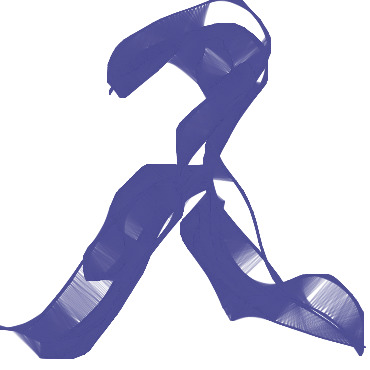
\includegraphics[height=12pt,clip]{lambda.jpg}
       \end{minipage}
       \begin{minipage}{0.8\textwidth}
         Based on a work at \href{https://gitlab.com/ualib/ualib.gitlab.io}{https://gitlab.com/ualib/ualib.gitlab.io}.
       \end{minipage}}
   \renewcommand{\headrulewidth}{0pt}
}}

%% \fancyfoot{\ccbysa{William J.~DeMeo}}
\pagestyle{fancy}
\renewcommand{\sectionmark}[1]{\markboth{#1}{}}
\fancyhf{}
\fancyhead[ER]{\sffamily\bfseries \leftmark}
\fancyhead[OL]{\sffamily\bfseries The Agda Universal Algebra Library}
\fancyhead[EL,OR]{\sffamily\bfseries \thepage}


\Copyright{William J. DeMeo}

\ccsdesc[500]{Theory of computation~Constructive mathematics}
\ccsdesc[500]{Theory of computation~Type theory}
\ccsdesc[500]{Theory of computation~Logic and verification}
\ccsdesc[300]{Computing methodologies~Representation of mathematical objects}
\ccsdesc[300]{Theory of computation~Type structures}


\keywords{Universal algebra, Equational logic, Martin-Löf Type Theory, Birkhoff’s HSP Theorem, Formalization of mathematics, Agda, Proof assistant}

\category{} %optional, e.g. invited paper

\relatedversion{hosted on arXiv}
\relatedversiondetails[linktext={arxiv.org/pdf/2101.10166}]{Extended Version}{https://arxiv.org/pdf/2101.10166}

\supplement{~\\ \textit{Documentation}: \ualibdotorg}%
\supplementdetails{Software}{https://gitlab.com/ualib/ualib.gitlab.io.git}

\acknowledgements{The author wishes to thank Cliff Bergman, Hyeyoung Shin, and Siva Somayyajula for supporting and contributing to this project, and \MartinEscardo for creating the \TypeTopology library and teaching a course on \href{https://www.cs.bham.ac.uk/~mhe/HoTT-UF-in-Agda-Lecture-Notes/index.html}{Univalent Foundations of Mathematics with Agda} at the \href{http://events.cs.bham.ac.uk/mgs2019/}{2019 Midlands Graduate School in Computing Science}. Of course, this work would not exist in its current form without the Agda 2 language by Ulf Norell.\footnote{Agda 2 is partially based on code from Agda 1 by Catarina Coquand and Makoto Takeyama, and from Agdalight by Ulf Norell and Andreas Abel.}}

\nolinenumbers %uncomment to disable line numbering

\hideLIPIcs  %uncomment to remove references to LIPIcs series (logo, DOI, ...), e.g. when preparing a pre-final version to be uploaded to arXiv or another public repository

%Editor-only macros:: begin (do not touch as author)%%%%%%%%%%%%%%%%%%%%%%%%%%%%%%%%%%
\EventEditors{}
\EventNoEds{2}
\EventLongTitle{}
\EventShortTitle{}
\EventAcronym{}
\EventYear{2021}
\EventDate{January 19, 2021}
\EventLocation{}
\EventLogo{}
\SeriesVolume{0}
\ArticleNo{0}
%%%%%%%%%%%%%%%%%%%%%%%%%%%%%%%%%%%%%%%%%%%%%%%%%%%%%%

\begin{document}

\maketitle


\begin{abstract}
The Agda Universal Algebra Library (\ualib) is a library of types and programs (theorems and proofs) we developed to formalize the foundations of universal algebra in Martin-Löf-style dependent type theory using the \agda programming language and proof assistant. This paper describes the \ualib and demonstrates that Agda is accessible to working mathematicians (such as ourselves) as a tool for formally verifying nontrivial results in general algebra and related fields. The library includes a substantial collection of definitions, theorems, and proofs from universal algebra and equational logic and as such provides many examples that exhibit the power of inductive and dependent types for representing and reasoning about general algebraic and relational structures.

The first major milestone of the \ualib project is a complete proof of Birkhoff's HSP theorem. To the best of our knowledge, this is the first time Birkhoff's theorem has been formulated and proved in dependent type theory and verified with a proof assistant.
%
%% In this paper we describe the \agdaualib and the formal proof of Birkhoff's theorem, discussing some of the technically challenging parts of the proof. In so doing, we illustrate the effectiveness of dependent type theory, Agda, and the \ualib for formally verifying nontrivial theorems in universal algebra and equational logic.
\end{abstract}



\section{Introduction}\label{sec:introduction}
To support formalization in type theory of research level mathematics in universal algebra and related fields, we present the Agda Universal Algebra Library (\agdaualib), a software library containing formal statements and proofs of the core definitions and results of universal algebra. 
The \ualib is written in \agda~\cite{Norell:2009}, a programming language and proof assistant based on Martin-L\"of Type Theory that not only supports dependent and inductive types, as well as proof tactics for proving things about the objects that inhabit these types.

There have been a number of efforts to formalize parts of universal algebra in type theory prior to ours, most notably
\begin{itemize}
  \item Capretta~\cite{Capretta:1999} (1999) formalized the basics of universal algebra in the Calculus of Inductive Constructions using the Coq proof assistant;
    \item Spitters and van der Weegen~\cite{Spitters:2011} (2011) formalized the basics of universal algebra and some classical algebraic structures, also in the Calculus of Inductive Constructions using the Coq proof assistant, promoting the use of type classes as a preferable alternative to setoids;
 \item Gunther, et al~\cite{Gunther:2018} (2018) developed what seems to be (prior to the \ualib) the most extensive library of formal universal algebra to date; in particular, this work includes a formalization of some basic equational logic; the project (like the \ualib) uses Martin-L\"of Type Theory and the Agda proof assistant.
\end{itemize}
Some other projects aimed at formalizing mathematics generally, and algebra in particular, have developed into very extensive libraries that include definitions, theorems, and proofs about algebraic structures, such as groups, rings, modules, etc.  However, the goals of these efforts seem to be the formalization of special classical algebraic structures, as opposed to the general theory of (universal) algebras. Moreover, the part of universal algebra and equational logic formalized in the \ualib extends beyond the scope of prior efforts and. In particular, the library now includes a proof of Birkhoff's variety theorem.  Most other proofs of this theorem that we know of are informal and nonconstructive.\footnote{After the completion of this work, the author learned about a constructive version of Birkhoff's theorem that was proved by Carlstr\"om in~\cite{Carlstrom:2008}.  The latter is presented in the standard, informal style of mathematical writing in the current literature, and as far as we know it was never implemented formally and type-checked with a proof assistant. Nonetheless, a comparison of the version of the theorem presented in~\cite{Carlstrom:2008} to the Agda proof we give here would be interesting. We remark briefly on this in~\S\ref{sec:conclusions-and-future-work}.}

%% \subsection{Vision and Goals}\label{vision-and-goals}
The seminal idea for the \agdaualib project was the observation that, on the one hand, a number of fundamental constructions in universal algebra can be defined recursively, and theorems about them proved by structural induction, while, on the other hand, inductive and dependent types make possible very precise formal representations of recursively defined objects, which often admit elegant constructive proofs of properties of such objects.  An important feature of such proofs in type theory is that they are total functional programs and, as such, they are computable and composable.
%% These observations suggested that there would be much to gain from implementing universal algebra in a language, such as Martin-L\"of type theory, that features dependent and inductive types.

Finally, our own research experience has taught us that a proof assistant and programming language (like Agda), when equipped with specialized libraries and domain-specific tactics to automate proof idioms of a particular field, can be an extremely powerful and effective asset. We believe that such libraries, and the proof assistants they support, will eventually become indispensable tools in the working mathematician's toolkit.



\subsection{Contributions and organization}
\label{sec:contributions}

Apart from the library itself, we describe the formal implementation and proof of a deep result, Garrett Birkhoff's celebrated HSP theorem~\cite{Birkhoff:1935}, which was among the first major results of universal algebra.  The theorem states that a \defn{variety} (a class of algebras closed under quotients, subalgebras, and products) is an equational class (defined by the set of identities satisfied by all its members).  %% More precisely, a class 𝒦 of algebras is closed under the taking of quotients, subalgebras, and arbitrary products if and only if 𝒦 is the class of algebras satisfying a certain set of equations.
The fact that we now have a formal proof of this is noteworthy, not only because this is the first time the theorem has been proved in dependent type theory and verified with a proof assistant, but also because the proof is constructive. As the paper~\cite{Carlstrom:2008} of Carlstr\"om makes clear, it is a highly nontrivial exercise to take a well-known informal proof of a theorem like Birkhoff's and show that it can be formalized using only constructive logic and natural deduction, without appealing to, say, the Law of the Excluded Middle or the Axiom of Choice.

Each of the sections that follow describes only what seem to us the most important or noteworthy components of the \ualib. Of course, space does not permit us to cover all aspects of the complete formal proof of a theorem like Birkhoff's.  We remedy this in two ways. First, throughout the paper we include pointers to places in the documentation where the omitted material can be found.  Second, we include an appendix describing special notation conventions and some of the more important types defined in the \ualib.  Finally, we highly recommend the book by Bergman~\cite{Bergman:2012} for background in universal algebra, and the notes by \escardo~\cite{MHE} for background in type theory and Agda.

The paper is structured as follows. Section~\ref{sec:agda-preliminaries} introduces Sigma types in Agda (for us, the most important dependent type in the language) as well as Agda's universe hierarchy. Section~\ref{sec:types-for-algebras} introduces the \agdaualib by explaining how algebraic structures are represented in the library. Section~\ref{sec:quotient-types-and-quotient-algebras} describes the approach we take to quotient types and quotient algebra types. Section~\ref{sec:homom-terms-subalg} defines new types that represent \emph{homomorphisms}, \emph{terms}, and \emph{subalgebras}, and Section~\ref{sec:equations-and-varieties} does the same for \emph{equational theories} and \emph{models}. This is also where we present free algebras, both in the informal theory (\S\ref{ssec:the-free-algebra-in-theory}) and represented as types in Agda (\S\ref{ssec:the-free-algebra-in-agda}). Finally, Section~\ref{sec:birkhoff} presents Birkhoff's theorem, describing the structure of the proof, with pointers to places in the documentation and source code where one can find the complete formal proof. The final section of the paper includes a few remarks about current work and future directions.

To conclude this introduction, we provide the following links to official sources of information about the \agdaualib.
\begin{itemize}
  \item \href{https://ualib.gitlab.io}{\texttt{ualib.org}} (the web site) includes every line of code in the library, rendered as html and accompanied by documentation, and
  \item \href{https://gitlab.com/ualib/ualib.gitlab.io}{\texttt{gitlab.com/ualib/ualib.gitlab.io}} (the source code) freely available and licensed under the \href{https://creativecommons.org/licenses/by-sa/4.0/}{Creative Commons Attribution-ShareAlike 4.0 International License}.
\end{itemize}
These sources include complete proofs of every theorem we mention here.







\section{Agda Preliminaries}\label{sec:agda-preliminaries}
For the benefit of readers who are not proficient in Agda and/or type theory, we briefly describe some of the most important types and features of Agda used in the \ualib.  Of necessity, some descriptions will be terse, but are usually accompanied by pointers to relevant sections of Appendix~\S\ref{sec:agda-prerequisites} or the \href{https://ualib.gitlab.io}{html documentation}.

We begin by highlighting some of the key parts of the \ualibPreliminaries module of the \ualib. This module imports everything we need from Martin Escardo's \typetopology library~\cite{MHE}, defines some other basic types and proves some of their properties.  We do not cover the entire Preliminaries module here, but call attention to aspects that differ from standard Agda syntax. For more details, see~\cite[\S2]{DeMeo:2021}.

Agda programs typically begin by setting some options and by importing from existing libraries.
Options are specified with the \AgdaKeyword{OPTIONS} \emph{pragma} and control the way Agda behaves by, for example, specifying which logical foundations should be assumed when the program is type-checked to verify its correctness. 
Every Agda program in the \ualib begins with the following pragma, which has the effects described below.
\ccpad
\begin{code}[number=code:options]
\>[0]\AgdaSymbol{\{-\#}\AgdaSpace{}%
\AgdaKeyword{OPTIONS}\AgdaSpace{}%
\AgdaPragma{--without-K}\AgdaSpace{}%
\AgdaPragma{--exact-split}\AgdaSpace{}%
\AgdaPragma{--safe}\AgdaSpace{}%
\AgdaSymbol{\#-\}}\<%
\end{code}
\\[-20pt]
%% \begin{enumerate}
\begin{itemize}
\item \AgdaPragma{without-K} disables \axiomk; see~\cite{agdaref-axiomk};
\item \AgdaPragma{exact-split} makes Agda accept only definitions that are \emph{judgmental} or \emph{definitional} equalities; see~\cite{agdatools-patternmatching};
  %% As \escardo explains, this ``makes sure that pattern matching corresponds to Martin-Löf eliminators;'' for more details
\item \AgdaPragma{safe} ensures that nothing is postulated outright---every non-MLTT axiom has to be an explicit assumption (e.g., an argument to a function or module); see~\cite{agdaref-safeagda} and~\cite{agdatools-patternmatching}.
\end{itemize}
%% \end{enumerate}
Throughout this paper we take assumptions 1--3 for granted without mentioning them explicitly.

\subsection{Agda's universe hierarchy}\label{ssec:agdas-universe-hierarchy}
The \agdaualib adopts the notation of Martin Escardo's \typetopology library~\cite{MHE}. In particular, \emph{universe levels}%
\footnote{See \href{https://agda.readthedocs.io/en/v2.6.1.2/language/universe-levels.html}{agda.readthedocs.io/en/v2.6.1.2/language/universe-levels.html}.}
are denoted by capitalized script letters from the second half of the alphabet, e.g., \ab 𝓤, \ab 𝓥, \ab 𝓦, etc.  Also defined in \typetopology are the operators~\af ̇~and~\af ⁺. These map a universe level \ab 𝓤 to the universe \ab 𝓤 \af ̇ := \Set \ab 𝓤 and the level \ab 𝓤 \af ⁺ \aod := \lsuc \ab 𝓤, respectively.  Thus, \ab 𝓤 \af ̇ is simply an alias for the universe \Set \ab 𝓤, and we have \ab 𝓤 \af ̇ \as : (\ab 𝓤 \af ⁺) \af ̇.
%% Table~\ref{tab:dictionary} translates between standard \agda syntax and \typetopology/\ualib notation.

The hierarchy of universes in Agda is structured as \ab{𝓤} \af ̇ \as : \ab 𝓤 \af ⁺\af ̇, \hskip3mm
\ab{𝓤} \af ⁺\af ̇ \as : \ab 𝓤 \af ⁺\af ⁺\af ̇, etc. This means that the universe \ab 𝓤 \af ̇ has type \ab 𝓤  \af ⁺\af ̇, and 𝓤 \af ⁺\af ̇ has type \ab 𝓤 \af ⁺\af ⁺\af ̇, and so on.  It is important to note, however, this does \emph{not} imply that \ab 𝓤 \af ̇ \as : \ab 𝓤 \af ⁺\af ⁺\af ̇. In other words, Agda's universe hierarchy is \emph{noncummulative}. This makes it possible to treat universe levels more generally and precisely, which is nice. On the other hand, a noncummulative hierarchy can sometimes make for a nonfun proof assistant. Luckily, there are ways to circumvent noncummulativity without introducing logical inconsistencies into the type theory. \S\ref{ssec:tools-for-noncummulative-universes} describes some domain specific tools that we developed for this purpose. (See also~\cite[\S3.3]{DeMeo:2021} for more details).




\subsection{Dependent pairs}\label{ssec:dependent-pairs}
Given universes \ab 𝓤 and \ab 𝓥, a type \ab X \as : \ab 𝓤 \aof ̇, and a type family \ab Y \as : X \as → \ab 𝓥 \aof ̇, the \defn{Sigma type} (or \defn{dependent pair type}) is denoted by \AgdaRecord{Σ}(\ab x \as ꞉ \ab X)\as ,\ab Y(\ab x) and generalizes the Cartesian product \ab X \as × \ab Y by allowing the type \ab Y(\ab x) of the second argument of the ordered pair (\ab x\as , \ab y) to depend on the value \ab x of the first.  That is, \AgdaRecord{Σ}(\ab x \as ꞉ \ab X)\as ,\ab Y(\ab x) is inhabited by pairs (\ab x\as , \ab y) such that \ab x \as : \ab X and \ab y \as : \ab Y(\ab x).

Agda's default syntax for a Sigma type is \AgdaRecord{Σ}\sP{3}\AgdaSymbol{λ}(\ab x\sP{3}꞉\sP{3}\ab X)\sP{3}\as →\sP{3}\ab Y, but we prefer the notation \AgdaRecord{Σ}~\ab x~꞉~\ab X~,~\ab Y, which is closer to the standard syntax described in the preceding paragraph. Fortunately, this preferred notation is available in the \typetopology library (see~\cite[Σ types]{MHE}).\footnote{The symbol \as ꞉ in the expression \AgdaRecord{Σ}\sP{3}\ab x\sP{3}\as ꞉\sP{3}\ab X\sP{3}\AgdaComma\sP{3}\ab Y is not the ordinary colon (:); rather, it is the symbol obtained by typing \texttt{\textbackslash{}:4} in \agdatwomode.} 

\newcommand\FstUnder{\AgdaOperator{\AgdaFunction{∣\AgdaUnderscore{}∣}}\xspace}
\newcommand\SndUnder{\AgdaOperator{\AgdaFunction{∥\AgdaUnderscore{}∥}}\xspace}
Convenient notations for the first and second projections out of a product are \FstUnder and \SndUnder, respectively. However, to improve readability or to avoid notation clashes with other modules, we sometimes use more standard alternatives, such as \AgdaFunction{pr₁} and \AgdaFunction{pr₂}, or \AgdaFunction{fst} and \AgdaFunction{snd}, or some combination of these. The definitions are standard so we omit them (see~\cite{DeMeo:2021} for details).














%%%%%%%%%%%%%%%%%%%%%%%%%%%%%%%%%%%%%%%%%%%%%%%%%%%%%%%%%%%%%%%%%%%%%%%%%%%%%%%%%%%%%%%%
%% Algebras %%%%%%%%%%%%%%%%%%%%%%%%%%%%%%%%%%%%%%%%%%%%%%%%%%%%%%%%%%%%%%%%%%%%%%%%%%%%
\section{Algebras}\label{sec:types-for-algebras}
A standard way to define algebraic structures in type theory is using record types.  However, we feel the dependent pair (or Sigma) type (\S\ref{ssec:dependent-pairs}) is more natural, as it corresponds semantically to the existential quantifier of logic. Therefore, many of the important types of the \ualib are defined as Sigma types. In this section, we use function types and Sigma types to define the types of \emph{operations} (\S\ref{sec:operation-type}), \emph{signatures} (\S\ref{signature-type}), \emph{algebras} (\S\ref{ssec:algebra-type}), and \emph{product algebras} (\S\ref{ssec:product-algebra-type}).

\subsection{Operation type}\label{sec:operation-type}
Here is how the type of \defn{operations} is defined in the \ualib.
\ccpad
\begin{code}%
\>[0]\AgdaFunction{Op}\AgdaSpace{}%
\AgdaSymbol{:}\AgdaSpace{}%
\AgdaBound{𝓥}\AgdaSpace{}%
\AgdaOperator{\AgdaFunction{̇}}\AgdaSpace{}%
\AgdaSymbol{→}\AgdaSpace{}%
\AgdaBound{𝓤}\AgdaSpace{}%
\AgdaOperator{\AgdaFunction{̇}}\AgdaSpace{}%
\AgdaSymbol{→}\AgdaSpace{}%
\AgdaBound{𝓤}\AgdaSpace{}%
\AgdaOperator{\AgdaPrimitive{⊔}}\AgdaSpace{}%
\AgdaBound{𝓥}\AgdaSpace{}%
\AgdaOperator{\AgdaFunction{̇}}\<%
\\
%
\>[0]\AgdaFunction{Op}\AgdaSpace{}%
\AgdaBound{I}\AgdaSpace{}%
\AgdaBound{A}\AgdaSpace{}%
\AgdaSymbol{=}\AgdaSpace{}%
\AgdaSymbol{(}\AgdaBound{I}\AgdaSpace{}%
\AgdaSymbol{→}\AgdaSpace{}%
\AgdaBound{A}\AgdaSymbol{)}\AgdaSpace{}%
\AgdaSymbol{→}\AgdaSpace{}%
\AgdaBound{A}
\end{code}
\ccpad
The type \AgdaFunction{Op} encodes the arity of an operation as an arbitrary type \ab I : \ab 𝓥 ̇, which gives us a very general way to represent an operation as a function type with domain \ab I → \ab A (the type of ``tuples'') and codomain \ab A.  For example, the type of \defn{projections} is defined using the \af{Op} type, as follows.
\ccpad
\begin{code}
\>[1]\AgdaFunction{π}\AgdaSpace{}%
\AgdaSymbol{:}\AgdaSpace{}%
\AgdaSymbol{\{}\AgdaBound{I}\AgdaSpace{}%
\AgdaSymbol{:}\AgdaSpace{}%
\AgdaBound{𝓥}\AgdaSpace{}%
\AgdaOperator{\AgdaFunction{̇}}\AgdaSpace{}%
\AgdaSymbol{\}}\AgdaSpace{}%
\AgdaSymbol{\{}\AgdaBound{A}\AgdaSpace{}%
\AgdaSymbol{:}\AgdaSpace{}%
\AgdaBound{𝓤}\AgdaSpace{}%
\AgdaOperator{\AgdaFunction{̇}}\AgdaSpace{}%
\AgdaSymbol{\}}\AgdaSpace{}%
\AgdaSymbol{→}\AgdaSpace{}%
\AgdaBound{I}\AgdaSpace{}%
\AgdaSymbol{→}\AgdaSpace{}%
\AgdaFunction{Op}\AgdaSpace{}%
\AgdaBound{I}\AgdaSpace{}%
\AgdaBound{A}\<%
\\
%
\>[1]\AgdaFunction{π}\AgdaSpace{}%
\AgdaBound{i}\AgdaSpace{}%
\AgdaBound{x}\AgdaSpace{}%
\AgdaSymbol{=}\AgdaSpace{}%
\AgdaBound{x}\AgdaSpace{}%
\AgdaBound{i}\<%
\end{code}
\ccpad
The last two lines of the code block above codify the \ab i-th \ab I-ary projection operation on \ab A.

\subsection{Signature type}\label{signature-type}
We define the type of (algebraic) \emph{signatures} as follows.
\ccpad
\begin{code}%
\>[0]\AgdaFunction{Signature}\AgdaSpace{}%
\AgdaSymbol{:}\AgdaSpace{}%
\AgdaSymbol{(}\AgdaBound{𝓞}\AgdaSpace{}%
\AgdaBound{𝓥}\AgdaSpace{}%
\AgdaSymbol{:}\AgdaSpace{}%
\AgdaPostulate{Universe}\AgdaSymbol{)}\AgdaSpace{}%
\AgdaSymbol{→}\AgdaSpace{}%
\AgdaSymbol{(}\AgdaBound{𝓞}\AgdaSpace{}%
\AgdaOperator{\AgdaPrimitive{⊔}}\AgdaSpace{}%
\AgdaBound{𝓥}\AgdaSymbol{)}\AgdaSpace{}%
\AgdaOperator{\AgdaPrimitive{⁺}}\AgdaSpace{}%
\AgdaOperator{\AgdaFunction{̇}}\<%
\\
\>[0]\AgdaFunction{Signature}\AgdaSpace{}%
\AgdaBound{𝓞}\AgdaSpace{}%
\AgdaBound{𝓥}\AgdaSpace{}%
\AgdaSymbol{=}\AgdaSpace{}%
\AgdaFunction{Σ}\AgdaSpace{}%
\AgdaBound{F}\AgdaSpace{}%
\AgdaFunction{꞉}\AgdaSpace{}%
\AgdaBound{𝓞}\AgdaSpace{}%
\AgdaOperator{\AgdaFunction{̇}}\AgdaSpace{}%
\AgdaFunction{,}\AgdaSpace{}%
\AgdaSymbol{(}\AgdaBound{F}\AgdaSpace{}%
\AgdaSymbol{→}\AgdaSpace{}%
\AgdaBound{𝓥}\AgdaSpace{}%
\AgdaOperator{\AgdaFunction{̇}}\AgdaSymbol{)}\<%
\end{code}
\ccpad
Here \AgdaBound{𝓞} is the universe level of operation symbol types, while \AgdaBound{𝓥} is the universe level of arity types. We denote the first and second projections by \ai ∣ and \ai ∥ (\S\ref{ssec:dependent-pairs}) so if \ab 𝑆 is a signature, then \aiab{∣}{𝑆} denotes the type of \defn{operation symbols}, and \aiab{∥}{𝑆} denotes the \defn{arity} function. If \ab 𝑓~\as :~\af ∣~\ab 𝑆~\af ∣ is an operation symbol in the signature \ab 𝑆, then \aiab{∥}{𝑆} \ab 𝑓 is the arity of \ab 𝑓. For example, %% \subsubsection{Example}\label{Signatures.sssec:example}
here is the signature of \emph{monoids}, as a member of the type \AgdaFunction{Signature} \AgdaBound{𝓞} \AgdaBound{𝓤₀}.
\ccpad
\begin{code}%
\>[0][@{}l@{\AgdaIndent{0}}]%
\>[1]\AgdaKeyword{data}\AgdaSpace{}%
\AgdaDatatype{monoid-op}\AgdaSpace{}%
\AgdaSymbol{:}\AgdaSpace{}%
\AgdaBound{𝓞}\AgdaSpace{}%
\AgdaOperator{\AgdaFunction{̇}}\AgdaSpace{}%
\AgdaKeyword{where}\<%
\\
\>[1][@{}l@{\AgdaIndent{0}}]%
\>[2]\AgdaInductiveConstructor{e}\AgdaSpace{}%
\AgdaSymbol{:}\AgdaSpace{}%
\AgdaDatatype{monoid-op}\<%
\\
%
\>[2]\AgdaInductiveConstructor{·}\AgdaSpace{}%
\AgdaSymbol{:}\AgdaSpace{}%
\AgdaDatatype{monoid-op}\<%
\\
%
\\[\AgdaEmptyExtraSkip]%
%
\>[1]\AgdaFunction{monoid-sig}\AgdaSpace{}%
\AgdaSymbol{:}\AgdaSpace{}%
\AgdaFunction{Signature}\AgdaSpace{}%
\AgdaBound{𝓞}\AgdaSpace{}%
\AgdaBound{𝓤₀}\<%
\\
%
\>[1]\AgdaFunction{monoid-sig}\AgdaSpace{}%
\AgdaSymbol{=}\AgdaSpace{}%
\AgdaDatatype{monoid-op}\AgdaSpace{}%
\AgdaOperator{\AgdaInductiveConstructor{,}}\AgdaSpace{}%
\AgdaSymbol{λ}\AgdaSpace{}%
\AgdaSymbol{\{}\AgdaSpace{}%
\AgdaInductiveConstructor{e}\AgdaSpace{}%
\AgdaSymbol{→}\AgdaSpace{}%
\AgdaFunction{𝟘}\AgdaSymbol{;}\AgdaSpace{}%
\AgdaInductiveConstructor{·}\AgdaSpace{}%
\AgdaSymbol{→}\AgdaSpace{}%
\AgdaFunction{𝟚}\AgdaSpace{}%
\AgdaSymbol{\}}\<%
\end{code}
\ccpad
This signature has two operation symbols, \aic e and \aic ·, and a function \as λ \as{\{} \AgdaInductiveConstructor{e} \as → \af 𝟘 \as ; \AgdaInductiveConstructor{·} \as → \af 𝟚 \as{\}} which maps \aic e to the empty type \af 𝟘 (since \aic e is nullary), and \aic · to the 2-element type \af 𝟚 (since \aic · is binary).








\newcommand\sigOV{\AgdaFunction{Signature}\AgdaSpace{}\AgdaBound{𝓞}\AgdaSpace{}\AgdaBound{𝓥}\xspace}
\subsection{Algebra type}\label{ssec:algebra-type}
For a fixed signature \ab S \as : \sigOV and universe \ab 𝓤, we define the type of \defn{algebras in the signature} \ab 𝑆 (or \ab 𝑆-\defn{algebras}) and with \defn{domain} (or \defn{carrier}) \ab 𝐴 \as : \ab 𝓤 \as ̇ as follows.\footnote{The \agdaualib includes an alternative definition of the type of algebras using records, but we don't discuss these here since they are not needed in the sequel. We refer the interested reader to~\cite{DeMeo:2021} and the html documentation available at \url{https://ualib.gitlab.io/UALib.Algebras.Algebras.html}.}
\ccpad
\begin{code}%
\>[0]\AgdaFunction{Algebra}\AgdaSpace{}%
\AgdaSymbol{:}\AgdaSpace{}%
\AgdaSymbol{(}\AgdaBound{𝓤}\AgdaSpace{}%
\AgdaSymbol{:}\AgdaSpace{}%
\AgdaPostulate{Universe}\AgdaSymbol{)(}\AgdaBound{𝑆}\AgdaSpace{}%
\AgdaSymbol{:}\AgdaSpace{}%
\AgdaFunction{Signature}\AgdaSpace{}%
\AgdaGeneralizable{𝓞}\AgdaSpace{}%
\AgdaGeneralizable{𝓥}\AgdaSymbol{)}\AgdaSpace{}%
\AgdaSymbol{→}%
\>[50]\AgdaGeneralizable{𝓞}\AgdaSpace{}%
\AgdaOperator{\AgdaPrimitive{⊔}}\AgdaSpace{}%
\AgdaGeneralizable{𝓥}\AgdaSpace{}%
\AgdaOperator{\AgdaPrimitive{⊔}}\AgdaSpace{}%
\AgdaBound{𝓤}\AgdaSpace{}%
\AgdaOperator{\AgdaPrimitive{⁺}}\AgdaSpace{}%
\AgdaOperator{\AgdaFunction{̇}}\<%
\\
%
\\[\AgdaEmptyExtraSkip]%
\>[0]\AgdaFunction{Algebra}\AgdaSpace{}%
\AgdaBound{𝓤}%
\>[13]\AgdaBound{𝑆}\AgdaSpace{}%
\AgdaSymbol{=}\AgdaSpace{}%
\AgdaFunction{Σ}\AgdaSpace{}%
\AgdaBound{A}\AgdaSpace{}%
\AgdaFunction{꞉}\AgdaSpace{}%
\AgdaBound{𝓤}\AgdaSpace{}%
\AgdaOperator{\AgdaFunction{̇}}\AgdaSpace{}%
\AgdaFunction{,}\AgdaSpace{}%
\AgdaSymbol{((}\AgdaBound{f}\AgdaSpace{}%
\AgdaSymbol{:}\AgdaSpace{}%
\AgdaOperator{\AgdaFunction{∣}}\AgdaSpace{}%
\AgdaBound{𝑆}\AgdaSpace{}%
\AgdaOperator{\AgdaFunction{∣}}\AgdaSymbol{)}\AgdaSpace{}%
\AgdaSymbol{→}\AgdaSpace{}%
\AgdaFunction{Op}\AgdaSpace{}%
\AgdaSymbol{(}\AgdaOperator{\AgdaFunction{∥}}\AgdaSpace{}%
\AgdaBound{𝑆}\AgdaSpace{}%
\AgdaOperator{\AgdaFunction{∥}}\AgdaSpace{}%
\AgdaBound{f}\AgdaSymbol{)}\AgdaSpace{}%
\AgdaBound{A}\AgdaSymbol{)}\<%
\end{code}
\ccpad
One could call an inhabitant of \af{Algebra} \ab 𝑆 \AgdaBound{𝓤} as an ``∞-algebra'' because its domain can be an arbitrary type, say, \ab A \as : \ab 𝓤 \af ̇ and need not be \emph{truncated} at some level (\S\ref{ssec:truncation-and-sets}). In particular, \ab A need not be an \emph{h-set} (as defined in \S\ref{ssec:truncation-and-sets}).%
%
\footnote{We could pause here to define the type of ``0-algebras,'' which are algebras whose domains are sets. This type is probably closer to what most of us think of when doing informal universal algebra. However, in the \ualib we have so far only needed to know that the domain of an algebra is a set in a handful of specific instances, so it seems preferable to work with general (∞-)algebras throughout the library and then assume \emph{uniqueness of identity proofs} explicitly where, and only where, a proof relies on this assumption.}

Next we define a convenient shorthand for the interpretation of an operation symbol. We use this often in the sequel.
\ccpad
\begin{code}%
\>[0][@{}l@{\AgdaIndent{1}}]%
\>[1]\AgdaOperator{\AgdaFunction{\AgdaUnderscore{}̂\AgdaUnderscore{}}}\AgdaSpace{}%
\AgdaSymbol{:}\AgdaSpace{}%
\AgdaSymbol{(}\AgdaBound{f}\AgdaSpace{}%
\AgdaSymbol{:}\AgdaSpace{}%
\AgdaOperator{\AgdaFunction{∣}}\AgdaSpace{}%
\AgdaBound{𝑆}\AgdaSpace{}%
\AgdaOperator{\AgdaFunction{∣}}\AgdaSymbol{)(}\AgdaBound{𝑨}\AgdaSpace{}%
\AgdaSymbol{:}\AgdaSpace{}%
\AgdaFunction{Algebra}\AgdaSpace{}%
\AgdaBound{𝓤}\AgdaSpace{}%
\AgdaBound{𝑆}\AgdaSymbol{)}\AgdaSpace{}%
\AgdaSymbol{→}\AgdaSpace{}%
\AgdaSymbol{(}\AgdaOperator{\AgdaFunction{∥}}\AgdaSpace{}%
\AgdaBound{𝑆}\AgdaSpace{}%
\AgdaOperator{\AgdaFunction{∥}}\AgdaSpace{}%
\AgdaBound{f}%
\>[48]\AgdaSymbol{→}%
\>[51]\AgdaOperator{\AgdaFunction{∣}}\AgdaSpace{}%
\AgdaBound{𝑨}\AgdaSpace{}%
\AgdaOperator{\AgdaFunction{∣}}\AgdaSymbol{)}\AgdaSpace{}%
\AgdaSymbol{→}\AgdaSpace{}%
\AgdaOperator{\AgdaFunction{∣}}\AgdaSpace{}%
\AgdaBound{𝑨}\AgdaSpace{}%
\AgdaOperator{\AgdaFunction{∣}}\<%
\\
%
\\[\AgdaEmptyExtraSkip]%
%
\>[1]\AgdaBound{f}\AgdaSpace{}%
\AgdaOperator{\AgdaFunction{̂}}\AgdaSpace{}%
\AgdaBound{𝑨}\AgdaSpace{}%
\AgdaSymbol{=}\AgdaSpace{}%
\AgdaSymbol{λ}\AgdaSpace{}%
\AgdaBound{x}\AgdaSpace{}%
\AgdaSymbol{→}\AgdaSpace{}%
\AgdaSymbol{(}\AgdaOperator{\AgdaFunction{∥}}\AgdaSpace{}%
\AgdaBound{𝑨}\AgdaSpace{}%
\AgdaOperator{\AgdaFunction{∥}}\AgdaSpace{}%
\AgdaBound{f}\AgdaSymbol{)}\AgdaSpace{}%
\AgdaBound{x}\<%
\end{code}
\ccpad
This is similar to the standard notation that one finds in the literature and seems much more natural to us than the double bar notation that we started with.

%% \subsection{Arbitrarily many variable symbols}
We assume that we always have at our disposal an arbitrary collection \ab X of variable symbols such that, for every algebra \ab 𝑨%% , no matter the type of its domain, 
we have a surjective map \ab{h₀} \as : \ab X \as → \aiab{∣}{𝑨} from variables onto the domain of \ab 𝑨.
\ccpad
\begin{code}%
\>[0][@{}l@{\AgdaIndent{1}}]%
\>[1]\AgdaOperator{\AgdaFunction{\AgdaUnderscore{}↠\AgdaUnderscore{}}}\AgdaSpace{}%
\AgdaSymbol{:}\AgdaSpace{}%
\AgdaSymbol{\{}\AgdaBound{𝓤}\AgdaSpace{}%
\AgdaBound{𝓧}\AgdaSpace{}%
\AgdaSymbol{:}\AgdaSpace{}%
\AgdaPostulate{Universe}\AgdaSymbol{\}}\AgdaSpace{}%
\AgdaSymbol{→}\AgdaSpace{}%
\AgdaBound{𝓧}\AgdaSpace{}%
\AgdaOperator{\AgdaFunction{̇}}\AgdaSpace{}%
\AgdaSymbol{→}\AgdaSpace{}%
\AgdaFunction{Algebra}\AgdaSpace{}%
\AgdaBound{𝓤}\AgdaSpace{}%
\AgdaBound{𝑆}\AgdaSpace{}%
\AgdaSymbol{→}\AgdaSpace{}%
\AgdaBound{𝓧}\AgdaSpace{}%
\AgdaOperator{\AgdaPrimitive{⊔}}\AgdaSpace{}%
\AgdaBound{𝓤}\AgdaSpace{}%
\AgdaOperator{\AgdaFunction{̇}}\<%
\\
%
\>[1]\AgdaBound{X}\AgdaSpace{}%
\AgdaOperator{\AgdaFunction{↠}}\AgdaSpace{}%
\AgdaBound{𝑨}\AgdaSpace{}%
\AgdaSymbol{=}\AgdaSpace{}%
\AgdaFunction{Σ}\AgdaSpace{}%
\AgdaBound{h}\AgdaSpace{}%
\AgdaFunction{꞉}\AgdaSpace{}%
\AgdaSymbol{(}\AgdaBound{X}\AgdaSpace{}%
\AgdaSymbol{→}\AgdaSpace{}%
\AgdaOperator{\AgdaFunction{∣}}\AgdaSpace{}%
\AgdaBound{𝑨}\AgdaSpace{}%
\AgdaOperator{\AgdaFunction{∣}}\AgdaSymbol{)}\AgdaSpace{}%
\AgdaFunction{,}\AgdaSpace{}%
\AgdaFunction{Epic}\AgdaSpace{}%
\AgdaBound{h}\<%
\end{code}

%%%%%%%%%%%%%%%%%%%%%%%%%%%%%%%%%%%%%%%%%%%%%%%%%%%%%%%%%%%%%%%%%%%%%%%%%%%%%%%%%%%%%
\subsection{Product algebra type}\label{ssec:product-algebra-type}
%% This section describes some parts of the \ualibAlgProducts module of the \agdaualib.
Suppose we are given a type \ab I \as : \ab 𝓘 (of ``indices'') and an indexed family \ab 𝒜 \as : \ab I \as → \af{Algebra} \ab 𝓤 \ab 𝑆 of \ab 𝑆-algebras. Then we define the \emph{product algebra}
\AgdaFunction{⨅} \AgdaBound{𝒜}
in the following natural way.%
%
\footnote{To distinguish the product algebra from the standard product type available in the \agdastdlib, instead of \af ∏ (\texttt{\textbackslash prod}) or \af Π (\texttt{\textbackslash Pi}), we use the symbol \AgdaFunction{⨅}, which is typed in \agdamode as \texttt{\textbackslash Glb}.}%
%
\ccpad
\begin{code}%
\>[1]\AgdaFunction{⨅}\AgdaSpace{}%
\AgdaSymbol{:}\AgdaSpace{}%
\AgdaSymbol{\{}\AgdaBound{𝓘}\AgdaSpace{}%
\AgdaSymbol{:}\AgdaSpace{}%
\AgdaPostulate{Universe}\AgdaSymbol{\}\{}\AgdaBound{I}\AgdaSpace{}%
\AgdaSymbol{:}\AgdaSpace{}%
\AgdaBound{𝓘}\AgdaSpace{}%
\AgdaOperator{\AgdaFunction{̇}}\AgdaSpace{}%
\AgdaSymbol{\}(}\AgdaBound{𝒜}\AgdaSpace{}%
\AgdaSymbol{:}\AgdaSpace{}%
\AgdaBound{I}\AgdaSpace{}%
\AgdaSymbol{→}\AgdaSpace{}%
\AgdaFunction{Algebra}\AgdaSpace{}%
\AgdaBound{𝓤}\AgdaSpace{}%
\AgdaBound{𝑆}\AgdaSpace{}%
\AgdaSymbol{)}\AgdaSpace{}%
\AgdaSymbol{→}\AgdaSpace{}%
\AgdaFunction{Algebra}\AgdaSpace{}%
\AgdaSymbol{(}\AgdaBound{𝓘}\AgdaSpace{}%
\AgdaOperator{\AgdaPrimitive{⊔}}\AgdaSpace{}%
\AgdaBound{𝓤}\AgdaSymbol{)}\AgdaSpace{}%
\AgdaBound{𝑆}\<%
\\
%
\>[1]\AgdaFunction{⨅}\AgdaSpace{}%
\AgdaSymbol{\{}\AgdaBound{𝓘}\AgdaSymbol{\}\{}\AgdaBound{I}\AgdaSymbol{\}}\AgdaSpace{}%
\AgdaBound{𝒜}\AgdaSpace{}%
\AgdaSymbol{=}\<%
\\
\>[1][@{}l@{\AgdaIndent{0}}]%
\>[2]\AgdaSymbol{((}\AgdaBound{i}\AgdaSpace{}%
\AgdaSymbol{:}\AgdaSpace{}%
\AgdaBound{I}\AgdaSymbol{)}\AgdaSpace{}%
\AgdaSymbol{→}\AgdaSpace{}%
\AgdaOperator{\AgdaFunction{∣}}\AgdaSpace{}%
\AgdaBound{𝒜}\AgdaSpace{}%
\AgdaBound{i}\AgdaSpace{}%
\AgdaOperator{\AgdaFunction{∣}}\AgdaSymbol{)}\AgdaSpace{}%
\AgdaOperator{\AgdaInductiveConstructor{,}}\AgdaSpace{}%
\AgdaSymbol{λ(}\AgdaBound{f}\AgdaSpace{}%
\AgdaSymbol{:}\AgdaSpace{}%
\AgdaOperator{\AgdaFunction{∣}}\AgdaSpace{}%
\AgdaBound{𝑆}\AgdaSpace{}%
\AgdaOperator{\AgdaFunction{∣}}\AgdaSymbol{)(}\AgdaBound{𝒂}\AgdaSpace{}%
\AgdaSymbol{:}\AgdaSpace{}%
\AgdaOperator{\AgdaFunction{∥}}\AgdaSpace{}%
\AgdaBound{𝑆}\AgdaSpace{}%
\AgdaOperator{\AgdaFunction{∥}}\AgdaSpace{}%
\AgdaBound{f}\AgdaSpace{}%
\AgdaSymbol{→}\AgdaSpace{}%
\AgdaSymbol{(}\AgdaBound{j}\AgdaSpace{}%
\AgdaSymbol{:}\AgdaSpace{}%
\AgdaBound{I}\AgdaSymbol{)}\AgdaSpace{}%
\AgdaSymbol{→}\AgdaSpace{}%
\AgdaOperator{\AgdaFunction{∣}}\AgdaSpace{}%
\AgdaBound{𝒜}\AgdaSpace{}%
\AgdaBound{j}\AgdaSpace{}%
\AgdaOperator{\AgdaFunction{∣}}\AgdaSymbol{)(}\AgdaBound{i}\AgdaSpace{}%
\AgdaSymbol{:}\AgdaSpace{}%
\AgdaBound{I}\AgdaSymbol{)}\AgdaSpace{}%
\AgdaSymbol{→}\AgdaSpace{}%
\AgdaSymbol{(}\AgdaBound{f}\AgdaSpace{}%
\AgdaOperator{\AgdaFunction{̂}}\AgdaSpace{}%
\AgdaBound{𝒜}\AgdaSpace{}%
\AgdaBound{i}\AgdaSymbol{)}\AgdaSpace{}%
\AgdaSymbol{λ\{}\AgdaBound{x}\AgdaSpace{}%
\AgdaSymbol{→}\AgdaSpace{}%
\AgdaBound{𝒂}\AgdaSpace{}%
\AgdaBound{x}\AgdaSpace{}%
\AgdaBound{i}\AgdaSymbol{\}}\<%
\end{code}
\ccpad
Here, the domain is the dependent function type
\af ∏ \af ∣ \ab 𝒜 \af ∣ := \AgdaSymbol{(}\AgdaBound{i}\AgdaSpace{}\AgdaSymbol{:}\AgdaSpace{}\AgdaBound{I}\AgdaSymbol{)}\AgdaSpace{}\AgdaSymbol{→}\AgdaSpace{}\AgdaOperator{\AgdaFunction{∣}}\AgdaSpace{}\AgdaBound{𝒜}\AgdaSpace{}\AgdaBound{i}\AgdaSpace{}\AgdaOperator{\AgdaFunction{∣}}
of ``tuples'', the \ab i-th components of which live in \af ∣ \ab 𝒜 \ab i \af ∣, and the operations are simply the operations of the \ab 𝒜~\ab i, interpreted component-wise.

The Birkhoff theorem involves products of entire arbitrary (nonindexed) classes of algebras, and it is not obvious how to handle this constructively, or whether it is even possible to do so without making extra assumptions about the class. (See~\cite{Carlstrom:2008} for a discussion of this issue.)  We describe our solution to this problem in \S~\ref{ssec:class-products-and-inclusions}.


\section{Quotient Types and Quotient Algebras}\label{sec:quotient-types-and-quotient-algebras}
For a binary relation \ab R on \ab A, we denote a single \ab R-class by \af [ \ab a \af ] \ab R (this denotes the class containing \ab a). We denote the type of all classes of a relation \ab R on \ab A by \af 𝒞 \as{\{} \ab A \as{\}} \as{\{} \ab R \as{\}}.  These are defined as in the \ualib as follows.
\ccpad
\begin{code}%
\>[1]\AgdaOperator{\AgdaFunction{[\AgdaUnderscore{}]}}\AgdaSpace{}%
\AgdaSymbol{:}\AgdaSpace{}%
\AgdaSymbol{\{}\AgdaBound{A}\AgdaSpace{}%
\AgdaSymbol{:}\AgdaSpace{}%
\AgdaBound{𝓤}\AgdaSpace{}%
\AgdaOperator{\AgdaFunction{̇}}\AgdaSpace{}%
\AgdaSymbol{\}}\AgdaSpace{}%
\AgdaSymbol{→}\AgdaSpace{}%
\AgdaBound{A}\AgdaSpace{}%
\AgdaSymbol{→}\AgdaSpace{}%
\AgdaFunction{Rel}\AgdaSpace{}%
\AgdaBound{A}\AgdaSpace{}%
\AgdaBound{𝓡}\AgdaSpace{}%
\AgdaSymbol{→}\AgdaSpace{}%
\AgdaFunction{Pred}\AgdaSpace{}%
\AgdaBound{A}\AgdaSpace{}%
\AgdaBound{𝓡}\<%
\\
%
\>[1]\AgdaOperator{\AgdaFunction{[}}\AgdaSpace{}%
\AgdaBound{a}\AgdaSpace{}%
\AgdaOperator{\AgdaFunction{]}}\AgdaSpace{}%
\AgdaBound{R}\AgdaSpace{}%
\AgdaSymbol{=}\AgdaSpace{}%
\AgdaSymbol{λ}\AgdaSpace{}%
\AgdaBound{x}\AgdaSpace{}%
\AgdaSymbol{→}\AgdaSpace{}%
\AgdaBound{R}\AgdaSpace{}%
\AgdaBound{a}\AgdaSpace{}%
\AgdaBound{x}\<%
\\
\\
\>[1]\AgdaFunction{𝒞}\AgdaSpace{}%
\AgdaSymbol{:}\AgdaSpace{}%
\AgdaSymbol{\{}\AgdaBound{A}\AgdaSpace{}%
\AgdaSymbol{:}\AgdaSpace{}%
\AgdaBound{𝓤}\AgdaSpace{}%
\AgdaOperator{\AgdaFunction{̇}}\AgdaSymbol{\}\{}\AgdaBound{R}\AgdaSpace{}%
\AgdaSymbol{:}\AgdaSpace{}%
\AgdaFunction{Rel}\AgdaSpace{}%
\AgdaBound{A}\AgdaSpace{}%
\AgdaBound{𝓡}\AgdaSymbol{\}}\AgdaSpace{}%
\AgdaSymbol{→}\AgdaSpace{}%
\AgdaFunction{Pred}\AgdaSpace{}%
\AgdaBound{A}\AgdaSpace{}%
\AgdaBound{𝓡}\AgdaSpace{}%
\AgdaSymbol{→}\AgdaSpace{}%
\AgdaSymbol{(}\AgdaBound{𝓤}\AgdaSpace{}%
\AgdaOperator{\AgdaPrimitive{⊔}}\AgdaSpace{}%
\AgdaBound{𝓡}\AgdaSpace{}%
\AgdaOperator{\AgdaPrimitive{⁺}}\AgdaSymbol{)}\AgdaSpace{}%
\AgdaOperator{\AgdaFunction{̇}}\<%
\\
%
\>[1]\AgdaFunction{𝒞}\AgdaSpace{}%
\AgdaSymbol{\{}\AgdaBound{A}\AgdaSymbol{\}\{}\AgdaBound{R}\AgdaSymbol{\}}\AgdaSpace{}%
\AgdaSymbol{=}\AgdaSpace{}%
\AgdaSymbol{λ}\AgdaSpace{}%
\AgdaSymbol{(}\AgdaBound{C}\AgdaSpace{}%
\AgdaSymbol{:}\AgdaSpace{}%
\AgdaFunction{Pred}\AgdaSpace{}%
\AgdaBound{A}\AgdaSpace{}%
\AgdaBound{𝓡}\AgdaSymbol{)}\AgdaSpace{}%
\AgdaSymbol{→}\AgdaSpace{}%
\AgdaFunction{Σ}\AgdaSpace{}%
\AgdaBound{a}\AgdaSpace{}%
\AgdaFunction{꞉}\AgdaSpace{}%
\AgdaBound{A}\AgdaSpace{}%
\AgdaFunction{,}\AgdaSpace{}%
\AgdaBound{C}\AgdaSpace{}%
\AgdaOperator{\AgdaDatatype{≡}}\AgdaSpace{}%
\AgdaSymbol{(}\AgdaSpace{}%
\AgdaOperator{\AgdaFunction{[}}\AgdaSpace{}%
\AgdaBound{a}\AgdaSpace{}%
\AgdaOperator{\AgdaFunction{]}}\AgdaSpace{}%
\AgdaBound{R}\AgdaSymbol{)}\<%
\end{code}
\ccpad
There are a few ways we could define the quotient with respect to a relation. We have found the following to be the most convenient.
\ccpad
\begin{code}%
\>[1]\AgdaOperator{\AgdaFunction{\AgdaUnderscore{}/\AgdaUnderscore{}}}\AgdaSpace{}%
\AgdaSymbol{:}\AgdaSpace{}%
\AgdaSymbol{(}\AgdaBound{A}\AgdaSpace{}%
\AgdaSymbol{:}\AgdaSpace{}%
\AgdaBound{𝓤}\AgdaSpace{}%
\AgdaOperator{\AgdaFunction{̇}}\AgdaSpace{}%
\AgdaSymbol{)}\AgdaSpace{}%
\AgdaSymbol{→}\AgdaSpace{}%
\AgdaFunction{Rel}\AgdaSpace{}%
\AgdaBound{A}\AgdaSpace{}%
\AgdaBound{𝓡}\AgdaSpace{}%
\AgdaSymbol{→}\AgdaSpace{}%
\AgdaBound{𝓤}\AgdaSpace{}%
\AgdaOperator{\AgdaPrimitive{⊔}}\AgdaSpace{}%
\AgdaSymbol{(}\AgdaBound{𝓡}\AgdaSpace{}%
\AgdaOperator{\AgdaPrimitive{⁺}}\AgdaSymbol{)}\AgdaSpace{}%
\AgdaOperator{\AgdaFunction{̇}}\<%
\\
%
\>[1]\AgdaBound{A}\AgdaSpace{}%
\AgdaOperator{\AgdaFunction{/}}\AgdaSpace{}%
\AgdaBound{R}\AgdaSpace{}%
\AgdaSymbol{=}\AgdaSpace{}%
\AgdaFunction{Σ}\AgdaSpace{}%
\AgdaBound{C}\AgdaSpace{}%
\AgdaFunction{꞉}\AgdaSpace{}%
\AgdaFunction{Pred}\AgdaSpace{}%
\AgdaBound{A}\AgdaSpace{}%
\AgdaBound{𝓡}\AgdaSpace{}%
\AgdaFunction{,}%
\>[27]\AgdaFunction{𝒞}\AgdaSymbol{\{}\AgdaBound{A}\AgdaSymbol{\}\{}\AgdaBound{R}\AgdaSymbol{\}}\AgdaSpace{}%
\AgdaBound{C}\<%
\end{code}
\ccpad
We then have the following introduction and elimination rules for a class with a designated representative.
\ccpad
\begin{code}%
\>[0][@{}l@{\AgdaIndent{1}}]%
\>[1]\AgdaOperator{\AgdaFunction{⟦\AgdaUnderscore{}⟧}}\AgdaSpace{}%
\AgdaSymbol{:}\AgdaSpace{}%
\AgdaSymbol{\{}\AgdaBound{A}\AgdaSpace{}%
\AgdaSymbol{:}\AgdaSpace{}%
\AgdaBound{𝓤}\AgdaSpace{}%
\AgdaOperator{\AgdaFunction{̇}}\AgdaSymbol{\}}\AgdaSpace{}%
\AgdaSymbol{→}\AgdaSpace{}%
\AgdaBound{A}\AgdaSpace{}%
\AgdaSymbol{→}\AgdaSpace{}%
\AgdaSymbol{\{}\AgdaBound{R}\AgdaSpace{}%
\AgdaSymbol{:}\AgdaSpace{}%
\AgdaFunction{Rel}\AgdaSpace{}%
\AgdaBound{A}\AgdaSpace{}%
\AgdaBound{𝓡}\AgdaSymbol{\}}\AgdaSpace{}%
\AgdaSymbol{→}\AgdaSpace{}%
\AgdaBound{A}\AgdaSpace{}%
\AgdaOperator{\AgdaFunction{/}}\AgdaSpace{}%
\AgdaBound{R}\<%
\\
%
\>[1]\AgdaOperator{\AgdaFunction{⟦}}\AgdaSpace{}%
\AgdaBound{a}\AgdaSpace{}%
\AgdaOperator{\AgdaFunction{⟧}}\AgdaSpace{}%
\AgdaSymbol{\{}\AgdaBound{R}\AgdaSymbol{\}}\AgdaSpace{}%
\AgdaSymbol{=}\AgdaSpace{}%
\AgdaSymbol{(}\AgdaOperator{\AgdaFunction{[}}\AgdaSpace{}%
\AgdaBound{a}\AgdaSpace{}%
\AgdaOperator{\AgdaFunction{]}}\AgdaSpace{}%
\AgdaBound{R}\AgdaSymbol{)}\AgdaSpace{}%
\AgdaOperator{\AgdaInductiveConstructor{,}}\AgdaSpace{}%
\AgdaBound{a}\AgdaSpace{}%
\AgdaOperator{\AgdaInductiveConstructor{,}}\AgdaSpace{}%
\AgdaInductiveConstructor{𝓇ℯ𝒻𝓁}\<%
\end{code}
\ccpad
\begin{code}
\>[1]\AgdaOperator{\AgdaFunction{⌜\AgdaUnderscore{}⌝}}\AgdaSpace{}%
\AgdaSymbol{:}\AgdaSpace{}%
\AgdaSymbol{\{}\AgdaBound{A}\AgdaSpace{}%
\AgdaSymbol{:}\AgdaSpace{}%
\AgdaBound{𝓤}\AgdaSpace{}%
\AgdaOperator{\AgdaFunction{̇}}\AgdaSymbol{\}\{}\AgdaBound{R}\AgdaSpace{}%
\AgdaSymbol{:}\AgdaSpace{}%
\AgdaFunction{Rel}\AgdaSpace{}%
\AgdaBound{A}\AgdaSpace{}%
\AgdaBound{𝓡}\AgdaSymbol{\}}\AgdaSpace{}%
\AgdaSymbol{→}\AgdaSpace{}%
\AgdaBound{A}\AgdaSpace{}%
\AgdaOperator{\AgdaFunction{/}}\AgdaSpace{}%
\AgdaBound{R}%
\>[39]\AgdaSymbol{→}\AgdaSpace{}%
\AgdaBound{A}\<%
\\
%
\>[1]\AgdaOperator{\AgdaFunction{⌜}}\AgdaSpace{}%
\AgdaBound{𝒂}\AgdaSpace{}%
\AgdaOperator{\AgdaFunction{⌝}}\AgdaSpace{}%
\AgdaSymbol{=}\AgdaSpace{}%
\AgdaOperator{\AgdaFunction{∣}}\AgdaSpace{}%
\AgdaOperator{\AgdaFunction{∥}}\AgdaSpace{}%
\AgdaBound{𝒂}\AgdaSpace{}%
\AgdaOperator{\AgdaFunction{∥}}\AgdaSpace{}%
\AgdaOperator{\AgdaFunction{∣}}%
\end{code}














\subsection{Quotient extensionality}\label{ssec:quotient-extensionality}
We will need a subsingleton identity type for congruence classes over sets so that we can equate two classes, even when they are presented using different representatives. For this we assume that our relations are on sets, rather than arbitrary types. As mentioned earlier, this is equivalent to assuming that there is at most one proof that two elements of a set are the same.  The following \emph{class extensionality principle} accomplishes this for us.
\ccpad
\begin{code}%
\>[1]\AgdaFunction{class-extensionality'}\AgdaSpace{}%
\AgdaSymbol{:}%
\>[356I]\AgdaFunction{propext}\AgdaSpace{}%
\AgdaBound{𝓡}\AgdaSpace{}%
\AgdaSymbol{→}\AgdaSpace{}%
\AgdaFunction{global-dfunext}\AgdaSpace{}%
\AgdaSymbol{→}\AgdaSpace{}%
\AgdaSymbol{\{}\AgdaBound{A}\AgdaSpace{}%
\AgdaSymbol{:}\AgdaSpace{}%
\AgdaBound{𝓤}\AgdaSpace{}%
\AgdaOperator{\AgdaFunction{̇}}\AgdaSymbol{\}\{}\AgdaBound{a}\AgdaSpace{}%
\AgdaBound{a'}\AgdaSpace{}%
\AgdaSymbol{:}\AgdaSpace{}%
\AgdaBound{A}\AgdaSymbol{\}\{}\AgdaBound{R}\AgdaSpace{}%
\AgdaSymbol{:}\AgdaSpace{}%
\AgdaFunction{Rel}\AgdaSpace{}%
\AgdaBound{A}\AgdaSpace{}%
\AgdaBound{𝓡}\AgdaSymbol{\}}\<%
\\
\>[1][@{}l@{\AgdaIndent{0}}]%
\>[2]\AgdaSymbol{→}%
\>[.][@{}l@{}]\<[356I]%
\>[25]\AgdaSymbol{(∀}\AgdaSpace{}%
\AgdaBound{a}\AgdaSpace{}%
\AgdaBound{x}\AgdaSpace{}%
\AgdaSymbol{→}\AgdaSpace{}%
\AgdaFunction{is-subsingleton}\AgdaSpace{}%
\AgdaSymbol{(}\AgdaBound{R}\AgdaSpace{}%
\AgdaBound{a}\AgdaSpace{}%
\AgdaBound{x}\AgdaSymbol{))}\AgdaSpace{}%
\AgdaSymbol{→}\AgdaSpace{}%
\AgdaSymbol{(∀}\AgdaSpace{}%
\AgdaBound{C}\AgdaSpace{}%
\AgdaSymbol{→}\AgdaSpace{}%
\AgdaFunction{is-subsingleton}\AgdaSpace{}%
\AgdaSymbol{(}\AgdaFunction{𝒞}\AgdaSpace{}%
\AgdaBound{C}\AgdaSymbol{))}\<%
\\
%
\>[2]\AgdaSymbol{→}%
\>[25]\AgdaRecord{IsEquivalence}\AgdaSpace{}%
\AgdaBound{R}\<%
\\
%
\>[25]\AgdaComment{----------------------------}\<%
\\
%
\>[2]\AgdaSymbol{→}%
\>[25]\AgdaBound{R}\AgdaSpace{}%
\AgdaBound{a}\AgdaSpace{}%
\AgdaBound{a'}\AgdaSpace{}%
\AgdaSymbol{→}\AgdaSpace{}%
\AgdaSymbol{(}\AgdaOperator{\AgdaFunction{⟦}}\AgdaSpace{}%
\AgdaBound{a}\AgdaSpace{}%
\AgdaOperator{\AgdaFunction{⟧}}\AgdaSpace{}%
\AgdaSymbol{\{}\AgdaBound{R}\AgdaSymbol{\})}\AgdaSpace{}%
\AgdaOperator{\AgdaDatatype{≡}}\AgdaSpace{}%
\AgdaSymbol{(}\AgdaOperator{\AgdaFunction{⟦}}\AgdaSpace{}%
\AgdaBound{a'}\AgdaSpace{}%
\AgdaOperator{\AgdaFunction{⟧}}\AgdaSpace{}%
\AgdaSymbol{\{}\AgdaBound{R}\AgdaSymbol{\})}\<%

\end{code}
\ccpad
We omit the proof. \seedocfordetails



\subsection{Compatibility}\label{ssec:compatibility}
We say that a (unary) operation \ab f \as : \ab X \as → \ab X is \defn{compatible} with (or \defn{respects}, or \defn{preserves}) the binary relation \ab R on \ab X just in case \as ∀ \ab x, \ab y \as : X, we have \ab R \ab x \ab y \as →  \ab R (\ab f \ab x) (\ab f \ab y).  Now suppose \ab 𝓤, \ab 𝓥, and \ab 𝓦 are universes and assume the following typing judgments: \ab γ \as : \ab 𝓥 \af ̇, \ab X \as : \ab 𝓤 \af ̇. We lift the definition of compatibility from unary to \ab γ-ary operations in the following obvious way: for all \ab u \ab v \as : \ab γ \as → \ab X (\ab γ-tuples of \ab X), we say that the pair \ab u \ab v is \ab R-related, and we write \AgdaFunction{lift-rel}~\ab R~\ab u~\ab v provided \as ∀ \ab i \as : \ab γ, \ab R (\ab u \ab i) (\ab v \ab i). The function \af{lift-rel} is defined as follows.
\ccpad
\begin{code}%
\>[1]\AgdaFunction{lift-rel}\AgdaSpace{}%
\AgdaSymbol{:}\AgdaSpace{}%
\AgdaFunction{Rel}\AgdaSpace{}%
\AgdaBound{Z}\AgdaSpace{}%
\AgdaBound{𝓦}\AgdaSpace{}%
\AgdaSymbol{→}\AgdaSpace{}%
\AgdaSymbol{(}\AgdaBound{γ}\AgdaSpace{}%
\AgdaSymbol{→}\AgdaSpace{}%
\AgdaBound{Z}\AgdaSymbol{)}\AgdaSpace{}%
\AgdaSymbol{→}\AgdaSpace{}%
\AgdaSymbol{(}\AgdaBound{γ}\AgdaSpace{}%
\AgdaSymbol{→}\AgdaSpace{}%
\AgdaBound{Z}\AgdaSymbol{)}\AgdaSpace{}%
\AgdaSymbol{→}\AgdaSpace{}%
\AgdaBound{𝓥}\AgdaSpace{}%
\AgdaOperator{\AgdaPrimitive{⊔}}\AgdaSpace{}%
\AgdaBound{𝓦}\AgdaSpace{}%
\AgdaOperator{\AgdaFunction{̇}}\<%
\\
%
\>[1]\AgdaFunction{lift-rel}\AgdaSpace{}%
\AgdaBound{R}\AgdaSpace{}%
\AgdaBound{f}\AgdaSpace{}%
\AgdaBound{g}\AgdaSpace{}%
\AgdaSymbol{=}\AgdaSpace{}%
\AgdaSymbol{∀}\AgdaSpace{}%
\AgdaBound{x}\AgdaSpace{}%
\AgdaSymbol{→}\AgdaSpace{}%
\AgdaBound{R}\AgdaSpace{}%
\AgdaSymbol{(}\AgdaBound{f}\AgdaSpace{}%
\AgdaBound{x}\AgdaSymbol{)}\AgdaSpace{}%
\AgdaSymbol{(}\AgdaBound{g}\AgdaSpace{}%
\AgdaBound{x}\AgdaSymbol{)}\<%
\end{code}
\ccpad
If \ab f \as : (\ab γ \as → \ab X) \as → \ab X is a \ab γ-ary operation on \ab X, we say that \ab f is \defn{compatible} with \ab R provided for all \ab u \ab v : \ab γ \as → \ab X, \af{lift-rel} \ab R \ab u \ab v implies \ab R (\ab f \ab u) (\ab f \ab v).
\ccpad
\begin{code}
\>[1]\AgdaFunction{compatible-op}\AgdaSpace{}%
\AgdaSymbol{:}\AgdaSpace{}%
\AgdaSymbol{\{}\AgdaBound{𝑨}\AgdaSpace{}%
\AgdaSymbol{:}\AgdaSpace{}%
\AgdaFunction{Algebra}\AgdaSpace{}%
\AgdaBound{𝓤}\AgdaSpace{}%
\AgdaBound{𝑆}\AgdaSymbol{\}}\AgdaSpace{}%
\AgdaSymbol{→}\AgdaSpace{}%
\AgdaOperator{\AgdaFunction{∣}}\AgdaSpace{}%
\AgdaBound{𝑆}\AgdaSpace{}%
\AgdaOperator{\AgdaFunction{∣}}\AgdaSpace{}%
\AgdaSymbol{→}\AgdaSpace{}%
\AgdaFunction{Rel}\AgdaSpace{}%
\AgdaOperator{\AgdaFunction{∣}}\AgdaSpace{}%
\AgdaBound{𝑨}\AgdaSpace{}%
\AgdaOperator{\AgdaFunction{∣}}\AgdaSpace{}%
\AgdaBound{𝓦}\AgdaSpace{}%
\AgdaSymbol{→}\AgdaSpace{}%
\AgdaBound{𝓤}\AgdaSpace{}%
\AgdaOperator{\AgdaPrimitive{⊔}}\AgdaSpace{}%
\AgdaBound{𝓥}\AgdaSpace{}%
\AgdaOperator{\AgdaPrimitive{⊔}}\AgdaSpace{}%
\AgdaBound{𝓦}\AgdaSpace{}%
\AgdaOperator{\AgdaFunction{̇}}\<%
\\
%
\>[1]\AgdaFunction{compatible-op}\AgdaSpace{}%
\AgdaSymbol{\{}\AgdaBound{𝑨}\AgdaSymbol{\}}\AgdaSpace{}%
\AgdaBound{f}\AgdaSpace{}%
\AgdaBound{R}\AgdaSpace{}%
\AgdaSymbol{=}\AgdaSpace{}%
\AgdaSymbol{∀\{}\AgdaBound{𝒂}\AgdaSymbol{\}\{}\AgdaBound{𝒃}\AgdaSymbol{\}}\AgdaSpace{}%
\AgdaSymbol{→}\AgdaSpace{}%
\AgdaSymbol{(}\AgdaFunction{lift-rel}\AgdaSpace{}%
\AgdaBound{R}\AgdaSymbol{)}\AgdaSpace{}%
\AgdaBound{𝒂}\AgdaSpace{}%
\AgdaBound{𝒃}%
\>[53]\AgdaSymbol{→}\AgdaSpace{}%
\AgdaBound{R}\AgdaSpace{}%
\AgdaSymbol{((}\AgdaBound{f}\AgdaSpace{}%
\AgdaOperator{\AgdaFunction{̂}}\AgdaSpace{}%
\AgdaBound{𝑨}\AgdaSymbol{)}\AgdaSpace{}%
\AgdaBound{𝒂}\AgdaSymbol{)}\AgdaSpace{}%
\AgdaSymbol{((}\AgdaBound{f}\AgdaSpace{}%
\AgdaOperator{\AgdaFunction{̂}}\AgdaSpace{}%
\AgdaBound{𝑨}\AgdaSymbol{)}\AgdaSpace{}%
\AgdaBound{𝒃}\AgdaSymbol{)}\<%
\end{code}
\ccpad
Finally, to represent that all basic operations of an algebra are compatible with a given relation, we define
\ccpad
\begin{code}
\>[1]\AgdaFunction{compatible}\AgdaSpace{}%
\AgdaSymbol{:}{\AgdaSpace{}}%
\AgdaSymbol{(}\AgdaBound{𝑨}\AgdaSpace{}%
\AgdaSymbol{:}\AgdaSpace{}%
\AgdaFunction{Algebra}\AgdaSpace{}%
\AgdaBound{𝓤}\AgdaSpace{}%
\AgdaBound{𝑆}\AgdaSymbol{)}\AgdaSpace{}%
\AgdaSymbol{→}\AgdaSpace{}%
\AgdaFunction{Rel}\AgdaSpace{}%
\AgdaOperator{\AgdaFunction{∣}}\AgdaSpace{}%
\AgdaBound{𝑨}\AgdaSpace{}%
\AgdaOperator{\AgdaFunction{∣}}\AgdaSpace{}%
\AgdaBound{𝓦}\AgdaSpace{}%
\AgdaSymbol{→}\AgdaSpace{}%
\AgdaBound{𝓞}\AgdaSpace{}%
\AgdaOperator{\AgdaPrimitive{⊔}}\AgdaSpace{}%
\AgdaBound{𝓤}\AgdaSpace{}%
\AgdaOperator{\AgdaPrimitive{⊔}}\AgdaSpace{}%
\AgdaBound{𝓥}\AgdaSpace{}%
\AgdaOperator{\AgdaPrimitive{⊔}}\AgdaSpace{}%
\AgdaBound{𝓦}\AgdaSpace{}%
\AgdaOperator{\AgdaFunction{̇}}\<%
\\
%
\>[1]\AgdaFunction{compatible}%
\>[13]\AgdaBound{𝑨}\AgdaSpace{}%
\AgdaBound{R}\AgdaSpace{}%
\AgdaSymbol{=}\AgdaSpace{}%
\AgdaSymbol{∀}\AgdaSpace{}%
\AgdaBound{f}\AgdaSpace{}%
\AgdaSymbol{→}\AgdaSpace{}%
\AgdaFunction{compatible-op}\AgdaSymbol{\{}\AgdaBound{𝑨}\AgdaSymbol{\}}\AgdaSpace{}%
\AgdaBound{f}\AgdaSpace{}%
\AgdaBound{R}\<%
\end{code}
\ccpad
We'll see this definition of compatibility at work very soon when we define congruence relations in the next section.


\subsection{Congruence relations}\label{ssec:congr-relat}
This \ualibCongruences module of the \agdaualib defines a number of alternative representations of congruence relations of an algebra. We will only have occasion to use the Sigma and record type representations, which are defined as follows.
\ccpad
\begin{code}%
  This section describes parts of the \ualibCongruences module of the \agdaualib.
For more details, see \url{https://ualib.gitlab.io/UALib.Algebras.Congruences.html}.

A congruence relation of an algebra can be represented in a number of different ways. Here is a Sigma type and a record type, each of which can be used to represent congruence relations.
\ccpad
\begin{code}%
\>[0]\AgdaFunction{Con}\AgdaSpace{}%
\AgdaSymbol{:}\AgdaSpace{}%
\AgdaSymbol{\{}\AgdaBound{𝓤}\AgdaSpace{}%
\AgdaSymbol{:}\AgdaSpace{}%
\AgdaFunction{Universe}\AgdaSymbol{\}(}\AgdaBound{A}\AgdaSpace{}%
\AgdaSymbol{:}\AgdaSpace{}%
\AgdaFunction{Algebra}\AgdaSpace{}%
\AgdaBound{𝓤}\AgdaSpace{}%
\AgdaBound{𝑆}\AgdaSymbol{)}\AgdaSpace{}%
\AgdaSymbol{→}\AgdaSpace{}%
\AgdaFunction{ov}\AgdaSpace{}%
\AgdaBound{𝓤}\AgdaSpace{}%
\AgdaOperator{\AgdaFunction{̇}}\<%
\\
\>[0]\AgdaFunction{Con}\AgdaSpace{}%
\AgdaSymbol{\{}\AgdaBound{𝓤}\AgdaSymbol{\}}\AgdaSpace{}%
\AgdaBound{A}\AgdaSpace{}%
\AgdaSymbol{=}\AgdaSpace{}%
\AgdaFunction{Σ}\AgdaSpace{}%
\AgdaBound{θ}\AgdaSpace{}%
\AgdaFunction{꞉}\AgdaSpace{}%
\AgdaSymbol{(}\AgdaSpace{}%
\AgdaFunction{Rel}\AgdaSpace{}%
\AgdaOperator{\AgdaFunction{∣}}\AgdaSpace{}%
\AgdaBound{A}\AgdaSpace{}%
\AgdaOperator{\AgdaFunction{∣}}\AgdaSpace{}%
\AgdaBound{𝓤}\AgdaSpace{}%
\AgdaSymbol{)}\AgdaSpace{}%
\AgdaFunction{,}\AgdaSpace{}%
\AgdaRecord{IsEquivalence}\AgdaSpace{}%
\AgdaBound{θ}\AgdaSpace{}%
\AgdaOperator{\AgdaFunction{×}}\AgdaSpace{}%
\AgdaFunction{compatible}\AgdaSpace{}%
\AgdaBound{A}\AgdaSpace{}%
\AgdaBound{θ}\<%
\\
%
\\[\AgdaEmptyExtraSkip]%
\>[0]\AgdaKeyword{record}\AgdaSpace{}%
\AgdaRecord{Congruence}\AgdaSpace{}%
\AgdaSymbol{\{}\AgdaBound{𝓤}\AgdaSpace{}%
\AgdaBound{𝓦}\AgdaSpace{}%
\AgdaSymbol{:}\AgdaSpace{}%
\AgdaFunction{Universe}\AgdaSymbol{\}}\AgdaSpace{}%
\AgdaSymbol{(}\AgdaBound{A}\AgdaSpace{}%
\AgdaSymbol{:}\AgdaSpace{}%
\AgdaFunction{Algebra}\AgdaSpace{}%
\AgdaBound{𝓤}\AgdaSpace{}%
\AgdaBound{𝑆}\AgdaSymbol{)}\AgdaSpace{}%
\AgdaSymbol{:}\AgdaSpace{}%
\AgdaFunction{ov}\AgdaSpace{}%
\AgdaBound{𝓦}\AgdaSpace{}%
\AgdaOperator{\AgdaFunction{⊔}}\AgdaSpace{}%
\AgdaBound{𝓤}\AgdaSpace{}%
\AgdaOperator{\AgdaFunction{̇}}%
\>[67]\AgdaKeyword{where}\<%
\\
\>[0][@{}l@{\AgdaIndent{0}}]%
\>[1]\AgdaKeyword{constructor}\AgdaSpace{}%
\AgdaInductiveConstructor{mkcon}\<%
\\
%
\>[1]\AgdaKeyword{field}\<%
\\
\>[1][@{}l@{\AgdaIndent{0}}]%
\>[2]\AgdaOperator{\AgdaField{⟨\AgdaUnderscore{}⟩}}\AgdaSpace{}%
\AgdaSymbol{:}\AgdaSpace{}%
\AgdaFunction{Rel}\AgdaSpace{}%
\AgdaOperator{\AgdaFunction{∣}}\AgdaSpace{}%
\AgdaBound{A}\AgdaSpace{}%
\AgdaOperator{\AgdaFunction{∣}}\AgdaSpace{}%
\AgdaBound{𝓦}\<%
\\
%
\>[2]\AgdaField{Compatible}\AgdaSpace{}%
\AgdaSymbol{:}\AgdaSpace{}%
\AgdaFunction{compatible}\AgdaSpace{}%
\AgdaBound{A}\AgdaSpace{}%
\AgdaOperator{\AgdaField{⟨\AgdaUnderscore{}⟩}}\<%
\\
%
\>[2]\AgdaField{IsEquiv}\AgdaSpace{}%
\AgdaSymbol{:}\AgdaSpace{}%
\AgdaRecord{IsEquivalence}\AgdaSpace{}%
\AgdaOperator{\AgdaField{⟨\AgdaUnderscore{}⟩}}\<%
\end{code}


\subsubsection{Examples}\label{examples}

We defined the zero relation \af{𝟎-rel} above (\S\ref{kernels}). We now demonstrate how one constructs the \textit{trivial congruence} out of this relation. The relation \af{𝟎-rel} is equivalent to the identity relation \af ≡ and these are obviously both equivalences. In fact, we already proved this of ≡ in the \ualibEquality module, so we simply apply the corresponding proofs.
\ccpad
\begin{code}%
\>[1]\AgdaFunction{𝟎-IsEquivalence}\AgdaSpace{}%
\AgdaSymbol{:}\AgdaSpace{}%
\AgdaSymbol{\{}\AgdaBound{A}\AgdaSpace{}%
\AgdaSymbol{:}\AgdaSpace{}%
\AgdaBound{𝓤}\AgdaSpace{}%
\AgdaOperator{\AgdaFunction{̇}}\AgdaSpace{}%
\AgdaSymbol{\}}\AgdaSpace{}%
\AgdaSymbol{→}\AgdaSpace{}%
\AgdaRecord{IsEquivalence}\AgdaSymbol{\{}\AgdaBound{𝓤}\AgdaSymbol{\}\{}\AgdaArgument{A}\AgdaSpace{}%
\AgdaSymbol{=}\AgdaSpace{}%
\AgdaBound{A}\AgdaSymbol{\}}\AgdaSpace{}%
\AgdaFunction{𝟎-rel}\<%
\\
%
\>[1]\AgdaFunction{𝟎-IsEquivalence}\AgdaSpace{}%
\AgdaSymbol{=}\AgdaSpace{}%
\AgdaKeyword{record}\AgdaSpace{}%
\AgdaSymbol{\{}\AgdaSpace{}%
\AgdaField{rfl}\AgdaSpace{}%
\AgdaSymbol{=}\AgdaSpace{}%
\AgdaFunction{≡-rfl}\AgdaSymbol{;}\AgdaSpace{}%
\AgdaField{sym}\AgdaSpace{}%
\AgdaSymbol{=}\AgdaSpace{}%
\AgdaFunction{≡-sym}\AgdaSymbol{;}\AgdaSpace{}%
\AgdaField{trans}\AgdaSpace{}%
\AgdaSymbol{=}\AgdaSpace{}%
\AgdaFunction{≡-trans}\AgdaSpace{}%
\AgdaSymbol{\}}\<%
\\
%
\\[\AgdaEmptyExtraSkip]%
%
\>[1]\AgdaFunction{≡-IsEquivalence}\AgdaSpace{}%
\AgdaSymbol{:}\AgdaSpace{}%
\AgdaSymbol{\{}\AgdaBound{A}\AgdaSpace{}%
\AgdaSymbol{:}\AgdaSpace{}%
\AgdaBound{𝓤}\AgdaSpace{}%
\AgdaOperator{\AgdaFunction{̇}}\AgdaSymbol{\}}\AgdaSpace{}%
\AgdaSymbol{→}\AgdaSpace{}%
\AgdaRecord{IsEquivalence}\AgdaSymbol{\{}\AgdaBound{𝓤}\AgdaSymbol{\}\{}\AgdaArgument{A}\AgdaSpace{}%
\AgdaSymbol{=}\AgdaSpace{}%
\AgdaBound{A}\AgdaSymbol{\}}\AgdaSpace{}%
\AgdaOperator{\AgdaDatatype{\AgdaUnderscore{}≡\AgdaUnderscore{}}}\<%
\\
%
\>[1]\AgdaFunction{≡-IsEquivalence}\AgdaSpace{}%
\AgdaSymbol{=}\AgdaSpace{}%
\AgdaKeyword{record}\AgdaSpace{}%
\AgdaSymbol{\{}\AgdaSpace{}%
\AgdaField{rfl}\AgdaSpace{}%
\AgdaSymbol{=}\AgdaSpace{}%
\AgdaFunction{≡-rfl}\AgdaSpace{}%
\AgdaSymbol{;}\AgdaSpace{}%
\AgdaField{sym}\AgdaSpace{}%
\AgdaSymbol{=}\AgdaSpace{}%
\AgdaFunction{≡-sym}\AgdaSpace{}%
\AgdaSymbol{;}\AgdaSpace{}%
\AgdaField{trans}\AgdaSpace{}%
\AgdaSymbol{=}\AgdaSpace{}%
\AgdaFunction{≡-trans}\AgdaSpace{}%
\AgdaSymbol{\}}\<%
\end{code}
\ccpad
Another easily proved fact is that \af{𝟎-rel} is
compatible with all operations of all algebras.
\ccpad
\begin{code}%
\>[1]\AgdaFunction{𝟎-compatible-op}\AgdaSpace{}%
\AgdaSymbol{:}\AgdaSpace{}%
\AgdaFunction{funext}\AgdaSpace{}%
\AgdaBound{𝓥}\AgdaSpace{}%
\AgdaBound{𝓤}\AgdaSpace{}%
\AgdaSymbol{→}\AgdaSpace{}%
\AgdaSymbol{\{}\AgdaBound{𝑨}\AgdaSpace{}%
\AgdaSymbol{:}\AgdaSpace{}%
\AgdaFunction{Algebra}\AgdaSpace{}%
\AgdaBound{𝓤}\AgdaSpace{}%
\AgdaBound{𝑆}\AgdaSymbol{\}}\AgdaSpace{}%
\AgdaSymbol{(}\AgdaBound{f}\AgdaSpace{}%
\AgdaSymbol{:}\AgdaSpace{}%
\AgdaOperator{\AgdaFunction{∣}}\AgdaSpace{}%
\AgdaBound{𝑆}\AgdaSpace{}%
\AgdaOperator{\AgdaFunction{∣}}\AgdaSymbol{)}\AgdaSpace{}%
\AgdaSymbol{→}\AgdaSpace{}%
\AgdaFunction{compatible-op}\AgdaSpace{}%
\AgdaSymbol{\{}\AgdaArgument{𝑨}\AgdaSpace{}%
\AgdaSymbol{=}\AgdaSpace{}%
\AgdaBound{𝑨}\AgdaSymbol{\}}%
\>[87]\AgdaBound{f}\AgdaSpace{}%
\AgdaFunction{𝟎-rel}\<%
\\
%
\>[1]\AgdaFunction{𝟎-compatible-op}\AgdaSpace{}%
\AgdaBound{fe}\AgdaSpace{}%
\AgdaSymbol{\{}\AgdaBound{𝑨}\AgdaSymbol{\}}\AgdaSpace{}%
\AgdaBound{f}\AgdaSpace{}%
\AgdaBound{ptws0}%
\>[33]\AgdaSymbol{=}\AgdaSpace{}%
\AgdaFunction{ap}\AgdaSpace{}%
\AgdaSymbol{(}\AgdaBound{f}\AgdaSpace{}%
\AgdaOperator{\AgdaFunction{̂}}\AgdaSpace{}%
\AgdaBound{𝑨}\AgdaSymbol{)}\AgdaSpace{}%
\AgdaSymbol{(}\AgdaBound{fe}\AgdaSpace{}%
\AgdaSymbol{(λ}\AgdaSpace{}%
\AgdaBound{x}\AgdaSpace{}%
\AgdaSymbol{→}\AgdaSpace{}%
\AgdaBound{ptws0}\AgdaSpace{}%
\AgdaBound{x}\AgdaSymbol{))}\<%
\\
%
\\[\AgdaEmptyExtraSkip]%
%
\>[1]\AgdaFunction{𝟎-compatible}\AgdaSpace{}%
\AgdaSymbol{:}\AgdaSpace{}%
\AgdaFunction{funext}\AgdaSpace{}%
\AgdaBound{𝓥}\AgdaSpace{}%
\AgdaBound{𝓤}\AgdaSpace{}%
\AgdaSymbol{→}\AgdaSpace{}%
\AgdaSymbol{\{}\AgdaBound{A}\AgdaSpace{}%
\AgdaSymbol{:}\AgdaSpace{}%
\AgdaFunction{Algebra}\AgdaSpace{}%
\AgdaBound{𝓤}\AgdaSpace{}%
\AgdaBound{𝑆}\AgdaSymbol{\}}\AgdaSpace{}%
\AgdaSymbol{→}\AgdaSpace{}%
\AgdaFunction{compatible}\AgdaSpace{}%
\AgdaBound{A}\AgdaSpace{}%
\AgdaFunction{𝟎-rel}\<%
\\
%
\>[1]\AgdaFunction{𝟎-compatible}\AgdaSpace{}%
\AgdaBound{fe}\AgdaSpace{}%
\AgdaSymbol{\{}\AgdaBound{A}\AgdaSymbol{\}}\AgdaSpace{}%
\AgdaSymbol{=}\AgdaSpace{}%
\AgdaSymbol{λ}\AgdaSpace{}%
\AgdaBound{f}\AgdaSpace{}%
\AgdaBound{args}\AgdaSpace{}%
\AgdaSymbol{→}\AgdaSpace{}%
\AgdaFunction{𝟎-compatible-op}\AgdaSpace{}%
\AgdaBound{fe}\AgdaSpace{}%
\AgdaSymbol{\{}\AgdaBound{A}\AgdaSymbol{\}}\AgdaSpace{}%
\AgdaBound{f}\AgdaSpace{}%
\AgdaBound{args}\<%
\end{code}
\ccpad
Finally, we have the ingredients need to construct the zero congruence.
\ccpad
\begin{code}%
\>[0]\AgdaFunction{Δ}\AgdaSpace{}%
\AgdaSymbol{:}\AgdaSpace{}%
\AgdaSymbol{\{}\AgdaBound{𝓤}\AgdaSpace{}%
\AgdaSymbol{:}\AgdaSpace{}%
\AgdaFunction{Universe}\AgdaSymbol{\}}\AgdaSpace{}%
\AgdaSymbol{→}\AgdaSpace{}%
\AgdaFunction{funext}\AgdaSpace{}%
\AgdaBound{𝓥}\AgdaSpace{}%
\AgdaBound{𝓤}\AgdaSpace{}%
\AgdaSymbol{→}\AgdaSpace{}%
\AgdaSymbol{(}\AgdaBound{A}\AgdaSpace{}%
\AgdaSymbol{:}\AgdaSpace{}%
\AgdaFunction{Algebra}\AgdaSpace{}%
\AgdaBound{𝓤}\AgdaSpace{}%
\AgdaBound{𝑆}\AgdaSymbol{)}\AgdaSpace{}%
\AgdaSymbol{→}\AgdaSpace{}%
\AgdaRecord{Congruence}\AgdaSpace{}%
\AgdaBound{A}\<%
\\
\>[0]\AgdaFunction{Δ}\AgdaSpace{}%
\AgdaBound{fe}\AgdaSpace{}%
\AgdaBound{A}\AgdaSpace{}%
\AgdaSymbol{=}\AgdaSpace{}%
\AgdaInductiveConstructor{mkcon}\AgdaSpace{}%
\AgdaFunction{𝟎-rel}\AgdaSpace{}%
\AgdaSymbol{(}\AgdaSpace{}%
\AgdaFunction{𝟎-compatible}\AgdaSpace{}%
\AgdaBound{fe}\AgdaSpace{}%
\AgdaSymbol{)}\AgdaSpace{}%
\AgdaSymbol{(}\AgdaSpace{}%
\AgdaFunction{𝟎-IsEquivalence}\AgdaSpace{}%
\AgdaSymbol{)}\<%
\end{code}













\subsection{Quotient algebras}\label{quotient-algebras}

An important construction in universal algebra is the quotient of an algebra \ab 𝑨 with respect to a congruence relation \af θ of \ab 𝑨. This quotient is typically denote by \ab 𝑨 \af / \af θ and Agda allows us to define and express quotients using the standard notation.
%% \footnote{\textbf{Unicode Hint}. Produce the \af ╱ symbol in \texttt{agda2-mode} by typing \texttt{\textbackslash{}-\/-\/-} and then \texttt{C-f} a number of times.}
\ccpad
\begin{code}%
\>[0]\AgdaOperator{\AgdaFunction{\AgdaUnderscore{}╱\AgdaUnderscore{}}}\AgdaSpace{}%
\AgdaSymbol{:}\AgdaSpace{}%
\AgdaSymbol{\{}\AgdaBound{𝓤}\AgdaSpace{}%
\AgdaBound{𝓡}\AgdaSpace{}%
\AgdaSymbol{:}\AgdaSpace{}%
\AgdaFunction{Universe}\AgdaSymbol{\}(}\AgdaBound{A}\AgdaSpace{}%
\AgdaSymbol{:}\AgdaSpace{}%
\AgdaFunction{Algebra}\AgdaSpace{}%
\AgdaBound{𝓤}\AgdaSpace{}%
\AgdaBound{𝑆}\AgdaSymbol{)}\AgdaSpace{}%
\AgdaSymbol{→}\AgdaSpace{}%
\AgdaRecord{Congruence}\AgdaSymbol{\{}\AgdaBound{𝓤}\AgdaSymbol{\}\{}\AgdaBound{𝓡}\AgdaSymbol{\}}\AgdaSpace{}%
\AgdaBound{A}\AgdaSpace{}%
\AgdaSymbol{→}\AgdaSpace{}%
\AgdaFunction{Algebra}\AgdaSpace{}%
\AgdaSymbol{(}\AgdaBound{𝓤}\AgdaSpace{}%
\AgdaOperator{\AgdaFunction{⊔}}\AgdaSpace{}%
\AgdaBound{𝓡}\AgdaSpace{}%
\AgdaOperator{\AgdaFunction{⁺}}\AgdaSymbol{)}\AgdaSpace{}%
\AgdaBound{𝑆}\<%
\\
%
\\[\AgdaEmptyExtraSkip]%
\>[0]\AgdaBound{A}\AgdaSpace{}%
\AgdaOperator{\AgdaFunction{╱}}\AgdaSpace{}%
\AgdaBound{θ}\AgdaSpace{}%
\AgdaSymbol{=}%
\>[258I]\AgdaSymbol{(}\AgdaSpace{}%
\AgdaOperator{\AgdaFunction{∣}}\AgdaSpace{}%
\AgdaBound{A}\AgdaSpace{}%
\AgdaOperator{\AgdaFunction{∣}}\AgdaSpace{}%
\AgdaOperator{\AgdaFunction{/}}\AgdaSpace{}%
\AgdaOperator{\AgdaField{⟨}}\AgdaSpace{}%
\AgdaBound{θ}\AgdaSpace{}%
\AgdaOperator{\AgdaField{⟩}}\AgdaSpace{}%
\AgdaSymbol{)}\AgdaSpace{}%
\AgdaOperator{\AgdaInductiveConstructor{,}}%
\>[29]\AgdaComment{-- the domain of the quotient algebra}\<%
\\
%
\\[\AgdaEmptyExtraSkip]%
\>[.][@{}l@{}]\<[258I]%
\>[8]\AgdaSymbol{λ}\AgdaSpace{}%
\AgdaBound{f}\AgdaSpace{}%
\AgdaBound{𝑎}\AgdaSpace{}%
\AgdaSymbol{→}\AgdaSpace{}%
\AgdaOperator{\AgdaFunction{⟦}}\AgdaSpace{}%
\AgdaSymbol{(}\AgdaBound{f}\AgdaSpace{}%
\AgdaOperator{\AgdaFunction{̂}}\AgdaSpace{}%
\AgdaBound{A}\AgdaSymbol{)}\AgdaSpace{}%
\AgdaSymbol{(λ}\AgdaSpace{}%
\AgdaBound{i}\AgdaSpace{}%
\AgdaSymbol{→}\AgdaSpace{}%
\AgdaOperator{\AgdaFunction{∣}}\AgdaSpace{}%
\AgdaOperator{\AgdaFunction{∥}}\AgdaSpace{}%
\AgdaBound{𝑎}\AgdaSpace{}%
\AgdaBound{i}\AgdaSpace{}%
\AgdaOperator{\AgdaFunction{∥}}\AgdaSpace{}%
\AgdaOperator{\AgdaFunction{∣}}\AgdaSymbol{)}\AgdaSpace{}%
\AgdaOperator{\AgdaFunction{⟧}}%
\>[29]\AgdaComment{-- the basic operations of the quotient algebra}\<%
\end{code}
\ccpad
Let us pause here to prove a useful elimination rule for congruence classes.
\ccpad
\begin{code}%
\>[1]\AgdaFunction{╱-refl}\AgdaSpace{}%
\AgdaSymbol{:}
\>[200I]\AgdaSymbol{(}\AgdaBound{A}\AgdaSpace{}%
\AgdaSymbol{:}\AgdaSpace{}%
\AgdaFunction{Algebra}\AgdaSpace{}%
\AgdaBound{𝓤}\AgdaSpace{}%
\AgdaBound{𝑆}\AgdaSymbol{)\{}\AgdaBound{θ}\AgdaSpace{}%
\AgdaSymbol{:}\AgdaSpace{}%
\AgdaRecord{Congruence}\AgdaSymbol{\{}\AgdaBound{𝓤}\AgdaSymbol{\}\{}\AgdaBound{𝓡}\AgdaSymbol{\}}\AgdaSpace{}%
\AgdaBound{A}\AgdaSymbol{\}\{}\AgdaBound{a}\AgdaSpace{}%
\AgdaBound{a'}\AgdaSpace{}%
\AgdaSymbol{:}\AgdaSpace{}%
\AgdaOperator{\AgdaFunction{∣}}\AgdaSpace{}%
\AgdaBound{A}\AgdaSpace{}%
\AgdaOperator{\AgdaFunction{∣}}\AgdaSymbol{\}}\<%
\\
\>[1][@{}l@{\AgdaIndent{0}}]%
\>[2]\AgdaSymbol{→}%
\>[.][@{}l@{}]\<[200I]%
\>[10]\AgdaOperator{\AgdaFunction{⟦}}\AgdaSpace{}%
\AgdaBound{a}\AgdaSpace{}%
\AgdaOperator{\AgdaFunction{⟧}}\AgdaSymbol{\{}\AgdaOperator{\AgdaField{⟨}}\AgdaSpace{}%
\AgdaBound{θ}\AgdaSpace{}%
\AgdaOperator{\AgdaField{⟩}}\AgdaSymbol{\}}\AgdaSpace{}%
\AgdaOperator{\AgdaDatatype{≡}}\AgdaSpace{}%
\AgdaOperator{\AgdaFunction{⟦}}\AgdaSpace{}%
\AgdaBound{a'}\AgdaSpace{}%
\AgdaOperator{\AgdaFunction{⟧}}\AgdaSpace{}%
\AgdaSymbol{→}\AgdaSpace{}%
\AgdaOperator{\AgdaField{⟨}}\AgdaSpace{}%
\AgdaBound{θ}\AgdaSpace{}%
\AgdaOperator{\AgdaField{⟩}}\AgdaSpace{}%
\AgdaBound{a}\AgdaSpace{}%
\AgdaBound{a'}\<%
\\
%
\\[\AgdaEmptyExtraSkip]%
%
\>[1]\AgdaFunction{╱-refl}\AgdaSpace{}%
\AgdaBound{A}\AgdaSpace{}%
\AgdaSymbol{\{}\AgdaBound{θ}\AgdaSymbol{\}}\AgdaSpace{}%
\AgdaInductiveConstructor{𝓇ℯ𝒻𝓁}\AgdaSpace{}%
\AgdaSymbol{=}\AgdaSpace{}%
\AgdaField{IsEquivalence.rfl}\AgdaSpace{}%
\AgdaSymbol{(}\AgdaField{IsEquiv}\AgdaSpace{}%
\AgdaBound{θ}\AgdaSymbol{)}\AgdaSpace{}%
\AgdaSymbol{\AgdaUnderscore{}}\<%
\end{code}
\ccpad
As a simple first example, here is how the zero element of a quotient is defined.
\ccpad
\begin{code}%
\>[1]\AgdaFunction{Zero╱}\AgdaSpace{}%
\AgdaSymbol{:}\AgdaSpace{}%
\AgdaSymbol{\{}\AgdaBound{A}\AgdaSpace{}%
\AgdaSymbol{:}\AgdaSpace{}%
\AgdaFunction{Algebra}\AgdaSpace{}%
\AgdaBound{𝓤}\AgdaSpace{}%
\AgdaBound{𝑆}\AgdaSymbol{\}(}\AgdaBound{θ}\AgdaSpace{}%
\AgdaSymbol{:}\AgdaSpace{}%
\AgdaRecord{Congruence}\AgdaSymbol{\{}\AgdaBound{𝓤}\AgdaSymbol{\}\{}\AgdaBound{𝓡}\AgdaSymbol{\}}\AgdaSpace{}%
\AgdaBound{A}\AgdaSymbol{)}\AgdaSpace{}%
\AgdaSymbol{→}\AgdaSpace{}%
\AgdaFunction{Rel}\AgdaSpace{}%
\AgdaSymbol{(}\AgdaOperator{\AgdaFunction{∣}}\AgdaSpace{}%
\AgdaBound{A}\AgdaSpace{}%
\AgdaOperator{\AgdaFunction{∣}}\AgdaSpace{}%
\AgdaOperator{\AgdaFunction{/}}\AgdaSpace{}%
\AgdaOperator{\AgdaField{⟨}}\AgdaSpace{}%
\AgdaBound{θ}\AgdaSpace{}%
\AgdaOperator{\AgdaField{⟩}}\AgdaSymbol{)(}\AgdaBound{𝓤}\AgdaSpace{}%
\AgdaOperator{\AgdaFunction{⊔}}\AgdaSpace{}%
\AgdaBound{𝓡}\AgdaSpace{}%
\AgdaOperator{\AgdaFunction{⁺}}\AgdaSymbol{)}\<%
\\
%
\\[\AgdaEmptyExtraSkip]%
%
\>[1]\AgdaFunction{Zero╱}\AgdaSpace{}%
\AgdaBound{θ}\AgdaSpace{}%
\AgdaSymbol{=}\AgdaSpace{}%
\AgdaSymbol{λ}\AgdaSpace{}%
\AgdaBound{x}\AgdaSpace{}%
\AgdaBound{x₁}\AgdaSpace{}%
\AgdaSymbol{→}\AgdaSpace{}%
\AgdaBound{x}\AgdaSpace{}%
\AgdaOperator{\AgdaDatatype{≡}}\AgdaSpace{}%
\AgdaBound{x₁}\<%
\end{code}

\end{code}




\subsection{Quotient algebras}\label{ssec:quotient-algebras}
An important construction in universal algebra is the quotient of an algebra \ab 𝑨 with respect to a congruence relation \ab θ of \ab 𝑨. This quotient is typically denoted by \ab 𝑨 \as / \ab θ and Agda allows us to define and express quotients using this standard notation.
\ccpad
\begin{code}%
  \>[0]\AgdaOperator{\AgdaFunction{\AgdaUnderscore{}╱\AgdaUnderscore{}}}\AgdaSpace{}%
\AgdaSymbol{:}\AgdaSpace{}%
\AgdaSymbol{\{}\AgdaBound{𝓤}\AgdaSpace{}%
\AgdaBound{𝓡}\AgdaSpace{}%
\AgdaSymbol{:}\AgdaSpace{}%
\AgdaPostulate{Universe}\AgdaSymbol{\}(}\AgdaBound{A}\AgdaSpace{}%
\AgdaSymbol{:}\AgdaSpace{}%
\AgdaFunction{Algebra}\AgdaSpace{}%
\AgdaBound{𝓤}\AgdaSpace{}%
\AgdaBound{𝑆}\AgdaSymbol{)}\AgdaSpace{}%
\AgdaSymbol{→}\AgdaSpace{}%
\AgdaRecord{Congruence}\AgdaSymbol{\{}\AgdaBound{𝓤}\AgdaSymbol{\}\{}\AgdaBound{𝓡}\AgdaSymbol{\}}\AgdaSpace{}%
\AgdaBound{A}\AgdaSpace{}%
\AgdaSymbol{→}\AgdaSpace{}%
\AgdaFunction{Algebra}\AgdaSpace{}%
\AgdaSymbol{(}\AgdaBound{𝓤}\AgdaSpace{}%
\AgdaOperator{\AgdaPrimitive{⊔}}\AgdaSpace{}%
\AgdaBound{𝓡}\AgdaSpace{}%
\AgdaOperator{\AgdaPrimitive{⁺}}\AgdaSymbol{)}\AgdaSpace{}%
\AgdaBound{𝑆}\<%
\\
\>[0]\AgdaBound{A}\AgdaSpace{}%
\AgdaOperator{\AgdaFunction{╱}}\AgdaSpace{}%
\AgdaBound{θ}\AgdaSpace{}%
\AgdaSymbol{=}%
\>[207I]\AgdaSymbol{((}\AgdaSpace{}%
\AgdaOperator{\AgdaFunction{∣}}\AgdaSpace{}%
\AgdaBound{A}\AgdaSpace{}%
\AgdaOperator{\AgdaFunction{∣}}\AgdaSpace{}%
\AgdaOperator{\AgdaFunction{/}}\AgdaSpace{}%
\AgdaOperator{\AgdaField{⟨}}\AgdaSpace{}%
\AgdaBound{θ}\AgdaSpace{}%
\AgdaOperator{\AgdaField{⟩}}\AgdaSpace{}%
\AgdaSymbol{)}\AgdaSpace{}%
\AgdaOperator{\AgdaInductiveConstructor{,}}\AgdaSpace{}%
\AgdaComment{-- carrier}\<%
\\
\>[207I][@{}l@{\AgdaIndent{0}}]%
\>[10]\AgdaSymbol{(λ}\AgdaSpace{}%
\AgdaBound{f}\AgdaSpace{}%
\AgdaBound{args}\AgdaSpace{}%
\AgdaComment{-- operations}\<%
\\
\>[10][@{}l@{\AgdaIndent{0}}]%
\>[11]\AgdaSymbol{→}%
\>[220I]\AgdaSymbol{(}\AgdaOperator{\AgdaFunction{[}}\AgdaSpace{}%
\AgdaSymbol{(}\AgdaBound{f}\AgdaSpace{}%
\AgdaOperator{\AgdaFunction{̂}}\AgdaSpace{}%
\AgdaBound{A}\AgdaSymbol{)}\AgdaSpace{}%
\AgdaSymbol{(λ}\AgdaSpace{}%
\AgdaBound{i₁}\AgdaSpace{}%
\AgdaSymbol{→}\AgdaSpace{}%
\AgdaOperator{\AgdaFunction{∣}}\AgdaSpace{}%
\AgdaOperator{\AgdaFunction{∥}}\AgdaSpace{}%
\AgdaBound{args}\AgdaSpace{}%
\AgdaBound{i₁}\AgdaSpace{}%
\AgdaOperator{\AgdaFunction{∥}}\AgdaSpace{}%
\AgdaOperator{\AgdaFunction{∣}}\AgdaSymbol{)}\AgdaSpace{}%
\AgdaOperator{\AgdaFunction{]}}\AgdaSpace{}%
\AgdaOperator{\AgdaField{⟨}}\AgdaSpace{}%
\AgdaBound{θ}\AgdaSpace{}%
\AgdaOperator{\AgdaField{⟩}}\AgdaSymbol{)}\AgdaSpace{}%
\AgdaOperator{\AgdaInductiveConstructor{,}}\<%
\\
\>[.][@{}l@{}]\<[220I]%
\>[13]\AgdaSymbol{((}\AgdaBound{f}\AgdaSpace{}%
\AgdaOperator{\AgdaFunction{̂}}\AgdaSpace{}%
\AgdaBound{A}\AgdaSymbol{)}\AgdaSpace{}%
\AgdaSymbol{(λ}\AgdaSpace{}%
\AgdaBound{i₁}\AgdaSpace{}%
\AgdaSymbol{→}\AgdaSpace{}%
\AgdaOperator{\AgdaFunction{∣}}\AgdaSpace{}%
\AgdaOperator{\AgdaFunction{∥}}\AgdaSpace{}%
\AgdaBound{args}\AgdaSpace{}%
\AgdaBound{i₁}\AgdaSpace{}%
\AgdaOperator{\AgdaFunction{∥}}\AgdaSpace{}%
\AgdaOperator{\AgdaFunction{∣}}\AgdaSymbol{)}\AgdaSpace{}%
\AgdaOperator{\AgdaInductiveConstructor{,}}\AgdaSpace{}%
\AgdaInductiveConstructor{refl}\AgdaSpace{}%
\AgdaSymbol{\AgdaUnderscore{}}\AgdaSpace{}%
\AgdaSymbol{)}\<%
\\
%
\>[10]\AgdaSymbol{)}\<%
\\
\>[.][@{}l@{}]\<[207I]%
\>[8]\AgdaSymbol{)}\<%

\end{code}







%%%%%%%%%%%%%%%%%%%%%%%%%%%%%%%%%%%%%%%%%%%%%%%%%%%%%%%%%%%%%%%%%%%%%%%%%%%%%%%%%%%%%%%%
%% Subalgebras, homomorphisms, and terms %%%%%%%%%%%%%%%%%%%%%%%%%%%%%%%%%%%%%%%%%%%%%%%
\section{Homomorphisms, terms, and subalgebras}\label{sec:homom-terms-subalg}

\subsection{Homomorphisms}\label{ssec:homomorphisms}
%% This section describes parts of the \ualibHomBasic module of the \agdaualib.

The definition of homomorphism we use is a standard extensional one; that is, the homomorphism condition holds pointwise. This will become clearer once we have the formal definitions in hand. Generally speaking, though, we say that two functions \ab 𝑓 \ab 𝑔 \as : \ab X \as → \ab Y are extensionally equal if they are pointwise equal, that is, for all \ab x \as : \ab X we have \ab 𝑓 \ab x \af ≡ \ab 𝑔 \ab x.

To define \emph{homomorphism}, we first say what it means for an operation \ab 𝑓, interpreted in the algebras \ab 𝑨 and \ab 𝑩, to commute with a function \ab 𝑔 \as : \ab A \as → \ab B.
\ccpad
\begin{code}
\>[0]\AgdaFunction{compatible-op-map}\AgdaSpace{}%
\AgdaSymbol{:}%
\>[30I]\AgdaSymbol{\{}\AgdaBound{𝓠}\AgdaSpace{}%
\AgdaBound{𝓤}\AgdaSpace{}%
\AgdaSymbol{:}\AgdaSpace{}%
\AgdaFunction{Universe}\AgdaSymbol{\}(}\AgdaBound{𝑨}\AgdaSpace{}%
\AgdaSymbol{:}\AgdaSpace{}%
\AgdaFunction{Algebra}\AgdaSpace{}%
\AgdaBound{𝓠}\AgdaSpace{}%
\AgdaBound{𝑆}\AgdaSymbol{)(}\AgdaBound{𝑩}\AgdaSpace{}%
\AgdaSymbol{:}\AgdaSpace{}%
\AgdaFunction{Algebra}\AgdaSpace{}%
\AgdaBound{𝓤}\AgdaSpace{}%
\AgdaBound{𝑆}\AgdaSymbol{)}\<%
\\
\>[.][@{}l@{}]\<[30I]%
\>[20]\AgdaSymbol{(}\AgdaBound{𝑓}\AgdaSpace{}%
\AgdaSymbol{:}\AgdaSpace{}%
\AgdaOperator{\AgdaFunction{∣}}\AgdaSpace{}%
\AgdaBound{𝑆}\AgdaSpace{}%
\AgdaOperator{\AgdaFunction{∣}}\AgdaSymbol{)(}\AgdaBound{g}\AgdaSpace{}%
\AgdaSymbol{:}\AgdaSpace{}%
\AgdaOperator{\AgdaFunction{∣}}\AgdaSpace{}%
\AgdaBound{𝑨}\AgdaSpace{}%
\AgdaOperator{\AgdaFunction{∣}}%
\>[43]\AgdaSymbol{→}\AgdaSpace{}%
\AgdaOperator{\AgdaFunction{∣}}\AgdaSpace{}%
\AgdaBound{𝑩}\AgdaSpace{}%
\AgdaOperator{\AgdaFunction{∣}}\AgdaSymbol{)}\AgdaSpace{}%
\AgdaSymbol{→}\AgdaSpace{}%
\AgdaBound{𝓥}\AgdaSpace{}%
\AgdaOperator{\AgdaFunction{⊔}}\AgdaSpace{}%
\AgdaBound{𝓤}\AgdaSpace{}%
\AgdaOperator{\AgdaFunction{⊔}}\AgdaSpace{}%
\AgdaBound{𝓠}\AgdaSpace{}%
\AgdaOperator{\AgdaFunction{̇}}\<%
\\
%
\>[0]\AgdaFunction{compatible-op-map}\AgdaSpace{}%
\AgdaBound{𝑨}\AgdaSpace{}%
\AgdaBound{𝑩}\AgdaSpace{}%
\AgdaBound{𝑓}\AgdaSpace{}%
\AgdaBound{g}\AgdaSpace{}%
\AgdaSymbol{=}\AgdaSpace{}%
\AgdaSymbol{∀}\AgdaSpace{}%
\AgdaBound{𝒂}\AgdaSpace{}%
\AgdaSymbol{→}\AgdaSpace{}%
\AgdaBound{g}\AgdaSpace{}%
\AgdaSymbol{((}\AgdaBound{𝑓}\AgdaSpace{}%
\AgdaOperator{\AgdaFunction{̂}}\AgdaSpace{}%
\AgdaBound{𝑨}\AgdaSymbol{)}\AgdaSpace{}%
\AgdaBound{𝒂}\AgdaSymbol{)}\AgdaSpace{}%
\AgdaOperator{\AgdaDatatype{≡}}\AgdaSpace{}%
\AgdaSymbol{(}\AgdaBound{𝑓}\AgdaSpace{}%
\AgdaOperator{\AgdaFunction{̂}}\AgdaSpace{}%
\AgdaBound{𝑩}\AgdaSymbol{)}\AgdaSpace{}%
\AgdaSymbol{(}\AgdaBound{g}\AgdaSpace{}%
\AgdaOperator{\AgdaFunction{∘}}\AgdaSpace{}%
\AgdaBound{𝒂}\AgdaSymbol{)}\<%

\end{code}
\ccpad
Note the appearance of the shorthand \as ∀ \ab 𝒂 in the definition of \af{compatible-op-map}. We can get away with this in place of \ab 𝒂 \as : \af ∥ \ab 𝑆 \af ∥ \ab 𝑓 \as → \af ∣ \ab 𝑨 \af ∣ since Agda is able to infer that the \ab 𝒂 here must be a tuple on \af ∣ \ab 𝑨 \af ∣ of ``length'' \af ∥ \ab 𝑆 \af ∥ \ab 𝑓 (the arity of \ab 𝑓).

Next we will define the type \af{hom} \ab 𝑨 \ab 𝑩 of \emph{homomorphisms} from \ab 𝑨 to \ab 𝑩 in terms of the property \af{is-homomorphism}.
\ccpad
\begin{code}%
\>[0]\AgdaFunction{is-homomorphism}\AgdaSpace{}%
\AgdaSymbol{:}%
\>[50I]\AgdaSymbol{\{}\AgdaBound{𝓠}\AgdaSpace{}%
\AgdaBound{𝓤}\AgdaSpace{}%
\AgdaSymbol{:}\AgdaSpace{}%
\AgdaFunction{Universe}\AgdaSymbol{\}(}\AgdaBound{𝑨}\AgdaSpace{}%
\AgdaSymbol{:}\AgdaSpace{}%
\AgdaFunction{Algebra}\AgdaSpace{}%
\AgdaBound{𝓠}\AgdaSpace{}%
\AgdaBound{𝑆}\AgdaSymbol{)(}\AgdaBound{𝑩}\AgdaSpace{}%
\AgdaSymbol{:}\AgdaSpace{}%
\AgdaFunction{Algebra}\AgdaSpace{}%
\AgdaBound{𝓤}\AgdaSpace{}%
\AgdaBound{𝑆}\AgdaSymbol{)}\<%
\\
\>[0][@{}l@{\AgdaIndent{0}}]%
\>[1]\AgdaSymbol{→}%
\>[.][@{}l@{}]\<[50I]%
\>[18]\AgdaSymbol{(}\AgdaOperator{\AgdaFunction{∣}}\AgdaSpace{}%
\AgdaBound{𝑨}\AgdaSpace{}%
\AgdaOperator{\AgdaFunction{∣}}\AgdaSpace{}%
\AgdaSymbol{→}\AgdaSpace{}%
\AgdaOperator{\AgdaFunction{∣}}\AgdaSpace{}%
\AgdaBound{𝑩}\AgdaSpace{}%
\AgdaOperator{\AgdaFunction{∣}}\AgdaSymbol{)}\AgdaSpace{}%
\AgdaSymbol{→}\AgdaSpace{}%
\AgdaBound{𝓞}\AgdaSpace{}%
\AgdaOperator{\AgdaFunction{⊔}}\AgdaSpace{}%
\AgdaBound{𝓥}\AgdaSpace{}%
\AgdaOperator{\AgdaFunction{⊔}}\AgdaSpace{}%
\AgdaBound{𝓠}\AgdaSpace{}%
\AgdaOperator{\AgdaFunction{⊔}}\AgdaSpace{}%
\AgdaBound{𝓤}\AgdaSpace{}%
\AgdaOperator{\AgdaFunction{̇}}\<%
\\
\>[0]\AgdaFunction{is-homomorphism}\AgdaSpace{}%
\AgdaBound{𝑨}\AgdaSpace{}%
\AgdaBound{𝑩}\AgdaSpace{}%
\AgdaBound{g}\AgdaSpace{}%
\AgdaSymbol{=}\AgdaSpace{}%
\AgdaSymbol{∀}\AgdaSpace{}%
\AgdaSymbol{(}\AgdaBound{𝑓}\AgdaSpace{}%
\AgdaSymbol{:}\AgdaSpace{}%
\AgdaOperator{\AgdaFunction{∣}}\AgdaSpace{}%
\AgdaBound{𝑆}\AgdaSpace{}%
\AgdaOperator{\AgdaFunction{∣}}\AgdaSymbol{)}\AgdaSpace{}%
\AgdaSymbol{→}\AgdaSpace{}%
\AgdaFunction{compatible-op-map}\AgdaSpace{}%
\AgdaBound{𝑨}\AgdaSpace{}%
\AgdaBound{𝑩}\AgdaSpace{}%
\AgdaBound{𝑓}\AgdaSpace{}%
\AgdaBound{g}\<%
\\
%
\\[\AgdaEmptyExtraSkip]%
\>[0]\AgdaFunction{hom}\AgdaSpace{}%
\AgdaSymbol{:}\AgdaSpace{}%
\AgdaSymbol{\{}\AgdaBound{𝓠}\AgdaSpace{}%
\AgdaBound{𝓤}\AgdaSpace{}%
\AgdaSymbol{:}\AgdaSpace{}%
\AgdaFunction{Universe}\AgdaSymbol{\}}\AgdaSpace{}%
\AgdaSymbol{→}\AgdaSpace{}%
\AgdaFunction{Algebra}\AgdaSpace{}%
\AgdaBound{𝓠}\AgdaSpace{}%
\AgdaBound{𝑆}\AgdaSpace{}%
\AgdaSymbol{→}\AgdaSpace{}%
\AgdaFunction{Algebra}\AgdaSpace{}%
\AgdaBound{𝓤}\AgdaSpace{}%
\AgdaBound{𝑆}%
\>[52]\AgdaSymbol{→}\AgdaSpace{}%
\AgdaBound{𝓞}\AgdaSpace{}%
\AgdaOperator{\AgdaFunction{⊔}}\AgdaSpace{}%
\AgdaBound{𝓥}\AgdaSpace{}%
\AgdaOperator{\AgdaFunction{⊔}}\AgdaSpace{}%
\AgdaBound{𝓠}\AgdaSpace{}%
\AgdaOperator{\AgdaFunction{⊔}}\AgdaSpace{}%
\AgdaBound{𝓤}\AgdaSpace{}%
\AgdaOperator{\AgdaFunction{̇}}\<%
\\
\>[0]\AgdaFunction{hom}\AgdaSpace{}%
\AgdaBound{𝑨}\AgdaSpace{}%
\AgdaBound{𝑩}\AgdaSpace{}%
\AgdaSymbol{=}\AgdaSpace{}%
\AgdaFunction{Σ}\AgdaSpace{}%
\AgdaBound{g}\AgdaSpace{}%
\AgdaFunction{꞉}\AgdaSpace{}%
\AgdaSymbol{(}\AgdaOperator{\AgdaFunction{∣}}\AgdaSpace{}%
\AgdaBound{𝑨}\AgdaSpace{}%
\AgdaOperator{\AgdaFunction{∣}}\AgdaSpace{}%
\AgdaSymbol{→}\AgdaSpace{}%
\AgdaOperator{\AgdaFunction{∣}}\AgdaSpace{}%
\AgdaBound{𝑩}\AgdaSpace{}%
\AgdaOperator{\AgdaFunction{∣}}\AgdaSymbol{)}\AgdaSpace{}%
\AgdaFunction{,}\AgdaSpace{}%
\AgdaFunction{is-homomorphism}\AgdaSpace{}%
\AgdaBound{𝑨}\AgdaSpace{}%
\AgdaBound{𝑩}\AgdaSpace{}%
\AgdaBound{g}\<%

\end{code}
\ccpad















\subsection{Terms}\label{ssec:terms}

We define an inductive datatype called \ad{Term} which, not surprisingly, represents the type of \defn{terms} in a given signature. Here the type \ab X \as :~\ab 𝓧 \af ̇ represents an arbitrary collection of variable symbols.
\ccpad
\begin{code}%
\>[0]\AgdaKeyword{data}\AgdaSpace{}%
\AgdaDatatype{Term}\AgdaSpace{}%
\AgdaSymbol{\{}\AgdaBound{𝓧}\AgdaSpace{}%
\AgdaSymbol{:}\AgdaSpace{}%
\AgdaPostulate{Universe}\AgdaSymbol{\}\{}\AgdaBound{X}\AgdaSpace{}%
\AgdaSymbol{:}\AgdaSpace{}%
\AgdaBound{𝓧}\AgdaSpace{}%
\AgdaOperator{\AgdaFunction{̇}}\AgdaSymbol{\}}\AgdaSpace{}%
\AgdaSymbol{:}\AgdaSpace{}%
\AgdaBound{𝓞}\AgdaSpace{}%
\AgdaOperator{\AgdaFunction{⊔}}\AgdaSpace{}%
\AgdaBound{𝓥}\AgdaSpace{}%
\AgdaOperator{\AgdaFunction{⊔}}\AgdaSpace{}%
\AgdaBound{𝓧}\AgdaSpace{}%
\AgdaOperator{\AgdaFunction{⁺}}\AgdaSpace{}%
\AgdaOperator{\AgdaFunction{̇}}%
\>[51]\AgdaKeyword{where}\<%
\\
\>[0][@{}l@{\AgdaIndent{0}}]%
\>[2]\AgdaInductiveConstructor{generator}\AgdaSpace{}%
\AgdaSymbol{:}\AgdaSpace{}%
\AgdaBound{X}\AgdaSpace{}%
\AgdaSymbol{→}\AgdaSpace{}%
\AgdaDatatype{Term}\AgdaSymbol{\{}\AgdaBound{𝓧}\AgdaSymbol{\}\{}\AgdaBound{X}\AgdaSymbol{\}}\<%
\\
%
\>[2]\AgdaInductiveConstructor{node}\AgdaSpace{}%
\AgdaSymbol{:}\AgdaSpace{}%
\AgdaSymbol{(}\AgdaBound{f}\AgdaSpace{}%
\AgdaSymbol{:}\AgdaSpace{}%
\AgdaOperator{\AgdaFunction{∣}}\AgdaSpace{}%
\AgdaBound{𝑆}\AgdaSpace{}%
\AgdaOperator{\AgdaFunction{∣}}\AgdaSymbol{)(}\AgdaBound{args}\AgdaSpace{}%
\AgdaSymbol{:}\AgdaSpace{}%
\AgdaOperator{\AgdaFunction{∥}}\AgdaSpace{}%
\AgdaBound{𝑆}\AgdaSpace{}%
\AgdaOperator{\AgdaFunction{∥}}\AgdaSpace{}%
\AgdaBound{f}\AgdaSpace{}%
\AgdaSymbol{→}\AgdaSpace{}%
\AgdaDatatype{Term}\AgdaSymbol{\{}\AgdaBound{𝓧}\AgdaSymbol{\}\{}\AgdaBound{X}\AgdaSymbol{\})}\AgdaSpace{}%
\AgdaSymbol{→}\AgdaSpace{}%
\AgdaDatatype{Term}\<%
\end{code}







Terms can be viewed as acting on other terms and we can form an algebraic structure whose domain and basic operations are both the collection of term operations. We call this the \defn{term algebra} and denote it by \af 𝑻 \ab X.
\ccpad
\begin{code}%
\>[0]\AgdaFunction{𝑻}\AgdaSpace{}%
\AgdaSymbol{:}\AgdaSpace{}%
\AgdaSymbol{\{}\AgdaBound{𝓧}\AgdaSpace{}%
\AgdaSymbol{:}\AgdaSpace{}%
\AgdaPostulate{Universe}\AgdaSymbol{\}(}\AgdaBound{X}\AgdaSpace{}%
\AgdaSymbol{:}\AgdaSpace{}%
\AgdaBound{𝓧}\AgdaSpace{}%
\AgdaOperator{\AgdaFunction{̇}}\AgdaSymbol{)}\AgdaSpace{}%
\AgdaSymbol{→}\AgdaSpace{}%
\AgdaFunction{Algebra}\AgdaSpace{}%
\AgdaSymbol{(}\AgdaBound{𝓞}\AgdaSpace{}%
\AgdaOperator{\AgdaFunction{⊔}}\AgdaSpace{}%
\AgdaBound{𝓥}\AgdaSpace{}%
\AgdaOperator{\AgdaFunction{⊔}}\AgdaSpace{}%
\AgdaBound{𝓧}\AgdaSpace{}%
\AgdaOperator{\AgdaFunction{⁺}}\AgdaSymbol{)}\AgdaSpace{}%
\AgdaBound{𝑆}\<%
\\
\>[0]\AgdaFunction{𝑻}\AgdaSpace{}%
\AgdaSymbol{\{}\AgdaBound{𝓧}\AgdaSymbol{\}}\AgdaSpace{}%
\AgdaBound{X}\AgdaSpace{}%
\AgdaSymbol{=}\AgdaSpace{}%
\AgdaDatatype{Term}\AgdaSymbol{\{}\AgdaBound{𝓧}\AgdaSymbol{\}\{}\AgdaBound{X}\AgdaSymbol{\}}\AgdaSpace{}%
\AgdaOperator{\AgdaInductiveConstructor{,}}\AgdaSpace{}%
\AgdaInductiveConstructor{node}\<%
\end{code}
\ccpad
%% \subsection{The universal property}\label{ssec:the-universal-property}
The term algebra is \defn{absolutely free}, or \defn{universal}, for algebras in the signature 𝑆. That is, for every 𝑆-algebra 𝑨, every map \ab h \as :~\ab 𝑋 \as → \af ∣ \ab 𝑨 \af ∣ lifts to a homomorphism from \af 𝑻 \ab X to \ab 𝑨, and the induced homomorphism is unique. This is proved by induction on the structure of terms, as follows.
\ccpad
\begin{code}%
\>[0]\AgdaFunction{free-lift}\AgdaSpace{}%
\AgdaSymbol{:}\AgdaSpace{}%
\AgdaSymbol{\{}\AgdaBound{𝓧}\AgdaSpace{}%
\AgdaBound{𝓤}\AgdaSpace{}%
\AgdaSymbol{:}\AgdaSpace{}%
\AgdaPostulate{Universe}\AgdaSymbol{\}\{}\AgdaBound{X}\AgdaSpace{}%
\AgdaSymbol{:}\AgdaSpace{}%
\AgdaBound{𝓧}\AgdaSpace{}%
\AgdaOperator{\AgdaFunction{̇}}\AgdaSymbol{\}(}\AgdaBound{𝑨}\AgdaSpace{}%
\AgdaSymbol{:}\AgdaSpace{}%
\AgdaFunction{Algebra}\AgdaSpace{}%
\AgdaBound{𝓤}\AgdaSpace{}%
\AgdaBound{𝑆}\AgdaSymbol{)(}\AgdaBound{h}\AgdaSpace{}%
\AgdaSymbol{:}\AgdaSpace{}%
\AgdaBound{X}\AgdaSpace{}%
\AgdaSymbol{→}\AgdaSpace{}%
\AgdaOperator{\AgdaFunction{∣}}\AgdaSpace{}%
\AgdaBound{𝑨}\AgdaSpace{}%
\AgdaOperator{\AgdaFunction{∣}}\AgdaSymbol{)}\AgdaSpace{}%
\AgdaSymbol{→}\AgdaSpace{}%
\AgdaOperator{\AgdaFunction{∣}}\AgdaSpace{}%
\AgdaFunction{𝑻}\AgdaSpace{}%
\AgdaBound{X}\AgdaSpace{}%
\AgdaOperator{\AgdaFunction{∣}}\AgdaSpace{}%
\AgdaSymbol{→}\AgdaSpace{}%
\AgdaOperator{\AgdaFunction{∣}}\AgdaSpace{}%
\AgdaBound{𝑨}\AgdaSpace{}%
\AgdaOperator{\AgdaFunction{∣}}\<%
\\
%
\>[0]\AgdaFunction{free-lift}\AgdaSpace{}%
\AgdaSymbol{\AgdaUnderscore{}}\AgdaSpace{}%
\AgdaBound{h}\AgdaSpace{}%
\AgdaSymbol{(}\AgdaInductiveConstructor{generator}\AgdaSpace{}%
\AgdaBound{x}\AgdaSymbol{)}\AgdaSpace{}%
\AgdaSymbol{=}\AgdaSpace{}%
\AgdaBound{h}\AgdaSpace{}%
\AgdaBound{x}\<%
\\
\>[0]\AgdaFunction{free-lift}\AgdaSpace{}%
\AgdaBound{𝑨}\AgdaSpace{}%
\AgdaBound{h}\AgdaSpace{}%
\AgdaSymbol{(}\AgdaInductiveConstructor{node}\AgdaSpace{}%
\AgdaBound{f}\AgdaSpace{}%
\AgdaBound{args}\AgdaSymbol{)}\AgdaSpace{}%
\AgdaSymbol{=}\AgdaSpace{}%
\AgdaSymbol{(}\AgdaBound{f}\AgdaSpace{}%
\AgdaOperator{\AgdaFunction{̂}}\AgdaSpace{}%
\AgdaBound{𝑨}\AgdaSymbol{)}\AgdaSpace{}%
\AgdaSymbol{λ}\AgdaSpace{}%
\AgdaBound{i}\AgdaSpace{}%
\AgdaSymbol{→}\AgdaSpace{}%
\AgdaFunction{free-lift}\AgdaSpace{}%
\AgdaBound{𝑨}\AgdaSpace{}%
\AgdaBound{h}\AgdaSpace{}%
\AgdaSymbol{(}\AgdaBound{args}\AgdaSpace{}%
\AgdaBound{i}\AgdaSymbol{)}\<%
\\
%
\\[\AgdaEmptyExtraSkip]%
\>[0]\AgdaFunction{lift-hom}\AgdaSpace{}%
\AgdaSymbol{:}\AgdaSpace{}%
\AgdaSymbol{\{}\AgdaBound{𝓧}\AgdaSpace{}%
\AgdaBound{𝓤}\AgdaSpace{}%
\AgdaSymbol{:}\AgdaSpace{}%
\AgdaPostulate{Universe}\AgdaSymbol{\}\{}\AgdaBound{X}\AgdaSpace{}%
\AgdaSymbol{:}\AgdaSpace{}%
\AgdaBound{𝓧}\AgdaSpace{}%
\AgdaOperator{\AgdaFunction{̇}}\AgdaSymbol{\}(}\AgdaBound{𝑨}\AgdaSpace{}%
\AgdaSymbol{:}\AgdaSpace{}%
\AgdaFunction{Algebra}\AgdaSpace{}%
\AgdaBound{𝓤}\AgdaSpace{}%
\AgdaBound{𝑆}\AgdaSymbol{)(}\AgdaBound{h}\AgdaSpace{}%
\AgdaSymbol{:}\AgdaSpace{}%
\AgdaBound{X}\AgdaSpace{}%
\AgdaSymbol{→}\AgdaSpace{}%
\AgdaOperator{\AgdaFunction{∣}}\AgdaSpace{}%
\AgdaBound{𝑨}\AgdaSpace{}%
\AgdaOperator{\AgdaFunction{∣}}\AgdaSymbol{)}\AgdaSpace{}%
\AgdaSymbol{→}\AgdaSpace{}%
\AgdaFunction{hom}\AgdaSpace{}%
\AgdaSymbol{(}\AgdaFunction{𝑻}\AgdaSpace{}%
\AgdaBound{X}\AgdaSymbol{)}\AgdaSpace{}%
\AgdaBound{𝑨}\<%
\\
%
\>[0]\AgdaFunction{lift-hom}\AgdaSpace{}%
\AgdaBound{𝑨}\AgdaSpace{}%
\AgdaBound{h}\AgdaSpace{}%
\AgdaSymbol{=}\AgdaSpace{}%
\AgdaFunction{free-lift}\AgdaSpace{}%
\AgdaBound{𝑨}\AgdaSpace{}%
\AgdaBound{h}\AgdaSpace{}%
\AgdaOperator{\AgdaInductiveConstructor{,}}\AgdaSpace{}%
\AgdaSymbol{λ}\AgdaSpace{}%
\AgdaBound{f}\AgdaSpace{}%
\AgdaBound{a}\AgdaSpace{}%
\AgdaSymbol{→}\AgdaSpace{}%
\AgdaFunction{ap}\AgdaSpace{}%
\AgdaSymbol{(\AgdaUnderscore{}}\AgdaSpace{}%
\AgdaOperator{\AgdaFunction{̂}}\AgdaSpace{}%
\AgdaBound{𝑨}\AgdaSymbol{)}\AgdaSpace{}%
\AgdaInductiveConstructor{𝓇ℯ𝒻𝓁}\<%
\\
%
\\[\AgdaEmptyExtraSkip]%
\>[0]\AgdaFunction{free-unique}\AgdaSpace{}%
\AgdaSymbol{:}%
\>[500I]\AgdaSymbol{\{}\AgdaBound{𝓧}\AgdaSpace{}%
\AgdaBound{𝓤}\AgdaSpace{}%
\AgdaSymbol{:}\AgdaSpace{}%
\AgdaPostulate{Universe}\AgdaSymbol{\}\{}\AgdaBound{X}\AgdaSpace{}%
\AgdaSymbol{:}\AgdaSpace{}%
\AgdaBound{𝓧}\AgdaSpace{}%
\AgdaOperator{\AgdaFunction{̇}}\AgdaSymbol{\}}\AgdaSpace{}%
\AgdaSymbol{→}\AgdaSpace{}%
\AgdaFunction{funext}\AgdaSpace{}%
\AgdaBound{𝓥}\AgdaSpace{}%
\AgdaBound{𝓤}\<%
\\
\>[0][@{}l@{\AgdaIndent{0}}]%
\>[1]\AgdaSymbol{→}%
\>[.][@{}l@{}]\<[500I]%
\>[14]\AgdaSymbol{(}\AgdaBound{𝑨}\AgdaSpace{}%
\AgdaSymbol{:}\AgdaSpace{}%
\AgdaFunction{Algebra}\AgdaSpace{}%
\AgdaBound{𝓤}\AgdaSpace{}%
\AgdaBound{𝑆}\AgdaSymbol{)(}\AgdaBound{g}\AgdaSpace{}%
\AgdaBound{h}\AgdaSpace{}%
\AgdaSymbol{:}\AgdaSpace{}%
\AgdaFunction{hom}\AgdaSpace{}%
\AgdaSymbol{(}\AgdaFunction{𝑻}\AgdaSpace{}%
\AgdaBound{X}\AgdaSymbol{)}\AgdaSpace{}%
\AgdaBound{𝑨}\AgdaSymbol{)}\<%
\\
%
\>[1]\AgdaSymbol{→}%
\>[14]\AgdaSymbol{(∀}\AgdaSpace{}%
\AgdaBound{x}\AgdaSpace{}%
\AgdaSymbol{→}\AgdaSpace{}%
\AgdaOperator{\AgdaFunction{∣}}\AgdaSpace{}%
\AgdaBound{g}\AgdaSpace{}%
\AgdaOperator{\AgdaFunction{∣}}\AgdaSpace{}%
\AgdaSymbol{(}\AgdaInductiveConstructor{generator}\AgdaSpace{}%
\AgdaBound{x}\AgdaSymbol{)}\AgdaSpace{}%
\AgdaOperator{\AgdaDatatype{≡}}\AgdaSpace{}%
\AgdaOperator{\AgdaFunction{∣}}\AgdaSpace{}%
\AgdaBound{h}\AgdaSpace{}%
\AgdaOperator{\AgdaFunction{∣}}\AgdaSpace{}%
\AgdaSymbol{(}\AgdaInductiveConstructor{generator}\AgdaSpace{}%
\AgdaBound{x}\AgdaSymbol{))}\<%
\\
%
\>[1]\AgdaSymbol{→}%
\>[14]\AgdaSymbol{(}\AgdaBound{t}\AgdaSpace{}%
\AgdaSymbol{:}\AgdaSpace{}%
\AgdaDatatype{Term}\AgdaSymbol{\{}\AgdaBound{𝓧}\AgdaSymbol{\}\{}\AgdaBound{X}\AgdaSymbol{\})}\<%
\\
\>[1][@{}l@{\AgdaIndent{0}}]%
\>[14]\AgdaComment{--------------------}\<%
\\
%
\>[1]\AgdaSymbol{→}%
\>[14]\AgdaOperator{\AgdaFunction{∣}}\AgdaSpace{}%
\AgdaBound{g}\AgdaSpace{}%
\AgdaOperator{\AgdaFunction{∣}}\AgdaSpace{}%
\AgdaBound{t}\AgdaSpace{}%
\AgdaOperator{\AgdaDatatype{≡}}\AgdaSpace{}%
\AgdaOperator{\AgdaFunction{∣}}\AgdaSpace{}%
\AgdaBound{h}\AgdaSpace{}%
\AgdaOperator{\AgdaFunction{∣}}\AgdaSpace{}%
\AgdaBound{t}\<%
\\
%
\\[\AgdaEmptyExtraSkip]%
\>[0]\AgdaFunction{free-unique}\AgdaSpace{}%
\AgdaSymbol{\AgdaUnderscore{}}\AgdaSpace{}%
\AgdaSymbol{\AgdaUnderscore{}}\AgdaSpace{}%
\AgdaSymbol{\AgdaUnderscore{}}\AgdaSpace{}%
\AgdaSymbol{\AgdaUnderscore{}}\AgdaSpace{}%
\AgdaBound{p}\AgdaSpace{}%
\AgdaSymbol{(}\AgdaInductiveConstructor{generator}\AgdaSpace{}%
\AgdaBound{x}\AgdaSymbol{)}\AgdaSpace{}%
\AgdaSymbol{=}\AgdaSpace{}%
\AgdaBound{p}\AgdaSpace{}%
\AgdaBound{x}\<%
\\
\>[0]\AgdaFunction{free-unique}\AgdaSpace{}%
\AgdaBound{fe}\AgdaSpace{}%
\AgdaBound{𝑨}\AgdaSpace{}%
\AgdaBound{g}\AgdaSpace{}%
\AgdaBound{h}\AgdaSpace{}%
\AgdaBound{p}\AgdaSpace{}%
\AgdaSymbol{(}\AgdaInductiveConstructor{node}\AgdaSpace{}%
\AgdaBound{f}\AgdaSpace{}%
\AgdaBound{args}\AgdaSymbol{)}\AgdaSpace{}%
\AgdaSymbol{=}\<%
\\
\>[0][@{}l@{\AgdaIndent{0}}]%
\>[3]\AgdaOperator{\AgdaFunction{∣}}\AgdaSpace{}%
\AgdaBound{g}\AgdaSpace{}%
\AgdaOperator{\AgdaFunction{∣}}\AgdaSpace{}%
\AgdaSymbol{(}\AgdaInductiveConstructor{node}\AgdaSpace{}%
\AgdaBound{f}\AgdaSpace{}%
\AgdaBound{args}\AgdaSymbol{)}%
\>[34]\AgdaOperator{\AgdaFunction{≡⟨}}\AgdaSpace{}%
\AgdaOperator{\AgdaFunction{∥}}\AgdaSpace{}%
\AgdaBound{g}\AgdaSpace{}%
\AgdaOperator{\AgdaFunction{∥}}\AgdaSpace{}%
\AgdaBound{f}\AgdaSpace{}%
\AgdaBound{args}\AgdaSpace{}%
\AgdaOperator{\AgdaFunction{⟩}}\<%
\\
%
\>[3]\AgdaSymbol{(}\AgdaBound{f}\AgdaSpace{}%
\AgdaOperator{\AgdaFunction{̂}}\AgdaSpace{}%
\AgdaBound{𝑨}\AgdaSymbol{)(λ}\AgdaSpace{}%
\AgdaBound{i}\AgdaSpace{}%
\AgdaSymbol{→}\AgdaSpace{}%
\AgdaOperator{\AgdaFunction{∣}}\AgdaSpace{}%
\AgdaBound{g}\AgdaSpace{}%
\AgdaOperator{\AgdaFunction{∣}}\AgdaSpace{}%
\AgdaSymbol{(}\AgdaBound{args}\AgdaSpace{}%
\AgdaBound{i}\AgdaSymbol{))}%
\>[34]\AgdaOperator{\AgdaFunction{≡⟨}}\AgdaSpace{}%
\AgdaFunction{ap}\AgdaSpace{}%
\AgdaSymbol{(\AgdaUnderscore{}}\AgdaSpace{}%
\AgdaOperator{\AgdaFunction{̂}}\AgdaSpace{}%
\AgdaBound{𝑨}\AgdaSymbol{)}\AgdaSpace{}%
\AgdaFunction{γ}\AgdaSpace{}%
\AgdaOperator{\AgdaFunction{⟩}}\<%
\\
%
\>[3]\AgdaSymbol{(}\AgdaBound{f}\AgdaSpace{}%
\AgdaOperator{\AgdaFunction{̂}}\AgdaSpace{}%
\AgdaBound{𝑨}\AgdaSymbol{)(λ}\AgdaSpace{}%
\AgdaBound{i}\AgdaSpace{}%
\AgdaSymbol{→}\AgdaSpace{}%
\AgdaOperator{\AgdaFunction{∣}}\AgdaSpace{}%
\AgdaBound{h}\AgdaSpace{}%
\AgdaOperator{\AgdaFunction{∣}}\AgdaSpace{}%
\AgdaSymbol{(}\AgdaBound{args}\AgdaSpace{}%
\AgdaBound{i}\AgdaSymbol{))}%
\>[34]\AgdaOperator{\AgdaFunction{≡⟨}}\AgdaSpace{}%
\AgdaSymbol{(}\AgdaOperator{\AgdaFunction{∥}}\AgdaSpace{}%
\AgdaBound{h}\AgdaSpace{}%
\AgdaOperator{\AgdaFunction{∥}}\AgdaSpace{}%
\AgdaBound{f}\AgdaSpace{}%
\AgdaBound{args}\AgdaSymbol{)}\AgdaOperator{\AgdaFunction{⁻¹}}\AgdaSpace{}%
\AgdaOperator{\AgdaFunction{⟩}}\<%
\\
%
\>[3]\AgdaOperator{\AgdaFunction{∣}}\AgdaSpace{}%
\AgdaBound{h}\AgdaSpace{}%
\AgdaOperator{\AgdaFunction{∣}}\AgdaSpace{}%
\AgdaSymbol{(}\AgdaInductiveConstructor{node}\AgdaSpace{}%
\AgdaBound{f}\AgdaSpace{}%
\AgdaBound{args}\AgdaSymbol{)}%
\>[35]\AgdaOperator{\AgdaFunction{∎}}\<%
\\
%
\>[3]\AgdaKeyword{where}\AgdaSpace{}%
\AgdaFunction{γ}\AgdaSpace{}%
\AgdaSymbol{=}\AgdaSpace{}%
\AgdaBound{fe}\AgdaSpace{}%
\AgdaSymbol{λ}\AgdaSpace{}%
\AgdaBound{i}\AgdaSpace{}%
\AgdaSymbol{→}\AgdaSpace{}%
\AgdaFunction{free-unique}\AgdaSpace{}%
\AgdaBound{fe}\AgdaSpace{}%
\AgdaBound{𝑨}\AgdaSpace{}%
\AgdaBound{g}\AgdaSpace{}%
\AgdaBound{h}\AgdaSpace{}%
\AgdaBound{p}\AgdaSpace{}%
\AgdaSymbol{(}\AgdaBound{args}\AgdaSpace{}%
\AgdaBound{i}\AgdaSymbol{)}\<%

\end{code}











\subsection{Subalgebras}\label{ssec:subalgebras}

%% \subsubsection{Subuniverses}
The \ualibSubuniverses module defines, unsurprisingly, the \af{Subuniverses} type. Perhaps counterintuitively, we begin by defining the collection of all subuniverses of an algebra. Therefore, the type will be a predicate of predicates on the domain of the given algebra.
\ccpad
\begin{code}
  \begin{code}%
\>[0]\AgdaComment{-- FILE: subuniverses.agda}\<%
\\
\>[0]\AgdaComment{-- AUTHOR: William DeMeo and Siva Somayyajula}\<%
\\
\>[0]\AgdaComment{-- DATE: 30 Jun 2020}\<%
\\
%
\\[\AgdaEmptyExtraSkip]%
\>[0]\AgdaSymbol{\{-\#}\AgdaSpace{}%
\AgdaKeyword{OPTIONS}\AgdaSpace{}%
\AgdaPragma{--without-K}\AgdaSpace{}%
\AgdaPragma{--exact-split}\AgdaSpace{}%
\AgdaPragma{--safe}\AgdaSpace{}%
\AgdaSymbol{\#-\}}\<%
\\
%
\\[\AgdaEmptyExtraSkip]%
\>[0]\AgdaKeyword{open}\AgdaSpace{}%
\AgdaKeyword{import}\AgdaSpace{}%
\AgdaModule{basic}\<%
\\
\>[0]\AgdaKeyword{open}\AgdaSpace{}%
\AgdaKeyword{import}\AgdaSpace{}%
\AgdaModule{congruences}\<%
\\
\>[0]\AgdaKeyword{open}\AgdaSpace{}%
\AgdaKeyword{import}\AgdaSpace{}%
\AgdaModule{prelude}\AgdaSpace{}%
\AgdaKeyword{using}\AgdaSpace{}%
\AgdaSymbol{(}\AgdaFunction{global-dfunext}\AgdaSymbol{)}\<%
\\
%
\\[\AgdaEmptyExtraSkip]%
\>[0]\AgdaKeyword{module}\AgdaSpace{}%
\AgdaModule{subuniverses}\<%
\\
\>[0][@{}l@{\AgdaIndent{0}}]%
\>[1]\AgdaSymbol{\{}\AgdaBound{𝑆}\AgdaSpace{}%
\AgdaSymbol{:}\AgdaSpace{}%
\AgdaFunction{Signature}\AgdaSpace{}%
\AgdaGeneralizable{𝓞}\AgdaSpace{}%
\AgdaGeneralizable{𝓥}\AgdaSymbol{\}}\<%
\\
%
\>[1]\AgdaSymbol{\{}\AgdaBound{𝕏}\AgdaSpace{}%
\AgdaSymbol{:}\AgdaSpace{}%
\AgdaSymbol{\{}\AgdaBound{𝓤}\AgdaSpace{}%
\AgdaBound{𝓧}\AgdaSpace{}%
\AgdaSymbol{:}\AgdaSpace{}%
\AgdaPostulate{Universe}\AgdaSymbol{\}\{}\AgdaBound{X}\AgdaSpace{}%
\AgdaSymbol{:}\AgdaSpace{}%
\AgdaBound{𝓧}\AgdaSpace{}%
\AgdaOperator{\AgdaFunction{̇}}\AgdaSpace{}%
\AgdaSymbol{\}(}\AgdaBound{𝑨}\AgdaSpace{}%
\AgdaSymbol{:}\AgdaSpace{}%
\AgdaFunction{Algebra}\AgdaSpace{}%
\AgdaBound{𝓤}\AgdaSpace{}%
\AgdaBound{𝑆}\AgdaSymbol{)}\AgdaSpace{}%
\AgdaSymbol{→}\AgdaSpace{}%
\AgdaBound{X}\AgdaSpace{}%
\AgdaOperator{\AgdaFunction{↠}}\AgdaSpace{}%
\AgdaBound{𝑨}\AgdaSymbol{\}}\<%
\\
%
\>[1]\AgdaSymbol{\{}\AgdaBound{fe}\AgdaSpace{}%
\AgdaSymbol{:}\AgdaSpace{}%
\AgdaFunction{global-dfunext}\AgdaSymbol{\}}\AgdaSpace{}%
\AgdaKeyword{where}\<%
\\
%
\\[\AgdaEmptyExtraSkip]%
\>[0]\AgdaKeyword{open}\AgdaSpace{}%
\AgdaKeyword{import}\AgdaSpace{}%
\AgdaModule{homomorphisms}\AgdaSpace{}%
\AgdaSymbol{\{}\AgdaArgument{𝑆}\AgdaSpace{}%
\AgdaSymbol{=}\AgdaSpace{}%
\AgdaBound{𝑆}\AgdaSymbol{\}}\<%
\\
%
\\[\AgdaEmptyExtraSkip]%
\>[0]\AgdaKeyword{open}\AgdaSpace{}%
\AgdaKeyword{import}\AgdaSpace{}%
\AgdaModule{terms}\<%
\\
\>[0][@{}l@{\AgdaIndent{0}}]%
\>[1]\AgdaSymbol{\{}\AgdaArgument{𝑆}\AgdaSpace{}%
\AgdaSymbol{=}\AgdaSpace{}%
\AgdaBound{𝑆}\AgdaSymbol{\}}\<%
\\
%
\>[1]\AgdaSymbol{\{}\AgdaArgument{𝕏}\AgdaSpace{}%
\AgdaSymbol{=}\AgdaSpace{}%
\AgdaBound{𝕏}\AgdaSymbol{\}}\<%
\\
%
\>[1]\AgdaSymbol{\{}\AgdaArgument{gfe}\AgdaSpace{}%
\AgdaSymbol{=}\AgdaSpace{}%
\AgdaBound{fe}\AgdaSymbol{\}}\AgdaSpace{}%
\AgdaKeyword{renaming}\AgdaSpace{}%
\AgdaSymbol{(}generator \AgdaSymbol{to} ℊ\AgdaSymbol{)}\<%
\\
%
\\[\AgdaEmptyExtraSkip]%
\>[0]\AgdaKeyword{open}\AgdaSpace{}%
\AgdaKeyword{import}\AgdaSpace{}%
\AgdaModule{Relation.Unary}\AgdaSpace{}%
\AgdaKeyword{using}\AgdaSpace{}%
\AgdaSymbol{(}\AgdaFunction{⋂}\AgdaSymbol{)}\<%
\\
%
\\[\AgdaEmptyExtraSkip]%
\>[0]\AgdaKeyword{open}\AgdaSpace{}%
\AgdaKeyword{import}\AgdaSpace{}%
\AgdaModule{prelude}\AgdaSpace{}%
\AgdaKeyword{using}\AgdaSpace{}%
\AgdaSymbol{(}\AgdaOperator{\AgdaFunction{Im\AgdaUnderscore{}⊆\AgdaUnderscore{}}}\AgdaSymbol{;}\AgdaSpace{}%
\AgdaFunction{Univalence}\AgdaSymbol{;}\AgdaSpace{}%
\AgdaFunction{embeddings-are-lc}\AgdaSymbol{;}\<%
\\
\>[0][@{}l@{\AgdaIndent{0}}]%
\>[1]\AgdaFunction{univalence-gives-global-dfunext}\AgdaSymbol{;}\AgdaSpace{}%
\AgdaFunction{𝓟}\AgdaSymbol{;}\AgdaSpace{}%
\AgdaOperator{\AgdaFunction{\AgdaUnderscore{}∈₀\AgdaUnderscore{}}}\AgdaSymbol{;}\AgdaSpace{}%
\AgdaOperator{\AgdaFunction{\AgdaUnderscore{}⊆₀\AgdaUnderscore{}}}\AgdaSymbol{;}\AgdaSpace{}%
\AgdaFunction{pr₁}\AgdaSymbol{;}\AgdaSpace{}%
\AgdaFunction{domain}\AgdaSymbol{;}\<%
\\
%
\>[1]\AgdaFunction{is-subsingleton}\AgdaSymbol{;}\AgdaSpace{}%
\AgdaFunction{Π-is-subsingleton}\AgdaSymbol{;}\AgdaFunction{is-equiv}\AgdaSymbol{;}\AgdaSpace{}%
\AgdaFunction{lr-implication}\AgdaSymbol{;}\AgdaSpace{}%
\AgdaFunction{×-is-subsingleton}\AgdaSymbol{;}\<%
\\
%
\>[1]\AgdaFunction{∈-is-subsingleton}\AgdaSymbol{;}\AgdaSpace{}%
\AgdaFunction{is-embedding}\AgdaSymbol{;}\AgdaSpace{}%
\AgdaFunction{pr₁-embedding}\AgdaSymbol{;}\AgdaSpace{}%
\AgdaFunction{rl-implication}\AgdaSymbol{;}\AgdaSpace{}%
\AgdaFunction{inverse}\AgdaSymbol{;}\<%
\\
%
\>[1]\AgdaFunction{embedding-gives-ap-is-equiv}\AgdaSymbol{;}\AgdaSpace{}%
\AgdaFunction{is-set}\AgdaSymbol{;}\AgdaOperator{\AgdaFunction{\AgdaUnderscore{}⇔\AgdaUnderscore{}}}\AgdaSymbol{;}\AgdaFunction{transport}\AgdaSymbol{;}\AgdaSpace{}%
\AgdaFunction{subset-extensionality'}\AgdaSymbol{;}\<%
\\
%
\>[1]\AgdaFunction{equiv-to-subsingleton}\AgdaSymbol{;}\AgdaSpace{}%
\AgdaFunction{powersets-are-sets'}\AgdaSymbol{;}\AgdaSpace{}%
\AgdaOperator{\AgdaFunction{\AgdaUnderscore{}≃\AgdaUnderscore{}}}\AgdaSymbol{;}\AgdaSpace{}%
\AgdaFunction{id}\AgdaSymbol{;}\AgdaSpace{}%
\AgdaOperator{\AgdaFunction{\AgdaUnderscore{}●\AgdaUnderscore{}}}\AgdaSymbol{;}\<%
\\
%
\>[1]\AgdaFunction{logically-equivalent-subsingletons-are-equivalent}\AgdaSymbol{)}\AgdaSpace{}%
\AgdaKeyword{public}\<%
\\
%
\\[\AgdaEmptyExtraSkip]%
%
\\[\AgdaEmptyExtraSkip]%
%
\\[\AgdaEmptyExtraSkip]%
\>[0]\AgdaFunction{Subuniverses}\AgdaSpace{}%
\AgdaSymbol{:}\AgdaSpace{}%
\AgdaSymbol{(}\AgdaBound{𝑨}\AgdaSpace{}%
\AgdaSymbol{:}\AgdaSpace{}%
\AgdaFunction{Algebra}\AgdaSpace{}%
\AgdaGeneralizable{𝓤}\AgdaSpace{}%
\AgdaBound{𝑆}\AgdaSymbol{)}\<%
\\
\>[0][@{}l@{\AgdaIndent{0}}]%
\>[1]\AgdaSymbol{→}%
\>[15]\AgdaFunction{Pred}\AgdaSpace{}%
\AgdaSymbol{(}\AgdaFunction{Pred}\AgdaSpace{}%
\AgdaOperator{\AgdaFunction{∣}}\AgdaSpace{}%
\AgdaBound{𝑨}\AgdaSpace{}%
\AgdaOperator{\AgdaFunction{∣}}\AgdaSpace{}%
\AgdaGeneralizable{𝓣}\AgdaSymbol{)}\AgdaSpace{}%
\AgdaSymbol{(}\AgdaBound{𝓞}\AgdaSpace{}%
\AgdaOperator{\AgdaPrimitive{⊔}}\AgdaSpace{}%
\AgdaBound{𝓥}\AgdaSpace{}%
\AgdaOperator{\AgdaPrimitive{⊔}}\AgdaSpace{}%
\AgdaGeneralizable{𝓤}\AgdaSpace{}%
\AgdaOperator{\AgdaPrimitive{⊔}}\AgdaSpace{}%
\AgdaGeneralizable{𝓣}\AgdaSymbol{)}\<%
\\
%
\\[\AgdaEmptyExtraSkip]%
\>[0]\AgdaFunction{Subuniverses}\AgdaSpace{}%
\AgdaBound{𝑨}\AgdaSpace{}%
\AgdaBound{B}\AgdaSpace{}%
\AgdaSymbol{=}\<%
\\
\>[0][@{}l@{\AgdaIndent{0}}]%
\>[1]\AgdaSymbol{(}\AgdaBound{f}\AgdaSpace{}%
\AgdaSymbol{:}\AgdaSpace{}%
\AgdaOperator{\AgdaFunction{∣}}\AgdaSpace{}%
\AgdaBound{𝑆}\AgdaSpace{}%
\AgdaOperator{\AgdaFunction{∣}}\AgdaSymbol{)(}\AgdaBound{a}\AgdaSpace{}%
\AgdaSymbol{:}\AgdaSpace{}%
\AgdaOperator{\AgdaFunction{∥}}\AgdaSpace{}%
\AgdaBound{𝑆}\AgdaSpace{}%
\AgdaOperator{\AgdaFunction{∥}}\AgdaSpace{}%
\AgdaBound{f}\AgdaSpace{}%
\AgdaSymbol{→}\AgdaSpace{}%
\AgdaOperator{\AgdaFunction{∣}}\AgdaSpace{}%
\AgdaBound{𝑨}\AgdaSpace{}%
\AgdaOperator{\AgdaFunction{∣}}\AgdaSymbol{)}\AgdaSpace{}%
\AgdaSymbol{→}\AgdaSpace{}%
\AgdaOperator{\AgdaFunction{Im}}\AgdaSpace{}%
\AgdaBound{a}\AgdaSpace{}%
\AgdaOperator{\AgdaFunction{⊆}}\AgdaSpace{}%
\AgdaBound{B}\AgdaSpace{}%
\AgdaSymbol{→}\AgdaSpace{}%
\AgdaSymbol{(}\AgdaBound{f}\AgdaSpace{}%
\AgdaOperator{\AgdaFunction{̂}}\AgdaSpace{}%
\AgdaBound{𝑨}\AgdaSymbol{)}\AgdaSpace{}%
\AgdaBound{a}\AgdaSpace{}%
\AgdaOperator{\AgdaFunction{∈}}\AgdaSpace{}%
\AgdaBound{B}\<%
\\
%
\\[\AgdaEmptyExtraSkip]%
\>[0]\AgdaKeyword{data}\AgdaSpace{}%
\AgdaOperator{\AgdaDatatype{\AgdaUnderscore{}is-supalgebra-of\AgdaUnderscore{}}}\AgdaSpace{}%
\AgdaSymbol{\{}\AgdaBound{𝓤}\AgdaSpace{}%
\AgdaSymbol{:}\AgdaSpace{}%
\AgdaPostulate{Universe}\AgdaSymbol{\}}\<%
\\
\>[0][@{}l@{\AgdaIndent{0}}]%
\>[1]\AgdaSymbol{(}\AgdaBound{𝑨}\AgdaSpace{}%
\AgdaSymbol{:}\AgdaSpace{}%
\AgdaFunction{Algebra}\AgdaSpace{}%
\AgdaBound{𝓤}\AgdaSpace{}%
\AgdaBound{𝑆}\AgdaSymbol{)}\AgdaSpace{}%
\AgdaSymbol{:}\AgdaSpace{}%
\AgdaFunction{Pred}\AgdaSpace{}%
\AgdaSymbol{(}\AgdaFunction{Algebra}\AgdaSpace{}%
\AgdaBound{𝓤}\AgdaSpace{}%
\AgdaBound{𝑆}\AgdaSymbol{)}\AgdaSpace{}%
\AgdaSymbol{(}\AgdaBound{𝓞}\AgdaSpace{}%
\AgdaOperator{\AgdaPrimitive{⊔}}\AgdaSpace{}%
\AgdaBound{𝓥}\AgdaSpace{}%
\AgdaOperator{\AgdaPrimitive{⊔}}\AgdaSpace{}%
\AgdaBound{𝓤}\AgdaSpace{}%
\AgdaOperator{\AgdaPrimitive{⁺}}\AgdaSymbol{)}\AgdaSpace{}%
\AgdaKeyword{where}\<%
\\
\>[1][@{}l@{\AgdaIndent{0}}]%
\>[2]\AgdaInductiveConstructor{mem}\AgdaSpace{}%
\AgdaSymbol{:}\AgdaSpace{}%
\AgdaSymbol{(}\AgdaBound{B}\AgdaSpace{}%
\AgdaSymbol{:}\AgdaSpace{}%
\AgdaFunction{Pred}\AgdaSpace{}%
\AgdaOperator{\AgdaFunction{∣}}\AgdaSpace{}%
\AgdaBound{𝑨}\AgdaSpace{}%
\AgdaOperator{\AgdaFunction{∣}}\AgdaSpace{}%
\AgdaBound{𝓤}\AgdaSymbol{)}\AgdaSpace{}%
\AgdaSymbol{(}\AgdaBound{F}\AgdaSpace{}%
\AgdaSymbol{:}\AgdaSpace{}%
\AgdaSymbol{(}\AgdaBound{f}\AgdaSpace{}%
\AgdaSymbol{:}\AgdaSpace{}%
\AgdaOperator{\AgdaFunction{∣}}\AgdaSpace{}%
\AgdaBound{𝑆}\AgdaSpace{}%
\AgdaOperator{\AgdaFunction{∣}}\AgdaSymbol{)}\<%
\\
\>[2][@{}l@{\AgdaIndent{0}}]%
\>[3]\AgdaSymbol{→}%
\>[8]\AgdaFunction{Op}\AgdaSpace{}%
\AgdaSymbol{(}\AgdaOperator{\AgdaFunction{∥}}\AgdaSpace{}%
\AgdaBound{𝑆}\AgdaSpace{}%
\AgdaOperator{\AgdaFunction{∥}}\AgdaSpace{}%
\AgdaBound{f}\AgdaSymbol{)}\AgdaSpace{}%
\AgdaSymbol{(}\AgdaRecord{Σ}\AgdaSpace{}%
\AgdaBound{B}\AgdaSymbol{))}\AgdaSpace{}%
\AgdaSymbol{→}\AgdaSpace{}%
\AgdaSymbol{((}\AgdaBound{f}\AgdaSpace{}%
\AgdaSymbol{:}\AgdaSpace{}%
\AgdaOperator{\AgdaFunction{∣}}\AgdaSpace{}%
\AgdaBound{𝑆}\AgdaSpace{}%
\AgdaOperator{\AgdaFunction{∣}}\AgdaSymbol{)(}\AgdaBound{a}\AgdaSpace{}%
\AgdaSymbol{:}\AgdaSpace{}%
\AgdaOperator{\AgdaFunction{∥}}\AgdaSpace{}%
\AgdaBound{𝑆}\AgdaSpace{}%
\AgdaOperator{\AgdaFunction{∥}}\AgdaSpace{}%
\AgdaBound{f}\AgdaSpace{}%
\AgdaSymbol{→}\AgdaSpace{}%
\AgdaRecord{Σ}\AgdaSpace{}%
\AgdaBound{B}\AgdaSymbol{)}\<%
\\
%
\>[3]\AgdaSymbol{→}%
\>[8]\AgdaOperator{\AgdaFunction{∣}}\AgdaSpace{}%
\AgdaBound{F}\AgdaSpace{}%
\AgdaBound{f}\AgdaSpace{}%
\AgdaBound{a}\AgdaSpace{}%
\AgdaOperator{\AgdaFunction{∣}}\AgdaSpace{}%
\AgdaOperator{\AgdaDatatype{≡}}\AgdaSpace{}%
\AgdaSymbol{(}\AgdaBound{f}\AgdaSpace{}%
\AgdaOperator{\AgdaFunction{̂}}\AgdaSpace{}%
\AgdaBound{𝑨}\AgdaSymbol{)(λ}\AgdaSpace{}%
\AgdaBound{i}\AgdaSpace{}%
\AgdaSymbol{→}\AgdaSpace{}%
\AgdaOperator{\AgdaFunction{∣}}\AgdaSpace{}%
\AgdaBound{a}\AgdaSpace{}%
\AgdaBound{i}\AgdaSpace{}%
\AgdaOperator{\AgdaFunction{∣}}\AgdaSymbol{))}\<%
\\
%
\>[3]\AgdaSymbol{→}%
\>[8]\AgdaBound{𝑨}\AgdaSpace{}%
\AgdaOperator{\AgdaDatatype{is-supalgebra-of}}\AgdaSpace{}%
\AgdaSymbol{(}\AgdaRecord{Σ}\AgdaSpace{}%
\AgdaBound{B}\AgdaSpace{}%
\AgdaOperator{\AgdaInductiveConstructor{,}}\AgdaSpace{}%
\AgdaBound{F}\AgdaSymbol{)}\<%
\\
%
\\[\AgdaEmptyExtraSkip]%
\>[0]\AgdaOperator{\AgdaFunction{\AgdaUnderscore{}is-subalgebra-of\AgdaUnderscore{}}}\AgdaSpace{}%
\AgdaSymbol{:}\AgdaSpace{}%
\AgdaSymbol{\{}\AgdaBound{𝓤}\AgdaSpace{}%
\AgdaSymbol{:}\AgdaSpace{}%
\AgdaPostulate{Universe}\AgdaSymbol{\}}\AgdaSpace{}%
\AgdaSymbol{→}\AgdaSpace{}%
\AgdaFunction{Algebra}\AgdaSpace{}%
\AgdaBound{𝓤}\AgdaSpace{}%
\AgdaBound{𝑆}\AgdaSpace{}%
\AgdaSymbol{→}\AgdaSpace{}%
\AgdaFunction{Algebra}\AgdaSpace{}%
\AgdaBound{𝓤}\AgdaSpace{}%
\AgdaBound{𝑆}\AgdaSpace{}%
\AgdaSymbol{→}\AgdaSpace{}%
\AgdaBound{𝓞}\AgdaSpace{}%
\AgdaOperator{\AgdaPrimitive{⊔}}\AgdaSpace{}%
\AgdaBound{𝓥}\AgdaSpace{}%
\AgdaOperator{\AgdaPrimitive{⊔}}\AgdaSpace{}%
\AgdaBound{𝓤}\AgdaSpace{}%
\AgdaOperator{\AgdaPrimitive{⁺}}\AgdaSpace{}%
\AgdaOperator{\AgdaFunction{̇}}\<%
\\
\>[0]\AgdaBound{𝑩}\AgdaSpace{}%
\AgdaOperator{\AgdaFunction{is-subalgebra-of}}\AgdaSpace{}%
\AgdaBound{𝑨}\AgdaSpace{}%
\AgdaSymbol{=}\AgdaSpace{}%
\AgdaBound{𝑨}\AgdaSpace{}%
\AgdaOperator{\AgdaDatatype{is-supalgebra-of}}\AgdaSpace{}%
\AgdaBound{𝑩}\<%
\\
%
\\[\AgdaEmptyExtraSkip]%
\>[0]\AgdaOperator{\AgdaFunction{\AgdaUnderscore{}is-subalgebra-of-class\AgdaUnderscore{}}}\AgdaSpace{}%
\AgdaSymbol{:}\AgdaSpace{}%
\AgdaSymbol{\{}\AgdaBound{𝓤}\AgdaSpace{}%
\AgdaSymbol{:}\AgdaSpace{}%
\AgdaPostulate{Universe}\AgdaSymbol{\}}\AgdaSpace{}%
\AgdaSymbol{(}\AgdaBound{𝑩}\AgdaSpace{}%
\AgdaSymbol{:}\AgdaSpace{}%
\AgdaFunction{Algebra}\AgdaSpace{}%
\AgdaBound{𝓤}\AgdaSpace{}%
\AgdaBound{𝑆}\AgdaSymbol{)}\<%
\\
\>[0][@{}l@{\AgdaIndent{0}}]%
\>[1]\AgdaSymbol{→}%
\>[14]\AgdaFunction{Pred}\AgdaSpace{}%
\AgdaSymbol{(}\AgdaFunction{Algebra}\AgdaSpace{}%
\AgdaBound{𝓤}\AgdaSpace{}%
\AgdaBound{𝑆}\AgdaSymbol{)(}\AgdaBound{𝓤}\AgdaSpace{}%
\AgdaOperator{\AgdaPrimitive{⁺}}\AgdaSymbol{)}\AgdaSpace{}%
\AgdaSymbol{→}\AgdaSpace{}%
\AgdaBound{𝓞}\AgdaSpace{}%
\AgdaOperator{\AgdaPrimitive{⊔}}\AgdaSpace{}%
\AgdaBound{𝓥}\AgdaSpace{}%
\AgdaOperator{\AgdaPrimitive{⊔}}\AgdaSpace{}%
\AgdaBound{𝓤}\AgdaSpace{}%
\AgdaOperator{\AgdaPrimitive{⁺}}\AgdaSpace{}%
\AgdaOperator{\AgdaFunction{̇}}\<%
\\
\>[0]\AgdaBound{𝑩}%
\>[249I]\AgdaOperator{\AgdaFunction{is-subalgebra-of-class}}\AgdaSpace{}%
\AgdaBound{𝒦}\AgdaSpace{}%
\AgdaSymbol{=}\<%
\\
\>[249I][@{}l@{\AgdaIndent{0}}]%
\>[3]\AgdaFunction{Σ}\AgdaSpace{}%
\AgdaBound{𝑨}\AgdaSpace{}%
\AgdaFunction{꞉}\AgdaSpace{}%
\AgdaSymbol{(}\AgdaFunction{Algebra}\AgdaSpace{}%
\AgdaSymbol{\AgdaUnderscore{}}\AgdaSpace{}%
\AgdaBound{𝑆}\AgdaSymbol{)}\AgdaSpace{}%
\AgdaFunction{,}\AgdaSpace{}%
\AgdaSymbol{(}\AgdaBound{𝑨}\AgdaSpace{}%
\AgdaOperator{\AgdaFunction{∈}}\AgdaSpace{}%
\AgdaBound{𝒦}\AgdaSymbol{)}\AgdaSpace{}%
\AgdaOperator{\AgdaFunction{×}}\AgdaSpace{}%
\AgdaSymbol{(}\AgdaBound{𝑩}\AgdaSpace{}%
\AgdaOperator{\AgdaFunction{is-subalgebra-of}}\AgdaSpace{}%
\AgdaBound{𝑨}\AgdaSymbol{)}\<%
\\
%
\\[\AgdaEmptyExtraSkip]%
\>[0]\AgdaKeyword{module}\AgdaSpace{}%
\AgdaModule{\AgdaUnderscore{}}\<%
\\
\>[0][@{}l@{\AgdaIndent{0}}]%
\>[1]\AgdaSymbol{\{}\AgdaBound{𝑨}\AgdaSpace{}%
\AgdaSymbol{:}\AgdaSpace{}%
\AgdaFunction{Algebra}\AgdaSpace{}%
\AgdaGeneralizable{𝓤}\AgdaSpace{}%
\AgdaBound{𝑆}\AgdaSymbol{\}}\AgdaSpace{}%
\AgdaSymbol{\{}\AgdaBound{B}\AgdaSpace{}%
\AgdaSymbol{:}\AgdaSpace{}%
\AgdaFunction{Pred}\AgdaSpace{}%
\AgdaOperator{\AgdaFunction{∣}}\AgdaSpace{}%
\AgdaBound{𝑨}\AgdaSpace{}%
\AgdaOperator{\AgdaFunction{∣}}\AgdaSpace{}%
\AgdaGeneralizable{𝓤}\AgdaSymbol{\}}\<%
\\
%
\>[1]\AgdaSymbol{\{}\AgdaBound{F}\AgdaSpace{}%
\AgdaSymbol{:}\AgdaSpace{}%
\AgdaSymbol{(}\AgdaBound{f}\AgdaSpace{}%
\AgdaSymbol{:}\AgdaSpace{}%
\AgdaOperator{\AgdaFunction{∣}}\AgdaSpace{}%
\AgdaBound{𝑆}\AgdaSpace{}%
\AgdaOperator{\AgdaFunction{∣}}\AgdaSymbol{)}\AgdaSpace{}%
\AgdaSymbol{→}\AgdaSpace{}%
\AgdaFunction{Op}\AgdaSpace{}%
\AgdaSymbol{(}\AgdaOperator{\AgdaFunction{∥}}\AgdaSpace{}%
\AgdaBound{𝑆}\AgdaSpace{}%
\AgdaOperator{\AgdaFunction{∥}}\AgdaSpace{}%
\AgdaBound{f}\AgdaSymbol{)}\AgdaSpace{}%
\AgdaSymbol{(}\AgdaRecord{Σ}\AgdaSpace{}%
\AgdaBound{B}\AgdaSymbol{)\}}\<%
\\
%
\>[1]\AgdaSymbol{(}\AgdaBound{B∈SubA}\AgdaSpace{}%
\AgdaSymbol{:}\AgdaSpace{}%
\AgdaBound{B}\AgdaSpace{}%
\AgdaOperator{\AgdaFunction{∈}}\AgdaSpace{}%
\AgdaFunction{Subuniverses}\AgdaSpace{}%
\AgdaBound{𝑨}\AgdaSymbol{)}\AgdaSpace{}%
\AgdaKeyword{where}\<%
\\
%
\\[\AgdaEmptyExtraSkip]%
%
\>[1]\AgdaFunction{SubunivAlg}\AgdaSpace{}%
\AgdaSymbol{:}\AgdaSpace{}%
\AgdaFunction{Algebra}\AgdaSpace{}%
\AgdaBound{𝓤}\AgdaSpace{}%
\AgdaBound{𝑆}\<%
\\
%
\>[1]\AgdaFunction{SubunivAlg}\AgdaSpace{}%
\AgdaSymbol{=}\<%
\\
\>[1][@{}l@{\AgdaIndent{0}}]%
\>[2]\AgdaRecord{Σ}\AgdaSpace{}%
\AgdaBound{B}\AgdaSpace{}%
\AgdaOperator{\AgdaInductiveConstructor{,}}\AgdaSpace{}%
\AgdaSymbol{λ}\AgdaSpace{}%
\AgdaBound{f}\AgdaSpace{}%
\AgdaBound{x}\AgdaSpace{}%
\AgdaSymbol{→}\AgdaSpace{}%
\AgdaSymbol{(}\AgdaBound{f}\AgdaSpace{}%
\AgdaOperator{\AgdaFunction{̂}}\AgdaSpace{}%
\AgdaBound{𝑨}\AgdaSymbol{)(}\AgdaOperator{\AgdaFunction{∣\AgdaUnderscore{}∣}}\AgdaSpace{}%
\AgdaOperator{\AgdaFunction{∘}}\AgdaSpace{}%
\AgdaBound{x}\AgdaSymbol{)}\AgdaSpace{}%
\AgdaOperator{\AgdaInductiveConstructor{,}}\AgdaSpace{}%
\AgdaBound{B∈SubA}\AgdaSpace{}%
\AgdaBound{f}\AgdaSpace{}%
\AgdaSymbol{(}\AgdaOperator{\AgdaFunction{∣\AgdaUnderscore{}∣}}\AgdaSpace{}%
\AgdaOperator{\AgdaFunction{∘}}\AgdaSpace{}%
\AgdaBound{x}\AgdaSymbol{)(}\AgdaOperator{\AgdaFunction{∥\AgdaUnderscore{}∥}}\AgdaSpace{}%
\AgdaOperator{\AgdaFunction{∘}}\AgdaSpace{}%
\AgdaBound{x}\AgdaSymbol{)}\<%
\\
%
\\[\AgdaEmptyExtraSkip]%
%
\>[1]\AgdaFunction{subuniv-to-subalg}\AgdaSpace{}%
\AgdaSymbol{:}\AgdaSpace{}%
\AgdaFunction{SubunivAlg}\AgdaSpace{}%
\AgdaOperator{\AgdaFunction{is-subalgebra-of}}\AgdaSpace{}%
\AgdaBound{𝑨}\<%
\\
%
\>[1]\AgdaFunction{subuniv-to-subalg}\AgdaSpace{}%
\AgdaSymbol{=}\AgdaSpace{}%
\AgdaInductiveConstructor{mem}\AgdaSpace{}%
\AgdaBound{B}\AgdaSpace{}%
\AgdaOperator{\AgdaFunction{∥}}\AgdaSpace{}%
\AgdaFunction{SubunivAlg}\AgdaSpace{}%
\AgdaOperator{\AgdaFunction{∥}}\AgdaSpace{}%
\AgdaSymbol{λ}\AgdaSpace{}%
\AgdaBound{f}\AgdaSpace{}%
\AgdaBound{a}\AgdaSpace{}%
\AgdaSymbol{→}\AgdaSpace{}%
\AgdaSymbol{(}\AgdaInductiveConstructor{refl}\AgdaSpace{}%
\AgdaSymbol{\AgdaUnderscore{})}\<%
\\
%
\\[\AgdaEmptyExtraSkip]%
\>[0]\AgdaKeyword{record}\AgdaSpace{}%
\AgdaRecord{Subuniverse}\AgdaSpace{}%
\AgdaSymbol{\{}\AgdaBound{𝑨}\AgdaSpace{}%
\AgdaSymbol{:}\AgdaSpace{}%
\AgdaFunction{Algebra}\AgdaSpace{}%
\AgdaGeneralizable{𝓤}\AgdaSpace{}%
\AgdaBound{𝑆}\AgdaSymbol{\}}\AgdaSpace{}%
\AgdaSymbol{:}\AgdaSpace{}%
\AgdaBound{𝓞}\AgdaSpace{}%
\AgdaOperator{\AgdaPrimitive{⊔}}\AgdaSpace{}%
\AgdaBound{𝓥}\AgdaSpace{}%
\AgdaOperator{\AgdaPrimitive{⊔}}\AgdaSpace{}%
\AgdaBound{𝓤}\AgdaSpace{}%
\AgdaOperator{\AgdaPrimitive{⁺}}\AgdaSpace{}%
\AgdaOperator{\AgdaFunction{̇}}\AgdaSpace{}%
\AgdaKeyword{where}\<%
\\
\>[0][@{}l@{\AgdaIndent{0}}]%
\>[1]\AgdaKeyword{constructor}\AgdaSpace{}%
\AgdaInductiveConstructor{mksub}\<%
\\
%
\>[1]\AgdaKeyword{field}\<%
\\
\>[1][@{}l@{\AgdaIndent{0}}]%
\>[3]\AgdaField{sset}%
\>[9]\AgdaSymbol{:}\AgdaSpace{}%
\AgdaFunction{Pred}\AgdaSpace{}%
\AgdaOperator{\AgdaFunction{∣}}\AgdaSpace{}%
\AgdaBound{𝑨}\AgdaSpace{}%
\AgdaOperator{\AgdaFunction{∣}}\AgdaSpace{}%
\AgdaBound{𝓤}\<%
\\
%
\>[3]\AgdaField{isSub}\AgdaSpace{}%
\AgdaSymbol{:}\AgdaSpace{}%
\AgdaField{sset}\AgdaSpace{}%
\AgdaOperator{\AgdaFunction{∈}}\AgdaSpace{}%
\AgdaFunction{Subuniverses}\AgdaSpace{}%
\AgdaBound{𝑨}\<%
\\
%
\\[\AgdaEmptyExtraSkip]%
\>[0]\AgdaKeyword{module}\AgdaSpace{}%
\AgdaModule{\AgdaUnderscore{}}\AgdaSpace{}%
\AgdaSymbol{\{}\AgdaBound{𝑨}\AgdaSpace{}%
\AgdaSymbol{:}\AgdaSpace{}%
\AgdaFunction{Algebra}\AgdaSpace{}%
\AgdaGeneralizable{𝓤}\AgdaSpace{}%
\AgdaBound{𝑆}\AgdaSymbol{\}}\AgdaSpace{}%
\AgdaKeyword{where}\<%
\\
%
\\[\AgdaEmptyExtraSkip]%
\>[0][@{}l@{\AgdaIndent{0}}]%
\>[1]\AgdaKeyword{data}\AgdaSpace{}%
\AgdaDatatype{Sg}\AgdaSpace{}%
\AgdaSymbol{(}\AgdaBound{X}\AgdaSpace{}%
\AgdaSymbol{:}\AgdaSpace{}%
\AgdaFunction{Pred}\AgdaSpace{}%
\AgdaOperator{\AgdaFunction{∣}}\AgdaSpace{}%
\AgdaBound{𝑨}\AgdaSpace{}%
\AgdaOperator{\AgdaFunction{∣}}\AgdaSpace{}%
\AgdaGeneralizable{𝓣}\AgdaSymbol{)}\AgdaSpace{}%
\AgdaSymbol{:}\AgdaSpace{}%
\AgdaFunction{Pred}\AgdaSpace{}%
\AgdaOperator{\AgdaFunction{∣}}\AgdaSpace{}%
\AgdaBound{𝑨}\AgdaSpace{}%
\AgdaOperator{\AgdaFunction{∣}}\AgdaSpace{}%
\AgdaSymbol{(}\AgdaBound{𝓞}\AgdaSpace{}%
\AgdaOperator{\AgdaPrimitive{⊔}}\AgdaSpace{}%
\AgdaBound{𝓥}\AgdaSpace{}%
\AgdaOperator{\AgdaPrimitive{⊔}}\AgdaSpace{}%
\AgdaBound{𝓤}\AgdaSpace{}%
\AgdaOperator{\AgdaPrimitive{⊔}}\AgdaSpace{}%
\AgdaBound{𝓣}\AgdaSymbol{)}\AgdaSpace{}%
\AgdaKeyword{where}\<%
\\
\>[1][@{}l@{\AgdaIndent{0}}]%
\>[2]\AgdaInductiveConstructor{var}\AgdaSpace{}%
\AgdaSymbol{:}\AgdaSpace{}%
\AgdaSymbol{∀}\AgdaSpace{}%
\AgdaSymbol{\{}\AgdaBound{v}\AgdaSymbol{\}}\AgdaSpace{}%
\AgdaSymbol{→}\AgdaSpace{}%
\AgdaBound{v}\AgdaSpace{}%
\AgdaOperator{\AgdaFunction{∈}}\AgdaSpace{}%
\AgdaBound{X}\AgdaSpace{}%
\AgdaSymbol{→}\AgdaSpace{}%
\AgdaBound{v}\AgdaSpace{}%
\AgdaOperator{\AgdaFunction{∈}}\AgdaSpace{}%
\AgdaDatatype{Sg}\AgdaSpace{}%
\AgdaBound{X}\<%
\\
%
\>[2]\AgdaInductiveConstructor{app}\AgdaSpace{}%
\AgdaSymbol{:}%
\>[9]\AgdaSymbol{(}\AgdaSpace{}%
\AgdaBound{f}\AgdaSpace{}%
\AgdaSymbol{:}\AgdaSpace{}%
\AgdaOperator{\AgdaFunction{∣}}\AgdaSpace{}%
\AgdaBound{𝑆}\AgdaSpace{}%
\AgdaOperator{\AgdaFunction{∣}}\AgdaSpace{}%
\AgdaSymbol{)}\AgdaSpace{}%
\AgdaSymbol{\{}\AgdaSpace{}%
\AgdaBound{a}\AgdaSpace{}%
\AgdaSymbol{:}\AgdaSpace{}%
\AgdaOperator{\AgdaFunction{∥}}\AgdaSpace{}%
\AgdaBound{𝑆}\AgdaSpace{}%
\AgdaOperator{\AgdaFunction{∥}}\AgdaSpace{}%
\AgdaBound{f}\AgdaSpace{}%
\AgdaSymbol{→}\AgdaSpace{}%
\AgdaOperator{\AgdaFunction{∣}}\AgdaSpace{}%
\AgdaBound{𝑨}\AgdaSpace{}%
\AgdaOperator{\AgdaFunction{∣}}\AgdaSpace{}%
\AgdaSymbol{\}}\<%
\\
\>[2][@{}l@{\AgdaIndent{0}}]%
\>[3]\AgdaSymbol{→}%
\>[11]\AgdaOperator{\AgdaFunction{Im}}\AgdaSpace{}%
\AgdaBound{a}\AgdaSpace{}%
\AgdaOperator{\AgdaFunction{⊆}}\AgdaSpace{}%
\AgdaDatatype{Sg}\AgdaSpace{}%
\AgdaBound{X}\<%
\\
\>[3][@{}l@{\AgdaIndent{0}}]%
\>[10]\AgdaComment{-----------------}\<%
\\
%
\>[3]\AgdaSymbol{→}%
\>[11]\AgdaSymbol{(}\AgdaBound{f}\AgdaSpace{}%
\AgdaOperator{\AgdaFunction{̂}}\AgdaSpace{}%
\AgdaBound{𝑨}\AgdaSymbol{)}\AgdaSpace{}%
\AgdaBound{a}\AgdaSpace{}%
\AgdaOperator{\AgdaFunction{∈}}\AgdaSpace{}%
\AgdaDatatype{Sg}\AgdaSpace{}%
\AgdaBound{X}\<%
\\
%
\\[\AgdaEmptyExtraSkip]%
%
\>[1]\AgdaFunction{sgIsSub}\AgdaSpace{}%
\AgdaSymbol{:}\AgdaSpace{}%
\AgdaSymbol{(}\AgdaBound{X}\AgdaSpace{}%
\AgdaSymbol{:}\AgdaSpace{}%
\AgdaFunction{Pred}\AgdaSpace{}%
\AgdaOperator{\AgdaFunction{∣}}\AgdaSpace{}%
\AgdaBound{𝑨}\AgdaSpace{}%
\AgdaOperator{\AgdaFunction{∣}}\AgdaSpace{}%
\AgdaBound{𝓤}\AgdaSymbol{)}\AgdaSpace{}%
\AgdaSymbol{→}\AgdaSpace{}%
\AgdaDatatype{Sg}\AgdaSpace{}%
\AgdaBound{X}\AgdaSpace{}%
\AgdaOperator{\AgdaFunction{∈}}\AgdaSpace{}%
\AgdaFunction{Subuniverses}\AgdaSpace{}%
\AgdaBound{𝑨}\<%
\\
%
\>[1]\AgdaFunction{sgIsSub}\AgdaSpace{}%
\AgdaSymbol{\AgdaUnderscore{}}\AgdaSpace{}%
\AgdaBound{f}\AgdaSpace{}%
\AgdaBound{a}\AgdaSpace{}%
\AgdaBound{α}\AgdaSpace{}%
\AgdaSymbol{=}\AgdaSpace{}%
\AgdaInductiveConstructor{app}\AgdaSpace{}%
\AgdaBound{f}\AgdaSpace{}%
\AgdaBound{α}\<%
\\
%
\\[\AgdaEmptyExtraSkip]%
%
\>[1]\AgdaFunction{sgIsSmallest}\AgdaSpace{}%
\AgdaSymbol{:}\AgdaSpace{}%
\AgdaSymbol{\{}\AgdaBound{X}\AgdaSpace{}%
\AgdaSymbol{:}\AgdaSpace{}%
\AgdaFunction{Pred}\AgdaSpace{}%
\AgdaOperator{\AgdaFunction{∣}}\AgdaSpace{}%
\AgdaBound{𝑨}\AgdaSpace{}%
\AgdaOperator{\AgdaFunction{∣}}\AgdaSpace{}%
\AgdaGeneralizable{𝓡}\AgdaSymbol{\}}\AgdaSpace{}%
\AgdaSymbol{\{}\AgdaBound{Y}\AgdaSpace{}%
\AgdaSymbol{:}\AgdaSpace{}%
\AgdaFunction{Pred}\AgdaSpace{}%
\AgdaOperator{\AgdaFunction{∣}}\AgdaSpace{}%
\AgdaBound{𝑨}\AgdaSpace{}%
\AgdaOperator{\AgdaFunction{∣}}\AgdaSpace{}%
\AgdaGeneralizable{𝓢}\AgdaSymbol{\}}\<%
\\
\>[1][@{}l@{\AgdaIndent{0}}]%
\>[2]\AgdaSymbol{→}%
\>[16]\AgdaBound{Y}\AgdaSpace{}%
\AgdaOperator{\AgdaFunction{∈}}\AgdaSpace{}%
\AgdaFunction{Subuniverses}\AgdaSpace{}%
\AgdaBound{𝑨}\<%
\\
%
\>[2]\AgdaSymbol{→}%
\>[16]\AgdaBound{X}\AgdaSpace{}%
\AgdaOperator{\AgdaFunction{⊆}}\AgdaSpace{}%
\AgdaBound{Y}\<%
\\
\>[2][@{}l@{\AgdaIndent{0}}]%
\>[15]\AgdaComment{-----------------}\<%
\\
%
\>[2]\AgdaSymbol{→}%
\>[17]\AgdaDatatype{Sg}\AgdaSpace{}%
\AgdaBound{X}\AgdaSpace{}%
\AgdaOperator{\AgdaFunction{⊆}}\AgdaSpace{}%
\AgdaBound{Y}\<%
\\
%
\\[\AgdaEmptyExtraSkip]%
%
\>[1]\AgdaComment{-- By induction on x ∈ Sg X, show x ∈ Y}\<%
\\
%
\>[1]\AgdaFunction{sgIsSmallest}\AgdaSpace{}%
\AgdaSymbol{\AgdaUnderscore{}}\AgdaSpace{}%
\AgdaBound{X⊆Y}\AgdaSpace{}%
\AgdaSymbol{(}\AgdaInductiveConstructor{var}\AgdaSpace{}%
\AgdaBound{v∈X}\AgdaSymbol{)}\AgdaSpace{}%
\AgdaSymbol{=}\AgdaSpace{}%
\AgdaBound{X⊆Y}\AgdaSpace{}%
\AgdaBound{v∈X}\<%
\\
%
\\[\AgdaEmptyExtraSkip]%
%
\>[1]\AgdaFunction{sgIsSmallest}\AgdaSpace{}%
\AgdaSymbol{\{}\AgdaArgument{Y}\AgdaSpace{}%
\AgdaSymbol{=}\AgdaSpace{}%
\AgdaBound{Y}\AgdaSymbol{\}}\AgdaSpace{}%
\AgdaBound{YIsSub}\AgdaSpace{}%
\AgdaBound{X⊆Y}\AgdaSpace{}%
\AgdaSymbol{(}\AgdaInductiveConstructor{app}\AgdaSpace{}%
\AgdaBound{f}\AgdaSpace{}%
\AgdaSymbol{\{}\AgdaBound{a}\AgdaSymbol{\}}\AgdaSpace{}%
\AgdaBound{ima⊆SgX}\AgdaSymbol{)}\AgdaSpace{}%
\AgdaSymbol{=}\AgdaSpace{}%
\AgdaFunction{app∈Y}\<%
\\
\>[1][@{}l@{\AgdaIndent{0}}]%
\>[2]\AgdaKeyword{where}\<%
\\
\>[2][@{}l@{\AgdaIndent{0}}]%
\>[3]\AgdaComment{-- First, show the args are in Y}\<%
\\
%
\>[3]\AgdaFunction{ima⊆Y}\AgdaSpace{}%
\AgdaSymbol{:}\AgdaSpace{}%
\AgdaOperator{\AgdaFunction{Im}}\AgdaSpace{}%
\AgdaBound{a}\AgdaSpace{}%
\AgdaOperator{\AgdaFunction{⊆}}\AgdaSpace{}%
\AgdaBound{Y}\<%
\\
%
\>[3]\AgdaFunction{ima⊆Y}\AgdaSpace{}%
\AgdaBound{i}\AgdaSpace{}%
\AgdaSymbol{=}\AgdaSpace{}%
\AgdaFunction{sgIsSmallest}\AgdaSpace{}%
\AgdaBound{YIsSub}\AgdaSpace{}%
\AgdaBound{X⊆Y}\AgdaSpace{}%
\AgdaSymbol{(}\AgdaBound{ima⊆SgX}\AgdaSpace{}%
\AgdaBound{i}\AgdaSymbol{)}\<%
\\
%
\\[\AgdaEmptyExtraSkip]%
%
\>[3]\AgdaComment{--Since Y is a subuniverse of 𝑨, it contains the application}\<%
\\
%
\>[3]\AgdaFunction{app∈Y}\AgdaSpace{}%
\AgdaSymbol{:}\AgdaSpace{}%
\AgdaSymbol{(}\AgdaBound{f}\AgdaSpace{}%
\AgdaOperator{\AgdaFunction{̂}}\AgdaSpace{}%
\AgdaBound{𝑨}\AgdaSymbol{)}\AgdaSpace{}%
\AgdaBound{a}\AgdaSpace{}%
\AgdaOperator{\AgdaFunction{∈}}\AgdaSpace{}%
\AgdaBound{Y}%
\>[34]\AgdaComment{--           of f to said args.}\<%
\\
%
\>[3]\AgdaFunction{app∈Y}\AgdaSpace{}%
\AgdaSymbol{=}\AgdaSpace{}%
\AgdaBound{YIsSub}\AgdaSpace{}%
\AgdaBound{f}\AgdaSpace{}%
\AgdaBound{a}\AgdaSpace{}%
\AgdaFunction{ima⊆Y}\<%
\\
%
\\[\AgdaEmptyExtraSkip]%
\>[0]\AgdaKeyword{module}\AgdaSpace{}%
\AgdaModule{\AgdaUnderscore{}}\<%
\\
\>[0][@{}l@{\AgdaIndent{0}}]%
\>[1]\AgdaSymbol{\{}\AgdaBound{𝑨}\AgdaSpace{}%
\AgdaSymbol{:}\AgdaSpace{}%
\AgdaFunction{Algebra}\AgdaSpace{}%
\AgdaGeneralizable{𝓤}\AgdaSpace{}%
\AgdaBound{𝑆}\AgdaSymbol{\}}\AgdaSpace{}%
\AgdaSymbol{\{}\AgdaBound{I}\AgdaSpace{}%
\AgdaSymbol{:}\AgdaSpace{}%
\AgdaGeneralizable{𝓘}\AgdaSpace{}%
\AgdaOperator{\AgdaFunction{̇}}\AgdaSymbol{\}}\<%
\\
%
\>[1]\AgdaSymbol{\{}\AgdaBound{𝒜}\AgdaSpace{}%
\AgdaSymbol{:}\AgdaSpace{}%
\AgdaBound{I}\AgdaSpace{}%
\AgdaSymbol{→}\AgdaSpace{}%
\AgdaFunction{Pred}\AgdaSpace{}%
\AgdaOperator{\AgdaFunction{∣}}\AgdaSpace{}%
\AgdaBound{𝑨}\AgdaSpace{}%
\AgdaOperator{\AgdaFunction{∣}}\AgdaSpace{}%
\AgdaGeneralizable{𝓣}\AgdaSymbol{\}}\AgdaSpace{}%
\AgdaKeyword{where}\<%
\\
%
\\[\AgdaEmptyExtraSkip]%
%
\>[1]\AgdaFunction{sub-inter-is-sub}\AgdaSpace{}%
\AgdaSymbol{:}\AgdaSpace{}%
\AgdaSymbol{((}\AgdaBound{i}\AgdaSpace{}%
\AgdaSymbol{:}\AgdaSpace{}%
\AgdaBound{I}\AgdaSymbol{)}\AgdaSpace{}%
\AgdaSymbol{→}\AgdaSpace{}%
\AgdaBound{𝒜}\AgdaSpace{}%
\AgdaBound{i}\AgdaSpace{}%
\AgdaOperator{\AgdaFunction{∈}}\AgdaSpace{}%
\AgdaFunction{Subuniverses}\AgdaSpace{}%
\AgdaBound{𝑨}\AgdaSymbol{)}\<%
\\
\>[1][@{}l@{\AgdaIndent{0}}]%
\>[2]\AgdaSymbol{→}%
\>[20]\AgdaFunction{⋂}\AgdaSpace{}%
\AgdaBound{I}\AgdaSpace{}%
\AgdaBound{𝒜}\AgdaSpace{}%
\AgdaOperator{\AgdaFunction{∈}}\AgdaSpace{}%
\AgdaFunction{Subuniverses}\AgdaSpace{}%
\AgdaBound{𝑨}\<%
\\
%
\\[\AgdaEmptyExtraSkip]%
%
\>[1]\AgdaFunction{sub-inter-is-sub}\AgdaSpace{}%
\AgdaBound{Ai-is-Sub}\AgdaSpace{}%
\AgdaBound{f}\AgdaSpace{}%
\AgdaBound{a}\AgdaSpace{}%
\AgdaBound{ima⊆⋂A}\AgdaSpace{}%
\AgdaSymbol{=}\AgdaSpace{}%
\AgdaFunction{α}\<%
\\
\>[1][@{}l@{\AgdaIndent{0}}]%
\>[2]\AgdaKeyword{where}\<%
\\
\>[2][@{}l@{\AgdaIndent{0}}]%
\>[3]\AgdaFunction{α}\AgdaSpace{}%
\AgdaSymbol{:}\AgdaSpace{}%
\AgdaSymbol{(}\AgdaBound{f}\AgdaSpace{}%
\AgdaOperator{\AgdaFunction{̂}}\AgdaSpace{}%
\AgdaBound{𝑨}\AgdaSymbol{)}\AgdaSpace{}%
\AgdaBound{a}\AgdaSpace{}%
\AgdaOperator{\AgdaFunction{∈}}\AgdaSpace{}%
\AgdaFunction{⋂}\AgdaSpace{}%
\AgdaBound{I}\AgdaSpace{}%
\AgdaBound{𝒜}\<%
\\
%
\>[3]\AgdaFunction{α}\AgdaSpace{}%
\AgdaBound{i}\AgdaSpace{}%
\AgdaSymbol{=}\AgdaSpace{}%
\AgdaBound{Ai-is-Sub}\AgdaSpace{}%
\AgdaBound{i}\AgdaSpace{}%
\AgdaBound{f}\AgdaSpace{}%
\AgdaBound{a}\AgdaSpace{}%
\AgdaSymbol{λ}\AgdaSpace{}%
\AgdaBound{j}\AgdaSpace{}%
\AgdaSymbol{→}\AgdaSpace{}%
\AgdaBound{ima⊆⋂A}\AgdaSpace{}%
\AgdaBound{j}\AgdaSpace{}%
\AgdaBound{i}\<%
\\
%
\\[\AgdaEmptyExtraSkip]%
%
\\[\AgdaEmptyExtraSkip]%
\>[0]\AgdaKeyword{module}\AgdaSpace{}%
\AgdaModule{\AgdaUnderscore{}}\<%
\\
\>[0][@{}l@{\AgdaIndent{0}}]%
\>[1]\AgdaSymbol{\{}\AgdaBound{𝓤}\AgdaSpace{}%
\AgdaSymbol{:}\AgdaSpace{}%
\AgdaPostulate{Universe}\AgdaSymbol{\}}\<%
\\
%
\>[1]\AgdaSymbol{\{}\AgdaBound{X}\AgdaSpace{}%
\AgdaSymbol{:}\AgdaSpace{}%
\AgdaBound{𝓤}\AgdaSpace{}%
\AgdaOperator{\AgdaFunction{̇}}\AgdaSymbol{\}}\<%
\\
%
\>[1]\AgdaSymbol{\{}\AgdaBound{𝑨}\AgdaSpace{}%
\AgdaBound{𝑩}\AgdaSpace{}%
\AgdaSymbol{:}\AgdaSpace{}%
\AgdaFunction{Algebra}\AgdaSpace{}%
\AgdaBound{𝓤}\AgdaSpace{}%
\AgdaBound{𝑆}\AgdaSymbol{\}}\<%
\\
%
\>[1]\AgdaSymbol{\{}\AgdaBound{B}\AgdaSpace{}%
\AgdaSymbol{:}\AgdaSpace{}%
\AgdaFunction{Pred}\AgdaSpace{}%
\AgdaOperator{\AgdaFunction{∣}}\AgdaSpace{}%
\AgdaBound{𝑨}\AgdaSpace{}%
\AgdaOperator{\AgdaFunction{∣}}\AgdaSpace{}%
\AgdaBound{𝓤}\AgdaSymbol{\}}\<%
\\
%
\>[1]\AgdaSymbol{(}\AgdaBound{Y}\AgdaSpace{}%
\AgdaSymbol{:}\AgdaSpace{}%
\AgdaBound{𝓤}\AgdaSpace{}%
\AgdaOperator{\AgdaFunction{̇}}\AgdaSymbol{)}\AgdaSpace{}%
\AgdaKeyword{where}\<%
\\
%
\\[\AgdaEmptyExtraSkip]%
%
\>[1]\AgdaFunction{sub-term-closed}\AgdaSpace{}%
\AgdaSymbol{:}\AgdaSpace{}%
\AgdaBound{B}\AgdaSpace{}%
\AgdaOperator{\AgdaFunction{∈}}\AgdaSpace{}%
\AgdaFunction{Subuniverses}\AgdaSpace{}%
\AgdaBound{𝑨}\<%
\\
\>[1][@{}l@{\AgdaIndent{0}}]%
\>[2]\AgdaSymbol{→}%
\>[19]\AgdaSymbol{(}\AgdaBound{t}\AgdaSpace{}%
\AgdaSymbol{:}\AgdaSpace{}%
\AgdaDatatype{Term}\AgdaSymbol{)(}\AgdaBound{b}\AgdaSpace{}%
\AgdaSymbol{:}\AgdaSpace{}%
\AgdaBound{X}\AgdaSpace{}%
\AgdaSymbol{→}\AgdaSpace{}%
\AgdaOperator{\AgdaFunction{∣}}\AgdaSpace{}%
\AgdaBound{𝑨}\AgdaSpace{}%
\AgdaOperator{\AgdaFunction{∣}}\AgdaSymbol{)}\<%
\\
%
\>[2]\AgdaSymbol{→}%
\>[19]\AgdaSymbol{(∀}\AgdaSpace{}%
\AgdaBound{i}\AgdaSpace{}%
\AgdaSymbol{→}\AgdaSpace{}%
\AgdaBound{b}\AgdaSpace{}%
\AgdaBound{i}\AgdaSpace{}%
\AgdaOperator{\AgdaFunction{∈}}\AgdaSpace{}%
\AgdaBound{B}\AgdaSymbol{)}\<%
\\
\>[2][@{}l@{\AgdaIndent{0}}]%
\>[17]\AgdaComment{---------------------------}\<%
\\
%
\>[2]\AgdaSymbol{→}%
\>[19]\AgdaSymbol{((}\AgdaBound{t}\AgdaSpace{}%
\AgdaOperator{\AgdaFunction{̇}}\AgdaSpace{}%
\AgdaBound{𝑨}\AgdaSymbol{)}\AgdaSpace{}%
\AgdaBound{b}\AgdaSymbol{)}\AgdaSpace{}%
\AgdaOperator{\AgdaFunction{∈}}\AgdaSpace{}%
\AgdaBound{B}\<%
\\
%
\\[\AgdaEmptyExtraSkip]%
%
\>[1]\AgdaFunction{sub-term-closed}\AgdaSpace{}%
\AgdaBound{B≤A}\AgdaSpace{}%
\AgdaSymbol{(}\AgdaInductiveConstructor{ℊ}\AgdaSpace{}%
\AgdaBound{x}\AgdaSymbol{)}\AgdaSpace{}%
\AgdaBound{b}\AgdaSpace{}%
\AgdaBound{b∈B}\AgdaSpace{}%
\AgdaSymbol{=}\AgdaSpace{}%
\AgdaBound{b∈B}\AgdaSpace{}%
\AgdaBound{x}\<%
\\
%
\\[\AgdaEmptyExtraSkip]%
%
\>[1]\AgdaFunction{sub-term-closed}\AgdaSpace{}%
\AgdaBound{B≤A}\AgdaSpace{}%
\AgdaSymbol{(}\AgdaInductiveConstructor{node}\AgdaSpace{}%
\AgdaBound{f}\AgdaSpace{}%
\AgdaBound{t}\AgdaSymbol{)}\AgdaSpace{}%
\AgdaBound{b}\AgdaSpace{}%
\AgdaBound{b∈B}\AgdaSpace{}%
\AgdaSymbol{=}\<%
\\
\>[1][@{}l@{\AgdaIndent{0}}]%
\>[3]\AgdaBound{B≤A}\AgdaSpace{}%
\AgdaBound{f}%
\>[640I]\AgdaSymbol{(λ}\AgdaSpace{}%
\AgdaBound{z}\AgdaSpace{}%
\AgdaSymbol{→}\AgdaSpace{}%
\AgdaSymbol{(}\AgdaBound{t}\AgdaSpace{}%
\AgdaBound{z}\AgdaSpace{}%
\AgdaOperator{\AgdaFunction{̇}}\AgdaSpace{}%
\AgdaBound{𝑨}\AgdaSymbol{)}\AgdaSpace{}%
\AgdaBound{b}\AgdaSymbol{)}\<%
\\
\>[.][@{}l@{}]\<[640I]%
\>[9]\AgdaSymbol{(λ}\AgdaSpace{}%
\AgdaBound{x}\AgdaSpace{}%
\AgdaSymbol{→}\AgdaSpace{}%
\AgdaFunction{sub-term-closed}\AgdaSpace{}%
\AgdaBound{B≤A}\AgdaSpace{}%
\AgdaSymbol{(}\AgdaBound{t}\AgdaSpace{}%
\AgdaBound{x}\AgdaSymbol{)}\AgdaSpace{}%
\AgdaBound{b}\AgdaSpace{}%
\AgdaBound{b∈B}\AgdaSymbol{)}\<%
\\
%
\\[\AgdaEmptyExtraSkip]%
%
\>[1]\AgdaKeyword{data}\AgdaSpace{}%
\AgdaDatatype{TermImage}\AgdaSpace{}%
\AgdaSymbol{(}\AgdaBound{Y}\AgdaSpace{}%
\AgdaSymbol{:}\AgdaSpace{}%
\AgdaFunction{Pred}\AgdaSpace{}%
\AgdaOperator{\AgdaFunction{∣}}\AgdaSpace{}%
\AgdaBound{𝑨}\AgdaSpace{}%
\AgdaOperator{\AgdaFunction{∣}}\AgdaSpace{}%
\AgdaBound{𝓤}\AgdaSymbol{)}\AgdaSpace{}%
\AgdaSymbol{:}\AgdaSpace{}%
\AgdaFunction{Pred}\AgdaSpace{}%
\AgdaOperator{\AgdaFunction{∣}}\AgdaSpace{}%
\AgdaBound{𝑨}\AgdaSpace{}%
\AgdaOperator{\AgdaFunction{∣}}\AgdaSpace{}%
\AgdaSymbol{(}\AgdaBound{𝓞}\AgdaSpace{}%
\AgdaOperator{\AgdaPrimitive{⊔}}\AgdaSpace{}%
\AgdaBound{𝓥}\AgdaSpace{}%
\AgdaOperator{\AgdaPrimitive{⊔}}\AgdaSpace{}%
\AgdaBound{𝓤}\AgdaSymbol{)}\AgdaSpace{}%
\AgdaKeyword{where}\<%
\\
\>[1][@{}l@{\AgdaIndent{0}}]%
\>[2]\AgdaInductiveConstructor{var}\AgdaSpace{}%
\AgdaSymbol{:}\AgdaSpace{}%
\AgdaSymbol{∀}\AgdaSpace{}%
\AgdaSymbol{\{}\AgdaBound{y}\AgdaSpace{}%
\AgdaSymbol{:}\AgdaSpace{}%
\AgdaOperator{\AgdaFunction{∣}}\AgdaSpace{}%
\AgdaBound{𝑨}\AgdaSpace{}%
\AgdaOperator{\AgdaFunction{∣}}\AgdaSymbol{\}}\AgdaSpace{}%
\AgdaSymbol{→}\AgdaSpace{}%
\AgdaBound{y}\AgdaSpace{}%
\AgdaOperator{\AgdaFunction{∈}}\AgdaSpace{}%
\AgdaBound{Y}\AgdaSpace{}%
\AgdaSymbol{→}\AgdaSpace{}%
\AgdaBound{y}\AgdaSpace{}%
\AgdaOperator{\AgdaFunction{∈}}\AgdaSpace{}%
\AgdaDatatype{TermImage}\AgdaSpace{}%
\AgdaBound{Y}\<%
\\
%
\>[2]\AgdaInductiveConstructor{app}\AgdaSpace{}%
\AgdaSymbol{:}\AgdaSpace{}%
\AgdaSymbol{(}\AgdaBound{f}\AgdaSpace{}%
\AgdaSymbol{:}\AgdaSpace{}%
\AgdaOperator{\AgdaFunction{∣}}\AgdaSpace{}%
\AgdaBound{𝑆}\AgdaSpace{}%
\AgdaOperator{\AgdaFunction{∣}}\AgdaSymbol{)}\AgdaSpace{}%
\AgdaSymbol{(}\AgdaBound{t}\AgdaSpace{}%
\AgdaSymbol{:}\AgdaSpace{}%
\AgdaOperator{\AgdaFunction{∥}}\AgdaSpace{}%
\AgdaBound{𝑆}\AgdaSpace{}%
\AgdaOperator{\AgdaFunction{∥}}\AgdaSpace{}%
\AgdaBound{f}\AgdaSpace{}%
\AgdaSymbol{→}\AgdaSpace{}%
\AgdaOperator{\AgdaFunction{∣}}\AgdaSpace{}%
\AgdaBound{𝑨}\AgdaSpace{}%
\AgdaOperator{\AgdaFunction{∣}}\AgdaSymbol{)}\<%
\\
\>[2][@{}l@{\AgdaIndent{0}}]%
\>[3]\AgdaSymbol{→}%
\>[8]\AgdaSymbol{(∀}\AgdaSpace{}%
\AgdaBound{i}%
\>[14]\AgdaSymbol{→}%
\>[17]\AgdaBound{t}\AgdaSpace{}%
\AgdaBound{i}\AgdaSpace{}%
\AgdaOperator{\AgdaFunction{∈}}\AgdaSpace{}%
\AgdaDatatype{TermImage}\AgdaSpace{}%
\AgdaBound{Y}\AgdaSymbol{)}\<%
\\
\>[3][@{}l@{\AgdaIndent{0}}]%
\>[7]\AgdaComment{-------------------------------}\<%
\\
%
\>[3]\AgdaSymbol{→}%
\>[8]\AgdaSymbol{(}\AgdaBound{f}\AgdaSpace{}%
\AgdaOperator{\AgdaFunction{̂}}\AgdaSpace{}%
\AgdaBound{𝑨}\AgdaSymbol{)}\AgdaSpace{}%
\AgdaBound{t}\AgdaSpace{}%
\AgdaOperator{\AgdaFunction{∈}}\AgdaSpace{}%
\AgdaDatatype{TermImage}\AgdaSpace{}%
\AgdaBound{Y}\<%
\\
%
\\[\AgdaEmptyExtraSkip]%
%
\>[1]\AgdaComment{--1. TermImage is a subuniverse}\<%
\\
%
\>[1]\AgdaFunction{TermImageIsSub}\AgdaSpace{}%
\AgdaSymbol{:}\AgdaSpace{}%
\AgdaSymbol{(}\AgdaBound{Y}\AgdaSpace{}%
\AgdaSymbol{:}\AgdaSpace{}%
\AgdaFunction{Pred}\AgdaSpace{}%
\AgdaOperator{\AgdaFunction{∣}}\AgdaSpace{}%
\AgdaBound{𝑨}\AgdaSpace{}%
\AgdaOperator{\AgdaFunction{∣}}\AgdaSpace{}%
\AgdaBound{𝓤}\AgdaSymbol{)}\<%
\\
\>[1][@{}l@{\AgdaIndent{0}}]%
\>[2]\AgdaSymbol{→}%
\>[18]\AgdaDatatype{TermImage}\AgdaSpace{}%
\AgdaBound{Y}\AgdaSpace{}%
\AgdaOperator{\AgdaFunction{∈}}\AgdaSpace{}%
\AgdaFunction{Subuniverses}\AgdaSpace{}%
\AgdaBound{𝑨}\<%
\\
%
\\[\AgdaEmptyExtraSkip]%
%
\>[1]\AgdaFunction{TermImageIsSub}\AgdaSpace{}%
\AgdaBound{Y}\AgdaSpace{}%
\AgdaSymbol{=}\AgdaSpace{}%
\AgdaSymbol{λ}\AgdaSpace{}%
\AgdaBound{f}\AgdaSpace{}%
\AgdaBound{a}\AgdaSpace{}%
\AgdaBound{x}\AgdaSpace{}%
\AgdaSymbol{→}\AgdaSpace{}%
\AgdaInductiveConstructor{app}\AgdaSpace{}%
\AgdaBound{f}\AgdaSpace{}%
\AgdaBound{a}\AgdaSpace{}%
\AgdaBound{x}\<%
\\
%
\\[\AgdaEmptyExtraSkip]%
%
\>[1]\AgdaComment{--2. Y ⊆ TermImageY}\<%
\\
%
\>[1]\AgdaFunction{Y⊆TermImageY}\AgdaSpace{}%
\AgdaSymbol{:}\AgdaSpace{}%
\AgdaSymbol{(}\AgdaBound{Y}\AgdaSpace{}%
\AgdaSymbol{:}\AgdaSpace{}%
\AgdaFunction{Pred}\AgdaSpace{}%
\AgdaOperator{\AgdaFunction{∣}}\AgdaSpace{}%
\AgdaBound{𝑨}\AgdaSpace{}%
\AgdaOperator{\AgdaFunction{∣}}\AgdaSpace{}%
\AgdaBound{𝓤}\AgdaSymbol{)}\<%
\\
\>[1][@{}l@{\AgdaIndent{0}}]%
\>[2]\AgdaSymbol{→}%
\>[16]\AgdaBound{Y}\AgdaSpace{}%
\AgdaOperator{\AgdaFunction{⊆}}\AgdaSpace{}%
\AgdaDatatype{TermImage}\AgdaSpace{}%
\AgdaBound{Y}\<%
\\
%
\\[\AgdaEmptyExtraSkip]%
%
\>[1]\AgdaFunction{Y⊆TermImageY}\AgdaSpace{}%
\AgdaBound{Y}\AgdaSpace{}%
\AgdaSymbol{\{}\AgdaBound{a}\AgdaSymbol{\}}\AgdaSpace{}%
\AgdaBound{a∈Y}\AgdaSpace{}%
\AgdaSymbol{=}\AgdaSpace{}%
\AgdaInductiveConstructor{var}\AgdaSpace{}%
\AgdaBound{a∈Y}\<%
\\
%
\\[\AgdaEmptyExtraSkip]%
%
\>[1]\AgdaComment{-- 3. Sg\textasciicircum{}A(Y) is the smallest subuniverse containing Y}\<%
\\
%
\>[1]\AgdaComment{--    Proof: see `sgIsSmallest`}\<%
\\
%
\\[\AgdaEmptyExtraSkip]%
%
\>[1]\AgdaFunction{SgY⊆TermImageY}\AgdaSpace{}%
\AgdaSymbol{:}\AgdaSpace{}%
\AgdaSymbol{(}\AgdaBound{Y}\AgdaSpace{}%
\AgdaSymbol{:}\AgdaSpace{}%
\AgdaFunction{Pred}\AgdaSpace{}%
\AgdaOperator{\AgdaFunction{∣}}\AgdaSpace{}%
\AgdaBound{𝑨}\AgdaSpace{}%
\AgdaOperator{\AgdaFunction{∣}}\AgdaSpace{}%
\AgdaBound{𝓤}\AgdaSymbol{)}\AgdaSpace{}%
\AgdaSymbol{→}\AgdaSpace{}%
\AgdaDatatype{Sg}\AgdaSpace{}%
\AgdaBound{Y}\AgdaSpace{}%
\AgdaOperator{\AgdaFunction{⊆}}\AgdaSpace{}%
\AgdaDatatype{TermImage}\AgdaSpace{}%
\AgdaBound{Y}\<%
\\
%
\>[1]\AgdaFunction{SgY⊆TermImageY}\AgdaSpace{}%
\AgdaBound{Y}\AgdaSpace{}%
\AgdaSymbol{=}\AgdaSpace{}%
\AgdaFunction{sgIsSmallest}%
\>[775I]\AgdaSymbol{(}\AgdaFunction{TermImageIsSub}\AgdaSpace{}%
\AgdaBound{Y}\AgdaSymbol{)}\<%
\\
\>[.][@{}l@{}]\<[775I]%
\>[33]\AgdaSymbol{(}\AgdaFunction{Y⊆TermImageY}\AgdaSpace{}%
\AgdaBound{Y}\AgdaSymbol{)}\<%
\\
%
\\[\AgdaEmptyExtraSkip]%
%
\\[\AgdaEmptyExtraSkip]%
%
\\[\AgdaEmptyExtraSkip]%
\>[0]\AgdaKeyword{module}\AgdaSpace{}%
\AgdaOperator{\AgdaModule{mhe\AgdaUnderscore{}subgroup\AgdaUnderscore{}generalization}}\AgdaSpace{}%
\AgdaSymbol{\{}\AgdaBound{𝓦}\AgdaSpace{}%
\AgdaSymbol{:}\AgdaSpace{}%
\AgdaPostulate{Universe}\AgdaSymbol{\}}\AgdaSpace{}%
\AgdaSymbol{\{}\AgdaBound{𝑨}\AgdaSpace{}%
\AgdaSymbol{:}\AgdaSpace{}%
\AgdaFunction{Algebra}\AgdaSpace{}%
\AgdaBound{𝓦}\AgdaSpace{}%
\AgdaBound{𝑆}\AgdaSymbol{\}}\AgdaSpace{}%
\AgdaSymbol{(}\AgdaBound{ua}\AgdaSpace{}%
\AgdaSymbol{:}\AgdaSpace{}%
\AgdaFunction{Univalence}\AgdaSymbol{)}\AgdaSpace{}%
\AgdaKeyword{where}\<%
\\
%
\\[\AgdaEmptyExtraSkip]%
\>[0][@{}l@{\AgdaIndent{0}}]%
\>[1]\AgdaFunction{gfe}\AgdaSpace{}%
\AgdaSymbol{:}\AgdaSpace{}%
\AgdaFunction{global-dfunext}\<%
\\
%
\>[1]\AgdaFunction{gfe}\AgdaSpace{}%
\AgdaSymbol{=}\AgdaSpace{}%
\AgdaFunction{univalence-gives-global-dfunext}\AgdaSpace{}%
\AgdaBound{ua}\<%
\\
%
\\[\AgdaEmptyExtraSkip]%
%
\>[1]\AgdaFunction{op-closed}\AgdaSpace{}%
\AgdaSymbol{:}\AgdaSpace{}%
\AgdaSymbol{(}\AgdaOperator{\AgdaFunction{∣}}\AgdaSpace{}%
\AgdaBound{𝑨}\AgdaSpace{}%
\AgdaOperator{\AgdaFunction{∣}}\AgdaSpace{}%
\AgdaSymbol{→}\AgdaSpace{}%
\AgdaBound{𝓦}\AgdaSpace{}%
\AgdaOperator{\AgdaFunction{̇}}\AgdaSymbol{)}\AgdaSpace{}%
\AgdaSymbol{→}\AgdaSpace{}%
\AgdaBound{𝓞}\AgdaSpace{}%
\AgdaOperator{\AgdaPrimitive{⊔}}\AgdaSpace{}%
\AgdaBound{𝓥}\AgdaSpace{}%
\AgdaOperator{\AgdaPrimitive{⊔}}\AgdaSpace{}%
\AgdaBound{𝓦}\AgdaSpace{}%
\AgdaOperator{\AgdaFunction{̇}}\<%
\\
%
\>[1]\AgdaFunction{op-closed}\AgdaSpace{}%
\AgdaBound{B}\AgdaSpace{}%
\AgdaSymbol{=}\AgdaSpace{}%
\AgdaSymbol{(}\AgdaBound{f}\AgdaSpace{}%
\AgdaSymbol{:}\AgdaSpace{}%
\AgdaOperator{\AgdaFunction{∣}}\AgdaSpace{}%
\AgdaBound{𝑆}\AgdaSpace{}%
\AgdaOperator{\AgdaFunction{∣}}\AgdaSymbol{)(}\AgdaBound{a}\AgdaSpace{}%
\AgdaSymbol{:}\AgdaSpace{}%
\AgdaOperator{\AgdaFunction{∥}}\AgdaSpace{}%
\AgdaBound{𝑆}\AgdaSpace{}%
\AgdaOperator{\AgdaFunction{∥}}\AgdaSpace{}%
\AgdaBound{f}\AgdaSpace{}%
\AgdaSymbol{→}\AgdaSpace{}%
\AgdaOperator{\AgdaFunction{∣}}\AgdaSpace{}%
\AgdaBound{𝑨}\AgdaSpace{}%
\AgdaOperator{\AgdaFunction{∣}}\AgdaSymbol{)}\<%
\\
\>[1][@{}l@{\AgdaIndent{0}}]%
\>[2]\AgdaSymbol{→}\AgdaSpace{}%
\AgdaSymbol{((}\AgdaBound{i}\AgdaSpace{}%
\AgdaSymbol{:}\AgdaSpace{}%
\AgdaOperator{\AgdaFunction{∥}}\AgdaSpace{}%
\AgdaBound{𝑆}\AgdaSpace{}%
\AgdaOperator{\AgdaFunction{∥}}\AgdaSpace{}%
\AgdaBound{f}\AgdaSymbol{)}\AgdaSpace{}%
\AgdaSymbol{→}\AgdaSpace{}%
\AgdaBound{B}\AgdaSpace{}%
\AgdaSymbol{(}\AgdaBound{a}\AgdaSpace{}%
\AgdaBound{i}\AgdaSymbol{))}\AgdaSpace{}%
\AgdaSymbol{→}\AgdaSpace{}%
\AgdaBound{B}\AgdaSpace{}%
\AgdaSymbol{((}\AgdaBound{f}\AgdaSpace{}%
\AgdaOperator{\AgdaFunction{̂}}\AgdaSpace{}%
\AgdaBound{𝑨}\AgdaSymbol{)}\AgdaSpace{}%
\AgdaBound{a}\AgdaSymbol{)}\<%
\\
%
\\[\AgdaEmptyExtraSkip]%
%
\>[1]\AgdaFunction{subuniverse}\AgdaSpace{}%
\AgdaSymbol{:}\AgdaSpace{}%
\AgdaBound{𝓞}\AgdaSpace{}%
\AgdaOperator{\AgdaPrimitive{⊔}}\AgdaSpace{}%
\AgdaBound{𝓥}\AgdaSpace{}%
\AgdaOperator{\AgdaPrimitive{⊔}}\AgdaSpace{}%
\AgdaBound{𝓦}\AgdaSpace{}%
\AgdaOperator{\AgdaPrimitive{⁺}}\AgdaSpace{}%
\AgdaOperator{\AgdaFunction{̇}}\<%
\\
%
\>[1]\AgdaFunction{subuniverse}\AgdaSpace{}%
\AgdaSymbol{=}\AgdaSpace{}%
\AgdaFunction{Σ}\AgdaSpace{}%
\AgdaBound{B}\AgdaSpace{}%
\AgdaFunction{꞉}\AgdaSpace{}%
\AgdaSymbol{(}\AgdaFunction{𝓟}\AgdaSpace{}%
\AgdaOperator{\AgdaFunction{∣}}\AgdaSpace{}%
\AgdaBound{𝑨}\AgdaSpace{}%
\AgdaOperator{\AgdaFunction{∣}}\AgdaSymbol{)}\AgdaSpace{}%
\AgdaFunction{,}\AgdaSpace{}%
\AgdaFunction{op-closed}\AgdaSpace{}%
\AgdaSymbol{(}\AgdaSpace{}%
\AgdaOperator{\AgdaFunction{\AgdaUnderscore{}∈₀}}\AgdaSpace{}%
\AgdaBound{B}\AgdaSymbol{)}\<%
\\
%
\\[\AgdaEmptyExtraSkip]%
%
\>[1]\AgdaFunction{being-op-closed-is-subsingleton}\AgdaSpace{}%
\AgdaSymbol{:}\AgdaSpace{}%
\AgdaSymbol{(}\AgdaBound{B}\AgdaSpace{}%
\AgdaSymbol{:}\AgdaSpace{}%
\AgdaFunction{𝓟}\AgdaSpace{}%
\AgdaOperator{\AgdaFunction{∣}}\AgdaSpace{}%
\AgdaBound{𝑨}\AgdaSpace{}%
\AgdaOperator{\AgdaFunction{∣}}\AgdaSymbol{)}\<%
\\
\>[1][@{}l@{\AgdaIndent{0}}]%
\>[2]\AgdaSymbol{→}%
\>[14]\AgdaFunction{is-subsingleton}\AgdaSpace{}%
\AgdaSymbol{(}\AgdaFunction{op-closed}\AgdaSpace{}%
\AgdaSymbol{(}\AgdaSpace{}%
\AgdaOperator{\AgdaFunction{\AgdaUnderscore{}∈₀}}\AgdaSpace{}%
\AgdaBound{B}\AgdaSpace{}%
\AgdaSymbol{))}\<%
\\
%
\>[1]\AgdaFunction{being-op-closed-is-subsingleton}\AgdaSpace{}%
\AgdaBound{B}\AgdaSpace{}%
\AgdaSymbol{=}\AgdaSpace{}%
\AgdaFunction{Π-is-subsingleton}\AgdaSpace{}%
\AgdaFunction{gfe}\<%
\\
\>[1][@{}l@{\AgdaIndent{0}}]%
\>[2]\AgdaSymbol{(λ}\AgdaSpace{}%
\AgdaBound{f}\AgdaSpace{}%
\AgdaSymbol{→}\AgdaSpace{}%
\AgdaFunction{Π-is-subsingleton}\AgdaSpace{}%
\AgdaFunction{gfe}\<%
\\
\>[2][@{}l@{\AgdaIndent{0}}]%
\>[3]\AgdaSymbol{(λ}\AgdaSpace{}%
\AgdaBound{a}\AgdaSpace{}%
\AgdaSymbol{→}\AgdaSpace{}%
\AgdaFunction{Π-is-subsingleton}\AgdaSpace{}%
\AgdaFunction{gfe}\<%
\\
\>[3][@{}l@{\AgdaIndent{0}}]%
\>[4]\AgdaSymbol{(λ}\AgdaSpace{}%
\AgdaBound{\AgdaUnderscore{}}\AgdaSpace{}%
\AgdaSymbol{→}\AgdaSpace{}%
\AgdaFunction{∈-is-subsingleton}\AgdaSpace{}%
\AgdaBound{B}\AgdaSpace{}%
\AgdaSymbol{((}\AgdaBound{f}\AgdaSpace{}%
\AgdaOperator{\AgdaFunction{̂}}\AgdaSpace{}%
\AgdaBound{𝑨}\AgdaSymbol{)}\AgdaSpace{}%
\AgdaBound{a}\AgdaSymbol{))))}\<%
\\
%
\\[\AgdaEmptyExtraSkip]%
%
\>[1]\AgdaFunction{pr₁-is-embedding}\AgdaSpace{}%
\AgdaSymbol{:}\AgdaSpace{}%
\AgdaFunction{is-embedding}\AgdaSpace{}%
\AgdaOperator{\AgdaFunction{∣\AgdaUnderscore{}∣}}\<%
\\
%
\>[1]\AgdaFunction{pr₁-is-embedding}\AgdaSpace{}%
\AgdaSymbol{=}\AgdaSpace{}%
\AgdaFunction{pr₁-embedding}\AgdaSpace{}%
\AgdaFunction{being-op-closed-is-subsingleton}\<%
\\
%
\\[\AgdaEmptyExtraSkip]%
%
\>[1]\AgdaComment{--so equality of subalgebras is equality of their underlying}\<%
\\
%
\>[1]\AgdaComment{--subsets in the powerset:}\<%
\\
%
\>[1]\AgdaFunction{ap-pr₁}\AgdaSpace{}%
\AgdaSymbol{:}\AgdaSpace{}%
\AgdaSymbol{(}\AgdaBound{B}\AgdaSpace{}%
\AgdaBound{C}\AgdaSpace{}%
\AgdaSymbol{:}\AgdaSpace{}%
\AgdaFunction{subuniverse}\AgdaSymbol{)}\AgdaSpace{}%
\AgdaSymbol{→}\AgdaSpace{}%
\AgdaBound{B}\AgdaSpace{}%
\AgdaOperator{\AgdaDatatype{≡}}\AgdaSpace{}%
\AgdaBound{C}\AgdaSpace{}%
\AgdaSymbol{→}\AgdaSpace{}%
\AgdaOperator{\AgdaFunction{∣}}\AgdaSpace{}%
\AgdaBound{B}\AgdaSpace{}%
\AgdaOperator{\AgdaFunction{∣}}\AgdaSpace{}%
\AgdaOperator{\AgdaDatatype{≡}}\AgdaSpace{}%
\AgdaOperator{\AgdaFunction{∣}}\AgdaSpace{}%
\AgdaBound{C}\AgdaSpace{}%
\AgdaOperator{\AgdaFunction{∣}}\<%
\\
%
\>[1]\AgdaFunction{ap-pr₁}\AgdaSpace{}%
\AgdaBound{B}\AgdaSpace{}%
\AgdaBound{C}\AgdaSpace{}%
\AgdaSymbol{=}\AgdaSpace{}%
\AgdaFunction{ap}\AgdaSpace{}%
\AgdaOperator{\AgdaFunction{∣\AgdaUnderscore{}∣}}\<%
\\
%
\\[\AgdaEmptyExtraSkip]%
%
\>[1]\AgdaFunction{ap-pr₁-is-equiv}\AgdaSpace{}%
\AgdaSymbol{:}\AgdaSpace{}%
\AgdaSymbol{(}\AgdaBound{B}\AgdaSpace{}%
\AgdaBound{C}\AgdaSpace{}%
\AgdaSymbol{:}\AgdaSpace{}%
\AgdaFunction{subuniverse}\AgdaSymbol{)}\AgdaSpace{}%
\AgdaSymbol{→}\AgdaSpace{}%
\AgdaFunction{is-equiv}\AgdaSpace{}%
\AgdaSymbol{(}\AgdaFunction{ap-pr₁}\AgdaSpace{}%
\AgdaBound{B}\AgdaSpace{}%
\AgdaBound{C}\AgdaSymbol{)}\<%
\\
%
\>[1]\AgdaFunction{ap-pr₁-is-equiv}\AgdaSpace{}%
\AgdaSymbol{=}\<%
\\
\>[1][@{}l@{\AgdaIndent{0}}]%
\>[2]\AgdaFunction{embedding-gives-ap-is-equiv}\AgdaSpace{}%
\AgdaOperator{\AgdaFunction{∣\AgdaUnderscore{}∣}}\AgdaSpace{}%
\AgdaFunction{pr₁-is-embedding}\<%
\\
%
\\[\AgdaEmptyExtraSkip]%
%
\>[1]\AgdaFunction{subuniverse-is-a-set}\AgdaSpace{}%
\AgdaSymbol{:}\AgdaSpace{}%
\AgdaFunction{is-set}\AgdaSpace{}%
\AgdaFunction{subuniverse}\<%
\\
%
\>[1]\AgdaFunction{subuniverse-is-a-set}\AgdaSpace{}%
\AgdaBound{B}\AgdaSpace{}%
\AgdaBound{C}%
\>[941I]\AgdaSymbol{=}\AgdaSpace{}%
\AgdaFunction{equiv-to-subsingleton}\<%
\\
\>[941I][@{}l@{\AgdaIndent{0}}]%
\>[27]\AgdaSymbol{(}\AgdaFunction{ap-pr₁}\AgdaSpace{}%
\AgdaBound{B}\AgdaSpace{}%
\AgdaBound{C}\AgdaSpace{}%
\AgdaOperator{\AgdaInductiveConstructor{,}}\AgdaSpace{}%
\AgdaFunction{ap-pr₁-is-equiv}\AgdaSpace{}%
\AgdaBound{B}\AgdaSpace{}%
\AgdaBound{C}\AgdaSymbol{)}\<%
\\
%
\>[27]\AgdaSymbol{(}\AgdaFunction{powersets-are-sets'}\AgdaSpace{}%
\AgdaBound{ua}\AgdaSpace{}%
\AgdaOperator{\AgdaFunction{∣}}\AgdaSpace{}%
\AgdaBound{B}\AgdaSpace{}%
\AgdaOperator{\AgdaFunction{∣}}\AgdaSpace{}%
\AgdaOperator{\AgdaFunction{∣}}\AgdaSpace{}%
\AgdaBound{C}\AgdaSpace{}%
\AgdaOperator{\AgdaFunction{∣}}\AgdaSymbol{)}\<%
\\
%
\\[\AgdaEmptyExtraSkip]%
%
\>[1]\AgdaFunction{subuniverse-equality-gives-membership-equiv}\AgdaSpace{}%
\AgdaSymbol{:}\AgdaSpace{}%
\AgdaSymbol{(}\AgdaBound{B}\AgdaSpace{}%
\AgdaBound{C}\AgdaSpace{}%
\AgdaSymbol{:}\AgdaSpace{}%
\AgdaFunction{subuniverse}\AgdaSymbol{)}\<%
\\
\>[1][@{}l@{\AgdaIndent{0}}]%
\>[2]\AgdaSymbol{→}%
\>[37]\AgdaBound{B}\AgdaSpace{}%
\AgdaOperator{\AgdaDatatype{≡}}\AgdaSpace{}%
\AgdaBound{C}\<%
\\
\>[2][@{}l@{\AgdaIndent{0}}]%
\>[22]\AgdaComment{-----------------------------------}\<%
\\
%
\>[2]\AgdaSymbol{→}%
\>[22]\AgdaSymbol{(}\AgdaSpace{}%
\AgdaBound{x}\AgdaSpace{}%
\AgdaSymbol{:}\AgdaSpace{}%
\AgdaOperator{\AgdaFunction{∣}}\AgdaSpace{}%
\AgdaBound{𝑨}\AgdaSpace{}%
\AgdaOperator{\AgdaFunction{∣}}\AgdaSpace{}%
\AgdaSymbol{)}\AgdaSpace{}%
\AgdaSymbol{→}\AgdaSpace{}%
\AgdaSymbol{(}\AgdaBound{x}\AgdaSpace{}%
\AgdaOperator{\AgdaFunction{∈₀}}\AgdaSpace{}%
\AgdaOperator{\AgdaFunction{∣}}\AgdaSpace{}%
\AgdaBound{B}\AgdaSpace{}%
\AgdaOperator{\AgdaFunction{∣}}\AgdaSymbol{)}\AgdaSpace{}%
\AgdaOperator{\AgdaFunction{⇔}}\AgdaSpace{}%
\AgdaSymbol{(}\AgdaBound{x}\AgdaSpace{}%
\AgdaOperator{\AgdaFunction{∈₀}}\AgdaSpace{}%
\AgdaOperator{\AgdaFunction{∣}}\AgdaSpace{}%
\AgdaBound{C}\AgdaSpace{}%
\AgdaOperator{\AgdaFunction{∣}}\AgdaSymbol{)}\<%
\\
%
\>[1]\AgdaFunction{subuniverse-equality-gives-membership-equiv}\AgdaSpace{}%
\AgdaBound{B}\AgdaSpace{}%
\AgdaBound{C}\AgdaSpace{}%
\AgdaBound{B≡C}\AgdaSpace{}%
\AgdaBound{x}\AgdaSpace{}%
\AgdaSymbol{=}\<%
\\
\>[1][@{}l@{\AgdaIndent{0}}]%
\>[2]\AgdaFunction{transport}\AgdaSpace{}%
\AgdaSymbol{(λ}\AgdaSpace{}%
\AgdaBound{-}\AgdaSpace{}%
\AgdaSymbol{→}\AgdaSpace{}%
\AgdaBound{x}\AgdaSpace{}%
\AgdaOperator{\AgdaFunction{∈₀}}\AgdaSpace{}%
\AgdaOperator{\AgdaFunction{∣}}\AgdaSpace{}%
\AgdaBound{-}\AgdaSpace{}%
\AgdaOperator{\AgdaFunction{∣}}\AgdaSymbol{)}\AgdaSpace{}%
\AgdaBound{B≡C}\AgdaSpace{}%
\AgdaOperator{\AgdaInductiveConstructor{,}}\<%
\\
\>[2][@{}l@{\AgdaIndent{0}}]%
\>[3]\AgdaFunction{transport}\AgdaSpace{}%
\AgdaSymbol{(λ}\AgdaSpace{}%
\AgdaBound{-}\AgdaSpace{}%
\AgdaSymbol{→}\AgdaSpace{}%
\AgdaBound{x}\AgdaSpace{}%
\AgdaOperator{\AgdaFunction{∈₀}}\AgdaSpace{}%
\AgdaOperator{\AgdaFunction{∣}}\AgdaSpace{}%
\AgdaBound{-}\AgdaSpace{}%
\AgdaOperator{\AgdaFunction{∣}}\AgdaSpace{}%
\AgdaSymbol{)}\AgdaSpace{}%
\AgdaSymbol{(}\AgdaSpace{}%
\AgdaBound{B≡C}\AgdaSpace{}%
\AgdaOperator{\AgdaFunction{⁻¹}}\AgdaSpace{}%
\AgdaSymbol{)}\<%
\\
%
\\[\AgdaEmptyExtraSkip]%
%
\>[1]\AgdaFunction{membership-equiv-gives-carrier-equality}\AgdaSpace{}%
\AgdaSymbol{:}\AgdaSpace{}%
\AgdaSymbol{(}\AgdaBound{B}\AgdaSpace{}%
\AgdaBound{C}\AgdaSpace{}%
\AgdaSymbol{:}\AgdaSpace{}%
\AgdaFunction{subuniverse}\AgdaSymbol{)}\<%
\\
\>[1][@{}l@{\AgdaIndent{0}}]%
\>[2]\AgdaSymbol{→}%
\>[13]\AgdaSymbol{((}\AgdaBound{x}\AgdaSpace{}%
\AgdaSymbol{:}\AgdaSpace{}%
\AgdaOperator{\AgdaFunction{∣}}\AgdaSpace{}%
\AgdaBound{𝑨}\AgdaSpace{}%
\AgdaOperator{\AgdaFunction{∣}}\AgdaSymbol{)}\AgdaSpace{}%
\AgdaSymbol{→}%
\>[29]\AgdaBound{x}\AgdaSpace{}%
\AgdaOperator{\AgdaFunction{∈₀}}\AgdaSpace{}%
\AgdaOperator{\AgdaFunction{∣}}\AgdaSpace{}%
\AgdaBound{B}\AgdaSpace{}%
\AgdaOperator{\AgdaFunction{∣}}%
\>[41]\AgdaOperator{\AgdaFunction{⇔}}%
\>[44]\AgdaBound{x}\AgdaSpace{}%
\AgdaOperator{\AgdaFunction{∈₀}}\AgdaSpace{}%
\AgdaOperator{\AgdaFunction{∣}}\AgdaSpace{}%
\AgdaBound{C}\AgdaSpace{}%
\AgdaOperator{\AgdaFunction{∣}}\AgdaSymbol{)}\<%
\\
\>[2][@{}l@{\AgdaIndent{0}}]%
\>[12]\AgdaComment{-----------------------------------------}\<%
\\
%
\>[2]\AgdaSymbol{→}%
\>[26]\AgdaOperator{\AgdaFunction{∣}}\AgdaSpace{}%
\AgdaBound{B}\AgdaSpace{}%
\AgdaOperator{\AgdaFunction{∣}}\AgdaSpace{}%
\AgdaOperator{\AgdaDatatype{≡}}\AgdaSpace{}%
\AgdaOperator{\AgdaFunction{∣}}\AgdaSpace{}%
\AgdaBound{C}\AgdaSpace{}%
\AgdaOperator{\AgdaFunction{∣}}\<%
\\
%
\>[1]\AgdaFunction{membership-equiv-gives-carrier-equality}\AgdaSpace{}%
\AgdaBound{B}\AgdaSpace{}%
\AgdaBound{C}\AgdaSpace{}%
\AgdaBound{φ}\AgdaSpace{}%
\AgdaSymbol{=}\<%
\\
\>[1][@{}l@{\AgdaIndent{0}}]%
\>[2]\AgdaFunction{subset-extensionality'}\AgdaSpace{}%
\AgdaBound{ua}\AgdaSpace{}%
\AgdaFunction{α}\AgdaSpace{}%
\AgdaFunction{β}\<%
\\
\>[2][@{}l@{\AgdaIndent{0}}]%
\>[3]\AgdaKeyword{where}\<%
\\
\>[3][@{}l@{\AgdaIndent{0}}]%
\>[4]\AgdaFunction{α}\AgdaSpace{}%
\AgdaSymbol{:}%
\>[9]\AgdaOperator{\AgdaFunction{∣}}\AgdaSpace{}%
\AgdaBound{B}\AgdaSpace{}%
\AgdaOperator{\AgdaFunction{∣}}\AgdaSpace{}%
\AgdaOperator{\AgdaFunction{⊆₀}}\AgdaSpace{}%
\AgdaOperator{\AgdaFunction{∣}}\AgdaSpace{}%
\AgdaBound{C}\AgdaSpace{}%
\AgdaOperator{\AgdaFunction{∣}}\<%
\\
%
\>[4]\AgdaFunction{α}\AgdaSpace{}%
\AgdaBound{x}\AgdaSpace{}%
\AgdaSymbol{=}\AgdaSpace{}%
\AgdaFunction{lr-implication}\AgdaSpace{}%
\AgdaSymbol{(}\AgdaBound{φ}\AgdaSpace{}%
\AgdaBound{x}\AgdaSymbol{)}\<%
\\
%
\\[\AgdaEmptyExtraSkip]%
%
\>[4]\AgdaFunction{β}\AgdaSpace{}%
\AgdaSymbol{:}\AgdaSpace{}%
\AgdaOperator{\AgdaFunction{∣}}\AgdaSpace{}%
\AgdaBound{C}\AgdaSpace{}%
\AgdaOperator{\AgdaFunction{∣}}\AgdaSpace{}%
\AgdaOperator{\AgdaFunction{⊆₀}}\AgdaSpace{}%
\AgdaOperator{\AgdaFunction{∣}}\AgdaSpace{}%
\AgdaBound{B}\AgdaSpace{}%
\AgdaOperator{\AgdaFunction{∣}}\<%
\\
%
\>[4]\AgdaFunction{β}\AgdaSpace{}%
\AgdaBound{x}\AgdaSpace{}%
\AgdaSymbol{=}\AgdaSpace{}%
\AgdaFunction{rl-implication}\AgdaSpace{}%
\AgdaSymbol{(}\AgdaBound{φ}\AgdaSpace{}%
\AgdaBound{x}\AgdaSymbol{)}\<%
\\
%
\\[\AgdaEmptyExtraSkip]%
%
\>[1]\AgdaFunction{membership-equiv-gives-subuniverse-equality}\AgdaSpace{}%
\AgdaSymbol{:}\AgdaSpace{}%
\AgdaSymbol{(}\AgdaBound{B}\AgdaSpace{}%
\AgdaBound{C}\AgdaSpace{}%
\AgdaSymbol{:}\AgdaSpace{}%
\AgdaFunction{subuniverse}\AgdaSymbol{)}\<%
\\
\>[1][@{}l@{\AgdaIndent{0}}]%
\>[2]\AgdaSymbol{→}%
\>[15]\AgdaSymbol{((}\AgdaSpace{}%
\AgdaBound{x}\AgdaSpace{}%
\AgdaSymbol{:}\AgdaSpace{}%
\AgdaOperator{\AgdaFunction{∣}}\AgdaSpace{}%
\AgdaBound{𝑨}\AgdaSpace{}%
\AgdaOperator{\AgdaFunction{∣}}\AgdaSpace{}%
\AgdaSymbol{)}\AgdaSpace{}%
\AgdaSymbol{→}\AgdaSpace{}%
\AgdaBound{x}\AgdaSpace{}%
\AgdaOperator{\AgdaFunction{∈₀}}\AgdaSpace{}%
\AgdaOperator{\AgdaFunction{∣}}\AgdaSpace{}%
\AgdaBound{B}\AgdaSpace{}%
\AgdaOperator{\AgdaFunction{∣}}\AgdaSpace{}%
\AgdaOperator{\AgdaFunction{⇔}}\AgdaSpace{}%
\AgdaBound{x}\AgdaSpace{}%
\AgdaOperator{\AgdaFunction{∈₀}}\AgdaSpace{}%
\AgdaOperator{\AgdaFunction{∣}}\AgdaSpace{}%
\AgdaBound{C}\AgdaSpace{}%
\AgdaOperator{\AgdaFunction{∣}}\AgdaSymbol{)}\<%
\\
%
\>[15]\AgdaComment{---------------------------------------}\<%
\\
%
\>[2]\AgdaSymbol{→}%
\>[29]\AgdaBound{B}\AgdaSpace{}%
\AgdaOperator{\AgdaDatatype{≡}}\AgdaSpace{}%
\AgdaBound{C}\<%
\\
%
\>[1]\AgdaFunction{membership-equiv-gives-subuniverse-equality}\AgdaSpace{}%
\AgdaBound{B}\AgdaSpace{}%
\AgdaBound{C}\AgdaSpace{}%
\AgdaSymbol{=}\<%
\\
\>[1][@{}l@{\AgdaIndent{0}}]%
\>[2]\AgdaFunction{inverse}\AgdaSpace{}%
\AgdaSymbol{(}\AgdaFunction{ap-pr₁}\AgdaSpace{}%
\AgdaBound{B}\AgdaSpace{}%
\AgdaBound{C}\AgdaSymbol{)}\<%
\\
%
\>[2]\AgdaSymbol{(}\AgdaFunction{ap-pr₁-is-equiv}\AgdaSpace{}%
\AgdaBound{B}\AgdaSpace{}%
\AgdaBound{C}\AgdaSymbol{)}\<%
\\
\>[2][@{}l@{\AgdaIndent{0}}]%
\>[5]\AgdaOperator{\AgdaFunction{∘}}\AgdaSpace{}%
\AgdaSymbol{(}\AgdaFunction{membership-equiv-gives-carrier-equality}\AgdaSpace{}%
\AgdaBound{B}\AgdaSpace{}%
\AgdaBound{C}\AgdaSymbol{)}\<%
\\
%
\\[\AgdaEmptyExtraSkip]%
%
\>[1]\AgdaFunction{membership-equiv-is-subsingleton}\AgdaSpace{}%
\AgdaSymbol{:}\AgdaSpace{}%
\AgdaSymbol{(}\AgdaBound{B}\AgdaSpace{}%
\AgdaBound{C}\AgdaSpace{}%
\AgdaSymbol{:}\AgdaSpace{}%
\AgdaFunction{subuniverse}\AgdaSymbol{)}\<%
\\
\>[1][@{}l@{\AgdaIndent{0}}]%
\>[2]\AgdaSymbol{→}%
\>[7]\AgdaFunction{is-subsingleton}\AgdaSpace{}%
\AgdaSymbol{((}\AgdaSpace{}%
\AgdaBound{x}\AgdaSpace{}%
\AgdaSymbol{:}\AgdaSpace{}%
\AgdaOperator{\AgdaFunction{∣}}\AgdaSpace{}%
\AgdaBound{𝑨}\AgdaSpace{}%
\AgdaOperator{\AgdaFunction{∣}}\AgdaSymbol{)}\AgdaSpace{}%
\AgdaSymbol{→}\AgdaSpace{}%
\AgdaBound{x}\AgdaSpace{}%
\AgdaOperator{\AgdaFunction{∈₀}}\AgdaSpace{}%
\AgdaOperator{\AgdaFunction{∣}}\AgdaSpace{}%
\AgdaBound{B}\AgdaSpace{}%
\AgdaOperator{\AgdaFunction{∣}}\AgdaSpace{}%
\AgdaOperator{\AgdaFunction{⇔}}\AgdaSpace{}%
\AgdaBound{x}\AgdaSpace{}%
\AgdaOperator{\AgdaFunction{∈₀}}\AgdaSpace{}%
\AgdaOperator{\AgdaFunction{∣}}\AgdaSpace{}%
\AgdaBound{C}\AgdaSpace{}%
\AgdaOperator{\AgdaFunction{∣}}\AgdaSymbol{)}\<%
\\
%
\>[1]\AgdaFunction{membership-equiv-is-subsingleton}\AgdaSpace{}%
\AgdaBound{B}\AgdaSpace{}%
\AgdaBound{C}\AgdaSpace{}%
\AgdaSymbol{=}\<%
\\
\>[1][@{}l@{\AgdaIndent{0}}]%
\>[2]\AgdaFunction{Π-is-subsingleton}\AgdaSpace{}%
\AgdaFunction{gfe}\<%
\\
\>[2][@{}l@{\AgdaIndent{0}}]%
\>[3]\AgdaSymbol{(λ}\AgdaSpace{}%
\AgdaBound{x}\AgdaSpace{}%
\AgdaSymbol{→}\AgdaSpace{}%
\AgdaFunction{×-is-subsingleton}\<%
\\
\>[3][@{}l@{\AgdaIndent{0}}]%
\>[4]\AgdaSymbol{(}\AgdaFunction{Π-is-subsingleton}\AgdaSpace{}%
\AgdaFunction{gfe}\AgdaSpace{}%
\AgdaSymbol{(λ}\AgdaSpace{}%
\AgdaBound{\AgdaUnderscore{}}\AgdaSpace{}%
\AgdaSymbol{→}\AgdaSpace{}%
\AgdaFunction{∈-is-subsingleton}\AgdaSpace{}%
\AgdaOperator{\AgdaFunction{∣}}\AgdaSpace{}%
\AgdaBound{C}\AgdaSpace{}%
\AgdaOperator{\AgdaFunction{∣}}\AgdaSpace{}%
\AgdaBound{x}\AgdaSpace{}%
\AgdaSymbol{))}\<%
\\
\>[4][@{}l@{\AgdaIndent{0}}]%
\>[6]\AgdaSymbol{(}\AgdaFunction{Π-is-subsingleton}\AgdaSpace{}%
\AgdaFunction{gfe}\AgdaSpace{}%
\AgdaSymbol{(λ}\AgdaSpace{}%
\AgdaBound{\AgdaUnderscore{}}\AgdaSpace{}%
\AgdaSymbol{→}\AgdaSpace{}%
\AgdaFunction{∈-is-subsingleton}\AgdaSpace{}%
\AgdaOperator{\AgdaFunction{∣}}\AgdaSpace{}%
\AgdaBound{B}\AgdaSpace{}%
\AgdaOperator{\AgdaFunction{∣}}\AgdaSpace{}%
\AgdaBound{x}\AgdaSpace{}%
\AgdaSymbol{)))}\<%
\\
%
\\[\AgdaEmptyExtraSkip]%
%
\>[1]\AgdaFunction{subuniverse-equality}\AgdaSpace{}%
\AgdaSymbol{:}\AgdaSpace{}%
\AgdaSymbol{(}\AgdaBound{B}\AgdaSpace{}%
\AgdaBound{C}\AgdaSpace{}%
\AgdaSymbol{:}\AgdaSpace{}%
\AgdaFunction{subuniverse}\AgdaSymbol{)}\<%
\\
\>[1][@{}l@{\AgdaIndent{0}}]%
\>[2]\AgdaSymbol{→}%
\>[7]\AgdaSymbol{(}\AgdaBound{B}\AgdaSpace{}%
\AgdaOperator{\AgdaDatatype{≡}}\AgdaSpace{}%
\AgdaBound{C}\AgdaSymbol{)}%
\>[16]\AgdaOperator{\AgdaFunction{≃}}%
\>[19]\AgdaSymbol{((}\AgdaBound{x}\AgdaSpace{}%
\AgdaSymbol{:}\AgdaSpace{}%
\AgdaOperator{\AgdaFunction{∣}}\AgdaSpace{}%
\AgdaBound{𝑨}\AgdaSpace{}%
\AgdaOperator{\AgdaFunction{∣}}\AgdaSymbol{)}%
\>[33]\AgdaSymbol{→}\AgdaSpace{}%
\AgdaSymbol{(}\AgdaBound{x}\AgdaSpace{}%
\AgdaOperator{\AgdaFunction{∈₀}}\AgdaSpace{}%
\AgdaOperator{\AgdaFunction{∣}}\AgdaSpace{}%
\AgdaBound{B}\AgdaSpace{}%
\AgdaOperator{\AgdaFunction{∣}}\AgdaSymbol{)}\AgdaSpace{}%
\AgdaOperator{\AgdaFunction{⇔}}\AgdaSpace{}%
\AgdaSymbol{(}\AgdaBound{x}\AgdaSpace{}%
\AgdaOperator{\AgdaFunction{∈₀}}\AgdaSpace{}%
\AgdaOperator{\AgdaFunction{∣}}\AgdaSpace{}%
\AgdaBound{C}\AgdaSpace{}%
\AgdaOperator{\AgdaFunction{∣}}\AgdaSymbol{))}\<%
\\
%
\\[\AgdaEmptyExtraSkip]%
%
\>[1]\AgdaFunction{subuniverse-equality}\AgdaSpace{}%
\AgdaBound{B}\AgdaSpace{}%
\AgdaBound{C}\AgdaSpace{}%
\AgdaSymbol{=}\<%
\\
\>[1][@{}l@{\AgdaIndent{0}}]%
\>[2]\AgdaFunction{logically-equivalent-subsingletons-are-equivalent}\AgdaSpace{}%
\AgdaSymbol{\AgdaUnderscore{}}\AgdaSpace{}%
\AgdaSymbol{\AgdaUnderscore{}}\<%
\\
\>[2][@{}l@{\AgdaIndent{0}}]%
\>[4]\AgdaSymbol{(}\AgdaFunction{subuniverse-is-a-set}\AgdaSpace{}%
\AgdaBound{B}\AgdaSpace{}%
\AgdaBound{C}\AgdaSymbol{)}\<%
\\
\>[4][@{}l@{\AgdaIndent{0}}]%
\>[5]\AgdaSymbol{(}\AgdaFunction{membership-equiv-is-subsingleton}\AgdaSpace{}%
\AgdaBound{B}\AgdaSpace{}%
\AgdaBound{C}\AgdaSymbol{)}\<%
\\
\>[5][@{}l@{\AgdaIndent{0}}]%
\>[6]\AgdaSymbol{(}\AgdaFunction{subuniverse-equality-gives-membership-equiv}\AgdaSpace{}%
\AgdaBound{B}\AgdaSpace{}%
\AgdaBound{C}\AgdaSpace{}%
\AgdaOperator{\AgdaInductiveConstructor{,}}\<%
\\
\>[6][@{}l@{\AgdaIndent{0}}]%
\>[8]\AgdaFunction{membership-equiv-gives-subuniverse-equality}\AgdaSpace{}%
\AgdaBound{B}\AgdaSpace{}%
\AgdaBound{C}\AgdaSymbol{)}\<%
\\
%
\\[\AgdaEmptyExtraSkip]%
%
\>[1]\AgdaFunction{carrier-equality-gives-membership-equiv}\AgdaSpace{}%
\AgdaSymbol{:}\AgdaSpace{}%
\AgdaSymbol{(}\AgdaBound{B}\AgdaSpace{}%
\AgdaBound{C}\AgdaSpace{}%
\AgdaSymbol{:}\AgdaSpace{}%
\AgdaFunction{subuniverse}\AgdaSymbol{)}\<%
\\
\>[1][@{}l@{\AgdaIndent{0}}]%
\>[2]\AgdaSymbol{→}%
\>[31]\AgdaOperator{\AgdaFunction{∣}}\AgdaSpace{}%
\AgdaBound{B}\AgdaSpace{}%
\AgdaOperator{\AgdaFunction{∣}}\AgdaSpace{}%
\AgdaOperator{\AgdaDatatype{≡}}\AgdaSpace{}%
\AgdaOperator{\AgdaFunction{∣}}\AgdaSpace{}%
\AgdaBound{C}\AgdaSpace{}%
\AgdaOperator{\AgdaFunction{∣}}\<%
\\
\>[2][@{}l@{\AgdaIndent{0}}]%
\>[16]\AgdaComment{----------------------------------------}\<%
\\
%
\>[2]\AgdaSymbol{→}%
\>[17]\AgdaSymbol{(}\AgdaSpace{}%
\AgdaSymbol{(}\AgdaSpace{}%
\AgdaBound{x}\AgdaSpace{}%
\AgdaSymbol{:}\AgdaSpace{}%
\AgdaOperator{\AgdaFunction{∣}}\AgdaSpace{}%
\AgdaBound{𝑨}\AgdaSpace{}%
\AgdaOperator{\AgdaFunction{∣}}\AgdaSpace{}%
\AgdaSymbol{)}\AgdaSpace{}%
\AgdaSymbol{→}\AgdaSpace{}%
\AgdaBound{x}\AgdaSpace{}%
\AgdaOperator{\AgdaFunction{∈₀}}\AgdaSpace{}%
\AgdaOperator{\AgdaFunction{∣}}\AgdaSpace{}%
\AgdaBound{B}\AgdaSpace{}%
\AgdaOperator{\AgdaFunction{∣}}\AgdaSpace{}%
\AgdaOperator{\AgdaFunction{⇔}}\AgdaSpace{}%
\AgdaBound{x}\AgdaSpace{}%
\AgdaOperator{\AgdaFunction{∈₀}}\AgdaSpace{}%
\AgdaOperator{\AgdaFunction{∣}}\AgdaSpace{}%
\AgdaBound{C}\AgdaSpace{}%
\AgdaOperator{\AgdaFunction{∣}}\AgdaSpace{}%
\AgdaSymbol{)}\<%
\\
%
\>[1]\AgdaFunction{carrier-equality-gives-membership-equiv}\AgdaSpace{}%
\AgdaBound{B}\AgdaSpace{}%
\AgdaBound{C}\AgdaSpace{}%
\AgdaSymbol{(}\AgdaInductiveConstructor{refl}\AgdaSpace{}%
\AgdaSymbol{\AgdaUnderscore{})}\AgdaSpace{}%
\AgdaBound{x}\AgdaSpace{}%
\AgdaSymbol{=}\AgdaSpace{}%
\AgdaFunction{id}\AgdaSpace{}%
\AgdaOperator{\AgdaInductiveConstructor{,}}\AgdaSpace{}%
\AgdaFunction{id}\<%
\\
%
\\[\AgdaEmptyExtraSkip]%
%
\>[1]\AgdaComment{--so we have...}\<%
\\
%
\>[1]\AgdaFunction{carrier-equiv}\AgdaSpace{}%
\AgdaSymbol{:}\AgdaSpace{}%
\AgdaSymbol{(}\AgdaBound{B}\AgdaSpace{}%
\AgdaBound{C}\AgdaSpace{}%
\AgdaSymbol{:}\AgdaSpace{}%
\AgdaFunction{subuniverse}\AgdaSymbol{)}\<%
\\
\>[1][@{}l@{\AgdaIndent{0}}]%
\>[2]\AgdaSymbol{→}%
\>[6]\AgdaSymbol{((}\AgdaBound{x}\AgdaSpace{}%
\AgdaSymbol{:}\AgdaSpace{}%
\AgdaOperator{\AgdaFunction{∣}}\AgdaSpace{}%
\AgdaBound{𝑨}\AgdaSpace{}%
\AgdaOperator{\AgdaFunction{∣}}\AgdaSymbol{)}\AgdaSpace{}%
\AgdaSymbol{→}\AgdaSpace{}%
\AgdaBound{x}\AgdaSpace{}%
\AgdaOperator{\AgdaFunction{∈₀}}\AgdaSpace{}%
\AgdaOperator{\AgdaFunction{∣}}\AgdaSpace{}%
\AgdaBound{B}\AgdaSpace{}%
\AgdaOperator{\AgdaFunction{∣}}\AgdaSpace{}%
\AgdaOperator{\AgdaFunction{⇔}}\AgdaSpace{}%
\AgdaBound{x}\AgdaSpace{}%
\AgdaOperator{\AgdaFunction{∈₀}}\AgdaSpace{}%
\AgdaOperator{\AgdaFunction{∣}}\AgdaSpace{}%
\AgdaBound{C}\AgdaSpace{}%
\AgdaOperator{\AgdaFunction{∣}}\AgdaSymbol{)}\AgdaSpace{}%
\AgdaOperator{\AgdaFunction{≃}}\AgdaSpace{}%
\AgdaSymbol{(}\AgdaOperator{\AgdaFunction{∣}}\AgdaSpace{}%
\AgdaBound{B}\AgdaSpace{}%
\AgdaOperator{\AgdaFunction{∣}}\AgdaSpace{}%
\AgdaOperator{\AgdaDatatype{≡}}\AgdaSpace{}%
\AgdaOperator{\AgdaFunction{∣}}\AgdaSpace{}%
\AgdaBound{C}\AgdaSpace{}%
\AgdaOperator{\AgdaFunction{∣}}\AgdaSymbol{)}\<%
\\
%
\>[1]\AgdaFunction{carrier-equiv}\AgdaSpace{}%
\AgdaBound{B}\AgdaSpace{}%
\AgdaBound{C}\AgdaSpace{}%
\AgdaSymbol{=}\<%
\\
\>[1][@{}l@{\AgdaIndent{0}}]%
\>[2]\AgdaFunction{logically-equivalent-subsingletons-are-equivalent}\AgdaSpace{}%
\AgdaSymbol{\AgdaUnderscore{}}\AgdaSpace{}%
\AgdaSymbol{\AgdaUnderscore{}}\<%
\\
\>[2][@{}l@{\AgdaIndent{0}}]%
\>[3]\AgdaSymbol{(}\AgdaFunction{membership-equiv-is-subsingleton}\AgdaSpace{}%
\AgdaBound{B}\AgdaSpace{}%
\AgdaBound{C}\AgdaSymbol{)}\<%
\\
\>[3][@{}l@{\AgdaIndent{0}}]%
\>[4]\AgdaSymbol{(}\AgdaFunction{powersets-are-sets'}\AgdaSpace{}%
\AgdaBound{ua}\AgdaSpace{}%
\AgdaOperator{\AgdaFunction{∣}}\AgdaSpace{}%
\AgdaBound{B}\AgdaSpace{}%
\AgdaOperator{\AgdaFunction{∣}}\AgdaSpace{}%
\AgdaOperator{\AgdaFunction{∣}}\AgdaSpace{}%
\AgdaBound{C}\AgdaSpace{}%
\AgdaOperator{\AgdaFunction{∣}}\AgdaSymbol{)}\<%
\\
\>[4][@{}l@{\AgdaIndent{0}}]%
\>[5]\AgdaSymbol{(}\AgdaFunction{membership-equiv-gives-carrier-equality}\AgdaSpace{}%
\AgdaBound{B}\AgdaSpace{}%
\AgdaBound{C}\AgdaSpace{}%
\AgdaOperator{\AgdaInductiveConstructor{,}}\<%
\\
\>[5][@{}l@{\AgdaIndent{0}}]%
\>[7]\AgdaFunction{carrier-equality-gives-membership-equiv}\AgdaSpace{}%
\AgdaBound{B}\AgdaSpace{}%
\AgdaBound{C}\AgdaSymbol{)}\<%
\\
%
\\[\AgdaEmptyExtraSkip]%
%
\>[1]\AgdaComment{-- ...which yields an alternative subuniverse equality lemma.}\<%
\\
%
\>[1]\AgdaFunction{subuniverse-equality'}\AgdaSpace{}%
\AgdaSymbol{:}\AgdaSpace{}%
\AgdaSymbol{(}\AgdaBound{B}\AgdaSpace{}%
\AgdaBound{C}\AgdaSpace{}%
\AgdaSymbol{:}\AgdaSpace{}%
\AgdaFunction{subuniverse}\AgdaSymbol{)}\<%
\\
\>[1][@{}l@{\AgdaIndent{0}}]%
\>[2]\AgdaSymbol{→}%
\>[25]\AgdaSymbol{(}\AgdaBound{B}\AgdaSpace{}%
\AgdaOperator{\AgdaDatatype{≡}}\AgdaSpace{}%
\AgdaBound{C}\AgdaSymbol{)}\AgdaSpace{}%
\AgdaOperator{\AgdaFunction{≃}}\AgdaSpace{}%
\AgdaSymbol{(}\AgdaOperator{\AgdaFunction{∣}}\AgdaSpace{}%
\AgdaBound{B}\AgdaSpace{}%
\AgdaOperator{\AgdaFunction{∣}}\AgdaSpace{}%
\AgdaOperator{\AgdaDatatype{≡}}\AgdaSpace{}%
\AgdaOperator{\AgdaFunction{∣}}\AgdaSpace{}%
\AgdaBound{C}\AgdaSpace{}%
\AgdaOperator{\AgdaFunction{∣}}\AgdaSymbol{)}\<%
\\
%
\>[1]\AgdaFunction{subuniverse-equality'}\AgdaSpace{}%
\AgdaBound{B}\AgdaSpace{}%
\AgdaBound{C}\AgdaSpace{}%
\AgdaSymbol{=}\<%
\\
\>[1][@{}l@{\AgdaIndent{0}}]%
\>[2]\AgdaSymbol{(}\AgdaFunction{subuniverse-equality}\AgdaSpace{}%
\AgdaBound{B}\AgdaSpace{}%
\AgdaBound{C}\AgdaSymbol{)}\AgdaSpace{}%
\AgdaOperator{\AgdaFunction{●}}\AgdaSpace{}%
\AgdaSymbol{(}\AgdaFunction{carrier-equiv}\AgdaSpace{}%
\AgdaBound{B}\AgdaSpace{}%
\AgdaBound{C}\AgdaSymbol{)}\<%
\\
%
\\[\AgdaEmptyExtraSkip]%
%
\\[\AgdaEmptyExtraSkip]%
\>[0]\AgdaComment{-- module \AgdaUnderscore{} \{𝓤 : Universe\} (UV : Univalence) where}\<%
\\
%
\\[\AgdaEmptyExtraSkip]%
\>[0][@{}l@{\AgdaIndent{0}}]%
\>[1]\AgdaComment{-- new definition of subalgebra (includes an embedding)}\<%
\\
\>[0]\AgdaFunction{SubalgebrasOf}\AgdaSpace{}%
\AgdaSymbol{:}\AgdaSpace{}%
\AgdaSymbol{\{}\AgdaBound{𝓢}\AgdaSpace{}%
\AgdaSymbol{:}\AgdaSpace{}%
\AgdaPostulate{Universe}\AgdaSymbol{\}}\AgdaSpace{}%
\AgdaSymbol{→}\AgdaSpace{}%
\AgdaFunction{Algebra}\AgdaSpace{}%
\AgdaBound{𝓢}\AgdaSpace{}%
\AgdaBound{𝑆}\AgdaSpace{}%
\AgdaSymbol{→}\AgdaSpace{}%
\AgdaBound{𝓞}\AgdaSpace{}%
\AgdaOperator{\AgdaPrimitive{⊔}}\AgdaSpace{}%
\AgdaBound{𝓥}\AgdaSpace{}%
\AgdaOperator{\AgdaPrimitive{⊔}}\AgdaSpace{}%
\AgdaBound{𝓢}\AgdaSpace{}%
\AgdaOperator{\AgdaPrimitive{⁺}}\AgdaSpace{}%
\AgdaOperator{\AgdaFunction{̇}}\<%
\\
\>[0]\AgdaFunction{SubalgebrasOf}%
\>[1315I]\AgdaSymbol{\{}\AgdaBound{𝓢}\AgdaSymbol{\}}\AgdaSpace{}%
\AgdaBound{𝑨}\AgdaSpace{}%
\AgdaSymbol{=}\AgdaSpace{}%
\AgdaFunction{Σ}\AgdaSpace{}%
\AgdaBound{𝑩}\AgdaSpace{}%
\AgdaFunction{꞉}\AgdaSpace{}%
\AgdaSymbol{(}\AgdaFunction{Algebra}\AgdaSpace{}%
\AgdaBound{𝓢}\AgdaSpace{}%
\AgdaBound{𝑆}\AgdaSymbol{)}\AgdaSpace{}%
\AgdaFunction{,}\<%
\\
\>[1315I][@{}l@{\AgdaIndent{0}}]%
\>[16]\AgdaFunction{Σ}%
\>[1325I]\AgdaBound{h}\AgdaSpace{}%
\AgdaFunction{꞉}\AgdaSpace{}%
\AgdaSymbol{(}\AgdaOperator{\AgdaFunction{∣}}\AgdaSpace{}%
\AgdaBound{𝑩}\AgdaSpace{}%
\AgdaOperator{\AgdaFunction{∣}}\AgdaSpace{}%
\AgdaSymbol{→}\AgdaSpace{}%
\AgdaOperator{\AgdaFunction{∣}}\AgdaSpace{}%
\AgdaBound{𝑨}\AgdaSpace{}%
\AgdaOperator{\AgdaFunction{∣}}\AgdaSymbol{)}\AgdaSpace{}%
\AgdaFunction{,}\<%
\\
\>[.][@{}l@{}]\<[1325I]%
\>[18]\AgdaFunction{is-embedding}\AgdaSpace{}%
\AgdaBound{h}\AgdaSpace{}%
\AgdaOperator{\AgdaFunction{×}}\AgdaSpace{}%
\AgdaFunction{is-homomorphism}\AgdaSpace{}%
\AgdaBound{𝑩}\AgdaSpace{}%
\AgdaBound{𝑨}\AgdaSpace{}%
\AgdaBound{h}\<%
\\
%
\\[\AgdaEmptyExtraSkip]%
\>[0]\AgdaFunction{SubalgebrasOfClass}\AgdaSpace{}%
\AgdaSymbol{:}\AgdaSpace{}%
\AgdaSymbol{\{}\AgdaBound{𝓢}\AgdaSpace{}%
\AgdaSymbol{:}\AgdaSpace{}%
\AgdaPostulate{Universe}\AgdaSymbol{\}}\AgdaSpace{}%
\AgdaSymbol{→}\AgdaSpace{}%
\AgdaFunction{Pred}\AgdaSpace{}%
\AgdaSymbol{(}\AgdaFunction{Algebra}\AgdaSpace{}%
\AgdaBound{𝓢}\AgdaSpace{}%
\AgdaBound{𝑆}\AgdaSymbol{)(}\AgdaBound{𝓢}\AgdaSpace{}%
\AgdaOperator{\AgdaPrimitive{⁺}}\AgdaSymbol{)}\AgdaSpace{}%
\AgdaSymbol{→}\AgdaSpace{}%
\AgdaBound{𝓞}\AgdaSpace{}%
\AgdaOperator{\AgdaPrimitive{⊔}}\AgdaSpace{}%
\AgdaBound{𝓥}\AgdaSpace{}%
\AgdaOperator{\AgdaPrimitive{⊔}}\AgdaSpace{}%
\AgdaBound{𝓢}\AgdaSpace{}%
\AgdaOperator{\AgdaPrimitive{⁺}}\AgdaSpace{}%
\AgdaOperator{\AgdaFunction{̇}}\<%
\\
\>[0]\AgdaFunction{SubalgebrasOfClass}\AgdaSpace{}%
\AgdaBound{𝒦}\AgdaSpace{}%
\AgdaSymbol{=}\AgdaSpace{}%
\AgdaFunction{Σ}\AgdaSpace{}%
\AgdaBound{𝑨}\AgdaSpace{}%
\AgdaFunction{꞉}\AgdaSpace{}%
\AgdaSymbol{(}\AgdaFunction{Algebra}\AgdaSpace{}%
\AgdaSymbol{\AgdaUnderscore{}}\AgdaSpace{}%
\AgdaBound{𝑆}\AgdaSymbol{)}\AgdaSpace{}%
\AgdaFunction{,}\AgdaSpace{}%
\AgdaSymbol{(}\AgdaBound{𝑨}\AgdaSpace{}%
\AgdaOperator{\AgdaFunction{∈}}\AgdaSpace{}%
\AgdaBound{𝒦}\AgdaSymbol{)}\AgdaSpace{}%
\AgdaOperator{\AgdaFunction{×}}\AgdaSpace{}%
\AgdaFunction{SubalgebrasOf}\AgdaSpace{}%
\AgdaBound{𝑨}\<%
\\
%
\\[\AgdaEmptyExtraSkip]%
\>[0]\AgdaFunction{SubalgebrasOfClass'}\AgdaSpace{}%
\AgdaSymbol{:}\AgdaSpace{}%
\AgdaSymbol{\{}\AgdaBound{𝓢}\AgdaSpace{}%
\AgdaSymbol{:}\AgdaSpace{}%
\AgdaPostulate{Universe}\AgdaSymbol{\}}\AgdaSpace{}%
\AgdaSymbol{→}\AgdaSpace{}%
\AgdaFunction{Pred}\AgdaSpace{}%
\AgdaSymbol{(}\AgdaFunction{Algebra}\AgdaSpace{}%
\AgdaBound{𝓢}\AgdaSpace{}%
\AgdaBound{𝑆}\AgdaSymbol{)(}\AgdaBound{𝓞}\AgdaSpace{}%
\AgdaOperator{\AgdaPrimitive{⊔}}\AgdaSpace{}%
\AgdaBound{𝓥}\AgdaSpace{}%
\AgdaOperator{\AgdaPrimitive{⊔}}\AgdaSpace{}%
\AgdaBound{𝓢}\AgdaSpace{}%
\AgdaOperator{\AgdaPrimitive{⁺}}\AgdaSymbol{)}\AgdaSpace{}%
\AgdaSymbol{→}\AgdaSpace{}%
\AgdaBound{𝓞}\AgdaSpace{}%
\AgdaOperator{\AgdaPrimitive{⊔}}\AgdaSpace{}%
\AgdaBound{𝓥}\AgdaSpace{}%
\AgdaOperator{\AgdaPrimitive{⊔}}\AgdaSpace{}%
\AgdaBound{𝓢}\AgdaSpace{}%
\AgdaOperator{\AgdaPrimitive{⁺}}\AgdaSpace{}%
\AgdaOperator{\AgdaFunction{̇}}\<%
\\
\>[0]\AgdaFunction{SubalgebrasOfClass'}\AgdaSpace{}%
\AgdaBound{𝒦}\AgdaSpace{}%
\AgdaSymbol{=}\AgdaSpace{}%
\AgdaFunction{Σ}\AgdaSpace{}%
\AgdaBound{𝑨}\AgdaSpace{}%
\AgdaFunction{꞉}\AgdaSpace{}%
\AgdaSymbol{(}\AgdaFunction{Algebra}\AgdaSpace{}%
\AgdaSymbol{\AgdaUnderscore{}}\AgdaSpace{}%
\AgdaBound{𝑆}\AgdaSymbol{)}\AgdaSpace{}%
\AgdaFunction{,}\AgdaSpace{}%
\AgdaSymbol{(}\AgdaBound{𝑨}\AgdaSpace{}%
\AgdaOperator{\AgdaFunction{∈}}\AgdaSpace{}%
\AgdaBound{𝒦}\AgdaSymbol{)}\AgdaSpace{}%
\AgdaOperator{\AgdaFunction{×}}\AgdaSpace{}%
\AgdaFunction{SubalgebrasOf}\AgdaSpace{}%
\AgdaBound{𝑨}\<%
\\
%
\\[\AgdaEmptyExtraSkip]%
\>[0]\AgdaComment{-- module \AgdaUnderscore{}}\<%
\\
\>[0]\AgdaComment{--  \{𝓤 : Universe\}}\<%
\\
\>[0]\AgdaComment{--  \{X : 𝓧 ̇ \}}\<%
\\
\>[0]\AgdaComment{--  \{UV : Univalence\} where}\<%
\\
%
\\[\AgdaEmptyExtraSkip]%
\>[0]\AgdaComment{--  \AgdaUnderscore{}⊧\AgdaUnderscore{}≈\AgdaUnderscore{} : \{X : 𝓧 ̇ \} → Algebra 𝓤 𝑆}\<%
\\
\>[0]\AgdaComment{--   →      Term\{X = X\} → Term → 𝓧 ⊔ 𝓤 ̇}\<%
\\
%
\\[\AgdaEmptyExtraSkip]%
\>[0]\AgdaComment{--  𝑨 ⊧ p ≈ q = (p ̇ 𝑨) ≡ (q ̇ 𝑨)}\<%
\\
%
\\[\AgdaEmptyExtraSkip]%
\>[0]\AgdaComment{--  \AgdaUnderscore{}⊧\AgdaUnderscore{}≋\AgdaUnderscore{} : Pred (Algebra 𝓤 𝑆) 𝓦}\<%
\\
\>[0]\AgdaComment{--   →      Term\{X = X\} → Term → 𝓞 ⊔ 𝓥 ⊔ 𝓦 ⊔ 𝓧 ⊔ 𝓤 ⁺ ̇}\<%
\\
%
\\[\AgdaEmptyExtraSkip]%
\>[0]\AgdaComment{--  \AgdaUnderscore{}⊧\AgdaUnderscore{}≋\AgdaUnderscore{} 𝒦 p q = \{𝑨 : Algebra \AgdaUnderscore{} 𝑆\} → 𝒦 𝑨 → 𝑨 ⊧ p ≈ q}\<%
\\
%
\\[\AgdaEmptyExtraSkip]%
\>[0]\AgdaComment{--  gdfe : global-dfunext}\<%
\\
\>[0]\AgdaComment{--  gdfe = univalence-gives-global-dfunext UV}\<%
\\
%
\\[\AgdaEmptyExtraSkip]%
\>[0]\AgdaComment{--  SubalgebrasOfClass : Pred (Algebra 𝓤 𝑆)(𝓤 ⁺) → 𝓞 ⊔ 𝓥 ⊔ 𝓤 ⁺ ̇}\<%
\\
\>[0]\AgdaComment{--  SubalgebrasOfClass 𝒦 =}\<%
\\
\>[0]\AgdaComment{--   Σ 𝑨 ꞉ (Algebra \AgdaUnderscore{} 𝑆) , (𝑨 ∈ 𝒦) × Subalgebra\{𝑨 = 𝑨\} UV}\<%
\\
%
\\[\AgdaEmptyExtraSkip]%
\>[0]\AgdaComment{--  data SClo (𝒦 : Pred (Algebra 𝓤 𝑆) (𝓤 ⁺)) : Pred (Algebra 𝓤 𝑆) (𝓞 ⊔ 𝓥 ⊔ 𝓤 ⁺ ⁺ ) where}\<%
\\
\>[0]\AgdaComment{--   sbase : \{𝑨 :  Algebra \AgdaUnderscore{} 𝑆\} → 𝑨 ∈ 𝒦 → 𝑨 ∈ SClo 𝒦}\<%
\\
\>[0]\AgdaComment{--   sub : (SAK : SubalgebrasOfClass 𝒦) → (pr₁ ∥ (pr₂ SAK) ∥) ∈ SClo 𝒦}\<%
\\
%
\\[\AgdaEmptyExtraSkip]%
\>[0]\AgdaComment{--  S-closed : (ℒ𝒦 : (𝓤 : Universe) → Pred (Algebra 𝓤 𝑆) (𝓤 ⁺))}\<%
\\
\>[0]\AgdaComment{--   →      (𝓤 : Universe) → (𝑩 : Algebra 𝓤 𝑆) → 𝓞 ⊔ 𝓥 ⊔ 𝓤 ⁺ ̇}\<%
\\
\>[0]\AgdaComment{--  S-closed ℒ𝒦 =}\<%
\\
\>[0]\AgdaComment{--   λ 𝓤 B → (B is-subalgebra-of-class (ℒ𝒦 𝓤)) → (B ∈ ℒ𝒦 𝓤)}\<%
\\
%
\\[\AgdaEmptyExtraSkip]%
\>[0]\AgdaComment{--  subalgebras-preserve-identities : (𝒦 : Pred (Algebra 𝓤 𝑆) ( 𝓤 ⁺ ))(p q : Term\{X = X\})}\<%
\\
\>[0]\AgdaComment{--   →  (𝒦 ⊧ p ≋ q) → (SAK : SubalgebrasOfClass 𝒦)}\<%
\\
\>[0]\AgdaComment{--   →  (pr₁ ∥ (pr₂ SAK) ∥) ⊧ p ≈ q}\<%
\\
\>[0]\AgdaComment{--  subalgebras-preserve-identities 𝒦 p q 𝒦⊧p≋q SAK = γ}\<%
\\
\>[0]\AgdaComment{--   where}\<%
\\
%
\\[\AgdaEmptyExtraSkip]%
\>[0]\AgdaComment{--   𝑨 : Algebra 𝓤 𝑆}\<%
\\
\>[0]\AgdaComment{--   𝑨 = ∣ SAK ∣}\<%
\\
%
\\[\AgdaEmptyExtraSkip]%
\>[0]\AgdaComment{--   A∈𝒦 : 𝑨 ∈ 𝒦}\<%
\\
\>[0]\AgdaComment{--   A∈𝒦 = ∣ pr₂ SAK ∣}\<%
\\
%
\\[\AgdaEmptyExtraSkip]%
\>[0]\AgdaComment{--   A⊧p≈q : 𝑨 ⊧ p ≈ q}\<%
\\
\>[0]\AgdaComment{--   A⊧p≈q = 𝒦⊧p≋q A∈𝒦}\<%
\\
%
\\[\AgdaEmptyExtraSkip]%
\>[0]\AgdaComment{--   subalg : Subalgebra\{𝑨 = 𝑨\} UV}\<%
\\
\>[0]\AgdaComment{--   subalg = ∥ pr₂ SAK ∥}\<%
\\
%
\\[\AgdaEmptyExtraSkip]%
\>[0]\AgdaComment{--   𝑩 : Algebra 𝓤 𝑆}\<%
\\
\>[0]\AgdaComment{--   𝑩 = pr₁ subalg}\<%
\\
%
\\[\AgdaEmptyExtraSkip]%
\>[0]\AgdaComment{--   h : ∣ 𝑩 ∣ → ∣ 𝑨 ∣}\<%
\\
\>[0]\AgdaComment{--   h = ∣ pr₂ subalg ∣}\<%
\\
%
\\[\AgdaEmptyExtraSkip]%
\>[0]\AgdaComment{--   hem : is-embedding h}\<%
\\
\>[0]\AgdaComment{--   hem = pr₁ ∥ pr₂ subalg ∥}\<%
\\
%
\\[\AgdaEmptyExtraSkip]%
\>[0]\AgdaComment{--   hhm : is-homomorphism 𝑩 𝑨 h}\<%
\\
\>[0]\AgdaComment{--   hhm = pr₂ ∥ pr₂ subalg ∥}\<%
\\
%
\\[\AgdaEmptyExtraSkip]%
\>[0]\AgdaComment{--   ξ : (b : X → ∣ 𝑩 ∣ ) → h ((p ̇ 𝑩) b) ≡ h ((q ̇ 𝑩) b)}\<%
\\
\>[0]\AgdaComment{--   ξ b =}\<%
\\
\>[0]\AgdaComment{--    h ((p ̇ 𝑩) b)  ≡⟨ comm-hom-term gdfe 𝑩 𝑨 (h , hhm) p b ⟩}\<%
\\
\>[0]\AgdaComment{--    (p ̇ 𝑨)(h ∘ b) ≡⟨ intensionality A⊧p≈q (h ∘ b) ⟩}\<%
\\
\>[0]\AgdaComment{--    (q ̇ 𝑨)(h ∘ b) ≡⟨ (comm-hom-term gdfe 𝑩 𝑨 (h , hhm) q b)⁻¹ ⟩}\<%
\\
\>[0]\AgdaComment{--    h ((q ̇ 𝑩) b)  ∎}\<%
\\
%
\\[\AgdaEmptyExtraSkip]%
\>[0]\AgdaComment{--   hlc : \{b b' : domain h\} → h b ≡ h b' → b ≡ b'}\<%
\\
\>[0]\AgdaComment{--   hlc hb≡hb' = (embeddings-are-lc h hem) hb≡hb'}\<%
\\
%
\\[\AgdaEmptyExtraSkip]%
\>[0]\AgdaComment{--   γ : 𝑩 ⊧ p ≈ q}\<%
\\
\>[0]\AgdaComment{--   γ = gdfe λ b → hlc (ξ b)}\<%
\\
%
\\[\AgdaEmptyExtraSkip]%
%
\\[\AgdaEmptyExtraSkip]%
\>[0]\AgdaComment{-- Hom image is subuniverse}\<%
\\
\>[0]\AgdaKeyword{module}\AgdaSpace{}%
\AgdaModule{\AgdaUnderscore{}}\AgdaSpace{}%
\AgdaSymbol{\{}\AgdaBound{𝑨}\AgdaSpace{}%
\AgdaBound{𝑩}\AgdaSpace{}%
\AgdaSymbol{:}\AgdaSpace{}%
\AgdaFunction{Algebra}\AgdaSpace{}%
\AgdaGeneralizable{𝓤}\AgdaSpace{}%
\AgdaBound{𝑆}\AgdaSymbol{\}}\AgdaSpace{}%
\AgdaSymbol{(}\AgdaBound{ϕ}\AgdaSpace{}%
\AgdaSymbol{:}\AgdaSpace{}%
\AgdaFunction{hom}\AgdaSpace{}%
\AgdaBound{𝑨}\AgdaSpace{}%
\AgdaBound{𝑩}\AgdaSymbol{)}%
\>[44]\AgdaKeyword{where}\<%
\\
\>[0][@{}l@{\AgdaIndent{0}}]%
\>[1]\AgdaFunction{hom-image-is-sub}\AgdaSpace{}%
\AgdaSymbol{:}\AgdaSpace{}%
\AgdaSymbol{\{}\AgdaFunction{funext}\AgdaSpace{}%
\AgdaBound{𝓥}\AgdaSpace{}%
\AgdaBound{𝓤}\AgdaSymbol{\}}\AgdaSpace{}%
\AgdaSymbol{→}\AgdaSpace{}%
\AgdaSymbol{(}\AgdaFunction{HomImage}\AgdaSymbol{\{}\AgdaArgument{𝑨}\AgdaSpace{}%
\AgdaSymbol{=}\AgdaSpace{}%
\AgdaBound{𝑨}\AgdaSymbol{\}}\AgdaSpace{}%
\AgdaBound{𝑩}\AgdaSpace{}%
\AgdaBound{ϕ}\AgdaSymbol{)}\AgdaSpace{}%
\AgdaOperator{\AgdaFunction{∈}}\AgdaSpace{}%
\AgdaFunction{Subuniverses}\AgdaSpace{}%
\AgdaBound{𝑩}\<%
\\
%
\>[1]\AgdaFunction{hom-image-is-sub}\AgdaSpace{}%
\AgdaSymbol{\{}\AgdaBound{fe}\AgdaSymbol{\}}\AgdaSpace{}%
\AgdaBound{f}\AgdaSpace{}%
\AgdaBound{b}\AgdaSpace{}%
\AgdaBound{b∈Imf}\AgdaSpace{}%
\AgdaSymbol{=}\<%
\\
\>[1][@{}l@{\AgdaIndent{0}}]%
\>[2]\AgdaInductiveConstructor{eq}\AgdaSpace{}%
\AgdaSymbol{((}\AgdaBound{f}\AgdaSpace{}%
\AgdaOperator{\AgdaFunction{̂}}\AgdaSpace{}%
\AgdaBound{𝑩}\AgdaSymbol{)}\AgdaSpace{}%
\AgdaBound{b}\AgdaSymbol{)}\AgdaSpace{}%
\AgdaSymbol{((}\AgdaBound{f}\AgdaSpace{}%
\AgdaOperator{\AgdaFunction{̂}}\AgdaSpace{}%
\AgdaBound{𝑨}\AgdaSymbol{)}\AgdaSpace{}%
\AgdaFunction{ar}\AgdaSymbol{)}\AgdaSpace{}%
\AgdaFunction{γ}\<%
\\
\>[2][@{}l@{\AgdaIndent{0}}]%
\>[3]\AgdaKeyword{where}\<%
\\
\>[3][@{}l@{\AgdaIndent{0}}]%
\>[4]\AgdaFunction{ar}\AgdaSpace{}%
\AgdaSymbol{:}\AgdaSpace{}%
\AgdaOperator{\AgdaFunction{∥}}\AgdaSpace{}%
\AgdaBound{𝑆}\AgdaSpace{}%
\AgdaOperator{\AgdaFunction{∥}}\AgdaSpace{}%
\AgdaBound{f}\AgdaSpace{}%
\AgdaSymbol{→}\AgdaSpace{}%
\AgdaOperator{\AgdaFunction{∣}}\AgdaSpace{}%
\AgdaBound{𝑨}\AgdaSpace{}%
\AgdaOperator{\AgdaFunction{∣}}\<%
\\
%
\>[4]\AgdaFunction{ar}\AgdaSpace{}%
\AgdaSymbol{=}\AgdaSpace{}%
\AgdaSymbol{λ}\AgdaSpace{}%
\AgdaBound{x}\AgdaSpace{}%
\AgdaSymbol{→}\AgdaSpace{}%
\AgdaFunction{Inv}\AgdaSpace{}%
\AgdaOperator{\AgdaFunction{∣}}\AgdaSpace{}%
\AgdaBound{ϕ}\AgdaSpace{}%
\AgdaOperator{\AgdaFunction{∣}}\AgdaSpace{}%
\AgdaSymbol{(}\AgdaBound{b}\AgdaSpace{}%
\AgdaBound{x}\AgdaSymbol{)}\AgdaSpace{}%
\AgdaSymbol{(}\AgdaBound{b∈Imf}\AgdaSpace{}%
\AgdaBound{x}\AgdaSymbol{)}\<%
\\
%
\\[\AgdaEmptyExtraSkip]%
%
\>[4]\AgdaFunction{ζ}\AgdaSpace{}%
\AgdaSymbol{:}\AgdaSpace{}%
\AgdaOperator{\AgdaFunction{∣}}\AgdaSpace{}%
\AgdaBound{ϕ}\AgdaSpace{}%
\AgdaOperator{\AgdaFunction{∣}}\AgdaSpace{}%
\AgdaOperator{\AgdaFunction{∘}}\AgdaSpace{}%
\AgdaFunction{ar}\AgdaSpace{}%
\AgdaOperator{\AgdaDatatype{≡}}\AgdaSpace{}%
\AgdaBound{b}\<%
\\
%
\>[4]\AgdaFunction{ζ}\AgdaSpace{}%
\AgdaSymbol{=}\AgdaSpace{}%
\AgdaBound{fe}\AgdaSpace{}%
\AgdaSymbol{(λ}\AgdaSpace{}%
\AgdaBound{x}\AgdaSpace{}%
\AgdaSymbol{→}\AgdaSpace{}%
\AgdaFunction{InvIsInv}\AgdaSpace{}%
\AgdaOperator{\AgdaFunction{∣}}\AgdaSpace{}%
\AgdaBound{ϕ}\AgdaSpace{}%
\AgdaOperator{\AgdaFunction{∣}}\AgdaSpace{}%
\AgdaSymbol{(}\AgdaBound{b}\AgdaSpace{}%
\AgdaBound{x}\AgdaSymbol{)}\AgdaSpace{}%
\AgdaSymbol{(}\AgdaBound{b∈Imf}\AgdaSpace{}%
\AgdaBound{x}\AgdaSymbol{))}\<%
\\
%
\\[\AgdaEmptyExtraSkip]%
%
\>[4]\AgdaFunction{γ}\AgdaSpace{}%
\AgdaSymbol{:}%
\>[1493I]\AgdaSymbol{(}\AgdaBound{f}\AgdaSpace{}%
\AgdaOperator{\AgdaFunction{̂}}\AgdaSpace{}%
\AgdaBound{𝑩}\AgdaSymbol{)}%
\>[17]\AgdaBound{b}\<%
\\
\>[1493I][@{}l@{\AgdaIndent{0}}]%
\>[9]\AgdaOperator{\AgdaDatatype{≡}}\AgdaSpace{}%
\AgdaOperator{\AgdaFunction{∣}}\AgdaSpace{}%
\AgdaBound{ϕ}\AgdaSpace{}%
\AgdaOperator{\AgdaFunction{∣}}\AgdaSpace{}%
\AgdaSymbol{((}\AgdaBound{f}\AgdaSpace{}%
\AgdaOperator{\AgdaFunction{̂}}\AgdaSpace{}%
\AgdaBound{𝑨}\AgdaSymbol{)(λ}\AgdaSpace{}%
\AgdaBound{x}\AgdaSpace{}%
\AgdaSymbol{→}\AgdaSpace{}%
\AgdaFunction{Inv}\AgdaSpace{}%
\AgdaOperator{\AgdaFunction{∣}}\AgdaSpace{}%
\AgdaBound{ϕ}\AgdaSpace{}%
\AgdaOperator{\AgdaFunction{∣}}\AgdaSpace{}%
\AgdaSymbol{(}\AgdaBound{b}\AgdaSpace{}%
\AgdaBound{x}\AgdaSymbol{)(}\AgdaBound{b∈Imf}\AgdaSpace{}%
\AgdaBound{x}\AgdaSymbol{)))}\<%
\\
%
\>[4]\AgdaFunction{γ}\AgdaSpace{}%
\AgdaSymbol{=}%
\>[1512I]\AgdaSymbol{(}\AgdaBound{f}\AgdaSpace{}%
\AgdaOperator{\AgdaFunction{̂}}\AgdaSpace{}%
\AgdaBound{𝑩}\AgdaSymbol{)}\AgdaSpace{}%
\AgdaBound{b}%
\>[29]\AgdaOperator{\AgdaFunction{≡⟨}}\AgdaSpace{}%
\AgdaFunction{ap}\AgdaSpace{}%
\AgdaSymbol{(}\AgdaBound{f}\AgdaSpace{}%
\AgdaOperator{\AgdaFunction{̂}}\AgdaSpace{}%
\AgdaBound{𝑩}\AgdaSymbol{)}\AgdaSpace{}%
\AgdaSymbol{(}\AgdaFunction{ζ}\AgdaSpace{}%
\AgdaOperator{\AgdaFunction{⁻¹}}\AgdaSymbol{)}\AgdaSpace{}%
\AgdaOperator{\AgdaFunction{⟩}}\<%
\\
\>[.][@{}l@{}]\<[1512I]%
\>[8]\AgdaSymbol{(}\AgdaBound{f}\AgdaSpace{}%
\AgdaOperator{\AgdaFunction{̂}}\AgdaSpace{}%
\AgdaBound{𝑩}\AgdaSymbol{)(}\AgdaOperator{\AgdaFunction{∣}}\AgdaSpace{}%
\AgdaBound{ϕ}\AgdaSpace{}%
\AgdaOperator{\AgdaFunction{∣}}\AgdaSpace{}%
\AgdaOperator{\AgdaFunction{∘}}\AgdaSpace{}%
\AgdaFunction{ar}\AgdaSymbol{)}\AgdaSpace{}%
\AgdaOperator{\AgdaFunction{≡⟨}}\AgdaSpace{}%
\AgdaSymbol{(}\AgdaSpace{}%
\AgdaOperator{\AgdaFunction{∥}}\AgdaSpace{}%
\AgdaBound{ϕ}\AgdaSpace{}%
\AgdaOperator{\AgdaFunction{∥}}\AgdaSpace{}%
\AgdaBound{f}\AgdaSpace{}%
\AgdaFunction{ar}\AgdaSpace{}%
\AgdaSymbol{)}\AgdaSpace{}%
\AgdaOperator{\AgdaFunction{⁻¹}}\AgdaSpace{}%
\AgdaOperator{\AgdaFunction{⟩}}\<%
\\
%
\>[8]\AgdaOperator{\AgdaFunction{∣}}\AgdaSpace{}%
\AgdaBound{ϕ}\AgdaSpace{}%
\AgdaOperator{\AgdaFunction{∣}}\AgdaSpace{}%
\AgdaSymbol{((}\AgdaBound{f}\AgdaSpace{}%
\AgdaOperator{\AgdaFunction{̂}}\AgdaSpace{}%
\AgdaBound{𝑨}\AgdaSymbol{)}\AgdaSpace{}%
\AgdaFunction{ar}\AgdaSymbol{)}%
\>[30]\AgdaOperator{\AgdaFunction{∎}}\<%
\end{code}

\end{code}
\ccpad
%% \subsubsection{Subuniverse generation}\label{sec:subuni-genera}
An important concept in universal algebra is the subuniverse generated by a subset of the domain of an algebra.  We define the following inductive type to represent this concept.
\ccpad
\begin{code}
  \>[0]\AgdaKeyword{data}\AgdaSpace{}%
\AgdaDatatype{Sg}\AgdaSpace{}%
\AgdaSymbol{\{}\AgdaBound{𝓤}\AgdaSpace{}%
\AgdaBound{𝓦}\AgdaSpace{}%
\AgdaSymbol{:}\AgdaSpace{}%
\AgdaPostulate{Universe}\AgdaSymbol{\}(}\AgdaBound{𝑨}\AgdaSpace{}%
\AgdaSymbol{:}\AgdaSpace{}%
\AgdaFunction{Algebra}\AgdaSpace{}%
\AgdaBound{𝓤}\AgdaSpace{}%
\AgdaBound{𝑆}\AgdaSymbol{)(}\AgdaBound{X}\AgdaSpace{}%
\AgdaSymbol{:}\AgdaSpace{}%
\AgdaFunction{Pred}\AgdaSpace{}%
\AgdaOperator{\AgdaFunction{∣}}\AgdaSpace{}%
\AgdaBound{𝑨}\AgdaSpace{}%
\AgdaOperator{\AgdaFunction{∣}}\AgdaSpace{}%
\AgdaBound{𝓦}\AgdaSymbol{)}\AgdaSpace{}%
\AgdaSymbol{:}\<%
\\
\>[0][@{}l@{\AgdaIndent{0}}]%
\>[1]\AgdaFunction{Pred}\AgdaSpace{}%
\AgdaOperator{\AgdaFunction{∣}}\AgdaSpace{}%
\AgdaBound{𝑨}\AgdaSpace{}%
\AgdaOperator{\AgdaFunction{∣}}\AgdaSpace{}%
\AgdaSymbol{(}\AgdaBound{𝓞}\AgdaSpace{}%
\AgdaOperator{\AgdaFunction{⊔}}\AgdaSpace{}%
\AgdaBound{𝓥}\AgdaSpace{}%
\AgdaOperator{\AgdaFunction{⊔}}\AgdaSpace{}%
\AgdaBound{𝓦}\AgdaSpace{}%
\AgdaOperator{\AgdaFunction{⊔}}\AgdaSpace{}%
\AgdaBound{𝓤}\AgdaSymbol{)}\AgdaSpace{}%
\AgdaKeyword{where}\<%
\\
\>[1][@{}l@{\AgdaIndent{0}}]%
\>[2]\AgdaInductiveConstructor{var}\AgdaSpace{}%
\AgdaSymbol{:}\AgdaSpace{}%
\AgdaSymbol{∀}\AgdaSpace{}%
\AgdaSymbol{\{}\AgdaBound{v}\AgdaSymbol{\}}\AgdaSpace{}%
\AgdaSymbol{→}\AgdaSpace{}%
\AgdaBound{v}\AgdaSpace{}%
\AgdaOperator{\AgdaFunction{∈}}\AgdaSpace{}%
\AgdaBound{X}\AgdaSpace{}%
\AgdaSymbol{→}\AgdaSpace{}%
\AgdaBound{v}\AgdaSpace{}%
\AgdaOperator{\AgdaFunction{∈}}\AgdaSpace{}%
\AgdaDatatype{Sg}\AgdaSpace{}%
\AgdaBound{𝑨}\AgdaSpace{}%
\AgdaBound{X}\<%
\\
%
\>[2]\AgdaInductiveConstructor{app}\AgdaSpace{}%
\AgdaSymbol{:}\AgdaSpace{}%
\AgdaSymbol{(}\AgdaBound{f}\AgdaSpace{}%
\AgdaSymbol{:}\AgdaSpace{}%
\AgdaOperator{\AgdaFunction{∣}}\AgdaSpace{}%
\AgdaBound{𝑆}\AgdaSpace{}%
\AgdaOperator{\AgdaFunction{∣}}\AgdaSymbol{)(}\AgdaBound{𝒂}\AgdaSpace{}%
\AgdaSymbol{:}\AgdaSpace{}%
\AgdaOperator{\AgdaFunction{∥}}\AgdaSpace{}%
\AgdaBound{𝑆}\AgdaSpace{}%
\AgdaOperator{\AgdaFunction{∥}}\AgdaSpace{}%
\AgdaBound{f}\AgdaSpace{}%
\AgdaSymbol{→}\AgdaSpace{}%
\AgdaOperator{\AgdaFunction{∣}}\AgdaSpace{}%
\AgdaBound{𝑨}\AgdaSpace{}%
\AgdaOperator{\AgdaFunction{∣}}\AgdaSymbol{)}\AgdaSpace{}%
\AgdaSymbol{→}\AgdaSpace{}%
\AgdaOperator{\AgdaFunction{Im}}\AgdaSpace{}%
\AgdaBound{𝒂}\AgdaSpace{}%
\AgdaOperator{\AgdaFunction{⊆}}\AgdaSpace{}%
\AgdaDatatype{Sg}\AgdaSpace{}%
\AgdaBound{𝑨}\AgdaSpace{}%
\AgdaBound{X}\AgdaSpace{}%
\AgdaSymbol{→}\AgdaSpace{}%
\AgdaSymbol{(}\AgdaBound{f}\AgdaSpace{}%
\AgdaOperator{\AgdaFunction{̂}}\AgdaSpace{}%
\AgdaBound{𝑨}\AgdaSymbol{)}\AgdaSpace{}%
\AgdaBound{𝒂}\AgdaSpace{}%
\AgdaOperator{\AgdaFunction{∈}}\AgdaSpace{}%
\AgdaDatatype{Sg}\AgdaSpace{}%
\AgdaBound{𝑨}\AgdaSpace{}%
\AgdaBound{X}\<%

\end{code}
\ccpad
The proof that \af{Sg} \ab X is a subuniverse is as trivial as they come (the proof object is simply 
\AgdaInductiveConstructor{app}!)
%% \<%\ccpad
%% \begin{code}
%% \>[0]\AgdaFunction{sgIsSub}\AgdaSpace{}%
%% \AgdaSymbol{:}\AgdaSpace{}%
%% \AgdaSymbol{\{}\AgdaBound{𝓤}\AgdaSpace{}%
%% \AgdaBound{𝓦}\AgdaSpace{}%
%% \AgdaSymbol{:}\AgdaSpace{}%
%% \AgdaPostulate{Universe}\AgdaSymbol{\}\{}\AgdaBound{𝑨}\AgdaSpace{}%
%% \AgdaSymbol{:}\AgdaSpace{}%
%% \AgdaFunction{Algebra}\AgdaSpace{}%
%% \AgdaBound{𝓤}\AgdaSpace{}%
%% \AgdaBound{𝑆}\AgdaSymbol{\}\{}\AgdaBound{X}\AgdaSpace{}%
%% \AgdaSymbol{:}\AgdaSpace{}%
%% \AgdaFunction{Pred}\AgdaSpace{}%
%% \AgdaOperator{\AgdaFunction{∣}}\AgdaSpace{}%
%% \AgdaBound{𝑨}\AgdaSpace{}%
%% \AgdaOperator{\AgdaFunction{∣}}\AgdaSpace{}%
%% \AgdaBound{𝓦}\AgdaSymbol{\}}\AgdaSpace{}%
%% \AgdaSymbol{→}\AgdaSpace{}%
%% \AgdaDatatype{Sg}\AgdaSpace{}%
%% \AgdaBound{𝑨}\AgdaSpace{}%
%% \AgdaBound{X}\AgdaSpace{}%
%% \AgdaOperator{\AgdaFunction{∈}}\AgdaSpace{}%
%% \AgdaFunction{Subuniverses}\AgdaSpace{}%
%% \AgdaBound{𝑨}\<%
%% \\
%% \>[0]\AgdaFunction{sgIsSub}\AgdaSpace{}%
%% \AgdaSymbol{=}\AgdaSpace{}%
%% \AgdaInductiveConstructor{app}\<%
%% \end{code}
%% \ccpad
and the proof that \af{Sg} \ab X is the smallest subuniverse containing \ab X is not much harder; it proceeds by induction on the shape of elements of \af{Sg} \ab X.
\ccpad
\begin{code}
\>[0]\AgdaFunction{sgIsSmallest}\AgdaSpace{}%
\AgdaSymbol{:}\AgdaSpace{}%
\AgdaSymbol{\{}\AgdaBound{𝓤}\AgdaSpace{}%
\AgdaBound{𝓦}\AgdaSpace{}%
\AgdaBound{𝓡}\AgdaSpace{}%
\AgdaSymbol{:}\AgdaSpace{}%
\AgdaPostulate{Universe}\AgdaSymbol{\}(}\AgdaBound{𝑨}\AgdaSpace{}%
\AgdaSymbol{:}\AgdaSpace{}%
\AgdaFunction{Algebra}\AgdaSpace{}%
\AgdaBound{𝓤}\AgdaSpace{}%
\AgdaBound{𝑆}\AgdaSymbol{)\{}\AgdaBound{X}\AgdaSpace{}%
\AgdaSymbol{:}\AgdaSpace{}%
\AgdaFunction{Pred}\AgdaSpace{}%
\AgdaOperator{\AgdaFunction{∣}}\AgdaSpace{}%
\AgdaBound{𝑨}\AgdaSpace{}%
\AgdaOperator{\AgdaFunction{∣}}\AgdaSpace{}%
\AgdaBound{𝓦}\AgdaSymbol{\}(}\AgdaBound{Y}\AgdaSpace{}%
\AgdaSymbol{:}\AgdaSpace{}%
\AgdaFunction{Pred}\AgdaSpace{}%
\AgdaOperator{\AgdaFunction{∣}}\AgdaSpace{}%
\AgdaBound{𝑨}\AgdaSpace{}%
\AgdaOperator{\AgdaFunction{∣}}\AgdaSpace{}%
\AgdaBound{𝓡}\AgdaSymbol{)}\<%
\\
\>[0][@{}l@{\AgdaIndent{0}}]%
\>[1]\AgdaSymbol{→}%
\>[15]\AgdaBound{Y}\AgdaSpace{}%
\AgdaOperator{\AgdaFunction{∈}}\AgdaSpace{}%
\AgdaFunction{Subuniverses}\AgdaSpace{}%
\AgdaBound{𝑨}%
\>[35]\AgdaSymbol{→}%
\>[38]\AgdaBound{X}\AgdaSpace{}%
\AgdaOperator{\AgdaFunction{⊆}}\AgdaSpace{}%
\AgdaBound{Y}%
\>[45]\AgdaSymbol{→}%
\>[48]\AgdaDatatype{Sg}\AgdaSpace{}%
\AgdaBound{𝑨}\AgdaSpace{}%
\AgdaBound{X}\AgdaSpace{}%
\AgdaOperator{\AgdaFunction{⊆}}\AgdaSpace{}%
\AgdaBound{Y}\<%
\\
%
\\[\AgdaEmptyExtraSkip]%
\>[0]\AgdaFunction{sgIsSmallest}\AgdaSpace{}%
\AgdaSymbol{\AgdaUnderscore{}}\AgdaSpace{}%
\AgdaSymbol{\AgdaUnderscore{}}\AgdaSpace{}%
\AgdaSymbol{\AgdaUnderscore{}}\AgdaSpace{}%
\AgdaBound{XinY}\AgdaSpace{}%
\AgdaSymbol{(}\AgdaInductiveConstructor{var}\AgdaSpace{}%
\AgdaBound{Xv}\AgdaSymbol{)}\AgdaSpace{}%
\AgdaSymbol{=}\AgdaSpace{}%
\AgdaBound{XinY}\AgdaSpace{}%
\AgdaBound{Xv}\<%
\\
\>[0]\AgdaFunction{sgIsSmallest}\AgdaSpace{}%
\AgdaBound{𝑨}\AgdaSpace{}%
\AgdaBound{Y}\AgdaSpace{}%
\AgdaBound{YsubA}\AgdaSpace{}%
\AgdaBound{XinY}\AgdaSpace{}%
\AgdaSymbol{(}\AgdaInductiveConstructor{app}\AgdaSpace{}%
\AgdaBound{f}\AgdaSpace{}%
\AgdaBound{𝒂}\AgdaSpace{}%
\AgdaBound{SgXa}\AgdaSymbol{)}\AgdaSpace{}%
\AgdaSymbol{=}\AgdaSpace{}%
\AgdaFunction{fa∈Y}\<%
\\
\>[0][@{}l@{\AgdaIndent{0}}]%
\>[1]\AgdaKeyword{where}\<%
\\
\>[1][@{}l@{\AgdaIndent{0}}]%
\>[2]\AgdaFunction{IH}\AgdaSpace{}%
\AgdaSymbol{:}\AgdaSpace{}%
\AgdaOperator{\AgdaFunction{Im}}\AgdaSpace{}%
\AgdaBound{𝒂}\AgdaSpace{}%
\AgdaOperator{\AgdaFunction{⊆}}\AgdaSpace{}%
\AgdaBound{Y}\<%
\\
%
\>[2]\AgdaFunction{IH}\AgdaSpace{}%
\AgdaBound{i}\AgdaSpace{}%
\AgdaSymbol{=}\AgdaSpace{}%
\AgdaFunction{sgIsSmallest}\AgdaSpace{}%
\AgdaBound{𝑨}\AgdaSpace{}%
\AgdaBound{Y}\AgdaSpace{}%
\AgdaBound{YsubA}\AgdaSpace{}%
\AgdaBound{XinY}\AgdaSpace{}%
\AgdaSymbol{(}\AgdaBound{SgXa}\AgdaSpace{}%
\AgdaBound{i}\AgdaSymbol{)}\<%
\\
%
\\[\AgdaEmptyExtraSkip]%
%
\>[2]\AgdaFunction{fa∈Y}\AgdaSpace{}%
\AgdaSymbol{:}\AgdaSpace{}%
\AgdaSymbol{(}\AgdaBound{f}\AgdaSpace{}%
\AgdaOperator{\AgdaFunction{̂}}\AgdaSpace{}%
\AgdaBound{𝑨}\AgdaSymbol{)}\AgdaSpace{}%
\AgdaBound{𝒂}\AgdaSpace{}%
\AgdaOperator{\AgdaFunction{∈}}\AgdaSpace{}%
\AgdaBound{Y}\<%
\\
%
\>[2]\AgdaFunction{fa∈Y}\AgdaSpace{}%
\AgdaSymbol{=}\AgdaSpace{}%
\AgdaBound{YsubA}\AgdaSpace{}%
\AgdaBound{f}\AgdaSpace{}%
\AgdaBound{𝒂}\AgdaSpace{}%
\AgdaFunction{IH}\<%
\end{code}
\ccpad
Evidently, when the element of \af{Sg} \ab X is constructed as \aic{app} \ab f \ab 𝒂 \ab p, we may assume (the induction hypothesis) that the arguments \ab 𝒂 belong to \ab Y. Then the result of applying \ab f to \ab 𝒂 must also belong to \ab Y, since \ab Y is a subuniverse.


%% \subsubsection{Subalgebra type}\label{sssec:subalgebra-type}
Given algebras \ab 𝑨~\as :~\af{Algebra} \ab 𝓦 \ab 𝑆 and \ab 𝑩~\as :~\af{Algebra} \ab 𝓤 \ab 𝑆, we say that \ab 𝑩 is a \defn{subalgebra} of \ab 𝑨, and (in the \ualib) we write \af 𝑩 \af{IsSubalgebraOf} \ab 𝑨, just in case \ab 𝑩 can be embedded in \ab 𝑨; in other terms, there exists a map \ab h~\as :~\af ∣ \ab 𝑨 \af ∣ → \af ∣ 𝑩 \af ∣ from the universe of \ab 𝑨 to the universe of \ab 𝑩 such that \ab h is an embedding (i.e., \af{is-embedding} \ab h holds) and \ab h is a homomorphism from \ab 𝑨 to \ab 𝑩.
\ccpad
\begin{code}%
\>[0]\AgdaOperator{\AgdaFunction{\AgdaUnderscore{}IsSubalgebraOf\AgdaUnderscore{}}}\AgdaSpace{}%
\AgdaSymbol{:}\AgdaSpace{}%
\AgdaSymbol{\{}\AgdaBound{𝓤}\AgdaSpace{}%
\AgdaBound{𝓦}\AgdaSpace{}%
\AgdaSymbol{:}\AgdaSpace{}%
\AgdaPostulate{Universe}\AgdaSymbol{\}(}\AgdaBound{𝑩}\AgdaSpace{}%
\AgdaSymbol{:}\AgdaSpace{}%
\AgdaFunction{Algebra}\AgdaSpace{}%
\AgdaBound{𝓤}\AgdaSpace{}%
\AgdaBound{𝑆}\AgdaSymbol{)(}\AgdaBound{𝑨}\AgdaSpace{}%
\AgdaSymbol{:}\AgdaSpace{}%
\AgdaFunction{Algebra}\AgdaSpace{}%
\AgdaBound{𝓦}\AgdaSpace{}%
\AgdaBound{𝑆}\AgdaSymbol{)}\AgdaSpace{}%
\AgdaSymbol{→}\AgdaSpace{}%
\AgdaBound{𝓞}\AgdaSpace{}%
\AgdaOperator{\AgdaFunction{⊔}}\AgdaSpace{}%
\AgdaBound{𝓥}\AgdaSpace{}%
\AgdaOperator{\AgdaFunction{⊔}}\AgdaSpace{}%
\AgdaBound{𝓤}\AgdaSpace{}%
\AgdaOperator{\AgdaFunction{⊔}}\AgdaSpace{}%
\AgdaBound{𝓦}\AgdaSpace{}%
\AgdaOperator{\AgdaFunction{̇}}\<%
\\
\>[0]\AgdaBound{𝑩}\AgdaSpace{}%
\AgdaOperator{\AgdaFunction{IsSubalgebraOf}}\AgdaSpace{}%
\AgdaBound{𝑨}\AgdaSpace{}%
\AgdaSymbol{=}\AgdaSpace{}%
\AgdaFunction{Σ}\AgdaSpace{}%
\AgdaBound{h}\AgdaSpace{}%
\AgdaFunction{꞉}\AgdaSpace{}%
\AgdaSymbol{(}\AgdaOperator{\AgdaFunction{∣}}\AgdaSpace{}%
\AgdaBound{𝑩}\AgdaSpace{}%
\AgdaOperator{\AgdaFunction{∣}}\AgdaSpace{}%
\AgdaSymbol{→}\AgdaSpace{}%
\AgdaOperator{\AgdaFunction{∣}}\AgdaSpace{}%
\AgdaBound{𝑨}\AgdaSpace{}%
\AgdaOperator{\AgdaFunction{∣}}\AgdaSymbol{)}\AgdaSpace{}%
\AgdaFunction{,}\AgdaSpace{}%
\AgdaFunction{is-embedding}\AgdaSpace{}%
\AgdaBound{h}\AgdaSpace{}%
\AgdaOperator{\AgdaFunction{×}}\AgdaSpace{}%
\AgdaFunction{is-homomorphism}\AgdaSpace{}%
\AgdaBound{𝑩}\AgdaSpace{}%
\AgdaBound{𝑨}\AgdaSpace{}%
\AgdaBound{h}\<
\end{code}
\ccpad
Here is some convenient syntactic sugar for the subalgebra relation.
\ccpad
\begin{code}%
\>[0]\AgdaOperator{\AgdaFunction{\AgdaUnderscore{}≤\AgdaUnderscore{}}}\AgdaSpace{}%
\AgdaSymbol{:}\AgdaSpace{}%
\AgdaSymbol{\{}\AgdaBound{𝓤}\AgdaSpace{}%
\AgdaBound{𝓠}\AgdaSpace{}%
\AgdaSymbol{:}\AgdaSpace{}%
\AgdaPostulate{Universe}\AgdaSymbol{\}(}\AgdaBound{𝑩}\AgdaSpace{}%
\AgdaSymbol{:}\AgdaSpace{}%
\AgdaFunction{Algebra}\AgdaSpace{}%
\AgdaBound{𝓤}\AgdaSpace{}%
\AgdaBound{𝑆}\AgdaSymbol{)(}\AgdaBound{𝑨}\AgdaSpace{}%
\AgdaSymbol{:}\AgdaSpace{}%
\AgdaFunction{Algebra}\AgdaSpace{}%
\AgdaBound{𝓠}\AgdaSpace{}%
\AgdaBound{𝑆}\AgdaSymbol{)}\AgdaSpace{}%
\AgdaSymbol{→}\AgdaSpace{}%
\AgdaBound{𝓞}\AgdaSpace{}%
\AgdaOperator{\AgdaFunction{⊔}}\AgdaSpace{}%
\AgdaBound{𝓥}\AgdaSpace{}%
\AgdaOperator{\AgdaFunction{⊔}}\AgdaSpace{}%
\AgdaBound{𝓤}\AgdaSpace{}%
\AgdaOperator{\AgdaFunction{⊔}}\AgdaSpace{}%
\AgdaBound{𝓠}\AgdaSpace{}%
\AgdaOperator{\AgdaFunction{̇}}\<%
\\
\>[0]\AgdaBound{𝑩}\AgdaSpace{}%
\AgdaOperator{\AgdaFunction{≤}}\AgdaSpace{}%
\AgdaBound{𝑨}\AgdaSpace{}%
\AgdaSymbol{=}\AgdaSpace{}%
\AgdaBound{𝑩}\AgdaSpace{}%
\AgdaOperator{\AgdaFunction{IsSubalgebraOf}}\AgdaSpace{}%
\AgdaBound{𝑨}\<%
\end{code}
\ccpad
We can now write \AgdaBound{𝑩} \AgdaOperator{\AgdaFunction{≤}} \AgdaBound{𝑨} to assert that 𝑩 is a subalgebra of 𝑨.






%% Varieties %%%%%%%%%%%%%%%%%%%%%%%%%%%%%%%%%%%%%%%%%%%%%%%%%
\section{Equations and Varieties}\label{sec:equations-and-varieties}

Let \ab 𝑆 be a signature. By an \defn{identity} or \defn{equation} in \ab 𝑆 we mean an ordered pair of terms, written \ab 𝑝 \aof ≈ \ab 𝑞, from the term algebra \af 𝑻 \ab X. If \ab 𝑨 is an \ab 𝑆-algebra we say that \ab 𝑨 \defn{satisfies} \ab 𝑝 \aof ≈ \ab 𝑞 provided \ab 𝑝 \af ̇ \ab 𝑨 \aod ≡ \ab 𝑞 \aof ̇ \ab 𝑨 holds. In this situation, we write \ab 𝑨 \aof ⊧ \ab 𝑝 \aof ≈ \ab 𝑞 and say that \ab 𝑨 \defn{models} the identity \ab 𝑝 \aof ≈ \ab q. If \ab 𝒦 is a class of algebras of the same signature, we write \ab 𝒦 \aof ⊧ \ab p \aof ≋ \ab q if \ab 𝑨 \aof ⊧ \ab 𝑝 \aof ≈ \ab 𝑞 for all \ab 𝑨 \aof ∈ \ab 𝒦.\footnote{Because a class of structures has a different type than a single structure, we must use a slightly different syntax to avoid overloading the relations \af ⊧ and \af ≈. As a reasonable alternative to what we would normally express informally as 𝒦 \aof ⊧ \ab 𝑝 \aof ≈ \ab 𝑞, we have settled on \ab 𝒦 \aof ⊧ \ab p \aof ≋ \ab q to denote this relation.}
%% To reiterate, if \ab 𝒦 is a class of \ab 𝑆-algebras, we write \ab 𝒦 \aof ⊧ \ab 𝑝 \aof ≋ \ab 𝑞 if every \ab 𝑨 \aof ∈ \ab 𝒦 satisfies \ab 𝑨 \aof ⊧ \ab 𝑝 \aof ≈ \ab 𝑞.}

\subsection{Types for Theories and Models}\label{ssec:types-for-theories-and-models}
%% We define types that represent \defn{identites} of terms in a given signature and what it means for a structure to satisfy, or \defn{model}, such identities.

The binary ``models'' relation \aof ⊧ relating algebras (or classes of algebras) to the identities that they satisfy is defined in the \ualibModelTheory module.  Agda supports the definition of infix operations and relations, and we use this to define \aof ⊧ so that we may write, e.g., \ab 𝑨 \aof ⊧ \ab p \aof ≈ \ab q or \ab 𝒦 \aof ⊧ \ab p \aof ≋ \ab q.
\ccpad
\begin{code}%
\>[0]\AgdaOperator{\AgdaFunction{\AgdaUnderscore{}⊧\AgdaUnderscore{}≈\AgdaUnderscore{}}}\AgdaSpace{}%
\AgdaSymbol{:}\AgdaSpace{}%
\AgdaSymbol{\{}\AgdaBound{𝓤}\AgdaSpace{}%
\AgdaBound{𝓧}\AgdaSpace{}%
\AgdaSymbol{:}\AgdaSpace{}%
\AgdaPostulate{Universe}\AgdaSymbol{\}\{}\AgdaBound{X}\AgdaSpace{}%
\AgdaSymbol{:}\AgdaSpace{}%
\AgdaBound{𝓧}\AgdaSpace{}%
\AgdaOperator{\AgdaFunction{̇}}\AgdaSymbol{\}}\AgdaSpace{}%
\AgdaSymbol{→}\AgdaSpace{}%
\AgdaFunction{Algebra}\AgdaSpace{}%
\AgdaBound{𝓤}\AgdaSpace{}%
\AgdaBound{𝑆}\AgdaSpace{}%
\AgdaSymbol{→}\AgdaSpace{}%
\AgdaDatatype{Term}\AgdaSymbol{\{}\AgdaBound{𝓧}\AgdaSymbol{\}\{}\AgdaBound{X}\AgdaSymbol{\}}\AgdaSpace{}%
\AgdaSymbol{→}\AgdaSpace{}%
\AgdaDatatype{Term}\AgdaSpace{}%
\AgdaSymbol{→}\AgdaSpace{}%
\AgdaBound{𝓤}\AgdaSpace{}%
\AgdaOperator{\AgdaFunction{⊔}}\AgdaSpace{}%
\AgdaBound{𝓧}\AgdaSpace{}%
\AgdaOperator{\AgdaFunction{̇}}\<%
\\
%
\\[\AgdaEmptyExtraSkip]%
\>[0]\AgdaBound{𝑨}\AgdaSpace{}%
\AgdaOperator{\AgdaFunction{⊧}}\AgdaSpace{}%
\AgdaBound{p}\AgdaSpace{}%
\AgdaOperator{\AgdaFunction{≈}}\AgdaSpace{}%
\AgdaBound{q}\AgdaSpace{}%
\AgdaSymbol{=}\AgdaSpace{}%
\AgdaSymbol{(}\AgdaBound{p}\AgdaSpace{}%
\AgdaOperator{\AgdaFunction{̇}}\AgdaSpace{}%
\AgdaBound{𝑨}\AgdaSymbol{)}\AgdaSpace{}%
\AgdaOperator{\AgdaDatatype{≡}}\AgdaSpace{}%
\AgdaSymbol{(}\AgdaBound{q}\AgdaSpace{}%
\AgdaOperator{\AgdaFunction{̇}}\AgdaSpace{}%
\AgdaBound{𝑨}\AgdaSymbol{)}\<%
\\
%
\\[\AgdaEmptyExtraSkip]%
%
\>[0]\AgdaOperator{\AgdaFunction{\AgdaUnderscore{}⊧\AgdaUnderscore{}≋\AgdaUnderscore{}}}\AgdaSpace{}%
\AgdaSymbol{:}\AgdaSpace{}%
\AgdaSymbol{\{}\AgdaBound{𝓤}\AgdaSpace{}%
\AgdaBound{𝓧}\AgdaSpace{}%
\AgdaSymbol{:}\AgdaSpace{}%
\AgdaPostulate{Universe}\AgdaSymbol{\}\{}\AgdaBound{X}\AgdaSpace{}%
\AgdaSymbol{:}\AgdaSpace{}%
\AgdaBound{𝓧}\AgdaSpace{}%
\AgdaOperator{\AgdaFunction{̇}}\AgdaSymbol{\}}\AgdaSpace{}%
\AgdaSymbol{→}\AgdaSpace{}%
\AgdaFunction{Pred}\AgdaSpace{}%
\AgdaSymbol{(}\AgdaFunction{Algebra}\AgdaSpace{}%
\AgdaBound{𝓤}\AgdaSpace{}%
\AgdaBound{𝑆}\AgdaSymbol{)}\AgdaSpace{}%
\AgdaSymbol{(}\AgdaFunction{OV}\AgdaSpace{}%
\AgdaBound{𝓤}\AgdaSymbol{)}\<%
\\
\>[0][@{}l@{\AgdaIndent{0}}]%
\>[1]\AgdaSymbol{→}%
\>[8]\AgdaDatatype{Term}\AgdaSymbol{\{}\AgdaBound{𝓧}\AgdaSymbol{\}\{}\AgdaBound{X}\AgdaSymbol{\}}\AgdaSpace{}%
\AgdaSymbol{→}\AgdaSpace{}%
\AgdaDatatype{Term}\AgdaSpace{}%
\AgdaSymbol{→}\AgdaSpace{}%
\AgdaBound{𝓞}\AgdaSpace{}%
\AgdaOperator{\AgdaFunction{⊔}}\AgdaSpace{}%
\AgdaBound{𝓥}\AgdaSpace{}%
\AgdaOperator{\AgdaFunction{⊔}}\AgdaSpace{}%
\AgdaBound{𝓧}\AgdaSpace{}%
\AgdaOperator{\AgdaFunction{⊔}}\AgdaSpace{}%
\AgdaBound{𝓤}\AgdaSpace{}%
\AgdaOperator{\AgdaFunction{⁺}}\AgdaSpace{}%
\AgdaOperator{\AgdaFunction{̇}}\<%
\\
%
\\[\AgdaEmptyExtraSkip]%
\>[0]\AgdaOperator{\AgdaFunction{\AgdaUnderscore{}⊧\AgdaUnderscore{}≋\AgdaUnderscore{}}}\AgdaSpace{}%
\AgdaBound{𝒦}\AgdaSpace{}%
\AgdaBound{p}\AgdaSpace{}%
\AgdaBound{q}\AgdaSpace{}%
\AgdaSymbol{=}\AgdaSpace{}%
\AgdaSymbol{\{}\AgdaBound{𝑨}\AgdaSpace{}%
\AgdaSymbol{:}\AgdaSpace{}%
\AgdaFunction{Algebra}\AgdaSpace{}%
\AgdaSymbol{\AgdaUnderscore{}}\AgdaSpace{}%
\AgdaBound{𝑆}\AgdaSymbol{\}}\AgdaSpace{}%
\AgdaSymbol{→}\AgdaSpace{}%
\AgdaBound{𝒦}\AgdaSpace{}%
\AgdaBound{𝑨}\AgdaSpace{}%
\AgdaSymbol{→}\AgdaSpace{}%
\AgdaBound{𝑨}\AgdaSpace{}%
\AgdaOperator{\AgdaFunction{⊧}}\AgdaSpace{}%
\AgdaBound{p}\AgdaSpace{}%
\AgdaOperator{\AgdaFunction{≈}}\AgdaSpace{}%
\AgdaBound{q}\<%

\end{code}
\ccpad

The \agdaualib makes available the standard notation \af{Th} \ab 𝒦 for the set of identities that hold for all algebras in a class \ab 𝒦, as well as \af{Mod} \ab ℰ for the class of algebras that satisfy all identities in a given set \ab ℰ.
\ccpad
\begin{code}%
  \>[0]\AgdaFunction{Th}\AgdaSpace{}%
\AgdaSymbol{:}\AgdaSpace{}%
\AgdaSymbol{\{}\AgdaBound{𝓤}\AgdaSpace{}%
\AgdaBound{𝓧}\AgdaSpace{}%
\AgdaSymbol{:}\AgdaSpace{}%
\AgdaPostulate{Universe}\AgdaSymbol{\}\{}\AgdaBound{X}\AgdaSpace{}%
\AgdaSymbol{:}\AgdaSpace{}%
\AgdaBound{𝓧}\AgdaSpace{}%
\AgdaOperator{\AgdaFunction{̇}}\AgdaSymbol{\}}\AgdaSpace{}%
\AgdaSymbol{→}\AgdaSpace{}%
\AgdaFunction{Pred}\AgdaSpace{}%
\AgdaSymbol{(}\AgdaFunction{Algebra}\AgdaSpace{}%
\AgdaBound{𝓤}\AgdaSpace{}%
\AgdaBound{𝑆}\AgdaSymbol{)}\AgdaSpace{}%
\AgdaSymbol{(}\AgdaFunction{OV}\AgdaSpace{}%
\AgdaBound{𝓤}\AgdaSymbol{)}\<%
\\
\>[0][@{}l@{\AgdaIndent{0}}]%
\>[1]\AgdaSymbol{→}%
\>[5]\AgdaFunction{Pred}\AgdaSpace{}%
\AgdaSymbol{(}\AgdaDatatype{Term}\AgdaSymbol{\{}\AgdaBound{𝓧}\AgdaSymbol{\}\{}\AgdaBound{X}\AgdaSymbol{\}}\AgdaSpace{}%
\AgdaOperator{\AgdaFunction{×}}\AgdaSpace{}%
\AgdaDatatype{Term}\AgdaSymbol{)}\AgdaSpace{}%
\AgdaSymbol{(}\AgdaBound{𝓞}\AgdaSpace{}%
\AgdaOperator{\AgdaFunction{⊔}}\AgdaSpace{}%
\AgdaBound{𝓥}\AgdaSpace{}%
\AgdaOperator{\AgdaFunction{⊔}}\AgdaSpace{}%
\AgdaBound{𝓧}\AgdaSpace{}%
\AgdaOperator{\AgdaFunction{⊔}}\AgdaSpace{}%
\AgdaBound{𝓤}\AgdaSpace{}%
\AgdaOperator{\AgdaFunction{⁺}}\AgdaSymbol{)}\<%
\\
%
%% \\[\AgdaEmptyExtraSkip]%
\>[0]\AgdaFunction{Th}\AgdaSpace{}%
\AgdaBound{𝒦}\AgdaSpace{}%
\AgdaSymbol{=}\AgdaSpace{}%
\AgdaSymbol{λ}\AgdaSpace{}%
\AgdaSymbol{(}\AgdaBound{p}\AgdaSpace{}%
\AgdaOperator{\AgdaInductiveConstructor{,}}\AgdaSpace{}%
\AgdaBound{q}\AgdaSymbol{)}\AgdaSpace{}%
\AgdaSymbol{→}\AgdaSpace{}%
\AgdaBound{𝒦}\AgdaSpace{}%
\AgdaOperator{\AgdaFunction{⊧}}\AgdaSpace{}%
\AgdaBound{p}\AgdaSpace{}%
\AgdaOperator{\AgdaFunction{≋}}\AgdaSpace{}%
\AgdaBound{q}\<%
\\
\\
\>[0]\AgdaFunction{Mod}\AgdaSpace{}%
\AgdaSymbol{:}\AgdaSpace{}%
\AgdaSymbol{\{}\AgdaBound{𝓤}\AgdaSpace{}%
\AgdaBound{𝓧}\AgdaSpace{}%
\AgdaSymbol{:}\AgdaSpace{}%
\AgdaPostulate{Universe}\AgdaSymbol{\}(}\AgdaBound{X}\AgdaSpace{}%
\AgdaSymbol{:}\AgdaSpace{}%
\AgdaBound{𝓧}\AgdaSpace{}%
\AgdaOperator{\AgdaFunction{̇}}\AgdaSymbol{)}\AgdaSpace{}%
\AgdaSymbol{→}\AgdaSpace{}%
\AgdaFunction{Pred}\AgdaSpace{}%
\AgdaSymbol{(}\AgdaDatatype{Term}\AgdaSymbol{\{}\AgdaBound{𝓧}\AgdaSymbol{\}\{}\AgdaBound{X}\AgdaSymbol{\}}\AgdaSpace{}%
\AgdaOperator{\AgdaFunction{×}}\AgdaSpace{}%
\AgdaDatatype{Term}\AgdaSymbol{\{}\AgdaBound{𝓧}\AgdaSymbol{\}\{}\AgdaBound{X}\AgdaSymbol{\})}\AgdaSpace{}%
\AgdaSymbol{(}\AgdaBound{𝓞}\AgdaSpace{}%
\AgdaOperator{\AgdaFunction{⊔}}\AgdaSpace{}%
\AgdaBound{𝓥}\AgdaSpace{}%
\AgdaOperator{\AgdaFunction{⊔}}\AgdaSpace{}%
\AgdaBound{𝓧}\AgdaSpace{}%
\AgdaOperator{\AgdaFunction{⊔}}\AgdaSpace{}%
\AgdaBound{𝓤}\AgdaSpace{}%
\AgdaOperator{\AgdaFunction{⁺}}\AgdaSymbol{)}\<%
\\
%
\>[0][@{}l@{\AgdaIndent{0}}]%
\>[1]\AgdaSymbol{→}%
\>[6]\AgdaFunction{Pred}\AgdaSpace{}%
\AgdaSymbol{(}\AgdaFunction{Algebra}\AgdaSpace{}%
\AgdaBound{𝓤}\AgdaSpace{}%
\AgdaBound{𝑆}\AgdaSymbol{)}\AgdaSpace{}%
\AgdaSymbol{(}\AgdaBound{𝓞}\AgdaSpace{}%
\AgdaOperator{\AgdaFunction{⊔}}\AgdaSpace{}%
\AgdaBound{𝓥}\AgdaSpace{}%
\AgdaOperator{\AgdaFunction{⊔}}\AgdaSpace{}%
\AgdaBound{𝓧}\AgdaSpace{}%
\AgdaOperator{\AgdaFunction{⁺}}\AgdaSpace{}%
\AgdaOperator{\AgdaFunction{⊔}}\AgdaSpace{}%
\AgdaBound{𝓤}\AgdaSpace{}%
\AgdaOperator{\AgdaFunction{⁺}}\AgdaSymbol{)}\<%
\\
%
%% \\[\AgdaEmptyExtraSkip]%
\>[0]\AgdaFunction{Mod}\AgdaSpace{}%
\AgdaBound{X}\AgdaSpace{}%
\AgdaBound{ℰ}\AgdaSpace{}%
\AgdaSymbol{=}\AgdaSpace{}%
\AgdaSymbol{λ}\AgdaSpace{}%
\AgdaBound{A}\AgdaSpace{}%
\AgdaSymbol{→}\AgdaSpace{}%
\AgdaSymbol{∀}\AgdaSpace{}%
\AgdaBound{p}\AgdaSpace{}%
\AgdaBound{q}\AgdaSpace{}%
\AgdaSymbol{→}\AgdaSpace{}%
\AgdaSymbol{(}\AgdaBound{p}\AgdaSpace{}%
\AgdaOperator{\AgdaInductiveConstructor{,}}\AgdaSpace{}%
\AgdaBound{q}\AgdaSymbol{)}\AgdaSpace{}%
\AgdaOperator{\AgdaFunction{∈}}\AgdaSpace{}%
\AgdaBound{ℰ}\AgdaSpace{}%
\AgdaSymbol{→}\AgdaSpace{}%
\AgdaBound{A}\AgdaSpace{}%
\AgdaOperator{\AgdaFunction{⊧}}\AgdaSpace{}%
\AgdaBound{p}\AgdaSpace{}%
\AgdaOperator{\AgdaFunction{≈}}\AgdaSpace{}%
\AgdaBound{q}\<%

\end{code}







%%%%%%%%%%%%%%%%%%%%%%%%%%%%%%%%%%%%%%%%%%%%%%%%%%%%%%%%%%%%%%%%%%%%%%%%%%%%%%%%%%%%%%%%%%%%%%
%%%%%%%%%%%%%%%%%%%%%%%%%%%%%%%%%%%%%%%%%%%%%%%%%%%%%%%%%%%%%%%%%%%%%%%%%%%%%%%%%%%%%%%%%%%%%%
%% temporarily omitting this section for lack of space
\begin{comment}
\subsection{Equational logic types}\label{ssec:equational-logic-types}
We now state without proof some ``invariance'' properties of the models relation \aof ⊧ defined above.\footnote{The complete formal proofs in Agda are available in the \ualib source code files (\ualibsrc) and in the html documentation (\href{https://ualib.gitlab.io/UALib.Varieties.EquationalLogic.html}{\texttt{ualib.gitlab.io/UALib.Varieties.EquationalLogic.html}})} These are needed, for example, in the proof the Birkhoff HSP Theorem.
%% %% Specifically, we will prove the following facts (needed, for example, in the proof of Birkhoff's Theorem).
%% \begin{itemize}
%%   \item (\S\ref{sssec:algebraic-invariance}) \aof ⊧ is an \emph{algebraic invariant} (stable under isomorphism);
%%   \item (\S\ref{sssec:subalgebraic-invariance}) \aof ⊧ is a \emph{subalgebraic invariant} (stable under the taking of subalgebras);
%%   \item (\S\ref{sssec:product-invariance}) \aof ⊧ is stable under the taking of arbitrary products.
%% \end{itemize}
%% \subsubsection{Algebraic invariance}\label{sssec:algebraic-invariance}

The binary relation \aof ⊧ would be practically useless if it were not an \emph{algebraic invariant} (invariant under isomorphism). Before we prove this, let us clarify how one computes with (extensional) identities.
We have formally defined \ab 𝑨 \aof ⊧ \ab 𝑝 \aof ≈ \ab 𝑞, which represents the assertion that \ab p \aof ≈ \ab q holds when this identity is interpreted in the algebra \ab 𝑨; syntactically, \ab 𝑝 \aof ̇ \ab 𝑨 \aof ≡ \ab 𝑞 \aof ̇ \ab 𝑨.  Computationally, the expression \ab 𝑝 \aof ̇ \ab 𝑨 \aof ≡ \ab 𝑞 \aof ̇ \ab 𝑨 is interpreted as an \emph{extensional equality}, by which we mean that for each \emph{assignment function} \ab 𝒂 \as : \ab X \as → \aiab{∣}{𝑨}, assigning values in the domain of \ab 𝑨 to the variable symbols in \ab X, we have (\ab 𝑝 \aof ̇ \ab 𝑨) \ab 𝒂 \aof ≡ (\ab 𝑞 \aof ̇ \ab 𝑨) \ab 𝒂.
\ccpad
\begin{code}%
\>[0]\AgdaFunction{⊧-I-invariance}\AgdaSpace{}%
\AgdaSymbol{:}%
\>[57I]\AgdaSymbol{\{}\AgdaBound{𝓠}\AgdaSpace{}%
\AgdaBound{𝓤}\AgdaSpace{}%
\AgdaBound{𝓧}\AgdaSpace{}%
\AgdaSymbol{:}\AgdaSpace{}%
\AgdaPostulate{Universe}\AgdaSymbol{\}\{}\AgdaBound{X}\AgdaSpace{}%
\AgdaSymbol{:}\AgdaSpace{}%
\AgdaBound{𝓧}\AgdaSpace{}%
\AgdaOperator{\AgdaFunction{̇}}\AgdaSymbol{\}(}\AgdaBound{𝑨}\AgdaSpace{}%
\AgdaSymbol{:}\AgdaSpace{}%
\AgdaFunction{Algebra}\AgdaSpace{}%
\AgdaBound{𝓠}\AgdaSpace{}%
\AgdaBound{𝑆}\AgdaSymbol{)(}\AgdaBound{𝑩}\AgdaSpace{}%
\AgdaSymbol{:}\AgdaSpace{}%
\AgdaFunction{Algebra}\AgdaSpace{}%
\AgdaBound{𝓤}\AgdaSpace{}%
\AgdaBound{𝑆}\AgdaSymbol{)}\<%
\\
\>[.][@{}l@{}]\<[57I]%
\>[17]\AgdaSymbol{(}\AgdaBound{p}\AgdaSpace{}%
\AgdaBound{q}\AgdaSpace{}%
\AgdaSymbol{:}\AgdaSpace{}%
\AgdaDatatype{Term}\AgdaSymbol{\{}\AgdaBound{𝓧}\AgdaSymbol{\}\{}\AgdaBound{X}\AgdaSymbol{\})}%
\>[37]\AgdaSymbol{→}%
\>[40]\AgdaBound{𝑨}\AgdaSpace{}%
\AgdaOperator{\AgdaFunction{⊧}}\AgdaSpace{}%
\AgdaBound{p}\AgdaSpace{}%
\AgdaOperator{\AgdaFunction{≈}}\AgdaSpace{}%
\AgdaBound{q}%
\>[51]\AgdaSymbol{→}%
\>[54]\AgdaBound{𝑨}\AgdaSpace{}%
\AgdaOperator{\AgdaFunction{≅}}\AgdaSpace{}%
\AgdaBound{𝑩}%
\>[61]\AgdaSymbol{→}%
\>[64]\AgdaBound{𝑩}\AgdaSpace{}%
\AgdaOperator{\AgdaFunction{⊧}}\AgdaSpace{}%
\AgdaBound{p}\AgdaSpace{}%
\AgdaOperator{\AgdaFunction{≈}}\AgdaSpace{}%
\AgdaBound{q}\<%
\\
%
\\[\AgdaEmptyExtraSkip]%
\>[0]\AgdaFunction{⊧-I-invariance}\AgdaSpace{}%
\AgdaBound{𝑨}\AgdaSpace{}%
\AgdaBound{𝑩}\AgdaSpace{}%
\AgdaBound{p}\AgdaSpace{}%
\AgdaBound{q}\AgdaSpace{}%
\AgdaBound{Apq}\AgdaSpace{}%
\AgdaSymbol{(}\AgdaBound{f}\AgdaSpace{}%
\AgdaOperator{\AgdaInductiveConstructor{,}}\AgdaSpace{}%
\AgdaBound{g}\AgdaSpace{}%
\AgdaOperator{\AgdaInductiveConstructor{,}}\AgdaSpace{}%
\AgdaBound{f∼g}\AgdaSpace{}%
\AgdaOperator{\AgdaInductiveConstructor{,}}\AgdaSpace{}%
\AgdaBound{g∼f}\AgdaSymbol{)}\AgdaSpace{}%
\AgdaSymbol{=}\AgdaSpace{}%
\AgdaFunction{γ}\<%
\\
\>[0][@{}l@{\AgdaIndent{0}}]%
\>[1]\AgdaKeyword{where}\<%
\\
\>[1][@{}l@{\AgdaIndent{0}}]%
\>[2]\AgdaFunction{γ}\AgdaSpace{}%
\AgdaSymbol{:}\AgdaSpace{}%
\AgdaBound{p}\AgdaSpace{}%
\AgdaOperator{\AgdaFunction{̇}}\AgdaSpace{}%
\AgdaBound{𝑩}\AgdaSpace{}%
\AgdaOperator{\AgdaDatatype{≡}}\AgdaSpace{}%
\AgdaBound{q}\AgdaSpace{}%
\AgdaOperator{\AgdaFunction{̇}}\AgdaSpace{}%
\AgdaBound{𝑩}\<%
\\
%
\>[2]\AgdaFunction{γ}\AgdaSpace{}%
\AgdaSymbol{=}%
\>[109I]\AgdaBound{gfe}\AgdaSpace{}%
\AgdaSymbol{λ}\AgdaSpace{}%
\AgdaBound{x}\AgdaSpace{}%
\AgdaSymbol{→}\<%
\\
\>[.][@{}l@{}]\<[109I]%
\>[6]\AgdaSymbol{(}\AgdaBound{p}\AgdaSpace{}%
\AgdaOperator{\AgdaFunction{̇}}\AgdaSpace{}%
\AgdaBound{𝑩}\AgdaSymbol{)}\AgdaSpace{}%
\AgdaBound{x}\AgdaSpace{}%
\AgdaOperator{\AgdaFunction{≡⟨}}\AgdaSpace{}%
\AgdaInductiveConstructor{𝓇ℯ𝒻𝓁}\AgdaSpace{}%
\AgdaOperator{\AgdaFunction{⟩}}\<%
\\
%
\>[6]\AgdaSymbol{(}\AgdaBound{p}\AgdaSpace{}%
\AgdaOperator{\AgdaFunction{̇}}\AgdaSpace{}%
\AgdaBound{𝑩}\AgdaSymbol{)}\AgdaSpace{}%
\AgdaSymbol{(}\AgdaOperator{\AgdaFunction{∣}}\AgdaSpace{}%
\AgdaFunction{𝒾𝒹}\AgdaSpace{}%
\AgdaBound{𝑩}\AgdaSpace{}%
\AgdaOperator{\AgdaFunction{∣}}\AgdaSpace{}%
\AgdaOperator{\AgdaFunction{∘}}\AgdaSpace{}%
\AgdaBound{x}\AgdaSymbol{)}\AgdaSpace{}%
\AgdaOperator{\AgdaFunction{≡⟨}}\AgdaSpace{}%
\AgdaFunction{ap}\AgdaSpace{}%
\AgdaSymbol{(λ}\AgdaSpace{}%
\AgdaBound{-}\AgdaSpace{}%
\AgdaSymbol{→}\AgdaSpace{}%
\AgdaSymbol{(}\AgdaBound{p}\AgdaSpace{}%
\AgdaOperator{\AgdaFunction{̇}}\AgdaSpace{}%
\AgdaBound{𝑩}\AgdaSymbol{)}\AgdaSpace{}%
\AgdaBound{-}\AgdaSymbol{)}\AgdaSpace{}%
\AgdaSymbol{(}\AgdaBound{gfe}\AgdaSpace{}%
\AgdaSymbol{λ}\AgdaSpace{}%
\AgdaBound{i}\AgdaSpace{}%
\AgdaSymbol{→}\AgdaSpace{}%
\AgdaSymbol{((}\AgdaBound{f∼g}\AgdaSymbol{)(}\AgdaBound{x}\AgdaSpace{}%
\AgdaBound{i}\AgdaSymbol{))}\AgdaOperator{\AgdaFunction{⁻¹}}\AgdaSymbol{)}%
\>[81]\AgdaOperator{\AgdaFunction{⟩}}\<%
\\
%
\>[6]\AgdaSymbol{(}\AgdaBound{p}\AgdaSpace{}%
\AgdaOperator{\AgdaFunction{̇}}\AgdaSpace{}%
\AgdaBound{𝑩}\AgdaSymbol{)}\AgdaSpace{}%
\AgdaSymbol{((}\AgdaOperator{\AgdaFunction{∣}}\AgdaSpace{}%
\AgdaBound{f}\AgdaSpace{}%
\AgdaOperator{\AgdaFunction{∣}}\AgdaSpace{}%
\AgdaOperator{\AgdaFunction{∘}}\AgdaSpace{}%
\AgdaOperator{\AgdaFunction{∣}}\AgdaSpace{}%
\AgdaBound{g}\AgdaSpace{}%
\AgdaOperator{\AgdaFunction{∣}}\AgdaSymbol{)}\AgdaSpace{}%
\AgdaOperator{\AgdaFunction{∘}}\AgdaSpace{}%
\AgdaBound{x}\AgdaSymbol{)}\AgdaSpace{}%
\AgdaOperator{\AgdaFunction{≡⟨}}\AgdaSpace{}%
\AgdaSymbol{(}\AgdaFunction{comm-hom-term}\AgdaSpace{}%
\AgdaBound{gfe}\AgdaSpace{}%
\AgdaBound{𝑨}\AgdaSpace{}%
\AgdaBound{𝑩}\AgdaSpace{}%
\AgdaBound{f}\AgdaSpace{}%
\AgdaBound{p}\AgdaSpace{}%
\AgdaSymbol{(}\AgdaOperator{\AgdaFunction{∣}}\AgdaSpace{}%
\AgdaBound{g}\AgdaSpace{}%
\AgdaOperator{\AgdaFunction{∣}}\AgdaSpace{}%
\AgdaOperator{\AgdaFunction{∘}}\AgdaSpace{}%
\AgdaBound{x}\AgdaSymbol{))}\AgdaOperator{\AgdaFunction{⁻¹}}\AgdaSpace{}%
\AgdaOperator{\AgdaFunction{⟩}}\<%
\\
%
\>[6]\AgdaOperator{\AgdaFunction{∣}}\AgdaSpace{}%
\AgdaBound{f}\AgdaSpace{}%
\AgdaOperator{\AgdaFunction{∣}}\AgdaSpace{}%
\AgdaSymbol{((}\AgdaBound{p}\AgdaSpace{}%
\AgdaOperator{\AgdaFunction{̇}}\AgdaSpace{}%
\AgdaBound{𝑨}\AgdaSymbol{)}\AgdaSpace{}%
\AgdaSymbol{(}\AgdaOperator{\AgdaFunction{∣}}\AgdaSpace{}%
\AgdaBound{g}\AgdaSpace{}%
\AgdaOperator{\AgdaFunction{∣}}\AgdaSpace{}%
\AgdaOperator{\AgdaFunction{∘}}\AgdaSpace{}%
\AgdaBound{x}\AgdaSymbol{))}\AgdaSpace{}%
\AgdaOperator{\AgdaFunction{≡⟨}}\AgdaSpace{}%
\AgdaFunction{ap}\AgdaSpace{}%
\AgdaSymbol{(λ}\AgdaSpace{}%
\AgdaBound{-}\AgdaSpace{}%
\AgdaSymbol{→}\AgdaSpace{}%
\AgdaOperator{\AgdaFunction{∣}}\AgdaSpace{}%
\AgdaBound{f}\AgdaSpace{}%
\AgdaOperator{\AgdaFunction{∣}}\AgdaSpace{}%
\AgdaSymbol{(}\AgdaBound{-}\AgdaSpace{}%
\AgdaSymbol{(}\AgdaOperator{\AgdaFunction{∣}}\AgdaSpace{}%
\AgdaBound{g}\AgdaSpace{}%
\AgdaOperator{\AgdaFunction{∣}}\AgdaSpace{}%
\AgdaOperator{\AgdaFunction{∘}}\AgdaSpace{}%
\AgdaBound{x}\AgdaSymbol{)))}\AgdaSpace{}%
\AgdaBound{Apq}\AgdaSpace{}%
\AgdaOperator{\AgdaFunction{⟩}}\<%
\\
%
\>[6]\AgdaOperator{\AgdaFunction{∣}}\AgdaSpace{}%
\AgdaBound{f}\AgdaSpace{}%
\AgdaOperator{\AgdaFunction{∣}}\AgdaSpace{}%
\AgdaSymbol{((}\AgdaBound{q}\AgdaSpace{}%
\AgdaOperator{\AgdaFunction{̇}}\AgdaSpace{}%
\AgdaBound{𝑨}\AgdaSymbol{)}\AgdaSpace{}%
\AgdaSymbol{(}\AgdaOperator{\AgdaFunction{∣}}\AgdaSpace{}%
\AgdaBound{g}\AgdaSpace{}%
\AgdaOperator{\AgdaFunction{∣}}\AgdaSpace{}%
\AgdaOperator{\AgdaFunction{∘}}\AgdaSpace{}%
\AgdaBound{x}\AgdaSymbol{))}\AgdaSpace{}%
\AgdaOperator{\AgdaFunction{≡⟨}}\AgdaSpace{}%
\AgdaFunction{comm-hom-term}\AgdaSpace{}%
\AgdaBound{gfe}\AgdaSpace{}%
\AgdaBound{𝑨}\AgdaSpace{}%
\AgdaBound{𝑩}\AgdaSpace{}%
\AgdaBound{f}\AgdaSpace{}%
\AgdaBound{q}\AgdaSpace{}%
\AgdaSymbol{(}\AgdaOperator{\AgdaFunction{∣}}\AgdaSpace{}%
\AgdaBound{g}\AgdaSpace{}%
\AgdaOperator{\AgdaFunction{∣}}\AgdaSpace{}%
\AgdaOperator{\AgdaFunction{∘}}\AgdaSpace{}%
\AgdaBound{x}\AgdaSymbol{)}\AgdaSpace{}%
\AgdaOperator{\AgdaFunction{⟩}}\<%
\\
%
\>[6]\AgdaSymbol{(}\AgdaBound{q}\AgdaSpace{}%
\AgdaOperator{\AgdaFunction{̇}}\AgdaSpace{}%
\AgdaBound{𝑩}\AgdaSymbol{)}\AgdaSpace{}%
\AgdaSymbol{((}\AgdaOperator{\AgdaFunction{∣}}\AgdaSpace{}%
\AgdaBound{f}\AgdaSpace{}%
\AgdaOperator{\AgdaFunction{∣}}\AgdaSpace{}%
\AgdaOperator{\AgdaFunction{∘}}\AgdaSpace{}%
\AgdaOperator{\AgdaFunction{∣}}\AgdaSpace{}%
\AgdaBound{g}\AgdaSpace{}%
\AgdaOperator{\AgdaFunction{∣}}\AgdaSymbol{)}\AgdaSpace{}%
\AgdaOperator{\AgdaFunction{∘}}%
\>[34]\AgdaBound{x}\AgdaSymbol{)}\AgdaSpace{}%
\AgdaOperator{\AgdaFunction{≡⟨}}\AgdaSpace{}%
\AgdaFunction{ap}\AgdaSpace{}%
\AgdaSymbol{(λ}\AgdaSpace{}%
\AgdaBound{-}\AgdaSpace{}%
\AgdaSymbol{→}\AgdaSpace{}%
\AgdaSymbol{(}\AgdaBound{q}\AgdaSpace{}%
\AgdaOperator{\AgdaFunction{̇}}\AgdaSpace{}%
\AgdaBound{𝑩}\AgdaSymbol{)}\AgdaSpace{}%
\AgdaBound{-}\AgdaSymbol{)}\AgdaSpace{}%
\AgdaSymbol{(}\AgdaBound{gfe}\AgdaSpace{}%
\AgdaSymbol{λ}\AgdaSpace{}%
\AgdaBound{i}\AgdaSpace{}%
\AgdaSymbol{→}\AgdaSpace{}%
\AgdaSymbol{(}\AgdaBound{f∼g}\AgdaSymbol{)}\AgdaSpace{}%
\AgdaSymbol{(}\AgdaBound{x}\AgdaSpace{}%
\AgdaBound{i}\AgdaSymbol{))}\AgdaSpace{}%
\AgdaOperator{\AgdaFunction{⟩}}\<%
\\
%
\>[6]\AgdaSymbol{(}\AgdaBound{q}\AgdaSpace{}%
\AgdaOperator{\AgdaFunction{̇}}\AgdaSpace{}%
\AgdaBound{𝑩}\AgdaSymbol{)}\AgdaSpace{}%
\AgdaBound{x}\AgdaSpace{}%
\AgdaOperator{\AgdaFunction{∎}}\<%

\end{code}
\ccpad
As the proof makes clear, we show \ab 𝑩 \aof ⊧ \ab p \aof ≈ \ab q by proving that \ab p \af ̇ \ab 𝑩 \aod ≡ \ab q \af ̇ \ab 𝑩 holds \emph{extensionally}, that is, \as ∀ \ab x, (\ab p \af ̇ \ab 𝑩) \ab x \aod ≡ (\ab q \af ̇ \ab 𝑩) \ab x.

We will also need to know that the \aof ⊧ relation is compatible with the \AgdaFunction{lift-alg} and \af{lower-alg} operations defined in \S\ref{ssec:the-lift-of-an-algebra}. We omit the easy proofs. \seedocfordetails

%% \subsubsection{Subalgebraic invariance}\label{sssec:subalgebraic-invariance}
An identity is modeled by a class of algebras if and only if it is modeled by all subalgebras of algebras in the class.  One direction is obvious, so we only show here the nontrivial direction; i.e., every term equation \ab p \aof ≈ \ab q that is modeled by \ab 𝒦 is also modeled by every subalgebra of every member of \ab 𝒦.
\ccpad
\begin{code}%
\>[0]\AgdaFunction{⊧-S-invariance}\AgdaSpace{}%
\AgdaSymbol{:}%
\>[603I]\AgdaSymbol{\{}\AgdaBound{𝓤}\AgdaSpace{}%
\AgdaBound{𝓠}\AgdaSpace{}%
\AgdaBound{𝓧}\AgdaSpace{}%
\AgdaSymbol{:}\AgdaSpace{}%
\AgdaPostulate{Universe}\AgdaSymbol{\}\{}\AgdaBound{X}\AgdaSpace{}%
\AgdaSymbol{:}\AgdaSpace{}%
\AgdaBound{𝓧}\AgdaSpace{}%
\AgdaOperator{\AgdaFunction{̇}}\AgdaSymbol{\}}\<%
\\
\>[.][@{}l@{}]\<[603I]%
\>[17]\AgdaSymbol{\{}\AgdaBound{𝒦}\AgdaSpace{}%
\AgdaSymbol{:}\AgdaSpace{}%
\AgdaFunction{Pred}\AgdaSpace{}%
\AgdaSymbol{(}\AgdaFunction{Algebra}\AgdaSpace{}%
\AgdaBound{𝓠}\AgdaSpace{}%
\AgdaBound{𝑆}\AgdaSymbol{)}\AgdaSpace{}%
\AgdaSymbol{(}\AgdaFunction{OV}\AgdaSpace{}%
\AgdaBound{𝓠}\AgdaSymbol{)\}}\<%
\\
%
\>[17]\AgdaSymbol{(}\AgdaBound{p}\AgdaSpace{}%
\AgdaBound{q}\AgdaSpace{}%
\AgdaSymbol{:}\AgdaSpace{}%
\AgdaDatatype{Term}\AgdaSymbol{\{}\AgdaBound{𝓧}\AgdaSymbol{\}\{}\AgdaBound{X}\AgdaSymbol{\})}\<%
\\
%
\>[17]\AgdaSymbol{(}\AgdaBound{𝑩}\AgdaSpace{}%
\AgdaSymbol{:}\AgdaSpace{}%
\AgdaFunction{SubalgebraOfClass}\AgdaSymbol{\{}\AgdaBound{𝓤}\AgdaSymbol{\}\{}\AgdaBound{𝓠}\AgdaSymbol{\}}\AgdaSpace{}%
\AgdaBound{𝒦}\AgdaSymbol{)}\<%
\\
\>[0][@{}l@{\AgdaIndent{0}}]%
\>[1]\AgdaSymbol{→}%
\>[17]\AgdaBound{𝒦}\AgdaSpace{}%
\AgdaOperator{\AgdaFunction{⊧}}\AgdaSpace{}%
\AgdaBound{p}\AgdaSpace{}%
\AgdaOperator{\AgdaFunction{≋}}\AgdaSpace{}%
\AgdaBound{q}\<%
\\
\>[1][@{}l@{\AgdaIndent{0}}]%
\>[16]\AgdaComment{-----------------}\<%
\\
%
\>[1]\AgdaSymbol{→}%
\>[17]\AgdaOperator{\AgdaFunction{∣}}\AgdaSpace{}%
\AgdaBound{𝑩}\AgdaSpace{}%
\AgdaOperator{\AgdaFunction{∣}}\AgdaSpace{}%
\AgdaOperator{\AgdaFunction{⊧}}\AgdaSpace{}%
\AgdaBound{p}\AgdaSpace{}%
\AgdaOperator{\AgdaFunction{≈}}\AgdaSpace{}%
\AgdaBound{q}\<%
\\
%
\\[\AgdaEmptyExtraSkip]%
\>[0]\AgdaFunction{⊧-S-invariance}\AgdaSpace{}%
\AgdaSymbol{\{}\AgdaBound{𝓤}\AgdaSymbol{\}\{}\AgdaArgument{X}\AgdaSpace{}%
\AgdaSymbol{=}\AgdaSpace{}%
\AgdaBound{X}\AgdaSymbol{\}}\AgdaSpace{}%
\AgdaBound{p}\AgdaSpace{}%
\AgdaBound{q}\AgdaSpace{}%
\AgdaSymbol{(}\AgdaBound{𝑩}\AgdaSpace{}%
\AgdaOperator{\AgdaInductiveConstructor{,}}\AgdaSpace{}%
\AgdaBound{𝑨}\AgdaSpace{}%
\AgdaOperator{\AgdaInductiveConstructor{,}}\AgdaSpace{}%
\AgdaBound{SA}\AgdaSpace{}%
\AgdaOperator{\AgdaInductiveConstructor{,}}\AgdaSpace{}%
\AgdaSymbol{(}\AgdaBound{KA}\AgdaSpace{}%
\AgdaOperator{\AgdaInductiveConstructor{,}}\AgdaSpace{}%
\AgdaBound{BisSA}\AgdaSymbol{))}\AgdaSpace{}%
\AgdaBound{Kpq}\AgdaSpace{}%
\AgdaSymbol{=}\AgdaSpace{}%
\AgdaFunction{γ}\<%
\\
\>[0][@{}l@{\AgdaIndent{0}}]%
\>[1]\AgdaKeyword{where}\<%
\\
\>[1][@{}l@{\AgdaIndent{0}}]%
\>[2]\AgdaFunction{𝑩'}\AgdaSpace{}%
\AgdaSymbol{:}\AgdaSpace{}%
\AgdaFunction{Algebra}\AgdaSpace{}%
\AgdaBound{𝓤}\AgdaSpace{}%
\AgdaBound{𝑆}\<%
\\
%
\>[2]\AgdaFunction{𝑩'}\AgdaSpace{}%
\AgdaSymbol{=}\AgdaSpace{}%
\AgdaOperator{\AgdaFunction{∣}}\AgdaSpace{}%
\AgdaBound{SA}\AgdaSpace{}%
\AgdaOperator{\AgdaFunction{∣}}\<%
\\
%
\\[\AgdaEmptyExtraSkip]%
%
\>[2]\AgdaFunction{h'}\AgdaSpace{}%
\AgdaSymbol{:}\AgdaSpace{}%
\AgdaFunction{hom}\AgdaSpace{}%
\AgdaFunction{𝑩'}\AgdaSpace{}%
\AgdaBound{𝑨}\<%
\\
%
\>[2]\AgdaFunction{h'}\AgdaSpace{}%
\AgdaSymbol{=}\AgdaSpace{}%
\AgdaSymbol{(}\AgdaOperator{\AgdaFunction{∣}}\AgdaSpace{}%
\AgdaFunction{snd}\AgdaSpace{}%
\AgdaBound{SA}\AgdaSpace{}%
\AgdaOperator{\AgdaFunction{∣}}\AgdaSpace{}%
\AgdaOperator{\AgdaInductiveConstructor{,}}\AgdaSpace{}%
\AgdaFunction{snd}\AgdaSpace{}%
\AgdaOperator{\AgdaFunction{∥}}\AgdaSpace{}%
\AgdaFunction{snd}\AgdaSpace{}%
\AgdaBound{SA}\AgdaSpace{}%
\AgdaOperator{\AgdaFunction{∥}}\AgdaSpace{}%
\AgdaSymbol{)}\<%
\\
%
\\[\AgdaEmptyExtraSkip]%
%
\>[2]\AgdaFunction{f}\AgdaSpace{}%
\AgdaSymbol{:}\AgdaSpace{}%
\AgdaFunction{hom}\AgdaSpace{}%
\AgdaBound{𝑩}\AgdaSpace{}%
\AgdaFunction{𝑩'}\<%
\\
%
\>[2]\AgdaFunction{f}\AgdaSpace{}%
\AgdaSymbol{=}\AgdaSpace{}%
\AgdaOperator{\AgdaFunction{∣}}\AgdaSpace{}%
\AgdaBound{BisSA}\AgdaSpace{}%
\AgdaOperator{\AgdaFunction{∣}}\<%
\\
%
\\[\AgdaEmptyExtraSkip]%
%
\>[2]\AgdaFunction{h}\AgdaSpace{}%
\AgdaSymbol{:}\AgdaSpace{}%
\AgdaFunction{hom}\AgdaSpace{}%
\AgdaBound{𝑩}\AgdaSpace{}%
\AgdaBound{𝑨}\<%
\\
%
\>[2]\AgdaFunction{h}\AgdaSpace{}%
\AgdaSymbol{=}\AgdaSpace{}%
\AgdaFunction{HCompClosed}\AgdaSpace{}%
\AgdaBound{𝑩}\AgdaSpace{}%
\AgdaFunction{𝑩'}\AgdaSpace{}%
\AgdaBound{𝑨}\AgdaSpace{}%
\AgdaFunction{f}\AgdaSpace{}%
\AgdaFunction{h'}\<%
\\
%
\\[\AgdaEmptyExtraSkip]%
%
\>[2]\AgdaFunction{hem}\AgdaSpace{}%
\AgdaSymbol{:}\AgdaSpace{}%
\AgdaFunction{is-embedding}\AgdaSpace{}%
\AgdaOperator{\AgdaFunction{∣}}\AgdaSpace{}%
\AgdaFunction{h}\AgdaSpace{}%
\AgdaOperator{\AgdaFunction{∣}}\<%
\\
%
\>[2]\AgdaFunction{hem}\AgdaSpace{}%
\AgdaSymbol{=}\AgdaSpace{}%
\AgdaFunction{∘-embedding}\AgdaSpace{}%
\AgdaFunction{h'em}\AgdaSpace{}%
\AgdaFunction{fem}\<%
\\
\>[2][@{}l@{\AgdaIndent{0}}]%
\>[3]\AgdaKeyword{where}\<%
\\
\>[3][@{}l@{\AgdaIndent{0}}]%
\>[4]\AgdaFunction{h'em}\AgdaSpace{}%
\AgdaSymbol{:}\AgdaSpace{}%
\AgdaFunction{is-embedding}\AgdaSpace{}%
\AgdaOperator{\AgdaFunction{∣}}\AgdaSpace{}%
\AgdaFunction{h'}\AgdaSpace{}%
\AgdaOperator{\AgdaFunction{∣}}\<%
\\
%
\>[4]\AgdaFunction{h'em}\AgdaSpace{}%
\AgdaSymbol{=}\AgdaSpace{}%
\AgdaFunction{fst}\AgdaSpace{}%
\AgdaOperator{\AgdaFunction{∥}}\AgdaSpace{}%
\AgdaFunction{snd}\AgdaSpace{}%
\AgdaBound{SA}\AgdaSpace{}%
\AgdaOperator{\AgdaFunction{∥}}\<%
\\
%
\\[\AgdaEmptyExtraSkip]%
%
\>[4]\AgdaFunction{fem}\AgdaSpace{}%
\AgdaSymbol{:}\AgdaSpace{}%
\AgdaFunction{is-embedding}\AgdaSpace{}%
\AgdaOperator{\AgdaFunction{∣}}\AgdaSpace{}%
\AgdaFunction{f}\AgdaSpace{}%
\AgdaOperator{\AgdaFunction{∣}}\<%
\\
%
\>[4]\AgdaFunction{fem}\AgdaSpace{}%
\AgdaSymbol{=}\AgdaSpace{}%
\AgdaFunction{iso→embedding}\AgdaSpace{}%
\AgdaBound{BisSA}\<%
\\
%
\\[\AgdaEmptyExtraSkip]%
%
\>[2]\AgdaFunction{β}\AgdaSpace{}%
\AgdaSymbol{:}\AgdaSpace{}%
\AgdaBound{𝑨}\AgdaSpace{}%
\AgdaOperator{\AgdaFunction{⊧}}\AgdaSpace{}%
\AgdaBound{p}\AgdaSpace{}%
\AgdaOperator{\AgdaFunction{≈}}\AgdaSpace{}%
\AgdaBound{q}\<%
\\
%
\>[2]\AgdaFunction{β}\AgdaSpace{}%
\AgdaSymbol{=}\AgdaSpace{}%
\AgdaBound{Kpq}\AgdaSpace{}%
\AgdaBound{KA}\<%
\\
%
\\[\AgdaEmptyExtraSkip]%
%
\>[2]\AgdaFunction{ξ}\AgdaSpace{}%
\AgdaSymbol{:}\AgdaSpace{}%
\AgdaSymbol{(}\AgdaBound{b}\AgdaSpace{}%
\AgdaSymbol{:}\AgdaSpace{}%
\AgdaBound{X}\AgdaSpace{}%
\AgdaSymbol{→}\AgdaSpace{}%
\AgdaOperator{\AgdaFunction{∣}}\AgdaSpace{}%
\AgdaBound{𝑩}\AgdaSpace{}%
\AgdaOperator{\AgdaFunction{∣}}\AgdaSpace{}%
\AgdaSymbol{)}\AgdaSpace{}%
\AgdaSymbol{→}\AgdaSpace{}%
\AgdaOperator{\AgdaFunction{∣}}\AgdaSpace{}%
\AgdaFunction{h}\AgdaSpace{}%
\AgdaOperator{\AgdaFunction{∣}}\AgdaSpace{}%
\AgdaSymbol{((}\AgdaBound{p}\AgdaSpace{}%
\AgdaOperator{\AgdaFunction{̇}}\AgdaSpace{}%
\AgdaBound{𝑩}\AgdaSymbol{)}\AgdaSpace{}%
\AgdaBound{b}\AgdaSymbol{)}\AgdaSpace{}%
\AgdaOperator{\AgdaDatatype{≡}}\AgdaSpace{}%
\AgdaOperator{\AgdaFunction{∣}}\AgdaSpace{}%
\AgdaFunction{h}\AgdaSpace{}%
\AgdaOperator{\AgdaFunction{∣}}\AgdaSpace{}%
\AgdaSymbol{((}\AgdaBound{q}\AgdaSpace{}%
\AgdaOperator{\AgdaFunction{̇}}\AgdaSpace{}%
\AgdaBound{𝑩}\AgdaSymbol{)}\AgdaSpace{}%
\AgdaBound{b}\AgdaSymbol{)}\<%
\\
%
\>[2]\AgdaFunction{ξ}\AgdaSpace{}%
\AgdaBound{b}\AgdaSpace{}%
\AgdaSymbol{=}\<%
\\
\>[2][@{}l@{\AgdaIndent{0}}]%
\>[3]\AgdaOperator{\AgdaFunction{∣}}\AgdaSpace{}%
\AgdaFunction{h}\AgdaSpace{}%
\AgdaOperator{\AgdaFunction{∣}}\AgdaSymbol{((}\AgdaBound{p}\AgdaSpace{}%
\AgdaOperator{\AgdaFunction{̇}}\AgdaSpace{}%
\AgdaBound{𝑩}\AgdaSymbol{)}\AgdaSpace{}%
\AgdaBound{b}\AgdaSymbol{)}%
\>[21]\AgdaOperator{\AgdaFunction{≡⟨}}\AgdaSpace{}%
\AgdaFunction{comm-hom-term}\AgdaSpace{}%
\AgdaBound{gfe}\AgdaSpace{}%
\AgdaBound{𝑩}\AgdaSpace{}%
\AgdaBound{𝑨}\AgdaSpace{}%
\AgdaFunction{h}\AgdaSpace{}%
\AgdaBound{p}\AgdaSpace{}%
\AgdaBound{b}\AgdaSpace{}%
\AgdaOperator{\AgdaFunction{⟩}}\<%
\\
%
\>[3]\AgdaSymbol{(}\AgdaBound{p}\AgdaSpace{}%
\AgdaOperator{\AgdaFunction{̇}}\AgdaSpace{}%
\AgdaBound{𝑨}\AgdaSymbol{)(}\AgdaOperator{\AgdaFunction{∣}}\AgdaSpace{}%
\AgdaFunction{h}\AgdaSpace{}%
\AgdaOperator{\AgdaFunction{∣}}\AgdaSpace{}%
\AgdaOperator{\AgdaFunction{∘}}\AgdaSpace{}%
\AgdaBound{b}\AgdaSymbol{)}\AgdaSpace{}%
\AgdaOperator{\AgdaFunction{≡⟨}}\AgdaSpace{}%
\AgdaFunction{intensionality}\AgdaSpace{}%
\AgdaFunction{β}\AgdaSpace{}%
\AgdaSymbol{(}\AgdaOperator{\AgdaFunction{∣}}\AgdaSpace{}%
\AgdaFunction{h}\AgdaSpace{}%
\AgdaOperator{\AgdaFunction{∣}}\AgdaSpace{}%
\AgdaOperator{\AgdaFunction{∘}}\AgdaSpace{}%
\AgdaBound{b}\AgdaSymbol{)}\AgdaSpace{}%
\AgdaOperator{\AgdaFunction{⟩}}\<%
\\
%
\>[3]\AgdaSymbol{(}\AgdaBound{q}\AgdaSpace{}%
\AgdaOperator{\AgdaFunction{̇}}\AgdaSpace{}%
\AgdaBound{𝑨}\AgdaSymbol{)(}\AgdaOperator{\AgdaFunction{∣}}\AgdaSpace{}%
\AgdaFunction{h}\AgdaSpace{}%
\AgdaOperator{\AgdaFunction{∣}}\AgdaSpace{}%
\AgdaOperator{\AgdaFunction{∘}}\AgdaSpace{}%
\AgdaBound{b}\AgdaSymbol{)}\AgdaSpace{}%
\AgdaOperator{\AgdaFunction{≡⟨}}\AgdaSpace{}%
\AgdaSymbol{(}\AgdaFunction{comm-hom-term}\AgdaSpace{}%
\AgdaBound{gfe}\AgdaSpace{}%
\AgdaBound{𝑩}\AgdaSpace{}%
\AgdaBound{𝑨}\AgdaSpace{}%
\AgdaFunction{h}\AgdaSpace{}%
\AgdaBound{q}\AgdaSpace{}%
\AgdaBound{b}\AgdaSymbol{)}\AgdaOperator{\AgdaFunction{⁻¹}}\AgdaSpace{}%
\AgdaOperator{\AgdaFunction{⟩}}\<%
\\
%
\>[3]\AgdaOperator{\AgdaFunction{∣}}\AgdaSpace{}%
\AgdaFunction{h}\AgdaSpace{}%
\AgdaOperator{\AgdaFunction{∣}}\AgdaSymbol{((}\AgdaBound{q}\AgdaSpace{}%
\AgdaOperator{\AgdaFunction{̇}}\AgdaSpace{}%
\AgdaBound{𝑩}\AgdaSymbol{)}\AgdaSpace{}%
\AgdaBound{b}\AgdaSymbol{)}%
\>[21]\AgdaOperator{\AgdaFunction{∎}}\<%
\\
%
\\[\AgdaEmptyExtraSkip]%
%
\>[2]\AgdaFunction{hlc}\AgdaSpace{}%
\AgdaSymbol{:}\AgdaSpace{}%
\AgdaSymbol{\{}\AgdaBound{b}\AgdaSpace{}%
\AgdaBound{b'}\AgdaSpace{}%
\AgdaSymbol{:}\AgdaSpace{}%
\AgdaFunction{domain}\AgdaSpace{}%
\AgdaOperator{\AgdaFunction{∣}}\AgdaSpace{}%
\AgdaFunction{h}\AgdaSpace{}%
\AgdaOperator{\AgdaFunction{∣}}\AgdaSymbol{\}}\AgdaSpace{}%
\AgdaSymbol{→}\AgdaSpace{}%
\AgdaOperator{\AgdaFunction{∣}}\AgdaSpace{}%
\AgdaFunction{h}\AgdaSpace{}%
\AgdaOperator{\AgdaFunction{∣}}\AgdaSpace{}%
\AgdaBound{b}\AgdaSpace{}%
\AgdaOperator{\AgdaDatatype{≡}}\AgdaSpace{}%
\AgdaOperator{\AgdaFunction{∣}}\AgdaSpace{}%
\AgdaFunction{h}\AgdaSpace{}%
\AgdaOperator{\AgdaFunction{∣}}\AgdaSpace{}%
\AgdaBound{b'}\AgdaSpace{}%
\AgdaSymbol{→}\AgdaSpace{}%
\AgdaBound{b}\AgdaSpace{}%
\AgdaOperator{\AgdaDatatype{≡}}\AgdaSpace{}%
\AgdaBound{b'}\<%
\\
%
\>[2]\AgdaFunction{hlc}\AgdaSpace{}%
\AgdaBound{hb≡hb'}\AgdaSpace{}%
\AgdaSymbol{=}\AgdaSpace{}%
\AgdaSymbol{(}\AgdaFunction{embeddings-are-lc}\AgdaSpace{}%
\AgdaOperator{\AgdaFunction{∣}}\AgdaSpace{}%
\AgdaFunction{h}\AgdaSpace{}%
\AgdaOperator{\AgdaFunction{∣}}\AgdaSpace{}%
\AgdaFunction{hem}\AgdaSymbol{)}\AgdaSpace{}%
\AgdaBound{hb≡hb'}\<%
\\
%
\\[\AgdaEmptyExtraSkip]%
%
\>[2]\AgdaFunction{γ}\AgdaSpace{}%
\AgdaSymbol{:}\AgdaSpace{}%
\AgdaBound{𝑩}\AgdaSpace{}%
\AgdaOperator{\AgdaFunction{⊧}}\AgdaSpace{}%
\AgdaBound{p}\AgdaSpace{}%
\AgdaOperator{\AgdaFunction{≈}}\AgdaSpace{}%
\AgdaBound{q}\<%
\\
%
\>[2]\AgdaFunction{γ}\AgdaSpace{}%
\AgdaSymbol{=}\AgdaSpace{}%
\AgdaBound{gfe}\AgdaSpace{}%
\AgdaSymbol{λ}\AgdaSpace{}%
\AgdaBound{b}\AgdaSpace{}%
\AgdaSymbol{→}\AgdaSpace{}%
\AgdaFunction{hlc}\AgdaSpace{}%
\AgdaSymbol{(}\AgdaFunction{ξ}\AgdaSpace{}%
\AgdaBound{b}\AgdaSymbol{)}\<%

\end{code}

%% \subsubsection{Product invariance}\label{sssec:product-invariance}
An identity is modeled by a class of algebras if and only if it is modeled by all products of algebras in the class.
\ccpad
\begin{code}%
\>[0]\AgdaFunction{⊧-P-invariance}\AgdaSpace{}%
\AgdaSymbol{:}%
\>[504I]\AgdaSymbol{\{}\AgdaBound{𝓤}\AgdaSpace{}%
\AgdaBound{𝓧}\AgdaSpace{}%
\AgdaSymbol{:}\AgdaSpace{}%
\AgdaPostulate{Universe}\AgdaSymbol{\}\{}\AgdaBound{X}\AgdaSpace{}%
\AgdaSymbol{:}\AgdaSpace{}%
\AgdaBound{𝓧}\AgdaSpace{}%
\AgdaOperator{\AgdaFunction{̇}}\AgdaSymbol{\}(}\AgdaBound{p}\AgdaSpace{}%
\AgdaBound{q}\AgdaSpace{}%
\AgdaSymbol{:}\AgdaSpace{}%
\AgdaDatatype{Term}\AgdaSymbol{\{}\AgdaBound{𝓧}\AgdaSymbol{\}\{}\AgdaBound{X}\AgdaSymbol{\})}\<%
\\
\>[.][@{}l@{}]\<[504I]%
\>[17]\AgdaSymbol{(}\AgdaBound{I}\AgdaSpace{}%
\AgdaSymbol{:}\AgdaSpace{}%
\AgdaBound{𝓤}\AgdaSpace{}%
\AgdaOperator{\AgdaFunction{̇}}\AgdaSymbol{)(}\AgdaBound{𝒜}\AgdaSpace{}%
\AgdaSymbol{:}\AgdaSpace{}%
\AgdaBound{I}\AgdaSpace{}%
\AgdaSymbol{→}\AgdaSpace{}%
\AgdaFunction{Algebra}\AgdaSpace{}%
\AgdaBound{𝓤}\AgdaSpace{}%
\AgdaBound{𝑆}\AgdaSymbol{)}\<%
\\
%
\>[17]\AgdaComment{-----------------------------------------}\<%
\\
\>[0][@{}l@{\AgdaIndent{0}}]%
\>[1]\AgdaSymbol{→}%
\>[17]\AgdaSymbol{(∀}\AgdaSpace{}%
\AgdaBound{i}\AgdaSpace{}%
\AgdaSymbol{→}\AgdaSpace{}%
\AgdaSymbol{(}\AgdaBound{𝒜}\AgdaSpace{}%
\AgdaBound{i}\AgdaSymbol{)}\AgdaSpace{}%
\AgdaOperator{\AgdaFunction{⊧}}\AgdaSpace{}%
\AgdaBound{p}\AgdaSpace{}%
\AgdaOperator{\AgdaFunction{≈}}\AgdaSpace{}%
\AgdaBound{q}\AgdaSymbol{)}%
\>[40]\AgdaSymbol{→}%
\>[43]\AgdaFunction{⨅}\AgdaSpace{}%
\AgdaBound{𝒜}\AgdaSpace{}%
\AgdaOperator{\AgdaFunction{⊧}}\AgdaSpace{}%
\AgdaBound{p}\AgdaSpace{}%
\AgdaOperator{\AgdaFunction{≈}}\AgdaSpace{}%
\AgdaBound{q}\<%
%% \\
%% %
%% \\[\AgdaEmptyExtraSkip]%
%% \>[0]\AgdaFunction{⊧-P-invariance}\AgdaSpace{}%
%% \AgdaBound{p}\AgdaSpace{}%
%% \AgdaBound{q}\AgdaSpace{}%
%% \AgdaBound{I}\AgdaSpace{}%
%% \AgdaBound{𝒜}\AgdaSpace{}%
%% \AgdaBound{𝒜pq}\AgdaSpace{}%
%% \AgdaSymbol{=}\AgdaSpace{}%
%% \AgdaFunction{γ}\<%
%% \\
%% \>[0][@{}l@{\AgdaIndent{0}}]%
%% \>[1]\AgdaKeyword{where}\<%
%% \\
%% \>[1][@{}l@{\AgdaIndent{0}}]%
%% \>[2]\AgdaFunction{γ}\AgdaSpace{}%
%% \AgdaSymbol{:}\AgdaSpace{}%
%% \AgdaBound{p}\AgdaSpace{}%
%% \AgdaOperator{\AgdaFunction{̇}}\AgdaSpace{}%
%% \AgdaFunction{⨅}\AgdaSpace{}%
%% \AgdaBound{𝒜}%
%% \>[15]\AgdaOperator{\AgdaDatatype{≡}}%
%% \>[18]\AgdaBound{q}\AgdaSpace{}%
%% \AgdaOperator{\AgdaFunction{̇}}\AgdaSpace{}%
%% \AgdaFunction{⨅}\AgdaSpace{}%
%% \AgdaBound{𝒜}\<%
%% \\
%% %
%% \>[2]\AgdaFunction{γ}\AgdaSpace{}%
%% \AgdaSymbol{=}\AgdaSpace{}%
%% \AgdaBound{gfe}\AgdaSpace{}%
%% \AgdaSymbol{λ}\AgdaSpace{}%
%% \AgdaBound{a}\AgdaSpace{}%
%% \AgdaSymbol{→}\<%
%% \\
%% \>[2][@{}l@{\AgdaIndent{0}}]%
%% \>[3]\AgdaSymbol{(}\AgdaBound{p}\AgdaSpace{}%
%% \AgdaOperator{\AgdaFunction{̇}}\AgdaSpace{}%
%% \AgdaFunction{⨅}\AgdaSpace{}%
%% \AgdaBound{𝒜}\AgdaSymbol{)}\AgdaSpace{}%
%% \AgdaBound{a}%
%% \>[41]\AgdaOperator{\AgdaFunction{≡⟨}}\AgdaSpace{}%
%% \AgdaFunction{interp-prod}\AgdaSpace{}%
%% \AgdaBound{gfe}\AgdaSpace{}%
%% \AgdaBound{p}\AgdaSpace{}%
%% \AgdaBound{𝒜}\AgdaSpace{}%
%% \AgdaBound{a}\AgdaSpace{}%
%% \AgdaOperator{\AgdaFunction{⟩}}\<%
%% \\
%% %
%% \>[3]\AgdaSymbol{(λ}\AgdaSpace{}%
%% \AgdaBound{i}\AgdaSpace{}%
%% \AgdaSymbol{→}\AgdaSpace{}%
%% \AgdaSymbol{((}\AgdaBound{p}\AgdaSpace{}%
%% \AgdaOperator{\AgdaFunction{̇}}\AgdaSpace{}%
%% \AgdaSymbol{(}\AgdaBound{𝒜}\AgdaSpace{}%
%% \AgdaBound{i}\AgdaSymbol{))}\AgdaSpace{}%
%% \AgdaSymbol{(λ}\AgdaSpace{}%
%% \AgdaBound{x}\AgdaSpace{}%
%% \AgdaSymbol{→}\AgdaSpace{}%
%% \AgdaSymbol{(}\AgdaBound{a}\AgdaSpace{}%
%% \AgdaBound{x}\AgdaSymbol{)}\AgdaSpace{}%
%% \AgdaBound{i}\AgdaSymbol{)))}\AgdaSpace{}%
%% \AgdaOperator{\AgdaFunction{≡⟨}}\AgdaSpace{}%
%% \AgdaBound{gfe}\AgdaSpace{}%
%% \AgdaSymbol{(λ}\AgdaSpace{}%
%% \AgdaBound{i}\AgdaSpace{}%
%% \AgdaSymbol{→}\AgdaSpace{}%
%% \AgdaFunction{cong-app}\AgdaSpace{}%
%% \AgdaSymbol{(}\AgdaBound{𝒜pq}\AgdaSpace{}%
%% \AgdaBound{i}\AgdaSymbol{)}\AgdaSpace{}%
%% \AgdaSymbol{(λ}\AgdaSpace{}%
%% \AgdaBound{x}\AgdaSpace{}%
%% \AgdaSymbol{→}\AgdaSpace{}%
%% \AgdaSymbol{(}\AgdaBound{a}\AgdaSpace{}%
%% \AgdaBound{x}\AgdaSymbol{)}\AgdaSpace{}%
%% \AgdaBound{i}\AgdaSymbol{))}\AgdaSpace{}%
%% \AgdaOperator{\AgdaFunction{⟩}}\<%
%% \\
%% %
%% \>[3]\AgdaSymbol{(λ}\AgdaSpace{}%
%% \AgdaBound{i}\AgdaSpace{}%
%% \AgdaSymbol{→}\AgdaSpace{}%
%% \AgdaSymbol{((}\AgdaBound{q}\AgdaSpace{}%
%% \AgdaOperator{\AgdaFunction{̇}}\AgdaSpace{}%
%% \AgdaSymbol{(}\AgdaBound{𝒜}\AgdaSpace{}%
%% \AgdaBound{i}\AgdaSymbol{))}\AgdaSpace{}%
%% \AgdaSymbol{(λ}\AgdaSpace{}%
%% \AgdaBound{x}\AgdaSpace{}%
%% \AgdaSymbol{→}\AgdaSpace{}%
%% \AgdaSymbol{(}\AgdaBound{a}\AgdaSpace{}%
%% \AgdaBound{x}\AgdaSymbol{)}\AgdaSpace{}%
%% \AgdaBound{i}\AgdaSymbol{)))}\AgdaSpace{}%
%% \AgdaOperator{\AgdaFunction{≡⟨}}\AgdaSpace{}%
%% \AgdaSymbol{(}\AgdaFunction{interp-prod}\AgdaSpace{}%
%% \AgdaBound{gfe}\AgdaSpace{}%
%% \AgdaBound{q}\AgdaSpace{}%
%% \AgdaBound{𝒜}\AgdaSpace{}%
%% \AgdaBound{a}\AgdaSymbol{)}\AgdaOperator{\AgdaFunction{⁻¹}}\AgdaSpace{}%
%% \AgdaOperator{\AgdaFunction{⟩}}\<%
%% \\
%% %
%% \>[3]\AgdaSymbol{(}\AgdaBound{q}\AgdaSpace{}%
%% \AgdaOperator{\AgdaFunction{̇}}\AgdaSpace{}%
%% \AgdaFunction{⨅}\AgdaSpace{}%
%% \AgdaBound{𝒜}\AgdaSymbol{)}\AgdaSpace{}%
%% \AgdaBound{a}%
%% \>[41]\AgdaOperator{\AgdaFunction{∎}}\<%

\end{code}
\ccpad
%% The following will also come in handy. We omit the proof. \seedocfordetails
\ccpad
\begin{code}%
\>[0]\AgdaFunction{⊧-P-lift-invariance}\AgdaSpace{}%
\AgdaSymbol{:}%
\>[448I]\AgdaSymbol{\{}\AgdaBound{𝓤}\AgdaSpace{}%
\AgdaBound{𝓦}\AgdaSpace{}%
\AgdaBound{𝓧}\AgdaSpace{}%
\AgdaSymbol{:}\AgdaSpace{}%
\AgdaPostulate{Universe}\AgdaSymbol{\}\{}\AgdaBound{X}\AgdaSpace{}%
\AgdaSymbol{:}\AgdaSpace{}%
\AgdaBound{𝓧}\AgdaSpace{}%
\AgdaOperator{\AgdaFunction{̇}}\AgdaSymbol{\}(}\AgdaBound{p}\AgdaSpace{}%
\AgdaBound{q}\AgdaSpace{}%
\AgdaSymbol{:}\AgdaSpace{}%
\AgdaDatatype{Term}\AgdaSymbol{\{}\AgdaBound{𝓧}\AgdaSymbol{\}\{}\AgdaBound{X}\AgdaSymbol{\})}\<%
\\
\>[.][@{}l@{}]\<[448I]%
\>[22]\AgdaSymbol{(}\AgdaBound{I}\AgdaSpace{}%
\AgdaSymbol{:}\AgdaSpace{}%
\AgdaBound{𝓤}\AgdaSpace{}%
\AgdaOperator{\AgdaFunction{̇}}\AgdaSpace{}%
\AgdaSymbol{)}\AgdaSpace{}%
\AgdaSymbol{(}\AgdaBound{𝒜}\AgdaSpace{}%
\AgdaSymbol{:}\AgdaSpace{}%
\AgdaBound{I}\AgdaSpace{}%
\AgdaSymbol{→}\AgdaSpace{}%
\AgdaFunction{Algebra}\AgdaSpace{}%
\AgdaBound{𝓤}\AgdaSpace{}%
\AgdaBound{𝑆}\AgdaSymbol{)}\<%
\\
\>[0][@{}l@{\AgdaIndent{0}}]%
\>[1]\AgdaSymbol{→}%
\>[22]\AgdaSymbol{((}\AgdaBound{i}\AgdaSpace{}%
\AgdaSymbol{:}\AgdaSpace{}%
\AgdaBound{I}\AgdaSymbol{)}\AgdaSpace{}%
\AgdaSymbol{→}\AgdaSpace{}%
\AgdaSymbol{(}\AgdaFunction{lift-alg}\AgdaSpace{}%
\AgdaSymbol{(}\AgdaBound{𝒜}\AgdaSpace{}%
\AgdaBound{i}\AgdaSymbol{)}\AgdaSpace{}%
\AgdaBound{𝓦}\AgdaSymbol{)}\AgdaSpace{}%
\AgdaOperator{\AgdaFunction{⊧}}\AgdaSpace{}%
\AgdaBound{p}\AgdaSpace{}%
\AgdaOperator{\AgdaFunction{≈}}\AgdaSpace{}%
\AgdaBound{q}\AgdaSymbol{)}\<%
\\
%
\>[22]\AgdaComment{---------------------------------------}\<%
\\
%
\>[1]\AgdaSymbol{→}%
\>[22]\AgdaFunction{⨅}\AgdaSpace{}%
\AgdaBound{𝒜}\AgdaSpace{}%
\AgdaOperator{\AgdaFunction{⊧}}\AgdaSpace{}%
\AgdaBound{p}\AgdaSpace{}%
\AgdaOperator{\AgdaFunction{≈}}\AgdaSpace{}%
\AgdaBound{q}\<%
\\
%
\\[\AgdaEmptyExtraSkip]%
\>[0]\AgdaFunction{⊧-P-lift-invariance}\AgdaSpace{}%
\AgdaSymbol{\{}\AgdaBound{𝓤}\AgdaSymbol{\}\{}\AgdaBound{𝓦}\AgdaSymbol{\}}\AgdaSpace{}%
\AgdaBound{p}\AgdaSpace{}%
\AgdaBound{q}\AgdaSpace{}%
\AgdaBound{I}\AgdaSpace{}%
\AgdaBound{𝒜}\AgdaSpace{}%
\AgdaBound{lApq}\AgdaSpace{}%
\AgdaSymbol{=}\AgdaSpace{}%
\AgdaFunction{⊧-P-invariance}\AgdaSpace{}%
\AgdaBound{p}\AgdaSpace{}%
\AgdaBound{q}\AgdaSpace{}%
\AgdaBound{I}\AgdaSpace{}%
\AgdaBound{𝒜}\AgdaSpace{}%
\AgdaFunction{Aipq}\<%
\\
\>[0][@{}l@{\AgdaIndent{0}}]%
\>[2]\AgdaKeyword{where}\<%
\\
\>[2][@{}l@{\AgdaIndent{0}}]%
\>[3]\AgdaFunction{Aipq}\AgdaSpace{}%
\AgdaSymbol{:}\AgdaSpace{}%
\AgdaSymbol{(}\AgdaBound{i}\AgdaSpace{}%
\AgdaSymbol{:}\AgdaSpace{}%
\AgdaBound{I}\AgdaSymbol{)}\AgdaSpace{}%
\AgdaSymbol{→}\AgdaSpace{}%
\AgdaSymbol{(}\AgdaBound{𝒜}\AgdaSpace{}%
\AgdaBound{i}\AgdaSymbol{)}\AgdaSpace{}%
\AgdaOperator{\AgdaFunction{⊧}}\AgdaSpace{}%
\AgdaBound{p}\AgdaSpace{}%
\AgdaOperator{\AgdaFunction{≈}}\AgdaSpace{}%
\AgdaBound{q}\<%
\\
%
\>[3]\AgdaFunction{Aipq}\AgdaSpace{}%
\AgdaBound{i}\AgdaSpace{}%
\AgdaSymbol{=}\AgdaSpace{}%
\AgdaFunction{⊧-I-invariance}\AgdaSpace{}%
\AgdaBound{p}\AgdaSpace{}%
\AgdaBound{q}\AgdaSpace{}%
\AgdaSymbol{(}\AgdaBound{lApq}\AgdaSpace{}%
\AgdaBound{i}\AgdaSymbol{)}\AgdaSpace{}%
\AgdaSymbol{(}\AgdaFunction{sym-≅}\AgdaSpace{}%
\AgdaFunction{lift-alg-≅}\AgdaSymbol{)}\<%

\end{code}
As usual, for the omitted proofs, we refer the reader to the \ualib and its documentation. \seedocfordetails
\end{comment}
%%%%%%%%%%%%%%%%%%%%%%%%%%%%%%%%%%%%%%%%%%%%%%%%%%%%%%%%%%%%%%%%%%%%%%%%%%%%%%%%%%%%%%%%%%%%%%
%%%%%%%%%%%%%%%%%%%%%%%%%%%%%%%%%%%%%%%%%%%%%%%%%%%%%%%%%%%%%%%%%%%%%%%%%%%%%%%%%%%%%%%%%%%%%%









\subsection{Inductive types for closure operators}\label{sec:inductive-types-h-s-p-v}
%% This section presents the \ualibVarietiesVarieties module of the \agdaualib.

Fix a signature \ab 𝑆, let \ab 𝒦 be a class of \ab 𝑆-algebras, and define
\begin{itemize}
\item
  \af H \ab 𝒦 = algebras isomorphic to a homomorphic image of a members of \ab 𝒦;
\item
  \af S \ab 𝒦 = algebras isomorphic to a subalgebra of a member of \ab 𝒦;
\item
  \af P \ab 𝒦 = algebras isomorphic to a product of members of \ab 𝒦.
\end{itemize}
%% A straight-forward verification confirms that \af H, \af S, and \af P are \defn{closure operators} (expansive, monotone, and idempotent). A class \ab 𝒦 of \ab 𝑆-algebras is said to be \defn{closed under the taking of homomorphic images} provided \af H \ab 𝒦 \aof ⊆ \ab 𝒦. Similarly, \ab 𝒦 is \emph{closed under the taking of subalgebras} (resp., \emph{arbitrary products}) provided \af S \ab 𝒦 \aof ⊆ \ab 𝒦 (resp., \af P \ab 𝒦 \aof ⊆ \ab 𝒦). An algebra is a homomorphic image (resp., subalgebra; resp., product) of every algebra to which it is isomorphic. Thus, the class \af H \ab 𝒦 (resp., \af S \ab 𝒦; resp., \af P \ab 𝒦) is closed under isomorphism. The operators \af H, \af S, and \af P can be composed with one another repeatedly, forming yet more closure operators. 
A \defn{variety} is a class \ab 𝒦 of algebras in a fixed signature that is closed under the taking of homomorphic images (\af H), subalgebras (\af S), and arbitrary products (\af P). That is, \ab 𝒦 is a variety if and only if
\af H \af S \af P \ab 𝒦 \aof ⊆ \ab 𝒦.

The \ualibVarietiesVarieties module of the \agdaualib introduces three new inductive types that represent the closure operators \af H, \af S, \af P. Separately, an inductive type \af V is defined which represents closure under all three operators. These definitions have been fine-tuned to strike a balance between faithfully representing the desired semantics and facilitating proof by induction.
%% \\[5pt]
%% \textbf{Notation}. Recall, if \ab 𝓤\AgdaSpace{}\as{:}~\af{Universe} and \ab 𝑆\AgdaSpace{}\as{:}~\af{Signature} \ab 𝓞 \ab 𝓥, then \af{Algebra} \ab 𝓤 \ab 𝑆 denotes the type of algebras with domains of type \ab 𝓤 \af ̇.  Of course, the type \af{Algebra} \ab 𝓤 \ab 𝑆 itself has a type; it is \ab 𝓞 \af ⊔ \ab 𝓥 \af ⊔ \ab 𝓤 \af ⁺ \af ̇.  The level of this type is frequently abbreviated in the sequel as follows: \AgdaFunction{OV}\AgdaSpace{}\ab 𝓤 := \ab 𝓞 \af ⊔ \ab 𝓥 \af ⊔ \ab 𝓤 \af ⁺.
%% The inductive types that we have found most useful for representing the fact that a class of algebras is closed under the taking of homomorphic images is defined as follows.
\ccpad
\begin{code}%
  \>[0]\AgdaKeyword{data}\AgdaSpace{}%
\AgdaDatatype{H}\AgdaSpace{}%
\AgdaSymbol{\{}\AgdaBound{𝓤}\AgdaSpace{}%
\AgdaBound{𝓦}\AgdaSpace{}%
\AgdaSymbol{:}\AgdaSpace{}%
\AgdaPostulate{Universe}\AgdaSymbol{\}(}\AgdaBound{𝒦}\AgdaSpace{}%
\AgdaSymbol{:}\AgdaSpace{}%
\AgdaFunction{Pred}\AgdaSpace{}%
\AgdaSymbol{(}\AgdaFunction{Algebra}\AgdaSpace{}%
\AgdaBound{𝓤}\AgdaSpace{}%
\AgdaBound{𝑆}\AgdaSymbol{)(}\AgdaFunction{OV}\AgdaSpace{}%
\AgdaBound{𝓤}\AgdaSymbol{))}\AgdaSpace{}%
\AgdaSymbol{:}\<%
\\
\>[0][@{}l@{\AgdaIndent{0}}]%
\>[1]\AgdaFunction{Pred}\AgdaSpace{}%
\AgdaSymbol{(}\AgdaFunction{Algebra}\AgdaSpace{}%
\AgdaSymbol{(}\AgdaBound{𝓤}\AgdaSpace{}%
\AgdaOperator{\AgdaFunction{⊔}}\AgdaSpace{}%
\AgdaBound{𝓦}\AgdaSymbol{)}\AgdaSpace{}%
\AgdaBound{𝑆}\AgdaSymbol{)(}\AgdaFunction{OV}\AgdaSpace{}%
\AgdaSymbol{(}\AgdaBound{𝓤}\AgdaSpace{}%
\AgdaOperator{\AgdaFunction{⊔}}\AgdaSpace{}%
\AgdaBound{𝓦}\AgdaSymbol{))}\AgdaSpace{}%
\AgdaKeyword{where}\<%
\\
\>[1][@{}l@{\AgdaIndent{0}}]%
\>[2]\AgdaInductiveConstructor{hbase}\AgdaSpace{}%
\AgdaSymbol{:}\AgdaSpace{}%
\AgdaSymbol{\{}\AgdaBound{𝑨}\AgdaSpace{}%
\AgdaSymbol{:}\AgdaSpace{}%
\AgdaFunction{Algebra}\AgdaSpace{}%
\AgdaBound{𝓤}\AgdaSpace{}%
\AgdaBound{𝑆}\AgdaSymbol{\}}\AgdaSpace{}%
\AgdaSymbol{→}\AgdaSpace{}%
\AgdaBound{𝑨}\AgdaSpace{}%
\AgdaOperator{\AgdaFunction{∈}}\AgdaSpace{}%
\AgdaBound{𝒦}\AgdaSpace{}%
\AgdaSymbol{→}\AgdaSpace{}%
\AgdaFunction{lift-alg}\AgdaSpace{}%
\AgdaBound{𝑨}\AgdaSpace{}%
\AgdaBound{𝓦}\AgdaSpace{}%
\AgdaOperator{\AgdaFunction{∈}}\AgdaSpace{}%
\AgdaDatatype{H}\AgdaSpace{}%
\AgdaBound{𝒦}\<%
\\
%
\>[2]\AgdaInductiveConstructor{hlift}\AgdaSpace{}%
\AgdaSymbol{:}\AgdaSpace{}%
\AgdaSymbol{\{}\AgdaBound{𝑨}\AgdaSpace{}%
\AgdaSymbol{:}\AgdaSpace{}%
\AgdaFunction{Algebra}\AgdaSpace{}%
\AgdaBound{𝓤}\AgdaSpace{}%
\AgdaBound{𝑆}\AgdaSymbol{\}}\AgdaSpace{}%
\AgdaSymbol{→}\AgdaSpace{}%
\AgdaBound{𝑨}\AgdaSpace{}%
\AgdaOperator{\AgdaFunction{∈}}\AgdaSpace{}%
\AgdaDatatype{H}\AgdaSymbol{\{}\AgdaBound{𝓤}\AgdaSymbol{\}\{}\AgdaBound{𝓤}\AgdaSymbol{\}}\AgdaSpace{}%
\AgdaBound{𝒦}\AgdaSpace{}%
\AgdaSymbol{→}\AgdaSpace{}%
\AgdaFunction{lift-alg}\AgdaSpace{}%
\AgdaBound{𝑨}\AgdaSpace{}%
\AgdaBound{𝓦}\AgdaSpace{}%
\AgdaOperator{\AgdaFunction{∈}}\AgdaSpace{}%
\AgdaDatatype{H}\AgdaSpace{}%
\AgdaBound{𝒦}\<%
\\
%
\>[2]\AgdaInductiveConstructor{hhimg}\AgdaSpace{}%
\AgdaSymbol{:}\AgdaSpace{}%
\AgdaSymbol{\{}\AgdaBound{𝑨}\AgdaSpace{}%
\AgdaBound{𝑩}\AgdaSpace{}%
\AgdaSymbol{:}\AgdaSpace{}%
\AgdaFunction{Algebra}\AgdaSpace{}%
\AgdaSymbol{\AgdaUnderscore{}}\AgdaSpace{}%
\AgdaBound{𝑆}\AgdaSymbol{\}}\AgdaSpace{}%
\AgdaSymbol{→}\AgdaSpace{}%
\AgdaBound{𝑨}\AgdaSpace{}%
\AgdaOperator{\AgdaFunction{∈}}\AgdaSpace{}%
\AgdaDatatype{H}\AgdaSymbol{\{}\AgdaBound{𝓤}\AgdaSymbol{\}\{}\AgdaBound{𝓦}\AgdaSymbol{\}}\AgdaSpace{}%
\AgdaBound{𝒦}\AgdaSpace{}%
\AgdaSymbol{→}\AgdaSpace{}%
\AgdaBound{𝑩}\AgdaSpace{}%
\AgdaOperator{\AgdaFunction{is-hom-image-of}}\AgdaSpace{}%
\AgdaBound{𝑨}\AgdaSpace{}%
\AgdaSymbol{→}\AgdaSpace{}%
\AgdaBound{𝑩}\AgdaSpace{}%
\AgdaOperator{\AgdaFunction{∈}}\AgdaSpace{}%
\AgdaDatatype{H}\AgdaSpace{}%
\AgdaBound{𝒦}\<%
\\
%
\>[2]\AgdaInductiveConstructor{hiso}%
\>[8]\AgdaSymbol{:}\AgdaSpace{}%
\AgdaSymbol{\{}\AgdaBound{𝑨}\AgdaSpace{}%
\AgdaSymbol{:}\AgdaSpace{}%
\AgdaFunction{Algebra}\AgdaSpace{}%
\AgdaSymbol{\AgdaUnderscore{}}\AgdaSpace{}%
\AgdaBound{𝑆}\AgdaSymbol{\}\{}\AgdaBound{𝑩}\AgdaSpace{}%
\AgdaSymbol{:}\AgdaSpace{}%
\AgdaFunction{Algebra}\AgdaSpace{}%
\AgdaSymbol{\AgdaUnderscore{}}\AgdaSpace{}%
\AgdaBound{𝑆}\AgdaSymbol{\}}\AgdaSpace{}%
\AgdaSymbol{→}\AgdaSpace{}%
\AgdaBound{𝑨}\AgdaSpace{}%
\AgdaOperator{\AgdaFunction{∈}}\AgdaSpace{}%
\AgdaDatatype{H}\AgdaSymbol{\{}\AgdaBound{𝓤}\AgdaSymbol{\}\{}\AgdaBound{𝓤}\AgdaSymbol{\}}\AgdaSpace{}%
\AgdaBound{𝒦}\AgdaSpace{}%
\AgdaSymbol{→}\AgdaSpace{}%
\AgdaBound{𝑨}\AgdaSpace{}%
\AgdaOperator{\AgdaFunction{≅}}\AgdaSpace{}%
\AgdaBound{𝑩}\AgdaSpace{}%
\AgdaSymbol{→}\AgdaSpace{}%
\AgdaBound{𝑩}\AgdaSpace{}%
\AgdaOperator{\AgdaFunction{∈}}\AgdaSpace{}%
\AgdaDatatype{H}\AgdaSpace{}%
\AgdaBound{𝒦}\<%

\end{code}
%% \ccpad
%% The most useful inductive type that we have found for representing classes of algebras that are closed under the taking of subalgebras as an inductive type.
\ccpad
\begin{code}%
  \>[0]\AgdaKeyword{data}\AgdaSpace{}%
\AgdaDatatype{S}\AgdaSpace{}%
\AgdaSymbol{\{}\AgdaBound{𝓤}\AgdaSpace{}%
\AgdaBound{𝓦}\AgdaSpace{}%
\AgdaSymbol{:}\AgdaSpace{}%
\AgdaPostulate{Universe}\AgdaSymbol{\}(}\AgdaBound{𝒦}\AgdaSpace{}%
\AgdaSymbol{:}\AgdaSpace{}%
\AgdaFunction{Pred}\AgdaSpace{}%
\AgdaSymbol{(}\AgdaFunction{Algebra}\AgdaSpace{}%
\AgdaBound{𝓤}\AgdaSpace{}%
\AgdaBound{𝑆}\AgdaSymbol{)}\AgdaSpace{}%
\AgdaSymbol{(}\AgdaFunction{OV}\AgdaSpace{}%
\AgdaBound{𝓤}\AgdaSymbol{))}\AgdaSpace{}%
\AgdaSymbol{:}\<%
\\
\>[0][@{}l@{\AgdaIndent{0}}]%
\>[1]\AgdaFunction{Pred}\AgdaSpace{}%
\AgdaSymbol{(}\AgdaFunction{Algebra}\AgdaSpace{}%
\AgdaSymbol{(}\AgdaBound{𝓤}\AgdaSpace{}%
\AgdaOperator{\AgdaFunction{⊔}}\AgdaSpace{}%
\AgdaBound{𝓦}\AgdaSymbol{)}\AgdaSpace{}%
\AgdaBound{𝑆}\AgdaSymbol{)}\AgdaSpace{}%
\AgdaSymbol{(}\AgdaFunction{OV}\AgdaSpace{}%
\AgdaSymbol{(}\AgdaBound{𝓤}\AgdaSpace{}%
\AgdaOperator{\AgdaFunction{⊔}}\AgdaSpace{}%
\AgdaBound{𝓦}\AgdaSymbol{))}\AgdaSpace{}%
\AgdaKeyword{where}\<%
\\
\>[1][@{}l@{\AgdaIndent{0}}]%
\>[2]\AgdaInductiveConstructor{sbase}\AgdaSpace{}%
\AgdaSymbol{:}\AgdaSpace{}%
\AgdaSymbol{\{}\AgdaBound{𝑨}\AgdaSpace{}%
\AgdaSymbol{:}\AgdaSpace{}%
\AgdaFunction{Algebra}\AgdaSpace{}%
\AgdaBound{𝓤}\AgdaSpace{}%
\AgdaBound{𝑆}\AgdaSymbol{\}}\AgdaSpace{}%
\AgdaSymbol{→}\AgdaSpace{}%
\AgdaBound{𝑨}\AgdaSpace{}%
\AgdaOperator{\AgdaFunction{∈}}\AgdaSpace{}%
\AgdaBound{𝒦}\AgdaSpace{}%
\AgdaSymbol{→}\AgdaSpace{}%
\AgdaFunction{lift-alg}\AgdaSpace{}%
\AgdaBound{𝑨}\AgdaSpace{}%
\AgdaBound{𝓦}\AgdaSpace{}%
\AgdaOperator{\AgdaFunction{∈}}\AgdaSpace{}%
\AgdaDatatype{S}\AgdaSpace{}%
\AgdaBound{𝒦}\<%
\\
%
\>[2]\AgdaInductiveConstructor{slift}\AgdaSpace{}%
\AgdaSymbol{:}\AgdaSpace{}%
\AgdaSymbol{\{}\AgdaBound{𝑨}\AgdaSpace{}%
\AgdaSymbol{:}\AgdaSpace{}%
\AgdaFunction{Algebra}\AgdaSpace{}%
\AgdaBound{𝓤}\AgdaSpace{}%
\AgdaBound{𝑆}\AgdaSymbol{\}}\AgdaSpace{}%
\AgdaSymbol{→}\AgdaSpace{}%
\AgdaBound{𝑨}\AgdaSpace{}%
\AgdaOperator{\AgdaFunction{∈}}\AgdaSpace{}%
\AgdaDatatype{S}\AgdaSymbol{\{}\AgdaBound{𝓤}\AgdaSymbol{\}\{}\AgdaBound{𝓤}\AgdaSymbol{\}}\AgdaSpace{}%
\AgdaBound{𝒦}\AgdaSpace{}%
\AgdaSymbol{→}\AgdaSpace{}%
\AgdaFunction{lift-alg}\AgdaSpace{}%
\AgdaBound{𝑨}\AgdaSpace{}%
\AgdaBound{𝓦}\AgdaSpace{}%
\AgdaOperator{\AgdaFunction{∈}}\AgdaSpace{}%
\AgdaDatatype{S}\AgdaSpace{}%
\AgdaBound{𝒦}\<%
\\
%
\>[2]\AgdaInductiveConstructor{ssub}%
\>[8]\AgdaSymbol{:}\AgdaSpace{}%
\AgdaSymbol{\{}\AgdaBound{𝑨}\AgdaSpace{}%
\AgdaSymbol{:}\AgdaSpace{}%
\AgdaFunction{Algebra}\AgdaSpace{}%
\AgdaBound{𝓤}\AgdaSpace{}%
\AgdaBound{𝑆}\AgdaSymbol{\}\{}\AgdaBound{𝑩}\AgdaSpace{}%
\AgdaSymbol{:}\AgdaSpace{}%
\AgdaFunction{Algebra}\AgdaSpace{}%
\AgdaSymbol{\AgdaUnderscore{}}\AgdaSpace{}%
\AgdaBound{𝑆}\AgdaSymbol{\}}\AgdaSpace{}%
\AgdaSymbol{→}\AgdaSpace{}%
\AgdaBound{𝑨}\AgdaSpace{}%
\AgdaOperator{\AgdaFunction{∈}}\AgdaSpace{}%
\AgdaDatatype{S}\AgdaSymbol{\{}\AgdaBound{𝓤}\AgdaSymbol{\}\{}\AgdaBound{𝓤}\AgdaSymbol{\}}\AgdaSpace{}%
\AgdaBound{𝒦}\AgdaSpace{}%
\AgdaSymbol{→}\AgdaSpace{}%
\AgdaBound{𝑩}\AgdaSpace{}%
\AgdaOperator{\AgdaFunction{≤}}\AgdaSpace{}%
\AgdaBound{𝑨}\AgdaSpace{}%
\AgdaSymbol{→}\AgdaSpace{}%
\AgdaBound{𝑩}\AgdaSpace{}%
\AgdaOperator{\AgdaFunction{∈}}\AgdaSpace{}%
\AgdaDatatype{S}\AgdaSpace{}%
\AgdaBound{𝒦}\<%
\\
%
\>[2]\AgdaInductiveConstructor{ssubw}\AgdaSpace{}%
\AgdaSymbol{:}\AgdaSpace{}%
\AgdaSymbol{\{}\AgdaBound{𝑨}\AgdaSpace{}%
\AgdaBound{𝑩}\AgdaSpace{}%
\AgdaSymbol{:}\AgdaSpace{}%
\AgdaFunction{Algebra}\AgdaSpace{}%
\AgdaSymbol{\AgdaUnderscore{}}\AgdaSpace{}%
\AgdaBound{𝑆}\AgdaSymbol{\}}\AgdaSpace{}%
\AgdaSymbol{→}\AgdaSpace{}%
\AgdaBound{𝑨}\AgdaSpace{}%
\AgdaOperator{\AgdaFunction{∈}}\AgdaSpace{}%
\AgdaDatatype{S}\AgdaSymbol{\{}\AgdaBound{𝓤}\AgdaSymbol{\}\{}\AgdaBound{𝓦}\AgdaSymbol{\}}\AgdaSpace{}%
\AgdaBound{𝒦}\AgdaSpace{}%
\AgdaSymbol{→}\AgdaSpace{}%
\AgdaBound{𝑩}\AgdaSpace{}%
\AgdaOperator{\AgdaFunction{≤}}\AgdaSpace{}%
\AgdaBound{𝑨}\AgdaSpace{}%
\AgdaSymbol{→}\AgdaSpace{}%
\AgdaBound{𝑩}\AgdaSpace{}%
\AgdaOperator{\AgdaFunction{∈}}\AgdaSpace{}%
\AgdaDatatype{S}\AgdaSpace{}%
\AgdaBound{𝒦}\<%
\\
%
\>[2]\AgdaInductiveConstructor{siso}%
\>[8]\AgdaSymbol{:}\AgdaSpace{}%
\AgdaSymbol{\{}\AgdaBound{𝑨}\AgdaSpace{}%
\AgdaSymbol{:}\AgdaSpace{}%
\AgdaFunction{Algebra}\AgdaSpace{}%
\AgdaBound{𝓤}\AgdaSpace{}%
\AgdaBound{𝑆}\AgdaSymbol{\}\{}\AgdaBound{𝑩}\AgdaSpace{}%
\AgdaSymbol{:}\AgdaSpace{}%
\AgdaFunction{Algebra}\AgdaSpace{}%
\AgdaSymbol{\AgdaUnderscore{}}\AgdaSpace{}%
\AgdaBound{𝑆}\AgdaSymbol{\}}\AgdaSpace{}%
\AgdaSymbol{→}\AgdaSpace{}%
\AgdaBound{𝑨}\AgdaSpace{}%
\AgdaOperator{\AgdaFunction{∈}}\AgdaSpace{}%
\AgdaDatatype{S}\AgdaSymbol{\{}\AgdaBound{𝓤}\AgdaSymbol{\}\{}\AgdaBound{𝓤}\AgdaSymbol{\}}\AgdaSpace{}%
\AgdaBound{𝒦}\AgdaSpace{}%
\AgdaSymbol{→}\AgdaSpace{}%
\AgdaBound{𝑨}\AgdaSpace{}%
\AgdaOperator{\AgdaFunction{≅}}\AgdaSpace{}%
\AgdaBound{𝑩}\AgdaSpace{}%
\AgdaSymbol{→}\AgdaSpace{}%
\AgdaBound{𝑩}\AgdaSpace{}%
\AgdaOperator{\AgdaFunction{∈}}\AgdaSpace{}%
\AgdaDatatype{S}\AgdaSpace{}%
\AgdaBound{𝒦}\<%

\end{code}
%% \ccpad
%% We have found the following to be the most useful inductive type for representing classes of algebras closed under arbitrary products.
\ccpad
\begin{code}%
  \>[0]\AgdaKeyword{data}\AgdaSpace{}%
\AgdaDatatype{P}\AgdaSpace{}%
\AgdaSymbol{\{}\AgdaBound{𝓤}\AgdaSpace{}%
\AgdaBound{𝓦}\AgdaSpace{}%
\AgdaSymbol{:}\AgdaSpace{}%
\AgdaPostulate{Universe}\AgdaSymbol{\}}\AgdaSpace{}%
\AgdaSymbol{(}\AgdaBound{𝒦}\AgdaSpace{}%
\AgdaSymbol{:}\AgdaSpace{}%
\AgdaFunction{Pred}\AgdaSpace{}%
\AgdaSymbol{(}\AgdaFunction{Algebra}\AgdaSpace{}%
\AgdaBound{𝓤}\AgdaSpace{}%
\AgdaBound{𝑆}\AgdaSymbol{)}\AgdaSpace{}%
\AgdaSymbol{(}\AgdaFunction{OV}\AgdaSpace{}%
\AgdaBound{𝓤}\AgdaSymbol{))}\AgdaSpace{}%
\AgdaSymbol{:}\<%
\\
\>[0][@{}l@{\AgdaIndent{0}}]%
\>[1]\AgdaFunction{Pred}\AgdaSpace{}%
\AgdaSymbol{(}\AgdaFunction{Algebra}\AgdaSpace{}%
\AgdaSymbol{(}\AgdaBound{𝓤}\AgdaSpace{}%
\AgdaOperator{\AgdaFunction{⊔}}\AgdaSpace{}%
\AgdaBound{𝓦}\AgdaSymbol{)}\AgdaSpace{}%
\AgdaBound{𝑆}\AgdaSymbol{)}\AgdaSpace{}%
\AgdaSymbol{(}\AgdaFunction{OV}\AgdaSpace{}%
\AgdaSymbol{(}\AgdaBound{𝓤}\AgdaSpace{}%
\AgdaOperator{\AgdaFunction{⊔}}\AgdaSpace{}%
\AgdaBound{𝓦}\AgdaSymbol{))}\AgdaSpace{}%
\AgdaKeyword{where}\<%
\\
\>[1][@{}l@{\AgdaIndent{0}}]%
\>[2]\AgdaInductiveConstructor{pbase}%
\>[9]\AgdaSymbol{:}\AgdaSpace{}%
\AgdaSymbol{\{}\AgdaBound{𝑨}\AgdaSpace{}%
\AgdaSymbol{:}\AgdaSpace{}%
\AgdaFunction{Algebra}\AgdaSpace{}%
\AgdaBound{𝓤}\AgdaSpace{}%
\AgdaBound{𝑆}\AgdaSymbol{\}}\AgdaSpace{}%
\AgdaSymbol{→}\AgdaSpace{}%
\AgdaBound{𝑨}\AgdaSpace{}%
\AgdaOperator{\AgdaFunction{∈}}\AgdaSpace{}%
\AgdaBound{𝒦}\AgdaSpace{}%
\AgdaSymbol{→}\AgdaSpace{}%
\AgdaFunction{lift-alg}\AgdaSpace{}%
\AgdaBound{𝑨}\AgdaSpace{}%
\AgdaBound{𝓦}\AgdaSpace{}%
\AgdaOperator{\AgdaFunction{∈}}\AgdaSpace{}%
\AgdaDatatype{P}\AgdaSpace{}%
\AgdaBound{𝒦}\<%
\\
%
\>[2]\AgdaInductiveConstructor{pliftu}\AgdaSpace{}%
\AgdaSymbol{:}\AgdaSpace{}%
\AgdaSymbol{\{}\AgdaBound{𝑨}\AgdaSpace{}%
\AgdaSymbol{:}\AgdaSpace{}%
\AgdaFunction{Algebra}\AgdaSpace{}%
\AgdaBound{𝓤}\AgdaSpace{}%
\AgdaBound{𝑆}\AgdaSymbol{\}}\AgdaSpace{}%
\AgdaSymbol{→}\AgdaSpace{}%
\AgdaBound{𝑨}\AgdaSpace{}%
\AgdaOperator{\AgdaFunction{∈}}\AgdaSpace{}%
\AgdaDatatype{P}\AgdaSymbol{\{}\AgdaBound{𝓤}\AgdaSymbol{\}\{}\AgdaBound{𝓤}\AgdaSymbol{\}}\AgdaSpace{}%
\AgdaBound{𝒦}\AgdaSpace{}%
\AgdaSymbol{→}\AgdaSpace{}%
\AgdaFunction{lift-alg}\AgdaSpace{}%
\AgdaBound{𝑨}\AgdaSpace{}%
\AgdaBound{𝓦}\AgdaSpace{}%
\AgdaOperator{\AgdaFunction{∈}}\AgdaSpace{}%
\AgdaDatatype{P}\AgdaSpace{}%
\AgdaBound{𝒦}\<%
\\
%
\>[2]\AgdaInductiveConstructor{pliftw}\AgdaSpace{}%
\AgdaSymbol{:}\AgdaSpace{}%
\AgdaSymbol{\{}\AgdaBound{𝑨}\AgdaSpace{}%
\AgdaSymbol{:}\AgdaSpace{}%
\AgdaFunction{Algebra}\AgdaSpace{}%
\AgdaSymbol{(}\AgdaBound{𝓤}\AgdaSpace{}%
\AgdaOperator{\AgdaFunction{⊔}}\AgdaSpace{}%
\AgdaBound{𝓦}\AgdaSymbol{)}\AgdaSpace{}%
\AgdaBound{𝑆}\AgdaSymbol{\}}\AgdaSpace{}%
\AgdaSymbol{→}\AgdaSpace{}%
\AgdaBound{𝑨}\AgdaSpace{}%
\AgdaOperator{\AgdaFunction{∈}}\AgdaSpace{}%
\AgdaDatatype{P}\AgdaSymbol{\{}\AgdaBound{𝓤}\AgdaSymbol{\}\{}\AgdaBound{𝓦}\AgdaSymbol{\}}\AgdaSpace{}%
\AgdaBound{𝒦}\AgdaSpace{}%
\AgdaSymbol{→}\AgdaSpace{}%
\AgdaFunction{lift-alg}\AgdaSpace{}%
\AgdaBound{𝑨}\AgdaSpace{}%
\AgdaSymbol{(}\AgdaBound{𝓤}\AgdaSpace{}%
\AgdaOperator{\AgdaFunction{⊔}}\AgdaSpace{}%
\AgdaBound{𝓦}\AgdaSymbol{)}\AgdaSpace{}%
\AgdaOperator{\AgdaFunction{∈}}\AgdaSpace{}%
\AgdaDatatype{P}\AgdaSpace{}%
\AgdaBound{𝒦}\<%
\\
%
\>[2]\AgdaInductiveConstructor{produ}%
\>[9]\AgdaSymbol{:}\AgdaSpace{}%
\AgdaSymbol{\{}\AgdaBound{I}\AgdaSpace{}%
\AgdaSymbol{:}\AgdaSpace{}%
\AgdaBound{𝓦}\AgdaSpace{}%
\AgdaOperator{\AgdaFunction{̇}}\AgdaSpace{}%
\AgdaSymbol{\}\{}\AgdaBound{𝒜}\AgdaSpace{}%
\AgdaSymbol{:}\AgdaSpace{}%
\AgdaBound{I}\AgdaSpace{}%
\AgdaSymbol{→}\AgdaSpace{}%
\AgdaFunction{Algebra}\AgdaSpace{}%
\AgdaBound{𝓤}\AgdaSpace{}%
\AgdaBound{𝑆}\AgdaSymbol{\}}\AgdaSpace{}%
\AgdaSymbol{→}\AgdaSpace{}%
\AgdaSymbol{(∀}\AgdaSpace{}%
\AgdaBound{i}\AgdaSpace{}%
\AgdaSymbol{→}\AgdaSpace{}%
\AgdaSymbol{(}\AgdaBound{𝒜}\AgdaSpace{}%
\AgdaBound{i}\AgdaSymbol{)}\AgdaSpace{}%
\AgdaOperator{\AgdaFunction{∈}}\AgdaSpace{}%
\AgdaDatatype{P}\AgdaSymbol{\{}\AgdaBound{𝓤}\AgdaSymbol{\}\{}\AgdaBound{𝓤}\AgdaSymbol{\}}\AgdaSpace{}%
\AgdaBound{𝒦}\AgdaSymbol{)}\AgdaSpace{}%
\AgdaSymbol{→}\AgdaSpace{}%
\AgdaFunction{⨅}\AgdaSpace{}%
\AgdaBound{𝒜}\AgdaSpace{}%
\AgdaOperator{\AgdaFunction{∈}}\AgdaSpace{}%
\AgdaDatatype{P}\AgdaSpace{}%
\AgdaBound{𝒦}\<%
\\
%
\>[2]\AgdaInductiveConstructor{prodw}%
\>[9]\AgdaSymbol{:}\AgdaSpace{}%
\AgdaSymbol{\{}\AgdaBound{I}\AgdaSpace{}%
\AgdaSymbol{:}\AgdaSpace{}%
\AgdaBound{𝓦}\AgdaSpace{}%
\AgdaOperator{\AgdaFunction{̇}}\AgdaSpace{}%
\AgdaSymbol{\}\{}\AgdaBound{𝒜}\AgdaSpace{}%
\AgdaSymbol{:}\AgdaSpace{}%
\AgdaBound{I}\AgdaSpace{}%
\AgdaSymbol{→}\AgdaSpace{}%
\AgdaFunction{Algebra}\AgdaSpace{}%
\AgdaSymbol{\AgdaUnderscore{}}\AgdaSpace{}%
\AgdaBound{𝑆}\AgdaSymbol{\}}\AgdaSpace{}%
\AgdaSymbol{→}\AgdaSpace{}%
\AgdaSymbol{(∀}\AgdaSpace{}%
\AgdaBound{i}\AgdaSpace{}%
\AgdaSymbol{→}\AgdaSpace{}%
\AgdaSymbol{(}\AgdaBound{𝒜}\AgdaSpace{}%
\AgdaBound{i}\AgdaSymbol{)}\AgdaSpace{}%
\AgdaOperator{\AgdaFunction{∈}}\AgdaSpace{}%
\AgdaDatatype{P}\AgdaSymbol{\{}\AgdaBound{𝓤}\AgdaSymbol{\}\{}\AgdaBound{𝓦}\AgdaSymbol{\}}\AgdaSpace{}%
\AgdaBound{𝒦}\AgdaSymbol{)}\AgdaSpace{}%
\AgdaSymbol{→}\AgdaSpace{}%
\AgdaFunction{⨅}\AgdaSpace{}%
\AgdaBound{𝒜}\AgdaSpace{}%
\AgdaOperator{\AgdaFunction{∈}}\AgdaSpace{}%
\AgdaDatatype{P}\AgdaSpace{}%
\AgdaBound{𝒦}\<%
\\
%
\>[2]\AgdaInductiveConstructor{pisou}%
\>[9]\AgdaSymbol{:}\AgdaSpace{}%
\AgdaSymbol{\{}\AgdaBound{𝑨}\AgdaSpace{}%
\AgdaSymbol{:}\AgdaSpace{}%
\AgdaFunction{Algebra}\AgdaSpace{}%
\AgdaBound{𝓤}\AgdaSpace{}%
\AgdaBound{𝑆}\AgdaSymbol{\}\{}\AgdaBound{𝑩}\AgdaSpace{}%
\AgdaSymbol{:}\AgdaSpace{}%
\AgdaFunction{Algebra}\AgdaSpace{}%
\AgdaSymbol{\AgdaUnderscore{}}\AgdaSpace{}%
\AgdaBound{𝑆}\AgdaSymbol{\}}\AgdaSpace{}%
\AgdaSymbol{→}\AgdaSpace{}%
\AgdaBound{𝑨}\AgdaSpace{}%
\AgdaOperator{\AgdaFunction{∈}}\AgdaSpace{}%
\AgdaDatatype{P}\AgdaSymbol{\{}\AgdaBound{𝓤}\AgdaSymbol{\}\{}\AgdaBound{𝓤}\AgdaSymbol{\}}\AgdaSpace{}%
\AgdaBound{𝒦}\AgdaSpace{}%
\AgdaSymbol{→}\AgdaSpace{}%
\AgdaBound{𝑨}\AgdaSpace{}%
\AgdaOperator{\AgdaFunction{≅}}\AgdaSpace{}%
\AgdaBound{𝑩}\AgdaSpace{}%
\AgdaSymbol{→}\AgdaSpace{}%
\AgdaBound{𝑩}\AgdaSpace{}%
\AgdaOperator{\AgdaFunction{∈}}\AgdaSpace{}%
\AgdaDatatype{P}\AgdaSpace{}%
\AgdaBound{𝒦}\<%
\\
%
\>[2]\AgdaInductiveConstructor{pisow}%
\>[9]\AgdaSymbol{:}\AgdaSpace{}%
\AgdaSymbol{\{}\AgdaBound{𝑨}\AgdaSpace{}%
\AgdaBound{𝑩}\AgdaSpace{}%
\AgdaSymbol{:}\AgdaSpace{}%
\AgdaFunction{Algebra}\AgdaSpace{}%
\AgdaSymbol{\AgdaUnderscore{}}\AgdaSpace{}%
\AgdaBound{𝑆}\AgdaSymbol{\}}\AgdaSpace{}%
\AgdaSymbol{→}\AgdaSpace{}%
\AgdaBound{𝑨}\AgdaSpace{}%
\AgdaOperator{\AgdaFunction{∈}}\AgdaSpace{}%
\AgdaDatatype{P}\AgdaSymbol{\{}\AgdaBound{𝓤}\AgdaSymbol{\}\{}\AgdaBound{𝓦}\AgdaSymbol{\}}\AgdaSpace{}%
\AgdaBound{𝒦}\AgdaSpace{}%
\AgdaSymbol{→}\AgdaSpace{}%
\AgdaBound{𝑨}\AgdaSpace{}%
\AgdaOperator{\AgdaFunction{≅}}\AgdaSpace{}%
\AgdaBound{𝑩}\AgdaSpace{}%
\AgdaSymbol{→}\AgdaSpace{}%
\AgdaBound{𝑩}\AgdaSpace{}%
\AgdaOperator{\AgdaFunction{∈}}\AgdaSpace{}%
\AgdaDatatype{P}\AgdaSpace{}%
\AgdaBound{𝒦}\<%

\end{code}
\ccpad
%% Recall, a class \ab 𝒦 of \ab 𝑆-algebras is called a \defn{variety} if it is closed under each of the closure operators \ad H, \ad S, and \ad P. 
The operator that corresponds to closure with respect to \ad H\ad S\ad P is often denoted by 𝕍; we represent it by the inductive type \ad V.\footnote{See the \ualibVarietiesVarieties module or the html documentation at\\ \href{https://ualib.gitlab.io/UALib.Varieties.Varieties.html}{ualib.gitlab.io/UALib.Varieties.Varieties.html} for the definition.}
%% \ccpad
%% \begin{code}%
%%   \>[0]\AgdaKeyword{data}\AgdaSpace{}%
\AgdaDatatype{V}\AgdaSpace{}%
\AgdaSymbol{\{}\AgdaBound{𝓤}\AgdaSpace{}%
\AgdaBound{𝓦}\AgdaSpace{}%
\AgdaSymbol{:}\AgdaSpace{}%
\AgdaPostulate{Universe}\AgdaSymbol{\}(}\AgdaBound{𝒦}\AgdaSpace{}%
\AgdaSymbol{:}\AgdaSpace{}%
\AgdaFunction{Pred}\AgdaSpace{}%
\AgdaSymbol{(}\AgdaFunction{Algebra}\AgdaSpace{}%
\AgdaBound{𝓤}\AgdaSpace{}%
\AgdaBound{𝑆}\AgdaSymbol{)}\AgdaSpace{}%
\AgdaSymbol{(}\AgdaFunction{OV}\AgdaSpace{}%
\AgdaBound{𝓤}\AgdaSymbol{))}\AgdaSpace{}%
\AgdaSymbol{:}\<%
\\
\>[0][@{}l@{\AgdaIndent{0}}]%
\>[1]\AgdaFunction{Pred}\AgdaSpace{}%
\AgdaSymbol{(}\AgdaFunction{Algebra}\AgdaSpace{}%
\AgdaSymbol{(}\AgdaBound{𝓤}\AgdaSpace{}%
\AgdaOperator{\AgdaFunction{⊔}}\AgdaSpace{}%
\AgdaBound{𝓦}\AgdaSymbol{)}\AgdaSpace{}%
\AgdaBound{𝑆}\AgdaSymbol{)(}\AgdaFunction{OV}\AgdaSpace{}%
\AgdaSymbol{(}\AgdaBound{𝓤}\AgdaSpace{}%
\AgdaOperator{\AgdaFunction{⊔}}\AgdaSpace{}%
\AgdaBound{𝓦}\AgdaSymbol{))}\AgdaSpace{}%
\AgdaKeyword{where}\<%
\\
\>[1][@{}l@{\AgdaIndent{0}}]%
\>[2]\AgdaInductiveConstructor{vbase}%
\>[9]\AgdaSymbol{:}\AgdaSpace{}%
\AgdaSymbol{\{}\AgdaBound{𝑨}\AgdaSpace{}%
\AgdaSymbol{:}\AgdaSpace{}%
\AgdaFunction{Algebra}\AgdaSpace{}%
\AgdaBound{𝓤}\AgdaSpace{}%
\AgdaBound{𝑆}\AgdaSymbol{\}}\AgdaSpace{}%
\AgdaSymbol{→}\AgdaSpace{}%
\AgdaBound{𝑨}\AgdaSpace{}%
\AgdaOperator{\AgdaFunction{∈}}\AgdaSpace{}%
\AgdaBound{𝒦}\AgdaSpace{}%
\AgdaSymbol{→}\AgdaSpace{}%
\AgdaFunction{lift-alg}\AgdaSpace{}%
\AgdaBound{𝑨}\AgdaSpace{}%
\AgdaBound{𝓦}\AgdaSpace{}%
\AgdaOperator{\AgdaFunction{∈}}\AgdaSpace{}%
\AgdaDatatype{V}\AgdaSpace{}%
\AgdaBound{𝒦}\<%
\\
%
\>[2]\AgdaInductiveConstructor{vlift}%
\>[9]\AgdaSymbol{:}\AgdaSpace{}%
\AgdaSymbol{\{}\AgdaBound{𝑨}\AgdaSpace{}%
\AgdaSymbol{:}\AgdaSpace{}%
\AgdaFunction{Algebra}\AgdaSpace{}%
\AgdaBound{𝓤}\AgdaSpace{}%
\AgdaBound{𝑆}\AgdaSymbol{\}}\AgdaSpace{}%
\AgdaSymbol{→}\AgdaSpace{}%
\AgdaBound{𝑨}\AgdaSpace{}%
\AgdaOperator{\AgdaFunction{∈}}\AgdaSpace{}%
\AgdaDatatype{V}\AgdaSymbol{\{}\AgdaBound{𝓤}\AgdaSymbol{\}\{}\AgdaBound{𝓤}\AgdaSymbol{\}}\AgdaSpace{}%
\AgdaBound{𝒦}\AgdaSpace{}%
\AgdaSymbol{→}\AgdaSpace{}%
\AgdaFunction{lift-alg}\AgdaSpace{}%
\AgdaBound{𝑨}\AgdaSpace{}%
\AgdaBound{𝓦}\AgdaSpace{}%
\AgdaOperator{\AgdaFunction{∈}}\AgdaSpace{}%
\AgdaDatatype{V}\AgdaSpace{}%
\AgdaBound{𝒦}\<%
\\
%
\>[2]\AgdaInductiveConstructor{vliftw}\AgdaSpace{}%
\AgdaSymbol{:}\AgdaSpace{}%
\AgdaSymbol{\{}\AgdaBound{𝑨}\AgdaSpace{}%
\AgdaSymbol{:}\AgdaSpace{}%
\AgdaFunction{Algebra}\AgdaSpace{}%
\AgdaSymbol{\AgdaUnderscore{}}\AgdaSpace{}%
\AgdaBound{𝑆}\AgdaSymbol{\}}\AgdaSpace{}%
\AgdaSymbol{→}\AgdaSpace{}%
\AgdaBound{𝑨}\AgdaSpace{}%
\AgdaOperator{\AgdaFunction{∈}}\AgdaSpace{}%
\AgdaDatatype{V}\AgdaSymbol{\{}\AgdaBound{𝓤}\AgdaSymbol{\}\{}\AgdaBound{𝓦}\AgdaSymbol{\}}\AgdaSpace{}%
\AgdaBound{𝒦}\AgdaSpace{}%
\AgdaSymbol{→}\AgdaSpace{}%
\AgdaFunction{lift-alg}\AgdaSpace{}%
\AgdaBound{𝑨}\AgdaSpace{}%
\AgdaSymbol{(}\AgdaBound{𝓤}\AgdaSpace{}%
\AgdaOperator{\AgdaFunction{⊔}}\AgdaSpace{}%
\AgdaBound{𝓦}\AgdaSymbol{)}\AgdaSpace{}%
\AgdaOperator{\AgdaFunction{∈}}\AgdaSpace{}%
\AgdaDatatype{V}\AgdaSpace{}%
\AgdaBound{𝒦}\<%
\\
%
\>[2]\AgdaInductiveConstructor{vhimg}%
\>[9]\AgdaSymbol{:}\AgdaSpace{}%
\AgdaSymbol{\{}\AgdaBound{𝑨}\AgdaSpace{}%
\AgdaBound{𝑩}\AgdaSpace{}%
\AgdaSymbol{:}\AgdaSpace{}%
\AgdaFunction{Algebra}\AgdaSpace{}%
\AgdaSymbol{\AgdaUnderscore{}}\AgdaSpace{}%
\AgdaBound{𝑆}\AgdaSymbol{\}}\AgdaSpace{}%
\AgdaSymbol{→}\AgdaSpace{}%
\AgdaBound{𝑨}\AgdaSpace{}%
\AgdaOperator{\AgdaFunction{∈}}\AgdaSpace{}%
\AgdaDatatype{V}\AgdaSymbol{\{}\AgdaBound{𝓤}\AgdaSymbol{\}\{}\AgdaBound{𝓦}\AgdaSymbol{\}}\AgdaSpace{}%
\AgdaBound{𝒦}\AgdaSpace{}%
\AgdaSymbol{→}\AgdaSpace{}%
\AgdaBound{𝑩}\AgdaSpace{}%
\AgdaOperator{\AgdaFunction{is-hom-image-of}}\AgdaSpace{}%
\AgdaBound{𝑨}\AgdaSpace{}%
\AgdaSymbol{→}\AgdaSpace{}%
\AgdaBound{𝑩}\AgdaSpace{}%
\AgdaOperator{\AgdaFunction{∈}}\AgdaSpace{}%
\AgdaDatatype{V}\AgdaSpace{}%
\AgdaBound{𝒦}\<%
\\
%
\>[2]\AgdaInductiveConstructor{vssub}%
\>[9]\AgdaSymbol{:}\AgdaSpace{}%
\AgdaSymbol{\{}\AgdaBound{𝑨}\AgdaSpace{}%
\AgdaSymbol{:}\AgdaSpace{}%
\AgdaFunction{Algebra}\AgdaSpace{}%
\AgdaBound{𝓤}\AgdaSpace{}%
\AgdaBound{𝑆}\AgdaSymbol{\}\{}\AgdaBound{𝑩}\AgdaSpace{}%
\AgdaSymbol{:}\AgdaSpace{}%
\AgdaFunction{Algebra}\AgdaSpace{}%
\AgdaSymbol{\AgdaUnderscore{}}\AgdaSpace{}%
\AgdaBound{𝑆}\AgdaSymbol{\}}\AgdaSpace{}%
\AgdaSymbol{→}\AgdaSpace{}%
\AgdaBound{𝑨}\AgdaSpace{}%
\AgdaOperator{\AgdaFunction{∈}}\AgdaSpace{}%
\AgdaDatatype{V}\AgdaSymbol{\{}\AgdaBound{𝓤}\AgdaSymbol{\}\{}\AgdaBound{𝓤}\AgdaSymbol{\}}\AgdaSpace{}%
\AgdaBound{𝒦}\AgdaSpace{}%
\AgdaSymbol{→}\AgdaSpace{}%
\AgdaBound{𝑩}\AgdaSpace{}%
\AgdaOperator{\AgdaFunction{≤}}\AgdaSpace{}%
\AgdaBound{𝑨}\AgdaSpace{}%
\AgdaSymbol{→}\AgdaSpace{}%
\AgdaBound{𝑩}\AgdaSpace{}%
\AgdaOperator{\AgdaFunction{∈}}\AgdaSpace{}%
\AgdaDatatype{V}\AgdaSpace{}%
\AgdaBound{𝒦}\<%
\\
%
\>[2]\AgdaInductiveConstructor{vssubw}\AgdaSpace{}%
\AgdaSymbol{:}\AgdaSpace{}%
\AgdaSymbol{\{}\AgdaBound{𝑨}\AgdaSpace{}%
\AgdaBound{𝑩}\AgdaSpace{}%
\AgdaSymbol{:}\AgdaSpace{}%
\AgdaFunction{Algebra}\AgdaSpace{}%
\AgdaSymbol{\AgdaUnderscore{}}\AgdaSpace{}%
\AgdaBound{𝑆}\AgdaSymbol{\}}\AgdaSpace{}%
\AgdaSymbol{→}\AgdaSpace{}%
\AgdaBound{𝑨}\AgdaSpace{}%
\AgdaOperator{\AgdaFunction{∈}}\AgdaSpace{}%
\AgdaDatatype{V}\AgdaSymbol{\{}\AgdaBound{𝓤}\AgdaSymbol{\}\{}\AgdaBound{𝓦}\AgdaSymbol{\}}\AgdaSpace{}%
\AgdaBound{𝒦}\AgdaSpace{}%
\AgdaSymbol{→}\AgdaSpace{}%
\AgdaBound{𝑩}\AgdaSpace{}%
\AgdaOperator{\AgdaFunction{≤}}\AgdaSpace{}%
\AgdaBound{𝑨}\AgdaSpace{}%
\AgdaSymbol{→}\AgdaSpace{}%
\AgdaBound{𝑩}\AgdaSpace{}%
\AgdaOperator{\AgdaFunction{∈}}\AgdaSpace{}%
\AgdaDatatype{V}\AgdaSpace{}%
\AgdaBound{𝒦}\<%
\\
%
\>[2]\AgdaInductiveConstructor{vprodu}\AgdaSpace{}%
\AgdaSymbol{:}\AgdaSpace{}%
\AgdaSymbol{\{}\AgdaBound{I}\AgdaSpace{}%
\AgdaSymbol{:}\AgdaSpace{}%
\AgdaBound{𝓦}\AgdaSpace{}%
\AgdaOperator{\AgdaFunction{̇}}\AgdaSymbol{\}\{}\AgdaBound{𝒜}\AgdaSpace{}%
\AgdaSymbol{:}\AgdaSpace{}%
\AgdaBound{I}\AgdaSpace{}%
\AgdaSymbol{→}\AgdaSpace{}%
\AgdaFunction{Algebra}\AgdaSpace{}%
\AgdaBound{𝓤}\AgdaSpace{}%
\AgdaBound{𝑆}\AgdaSymbol{\}}\AgdaSpace{}%
\AgdaSymbol{→}\AgdaSpace{}%
\AgdaSymbol{(∀}\AgdaSpace{}%
\AgdaBound{i}\AgdaSpace{}%
\AgdaSymbol{→}\AgdaSpace{}%
\AgdaSymbol{(}\AgdaBound{𝒜}\AgdaSpace{}%
\AgdaBound{i}\AgdaSymbol{)}\AgdaSpace{}%
\AgdaOperator{\AgdaFunction{∈}}\AgdaSpace{}%
\AgdaDatatype{V}\AgdaSymbol{\{}\AgdaBound{𝓤}\AgdaSymbol{\}\{}\AgdaBound{𝓤}\AgdaSymbol{\}}\AgdaSpace{}%
\AgdaBound{𝒦}\AgdaSymbol{)}\AgdaSpace{}%
\AgdaSymbol{→}\AgdaSpace{}%
\AgdaFunction{⨅}\AgdaSpace{}%
\AgdaBound{𝒜}\AgdaSpace{}%
\AgdaOperator{\AgdaFunction{∈}}\AgdaSpace{}%
\AgdaDatatype{V}\AgdaSpace{}%
\AgdaBound{𝒦}\<%
\\
%
\>[2]\AgdaInductiveConstructor{vprodw}\AgdaSpace{}%
\AgdaSymbol{:}\AgdaSpace{}%
\AgdaSymbol{\{}\AgdaBound{I}\AgdaSpace{}%
\AgdaSymbol{:}\AgdaSpace{}%
\AgdaBound{𝓦}\AgdaSpace{}%
\AgdaOperator{\AgdaFunction{̇}}\AgdaSymbol{\}\{}\AgdaBound{𝒜}\AgdaSpace{}%
\AgdaSymbol{:}\AgdaSpace{}%
\AgdaBound{I}\AgdaSpace{}%
\AgdaSymbol{→}\AgdaSpace{}%
\AgdaFunction{Algebra}\AgdaSpace{}%
\AgdaSymbol{\AgdaUnderscore{}}\AgdaSpace{}%
\AgdaBound{𝑆}\AgdaSymbol{\}}\AgdaSpace{}%
\AgdaSymbol{→}\AgdaSpace{}%
\AgdaSymbol{(∀}\AgdaSpace{}%
\AgdaBound{i}\AgdaSpace{}%
\AgdaSymbol{→}\AgdaSpace{}%
\AgdaSymbol{(}\AgdaBound{𝒜}\AgdaSpace{}%
\AgdaBound{i}\AgdaSymbol{)}\AgdaSpace{}%
\AgdaOperator{\AgdaFunction{∈}}\AgdaSpace{}%
\AgdaDatatype{V}\AgdaSymbol{\{}\AgdaBound{𝓤}\AgdaSymbol{\}\{}\AgdaBound{𝓦}\AgdaSymbol{\}}\AgdaSpace{}%
\AgdaBound{𝒦}\AgdaSymbol{)}\AgdaSpace{}%
\AgdaSymbol{→}\AgdaSpace{}%
\AgdaFunction{⨅}\AgdaSpace{}%
\AgdaBound{𝒜}\AgdaSpace{}%
\AgdaOperator{\AgdaFunction{∈}}\AgdaSpace{}%
\AgdaDatatype{V}\AgdaSpace{}%
\AgdaBound{𝒦}\<%
\\
%
\>[2]\AgdaInductiveConstructor{visou}%
\>[9]\AgdaSymbol{:}\AgdaSpace{}%
\AgdaSymbol{\{}\AgdaBound{𝑨}\AgdaSpace{}%
\AgdaSymbol{:}\AgdaSpace{}%
\AgdaFunction{Algebra}\AgdaSpace{}%
\AgdaBound{𝓤}\AgdaSpace{}%
\AgdaBound{𝑆}\AgdaSymbol{\}\{}\AgdaBound{𝑩}\AgdaSpace{}%
\AgdaSymbol{:}\AgdaSpace{}%
\AgdaFunction{Algebra}\AgdaSpace{}%
\AgdaSymbol{\AgdaUnderscore{}}\AgdaSpace{}%
\AgdaBound{𝑆}\AgdaSymbol{\}}\AgdaSpace{}%
\AgdaSymbol{→}\AgdaSpace{}%
\AgdaBound{𝑨}\AgdaSpace{}%
\AgdaOperator{\AgdaFunction{∈}}\AgdaSpace{}%
\AgdaDatatype{V}\AgdaSymbol{\{}\AgdaBound{𝓤}\AgdaSymbol{\}\{}\AgdaBound{𝓤}\AgdaSymbol{\}}\AgdaSpace{}%
\AgdaBound{𝒦}\AgdaSpace{}%
\AgdaSymbol{→}\AgdaSpace{}%
\AgdaBound{𝑨}\AgdaSpace{}%
\AgdaOperator{\AgdaFunction{≅}}\AgdaSpace{}%
\AgdaBound{𝑩}\AgdaSpace{}%
\AgdaSymbol{→}\AgdaSpace{}%
\AgdaBound{𝑩}\AgdaSpace{}%
\AgdaOperator{\AgdaFunction{∈}}\AgdaSpace{}%
\AgdaDatatype{V}\AgdaSpace{}%
\AgdaBound{𝒦}\<%
\\
%
\>[2]\AgdaInductiveConstructor{visow}%
\>[9]\AgdaSymbol{:}\AgdaSpace{}%
\AgdaSymbol{\{}\AgdaBound{𝑨}\AgdaSpace{}%
\AgdaBound{𝑩}\AgdaSpace{}%
\AgdaSymbol{:}\AgdaSpace{}%
\AgdaFunction{Algebra}\AgdaSpace{}%
\AgdaSymbol{\AgdaUnderscore{}}\AgdaSpace{}%
\AgdaBound{𝑆}\AgdaSymbol{\}}\AgdaSpace{}%
\AgdaSymbol{→}\AgdaSpace{}%
\AgdaBound{𝑨}\AgdaSpace{}%
\AgdaOperator{\AgdaFunction{∈}}\AgdaSpace{}%
\AgdaDatatype{V}\AgdaSymbol{\{}\AgdaBound{𝓤}\AgdaSymbol{\}\{}\AgdaBound{𝓦}\AgdaSymbol{\}}\AgdaSpace{}%
\AgdaBound{𝒦}\AgdaSpace{}%
\AgdaSymbol{→}\AgdaSpace{}%
\AgdaBound{𝑨}\AgdaSpace{}%
\AgdaOperator{\AgdaFunction{≅}}\AgdaSpace{}%
\AgdaBound{𝑩}\AgdaSpace{}%
\AgdaSymbol{→}\AgdaSpace{}%
\AgdaBound{𝑩}\AgdaSpace{}%
\AgdaOperator{\AgdaFunction{∈}}\AgdaSpace{}%
\AgdaDatatype{V}\AgdaSpace{}%
\AgdaBound{𝒦}\<%

%% \end{code}
%% \ccpad
Thus, if \ab 𝒦 is a class of \ab 𝑆-algebras, then the \defn{variety generated by} \ab 𝒦---that is, the smallest class that contains \ab 𝒦 and is closed under \ad H, \ad S, and \ad P---is \ad V \ab 𝒦.




\subsection{Class products, PS ⊆ SP and ⨅ S ∈ SP}\label{ssec:class-products-and-inclusions}
We need to establish two important facts about the closure operators defined in the last section.  The first is the inclusion \ad P\ad S(\ab 𝒦) ⊆ \ad S\ad P(\ab 𝒦). The second requires that we construct the product of all subalgebras of algebras in an arbitrary class, and then show that this product belongs to \ad S\ad P(\ab 𝒦).  These are both nontrivial formalization tasks with rather lengthy proofs, which we omit.  However, the interested reader can view the complete proofs on the web page \href{https://ualib.gitlab.io/UALib.Varieties.Varieties.html}{ualib.gitlab.io/UALib.Varieties.Varieties.html} or by looking at the source code of the \ualibVarieties module at \href{https://gitlab.com/ualib/ualib.gitlab.io/-/blob/master/UALib/Varieties/Varieties.lagda}{gitlab.com/ualib}.

Here is the formal statement of the first goal, along with the first few lines of proof.\footnote{For legibility we use \AgdaFunction{ov𝓾} as a shorthand for
  \AgdaGeneralizable{𝓞} \AgdaOperator{\AgdaPrimitive{⊔}}
  \AgdaGeneralizable{𝓥} \AgdaOperator{\AgdaPrimitive{⊔}}
  \AgdaBound{𝓤} \AgdaOperator{\AgdaPrimitive{⁺}}.}
\ccpad
\begin{code}%
  %% \>[0]\AgdaKeyword{module}\AgdaSpace{}%
%% \AgdaModule{\AgdaUnderscore{}}\AgdaSpace{}%
%% \AgdaSymbol{\{}\AgdaBound{𝓤}\AgdaSpace{}%
%% \AgdaSymbol{:}\AgdaSpace{}%
%% \AgdaPostulate{Universe}\AgdaSymbol{\}\{}\AgdaBound{𝒦}\AgdaSpace{}%
%% \AgdaSymbol{:}\AgdaSpace{}%
%% \AgdaFunction{Pred}\AgdaSpace{}%
%% \AgdaSymbol{(}\AgdaFunction{Algebra}\AgdaSpace{}%
%% \AgdaBound{𝓤}\AgdaSpace{}%
%% \AgdaBound{𝑆}\AgdaSymbol{)}\AgdaSpace{}\AgdaFunction{ov𝓾}%
%% \AgdaSymbol{\}}\AgdaSpace{}%
%% \AgdaSymbol{\{}\AgdaBound{hfe}\AgdaSpace{}%
%% \AgdaSymbol{:}\AgdaSpace{}%
%% \AgdaFunction{hfunext}\AgdaSpace{}%
%% \AgdaFunction{ov𝓾}\AgdaSpace{}%
%% \AgdaFunction{ov𝓾}\AgdaSymbol{\}}\AgdaSpace{}%
%% \AgdaKeyword{where}\<%
%% \\
%% %
%% \\[\AgdaEmptyExtraSkip]%
%% \>[0][@{}l@{\AgdaIndent{0}}]%
%% \>[1]\AgdaFunction{ov𝓾}\AgdaSpace{}%
%% \AgdaSymbol{:}\AgdaSpace{}%
%% \AgdaPostulate{Universe}\<%
%% \\
%% %
%% \>[1]\AgdaFunction{ov𝓾}\AgdaSpace{}%
%% \AgdaSymbol{=}\AgdaSpace{}%
%% \AgdaFunction{OV}\AgdaSpace{}%
%% \AgdaBound{𝓤}\<%
%% \\
%% %
%% \\[\AgdaEmptyExtraSkip]%
%
\>[1]\AgdaFunction{PS⊆SP}\AgdaSpace{}%
\AgdaSymbol{:}\AgdaSpace{}%
\AgdaSymbol{(}\AgdaDatatype{P}\AgdaSymbol{\{}\AgdaFunction{ov𝓾}\AgdaSymbol{\}\{}\AgdaFunction{ov𝓾}\AgdaSymbol{\}}\AgdaSpace{}%
\AgdaSymbol{(}\AgdaDatatype{S}\AgdaSymbol{\{}\AgdaBound{𝓤}\AgdaSymbol{\}\{}\AgdaFunction{ov𝓾}\AgdaSymbol{\}}\AgdaSpace{}%
\AgdaBound{𝒦}\AgdaSymbol{))}\AgdaSpace{}%
\AgdaOperator{\AgdaFunction{⊆}}\AgdaSpace{}%
\AgdaSymbol{(}\AgdaDatatype{S}\AgdaSymbol{\{}\AgdaFunction{ov𝓾}\AgdaSymbol{\}\{}\AgdaFunction{ov𝓾}\AgdaSymbol{\}}\AgdaSpace{}%
\AgdaSymbol{(}\AgdaDatatype{P}\AgdaSymbol{\{}\AgdaBound{𝓤}\AgdaSymbol{\}\{}\AgdaFunction{ov𝓾}\AgdaSymbol{\}}\AgdaSpace{}%
\AgdaBound{𝒦}\AgdaSymbol{))}\<%
\\
\\[\AgdaEmptyExtraSkip]%
%
\>[1]\AgdaFunction{PS⊆SP}\AgdaSpace{}%
\AgdaSymbol{(}\AgdaInductiveConstructor{pbase}\AgdaSpace{}%
\AgdaSymbol{(}\AgdaInductiveConstructor{sbase}\AgdaSpace{}%
\AgdaBound{x}\AgdaSymbol{))}\AgdaSpace{}%
\AgdaSymbol{=}\AgdaSpace{}%
\AgdaInductiveConstructor{sbase}\AgdaSpace{}%
\AgdaSymbol{(}\AgdaInductiveConstructor{pbase}\AgdaSpace{}%
\AgdaBound{x}\AgdaSymbol{)}\<%
\\
%
\>[1]\AgdaFunction{PS⊆SP}\AgdaSpace{}%
\AgdaSymbol{(}\AgdaInductiveConstructor{pbase}\AgdaSpace{}%
\AgdaSymbol{(}\AgdaInductiveConstructor{slift}\AgdaSymbol{\{}\AgdaBound{𝑨}\AgdaSymbol{\}}\AgdaSpace{}%
\AgdaBound{x}\AgdaSymbol{))}\AgdaSpace{}%
\AgdaSymbol{=}\AgdaSpace{}%
\AgdaInductiveConstructor{slift}\AgdaSpace{}%
\AgdaSymbol{(}\AgdaFunction{S⊆SP}\AgdaSymbol{\{}\AgdaBound{𝓤}\AgdaSymbol{\}\{}\AgdaFunction{ov𝓾}\AgdaSymbol{\}\{}\AgdaBound{𝒦}\AgdaSymbol{\}}\AgdaSpace{}%
\AgdaSymbol{(}\AgdaInductiveConstructor{slift}\AgdaSpace{}%
\AgdaBound{x}\AgdaSymbol{))}\<%
\\
%
\>[1]\AgdaFunction{PS⊆SP}\AgdaSpace{}%
\AgdaSymbol{(}\AgdaInductiveConstructor{pbase}\AgdaSpace{}%
\AgdaSymbol{\{}\AgdaBound{𝑩}\AgdaSymbol{\}}\AgdaSpace{}%
\AgdaSymbol{(}\AgdaInductiveConstructor{ssub}\AgdaSymbol{\{}\AgdaBound{𝑨}\AgdaSymbol{\}}\AgdaSpace{}%
\AgdaBound{sA}\AgdaSpace{}%
\AgdaBound{B≤A}\AgdaSymbol{))}\AgdaSpace{}%
\AgdaSymbol{=}\AgdaSpace{}...\<%
%% \\
%% \>[1][@{}l@{\AgdaIndent{0}}]%
%% \>[2]\AgdaInductiveConstructor{siso}\AgdaSpace{}%
%% \AgdaSymbol{(}\AgdaInductiveConstructor{ssub}\AgdaSymbol{\{}\AgdaArgument{𝓤}\AgdaSpace{}%
%% \AgdaSymbol{=}\AgdaSpace{}%
%% \AgdaFunction{ov𝓾}\AgdaSymbol{\}}\AgdaSpace{}%
%% \AgdaSymbol{(}\AgdaFunction{S⊆SP}\AgdaSymbol{\{}\AgdaBound{𝓤}\AgdaSymbol{\}\{}\AgdaFunction{ov𝓾}\AgdaSymbol{\}\{}\AgdaBound{𝒦}\AgdaSymbol{\}}\AgdaSpace{}%
%% \AgdaSymbol{(}\AgdaInductiveConstructor{slift}\AgdaSpace{}%
%% \AgdaBound{sA}\AgdaSymbol{))}\AgdaSpace{}%
%% \AgdaSymbol{(}\AgdaFunction{lift-alg-lift-≤-lift}\AgdaSpace{}%
%% \AgdaBound{𝑩}\AgdaSymbol{\{}\AgdaBound{𝑨}\AgdaSymbol{\}}\AgdaSpace{}%
%% \AgdaBound{B≤A}\AgdaSymbol{))}\AgdaSpace{}%
%% \AgdaFunction{refl-≅}\<%
%% \\
%% %
%% \>[1]\AgdaFunction{PS⊆SP}\AgdaSpace{}%
%% \AgdaSymbol{(}\AgdaInductiveConstructor{pbase}\AgdaSpace{}%
%% \AgdaSymbol{\{}\AgdaBound{𝑩}\AgdaSymbol{\}(}\AgdaInductiveConstructor{ssubw}\AgdaSymbol{\{}\AgdaBound{𝑨}\AgdaSymbol{\}}\AgdaSpace{}%
%% \AgdaBound{sA}\AgdaSpace{}%
%% \AgdaBound{B≤A}\AgdaSymbol{))}\AgdaSpace{}%
%% \AgdaSymbol{=}\AgdaSpace{}%
%% \AgdaInductiveConstructor{ssub}\AgdaSymbol{\{}\AgdaArgument{𝓤}\AgdaSpace{}%
%% \AgdaSymbol{=}\AgdaSpace{}%
%% \AgdaFunction{ov𝓾}\AgdaSymbol{\}(}\AgdaInductiveConstructor{slift}\AgdaSymbol{\{}\AgdaFunction{ov𝓾}\AgdaSymbol{\}\{}\AgdaFunction{ov𝓾}\AgdaSymbol{\}(}\AgdaFunction{S⊆SP}\AgdaSpace{}%
%% \AgdaBound{sA}\AgdaSymbol{))(}\AgdaFunction{lift-alg-≤}\AgdaSpace{}%
%% \AgdaBound{𝑩}\AgdaSymbol{\{}\AgdaBound{𝑨}\AgdaSymbol{\}}\AgdaSpace{}%
%% \AgdaBound{B≤A}\AgdaSymbol{)}\<%
%% \\
%% %
%% \>[1]\AgdaFunction{PS⊆SP}\AgdaSpace{}%
%% \AgdaSymbol{(}\AgdaInductiveConstructor{pbase}\AgdaSpace{}%
%% \AgdaSymbol{(}\AgdaInductiveConstructor{siso}\AgdaSymbol{\{}\AgdaBound{𝑨}\AgdaSymbol{\}\{}\AgdaBound{𝑩}\AgdaSymbol{\}}\AgdaSpace{}%
%% \AgdaBound{x}\AgdaSpace{}%
%% \AgdaBound{A≅B}\AgdaSymbol{))}\AgdaSpace{}%
%% \AgdaSymbol{=}\AgdaSpace{}%
%% \AgdaInductiveConstructor{siso}\AgdaSpace{}%
%% \AgdaSymbol{(}\AgdaFunction{S⊆SP}\AgdaSpace{}%
%% \AgdaSymbol{(}\AgdaInductiveConstructor{slift}\AgdaSpace{}%
%% \AgdaBound{x}\AgdaSymbol{))}\AgdaSpace{}%
%% \AgdaSymbol{(}\AgdaFunction{lift-alg-iso}\AgdaSpace{}%
%% \AgdaBound{𝓤}\AgdaSpace{}%
%% \AgdaFunction{ov𝓾}\AgdaSpace{}%
%% \AgdaBound{𝑨}\AgdaSpace{}%
%% \AgdaBound{𝑩}\AgdaSpace{}%
%% \AgdaBound{A≅B}\AgdaSymbol{)}\<%
%% \\
%% %
%% \>[1]\AgdaFunction{PS⊆SP}\AgdaSpace{}%
%% \AgdaSymbol{(}\AgdaInductiveConstructor{pliftu}\AgdaSpace{}%
%% \AgdaBound{x}\AgdaSymbol{)}\AgdaSpace{}%
%% \AgdaSymbol{=}\AgdaSpace{}%
%% \AgdaInductiveConstructor{slift}\AgdaSpace{}%
%% \AgdaSymbol{(}\AgdaFunction{PS⊆SP}\AgdaSpace{}%
%% \AgdaBound{x}\AgdaSymbol{)}\<%
%% \\
%% %
%% \>[1]\AgdaFunction{PS⊆SP}\AgdaSpace{}%
%% \AgdaSymbol{(}\AgdaInductiveConstructor{pliftw}\AgdaSpace{}%
%% \AgdaBound{x}\AgdaSymbol{)}\AgdaSpace{}%
%% \AgdaSymbol{=}\AgdaSpace{}%
%% \AgdaInductiveConstructor{slift}\AgdaSpace{}%
%% \AgdaSymbol{(}\AgdaFunction{PS⊆SP}\AgdaSpace{}%
%% \AgdaBound{x}\AgdaSymbol{)}\<%
%% \\
%% %
%% \\[\AgdaEmptyExtraSkip]%
%% %
%% \>[1]\AgdaFunction{PS⊆SP}\AgdaSpace{}%
%% \AgdaSymbol{(}\AgdaInductiveConstructor{produ}\AgdaSymbol{\{}\AgdaBound{I}\AgdaSymbol{\}\{}\AgdaBound{𝒜}\AgdaSymbol{\}}\AgdaSpace{}%
%% \AgdaBound{x}\AgdaSymbol{)}\AgdaSpace{}%
%% \AgdaSymbol{=}\AgdaSpace{}%
%% \AgdaFunction{γ}\<%
%% \\
%% \>[1][@{}l@{\AgdaIndent{0}}]%
%% \>[2]\AgdaKeyword{where}\<%
%% \\
%% \>[2][@{}l@{\AgdaIndent{0}}]%
%% \>[3]\AgdaFunction{ξ}\AgdaSpace{}%
%% \AgdaSymbol{:}\AgdaSpace{}%
%% \AgdaSymbol{(}\AgdaBound{i}\AgdaSpace{}%
%% \AgdaSymbol{:}\AgdaSpace{}%
%% \AgdaBound{I}\AgdaSymbol{)}\AgdaSpace{}%
%% \AgdaSymbol{→}\AgdaSpace{}%
%% \AgdaSymbol{(}\AgdaBound{𝒜}\AgdaSpace{}%
%% \AgdaBound{i}\AgdaSymbol{)}\AgdaSpace{}%
%% \AgdaOperator{\AgdaFunction{IsSubalgebraOfClass}}\AgdaSpace{}%
%% \AgdaSymbol{(}\AgdaDatatype{P}\AgdaSymbol{\{}\AgdaBound{𝓤}\AgdaSymbol{\}\{}\AgdaFunction{ov𝓾}\AgdaSymbol{\}}\AgdaSpace{}%
%% \AgdaBound{𝒦}\AgdaSymbol{)}\<%
%% \\
%% %
%% \>[3]\AgdaFunction{ξ}\AgdaSpace{}%
%% \AgdaBound{i}\AgdaSpace{}%
%% \AgdaSymbol{=}\AgdaSpace{}%
%% \AgdaFunction{S→subalgebra}\AgdaSymbol{\{}\AgdaArgument{𝒦}\AgdaSpace{}%
%% \AgdaSymbol{=}\AgdaSpace{}%
%% \AgdaSymbol{(}\AgdaDatatype{P}\AgdaSpace{}%
%% \AgdaBound{𝒦}\AgdaSymbol{)\}}\AgdaSpace{}%
%% \AgdaSymbol{(}\AgdaFunction{PS⊆SP}\AgdaSpace{}%
%% \AgdaSymbol{(}\AgdaBound{x}\AgdaSpace{}%
%% \AgdaBound{i}\AgdaSymbol{))}\<%
%% \\
%% %
%% \\[\AgdaEmptyExtraSkip]%
%% %
%% \>[3]\AgdaFunction{η'}\AgdaSpace{}%
%% \AgdaSymbol{:}\AgdaSpace{}%
%% \AgdaFunction{⨅}\AgdaSpace{}%
%% \AgdaBound{𝒜}\AgdaSpace{}%
%% \AgdaOperator{\AgdaFunction{IsSubalgebraOfClass}}\AgdaSpace{}%
%% \AgdaSymbol{(}\AgdaDatatype{P}\AgdaSymbol{\{}\AgdaFunction{ov𝓾}\AgdaSymbol{\}\{}\AgdaFunction{ov𝓾}\AgdaSymbol{\}}\AgdaSpace{}%
%% \AgdaSymbol{(}\AgdaDatatype{P}\AgdaSymbol{\{}\AgdaBound{𝓤}\AgdaSymbol{\}\{}\AgdaFunction{ov𝓾}\AgdaSymbol{\}}\AgdaSpace{}%
%% \AgdaBound{𝒦}\AgdaSymbol{))}\<%
%% \\
%% %
%% \>[3]\AgdaFunction{η'}\AgdaSpace{}%
%% \AgdaSymbol{=}\AgdaSpace{}%
%% \AgdaFunction{lemPS⊆SP}\AgdaSymbol{\{}\AgdaArgument{𝓤}\AgdaSpace{}%
%% \AgdaSymbol{=}\AgdaSpace{}%
%% \AgdaFunction{ov𝓾}\AgdaSymbol{\}\{}\AgdaFunction{ov𝓾}\AgdaSymbol{\}\{}\AgdaArgument{𝒦}\AgdaSpace{}%
%% \AgdaSymbol{=}\AgdaSpace{}%
%% \AgdaSymbol{(}\AgdaDatatype{P}\AgdaSpace{}%
%% \AgdaBound{𝒦}\AgdaSymbol{)\}\{}\AgdaBound{hfe}\AgdaSymbol{\}\{}\AgdaArgument{I}\AgdaSpace{}%
%% \AgdaSymbol{=}\AgdaSpace{}%
%% \AgdaBound{I}\AgdaSymbol{\}\{}\AgdaArgument{ℬ}\AgdaSpace{}%
%% \AgdaSymbol{=}\AgdaSpace{}%
%% \AgdaBound{𝒜}\AgdaSymbol{\}}\AgdaSpace{}%
%% \AgdaFunction{ξ}\<%
%% \\
%% %
%% \\[\AgdaEmptyExtraSkip]%
%% %
%% \>[3]\AgdaFunction{η}\AgdaSpace{}%
%% \AgdaSymbol{:}\AgdaSpace{}%
%% \AgdaFunction{⨅}\AgdaSpace{}%
%% \AgdaBound{𝒜}\AgdaSpace{}%
%% \AgdaOperator{\AgdaFunction{∈}}\AgdaSpace{}%
%% \AgdaDatatype{S}\AgdaSymbol{\{}\AgdaFunction{ov𝓾}\AgdaSymbol{\}\{}\AgdaFunction{ov𝓾}\AgdaSymbol{\}}\AgdaSpace{}%
%% \AgdaSymbol{(}\AgdaDatatype{P}\AgdaSymbol{\{}\AgdaFunction{ov𝓾}\AgdaSymbol{\}\{}\AgdaFunction{ov𝓾}\AgdaSymbol{\}}\AgdaSpace{}%
%% \AgdaSymbol{(}\AgdaDatatype{P}\AgdaSymbol{\{}\AgdaBound{𝓤}\AgdaSymbol{\}\{}\AgdaFunction{ov𝓾}\AgdaSymbol{\}}\AgdaSpace{}%
%% \AgdaBound{𝒦}\AgdaSymbol{))}\<%
%% \\
%% %
%% \>[3]\AgdaFunction{η}\AgdaSpace{}%
%% \AgdaSymbol{=}\AgdaSpace{}%
%% \AgdaFunction{subalgebra→S}\AgdaSymbol{\{}\AgdaArgument{𝓤}\AgdaSpace{}%
%% \AgdaSymbol{=}\AgdaSpace{}%
%% \AgdaSymbol{(}\AgdaFunction{ov𝓾}\AgdaSymbol{)\}\{}\AgdaArgument{𝓦}\AgdaSpace{}%
%% \AgdaSymbol{=}\AgdaSpace{}%
%% \AgdaFunction{ov𝓾}\AgdaSymbol{\}\{}\AgdaArgument{𝒦}\AgdaSpace{}%
%% \AgdaSymbol{=}\AgdaSpace{}%
%% \AgdaSymbol{(}\AgdaDatatype{P}\AgdaSpace{}%
%% \AgdaSymbol{(}\AgdaDatatype{P}\AgdaSpace{}%
%% \AgdaBound{𝒦}\AgdaSymbol{))\}\{}\AgdaArgument{𝑪}\AgdaSpace{}%
%% \AgdaSymbol{=}\AgdaSpace{}%
%% \AgdaFunction{⨅}\AgdaSpace{}%
%% \AgdaBound{𝒜}\AgdaSymbol{\}}\AgdaSpace{}%
%% \AgdaFunction{η'}\<%
%% \\
%% %
%% \\[\AgdaEmptyExtraSkip]%
%% %
%% \>[3]\AgdaFunction{γ}\AgdaSpace{}%
%% \AgdaSymbol{:}\AgdaSpace{}%
%% \AgdaFunction{⨅}\AgdaSpace{}%
%% \AgdaBound{𝒜}\AgdaSpace{}%
%% \AgdaOperator{\AgdaFunction{∈}}\AgdaSpace{}%
%% \AgdaDatatype{S}\AgdaSymbol{\{}\AgdaFunction{ov𝓾}\AgdaSymbol{\}\{}\AgdaFunction{ov𝓾}\AgdaSymbol{\}}\AgdaSpace{}%
%% \AgdaSymbol{(}\AgdaDatatype{P}\AgdaSymbol{\{}\AgdaBound{𝓤}\AgdaSymbol{\}\{}\AgdaFunction{ov𝓾}\AgdaSymbol{\}}\AgdaSpace{}%
%% \AgdaBound{𝒦}\AgdaSymbol{)}\<%
%% \\
%% %
%% \>[3]\AgdaFunction{γ}\AgdaSpace{}%
%% \AgdaSymbol{=}\AgdaSpace{}%
%% \AgdaSymbol{(}\AgdaFunction{S-mono}\AgdaSymbol{\{}\AgdaArgument{𝓤}\AgdaSpace{}%
%% \AgdaSymbol{=}\AgdaSpace{}%
%% \AgdaFunction{ov𝓾}\AgdaSymbol{\}\{}\AgdaArgument{𝒦}\AgdaSpace{}%
%% \AgdaSymbol{=}\AgdaSpace{}%
%% \AgdaSymbol{(}\AgdaDatatype{P}\AgdaSpace{}%
%% \AgdaSymbol{(}\AgdaDatatype{P}\AgdaSpace{}%
%% \AgdaBound{𝒦}\AgdaSymbol{))\}\{}\AgdaArgument{𝒦'}\AgdaSpace{}%
%% \AgdaSymbol{=}\AgdaSpace{}%
%% \AgdaSymbol{(}\AgdaDatatype{P}\AgdaSpace{}%
%% \AgdaBound{𝒦}\AgdaSymbol{)\}}\AgdaSpace{}%
%% \AgdaSymbol{(}\AgdaFunction{P-idemp}\AgdaSymbol{))}\AgdaSpace{}%
%% \AgdaFunction{η}\<%

\end{code}
\ccpad
Evidently, the proof is by induction on the form of an inhabitant of \ad P\ad S(\ab 𝒦), handling in turn each way such an inhabitant can be constructed. \seedocfordetails

%% More interesting, perhaps, is the second goal which is to formally implement the product of all subalgebras of algebras in a given class and then to show that this product belongs to \ad S\ad P(\ab 𝒦).

%% \subsubsection{The product of a class of algebras}\label{sssec:the-product-of-a-class-of-algebras}
Next we formally state and prove that, given an arbitrary class \ab 𝒦 of algebras, the product of all algebras in the class \ad S(\ab 𝒦) belongs to \ad S\ad P(\ab 𝒦).\footnote{This turned out to be a nontrivial exercise. In fact, it is not even immediately obvious (at least not to this author) how one should express the product of an entire arbitrary class of algebras as a dependent type. However, after a number of failed attempts, the right type revealed itself. Now that we have it, it seems almost obvious.}
The type that serves to index the class (and the product of its members) is the following.
\ccpad
\begin{code}%
\>[1]\AgdaFunction{ℑ}\AgdaSpace{}%
\AgdaSymbol{:}\AgdaSpace{}%
\AgdaSymbol{\{}\AgdaBound{𝓤}\AgdaSpace{}%
\AgdaSymbol{:}\AgdaSpace{}%
\AgdaPostulate{Universe}\AgdaSymbol{\}}\AgdaSpace{}%
\AgdaSymbol{→}%
\>[23]\AgdaFunction{Pred}\AgdaSpace{}%
\AgdaSymbol{(}\AgdaFunction{Algebra}\AgdaSpace{}%
\AgdaBound{𝓤}\AgdaSpace{}%
\AgdaBound{𝑆}\AgdaSymbol{)(}\AgdaFunction{ov}\AgdaSpace{}%
\AgdaBound{𝓤}\AgdaSymbol{)}\AgdaSpace{}%
\AgdaSymbol{→}\AgdaSpace{}%
\AgdaSymbol{(}\AgdaFunction{ov}\AgdaSpace{}%
\AgdaBound{𝓤}\AgdaSymbol{)}\AgdaSpace{}%
\AgdaOperator{\AgdaFunction{̇}}\<%
\\
%
\>[1]\AgdaFunction{ℑ}\AgdaSpace{}%
\AgdaSymbol{\{}\AgdaBound{𝓤}\AgdaSymbol{\}}\AgdaSpace{}%
\AgdaBound{𝒦}\AgdaSpace{}%
\AgdaSymbol{=}\AgdaSpace{}%
\AgdaFunction{Σ}\AgdaSpace{}%
\AgdaBound{𝑨}\AgdaSpace{}%
\AgdaFunction{꞉}\AgdaSpace{}%
\AgdaSymbol{(}\AgdaFunction{Algebra}\AgdaSpace{}%
\AgdaBound{𝓤}\AgdaSpace{}%
\AgdaBound{𝑆}\AgdaSymbol{)}\AgdaSpace{}%
\AgdaFunction{,}\AgdaSpace{}%
\AgdaBound{𝑨}\AgdaSpace{}%
\AgdaOperator{\AgdaFunction{∈}}\AgdaSpace{}%
\AgdaBound{𝒦}\<%  \input{aux/classproduct1.tex}
\end{code}
\ccpad
Taking the product over this index type \af ℑ requires a function like the following, which takes an index (i : ℑ) and returns the corresponding algebra.
\ccpad
\begin{code}
\>[1]\AgdaFunction{𝔄}\AgdaSpace{}%
\AgdaSymbol{:}\AgdaSpace{}%
\AgdaSymbol{\{}\AgdaBound{𝓤}\AgdaSpace{}%
\AgdaSymbol{:}\AgdaSpace{}%
\AgdaPostulate{Universe}\AgdaSymbol{\}\{}\AgdaBound{𝒦}\AgdaSpace{}%
\AgdaSymbol{:}\AgdaSpace{}%
\AgdaFunction{Pred}\AgdaSpace{}%
\AgdaSymbol{(}\AgdaFunction{Algebra}\AgdaSpace{}%
\AgdaBound{𝓤}\AgdaSpace{}%
\AgdaBound{𝑆}\AgdaSymbol{)(}\AgdaFunction{ov}\AgdaSpace{}%
\AgdaBound{𝓤}\AgdaSymbol{)\}}\AgdaSpace{}%
\AgdaSymbol{→}\AgdaSpace{}%
\AgdaFunction{ℑ}\AgdaSpace{}%
\AgdaBound{𝒦}\AgdaSpace{}%
\AgdaSymbol{→}\AgdaSpace{}%
\AgdaFunction{Algebra}\AgdaSpace{}%
\AgdaBound{𝓤}\AgdaSpace{}%
\AgdaBound{𝑆}\<%
\\
%
\>[1]\AgdaFunction{𝔄}\AgdaSymbol{\{}\AgdaBound{𝓤}\AgdaSymbol{\}\{}\AgdaBound{𝒦}\AgdaSymbol{\}}\AgdaSpace{}%
\AgdaSymbol{=}\AgdaSpace{}%
\AgdaSymbol{λ}\AgdaSpace{}%
\AgdaSymbol{(}\AgdaBound{i}\AgdaSpace{}%
\AgdaSymbol{:}\AgdaSpace{}%
\AgdaSymbol{(}\AgdaFunction{ℑ}\AgdaSpace{}%
\AgdaBound{𝒦}\AgdaSymbol{))}\AgdaSpace{}%
\AgdaSymbol{→}\AgdaSpace{}%
\AgdaOperator{\AgdaFunction{∣}}\AgdaSpace{}%
\AgdaBound{i}\AgdaSpace{}%
\AgdaOperator{\AgdaFunction{∣}}\<%
\end{code}
\ccpad
Finally, the product of all members of 𝒦 is represented by the following type.
\ccpad
\begin{code}
\>[1]\AgdaFunction{class-product}\AgdaSpace{}%
\AgdaSymbol{:}\AgdaSpace{}%
\AgdaSymbol{\{}\AgdaBound{𝓤}\AgdaSpace{}%
\AgdaSymbol{:}\AgdaSpace{}%
\AgdaPostulate{Universe}\AgdaSymbol{\}}\AgdaSpace{}%
\AgdaSymbol{→}\AgdaSpace{}%
\AgdaFunction{Pred}\AgdaSpace{}%
\AgdaSymbol{(}\AgdaFunction{Algebra}\AgdaSpace{}%
\AgdaBound{𝓤}\AgdaSpace{}%
\AgdaBound{𝑆}\AgdaSymbol{)(}\AgdaFunction{ov}\AgdaSpace{}%
\AgdaBound{𝓤}\AgdaSymbol{)}\AgdaSpace{}%
\AgdaSymbol{→}\AgdaSpace{}%
\AgdaFunction{Algebra}\AgdaSpace{}%
\AgdaSymbol{(}\AgdaFunction{ov}\AgdaSpace{}%
\AgdaBound{𝓤}\AgdaSymbol{)}\AgdaSpace{}%
\AgdaBound{𝑆}\<%
\\
%
\>[1]\AgdaFunction{class-product}\AgdaSpace{}%
\AgdaSymbol{\{}\AgdaBound{𝓤}\AgdaSymbol{\}}\AgdaSpace{}%
\AgdaBound{𝒦}\AgdaSpace{}%
\AgdaSymbol{=}\AgdaSpace{}%
\AgdaFunction{⨅}\AgdaSpace{}%
\AgdaSymbol{(}\AgdaSpace{}%
\AgdaFunction{𝔄}\AgdaSymbol{\{}\AgdaBound{𝓤}\AgdaSymbol{\}\{}\AgdaBound{𝒦}\AgdaSymbol{\}}\AgdaSpace{}%
\AgdaSymbol{)}\<%  \input{aux/classproduct2.tex}
\end{code}
\ccpad
Observe that the elements of the product are the maps from \af{ℑ} to \as{\{}\af{𝔄} \ab i \as : \ab i \as ∈ \af{ℑ}\as{\}}. If \ab p \as :~\ab 𝑨 \as ∈ \ab 𝒦 is a proof that \ab 𝑨 belongs to \ab 𝒦, then we can view the pair (\ab 𝑨, \ab p) \as ∈ \af ℑ\ \ab 𝒦 as an index over the class, and \af 𝔄(\ab 𝑨 , \ab p) as the result of projecting the product %% \af ⨅ \af 𝔄\as{\{}\ab 𝓤\as{\}\{}\ab 𝒦\as{\}} 
onto the (\ab 𝑨, \ab p)-th component.
%% \subsubsection{⨅ S(𝒦) ∈ SP(𝒦)}\label{sssec:classproduct-inclusion}

%% \ccpad
%% \begin{code}%
%%   \input{aux/classproduct-inclusion1.tex}
%% \end{code}
%% \ccpad
%% Since PS⊆SP, it follows that the product of all subalgebras of algebras in the class \ab 𝒦 belongs to \ad S\ad P(\ab 𝒦).
%% \ccpad
%% \begin{code}
%%   \input{aux/classproduct-inclusion2.tex}
%% \end{code}

%% \subsection{Equation Preservation Theorems}\label{sec:equation-preservation-theorems}
%% This section presents the \ualibPreservation module of  the \agdaualib.
%% In this module we show that identities are preserved by closure operators \ad H, \ad S, and \ad P. This will establish the easy direction of Birkhoff's HSP Theorem.
\ccpad
\begin{code}%
\>[0]\AgdaKeyword{open}\AgdaSpace{}%
\AgdaKeyword{import}\AgdaSpace{}%
\AgdaModule{UALib.Algebras}\AgdaSpace{}%
\AgdaKeyword{using}\AgdaSpace{}%
\AgdaSymbol{(}\AgdaFunction{Signature}\AgdaSymbol{;}\AgdaSpace{}%
\AgdaGeneralizable{𝓞}\AgdaSymbol{;}\AgdaSpace{}%
\AgdaGeneralizable{𝓥}\AgdaSymbol{;}\AgdaSpace{}%
\AgdaFunction{Algebra}\AgdaSymbol{;}\AgdaSpace{}%
\AgdaOperator{\AgdaFunction{\AgdaUnderscore{}↠\AgdaUnderscore{}}}\AgdaSymbol{)}\<%
\\
\>[0]\AgdaKeyword{open}\AgdaSpace{}%
\AgdaKeyword{import}\AgdaSpace{}%
\AgdaModule{UALib.Prelude.Preliminaries}\AgdaSpace{}%
\AgdaKeyword{using}\AgdaSpace{}%
\AgdaSymbol{(}\AgdaFunction{global-dfunext}\AgdaSymbol{;}\AgdaSpace{}%
\AgdaPostulate{Universe}\AgdaSymbol{;}\AgdaSpace{}%
\AgdaOperator{\AgdaFunction{\AgdaUnderscore{}̇}}\AgdaSymbol{)}\<%
\\
%
\\[\AgdaEmptyExtraSkip]%
%
\>[0]\AgdaKeyword{module}\AgdaSpace{}%
\AgdaModule{UALib.Varieties.Preservation}\<%
\\
\>[0][@{}l@{\AgdaIndent{0}}]%
\>[1]\AgdaSymbol{\{}\AgdaBound{𝑆}\AgdaSpace{}%
\AgdaSymbol{:}\AgdaSpace{}%
\AgdaFunction{Signature}\AgdaSpace{}%
\AgdaGeneralizable{𝓞}\AgdaSpace{}%
\AgdaGeneralizable{𝓥}\AgdaSymbol{\}\{}\AgdaBound{gfe}\AgdaSpace{}%
\AgdaSymbol{:}\AgdaSpace{}%
\AgdaFunction{global-dfunext}\AgdaSymbol{\}}\<%
\\
%
\>[1]\AgdaSymbol{\{}\AgdaBound{𝕏}\AgdaSpace{}%
\AgdaSymbol{:}\AgdaSpace{}%
\AgdaSymbol{\{}\AgdaBound{𝓤}\AgdaSpace{}%
\AgdaBound{𝓧}\AgdaSpace{}%
\AgdaSymbol{:}\AgdaSpace{}%
\AgdaPostulate{Universe}\AgdaSymbol{\}\{}\AgdaBound{X}\AgdaSpace{}%
\AgdaSymbol{:}\AgdaSpace{}%
\AgdaBound{𝓧}\AgdaSpace{}%
\AgdaOperator{\AgdaFunction{̇}}\AgdaSpace{}%
\AgdaSymbol{\}(}\AgdaBound{𝑨}\AgdaSpace{}%
\AgdaSymbol{:}\AgdaSpace{}%
\AgdaFunction{Algebra}\AgdaSpace{}%
\AgdaBound{𝓤}\AgdaSpace{}%
\AgdaBound{𝑆}\AgdaSymbol{)}\AgdaSpace{}%
\AgdaSymbol{→}\AgdaSpace{}%
\AgdaBound{X}\AgdaSpace{}%
\AgdaOperator{\AgdaFunction{↠}}\AgdaSpace{}%
\AgdaBound{𝑨}\AgdaSymbol{\}}\<%
\\
%
\>[1]\AgdaKeyword{where}\<%
\\
%
\\[\AgdaEmptyExtraSkip]%
%
\>[0]\AgdaKeyword{open}\AgdaSpace{}%
\AgdaKeyword{import}\AgdaSpace{}%
\AgdaModule{UALib.Varieties.Varieties}\AgdaSpace{}%
\AgdaSymbol{\{}\AgdaArgument{𝑆}\AgdaSpace{}%
\AgdaSymbol{=}\AgdaSpace{}%
\AgdaBound{𝑆}\AgdaSymbol{\}\{}\AgdaBound{gfe}\AgdaSymbol{\}\{}\AgdaBound{𝕏}\AgdaSymbol{\}}\AgdaSpace{}%
\AgdaKeyword{public}\<%
\end{code}

\subsubsection{H preserves identities}\label{h-preserves-identities}

\begin{code}%
\>[0]\AgdaComment{--H preserves identities}\<%
\\
\>[0]\AgdaFunction{H-id1}%
\>[49I]\AgdaSymbol{:}%
\>[50I]\AgdaSymbol{\{}\AgdaBound{𝓤}\AgdaSpace{}%
\AgdaBound{𝓧}\AgdaSpace{}%
\AgdaSymbol{:}\AgdaSpace{}%
\AgdaPostulate{Universe}\AgdaSymbol{\}\{}\AgdaBound{X}\AgdaSpace{}%
\AgdaSymbol{:}\AgdaSpace{}%
\AgdaBound{𝓧}\AgdaSpace{}%
\AgdaOperator{\AgdaFunction{̇}}\AgdaSymbol{\}}\<%
\\
\>[.][@{}l@{}]\<[50I]%
\>[8]\AgdaSymbol{\{}\AgdaBound{𝒦}\AgdaSpace{}%
\AgdaSymbol{:}\AgdaSpace{}%
\AgdaFunction{Pred}\AgdaSpace{}%
\AgdaSymbol{(}\AgdaFunction{Algebra}\AgdaSpace{}%
\AgdaBound{𝓤}\AgdaSpace{}%
\AgdaBound{𝑆}\AgdaSymbol{)(}\AgdaFunction{OV}\AgdaSpace{}%
\AgdaBound{𝓤}\AgdaSymbol{)\}}\<%
\\
%
\>[8]\AgdaSymbol{(}\AgdaBound{p}\AgdaSpace{}%
\AgdaBound{q}\AgdaSpace{}%
\AgdaSymbol{:}\AgdaSpace{}%
\AgdaDatatype{Term}\AgdaSymbol{\{}\AgdaBound{𝓧}\AgdaSymbol{\}\{}\AgdaBound{X}\AgdaSymbol{\})}\<%
\\
\>[49I][@{}l@{\AgdaIndent{0}}]%
\>[7]\AgdaComment{----------------------------------------}\<%
\\
\>[0][@{}l@{\AgdaIndent{0}}]%
\>[1]\AgdaSymbol{→}%
\>[8]\AgdaSymbol{(}\AgdaBound{𝒦}\AgdaSpace{}%
\AgdaOperator{\AgdaFunction{⊧}}\AgdaSpace{}%
\AgdaBound{p}\AgdaSpace{}%
\AgdaOperator{\AgdaFunction{≋}}\AgdaSpace{}%
\AgdaBound{q}\AgdaSymbol{)}\AgdaSpace{}%
\AgdaSymbol{→}\AgdaSpace{}%
\AgdaSymbol{(}\AgdaDatatype{H}\AgdaSymbol{\{}\AgdaBound{𝓤}\AgdaSymbol{\}\{}\AgdaBound{𝓤}\AgdaSymbol{\}}\AgdaSpace{}%
\AgdaBound{𝒦}\AgdaSpace{}%
\AgdaOperator{\AgdaFunction{⊧}}\AgdaSpace{}%
\AgdaBound{p}\AgdaSpace{}%
\AgdaOperator{\AgdaFunction{≋}}\AgdaSpace{}%
\AgdaBound{q}\AgdaSymbol{)}\<%
\\
%
\\[\AgdaEmptyExtraSkip]%
\>[0]\AgdaFunction{H-id1}\AgdaSpace{}%
\AgdaBound{p}\AgdaSpace{}%
\AgdaBound{q}\AgdaSpace{}%
\AgdaBound{α}\AgdaSpace{}%
\AgdaSymbol{(}\AgdaInductiveConstructor{hbase}\AgdaSpace{}%
\AgdaBound{x}\AgdaSymbol{)}\AgdaSpace{}%
\AgdaSymbol{=}\AgdaSpace{}%
\AgdaFunction{lift-alg-⊧}\AgdaSpace{}%
\AgdaSymbol{\AgdaUnderscore{}}\AgdaSpace{}%
\AgdaBound{p}\AgdaSpace{}%
\AgdaBound{q}\AgdaSpace{}%
\AgdaSymbol{(}\AgdaBound{α}\AgdaSpace{}%
\AgdaBound{x}\AgdaSymbol{)}\<%
\\
%
\\[\AgdaEmptyExtraSkip]%
\>[0]\AgdaFunction{H-id1}\AgdaSpace{}%
\AgdaSymbol{\{}\AgdaBound{𝓤}\AgdaSymbol{\}}\AgdaSpace{}%
\AgdaBound{p}\AgdaSpace{}%
\AgdaBound{q}\AgdaSpace{}%
\AgdaBound{α}\AgdaSpace{}%
\AgdaSymbol{(}\AgdaInductiveConstructor{hlift}\AgdaSymbol{\{}\AgdaBound{𝑨}\AgdaSymbol{\}}\AgdaSpace{}%
\AgdaBound{x}\AgdaSymbol{)}\AgdaSpace{}%
\AgdaSymbol{=}\AgdaSpace{}%
\AgdaFunction{γ}\<%
\\
\>[0][@{}l@{\AgdaIndent{0}}]%
\>[1]\AgdaKeyword{where}\<%
\\
\>[1][@{}l@{\AgdaIndent{0}}]%
\>[2]\AgdaFunction{β}\AgdaSpace{}%
\AgdaSymbol{:}\AgdaSpace{}%
\AgdaBound{𝑨}\AgdaSpace{}%
\AgdaOperator{\AgdaFunction{⊧}}\AgdaSpace{}%
\AgdaBound{p}\AgdaSpace{}%
\AgdaOperator{\AgdaFunction{≈}}\AgdaSpace{}%
\AgdaBound{q}\<%
\\
%
\>[2]\AgdaFunction{β}\AgdaSpace{}%
\AgdaSymbol{=}\AgdaSpace{}%
\AgdaFunction{H-id1}\AgdaSpace{}%
\AgdaBound{p}\AgdaSpace{}%
\AgdaBound{q}\AgdaSpace{}%
\AgdaBound{α}\AgdaSpace{}%
\AgdaBound{x}\<%
\\
%
\>[2]\AgdaFunction{γ}\AgdaSpace{}%
\AgdaSymbol{:}\AgdaSpace{}%
\AgdaFunction{lift-alg}\AgdaSpace{}%
\AgdaBound{𝑨}\AgdaSpace{}%
\AgdaBound{𝓤}\AgdaSpace{}%
\AgdaOperator{\AgdaFunction{⊧}}\AgdaSpace{}%
\AgdaBound{p}\AgdaSpace{}%
\AgdaOperator{\AgdaFunction{≈}}\AgdaSpace{}%
\AgdaBound{q}\<%
\\
%
\>[2]\AgdaFunction{γ}\AgdaSpace{}%
\AgdaSymbol{=}\AgdaSpace{}%
\AgdaFunction{lift-alg-⊧}\AgdaSpace{}%
\AgdaSymbol{\AgdaUnderscore{}}\AgdaSpace{}%
\AgdaBound{p}\AgdaSpace{}%
\AgdaBound{q}\AgdaSpace{}%
\AgdaFunction{β}\<%
\\
%
\\[\AgdaEmptyExtraSkip]%
\>[0]\AgdaFunction{H-id1}\AgdaSpace{}%
\AgdaBound{p}\AgdaSpace{}%
\AgdaBound{q}\AgdaSpace{}%
\AgdaBound{α}\AgdaSpace{}%
\AgdaSymbol{(}\AgdaInductiveConstructor{hhimg}\AgdaSymbol{\{}\AgdaBound{𝑨}\AgdaSymbol{\}\{}\AgdaBound{𝑪}\AgdaSymbol{\}}\AgdaSpace{}%
\AgdaBound{HA}\AgdaSpace{}%
\AgdaSymbol{((}\AgdaBound{𝑩}\AgdaSpace{}%
\AgdaOperator{\AgdaInductiveConstructor{,}}\AgdaSpace{}%
\AgdaBound{ϕ}\AgdaSpace{}%
\AgdaOperator{\AgdaInductiveConstructor{,}}\AgdaSpace{}%
\AgdaSymbol{(}\AgdaBound{ϕhom}\AgdaSpace{}%
\AgdaOperator{\AgdaInductiveConstructor{,}}\AgdaSpace{}%
\AgdaBound{ϕsur}\AgdaSymbol{))}\AgdaSpace{}%
\AgdaOperator{\AgdaInductiveConstructor{,}}\AgdaSpace{}%
\AgdaBound{B≅C}\AgdaSymbol{)}\AgdaSpace{}%
\AgdaSymbol{)}\AgdaSpace{}%
\AgdaSymbol{=}\AgdaSpace{}%
\AgdaFunction{⊧-≅}\AgdaSpace{}%
\AgdaBound{p}\AgdaSpace{}%
\AgdaBound{q}\AgdaSpace{}%
\AgdaFunction{γ}\AgdaSpace{}%
\AgdaBound{B≅C}\<%
\\
\>[0][@{}l@{\AgdaIndent{0}}]%
\>[1]\AgdaKeyword{where}\<%
\\
\>[1][@{}l@{\AgdaIndent{0}}]%
\>[2]\AgdaFunction{β}\AgdaSpace{}%
\AgdaSymbol{:}\AgdaSpace{}%
\AgdaBound{𝑨}\AgdaSpace{}%
\AgdaOperator{\AgdaFunction{⊧}}\AgdaSpace{}%
\AgdaBound{p}\AgdaSpace{}%
\AgdaOperator{\AgdaFunction{≈}}\AgdaSpace{}%
\AgdaBound{q}\<%
\\
%
\>[2]\AgdaFunction{β}\AgdaSpace{}%
\AgdaSymbol{=}\AgdaSpace{}%
\AgdaSymbol{(}\AgdaFunction{H-id1}\AgdaSpace{}%
\AgdaBound{p}\AgdaSpace{}%
\AgdaBound{q}\AgdaSpace{}%
\AgdaBound{α}\AgdaSymbol{)}\AgdaSpace{}%
\AgdaBound{HA}\<%
\\
%
\\[\AgdaEmptyExtraSkip]%
%
\>[2]\AgdaFunction{preim}\AgdaSpace{}%
\AgdaSymbol{:}\AgdaSpace{}%
\AgdaSymbol{∀}\AgdaSpace{}%
\AgdaBound{𝒃}\AgdaSpace{}%
\AgdaBound{x}\AgdaSpace{}%
\AgdaSymbol{→}\AgdaSpace{}%
\AgdaOperator{\AgdaFunction{∣}}\AgdaSpace{}%
\AgdaBound{𝑨}\AgdaSpace{}%
\AgdaOperator{\AgdaFunction{∣}}\<%
\\
%
\>[2]\AgdaFunction{preim}\AgdaSpace{}%
\AgdaBound{𝒃}\AgdaSpace{}%
\AgdaBound{x}\AgdaSpace{}%
\AgdaSymbol{=}\AgdaSpace{}%
\AgdaSymbol{(}\AgdaFunction{Inv}\AgdaSpace{}%
\AgdaBound{ϕ}\AgdaSpace{}%
\AgdaSymbol{(}\AgdaBound{𝒃}\AgdaSpace{}%
\AgdaBound{x}\AgdaSymbol{)}\AgdaSpace{}%
\AgdaSymbol{(}\AgdaBound{ϕsur}\AgdaSpace{}%
\AgdaSymbol{(}\AgdaBound{𝒃}\AgdaSpace{}%
\AgdaBound{x}\AgdaSymbol{)))}\<%
\\
%
\\[\AgdaEmptyExtraSkip]%
%
\>[2]\AgdaFunction{ζ}\AgdaSpace{}%
\AgdaSymbol{:}\AgdaSpace{}%
\AgdaSymbol{∀}\AgdaSpace{}%
\AgdaBound{𝒃}\AgdaSpace{}%
\AgdaSymbol{→}\AgdaSpace{}%
\AgdaBound{ϕ}\AgdaSpace{}%
\AgdaOperator{\AgdaFunction{∘}}\AgdaSpace{}%
\AgdaSymbol{(}\AgdaFunction{preim}\AgdaSpace{}%
\AgdaBound{𝒃}\AgdaSymbol{)}\AgdaSpace{}%
\AgdaOperator{\AgdaDatatype{≡}}\AgdaSpace{}%
\AgdaBound{𝒃}\<%
\\
%
\>[2]\AgdaFunction{ζ}\AgdaSpace{}%
\AgdaBound{𝒃}\AgdaSpace{}%
\AgdaSymbol{=}\AgdaSpace{}%
\AgdaBound{gfe}\AgdaSpace{}%
\AgdaSymbol{λ}\AgdaSpace{}%
\AgdaBound{x}\AgdaSpace{}%
\AgdaSymbol{→}\AgdaSpace{}%
\AgdaFunction{InvIsInv}\AgdaSpace{}%
\AgdaBound{ϕ}\AgdaSpace{}%
\AgdaSymbol{(}\AgdaBound{𝒃}\AgdaSpace{}%
\AgdaBound{x}\AgdaSymbol{)}\AgdaSpace{}%
\AgdaSymbol{(}\AgdaBound{ϕsur}\AgdaSpace{}%
\AgdaSymbol{(}\AgdaBound{𝒃}\AgdaSpace{}%
\AgdaBound{x}\AgdaSymbol{))}\<%
\\
%
\\[\AgdaEmptyExtraSkip]%
%
\>[2]\AgdaFunction{γ}\AgdaSpace{}%
\AgdaSymbol{:}\AgdaSpace{}%
\AgdaSymbol{(}\AgdaBound{p}\AgdaSpace{}%
\AgdaOperator{\AgdaFunction{̇}}\AgdaSpace{}%
\AgdaBound{𝑩}\AgdaSymbol{)}\AgdaSpace{}%
\AgdaOperator{\AgdaDatatype{≡}}\AgdaSpace{}%
\AgdaSymbol{(}\AgdaBound{q}\AgdaSpace{}%
\AgdaOperator{\AgdaFunction{̇}}\AgdaSpace{}%
\AgdaBound{𝑩}\AgdaSymbol{)}\<%
\\
%
\>[2]\AgdaFunction{γ}\AgdaSpace{}%
\AgdaSymbol{=}\AgdaSpace{}%
\AgdaBound{gfe}\AgdaSpace{}%
\AgdaSymbol{λ}\AgdaSpace{}%
\AgdaBound{𝒃}\AgdaSpace{}%
\AgdaSymbol{→}\<%
\\
\>[2][@{}l@{\AgdaIndent{0}}]%
\>[3]\AgdaSymbol{(}\AgdaBound{p}\AgdaSpace{}%
\AgdaOperator{\AgdaFunction{̇}}\AgdaSpace{}%
\AgdaBound{𝑩}\AgdaSymbol{)}\AgdaSpace{}%
\AgdaBound{𝒃}%
\>[27]\AgdaOperator{\AgdaFunction{≡⟨}}\AgdaSpace{}%
\AgdaSymbol{(}\AgdaFunction{ap}\AgdaSpace{}%
\AgdaSymbol{(}\AgdaBound{p}\AgdaSpace{}%
\AgdaOperator{\AgdaFunction{̇}}\AgdaSpace{}%
\AgdaBound{𝑩}\AgdaSymbol{)}\AgdaSpace{}%
\AgdaSymbol{(}\AgdaFunction{ζ}\AgdaSpace{}%
\AgdaBound{𝒃}\AgdaSymbol{))}\AgdaOperator{\AgdaFunction{⁻¹}}\AgdaSpace{}%
\AgdaOperator{\AgdaFunction{⟩}}\<%
\\
%
\>[3]\AgdaSymbol{(}\AgdaBound{p}\AgdaSpace{}%
\AgdaOperator{\AgdaFunction{̇}}\AgdaSpace{}%
\AgdaBound{𝑩}\AgdaSymbol{)}\AgdaSpace{}%
\AgdaSymbol{(}\AgdaBound{ϕ}\AgdaSpace{}%
\AgdaOperator{\AgdaFunction{∘}}\AgdaSpace{}%
\AgdaSymbol{(}\AgdaFunction{preim}\AgdaSpace{}%
\AgdaBound{𝒃}\AgdaSymbol{))}\AgdaSpace{}%
\AgdaOperator{\AgdaFunction{≡⟨}}\AgdaSpace{}%
\AgdaSymbol{(}\AgdaFunction{comm-hom-term}\AgdaSpace{}%
\AgdaBound{gfe}\AgdaSpace{}%
\AgdaBound{𝑨}\AgdaSpace{}%
\AgdaBound{𝑩}\AgdaSpace{}%
\AgdaSymbol{(}\AgdaBound{ϕ}\AgdaSpace{}%
\AgdaOperator{\AgdaInductiveConstructor{,}}\AgdaSpace{}%
\AgdaBound{ϕhom}\AgdaSymbol{)}\AgdaSpace{}%
\AgdaBound{p}\AgdaSpace{}%
\AgdaSymbol{(}\AgdaFunction{preim}\AgdaSpace{}%
\AgdaBound{𝒃}\AgdaSymbol{))}\AgdaOperator{\AgdaFunction{⁻¹}}\AgdaSpace{}%
\AgdaOperator{\AgdaFunction{⟩}}\<%
\\
%
\>[3]\AgdaBound{ϕ}\AgdaSymbol{((}\AgdaBound{p}\AgdaSpace{}%
\AgdaOperator{\AgdaFunction{̇}}\AgdaSpace{}%
\AgdaBound{𝑨}\AgdaSymbol{)(}\AgdaFunction{preim}\AgdaSpace{}%
\AgdaBound{𝒃}\AgdaSymbol{))}%
\>[27]\AgdaOperator{\AgdaFunction{≡⟨}}\AgdaSpace{}%
\AgdaFunction{ap}\AgdaSpace{}%
\AgdaBound{ϕ}\AgdaSpace{}%
\AgdaSymbol{(}\AgdaFunction{intensionality}\AgdaSpace{}%
\AgdaFunction{β}\AgdaSpace{}%
\AgdaSymbol{(}\AgdaFunction{preim}\AgdaSpace{}%
\AgdaBound{𝒃}\AgdaSymbol{))}\AgdaSpace{}%
\AgdaOperator{\AgdaFunction{⟩}}\<%
\\
%
\>[3]\AgdaBound{ϕ}\AgdaSymbol{((}\AgdaBound{q}\AgdaSpace{}%
\AgdaOperator{\AgdaFunction{̇}}\AgdaSpace{}%
\AgdaBound{𝑨}\AgdaSymbol{)(}\AgdaFunction{preim}\AgdaSpace{}%
\AgdaBound{𝒃}\AgdaSymbol{))}%
\>[27]\AgdaOperator{\AgdaFunction{≡⟨}}\AgdaSpace{}%
\AgdaFunction{comm-hom-term}\AgdaSpace{}%
\AgdaBound{gfe}\AgdaSpace{}%
\AgdaBound{𝑨}\AgdaSpace{}%
\AgdaBound{𝑩}\AgdaSpace{}%
\AgdaSymbol{(}\AgdaBound{ϕ}\AgdaSpace{}%
\AgdaOperator{\AgdaInductiveConstructor{,}}\AgdaSpace{}%
\AgdaBound{ϕhom}\AgdaSymbol{)}\AgdaSpace{}%
\AgdaBound{q}\AgdaSpace{}%
\AgdaSymbol{(}\AgdaFunction{preim}\AgdaSpace{}%
\AgdaBound{𝒃}\AgdaSymbol{)}\AgdaSpace{}%
\AgdaOperator{\AgdaFunction{⟩}}\<%
\\
%
\>[3]\AgdaSymbol{(}\AgdaBound{q}\AgdaSpace{}%
\AgdaOperator{\AgdaFunction{̇}}\AgdaSpace{}%
\AgdaBound{𝑩}\AgdaSymbol{)(}\AgdaBound{ϕ}\AgdaSpace{}%
\AgdaOperator{\AgdaFunction{∘}}\AgdaSpace{}%
\AgdaSymbol{(}\AgdaFunction{preim}\AgdaSpace{}%
\AgdaBound{𝒃}\AgdaSymbol{))}%
\>[27]\AgdaOperator{\AgdaFunction{≡⟨}}\AgdaSpace{}%
\AgdaFunction{ap}\AgdaSpace{}%
\AgdaSymbol{(}\AgdaBound{q}\AgdaSpace{}%
\AgdaOperator{\AgdaFunction{̇}}\AgdaSpace{}%
\AgdaBound{𝑩}\AgdaSymbol{)}\AgdaSpace{}%
\AgdaSymbol{(}\AgdaFunction{ζ}\AgdaSpace{}%
\AgdaBound{𝒃}\AgdaSymbol{)}\AgdaSpace{}%
\AgdaOperator{\AgdaFunction{⟩}}\<%
\\
%
\>[3]\AgdaSymbol{(}\AgdaBound{q}\AgdaSpace{}%
\AgdaOperator{\AgdaFunction{̇}}\AgdaSpace{}%
\AgdaBound{𝑩}\AgdaSymbol{)}\AgdaSpace{}%
\AgdaBound{𝒃}%
\>[27]\AgdaOperator{\AgdaFunction{∎}}\<%
\\
%
\\[\AgdaEmptyExtraSkip]%
\>[0]\AgdaFunction{H-id1}\AgdaSpace{}%
\AgdaBound{p}\AgdaSpace{}%
\AgdaBound{q}\AgdaSpace{}%
\AgdaBound{α}\AgdaSpace{}%
\AgdaSymbol{(}\AgdaInductiveConstructor{hiso}\AgdaSymbol{\{}\AgdaBound{𝑨}\AgdaSymbol{\}\{}\AgdaBound{𝑩}\AgdaSymbol{\}}\AgdaSpace{}%
\AgdaBound{x}\AgdaSpace{}%
\AgdaBound{x₁}\AgdaSymbol{)}\AgdaSpace{}%
\AgdaSymbol{=}\AgdaSpace{}%
\AgdaFunction{⊧-transport}\AgdaSpace{}%
\AgdaBound{p}\AgdaSpace{}%
\AgdaBound{q}\AgdaSpace{}%
\AgdaSymbol{(}\AgdaFunction{H-id1}\AgdaSpace{}%
\AgdaBound{p}\AgdaSpace{}%
\AgdaBound{q}\AgdaSpace{}%
\AgdaBound{α}\AgdaSpace{}%
\AgdaBound{x}\AgdaSymbol{)}\AgdaSpace{}%
\AgdaBound{x₁}\<%
\end{code}
\ccpad
The converse is almost too obvious to bother with. Nonetheless, we formalize it for completeness.
\ccpad
\begin{code}%
\>[0]\AgdaFunction{H-id2}\AgdaSpace{}%
\AgdaSymbol{:}\AgdaSpace{}%
\AgdaSymbol{\{}\AgdaBound{𝓤}%
\>[295I]\AgdaBound{𝓦}\AgdaSpace{}%
\AgdaBound{𝓧}\AgdaSpace{}%
\AgdaSymbol{:}\AgdaSpace{}%
\AgdaPostulate{Universe}\AgdaSymbol{\}\{}\AgdaBound{X}\AgdaSpace{}%
\AgdaSymbol{:}\AgdaSpace{}%
\AgdaBound{𝓧}\AgdaSpace{}%
\AgdaOperator{\AgdaFunction{̇}}\AgdaSymbol{\}\{}\AgdaBound{𝒦}\AgdaSpace{}%
\AgdaSymbol{:}\AgdaSpace{}%
\AgdaFunction{Pred}\AgdaSpace{}%
\AgdaSymbol{(}\AgdaFunction{Algebra}\AgdaSpace{}%
\AgdaBound{𝓤}\AgdaSpace{}%
\AgdaBound{𝑆}\AgdaSymbol{)(}\AgdaFunction{OV}\AgdaSpace{}%
\AgdaBound{𝓤}\AgdaSymbol{)\}}\<%
\\
\>[.][@{}l@{}]\<[295I]%
\>[11]\AgdaSymbol{\{}\AgdaBound{p}\AgdaSpace{}%
\AgdaBound{q}\AgdaSpace{}%
\AgdaSymbol{:}\AgdaSpace{}%
\AgdaDatatype{Term}\AgdaSymbol{\{}\AgdaBound{𝓧}\AgdaSymbol{\}\{}\AgdaBound{X}\AgdaSymbol{\}\}}\AgdaSpace{}%
\AgdaSymbol{→}\AgdaSpace{}%
\AgdaSymbol{(}\AgdaDatatype{H}\AgdaSymbol{\{}\AgdaBound{𝓤}\AgdaSymbol{\}\{}\AgdaBound{𝓦}\AgdaSymbol{\}}\AgdaSpace{}%
\AgdaBound{𝒦}\AgdaSpace{}%
\AgdaOperator{\AgdaFunction{⊧}}\AgdaSpace{}%
\AgdaBound{p}\AgdaSpace{}%
\AgdaOperator{\AgdaFunction{≋}}\AgdaSpace{}%
\AgdaBound{q}\AgdaSymbol{)}\AgdaSpace{}%
\AgdaSymbol{→}\AgdaSpace{}%
\AgdaSymbol{(}\AgdaBound{𝒦}\AgdaSpace{}%
\AgdaOperator{\AgdaFunction{⊧}}\AgdaSpace{}%
\AgdaBound{p}\AgdaSpace{}%
\AgdaOperator{\AgdaFunction{≋}}\AgdaSpace{}%
\AgdaBound{q}\AgdaSymbol{)}\<%
\\
\>[0]\AgdaFunction{H-id2}\AgdaSpace{}%
\AgdaSymbol{\{}\AgdaBound{𝓤}\AgdaSymbol{\}\{}\AgdaBound{𝓦}\AgdaSymbol{\}\{}\AgdaBound{𝓧}\AgdaSymbol{\}\{}\AgdaBound{X}\AgdaSymbol{\}}\AgdaSpace{}%
\AgdaSymbol{\{}\AgdaBound{𝒦}\AgdaSymbol{\}}\AgdaSpace{}%
\AgdaSymbol{\{}\AgdaBound{p}\AgdaSymbol{\}\{}\AgdaBound{q}\AgdaSymbol{\}}\AgdaSpace{}%
\AgdaBound{Hpq}\AgdaSpace{}%
\AgdaSymbol{\{}\AgdaBound{𝑨}\AgdaSymbol{\}}\AgdaSpace{}%
\AgdaBound{KA}\AgdaSpace{}%
\AgdaSymbol{=}\AgdaSpace{}%
\AgdaFunction{γ}\<%
\\
\>[0][@{}l@{\AgdaIndent{0}}]%
\>[1]\AgdaKeyword{where}\<%
\\
\>[1][@{}l@{\AgdaIndent{0}}]%
\>[2]\AgdaFunction{lA}\AgdaSpace{}%
\AgdaSymbol{:}\AgdaSpace{}%
\AgdaFunction{Algebra}\AgdaSpace{}%
\AgdaSymbol{(}\AgdaBound{𝓤}\AgdaSpace{}%
\AgdaOperator{\AgdaFunction{⊔}}\AgdaSpace{}%
\AgdaBound{𝓦}\AgdaSymbol{)}\AgdaSpace{}%
\AgdaBound{𝑆}\<%
\\
%
\>[2]\AgdaFunction{lA}\AgdaSpace{}%
\AgdaSymbol{=}\AgdaSpace{}%
\AgdaFunction{lift-alg}\AgdaSpace{}%
\AgdaBound{𝑨}\AgdaSpace{}%
\AgdaBound{𝓦}\<%
\\
%
\\[\AgdaEmptyExtraSkip]%
%
\>[2]\AgdaFunction{plA}\AgdaSpace{}%
\AgdaSymbol{:}\AgdaSpace{}%
\AgdaFunction{lA}\AgdaSpace{}%
\AgdaOperator{\AgdaFunction{∈}}\AgdaSpace{}%
\AgdaDatatype{H}\AgdaSymbol{\{}\AgdaBound{𝓤}\AgdaSymbol{\}\{}\AgdaBound{𝓦}\AgdaSymbol{\}}\AgdaSpace{}%
\AgdaBound{𝒦}\<%
\\
%
\>[2]\AgdaFunction{plA}\AgdaSpace{}%
\AgdaSymbol{=}\AgdaSpace{}%
\AgdaInductiveConstructor{hbase}\AgdaSpace{}%
\AgdaBound{KA}\<%
\\
%
\\[\AgdaEmptyExtraSkip]%
%
\>[2]\AgdaFunction{ξ}\AgdaSpace{}%
\AgdaSymbol{:}\AgdaSpace{}%
\AgdaFunction{lA}\AgdaSpace{}%
\AgdaOperator{\AgdaFunction{⊧}}\AgdaSpace{}%
\AgdaBound{p}\AgdaSpace{}%
\AgdaOperator{\AgdaFunction{≈}}\AgdaSpace{}%
\AgdaBound{q}\<%
\\
%
\>[2]\AgdaFunction{ξ}\AgdaSpace{}%
\AgdaSymbol{=}\AgdaSpace{}%
\AgdaBound{Hpq}\AgdaSpace{}%
\AgdaFunction{plA}\<%
\\
%
\>[2]\AgdaFunction{γ}\AgdaSpace{}%
\AgdaSymbol{:}\AgdaSpace{}%
\AgdaBound{𝑨}\AgdaSpace{}%
\AgdaOperator{\AgdaFunction{⊧}}\AgdaSpace{}%
\AgdaBound{p}\AgdaSpace{}%
\AgdaOperator{\AgdaFunction{≈}}\AgdaSpace{}%
\AgdaBound{q}\<%
\\
%
\>[2]\AgdaFunction{γ}\AgdaSpace{}%
\AgdaSymbol{=}\AgdaSpace{}%
\AgdaFunction{lower-alg-⊧}\AgdaSpace{}%
\AgdaBound{𝑨}\AgdaSpace{}%
\AgdaBound{p}\AgdaSpace{}%
\AgdaBound{q}\AgdaSpace{}%
\AgdaFunction{ξ}\<%
\end{code}

\subsubsection{S preserves identities}\label{s-preserves-identities}

\begin{code}%
\>[0]\AgdaFunction{S-id1}%
\>[371I]\AgdaSymbol{:}%
\>[372I]\AgdaSymbol{\{}\AgdaBound{𝓤}\AgdaSpace{}%
\AgdaBound{𝓧}\AgdaSpace{}%
\AgdaSymbol{:}\AgdaSpace{}%
\AgdaPostulate{Universe}\AgdaSymbol{\}\{}\AgdaBound{X}\AgdaSpace{}%
\AgdaSymbol{:}\AgdaSpace{}%
\AgdaBound{𝓧}\AgdaSpace{}%
\AgdaOperator{\AgdaFunction{̇}}\AgdaSymbol{\}}\<%
\\
\>[.][@{}l@{}]\<[372I]%
\>[8]\AgdaSymbol{(}\AgdaBound{𝒦}\AgdaSpace{}%
\AgdaSymbol{:}\AgdaSpace{}%
\AgdaFunction{Pred}\AgdaSpace{}%
\AgdaSymbol{(}\AgdaFunction{Algebra}\AgdaSpace{}%
\AgdaBound{𝓤}\AgdaSpace{}%
\AgdaBound{𝑆}\AgdaSymbol{)(}\AgdaFunction{OV}\AgdaSpace{}%
\AgdaBound{𝓤}\AgdaSymbol{))}\<%
\\
%
\>[8]\AgdaSymbol{(}\AgdaBound{p}\AgdaSpace{}%
\AgdaBound{q}\AgdaSpace{}%
\AgdaSymbol{:}\AgdaSpace{}%
\AgdaDatatype{Term}\AgdaSymbol{\{}\AgdaBound{𝓧}\AgdaSymbol{\}\{}\AgdaBound{X}\AgdaSymbol{\})}\<%
\\
\>[371I][@{}l@{\AgdaIndent{0}}]%
\>[7]\AgdaComment{-------------------------------------}\<%
\\
\>[0][@{}l@{\AgdaIndent{0}}]%
\>[1]\AgdaSymbol{→}%
\>[8]\AgdaSymbol{(}\AgdaBound{𝒦}\AgdaSpace{}%
\AgdaOperator{\AgdaFunction{⊧}}\AgdaSpace{}%
\AgdaBound{p}\AgdaSpace{}%
\AgdaOperator{\AgdaFunction{≋}}\AgdaSpace{}%
\AgdaBound{q}\AgdaSymbol{)}\AgdaSpace{}%
\AgdaSymbol{→}\AgdaSpace{}%
\AgdaSymbol{(}\AgdaDatatype{S}\AgdaSymbol{\{}\AgdaBound{𝓤}\AgdaSymbol{\}\{}\AgdaBound{𝓤}\AgdaSymbol{\}}\AgdaSpace{}%
\AgdaBound{𝒦}\AgdaSpace{}%
\AgdaOperator{\AgdaFunction{⊧}}\AgdaSpace{}%
\AgdaBound{p}\AgdaSpace{}%
\AgdaOperator{\AgdaFunction{≋}}\AgdaSpace{}%
\AgdaBound{q}\AgdaSymbol{)}\<%
\\
%
\\[\AgdaEmptyExtraSkip]%
\>[0]\AgdaFunction{S-id1}\AgdaSpace{}%
\AgdaSymbol{\AgdaUnderscore{}}\AgdaSpace{}%
\AgdaBound{p}\AgdaSpace{}%
\AgdaBound{q}\AgdaSpace{}%
\AgdaBound{α}\AgdaSpace{}%
\AgdaSymbol{(}\AgdaInductiveConstructor{sbase}\AgdaSpace{}%
\AgdaBound{x}\AgdaSymbol{)}\AgdaSpace{}%
\AgdaSymbol{=}\AgdaSpace{}%
\AgdaFunction{lift-alg-⊧}\AgdaSpace{}%
\AgdaSymbol{\AgdaUnderscore{}}\AgdaSpace{}%
\AgdaBound{p}\AgdaSpace{}%
\AgdaBound{q}\AgdaSpace{}%
\AgdaSymbol{(}\AgdaBound{α}\AgdaSpace{}%
\AgdaBound{x}\AgdaSymbol{)}\<%
\\
%
\\[\AgdaEmptyExtraSkip]%
\>[0]\AgdaFunction{S-id1}\AgdaSpace{}%
\AgdaBound{𝒦}\AgdaSpace{}%
\AgdaBound{p}\AgdaSpace{}%
\AgdaBound{q}\AgdaSpace{}%
\AgdaBound{α}\AgdaSpace{}%
\AgdaSymbol{(}\AgdaInductiveConstructor{slift}\AgdaSpace{}%
\AgdaBound{x}\AgdaSymbol{)}\AgdaSpace{}%
\AgdaSymbol{=}\AgdaSpace{}%
\AgdaFunction{lift-alg-⊧}\AgdaSpace{}%
\AgdaSymbol{\AgdaUnderscore{}}\AgdaSpace{}%
\AgdaBound{p}\AgdaSpace{}%
\AgdaBound{q}\AgdaSpace{}%
\AgdaSymbol{((}\AgdaFunction{S-id1}\AgdaSpace{}%
\AgdaBound{𝒦}\AgdaSpace{}%
\AgdaBound{p}\AgdaSpace{}%
\AgdaBound{q}\AgdaSpace{}%
\AgdaBound{α}\AgdaSymbol{)}\AgdaSpace{}%
\AgdaBound{x}\AgdaSymbol{)}\<%
\\
%
\\[\AgdaEmptyExtraSkip]%
\>[0]\AgdaFunction{S-id1}\AgdaSpace{}%
\AgdaBound{𝒦}\AgdaSpace{}%
\AgdaBound{p}\AgdaSpace{}%
\AgdaBound{q}\AgdaSpace{}%
\AgdaBound{α}\AgdaSpace{}%
\AgdaSymbol{(}\AgdaInductiveConstructor{ssub}\AgdaSymbol{\{}\AgdaBound{𝑨}\AgdaSymbol{\}\{}\AgdaBound{𝑩}\AgdaSymbol{\}}\AgdaSpace{}%
\AgdaBound{sA}\AgdaSpace{}%
\AgdaBound{B≤A}\AgdaSymbol{)}\AgdaSpace{}%
\AgdaSymbol{=}\<%
\\
\>[0][@{}l@{\AgdaIndent{0}}]%
\>[1]\AgdaFunction{S-⊧}\AgdaSpace{}%
\AgdaBound{p}\AgdaSpace{}%
\AgdaBound{q}\AgdaSpace{}%
\AgdaSymbol{((}\AgdaBound{𝑩}\AgdaSpace{}%
\AgdaOperator{\AgdaInductiveConstructor{,}}\AgdaSpace{}%
\AgdaBound{𝑨}\AgdaSpace{}%
\AgdaOperator{\AgdaInductiveConstructor{,}}\AgdaSpace{}%
\AgdaSymbol{(}\AgdaBound{𝑩}\AgdaSpace{}%
\AgdaOperator{\AgdaInductiveConstructor{,}}\AgdaSpace{}%
\AgdaBound{B≤A}\AgdaSymbol{)}\AgdaSpace{}%
\AgdaOperator{\AgdaInductiveConstructor{,}}\AgdaSpace{}%
\AgdaInductiveConstructor{inj₂}\AgdaSpace{}%
\AgdaInductiveConstructor{𝓇ℯ𝒻𝓁}\AgdaSpace{}%
\AgdaOperator{\AgdaInductiveConstructor{,}}\AgdaSpace{}%
\AgdaFunction{id≅}\AgdaSymbol{))}\AgdaSpace{}%
\AgdaFunction{γ}\<%
\\
\>[1][@{}l@{\AgdaIndent{0}}]%
\>[2]\AgdaKeyword{where}\AgdaSpace{}%
\AgdaComment{--Apply S-⊧ to the class 𝒦 ∪ { 𝑨 }}\<%
\\
\>[2][@{}l@{\AgdaIndent{0}}]%
\>[3]\AgdaFunction{β}\AgdaSpace{}%
\AgdaSymbol{:}\AgdaSpace{}%
\AgdaBound{𝑨}\AgdaSpace{}%
\AgdaOperator{\AgdaFunction{⊧}}\AgdaSpace{}%
\AgdaBound{p}\AgdaSpace{}%
\AgdaOperator{\AgdaFunction{≈}}\AgdaSpace{}%
\AgdaBound{q}\<%
\\
%
\>[3]\AgdaFunction{β}\AgdaSpace{}%
\AgdaSymbol{=}\AgdaSpace{}%
\AgdaFunction{S-id1}\AgdaSpace{}%
\AgdaBound{𝒦}\AgdaSpace{}%
\AgdaBound{p}\AgdaSpace{}%
\AgdaBound{q}\AgdaSpace{}%
\AgdaBound{α}\AgdaSpace{}%
\AgdaBound{sA}\<%
\\
%
\\[\AgdaEmptyExtraSkip]%
%
\>[3]\AgdaFunction{Apq}\AgdaSpace{}%
\AgdaSymbol{:}\AgdaSpace{}%
\AgdaOperator{\AgdaFunction{{}}\AgdaSpace{}%
\AgdaBound{𝑨}\AgdaSpace{}%
\AgdaOperator{\AgdaFunction{}}}\AgdaSpace{}%
\AgdaOperator{\AgdaFunction{⊧}}\AgdaSpace{}%
\AgdaBound{p}\AgdaSpace{}%
\AgdaOperator{\AgdaFunction{≋}}\AgdaSpace{}%
\AgdaBound{q}\<%
\\
%
\>[3]\AgdaFunction{Apq}\AgdaSpace{}%
\AgdaSymbol{(}\AgdaInductiveConstructor{refl}\AgdaSpace{}%
\AgdaSymbol{\AgdaUnderscore{})}\AgdaSpace{}%
\AgdaSymbol{=}\AgdaSpace{}%
\AgdaFunction{β}\<%
\\
%
\\[\AgdaEmptyExtraSkip]%
%
\>[3]\AgdaFunction{γ}\AgdaSpace{}%
\AgdaSymbol{:}\AgdaSpace{}%
\AgdaSymbol{(}\AgdaBound{𝒦}\AgdaSpace{}%
\AgdaOperator{\AgdaFunction{∪}}\AgdaSpace{}%
\AgdaOperator{\AgdaFunction{{}}\AgdaSpace{}%
\AgdaBound{𝑨}\AgdaSpace{}%
\AgdaOperator{\AgdaFunction{}}}\AgdaSymbol{)}\AgdaSpace{}%
\AgdaOperator{\AgdaFunction{⊧}}\AgdaSpace{}%
\AgdaBound{p}\AgdaSpace{}%
\AgdaOperator{\AgdaFunction{≋}}\AgdaSpace{}%
\AgdaBound{q}\<%
\\
%
\>[3]\AgdaFunction{γ}\AgdaSpace{}%
\AgdaSymbol{\{}\AgdaBound{𝑩}\AgdaSymbol{\}}\AgdaSpace{}%
\AgdaSymbol{(}\AgdaInductiveConstructor{inj₁}\AgdaSpace{}%
\AgdaBound{x}\AgdaSymbol{)}\AgdaSpace{}%
\AgdaSymbol{=}\AgdaSpace{}%
\AgdaBound{α}\AgdaSpace{}%
\AgdaBound{x}\<%
\\
%
\>[3]\AgdaFunction{γ}\AgdaSpace{}%
\AgdaSymbol{\{}\AgdaBound{𝑩}\AgdaSymbol{\}}\AgdaSpace{}%
\AgdaSymbol{(}\AgdaInductiveConstructor{inj₂}\AgdaSpace{}%
\AgdaBound{y}\AgdaSymbol{)}\AgdaSpace{}%
\AgdaSymbol{=}\AgdaSpace{}%
\AgdaFunction{Apq}\AgdaSpace{}%
\AgdaBound{y}\<%
\\
%
\\[\AgdaEmptyExtraSkip]%
\>[0]\AgdaFunction{S-id1}\AgdaSpace{}%
\AgdaBound{𝒦}\AgdaSpace{}%
\AgdaBound{p}\AgdaSpace{}%
\AgdaBound{q}\AgdaSpace{}%
\AgdaBound{α}\AgdaSpace{}%
\AgdaSymbol{(}\AgdaInductiveConstructor{ssubw}\AgdaSymbol{\{}\AgdaBound{𝑨}\AgdaSymbol{\}\{}\AgdaBound{𝑩}\AgdaSymbol{\}}\AgdaSpace{}%
\AgdaBound{sA}\AgdaSpace{}%
\AgdaBound{B≤A}\AgdaSymbol{)}\AgdaSpace{}%
\AgdaSymbol{=}\<%
\\
\>[0][@{}l@{\AgdaIndent{0}}]%
\>[1]\AgdaFunction{S-⊧}\AgdaSpace{}%
\AgdaBound{p}\AgdaSpace{}%
\AgdaBound{q}\AgdaSpace{}%
\AgdaSymbol{((}\AgdaBound{𝑩}\AgdaSpace{}%
\AgdaOperator{\AgdaInductiveConstructor{,}}\AgdaSpace{}%
\AgdaBound{𝑨}\AgdaSpace{}%
\AgdaOperator{\AgdaInductiveConstructor{,}}\AgdaSpace{}%
\AgdaSymbol{(}\AgdaBound{𝑩}\AgdaSpace{}%
\AgdaOperator{\AgdaInductiveConstructor{,}}\AgdaSpace{}%
\AgdaBound{B≤A}\AgdaSymbol{)}\AgdaSpace{}%
\AgdaOperator{\AgdaInductiveConstructor{,}}\AgdaSpace{}%
\AgdaInductiveConstructor{inj₂}\AgdaSpace{}%
\AgdaInductiveConstructor{𝓇ℯ𝒻𝓁}\AgdaSpace{}%
\AgdaOperator{\AgdaInductiveConstructor{,}}\AgdaSpace{}%
\AgdaFunction{id≅}\AgdaSymbol{)}\AgdaSpace{}%
\AgdaSymbol{)}\AgdaSpace{}%
\AgdaFunction{γ}\<%
\\
\>[1][@{}l@{\AgdaIndent{0}}]%
\>[2]\AgdaKeyword{where}%
\>[9]\AgdaComment{--Apply S-⊧ to the class 𝒦 ∪ { 𝑨 }}\<%
\\
\>[2][@{}l@{\AgdaIndent{0}}]%
\>[3]\AgdaFunction{β}\AgdaSpace{}%
\AgdaSymbol{:}\AgdaSpace{}%
\AgdaBound{𝑨}\AgdaSpace{}%
\AgdaOperator{\AgdaFunction{⊧}}\AgdaSpace{}%
\AgdaBound{p}\AgdaSpace{}%
\AgdaOperator{\AgdaFunction{≈}}\AgdaSpace{}%
\AgdaBound{q}\<%
\\
%
\>[3]\AgdaFunction{β}\AgdaSpace{}%
\AgdaSymbol{=}\AgdaSpace{}%
\AgdaFunction{S-id1}\AgdaSpace{}%
\AgdaBound{𝒦}\AgdaSpace{}%
\AgdaBound{p}\AgdaSpace{}%
\AgdaBound{q}\AgdaSpace{}%
\AgdaBound{α}\AgdaSpace{}%
\AgdaBound{sA}\<%
\\
%
\\[\AgdaEmptyExtraSkip]%
%
\>[3]\AgdaFunction{Apq}\AgdaSpace{}%
\AgdaSymbol{:}\AgdaSpace{}%
\AgdaOperator{\AgdaFunction{{}}\AgdaSpace{}%
\AgdaBound{𝑨}\AgdaSpace{}%
\AgdaOperator{\AgdaFunction{}}}\AgdaSpace{}%
\AgdaOperator{\AgdaFunction{⊧}}\AgdaSpace{}%
\AgdaBound{p}\AgdaSpace{}%
\AgdaOperator{\AgdaFunction{≋}}\AgdaSpace{}%
\AgdaBound{q}\<%
\\
%
\>[3]\AgdaFunction{Apq}\AgdaSpace{}%
\AgdaSymbol{(}\AgdaInductiveConstructor{refl}\AgdaSpace{}%
\AgdaSymbol{\AgdaUnderscore{})}\AgdaSpace{}%
\AgdaSymbol{=}\AgdaSpace{}%
\AgdaFunction{β}\<%
\\
%
\\[\AgdaEmptyExtraSkip]%
%
\>[3]\AgdaFunction{γ}\AgdaSpace{}%
\AgdaSymbol{:}\AgdaSpace{}%
\AgdaSymbol{(}\AgdaBound{𝒦}\AgdaSpace{}%
\AgdaOperator{\AgdaFunction{∪}}\AgdaSpace{}%
\AgdaOperator{\AgdaFunction{{}}\AgdaSpace{}%
\AgdaBound{𝑨}\AgdaSpace{}%
\AgdaOperator{\AgdaFunction{}}}\AgdaSymbol{)}\AgdaSpace{}%
\AgdaOperator{\AgdaFunction{⊧}}\AgdaSpace{}%
\AgdaBound{p}\AgdaSpace{}%
\AgdaOperator{\AgdaFunction{≋}}\AgdaSpace{}%
\AgdaBound{q}\<%
\\
%
\>[3]\AgdaFunction{γ}\AgdaSpace{}%
\AgdaSymbol{\{}\AgdaBound{𝑩}\AgdaSymbol{\}}\AgdaSpace{}%
\AgdaSymbol{(}\AgdaInductiveConstructor{inj₁}\AgdaSpace{}%
\AgdaBound{x}\AgdaSymbol{)}\AgdaSpace{}%
\AgdaSymbol{=}\AgdaSpace{}%
\AgdaBound{α}\AgdaSpace{}%
\AgdaBound{x}\<%
\\
%
\>[3]\AgdaFunction{γ}\AgdaSpace{}%
\AgdaSymbol{\{}\AgdaBound{𝑩}\AgdaSymbol{\}}\AgdaSpace{}%
\AgdaSymbol{(}\AgdaInductiveConstructor{inj₂}\AgdaSpace{}%
\AgdaBound{y}\AgdaSymbol{)}\AgdaSpace{}%
\AgdaSymbol{=}\AgdaSpace{}%
\AgdaFunction{Apq}\AgdaSpace{}%
\AgdaBound{y}\<%
\\
%
\\[\AgdaEmptyExtraSkip]%
\>[0]\AgdaFunction{S-id1}\AgdaSpace{}%
\AgdaBound{𝒦}\AgdaSpace{}%
\AgdaBound{p}\AgdaSpace{}%
\AgdaBound{q}\AgdaSpace{}%
\AgdaBound{α}\AgdaSpace{}%
\AgdaSymbol{(}\AgdaInductiveConstructor{siso}\AgdaSymbol{\{}\AgdaBound{𝑨}\AgdaSymbol{\}\{}\AgdaBound{𝑩}\AgdaSymbol{\}}\AgdaSpace{}%
\AgdaBound{x}\AgdaSpace{}%
\AgdaBound{x₁}\AgdaSymbol{)}\AgdaSpace{}%
\AgdaSymbol{=}\AgdaSpace{}%
\AgdaFunction{γ}\<%
\\
\>[0][@{}l@{\AgdaIndent{0}}]%
\>[1]\AgdaKeyword{where}\<%
\\
\>[1][@{}l@{\AgdaIndent{0}}]%
\>[2]\AgdaFunction{ζ}\AgdaSpace{}%
\AgdaSymbol{:}\AgdaSpace{}%
\AgdaBound{𝑨}\AgdaSpace{}%
\AgdaOperator{\AgdaFunction{⊧}}\AgdaSpace{}%
\AgdaBound{p}\AgdaSpace{}%
\AgdaOperator{\AgdaFunction{≈}}\AgdaSpace{}%
\AgdaBound{q}\<%
\\
%
\>[2]\AgdaFunction{ζ}\AgdaSpace{}%
\AgdaSymbol{=}\AgdaSpace{}%
\AgdaFunction{S-id1}\AgdaSpace{}%
\AgdaBound{𝒦}\AgdaSpace{}%
\AgdaBound{p}\AgdaSpace{}%
\AgdaBound{q}\AgdaSpace{}%
\AgdaBound{α}\AgdaSpace{}%
\AgdaBound{x}\<%
\\
%
\>[2]\AgdaFunction{γ}\AgdaSpace{}%
\AgdaSymbol{:}\AgdaSpace{}%
\AgdaBound{𝑩}\AgdaSpace{}%
\AgdaOperator{\AgdaFunction{⊧}}\AgdaSpace{}%
\AgdaBound{p}\AgdaSpace{}%
\AgdaOperator{\AgdaFunction{≈}}\AgdaSpace{}%
\AgdaBound{q}\<%
\\
%
\>[2]\AgdaFunction{γ}\AgdaSpace{}%
\AgdaSymbol{=}\AgdaSpace{}%
\AgdaFunction{⊧-transport}\AgdaSpace{}%
\AgdaBound{p}\AgdaSpace{}%
\AgdaBound{q}\AgdaSpace{}%
\AgdaFunction{ζ}\AgdaSpace{}%
\AgdaBound{x₁}\<%
\end{code}
\ccpad
Again, the obvious converse is barely worth the bits needed to formalize it.
\ccpad
\begin{code}%
\>[0]\AgdaFunction{S-id2}\AgdaSpace{}%
\AgdaSymbol{:}\AgdaSpace{}%
\AgdaSymbol{\{}\AgdaBound{𝓤}%
\>[607I]\AgdaBound{𝓦}\AgdaSpace{}%
\AgdaBound{𝓧}\AgdaSpace{}%
\AgdaSymbol{:}\AgdaSpace{}%
\AgdaPostulate{Universe}\AgdaSymbol{\}\{}\AgdaBound{X}\AgdaSpace{}%
\AgdaSymbol{:}\AgdaSpace{}%
\AgdaBound{𝓧}\AgdaSpace{}%
\AgdaOperator{\AgdaFunction{̇}}\AgdaSymbol{\}\{}\AgdaBound{𝒦}\AgdaSpace{}%
\AgdaSymbol{:}\AgdaSpace{}%
\AgdaFunction{Pred}\AgdaSpace{}%
\AgdaSymbol{(}\AgdaFunction{Algebra}\AgdaSpace{}%
\AgdaBound{𝓤}\AgdaSpace{}%
\AgdaBound{𝑆}\AgdaSymbol{)(}\AgdaFunction{OV}\AgdaSpace{}%
\AgdaBound{𝓤}\AgdaSymbol{)\}}\<%
\\
\>[.][@{}l@{}]\<[607I]%
\>[11]\AgdaSymbol{\{}\AgdaBound{p}\AgdaSpace{}%
\AgdaBound{q}\AgdaSpace{}%
\AgdaSymbol{:}\AgdaSpace{}%
\AgdaDatatype{Term}\AgdaSymbol{\{}\AgdaBound{𝓧}\AgdaSymbol{\}\{}\AgdaBound{X}\AgdaSymbol{\}\}}\AgdaSpace{}%
\AgdaSymbol{→}\AgdaSpace{}%
\AgdaSymbol{(}\AgdaDatatype{S}\AgdaSymbol{\{}\AgdaBound{𝓤}\AgdaSymbol{\}\{}\AgdaBound{𝓦}\AgdaSymbol{\}}\AgdaSpace{}%
\AgdaBound{𝒦}\AgdaSpace{}%
\AgdaOperator{\AgdaFunction{⊧}}\AgdaSpace{}%
\AgdaBound{p}\AgdaSpace{}%
\AgdaOperator{\AgdaFunction{≋}}\AgdaSpace{}%
\AgdaBound{q}\AgdaSymbol{)}\AgdaSpace{}%
\AgdaSymbol{→}\AgdaSpace{}%
\AgdaSymbol{(}\AgdaBound{𝒦}\AgdaSpace{}%
\AgdaOperator{\AgdaFunction{⊧}}\AgdaSpace{}%
\AgdaBound{p}\AgdaSpace{}%
\AgdaOperator{\AgdaFunction{≋}}\AgdaSpace{}%
\AgdaBound{q}\AgdaSymbol{)}\<%
\\
\>[0]\AgdaFunction{S-id2}\AgdaSpace{}%
\AgdaSymbol{\{}\AgdaBound{𝓤}\AgdaSymbol{\}\{}\AgdaBound{𝓦}\AgdaSymbol{\}\{}\AgdaBound{𝓧}\AgdaSymbol{\}\{}\AgdaBound{X}\AgdaSymbol{\}}\AgdaSpace{}%
\AgdaSymbol{\{}\AgdaBound{𝒦}\AgdaSymbol{\}}\AgdaSpace{}%
\AgdaSymbol{\{}\AgdaBound{p}\AgdaSymbol{\}\{}\AgdaBound{q}\AgdaSymbol{\}}\AgdaSpace{}%
\AgdaBound{Spq}\AgdaSpace{}%
\AgdaSymbol{\{}\AgdaBound{𝑨}\AgdaSymbol{\}}\AgdaSpace{}%
\AgdaBound{KA}\AgdaSpace{}%
\AgdaSymbol{=}\AgdaSpace{}%
\AgdaFunction{γ}\<%
\\
\>[0][@{}l@{\AgdaIndent{0}}]%
\>[1]\AgdaKeyword{where}\<%
\\
\>[1][@{}l@{\AgdaIndent{0}}]%
\>[2]\AgdaFunction{lA}\AgdaSpace{}%
\AgdaSymbol{:}\AgdaSpace{}%
\AgdaFunction{Algebra}\AgdaSpace{}%
\AgdaSymbol{(}\AgdaBound{𝓤}\AgdaSpace{}%
\AgdaOperator{\AgdaFunction{⊔}}\AgdaSpace{}%
\AgdaBound{𝓦}\AgdaSymbol{)}\AgdaSpace{}%
\AgdaBound{𝑆}\<%
\\
%
\>[2]\AgdaFunction{lA}\AgdaSpace{}%
\AgdaSymbol{=}\AgdaSpace{}%
\AgdaFunction{lift-alg}\AgdaSpace{}%
\AgdaBound{𝑨}\AgdaSpace{}%
\AgdaBound{𝓦}\<%
\\
%
\\[\AgdaEmptyExtraSkip]%
%
\>[2]\AgdaFunction{plA}\AgdaSpace{}%
\AgdaSymbol{:}\AgdaSpace{}%
\AgdaFunction{lA}\AgdaSpace{}%
\AgdaOperator{\AgdaFunction{∈}}\AgdaSpace{}%
\AgdaDatatype{S}\AgdaSymbol{\{}\AgdaBound{𝓤}\AgdaSymbol{\}\{}\AgdaBound{𝓦}\AgdaSymbol{\}}\AgdaSpace{}%
\AgdaBound{𝒦}\<%
\\
%
\>[2]\AgdaFunction{plA}\AgdaSpace{}%
\AgdaSymbol{=}\AgdaSpace{}%
\AgdaInductiveConstructor{sbase}\AgdaSpace{}%
\AgdaBound{KA}\<%
\\
%
\\[\AgdaEmptyExtraSkip]%
%
\>[2]\AgdaFunction{ξ}\AgdaSpace{}%
\AgdaSymbol{:}\AgdaSpace{}%
\AgdaFunction{lA}\AgdaSpace{}%
\AgdaOperator{\AgdaFunction{⊧}}\AgdaSpace{}%
\AgdaBound{p}\AgdaSpace{}%
\AgdaOperator{\AgdaFunction{≈}}\AgdaSpace{}%
\AgdaBound{q}\<%
\\
%
\>[2]\AgdaFunction{ξ}\AgdaSpace{}%
\AgdaSymbol{=}\AgdaSpace{}%
\AgdaBound{Spq}\AgdaSpace{}%
\AgdaFunction{plA}\<%
\\
%
\>[2]\AgdaFunction{γ}\AgdaSpace{}%
\AgdaSymbol{:}\AgdaSpace{}%
\AgdaBound{𝑨}\AgdaSpace{}%
\AgdaOperator{\AgdaFunction{⊧}}\AgdaSpace{}%
\AgdaBound{p}\AgdaSpace{}%
\AgdaOperator{\AgdaFunction{≈}}\AgdaSpace{}%
\AgdaBound{q}\<%
\\
%
\>[2]\AgdaFunction{γ}\AgdaSpace{}%
\AgdaSymbol{=}\AgdaSpace{}%
\AgdaFunction{lower-alg-⊧}\AgdaSpace{}%
\AgdaBound{𝑨}\AgdaSpace{}%
\AgdaBound{p}\AgdaSpace{}%
\AgdaBound{q}\AgdaSpace{}%
\AgdaFunction{ξ}\<%
\end{code}

\subsubsection{P preserves identities}\label{p-preserves-identities}

\begin{code}%
\>[0]\AgdaFunction{P-id1}%
\>[683I]\AgdaSymbol{:}%
\>[684I]\AgdaSymbol{\{}\AgdaBound{𝓤}\AgdaSpace{}%
\AgdaBound{𝓧}\AgdaSpace{}%
\AgdaSymbol{:}\AgdaSpace{}%
\AgdaPostulate{Universe}\AgdaSymbol{\}\{}\AgdaBound{X}\AgdaSpace{}%
\AgdaSymbol{:}\AgdaSpace{}%
\AgdaBound{𝓧}\AgdaSpace{}%
\AgdaOperator{\AgdaFunction{̇}}\AgdaSymbol{\}}\<%
\\
\>[.][@{}l@{}]\<[684I]%
\>[8]\AgdaSymbol{\{}\AgdaBound{𝒦}\AgdaSpace{}%
\AgdaSymbol{:}\AgdaSpace{}%
\AgdaFunction{Pred}\AgdaSpace{}%
\AgdaSymbol{(}\AgdaFunction{Algebra}\AgdaSpace{}%
\AgdaBound{𝓤}\AgdaSpace{}%
\AgdaBound{𝑆}\AgdaSymbol{)(}\AgdaFunction{OV}\AgdaSpace{}%
\AgdaBound{𝓤}\AgdaSymbol{)\}}\<%
\\
%
\>[8]\AgdaSymbol{(}\AgdaBound{p}\AgdaSpace{}%
\AgdaBound{q}\AgdaSpace{}%
\AgdaSymbol{:}\AgdaSpace{}%
\AgdaDatatype{Term}\AgdaSymbol{\{}\AgdaBound{𝓧}\AgdaSymbol{\}\{}\AgdaBound{X}\AgdaSymbol{\})}\<%
\\
\>[683I][@{}l@{\AgdaIndent{0}}]%
\>[7]\AgdaComment{------------------------------------}\<%
\\
\>[0][@{}l@{\AgdaIndent{0}}]%
\>[1]\AgdaSymbol{→}%
\>[8]\AgdaSymbol{(}\AgdaBound{𝒦}\AgdaSpace{}%
\AgdaOperator{\AgdaFunction{⊧}}\AgdaSpace{}%
\AgdaBound{p}\AgdaSpace{}%
\AgdaOperator{\AgdaFunction{≋}}\AgdaSpace{}%
\AgdaBound{q}\AgdaSymbol{)}\AgdaSpace{}%
\AgdaSymbol{→}\AgdaSpace{}%
\AgdaSymbol{(}\AgdaDatatype{P}\AgdaSymbol{\{}\AgdaBound{𝓤}\AgdaSymbol{\}\{}\AgdaBound{𝓤}\AgdaSymbol{\}}\AgdaSpace{}%
\AgdaBound{𝒦}\AgdaSpace{}%
\AgdaOperator{\AgdaFunction{⊧}}\AgdaSpace{}%
\AgdaBound{p}\AgdaSpace{}%
\AgdaOperator{\AgdaFunction{≋}}\AgdaSpace{}%
\AgdaBound{q}\AgdaSymbol{)}\<%
\\
%
\\[\AgdaEmptyExtraSkip]%
\>[0]\AgdaFunction{P-id1}\AgdaSpace{}%
\AgdaBound{p}\AgdaSpace{}%
\AgdaBound{q}\AgdaSpace{}%
\AgdaBound{α}\AgdaSpace{}%
\AgdaSymbol{(}\AgdaInductiveConstructor{pbase}\AgdaSpace{}%
\AgdaBound{x}\AgdaSymbol{)}\AgdaSpace{}%
\AgdaSymbol{=}\AgdaSpace{}%
\AgdaFunction{lift-alg-⊧}\AgdaSpace{}%
\AgdaSymbol{\AgdaUnderscore{}}\AgdaSpace{}%
\AgdaBound{p}\AgdaSpace{}%
\AgdaBound{q}\AgdaSpace{}%
\AgdaSymbol{(}\AgdaBound{α}\AgdaSpace{}%
\AgdaBound{x}\AgdaSymbol{)}\<%
\\
\>[0]\AgdaFunction{P-id1}\AgdaSpace{}%
\AgdaBound{p}\AgdaSpace{}%
\AgdaBound{q}\AgdaSpace{}%
\AgdaBound{α}\AgdaSpace{}%
\AgdaSymbol{(}\AgdaInductiveConstructor{pliftu}\AgdaSpace{}%
\AgdaBound{x}\AgdaSymbol{)}\AgdaSpace{}%
\AgdaSymbol{=}\AgdaSpace{}%
\AgdaFunction{lift-alg-⊧}\AgdaSpace{}%
\AgdaSymbol{\AgdaUnderscore{}}\AgdaSpace{}%
\AgdaBound{p}\AgdaSpace{}%
\AgdaBound{q}\AgdaSpace{}%
\AgdaSymbol{((}\AgdaFunction{P-id1}\AgdaSpace{}%
\AgdaBound{p}\AgdaSpace{}%
\AgdaBound{q}\AgdaSpace{}%
\AgdaBound{α}\AgdaSymbol{)}\AgdaSpace{}%
\AgdaBound{x}\AgdaSymbol{)}\<%
\\
\>[0]\AgdaFunction{P-id1}\AgdaSpace{}%
\AgdaBound{p}\AgdaSpace{}%
\AgdaBound{q}\AgdaSpace{}%
\AgdaBound{α}\AgdaSpace{}%
\AgdaSymbol{(}\AgdaInductiveConstructor{pliftw}\AgdaSpace{}%
\AgdaBound{x}\AgdaSymbol{)}\AgdaSpace{}%
\AgdaSymbol{=}\AgdaSpace{}%
\AgdaFunction{lift-alg-⊧}\AgdaSpace{}%
\AgdaSymbol{\AgdaUnderscore{}}\AgdaSpace{}%
\AgdaBound{p}\AgdaSpace{}%
\AgdaBound{q}\AgdaSpace{}%
\AgdaSymbol{((}\AgdaFunction{P-id1}\AgdaSpace{}%
\AgdaBound{p}\AgdaSpace{}%
\AgdaBound{q}\AgdaSpace{}%
\AgdaBound{α}\AgdaSymbol{)}\AgdaSpace{}%
\AgdaBound{x}\AgdaSymbol{)}\<%
\\
\>[0]\AgdaFunction{P-id1}\AgdaSpace{}%
\AgdaSymbol{\{}\AgdaBound{𝓤}\AgdaSymbol{\}}\AgdaSpace{}%
\AgdaSymbol{\{}\AgdaBound{𝓧}\AgdaSymbol{\}}\AgdaSpace{}%
\AgdaBound{p}\AgdaSpace{}%
\AgdaBound{q}\AgdaSpace{}%
\AgdaBound{α}\AgdaSpace{}%
\AgdaSymbol{(}\AgdaInductiveConstructor{produ}\AgdaSymbol{\{}\AgdaBound{I}\AgdaSymbol{\}\{}\AgdaBound{𝒜}\AgdaSymbol{\}}\AgdaSpace{}%
\AgdaBound{x}\AgdaSymbol{)}\AgdaSpace{}%
\AgdaSymbol{=}\AgdaSpace{}%
\AgdaFunction{γ}\<%
\\
\>[0][@{}l@{\AgdaIndent{0}}]%
\>[1]\AgdaKeyword{where}\<%
\\
\>[1][@{}l@{\AgdaIndent{0}}]%
\>[2]\AgdaFunction{lA}\AgdaSpace{}%
\AgdaSymbol{:}\AgdaSpace{}%
\AgdaBound{I}\AgdaSpace{}%
\AgdaSymbol{→}\AgdaSpace{}%
\AgdaFunction{Algebra}\AgdaSpace{}%
\AgdaBound{𝓤}\AgdaSpace{}%
\AgdaBound{𝑆}\<%
\\
%
\>[2]\AgdaFunction{lA}\AgdaSpace{}%
\AgdaBound{i}\AgdaSpace{}%
\AgdaSymbol{=}\AgdaSpace{}%
\AgdaSymbol{(}\AgdaFunction{lift-alg}\AgdaSpace{}%
\AgdaSymbol{(}\AgdaBound{𝒜}\AgdaSpace{}%
\AgdaBound{i}\AgdaSymbol{)}\AgdaSpace{}%
\AgdaBound{𝓤}\AgdaSymbol{)}\<%
\\
%
\\[\AgdaEmptyExtraSkip]%
%
\>[2]\AgdaFunction{IH}\AgdaSpace{}%
\AgdaSymbol{:}\AgdaSpace{}%
\AgdaSymbol{(}\AgdaBound{i}\AgdaSpace{}%
\AgdaSymbol{:}\AgdaSpace{}%
\AgdaBound{I}\AgdaSymbol{)}\AgdaSpace{}%
\AgdaSymbol{→}\AgdaSpace{}%
\AgdaSymbol{(}\AgdaBound{p}\AgdaSpace{}%
\AgdaOperator{\AgdaFunction{̇}}\AgdaSpace{}%
\AgdaSymbol{(}\AgdaFunction{lA}\AgdaSpace{}%
\AgdaBound{i}\AgdaSymbol{))}\AgdaSpace{}%
\AgdaOperator{\AgdaDatatype{≡}}\AgdaSpace{}%
\AgdaSymbol{(}\AgdaBound{q}\AgdaSpace{}%
\AgdaOperator{\AgdaFunction{̇}}\AgdaSpace{}%
\AgdaSymbol{(}\AgdaFunction{lA}\AgdaSpace{}%
\AgdaBound{i}\AgdaSymbol{))}\<%
\\
%
\>[2]\AgdaFunction{IH}\AgdaSpace{}%
\AgdaBound{i}\AgdaSpace{}%
\AgdaSymbol{=}\AgdaSpace{}%
\AgdaFunction{lift-alg-⊧}\AgdaSpace{}%
\AgdaSymbol{(}\AgdaBound{𝒜}\AgdaSpace{}%
\AgdaBound{i}\AgdaSymbol{)}\AgdaSpace{}%
\AgdaBound{p}\AgdaSpace{}%
\AgdaBound{q}\AgdaSpace{}%
\AgdaSymbol{((}\AgdaFunction{P-id1}\AgdaSpace{}%
\AgdaBound{p}\AgdaSpace{}%
\AgdaBound{q}\AgdaSpace{}%
\AgdaBound{α}\AgdaSymbol{)}\AgdaSpace{}%
\AgdaSymbol{(}\AgdaBound{x}\AgdaSpace{}%
\AgdaBound{i}\AgdaSymbol{))}\<%
\\
%
\\[\AgdaEmptyExtraSkip]%
%
\>[2]\AgdaFunction{γ}\AgdaSpace{}%
\AgdaSymbol{:}\AgdaSpace{}%
\AgdaBound{p}\AgdaSpace{}%
\AgdaOperator{\AgdaFunction{̇}}\AgdaSpace{}%
\AgdaSymbol{(}\AgdaFunction{⨅}\AgdaSpace{}%
\AgdaBound{𝒜}\AgdaSymbol{)}\AgdaSpace{}%
\AgdaOperator{\AgdaDatatype{≡}}\AgdaSpace{}%
\AgdaBound{q}\AgdaSpace{}%
\AgdaOperator{\AgdaFunction{̇}}\AgdaSpace{}%
\AgdaSymbol{(}\AgdaFunction{⨅}\AgdaSpace{}%
\AgdaBound{𝒜}\AgdaSymbol{)}\<%
\\
%
\>[2]\AgdaFunction{γ}\AgdaSpace{}%
\AgdaSymbol{=}\AgdaSpace{}%
\AgdaFunction{lift-products-preserve-ids}\AgdaSpace{}%
\AgdaBound{p}\AgdaSpace{}%
\AgdaBound{q}\AgdaSpace{}%
\AgdaBound{I}\AgdaSpace{}%
\AgdaBound{𝒜}\AgdaSpace{}%
\AgdaFunction{IH}\<%
\\
%
\\[\AgdaEmptyExtraSkip]%
\>[0]\AgdaFunction{P-id1}\AgdaSymbol{\{}\AgdaBound{𝓤}\AgdaSymbol{\}}\AgdaSpace{}%
\AgdaBound{p}\AgdaSpace{}%
\AgdaBound{q}\AgdaSpace{}%
\AgdaBound{α}\AgdaSpace{}%
\AgdaSymbol{(}\AgdaInductiveConstructor{prodw}\AgdaSymbol{\{}\AgdaBound{I}\AgdaSymbol{\}\{}\AgdaBound{𝒜}\AgdaSymbol{\}}\AgdaSpace{}%
\AgdaBound{x}\AgdaSymbol{)}\AgdaSpace{}%
\AgdaSymbol{=}\AgdaSpace{}%
\AgdaFunction{γ}\<%
\\
\>[0][@{}l@{\AgdaIndent{0}}]%
\>[1]\AgdaKeyword{where}\<%
\\
\>[1][@{}l@{\AgdaIndent{0}}]%
\>[2]\AgdaFunction{lA}\AgdaSpace{}%
\AgdaSymbol{:}\AgdaSpace{}%
\AgdaBound{I}\AgdaSpace{}%
\AgdaSymbol{→}\AgdaSpace{}%
\AgdaFunction{Algebra}\AgdaSpace{}%
\AgdaBound{𝓤}\AgdaSpace{}%
\AgdaBound{𝑆}\<%
\\
%
\>[2]\AgdaFunction{lA}\AgdaSpace{}%
\AgdaBound{i}\AgdaSpace{}%
\AgdaSymbol{=}\AgdaSpace{}%
\AgdaSymbol{(}\AgdaFunction{lift-alg}\AgdaSpace{}%
\AgdaSymbol{(}\AgdaBound{𝒜}\AgdaSpace{}%
\AgdaBound{i}\AgdaSymbol{)}\AgdaSpace{}%
\AgdaBound{𝓤}\AgdaSymbol{)}\<%
\\
%
\\[\AgdaEmptyExtraSkip]%
%
\>[2]\AgdaFunction{IH}\AgdaSpace{}%
\AgdaSymbol{:}\AgdaSpace{}%
\AgdaSymbol{(}\AgdaBound{i}\AgdaSpace{}%
\AgdaSymbol{:}\AgdaSpace{}%
\AgdaBound{I}\AgdaSymbol{)}\AgdaSpace{}%
\AgdaSymbol{→}\AgdaSpace{}%
\AgdaSymbol{(}\AgdaBound{p}\AgdaSpace{}%
\AgdaOperator{\AgdaFunction{̇}}\AgdaSpace{}%
\AgdaSymbol{(}\AgdaFunction{lA}\AgdaSpace{}%
\AgdaBound{i}\AgdaSymbol{))}\AgdaSpace{}%
\AgdaOperator{\AgdaDatatype{≡}}\AgdaSpace{}%
\AgdaSymbol{(}\AgdaBound{q}\AgdaSpace{}%
\AgdaOperator{\AgdaFunction{̇}}\AgdaSpace{}%
\AgdaSymbol{(}\AgdaFunction{lA}\AgdaSpace{}%
\AgdaBound{i}\AgdaSymbol{))}\<%
\\
%
\>[2]\AgdaFunction{IH}\AgdaSpace{}%
\AgdaBound{i}\AgdaSpace{}%
\AgdaSymbol{=}\AgdaSpace{}%
\AgdaFunction{lift-alg-⊧}\AgdaSpace{}%
\AgdaSymbol{(}\AgdaBound{𝒜}\AgdaSpace{}%
\AgdaBound{i}\AgdaSymbol{)}\AgdaSpace{}%
\AgdaBound{p}\AgdaSpace{}%
\AgdaBound{q}\AgdaSpace{}%
\AgdaSymbol{((}\AgdaFunction{P-id1}\AgdaSpace{}%
\AgdaBound{p}\AgdaSpace{}%
\AgdaBound{q}\AgdaSpace{}%
\AgdaBound{α}\AgdaSymbol{)}\AgdaSpace{}%
\AgdaSymbol{(}\AgdaBound{x}\AgdaSpace{}%
\AgdaBound{i}\AgdaSymbol{))}\<%
\\
%
\\[\AgdaEmptyExtraSkip]%
%
\>[2]\AgdaFunction{γ}\AgdaSpace{}%
\AgdaSymbol{:}\AgdaSpace{}%
\AgdaBound{p}\AgdaSpace{}%
\AgdaOperator{\AgdaFunction{̇}}\AgdaSpace{}%
\AgdaSymbol{(}\AgdaFunction{⨅}\AgdaSpace{}%
\AgdaBound{𝒜}\AgdaSymbol{)}\AgdaSpace{}%
\AgdaOperator{\AgdaDatatype{≡}}\AgdaSpace{}%
\AgdaBound{q}\AgdaSpace{}%
\AgdaOperator{\AgdaFunction{̇}}\AgdaSpace{}%
\AgdaSymbol{(}\AgdaFunction{⨅}\AgdaSpace{}%
\AgdaBound{𝒜}\AgdaSymbol{)}\<%
\\
%
\>[2]\AgdaFunction{γ}\AgdaSpace{}%
\AgdaSymbol{=}\AgdaSpace{}%
\AgdaFunction{lift-products-preserve-ids}\AgdaSpace{}%
\AgdaBound{p}\AgdaSpace{}%
\AgdaBound{q}\AgdaSpace{}%
\AgdaBound{I}\AgdaSpace{}%
\AgdaBound{𝒜}\AgdaSpace{}%
\AgdaFunction{IH}\<%
\\
%
\\[\AgdaEmptyExtraSkip]%
\>[0]\AgdaFunction{P-id1}\AgdaSpace{}%
\AgdaBound{p}\AgdaSpace{}%
\AgdaBound{q}\AgdaSpace{}%
\AgdaBound{α}\AgdaSpace{}%
\AgdaSymbol{(}\AgdaInductiveConstructor{pisou}\AgdaSymbol{\{}\AgdaBound{𝑨}\AgdaSymbol{\}\{}\AgdaBound{𝑩}\AgdaSymbol{\}}\AgdaSpace{}%
\AgdaBound{x}\AgdaSpace{}%
\AgdaBound{x₁}\AgdaSymbol{)}\AgdaSpace{}%
\AgdaSymbol{=}\AgdaSpace{}%
\AgdaFunction{γ}\<%
\\
\>[0][@{}l@{\AgdaIndent{0}}]%
\>[1]\AgdaKeyword{where}\<%
\\
\>[1][@{}l@{\AgdaIndent{0}}]%
\>[2]\AgdaFunction{γ}\AgdaSpace{}%
\AgdaSymbol{:}\AgdaSpace{}%
\AgdaBound{𝑩}\AgdaSpace{}%
\AgdaOperator{\AgdaFunction{⊧}}\AgdaSpace{}%
\AgdaBound{p}\AgdaSpace{}%
\AgdaOperator{\AgdaFunction{≈}}\AgdaSpace{}%
\AgdaBound{q}\<%
\\
%
\>[2]\AgdaFunction{γ}\AgdaSpace{}%
\AgdaSymbol{=}\AgdaSpace{}%
\AgdaFunction{⊧-transport}\AgdaSpace{}%
\AgdaBound{p}\AgdaSpace{}%
\AgdaBound{q}\AgdaSpace{}%
\AgdaSymbol{(}\AgdaFunction{P-id1}\AgdaSpace{}%
\AgdaBound{p}\AgdaSpace{}%
\AgdaBound{q}\AgdaSpace{}%
\AgdaBound{α}\AgdaSpace{}%
\AgdaBound{x}\AgdaSymbol{)}\AgdaSpace{}%
\AgdaBound{x₁}\<%
\\
%
\\[\AgdaEmptyExtraSkip]%
\>[0]\AgdaFunction{P-id1}\AgdaSpace{}%
\AgdaBound{p}\AgdaSpace{}%
\AgdaBound{q}\AgdaSpace{}%
\AgdaBound{α}\AgdaSpace{}%
\AgdaSymbol{(}\AgdaInductiveConstructor{pisow}\AgdaSymbol{\{}\AgdaBound{𝑨}\AgdaSymbol{\}\{}\AgdaBound{𝑩}\AgdaSymbol{\}}\AgdaSpace{}%
\AgdaBound{x}\AgdaSpace{}%
\AgdaBound{x₁}\AgdaSymbol{)}\AgdaSpace{}%
\AgdaSymbol{=}\AgdaSpace{}%
\AgdaFunction{⊧-transport}\AgdaSpace{}%
\AgdaBound{p}\AgdaSpace{}%
\AgdaBound{q}\AgdaSpace{}%
\AgdaFunction{ζ}\AgdaSpace{}%
\AgdaBound{x₁}\<%
\\
\>[0][@{}l@{\AgdaIndent{0}}]%
\>[1]\AgdaKeyword{where}\<%
\\
\>[1][@{}l@{\AgdaIndent{0}}]%
\>[2]\AgdaFunction{ζ}\AgdaSpace{}%
\AgdaSymbol{:}\AgdaSpace{}%
\AgdaBound{𝑨}\AgdaSpace{}%
\AgdaOperator{\AgdaFunction{⊧}}\AgdaSpace{}%
\AgdaBound{p}\AgdaSpace{}%
\AgdaOperator{\AgdaFunction{≈}}\AgdaSpace{}%
\AgdaBound{q}\<%
\\
%
\>[2]\AgdaFunction{ζ}\AgdaSpace{}%
\AgdaSymbol{=}\AgdaSpace{}%
\AgdaFunction{P-id1}\AgdaSpace{}%
\AgdaBound{p}\AgdaSpace{}%
\AgdaBound{q}\AgdaSpace{}%
\AgdaBound{α}\AgdaSpace{}%
\AgdaBound{x}\<%
\end{code}
\ccpad
\ldots{}and conversely\ldots{}
\ccpad
\begin{code}%
\>[0]\AgdaFunction{P-id2}\AgdaSpace{}%
\AgdaSymbol{:}%
\>[930I]\AgdaSymbol{\{}\AgdaBound{𝓤}\AgdaSpace{}%
\AgdaBound{𝓦}\AgdaSpace{}%
\AgdaBound{𝓧}\AgdaSpace{}%
\AgdaSymbol{:}\AgdaSpace{}%
\AgdaPostulate{Universe}\AgdaSymbol{\}\{}\AgdaBound{X}\AgdaSpace{}%
\AgdaSymbol{:}\AgdaSpace{}%
\AgdaBound{𝓧}\AgdaSpace{}%
\AgdaOperator{\AgdaFunction{̇}}\AgdaSymbol{\}}\<%
\\
\>[.][@{}l@{}]\<[930I]%
\>[8]\AgdaSymbol{(}\AgdaBound{𝒦}\AgdaSpace{}%
\AgdaSymbol{:}\AgdaSpace{}%
\AgdaFunction{Pred}\AgdaSpace{}%
\AgdaSymbol{(}\AgdaFunction{Algebra}\AgdaSpace{}%
\AgdaBound{𝓤}\AgdaSpace{}%
\AgdaBound{𝑆}\AgdaSymbol{)(}\AgdaFunction{OV}\AgdaSpace{}%
\AgdaBound{𝓤}\AgdaSymbol{))}\<%
\\
%
\>[8]\AgdaSymbol{\{}\AgdaBound{p}\AgdaSpace{}%
\AgdaBound{q}\AgdaSpace{}%
\AgdaSymbol{:}\AgdaSpace{}%
\AgdaDatatype{Term}\AgdaSymbol{\{}\AgdaBound{𝓧}\AgdaSymbol{\}\{}\AgdaBound{X}\AgdaSymbol{\}\}}\<%
\\
%
\>[8]\AgdaComment{--------------------------------------}\<%
\\
\>[0][@{}l@{\AgdaIndent{0}}]%
\>[1]\AgdaSymbol{→}%
\>[8]\AgdaSymbol{((}\AgdaDatatype{P}\AgdaSymbol{\{}\AgdaBound{𝓤}\AgdaSymbol{\}\{}\AgdaBound{𝓦}\AgdaSymbol{\}}\AgdaSpace{}%
\AgdaBound{𝒦}\AgdaSymbol{)}\AgdaSpace{}%
\AgdaOperator{\AgdaFunction{⊧}}\AgdaSpace{}%
\AgdaBound{p}\AgdaSpace{}%
\AgdaOperator{\AgdaFunction{≋}}\AgdaSpace{}%
\AgdaBound{q}\AgdaSpace{}%
\AgdaSymbol{)}\AgdaSpace{}%
\AgdaSymbol{→}\AgdaSpace{}%
\AgdaSymbol{(}\AgdaBound{𝒦}\AgdaSpace{}%
\AgdaOperator{\AgdaFunction{⊧}}\AgdaSpace{}%
\AgdaBound{p}\AgdaSpace{}%
\AgdaOperator{\AgdaFunction{≋}}\AgdaSpace{}%
\AgdaBound{q}\AgdaSymbol{)}\<%
\\
%
\\[\AgdaEmptyExtraSkip]%
\>[0]\AgdaFunction{P-id2}\AgdaSpace{}%
\AgdaSymbol{\{}\AgdaBound{𝓤}\AgdaSymbol{\}\{}\AgdaBound{𝓦}\AgdaSymbol{\}}\AgdaSpace{}%
\AgdaBound{𝒦}\AgdaSpace{}%
\AgdaSymbol{\{}\AgdaBound{p}\AgdaSymbol{\}\{}\AgdaBound{q}\AgdaSymbol{\}}\AgdaSpace{}%
\AgdaBound{PKpq}\AgdaSpace{}%
\AgdaSymbol{\{}\AgdaBound{𝑨}\AgdaSymbol{\}}\AgdaSpace{}%
\AgdaBound{KA}\AgdaSpace{}%
\AgdaSymbol{=}\AgdaSpace{}%
\AgdaFunction{γ}\<%
\\
\>[0][@{}l@{\AgdaIndent{0}}]%
\>[1]\AgdaKeyword{where}\<%
\\
\>[1][@{}l@{\AgdaIndent{0}}]%
\>[2]\AgdaFunction{lA}\AgdaSpace{}%
\AgdaSymbol{:}\AgdaSpace{}%
\AgdaFunction{Algebra}\AgdaSpace{}%
\AgdaSymbol{(}\AgdaBound{𝓤}\AgdaSpace{}%
\AgdaOperator{\AgdaFunction{⊔}}\AgdaSpace{}%
\AgdaBound{𝓦}\AgdaSymbol{)}\AgdaSpace{}%
\AgdaBound{𝑆}\<%
\\
%
\>[2]\AgdaFunction{lA}\AgdaSpace{}%
\AgdaSymbol{=}\AgdaSpace{}%
\AgdaFunction{lift-alg}\AgdaSpace{}%
\AgdaBound{𝑨}\AgdaSpace{}%
\AgdaBound{𝓦}\<%
\\
%
\\[\AgdaEmptyExtraSkip]%
%
\>[2]\AgdaFunction{plA}\AgdaSpace{}%
\AgdaSymbol{:}\AgdaSpace{}%
\AgdaFunction{lA}\AgdaSpace{}%
\AgdaOperator{\AgdaFunction{∈}}\AgdaSpace{}%
\AgdaDatatype{P}\AgdaSymbol{\{}\AgdaBound{𝓤}\AgdaSymbol{\}\{}\AgdaBound{𝓦}\AgdaSymbol{\}}\AgdaSpace{}%
\AgdaBound{𝒦}\<%
\\
%
\>[2]\AgdaFunction{plA}\AgdaSpace{}%
\AgdaSymbol{=}\AgdaSpace{}%
\AgdaInductiveConstructor{pbase}\AgdaSpace{}%
\AgdaBound{KA}\<%
\\
%
\\[\AgdaEmptyExtraSkip]%
%
\>[2]\AgdaFunction{ξ}\AgdaSpace{}%
\AgdaSymbol{:}\AgdaSpace{}%
\AgdaFunction{lA}\AgdaSpace{}%
\AgdaOperator{\AgdaFunction{⊧}}\AgdaSpace{}%
\AgdaBound{p}\AgdaSpace{}%
\AgdaOperator{\AgdaFunction{≈}}\AgdaSpace{}%
\AgdaBound{q}\<%
\\
%
\>[2]\AgdaFunction{ξ}\AgdaSpace{}%
\AgdaSymbol{=}\AgdaSpace{}%
\AgdaBound{PKpq}\AgdaSpace{}%
\AgdaFunction{plA}\<%
\\
%
\>[2]\AgdaFunction{γ}\AgdaSpace{}%
\AgdaSymbol{:}\AgdaSpace{}%
\AgdaBound{𝑨}\AgdaSpace{}%
\AgdaOperator{\AgdaFunction{⊧}}\AgdaSpace{}%
\AgdaBound{p}\AgdaSpace{}%
\AgdaOperator{\AgdaFunction{≈}}\AgdaSpace{}%
\AgdaBound{q}\<%
\\
%
\>[2]\AgdaFunction{γ}\AgdaSpace{}%
\AgdaSymbol{=}\AgdaSpace{}%
\AgdaFunction{lower-alg-⊧}\AgdaSpace{}%
\AgdaBound{𝑨}\AgdaSpace{}%
\AgdaBound{p}\AgdaSpace{}%
\AgdaBound{q}\AgdaSpace{}%
\AgdaFunction{ξ}\<%
\end{code}

\subsubsection{V preserves identities}\label{v-preserves-identities}

\begin{code}%
\>[0]\AgdaComment{-- V preserves identities}\<%
\\
%
\\[\AgdaEmptyExtraSkip]%
\>[0]\AgdaFunction{V-id1}\AgdaSpace{}%
\AgdaSymbol{:}\AgdaSpace{}%
\AgdaSymbol{\{}\AgdaBound{𝓤}%
\>[1008I]\AgdaBound{𝓧}\AgdaSpace{}%
\AgdaSymbol{:}\AgdaSpace{}%
\AgdaPostulate{Universe}\AgdaSymbol{\}\{}\AgdaBound{X}\AgdaSpace{}%
\AgdaSymbol{:}\AgdaSpace{}%
\AgdaBound{𝓧}\AgdaSpace{}%
\AgdaOperator{\AgdaFunction{̇}}\AgdaSymbol{\}\{}\AgdaBound{𝒦}\AgdaSpace{}%
\AgdaSymbol{:}\AgdaSpace{}%
\AgdaFunction{Pred}\AgdaSpace{}%
\AgdaSymbol{(}\AgdaFunction{Algebra}\AgdaSpace{}%
\AgdaBound{𝓤}\AgdaSpace{}%
\AgdaBound{𝑆}\AgdaSymbol{)(}\AgdaFunction{OV}\AgdaSpace{}%
\AgdaBound{𝓤}\AgdaSymbol{)\}}\<%
\\
\>[.][@{}l@{}]\<[1008I]%
\>[11]\AgdaSymbol{(}\AgdaBound{p}\AgdaSpace{}%
\AgdaBound{q}\AgdaSpace{}%
\AgdaSymbol{:}\AgdaSpace{}%
\AgdaDatatype{Term}\AgdaSymbol{\{}\AgdaBound{𝓧}\AgdaSymbol{\}\{}\AgdaBound{X}\AgdaSymbol{\})}\AgdaSpace{}%
\AgdaSymbol{→}\AgdaSpace{}%
\AgdaSymbol{(}\AgdaBound{𝒦}\AgdaSpace{}%
\AgdaOperator{\AgdaFunction{⊧}}\AgdaSpace{}%
\AgdaBound{p}\AgdaSpace{}%
\AgdaOperator{\AgdaFunction{≋}}\AgdaSpace{}%
\AgdaBound{q}\AgdaSymbol{)}\AgdaSpace{}%
\AgdaSymbol{→}\AgdaSpace{}%
\AgdaSymbol{(}\AgdaDatatype{V}\AgdaSymbol{\{}\AgdaBound{𝓤}\AgdaSymbol{\}\{}\AgdaBound{𝓤}\AgdaSymbol{\}}\AgdaSpace{}%
\AgdaBound{𝒦}\AgdaSpace{}%
\AgdaOperator{\AgdaFunction{⊧}}\AgdaSpace{}%
\AgdaBound{p}\AgdaSpace{}%
\AgdaOperator{\AgdaFunction{≋}}\AgdaSpace{}%
\AgdaBound{q}\AgdaSymbol{)}\<%
\\
\>[0]\AgdaFunction{V-id1}\AgdaSpace{}%
\AgdaBound{p}\AgdaSpace{}%
\AgdaBound{q}\AgdaSpace{}%
\AgdaBound{α}\AgdaSpace{}%
\AgdaSymbol{(}\AgdaInductiveConstructor{vbase}\AgdaSpace{}%
\AgdaBound{x}\AgdaSymbol{)}\AgdaSpace{}%
\AgdaSymbol{=}\AgdaSpace{}%
\AgdaFunction{lift-alg-⊧}\AgdaSpace{}%
\AgdaSymbol{\AgdaUnderscore{}}\AgdaSpace{}%
\AgdaBound{p}\AgdaSpace{}%
\AgdaBound{q}\AgdaSpace{}%
\AgdaSymbol{(}\AgdaBound{α}\AgdaSpace{}%
\AgdaBound{x}\AgdaSymbol{)}\<%
\\
\>[0]\AgdaFunction{V-id1}\AgdaSpace{}%
\AgdaSymbol{\{}\AgdaBound{𝓤}\AgdaSymbol{\}\{}\AgdaBound{𝓧}\AgdaSymbol{\}\{}\AgdaBound{X}\AgdaSymbol{\}\{}\AgdaBound{𝒦}\AgdaSymbol{\}}\AgdaSpace{}%
\AgdaBound{p}\AgdaSpace{}%
\AgdaBound{q}\AgdaSpace{}%
\AgdaBound{α}\AgdaSpace{}%
\AgdaSymbol{(}\AgdaInductiveConstructor{vlift}\AgdaSymbol{\{}\AgdaBound{𝑨}\AgdaSymbol{\}}\AgdaSpace{}%
\AgdaBound{x}\AgdaSymbol{)}\AgdaSpace{}%
\AgdaSymbol{=}\AgdaSpace{}%
\AgdaFunction{γ}\<%
\\
\>[0][@{}l@{\AgdaIndent{0}}]%
\>[1]\AgdaKeyword{where}\<%
\\
\>[1][@{}l@{\AgdaIndent{0}}]%
\>[2]\AgdaFunction{β}\AgdaSpace{}%
\AgdaSymbol{:}\AgdaSpace{}%
\AgdaBound{𝑨}\AgdaSpace{}%
\AgdaOperator{\AgdaFunction{⊧}}\AgdaSpace{}%
\AgdaBound{p}\AgdaSpace{}%
\AgdaOperator{\AgdaFunction{≈}}\AgdaSpace{}%
\AgdaBound{q}\<%
\\
%
\>[2]\AgdaFunction{β}\AgdaSpace{}%
\AgdaSymbol{=}\AgdaSpace{}%
\AgdaSymbol{(}\AgdaFunction{V-id1}\AgdaSpace{}%
\AgdaBound{p}\AgdaSpace{}%
\AgdaBound{q}\AgdaSpace{}%
\AgdaBound{α}\AgdaSymbol{)}\AgdaSpace{}%
\AgdaBound{x}\<%
\\
%
\>[2]\AgdaFunction{γ}\AgdaSpace{}%
\AgdaSymbol{:}\AgdaSpace{}%
\AgdaFunction{lift-alg}\AgdaSpace{}%
\AgdaBound{𝑨}\AgdaSpace{}%
\AgdaBound{𝓤}\AgdaSpace{}%
\AgdaOperator{\AgdaFunction{⊧}}\AgdaSpace{}%
\AgdaBound{p}\AgdaSpace{}%
\AgdaOperator{\AgdaFunction{≈}}\AgdaSpace{}%
\AgdaBound{q}\<%
\\
%
\>[2]\AgdaFunction{γ}\AgdaSpace{}%
\AgdaSymbol{=}\AgdaSpace{}%
\AgdaFunction{lift-alg-⊧}\AgdaSpace{}%
\AgdaBound{𝑨}\AgdaSpace{}%
\AgdaBound{p}\AgdaSpace{}%
\AgdaBound{q}\AgdaSpace{}%
\AgdaFunction{β}\<%
\\
\>[0]\AgdaFunction{V-id1}\AgdaSpace{}%
\AgdaSymbol{\{}\AgdaBound{𝓤}\AgdaSymbol{\}\{}\AgdaBound{𝓧}\AgdaSymbol{\}\{}\AgdaBound{X}\AgdaSymbol{\}\{}\AgdaBound{𝒦}\AgdaSymbol{\}}\AgdaSpace{}%
\AgdaBound{p}\AgdaSpace{}%
\AgdaBound{q}\AgdaSpace{}%
\AgdaBound{α}\AgdaSpace{}%
\AgdaSymbol{(}\AgdaInductiveConstructor{vliftw}\AgdaSymbol{\{}\AgdaBound{𝑨}\AgdaSymbol{\}}\AgdaSpace{}%
\AgdaBound{x}\AgdaSymbol{)}\AgdaSpace{}%
\AgdaSymbol{=}\AgdaSpace{}%
\AgdaFunction{γ}\<%
\\
\>[0][@{}l@{\AgdaIndent{0}}]%
\>[1]\AgdaKeyword{where}\<%
\\
\>[1][@{}l@{\AgdaIndent{0}}]%
\>[2]\AgdaFunction{β}\AgdaSpace{}%
\AgdaSymbol{:}\AgdaSpace{}%
\AgdaBound{𝑨}\AgdaSpace{}%
\AgdaOperator{\AgdaFunction{⊧}}\AgdaSpace{}%
\AgdaBound{p}\AgdaSpace{}%
\AgdaOperator{\AgdaFunction{≈}}\AgdaSpace{}%
\AgdaBound{q}\<%
\\
%
\>[2]\AgdaFunction{β}\AgdaSpace{}%
\AgdaSymbol{=}\AgdaSpace{}%
\AgdaSymbol{(}\AgdaFunction{V-id1}\AgdaSpace{}%
\AgdaBound{p}\AgdaSpace{}%
\AgdaBound{q}\AgdaSpace{}%
\AgdaBound{α}\AgdaSymbol{)}\AgdaSpace{}%
\AgdaBound{x}\<%
\\
%
\>[2]\AgdaFunction{γ}\AgdaSpace{}%
\AgdaSymbol{:}\AgdaSpace{}%
\AgdaFunction{lift-alg}\AgdaSpace{}%
\AgdaBound{𝑨}\AgdaSpace{}%
\AgdaBound{𝓤}\AgdaSpace{}%
\AgdaOperator{\AgdaFunction{⊧}}\AgdaSpace{}%
\AgdaBound{p}\AgdaSpace{}%
\AgdaOperator{\AgdaFunction{≈}}\AgdaSpace{}%
\AgdaBound{q}\<%
\\
%
\>[2]\AgdaFunction{γ}\AgdaSpace{}%
\AgdaSymbol{=}\AgdaSpace{}%
\AgdaFunction{lift-alg-⊧}\AgdaSpace{}%
\AgdaBound{𝑨}\AgdaSpace{}%
\AgdaBound{p}\AgdaSpace{}%
\AgdaBound{q}\AgdaSpace{}%
\AgdaFunction{β}\<%
\\
\>[0]\AgdaFunction{V-id1}\AgdaSpace{}%
\AgdaBound{p}\AgdaSpace{}%
\AgdaBound{q}\AgdaSpace{}%
\AgdaBound{α}\AgdaSpace{}%
\AgdaSymbol{(}\AgdaInductiveConstructor{vhimg}\AgdaSymbol{\{}\AgdaBound{𝑨}\AgdaSymbol{\}\{}\AgdaBound{𝑪}\AgdaSymbol{\}}\AgdaSpace{}%
\AgdaBound{VA}\AgdaSpace{}%
\AgdaSymbol{((}\AgdaBound{𝑩}\AgdaSpace{}%
\AgdaOperator{\AgdaInductiveConstructor{,}}\AgdaSpace{}%
\AgdaBound{ϕ}\AgdaSpace{}%
\AgdaOperator{\AgdaInductiveConstructor{,}}\AgdaSpace{}%
\AgdaSymbol{(}\AgdaBound{ϕh}\AgdaSpace{}%
\AgdaOperator{\AgdaInductiveConstructor{,}}\AgdaSpace{}%
\AgdaBound{ϕE}\AgdaSymbol{))}\AgdaSpace{}%
\AgdaOperator{\AgdaInductiveConstructor{,}}\AgdaSpace{}%
\AgdaBound{B≅C}\AgdaSymbol{))}\AgdaSpace{}%
\AgdaSymbol{=}\AgdaSpace{}%
\AgdaFunction{⊧-≅}\AgdaSpace{}%
\AgdaBound{p}\AgdaSpace{}%
\AgdaBound{q}\AgdaSpace{}%
\AgdaFunction{γ}\AgdaSpace{}%
\AgdaBound{B≅C}\<%
\\
\>[0][@{}l@{\AgdaIndent{0}}]%
\>[1]\AgdaKeyword{where}\<%
\\
\>[1][@{}l@{\AgdaIndent{0}}]%
\>[2]\AgdaFunction{IH}\AgdaSpace{}%
\AgdaSymbol{:}\AgdaSpace{}%
\AgdaBound{𝑨}\AgdaSpace{}%
\AgdaOperator{\AgdaFunction{⊧}}\AgdaSpace{}%
\AgdaBound{p}\AgdaSpace{}%
\AgdaOperator{\AgdaFunction{≈}}\AgdaSpace{}%
\AgdaBound{q}\<%
\\
%
\>[2]\AgdaFunction{IH}\AgdaSpace{}%
\AgdaSymbol{=}\AgdaSpace{}%
\AgdaFunction{V-id1}\AgdaSpace{}%
\AgdaBound{p}\AgdaSpace{}%
\AgdaBound{q}\AgdaSpace{}%
\AgdaBound{α}\AgdaSpace{}%
\AgdaBound{VA}\<%
\\
%
\\[\AgdaEmptyExtraSkip]%
%
\>[2]\AgdaFunction{preim}\AgdaSpace{}%
\AgdaSymbol{:}\AgdaSpace{}%
\AgdaSymbol{∀}\AgdaSpace{}%
\AgdaBound{𝒃}\AgdaSpace{}%
\AgdaBound{x}\AgdaSpace{}%
\AgdaSymbol{→}\AgdaSpace{}%
\AgdaOperator{\AgdaFunction{∣}}\AgdaSpace{}%
\AgdaBound{𝑨}\AgdaSpace{}%
\AgdaOperator{\AgdaFunction{∣}}\<%
\\
%
\>[2]\AgdaFunction{preim}\AgdaSpace{}%
\AgdaBound{𝒃}\AgdaSpace{}%
\AgdaBound{x}\AgdaSpace{}%
\AgdaSymbol{=}\AgdaSpace{}%
\AgdaSymbol{(}\AgdaFunction{Inv}\AgdaSpace{}%
\AgdaBound{ϕ}\AgdaSpace{}%
\AgdaSymbol{(}\AgdaBound{𝒃}\AgdaSpace{}%
\AgdaBound{x}\AgdaSymbol{)}\AgdaSpace{}%
\AgdaSymbol{(}\AgdaBound{ϕE}\AgdaSpace{}%
\AgdaSymbol{(}\AgdaBound{𝒃}\AgdaSpace{}%
\AgdaBound{x}\AgdaSymbol{)))}\<%
\\
%
\\[\AgdaEmptyExtraSkip]%
%
\>[2]\AgdaFunction{ζ}\AgdaSpace{}%
\AgdaSymbol{:}\AgdaSpace{}%
\AgdaSymbol{∀}\AgdaSpace{}%
\AgdaBound{𝒃}\AgdaSpace{}%
\AgdaSymbol{→}\AgdaSpace{}%
\AgdaBound{ϕ}\AgdaSpace{}%
\AgdaOperator{\AgdaFunction{∘}}\AgdaSpace{}%
\AgdaSymbol{(}\AgdaFunction{preim}\AgdaSpace{}%
\AgdaBound{𝒃}\AgdaSymbol{)}\AgdaSpace{}%
\AgdaOperator{\AgdaDatatype{≡}}\AgdaSpace{}%
\AgdaBound{𝒃}\AgdaSpace{}%
\AgdaComment{-- (𝒃 :  → ∣ 𝑩 ∣)(x : X) }\<%
\\
%
\>[2]\AgdaFunction{ζ}\AgdaSpace{}%
\AgdaBound{𝒃}\AgdaSpace{}%
\AgdaSymbol{=}\AgdaSpace{}%
\AgdaBound{gfe}\AgdaSpace{}%
\AgdaSymbol{λ}\AgdaSpace{}%
\AgdaBound{x}\AgdaSpace{}%
\AgdaSymbol{→}\AgdaSpace{}%
\AgdaFunction{InvIsInv}\AgdaSpace{}%
\AgdaBound{ϕ}\AgdaSpace{}%
\AgdaSymbol{(}\AgdaBound{𝒃}\AgdaSpace{}%
\AgdaBound{x}\AgdaSymbol{)}\AgdaSpace{}%
\AgdaSymbol{(}\AgdaBound{ϕE}\AgdaSpace{}%
\AgdaSymbol{(}\AgdaBound{𝒃}\AgdaSpace{}%
\AgdaBound{x}\AgdaSymbol{))}\<%
\\
%
\\[\AgdaEmptyExtraSkip]%
%
\>[2]\AgdaFunction{γ}\AgdaSpace{}%
\AgdaSymbol{:}\AgdaSpace{}%
\AgdaSymbol{(}\AgdaBound{p}\AgdaSpace{}%
\AgdaOperator{\AgdaFunction{̇}}\AgdaSpace{}%
\AgdaBound{𝑩}\AgdaSymbol{)}\AgdaSpace{}%
\AgdaOperator{\AgdaDatatype{≡}}\AgdaSpace{}%
\AgdaSymbol{(}\AgdaBound{q}\AgdaSpace{}%
\AgdaOperator{\AgdaFunction{̇}}\AgdaSpace{}%
\AgdaBound{𝑩}\AgdaSymbol{)}\<%
\\
%
\>[2]\AgdaFunction{γ}\AgdaSpace{}%
\AgdaSymbol{=}\AgdaSpace{}%
\AgdaBound{gfe}\AgdaSpace{}%
\AgdaSymbol{λ}\AgdaSpace{}%
\AgdaBound{𝒃}\AgdaSpace{}%
\AgdaSymbol{→}\<%
\\
\>[2][@{}l@{\AgdaIndent{0}}]%
\>[3]\AgdaSymbol{(}\AgdaBound{p}\AgdaSpace{}%
\AgdaOperator{\AgdaFunction{̇}}\AgdaSpace{}%
\AgdaBound{𝑩}\AgdaSymbol{)}\AgdaSpace{}%
\AgdaBound{𝒃}%
\>[27]\AgdaOperator{\AgdaFunction{≡⟨}}\AgdaSpace{}%
\AgdaSymbol{(}\AgdaFunction{ap}\AgdaSpace{}%
\AgdaSymbol{(}\AgdaBound{p}\AgdaSpace{}%
\AgdaOperator{\AgdaFunction{̇}}\AgdaSpace{}%
\AgdaBound{𝑩}\AgdaSymbol{)}\AgdaSpace{}%
\AgdaSymbol{(}\AgdaFunction{ζ}\AgdaSpace{}%
\AgdaBound{𝒃}\AgdaSymbol{))}\AgdaOperator{\AgdaFunction{⁻¹}}\AgdaSpace{}%
\AgdaOperator{\AgdaFunction{⟩}}\<%
\\
%
\>[3]\AgdaSymbol{(}\AgdaBound{p}\AgdaSpace{}%
\AgdaOperator{\AgdaFunction{̇}}\AgdaSpace{}%
\AgdaBound{𝑩}\AgdaSymbol{)}\AgdaSpace{}%
\AgdaSymbol{(}\AgdaBound{ϕ}\AgdaSpace{}%
\AgdaOperator{\AgdaFunction{∘}}\AgdaSpace{}%
\AgdaSymbol{(}\AgdaFunction{preim}\AgdaSpace{}%
\AgdaBound{𝒃}\AgdaSymbol{))}\AgdaSpace{}%
\AgdaOperator{\AgdaFunction{≡⟨}}\AgdaSpace{}%
\AgdaSymbol{(}\AgdaFunction{comm-hom-term}\AgdaSpace{}%
\AgdaBound{gfe}\AgdaSpace{}%
\AgdaBound{𝑨}\AgdaSpace{}%
\AgdaBound{𝑩}\AgdaSpace{}%
\AgdaSymbol{(}\AgdaBound{ϕ}\AgdaSpace{}%
\AgdaOperator{\AgdaInductiveConstructor{,}}\AgdaSpace{}%
\AgdaBound{ϕh}\AgdaSymbol{)}\AgdaSpace{}%
\AgdaBound{p}\AgdaSpace{}%
\AgdaSymbol{(}\AgdaFunction{preim}\AgdaSpace{}%
\AgdaBound{𝒃}\AgdaSymbol{))}\AgdaOperator{\AgdaFunction{⁻¹}}\AgdaSpace{}%
\AgdaOperator{\AgdaFunction{⟩}}\<%
\\
%
\>[3]\AgdaBound{ϕ}\AgdaSymbol{((}\AgdaBound{p}\AgdaSpace{}%
\AgdaOperator{\AgdaFunction{̇}}\AgdaSpace{}%
\AgdaBound{𝑨}\AgdaSymbol{)(}\AgdaFunction{preim}\AgdaSpace{}%
\AgdaBound{𝒃}\AgdaSymbol{))}%
\>[27]\AgdaOperator{\AgdaFunction{≡⟨}}\AgdaSpace{}%
\AgdaFunction{ap}\AgdaSpace{}%
\AgdaBound{ϕ}\AgdaSpace{}%
\AgdaSymbol{(}\AgdaFunction{intensionality}\AgdaSpace{}%
\AgdaFunction{IH}\AgdaSpace{}%
\AgdaSymbol{(}\AgdaFunction{preim}\AgdaSpace{}%
\AgdaBound{𝒃}\AgdaSymbol{))}\AgdaSpace{}%
\AgdaOperator{\AgdaFunction{⟩}}\<%
\\
%
\>[3]\AgdaBound{ϕ}\AgdaSymbol{((}\AgdaBound{q}\AgdaSpace{}%
\AgdaOperator{\AgdaFunction{̇}}\AgdaSpace{}%
\AgdaBound{𝑨}\AgdaSymbol{)(}\AgdaFunction{preim}\AgdaSpace{}%
\AgdaBound{𝒃}\AgdaSymbol{))}%
\>[27]\AgdaOperator{\AgdaFunction{≡⟨}}\AgdaSpace{}%
\AgdaFunction{comm-hom-term}\AgdaSpace{}%
\AgdaBound{gfe}\AgdaSpace{}%
\AgdaBound{𝑨}\AgdaSpace{}%
\AgdaBound{𝑩}\AgdaSpace{}%
\AgdaSymbol{(}\AgdaBound{ϕ}\AgdaSpace{}%
\AgdaOperator{\AgdaInductiveConstructor{,}}\AgdaSpace{}%
\AgdaBound{ϕh}\AgdaSymbol{)}\AgdaSpace{}%
\AgdaBound{q}\AgdaSpace{}%
\AgdaSymbol{(}\AgdaFunction{preim}\AgdaSpace{}%
\AgdaBound{𝒃}\AgdaSymbol{)}\AgdaSpace{}%
\AgdaOperator{\AgdaFunction{⟩}}\<%
\\
%
\>[3]\AgdaSymbol{(}\AgdaBound{q}\AgdaSpace{}%
\AgdaOperator{\AgdaFunction{̇}}\AgdaSpace{}%
\AgdaBound{𝑩}\AgdaSymbol{)(}\AgdaBound{ϕ}\AgdaSpace{}%
\AgdaOperator{\AgdaFunction{∘}}\AgdaSpace{}%
\AgdaSymbol{(}\AgdaFunction{preim}\AgdaSpace{}%
\AgdaBound{𝒃}\AgdaSymbol{))}%
\>[28]\AgdaOperator{\AgdaFunction{≡⟨}}\AgdaSpace{}%
\AgdaFunction{ap}\AgdaSpace{}%
\AgdaSymbol{(}\AgdaBound{q}\AgdaSpace{}%
\AgdaOperator{\AgdaFunction{̇}}\AgdaSpace{}%
\AgdaBound{𝑩}\AgdaSymbol{)}\AgdaSpace{}%
\AgdaSymbol{(}\AgdaFunction{ζ}\AgdaSpace{}%
\AgdaBound{𝒃}\AgdaSymbol{)}\AgdaSpace{}%
\AgdaOperator{\AgdaFunction{⟩}}\<%
\\
%
\>[3]\AgdaSymbol{(}\AgdaBound{q}\AgdaSpace{}%
\AgdaOperator{\AgdaFunction{̇}}\AgdaSpace{}%
\AgdaBound{𝑩}\AgdaSymbol{)}\AgdaSpace{}%
\AgdaBound{𝒃}%
\>[28]\AgdaOperator{\AgdaFunction{∎}}\<%
\\
%
\\[\AgdaEmptyExtraSkip]%
\>[0]\AgdaFunction{V-id1}\AgdaSymbol{\{}\AgdaBound{𝓤}\AgdaSymbol{\}\{}\AgdaBound{𝓧}\AgdaSymbol{\}\{}\AgdaBound{X}\AgdaSymbol{\}\{}\AgdaBound{𝒦}\AgdaSymbol{\}}\AgdaSpace{}%
\AgdaBound{p}\AgdaSpace{}%
\AgdaBound{q}\AgdaSpace{}%
\AgdaBound{α}\AgdaSpace{}%
\AgdaSymbol{(}\AgdaSpace{}%
\AgdaInductiveConstructor{vssub}\AgdaSpace{}%
\AgdaSymbol{\{}\AgdaBound{𝑨}\AgdaSymbol{\}\{}\AgdaBound{𝑩}\AgdaSymbol{\}}\AgdaSpace{}%
\AgdaBound{VA}\AgdaSpace{}%
\AgdaBound{B≤A}\AgdaSpace{}%
\AgdaSymbol{)}\AgdaSpace{}%
\AgdaSymbol{=}\<%
\\
\>[0][@{}l@{\AgdaIndent{0}}]%
\>[1]\AgdaFunction{S-⊧}\AgdaSpace{}%
\AgdaBound{p}\AgdaSpace{}%
\AgdaBound{q}\AgdaSpace{}%
\AgdaSymbol{((}\AgdaBound{𝑩}\AgdaSpace{}%
\AgdaOperator{\AgdaInductiveConstructor{,}}\AgdaSpace{}%
\AgdaBound{𝑨}\AgdaSpace{}%
\AgdaOperator{\AgdaInductiveConstructor{,}}\AgdaSpace{}%
\AgdaSymbol{(}\AgdaBound{𝑩}\AgdaSpace{}%
\AgdaOperator{\AgdaInductiveConstructor{,}}\AgdaSpace{}%
\AgdaBound{B≤A}\AgdaSymbol{)}\AgdaSpace{}%
\AgdaOperator{\AgdaInductiveConstructor{,}}\AgdaSpace{}%
\AgdaInductiveConstructor{inj₂}\AgdaSpace{}%
\AgdaInductiveConstructor{𝓇ℯ𝒻𝓁}\AgdaSpace{}%
\AgdaOperator{\AgdaInductiveConstructor{,}}\AgdaSpace{}%
\AgdaFunction{id≅}\AgdaSymbol{)}\AgdaSpace{}%
\AgdaSymbol{)}\AgdaSpace{}%
\AgdaFunction{γ}\<%
\\
\>[1][@{}l@{\AgdaIndent{0}}]%
\>[2]\AgdaKeyword{where}\<%
\\
\>[2][@{}l@{\AgdaIndent{0}}]%
\>[3]\AgdaFunction{IH}\AgdaSpace{}%
\AgdaSymbol{:}\AgdaSpace{}%
\AgdaBound{𝑨}\AgdaSpace{}%
\AgdaOperator{\AgdaFunction{⊧}}\AgdaSpace{}%
\AgdaBound{p}\AgdaSpace{}%
\AgdaOperator{\AgdaFunction{≈}}\AgdaSpace{}%
\AgdaBound{q}\<%
\\
%
\>[3]\AgdaFunction{IH}\AgdaSpace{}%
\AgdaSymbol{=}\AgdaSpace{}%
\AgdaFunction{V-id1}\AgdaSpace{}%
\AgdaSymbol{\{}\AgdaBound{𝓤}\AgdaSymbol{\}\{}\AgdaBound{𝓧}\AgdaSymbol{\}\{}\AgdaBound{X}\AgdaSymbol{\}}\AgdaBound{p}\AgdaSpace{}%
\AgdaBound{q}\AgdaSpace{}%
\AgdaBound{α}\AgdaSpace{}%
\AgdaBound{VA}\<%
\\
%
\\[\AgdaEmptyExtraSkip]%
%
\>[3]\AgdaFunction{Asinglepq}\AgdaSpace{}%
\AgdaSymbol{:}\AgdaSpace{}%
\AgdaOperator{\AgdaFunction{{}}\AgdaSpace{}%
\AgdaBound{𝑨}\AgdaSpace{}%
\AgdaOperator{\AgdaFunction{}}}\AgdaSpace{}%
\AgdaOperator{\AgdaFunction{⊧}}\AgdaSpace{}%
\AgdaBound{p}\AgdaSpace{}%
\AgdaOperator{\AgdaFunction{≋}}\AgdaSpace{}%
\AgdaBound{q}\<%
\\
%
\>[3]\AgdaFunction{Asinglepq}\AgdaSpace{}%
\AgdaSymbol{(}\AgdaInductiveConstructor{refl}\AgdaSpace{}%
\AgdaSymbol{\AgdaUnderscore{})}\AgdaSpace{}%
\AgdaSymbol{=}\AgdaSpace{}%
\AgdaFunction{IH}\<%
\\
%
\\[\AgdaEmptyExtraSkip]%
%
\>[3]\AgdaFunction{γ}\AgdaSpace{}%
\AgdaSymbol{:}\AgdaSpace{}%
\AgdaSymbol{(}\AgdaBound{𝒦}\AgdaSpace{}%
\AgdaOperator{\AgdaFunction{∪}}\AgdaSpace{}%
\AgdaOperator{\AgdaFunction{{}}\AgdaSpace{}%
\AgdaBound{𝑨}\AgdaSpace{}%
\AgdaOperator{\AgdaFunction{}}}\AgdaSymbol{)}\AgdaSpace{}%
\AgdaOperator{\AgdaFunction{⊧}}\AgdaSpace{}%
\AgdaBound{p}\AgdaSpace{}%
\AgdaOperator{\AgdaFunction{≋}}\AgdaSpace{}%
\AgdaBound{q}\<%
\\
%
\>[3]\AgdaFunction{γ}\AgdaSpace{}%
\AgdaSymbol{\{}\AgdaBound{𝑩}\AgdaSymbol{\}}\AgdaSpace{}%
\AgdaSymbol{(}\AgdaInductiveConstructor{inj₁}\AgdaSpace{}%
\AgdaBound{x}\AgdaSymbol{)}\AgdaSpace{}%
\AgdaSymbol{=}\AgdaSpace{}%
\AgdaBound{α}\AgdaSpace{}%
\AgdaBound{x}\<%
\\
%
\>[3]\AgdaFunction{γ}\AgdaSpace{}%
\AgdaSymbol{\{}\AgdaBound{𝑩}\AgdaSymbol{\}}\AgdaSpace{}%
\AgdaSymbol{(}\AgdaInductiveConstructor{inj₂}\AgdaSpace{}%
\AgdaBound{y}\AgdaSymbol{)}\AgdaSpace{}%
\AgdaSymbol{=}\AgdaSpace{}%
\AgdaFunction{Asinglepq}\AgdaSpace{}%
\AgdaBound{y}\<%
\\
%
\\[\AgdaEmptyExtraSkip]%
\>[0]\AgdaFunction{V-id1}\AgdaSymbol{\{}\AgdaBound{𝓤}\AgdaSymbol{\}\{}\AgdaBound{𝓧}\AgdaSymbol{\}\{}\AgdaBound{X}\AgdaSymbol{\}\{}\AgdaBound{𝒦}\AgdaSymbol{\}}\AgdaSpace{}%
\AgdaBound{p}\AgdaSpace{}%
\AgdaBound{q}\AgdaSpace{}%
\AgdaBound{α}\AgdaSpace{}%
\AgdaSymbol{(}\AgdaSpace{}%
\AgdaInductiveConstructor{vssubw}\AgdaSpace{}%
\AgdaSymbol{\{}\AgdaBound{𝑨}\AgdaSymbol{\}\{}\AgdaBound{𝑩}\AgdaSymbol{\}}\AgdaSpace{}%
\AgdaBound{VA}\AgdaSpace{}%
\AgdaBound{B≤A}\AgdaSpace{}%
\AgdaSymbol{)}\AgdaSpace{}%
\AgdaSymbol{=}\<%
\\
\>[0][@{}l@{\AgdaIndent{0}}]%
\>[1]\AgdaFunction{S-⊧}\AgdaSpace{}%
\AgdaBound{p}\AgdaSpace{}%
\AgdaBound{q}\AgdaSpace{}%
\AgdaSymbol{((}\AgdaBound{𝑩}\AgdaSpace{}%
\AgdaOperator{\AgdaInductiveConstructor{,}}\AgdaSpace{}%
\AgdaBound{𝑨}\AgdaSpace{}%
\AgdaOperator{\AgdaInductiveConstructor{,}}\AgdaSpace{}%
\AgdaSymbol{(}\AgdaBound{𝑩}\AgdaSpace{}%
\AgdaOperator{\AgdaInductiveConstructor{,}}\AgdaSpace{}%
\AgdaBound{B≤A}\AgdaSymbol{)}\AgdaSpace{}%
\AgdaOperator{\AgdaInductiveConstructor{,}}\AgdaSpace{}%
\AgdaInductiveConstructor{inj₂}\AgdaSpace{}%
\AgdaInductiveConstructor{𝓇ℯ𝒻𝓁}\AgdaSpace{}%
\AgdaOperator{\AgdaInductiveConstructor{,}}\AgdaSpace{}%
\AgdaFunction{id≅}\AgdaSymbol{)}\AgdaSpace{}%
\AgdaSymbol{)}\AgdaSpace{}%
\AgdaFunction{γ}\<%
\\
\>[1][@{}l@{\AgdaIndent{0}}]%
\>[2]\AgdaKeyword{where}\<%
\\
\>[2][@{}l@{\AgdaIndent{0}}]%
\>[3]\AgdaFunction{IH}\AgdaSpace{}%
\AgdaSymbol{:}\AgdaSpace{}%
\AgdaBound{𝑨}\AgdaSpace{}%
\AgdaOperator{\AgdaFunction{⊧}}\AgdaSpace{}%
\AgdaBound{p}\AgdaSpace{}%
\AgdaOperator{\AgdaFunction{≈}}\AgdaSpace{}%
\AgdaBound{q}\<%
\\
%
\>[3]\AgdaFunction{IH}\AgdaSpace{}%
\AgdaSymbol{=}\AgdaSpace{}%
\AgdaFunction{V-id1}\AgdaSpace{}%
\AgdaSymbol{\{}\AgdaBound{𝓤}\AgdaSymbol{\}\{}\AgdaBound{𝓧}\AgdaSymbol{\}\{}\AgdaBound{X}\AgdaSymbol{\}}\AgdaBound{p}\AgdaSpace{}%
\AgdaBound{q}\AgdaSpace{}%
\AgdaBound{α}\AgdaSpace{}%
\AgdaBound{VA}\<%
\\
%
\\[\AgdaEmptyExtraSkip]%
%
\>[3]\AgdaFunction{Asinglepq}\AgdaSpace{}%
\AgdaSymbol{:}\AgdaSpace{}%
\AgdaOperator{\AgdaFunction{{}}\AgdaSpace{}%
\AgdaBound{𝑨}\AgdaSpace{}%
\AgdaOperator{\AgdaFunction{}}}\AgdaSpace{}%
\AgdaOperator{\AgdaFunction{⊧}}\AgdaSpace{}%
\AgdaBound{p}\AgdaSpace{}%
\AgdaOperator{\AgdaFunction{≋}}\AgdaSpace{}%
\AgdaBound{q}\<%
\\
%
\>[3]\AgdaFunction{Asinglepq}\AgdaSpace{}%
\AgdaSymbol{(}\AgdaInductiveConstructor{refl}\AgdaSpace{}%
\AgdaSymbol{\AgdaUnderscore{})}\AgdaSpace{}%
\AgdaSymbol{=}\AgdaSpace{}%
\AgdaFunction{IH}\<%
\\
%
\\[\AgdaEmptyExtraSkip]%
%
\>[3]\AgdaFunction{γ}\AgdaSpace{}%
\AgdaSymbol{:}\AgdaSpace{}%
\AgdaSymbol{(}\AgdaBound{𝒦}\AgdaSpace{}%
\AgdaOperator{\AgdaFunction{∪}}\AgdaSpace{}%
\AgdaOperator{\AgdaFunction{{}}\AgdaSpace{}%
\AgdaBound{𝑨}\AgdaSpace{}%
\AgdaOperator{\AgdaFunction{}}}\AgdaSymbol{)}\AgdaSpace{}%
\AgdaOperator{\AgdaFunction{⊧}}\AgdaSpace{}%
\AgdaBound{p}\AgdaSpace{}%
\AgdaOperator{\AgdaFunction{≋}}\AgdaSpace{}%
\AgdaBound{q}\<%
\\
%
\>[3]\AgdaFunction{γ}\AgdaSpace{}%
\AgdaSymbol{\{}\AgdaBound{𝑩}\AgdaSymbol{\}}\AgdaSpace{}%
\AgdaSymbol{(}\AgdaInductiveConstructor{inj₁}\AgdaSpace{}%
\AgdaBound{x}\AgdaSymbol{)}\AgdaSpace{}%
\AgdaSymbol{=}\AgdaSpace{}%
\AgdaBound{α}\AgdaSpace{}%
\AgdaBound{x}\<%
\\
%
\>[3]\AgdaFunction{γ}\AgdaSpace{}%
\AgdaSymbol{\{}\AgdaBound{𝑩}\AgdaSymbol{\}}\AgdaSpace{}%
\AgdaSymbol{(}\AgdaInductiveConstructor{inj₂}\AgdaSpace{}%
\AgdaBound{y}\AgdaSymbol{)}\AgdaSpace{}%
\AgdaSymbol{=}\AgdaSpace{}%
\AgdaFunction{Asinglepq}\AgdaSpace{}%
\AgdaBound{y}\<%
\\
%
\\[\AgdaEmptyExtraSkip]%
\>[0]\AgdaFunction{V-id1}\AgdaSpace{}%
\AgdaSymbol{\{}\AgdaBound{𝓤}\AgdaSymbol{\}\{}\AgdaBound{𝓧}\AgdaSymbol{\}\{}\AgdaBound{X}\AgdaSymbol{\}}\AgdaSpace{}%
\AgdaBound{p}\AgdaSpace{}%
\AgdaBound{q}\AgdaSpace{}%
\AgdaBound{α}\AgdaSpace{}%
\AgdaSymbol{(}\AgdaInductiveConstructor{vprodu}\AgdaSymbol{\{}\AgdaBound{I}\AgdaSymbol{\}\{}\AgdaBound{𝒜}\AgdaSymbol{\}}\AgdaSpace{}%
\AgdaBound{V𝒜}\AgdaSymbol{)}\AgdaSpace{}%
\AgdaSymbol{=}\AgdaSpace{}%
\AgdaFunction{γ}\<%
\\
\>[0][@{}l@{\AgdaIndent{0}}]%
\>[1]\AgdaKeyword{where}\<%
\\
\>[1][@{}l@{\AgdaIndent{0}}]%
\>[2]\AgdaFunction{IH}\AgdaSpace{}%
\AgdaSymbol{:}\AgdaSpace{}%
\AgdaSymbol{(}\AgdaBound{i}\AgdaSpace{}%
\AgdaSymbol{:}\AgdaSpace{}%
\AgdaBound{I}\AgdaSymbol{)}\AgdaSpace{}%
\AgdaSymbol{→}\AgdaSpace{}%
\AgdaBound{𝒜}\AgdaSpace{}%
\AgdaBound{i}\AgdaSpace{}%
\AgdaOperator{\AgdaFunction{⊧}}\AgdaSpace{}%
\AgdaBound{p}\AgdaSpace{}%
\AgdaOperator{\AgdaFunction{≈}}\AgdaSpace{}%
\AgdaBound{q}\<%
\\
%
\>[2]\AgdaFunction{IH}\AgdaSpace{}%
\AgdaBound{i}\AgdaSpace{}%
\AgdaSymbol{=}\AgdaSpace{}%
\AgdaFunction{V-id1}\AgdaSymbol{\{}\AgdaBound{𝓤}\AgdaSymbol{\}\{}\AgdaBound{𝓧}\AgdaSymbol{\}\{}\AgdaBound{X}\AgdaSymbol{\}}\AgdaSpace{}%
\AgdaBound{p}\AgdaSpace{}%
\AgdaBound{q}\AgdaSpace{}%
\AgdaBound{α}\AgdaSpace{}%
\AgdaSymbol{(}\AgdaBound{V𝒜}\AgdaSpace{}%
\AgdaBound{i}\AgdaSymbol{)}\<%
\\
%
\\[\AgdaEmptyExtraSkip]%
%
\>[2]\AgdaFunction{γ}\AgdaSpace{}%
\AgdaSymbol{:}\AgdaSpace{}%
\AgdaBound{p}\AgdaSpace{}%
\AgdaOperator{\AgdaFunction{̇}}\AgdaSpace{}%
\AgdaSymbol{(}\AgdaFunction{⨅}\AgdaSpace{}%
\AgdaBound{𝒜}\AgdaSymbol{)}%
\>[17]\AgdaOperator{\AgdaDatatype{≡}}\AgdaSpace{}%
\AgdaBound{q}\AgdaSpace{}%
\AgdaOperator{\AgdaFunction{̇}}\AgdaSpace{}%
\AgdaSymbol{(}\AgdaFunction{⨅}\AgdaSpace{}%
\AgdaBound{𝒜}\AgdaSymbol{)}\<%
\\
%
\>[2]\AgdaFunction{γ}\AgdaSpace{}%
\AgdaSymbol{=}\AgdaSpace{}%
\AgdaFunction{product-id-compatibility}\AgdaSpace{}%
\AgdaBound{p}\AgdaSpace{}%
\AgdaBound{q}\AgdaSpace{}%
\AgdaBound{I}\AgdaSpace{}%
\AgdaBound{𝒜}\AgdaSpace{}%
\AgdaFunction{IH}\<%
\\
%
\\[\AgdaEmptyExtraSkip]%
\>[0]\AgdaFunction{V-id1}\AgdaSpace{}%
\AgdaSymbol{\{}\AgdaBound{𝓤}\AgdaSymbol{\}\{}\AgdaBound{𝓧}\AgdaSymbol{\}\{}\AgdaBound{X}\AgdaSymbol{\}}\AgdaSpace{}%
\AgdaBound{p}\AgdaSpace{}%
\AgdaBound{q}\AgdaSpace{}%
\AgdaBound{α}\AgdaSpace{}%
\AgdaSymbol{(}\AgdaInductiveConstructor{vprodw}\AgdaSymbol{\{}\AgdaBound{I}\AgdaSymbol{\}\{}\AgdaBound{𝒜}\AgdaSymbol{\}}\AgdaSpace{}%
\AgdaBound{V𝒜}\AgdaSymbol{)}\AgdaSpace{}%
\AgdaSymbol{=}\AgdaSpace{}%
\AgdaFunction{γ}\<%
\\
\>[0][@{}l@{\AgdaIndent{0}}]%
\>[1]\AgdaKeyword{where}\<%
\\
\>[1][@{}l@{\AgdaIndent{0}}]%
\>[2]\AgdaFunction{IH}\AgdaSpace{}%
\AgdaSymbol{:}\AgdaSpace{}%
\AgdaSymbol{(}\AgdaBound{i}\AgdaSpace{}%
\AgdaSymbol{:}\AgdaSpace{}%
\AgdaBound{I}\AgdaSymbol{)}\AgdaSpace{}%
\AgdaSymbol{→}\AgdaSpace{}%
\AgdaBound{𝒜}\AgdaSpace{}%
\AgdaBound{i}\AgdaSpace{}%
\AgdaOperator{\AgdaFunction{⊧}}\AgdaSpace{}%
\AgdaBound{p}\AgdaSpace{}%
\AgdaOperator{\AgdaFunction{≈}}\AgdaSpace{}%
\AgdaBound{q}\<%
\\
%
\>[2]\AgdaFunction{IH}\AgdaSpace{}%
\AgdaBound{i}\AgdaSpace{}%
\AgdaSymbol{=}\AgdaSpace{}%
\AgdaFunction{V-id1}\AgdaSymbol{\{}\AgdaBound{𝓤}\AgdaSymbol{\}\{}\AgdaBound{𝓧}\AgdaSymbol{\}\{}\AgdaBound{X}\AgdaSymbol{\}}\AgdaSpace{}%
\AgdaBound{p}\AgdaSpace{}%
\AgdaBound{q}\AgdaSpace{}%
\AgdaBound{α}\AgdaSpace{}%
\AgdaSymbol{(}\AgdaBound{V𝒜}\AgdaSpace{}%
\AgdaBound{i}\AgdaSymbol{)}\<%
\\
%
\\[\AgdaEmptyExtraSkip]%
%
\>[2]\AgdaFunction{γ}\AgdaSpace{}%
\AgdaSymbol{:}\AgdaSpace{}%
\AgdaBound{p}\AgdaSpace{}%
\AgdaOperator{\AgdaFunction{̇}}\AgdaSpace{}%
\AgdaSymbol{(}\AgdaFunction{⨅}\AgdaSpace{}%
\AgdaBound{𝒜}\AgdaSymbol{)}%
\>[17]\AgdaOperator{\AgdaDatatype{≡}}\AgdaSpace{}%
\AgdaBound{q}\AgdaSpace{}%
\AgdaOperator{\AgdaFunction{̇}}\AgdaSpace{}%
\AgdaSymbol{(}\AgdaFunction{⨅}\AgdaSpace{}%
\AgdaBound{𝒜}\AgdaSymbol{)}\<%
\\
%
\>[2]\AgdaFunction{γ}\AgdaSpace{}%
\AgdaSymbol{=}\AgdaSpace{}%
\AgdaFunction{product-id-compatibility}\AgdaSpace{}%
\AgdaBound{p}\AgdaSpace{}%
\AgdaBound{q}\AgdaSpace{}%
\AgdaBound{I}\AgdaSpace{}%
\AgdaBound{𝒜}\AgdaSpace{}%
\AgdaFunction{IH}\<%
\\
\>[0]\AgdaFunction{V-id1}\AgdaSpace{}%
\AgdaBound{p}\AgdaSpace{}%
\AgdaBound{q}\AgdaSpace{}%
\AgdaBound{α}\AgdaSpace{}%
\AgdaSymbol{(}\AgdaInductiveConstructor{visou}\AgdaSymbol{\{}\AgdaBound{𝑨}\AgdaSymbol{\}\{}\AgdaBound{𝑩}\AgdaSymbol{\}}\AgdaSpace{}%
\AgdaBound{VA}\AgdaSpace{}%
\AgdaBound{A≅B}\AgdaSymbol{)}\AgdaSpace{}%
\AgdaSymbol{=}\AgdaSpace{}%
\AgdaFunction{⊧-≅}\AgdaSpace{}%
\AgdaBound{p}\AgdaSpace{}%
\AgdaBound{q}\AgdaSpace{}%
\AgdaSymbol{(}\AgdaFunction{V-id1}\AgdaSpace{}%
\AgdaBound{p}\AgdaSpace{}%
\AgdaBound{q}\AgdaSpace{}%
\AgdaBound{α}\AgdaSpace{}%
\AgdaBound{VA}\AgdaSymbol{)}\AgdaSpace{}%
\AgdaBound{A≅B}\<%
\\
\>[0]\AgdaFunction{V-id1}\AgdaSpace{}%
\AgdaBound{p}\AgdaSpace{}%
\AgdaBound{q}\AgdaSpace{}%
\AgdaBound{α}\AgdaSpace{}%
\AgdaSymbol{(}\AgdaInductiveConstructor{visow}\AgdaSymbol{\{}\AgdaBound{𝑨}\AgdaSymbol{\}\{}\AgdaBound{𝑩}\AgdaSymbol{\}}\AgdaSpace{}%
\AgdaBound{VA}\AgdaSpace{}%
\AgdaBound{A≅B}\AgdaSymbol{)}\AgdaSpace{}%
\AgdaSymbol{=}\AgdaSpace{}%
\AgdaFunction{⊧-≅}\AgdaSpace{}%
\AgdaBound{p}\AgdaSpace{}%
\AgdaBound{q}\AgdaSpace{}%
\AgdaSymbol{(}\AgdaFunction{V-id1}\AgdaSpace{}%
\AgdaBound{p}\AgdaSpace{}%
\AgdaBound{q}\AgdaSpace{}%
\AgdaBound{α}\AgdaSpace{}%
\AgdaBound{VA}\AgdaSymbol{)}\AgdaSpace{}%
\AgdaBound{A≅B}\<%
\end{code}
\ccpad
Once again, and for the last time, completeness dictates that we formalize the coverse, however obvious it may be.
\ccpad
\begin{code}%
\>[0]\AgdaFunction{V-id2}\AgdaSpace{}%
\AgdaSymbol{:}\AgdaSpace{}%
\AgdaSymbol{\{}\AgdaBound{𝓤}%
\>[1534I]\AgdaBound{𝓦}\AgdaSpace{}%
\AgdaBound{𝓧}\AgdaSpace{}%
\AgdaSymbol{:}\AgdaSpace{}%
\AgdaPostulate{Universe}\AgdaSymbol{\}\{}\AgdaBound{X}\AgdaSpace{}%
\AgdaSymbol{:}\AgdaSpace{}%
\AgdaBound{𝓧}\AgdaSpace{}%
\AgdaOperator{\AgdaFunction{̇}}\AgdaSymbol{\}\{}\AgdaBound{𝒦}\AgdaSpace{}%
\AgdaSymbol{:}\AgdaSpace{}%
\AgdaFunction{Pred}\AgdaSpace{}%
\AgdaSymbol{(}\AgdaFunction{Algebra}\AgdaSpace{}%
\AgdaBound{𝓤}\AgdaSpace{}%
\AgdaBound{𝑆}\AgdaSymbol{)(}\AgdaFunction{OV}\AgdaSpace{}%
\AgdaBound{𝓤}\AgdaSymbol{)\}}\<%
\\
\>[.][@{}l@{}]\<[1534I]%
\>[11]\AgdaSymbol{\{}\AgdaBound{p}\AgdaSpace{}%
\AgdaBound{q}\AgdaSpace{}%
\AgdaSymbol{:}\AgdaSpace{}%
\AgdaDatatype{Term}\AgdaSymbol{\{}\AgdaBound{𝓧}\AgdaSymbol{\}\{}\AgdaBound{X}\AgdaSymbol{\}\}}\AgdaSpace{}%
\AgdaSymbol{→}\AgdaSpace{}%
\AgdaSymbol{(}\AgdaDatatype{V}\AgdaSymbol{\{}\AgdaBound{𝓤}\AgdaSymbol{\}\{}\AgdaBound{𝓦}\AgdaSymbol{\}}\AgdaSpace{}%
\AgdaBound{𝒦}\AgdaSpace{}%
\AgdaOperator{\AgdaFunction{⊧}}\AgdaSpace{}%
\AgdaBound{p}\AgdaSpace{}%
\AgdaOperator{\AgdaFunction{≋}}\AgdaSpace{}%
\AgdaBound{q}\AgdaSymbol{)}\AgdaSpace{}%
\AgdaSymbol{→}\AgdaSpace{}%
\AgdaSymbol{(}\AgdaBound{𝒦}\AgdaSpace{}%
\AgdaOperator{\AgdaFunction{⊧}}\AgdaSpace{}%
\AgdaBound{p}\AgdaSpace{}%
\AgdaOperator{\AgdaFunction{≋}}\AgdaSpace{}%
\AgdaBound{q}\AgdaSymbol{)}\<%
\\
\>[0]\AgdaFunction{V-id2}\AgdaSpace{}%
\AgdaSymbol{\{}\AgdaBound{𝓤}\AgdaSymbol{\}\{}\AgdaBound{𝓦}\AgdaSymbol{\}\{}\AgdaBound{𝓧}\AgdaSymbol{\}\{}\AgdaBound{X}\AgdaSymbol{\}}\AgdaSpace{}%
\AgdaSymbol{\{}\AgdaBound{𝒦}\AgdaSymbol{\}}\AgdaSpace{}%
\AgdaSymbol{\{}\AgdaBound{p}\AgdaSymbol{\}\{}\AgdaBound{q}\AgdaSymbol{\}}\AgdaSpace{}%
\AgdaBound{Vpq}\AgdaSpace{}%
\AgdaSymbol{\{}\AgdaBound{𝑨}\AgdaSymbol{\}}\AgdaSpace{}%
\AgdaBound{KA}\AgdaSpace{}%
\AgdaSymbol{=}\AgdaSpace{}%
\AgdaFunction{γ}\<%
\\
\>[0][@{}l@{\AgdaIndent{0}}]%
\>[1]\AgdaKeyword{where}\<%
\\
\>[1][@{}l@{\AgdaIndent{0}}]%
\>[2]\AgdaFunction{lA}\AgdaSpace{}%
\AgdaSymbol{:}\AgdaSpace{}%
\AgdaFunction{Algebra}\AgdaSpace{}%
\AgdaSymbol{(}\AgdaBound{𝓤}\AgdaSpace{}%
\AgdaOperator{\AgdaFunction{⊔}}\AgdaSpace{}%
\AgdaBound{𝓦}\AgdaSymbol{)}\AgdaSpace{}%
\AgdaBound{𝑆}\<%
\\
%
\>[2]\AgdaFunction{lA}\AgdaSpace{}%
\AgdaSymbol{=}\AgdaSpace{}%
\AgdaFunction{lift-alg}\AgdaSpace{}%
\AgdaBound{𝑨}\AgdaSpace{}%
\AgdaBound{𝓦}\<%
\\
%
\\[\AgdaEmptyExtraSkip]%
%
\>[2]\AgdaFunction{vlA}\AgdaSpace{}%
\AgdaSymbol{:}\AgdaSpace{}%
\AgdaFunction{lA}\AgdaSpace{}%
\AgdaOperator{\AgdaFunction{∈}}\AgdaSpace{}%
\AgdaDatatype{V}\AgdaSymbol{\{}\AgdaBound{𝓤}\AgdaSymbol{\}\{}\AgdaBound{𝓦}\AgdaSymbol{\}}\AgdaSpace{}%
\AgdaBound{𝒦}\<%
\\
%
\>[2]\AgdaFunction{vlA}\AgdaSpace{}%
\AgdaSymbol{=}\AgdaSpace{}%
\AgdaInductiveConstructor{vbase}\AgdaSpace{}%
\AgdaBound{KA}\<%
\\
%
\\[\AgdaEmptyExtraSkip]%
%
\>[2]\AgdaFunction{ξ}\AgdaSpace{}%
\AgdaSymbol{:}\AgdaSpace{}%
\AgdaFunction{lA}\AgdaSpace{}%
\AgdaOperator{\AgdaFunction{⊧}}\AgdaSpace{}%
\AgdaBound{p}\AgdaSpace{}%
\AgdaOperator{\AgdaFunction{≈}}\AgdaSpace{}%
\AgdaBound{q}\<%
\\
%
\>[2]\AgdaFunction{ξ}\AgdaSpace{}%
\AgdaSymbol{=}\AgdaSpace{}%
\AgdaBound{Vpq}\AgdaSpace{}%
\AgdaFunction{vlA}\<%
\\
%
\>[2]\AgdaFunction{γ}\AgdaSpace{}%
\AgdaSymbol{:}\AgdaSpace{}%
\AgdaBound{𝑨}\AgdaSpace{}%
\AgdaOperator{\AgdaFunction{⊧}}\AgdaSpace{}%
\AgdaBound{p}\AgdaSpace{}%
\AgdaOperator{\AgdaFunction{≈}}\AgdaSpace{}%
\AgdaBound{q}\<%
\\
%
\>[2]\AgdaFunction{γ}\AgdaSpace{}%
\AgdaSymbol{=}\AgdaSpace{}%
\AgdaFunction{lower-alg-⊧}\AgdaSpace{}%
\AgdaBound{𝑨}\AgdaSpace{}%
\AgdaBound{p}\AgdaSpace{}%
\AgdaBound{q}\AgdaSpace{}%
\AgdaFunction{ξ}\<%
\end{code}

\subsubsection{Class identities}\label{class-identities}
It follows from \af{V-id1} that, if \ab 𝒦 is a class of structures, the set of identities modeled by all structures in \ab 𝒦 is the same as the set of identities modeled by all structures in \ad V \ab 𝒦.
\ccpad
\begin{code}%
\>[0]\AgdaComment{-- Th (V 𝒦) is precisely the set of identities modeled by 𝒦}\<%
\\
\>[0]\AgdaFunction{class-identities}%
\>[1610I]\AgdaSymbol{:}%
\>[1611I]\AgdaSymbol{\{}\AgdaBound{𝓤}\AgdaSpace{}%
\AgdaBound{𝓧}\AgdaSpace{}%
\AgdaSymbol{:}\AgdaSpace{}%
\AgdaPostulate{Universe}\AgdaSymbol{\}\{}\AgdaBound{X}\AgdaSpace{}%
\AgdaSymbol{:}\AgdaSpace{}%
\AgdaBound{𝓧}\AgdaSpace{}%
\AgdaOperator{\AgdaFunction{̇}}\AgdaSymbol{\}\{}\AgdaBound{𝒦}\AgdaSpace{}%
\AgdaSymbol{:}\AgdaSpace{}%
\AgdaFunction{Pred}\AgdaSpace{}%
\AgdaSymbol{(}\AgdaFunction{Algebra}\AgdaSpace{}%
\AgdaBound{𝓤}\AgdaSpace{}%
\AgdaBound{𝑆}\AgdaSymbol{)}\AgdaSpace{}%
\AgdaSymbol{(}\AgdaFunction{OV}\AgdaSpace{}%
\AgdaBound{𝓤}\AgdaSymbol{)\}}\<%
\\
\>[.][@{}l@{}]\<[1611I]%
\>[19]\AgdaSymbol{(}\AgdaBound{p}\AgdaSpace{}%
\AgdaBound{q}\AgdaSpace{}%
\AgdaSymbol{:}\AgdaSpace{}%
\AgdaOperator{\AgdaFunction{∣}}\AgdaSpace{}%
\AgdaFunction{𝑻}\AgdaSpace{}%
\AgdaBound{X}\AgdaSpace{}%
\AgdaOperator{\AgdaFunction{∣}}\AgdaSymbol{)}\<%
\\
\>[1610I][@{}l@{\AgdaIndent{0}}]%
\>[18]\AgdaComment{----------------------------------------------------------}\<%
\\
\>[0][@{}l@{\AgdaIndent{0}}]%
\>[1]\AgdaSymbol{→}%
\>[19]\AgdaBound{𝒦}\AgdaSpace{}%
\AgdaOperator{\AgdaFunction{⊧}}\AgdaSpace{}%
\AgdaBound{p}\AgdaSpace{}%
\AgdaOperator{\AgdaFunction{≋}}\AgdaSpace{}%
\AgdaBound{q}%
\>[30]\AgdaOperator{\AgdaFunction{⇔}}%
\>[33]\AgdaSymbol{((}\AgdaBound{p}\AgdaSpace{}%
\AgdaOperator{\AgdaInductiveConstructor{,}}\AgdaSpace{}%
\AgdaBound{q}\AgdaSymbol{)}\AgdaSpace{}%
\AgdaOperator{\AgdaFunction{∈}}\AgdaSpace{}%
\AgdaFunction{Th}\AgdaSpace{}%
\AgdaSymbol{(}\AgdaDatatype{V}\AgdaSpace{}%
\AgdaBound{𝒦}\AgdaSymbol{))}\<%
\\
%
\\[\AgdaEmptyExtraSkip]%
\>[0]\AgdaFunction{class-identities}\AgdaSymbol{\{}\AgdaBound{𝓤}\AgdaSymbol{\}\{}\AgdaBound{𝓧}\AgdaSymbol{\}\{}\AgdaBound{X}\AgdaSymbol{\}\{}\AgdaBound{𝒦}\AgdaSymbol{\}}\AgdaSpace{}%
\AgdaBound{p}\AgdaSpace{}%
\AgdaBound{q}\AgdaSpace{}%
\AgdaSymbol{=}\AgdaSpace{}%
\AgdaFunction{⇒}\AgdaSpace{}%
\AgdaOperator{\AgdaInductiveConstructor{,}}\AgdaSpace{}%
\AgdaFunction{⇐}\<%
\\
\>[0][@{}l@{\AgdaIndent{0}}]%
\>[1]\AgdaKeyword{where}\<%
\\
\>[1][@{}l@{\AgdaIndent{0}}]%
\>[2]\AgdaFunction{⇒}\AgdaSpace{}%
\AgdaSymbol{:}\AgdaSpace{}%
\AgdaBound{𝒦}\AgdaSpace{}%
\AgdaOperator{\AgdaFunction{⊧}}\AgdaSpace{}%
\AgdaBound{p}\AgdaSpace{}%
\AgdaOperator{\AgdaFunction{≋}}\AgdaSpace{}%
\AgdaBound{q}\AgdaSpace{}%
\AgdaSymbol{→}\AgdaSpace{}%
\AgdaBound{p}\AgdaSpace{}%
\AgdaOperator{\AgdaInductiveConstructor{,}}\AgdaSpace{}%
\AgdaBound{q}\AgdaSpace{}%
\AgdaOperator{\AgdaFunction{∈}}\AgdaSpace{}%
\AgdaFunction{Th}\AgdaSpace{}%
\AgdaSymbol{(}\AgdaDatatype{V}\AgdaSpace{}%
\AgdaBound{𝒦}\AgdaSymbol{)}\<%
\\
%
\>[2]\AgdaFunction{⇒}\AgdaSpace{}%
\AgdaSymbol{=}\AgdaSpace{}%
\AgdaSymbol{λ}\AgdaSpace{}%
\AgdaBound{α}\AgdaSpace{}%
\AgdaBound{VCloA}\AgdaSpace{}%
\AgdaSymbol{→}\AgdaSpace{}%
\AgdaFunction{V-id1}\AgdaSpace{}%
\AgdaBound{p}\AgdaSpace{}%
\AgdaBound{q}\AgdaSpace{}%
\AgdaBound{α}\AgdaSpace{}%
\AgdaBound{VCloA}\<%
\\
%
\\[\AgdaEmptyExtraSkip]%
%
\>[2]\AgdaFunction{⇐}\AgdaSpace{}%
\AgdaSymbol{:}\AgdaSpace{}%
\AgdaBound{p}\AgdaSpace{}%
\AgdaOperator{\AgdaInductiveConstructor{,}}\AgdaSpace{}%
\AgdaBound{q}\AgdaSpace{}%
\AgdaOperator{\AgdaFunction{∈}}\AgdaSpace{}%
\AgdaFunction{Th}\AgdaSpace{}%
\AgdaSymbol{(}\AgdaDatatype{V}\AgdaSpace{}%
\AgdaBound{𝒦}\AgdaSymbol{)}\AgdaSpace{}%
\AgdaSymbol{→}\AgdaSpace{}%
\AgdaBound{𝒦}\AgdaSpace{}%
\AgdaOperator{\AgdaFunction{⊧}}\AgdaSpace{}%
\AgdaBound{p}\AgdaSpace{}%
\AgdaOperator{\AgdaFunction{≋}}\AgdaSpace{}%
\AgdaBound{q}\<%
\\
%
\>[2]\AgdaFunction{⇐}\AgdaSpace{}%
\AgdaSymbol{=}\AgdaSpace{}%
\AgdaSymbol{λ}\AgdaSpace{}%
\AgdaBound{Thpq}\AgdaSpace{}%
\AgdaSymbol{\{}\AgdaBound{𝑨}\AgdaSymbol{\}}\AgdaSpace{}%
\AgdaBound{KA}\AgdaSpace{}%
\AgdaSymbol{→}\AgdaSpace{}%
\AgdaFunction{lower-alg-⊧}\AgdaSpace{}%
\AgdaBound{𝑨}\AgdaSpace{}%
\AgdaBound{p}\AgdaSpace{}%
\AgdaBound{q}\AgdaSpace{}%
\AgdaSymbol{(}\AgdaBound{Thpq}\AgdaSpace{}%
\AgdaSymbol{(}\AgdaInductiveConstructor{vbase}\AgdaSpace{}%
\AgdaBound{KA}\AgdaSymbol{))}\<%
\end{code}





\subsection{Equation preservation}\label{equation-preservation}
This section describes parts of the \ualibPreservation module of the \agdaualib, in which it is proved that identities are preserved by closure operators \ad H, \ad S, and \ad P. This will establish the easy direction of Birkhoff's HSP theorem.  We present only the formal statements, omitting proofs. \seedocfordetails
%% \subsubsection{H preserves identities}\label{sssec:h-preserves-identities}
For example, the assertion that \ad H preserves identities is stated formally as follows:
\ccpad
\begin{code}[number=code:H1]%
\>[0]\AgdaFunction{H-id1}\AgdaSpace{}%
\AgdaSymbol{:}%
\>[50I]\AgdaSymbol{\{}\AgdaBound{𝓤}\AgdaSpace{}%
\AgdaBound{𝓧}\AgdaSpace{}%
\AgdaSymbol{:}\AgdaSpace{}%
\AgdaPostulate{Universe}\AgdaSymbol{\}\{}\AgdaBound{X}\AgdaSpace{}%
\AgdaSymbol{:}\AgdaSpace{}%
\AgdaBound{𝓧}\AgdaSpace{}%
\AgdaOperator{\AgdaFunction{̇}}\AgdaSymbol{\}\{}\AgdaBound{𝒦}\AgdaSpace{}%
\AgdaSymbol{:}\AgdaSpace{}%
\AgdaFunction{Pred}\AgdaSpace{}%
\AgdaSymbol{(}\AgdaFunction{Algebra}\AgdaSpace{}%
\AgdaBound{𝓤}\AgdaSpace{}%
\AgdaBound{𝑆}\AgdaSymbol{)(}\AgdaFunction{ov}\AgdaSpace{}%
\AgdaBound{𝓤}\AgdaSymbol{)\}}\<%
\\
\>[.][@{}l@{}]\<[50I]%
\>[8]\AgdaSymbol{(}\AgdaBound{p}\AgdaSpace{}%
\AgdaBound{q}\AgdaSpace{}%
\AgdaSymbol{:}\AgdaSpace{}%
\AgdaDatatype{Term}\AgdaSymbol{\{}\AgdaBound{𝓧}\AgdaSymbol{\}\{}\AgdaBound{X}\AgdaSymbol{\})}\<%
\\
%
\>[8]\AgdaComment{-----------------------}\<%
\\
\>[0][@{}l@{\AgdaIndent{0}}]%
\>[1]\AgdaSymbol{→}%
\>[8]\AgdaBound{𝒦}\AgdaSpace{}%
\AgdaOperator{\AgdaFunction{⊧}}\AgdaSpace{}%
\AgdaBound{p}\AgdaSpace{}%
\AgdaOperator{\AgdaFunction{≋}}\AgdaSpace{}%
\AgdaBound{q}%
\>[19]\AgdaSymbol{→}%
\>[22]\AgdaDatatype{H}\AgdaSymbol{\{}\AgdaBound{𝓤}\AgdaSymbol{\}\{}\AgdaBound{𝓤}\AgdaSymbol{\}}\AgdaSpace{}%
\AgdaBound{𝒦}\AgdaSpace{}%
\AgdaOperator{\AgdaFunction{⊧}}\AgdaSpace{}%
\AgdaBound{p}\AgdaSpace{}%
\AgdaOperator{\AgdaFunction{≋}}\AgdaSpace{}%
\AgdaBound{q}\<%  \input{aux/H1-short.tex}
\end{code}
\ccpad
\ccpad
The proof is by induction and handles each of the four constructors of \ad H (\AgdaInductiveConstructor{hbase},
\AgdaInductiveConstructor{hlift}, \AgdaInductiveConstructor{hhimg}, and \AgdaInductiveConstructor{hiso}) in turn. Of course, the \ualibPreservation module of the \ualib contains a complete proof of (\ref{code:H1}), which can be viewed in the source code or the html documentation.\footnote{\label{note1}See the source code file \href{https://gitlab.com/ualib/ualib.gitlab.io/-/blob/master/UALib/Varieties/Preservation.lagda}{Preservation.lagda}, or the html documentation page\\ \href{https://ualib.gitlab.io/UALib.Varieties.Preservation.html}{ualib.gitlab.io/UALib.Varieties.Preservation.html}.}
%% The converse is almost too obvious to bother with. Nonetheless, it is formalized as follows:
%% \ccpad
%% \begin{code}
%%   \input{aux/H2-short.tex}
%% \end{code}
%% \ccpad
%% \subsubsection{S preserves identities}\label{s-preserves-identities}
%% \ccpad
The facts that \ad S, \ad P, and \ad V preserve identities are presented in the \ualib in a similar way (and named \af{S-id1}, \af{P-id1}, \af{V-id1}, respectively). As usual, the full proofs are available in the \ualib source code and documentation.\cref{note1}%%  We present the statements here without further discussion.
%% \ccpad
%% \begin{code}[number=code:S1]%
%%   \input{aux/S1-short.tex}
%% \end{code}
%% \ccpad
%% \begin{code}%
%%   \input{aux/P1-short.tex}
%% \end{code}
%% \ccpad
%% \begin{code}%
%%   \input{aux/V1-short.tex}
%% \end{code}
%% Once again, and for the last time, completeness dictates that we formalize the converse, obvious though it may be.
%% \ccpad
%% \begin{code}%
%%   \input{aux/V2.tex}
%% \end{code}



%%%%%%%%%%%%%%%%%%%%%%%%%%%%%%%%%%%%%%%%%%%%%%%%%%%%%%%%%%%%%%%%%%%%%%%%%%%%%%%%%%%%%%%%%%%%%%
%%%%%%%%%%%%%%%%%%%%%%%%%%%%%%%%%%%%%%%%%%%%%%%%%%%%%%%%%%%%%%%%%%%%%%%%%%%%%%%%%%%%%%%%%%%%%%
%% temporarily omitting this section for lack of space
\begin{comment}
\subsubsection{Class identities}\label{class-identities}
It follows from \af{V-id1} that, if \ab 𝒦 is a class of structures, then the collection of identities modeled by all structures in \ab 𝒦 is precisely the collection of identities modeled by all structures in \af V \ab 𝒦.  The latter is denoted \AgdaFunction{Th}(\AgdaDatatype{V} \AgdaBound{𝒦}).
\ccpad
\begin{code}%
  \input{aux/ClassIdentities.tex}
\end{code}
\end{comment}
%%%%%%%%%%%%%%%%%%%%%%%%%%%%%%%%%%%%%%%%%%%%%%%%%%%%%%%%%%%%%%%%%%%%%%%%%%%%%%%%%%%%%%%%%%%%%%
%%%%%%%%%%%%%%%%%%%%%%%%%%%%%%%%%%%%%%%%%%%%%%%%%%%%%%%%%%%%%%%%%%%%%%%%%%%%%%%%%%%%%%%%%%%%%%






















%%%%%%%%%%%%%%%%%%%%%%%%%%%%%%%%%%%%%%%%%%%%%%%%%%%%%%%%%%%%%%%%%%%%%%%%%%%%%%%%%%%%%%%%%%%%%%
%%%%%%%%%%%%%%%%%%%%%%%%%%%%%%%%%%%%%%%%%%%%%%%%%%%%%%%%%%%%%%%%%%%%%%%%%%%%%%%%%%%%%%%%%%%%%
%%%%%%%%%%%%%%%%%%%%%%%%%%%%%%%%%%%%%%%%%%%%%%%%%%%%%%%%%%%%%%%%%%%%%%%%%%%%%%%%%%%%%%%%%%%%%%%
%%%%%%%%%%%%%%%%%%%%%%%%%%%%%%%%%%%%%%%%%%%%%%%%%%%%%%%%%%%%%%%%%%%%%%%%%%%%%%%%%%%%%%%%%%%%%%%%%%

\subsection{The free algebra in theory}\label{ssec:the-free-algebra-in-theory}
In this section, we formalize, for a given class \ab 𝒦 of \ab 𝑆-algebras, the (relatively) \defn{free algebra in} \ad S\ad P(\ab 𝒦) \defn{over} \ab X. Let \af Θ(\ab 𝒦, \ab 𝑨) := \{\ab θ \af ∈ \af{Con} \ab 𝑨 \as : \ab 𝑨 \af / \ab θ \af ∈ \ad S \ab 𝒦\} and \af ψ(\ab 𝒦, \ab 𝑨) := \af ⋂ \af Θ(\ab 𝒦, \ab𝑨).
%% The free algebra is constructed by applying these definitions to the special case in which \ab 𝑨 is the term algebra \af 𝑻 \ab X of \ab 𝑆-terms over \ab X.  
Since the term algebra \af 𝑻 \ab X is free for (and in) the class \af{𝒜𝓁ℊ}(\ab 𝑆) of all \ab 𝑆-algebras, it is free for every subclass \ab 𝒦 of \af{𝒜𝓁ℊ}(\ab 𝑆). Although \af 𝑻 \ab X is not necessarily a member of \ab 𝒦, if we form the quotient \af 𝔉 \as := (\ab 𝑻 \ab X) \af / \af ψ(\ab 𝒦, \af 𝑻 \ab X), of \af 𝑻 \ab X modulo the congruence

\af ψ(\ab 𝒦, \af 𝑻 \ab 𝑋) := \af ⋂ \{\ab θ \af ∈ \af{Con} (\af 𝑻 \ab X) \as : (\af 𝑻 \ab X) \af / \ab θ \af ∈ \ad S(\ab 𝒦)\},\\
then it is not hard to see that \af 𝔉 is a subdirect product of the algebras in \as{\{}( \af 𝑻 \ab 𝑋) \aof ╱ \ab θ \as{\}}, where \ab θ ranges over \af Θ(\ab 𝒦, \af 𝑻 \ab X), so \af 𝔉 belongs to \ad S\ad P(\ab 𝒦), and it follows that \af 𝔉 satisfies all the identities modeled by 𝒦.  Indeed, for each pair \ab p \ab q \as : \af 𝑻 \ab X, if \ab 𝒦 \af ⊧ \ab p \af ≈ \ab q, then \ab p and \ab q must belong to the same \af ψ(\ab 𝒦, \af 𝑻 \ab X)-class, so \ab p and \ab q are identified in the quotient \af 𝔉.

The algebra \af 𝔉 so defined is called the \defn{free algebra over} \ab 𝒦 \defn{generated by} \ab X and (because of what we just observed) we say that \af 𝔉 is free \emph{in} \ad S\ad P(\ab 𝒦).

\subsection{The free algebra in Agda}\label{ssec:the-free-algebra-in-agda}

To represent \af 𝔉 as a type in \agda, we must formally construct the congruence \af ψ(\ab 𝒦, \af 𝑻 \ab 𝑋).
%% which, recall, is defined as follows:\\
%% \af ψ(\ab 𝒦, \af 𝑻 \ab 𝑋) := \af ⋂ \af Θ(\ab 𝒦, \af 𝑻 \ab X) := \af ⋂ \{\ab θ \af ∈ \af{Con} (\af 𝑻 \ab X) \as : \ab 𝑨 \af / \ab θ \af ∈ \ad S \ab 𝒦\}.\\
%% \\
%
%% We begin by defining the collection \af{𝑻img} of homomorphic images of the term algebra that belong to a given class \ab 𝒦.
%% \ccpad
%% \begin{code}%
%% \>[0]\<%
%% \>[1]\AgdaFunction{𝑻img}\AgdaSpace{}%
%% \AgdaSymbol{:}\AgdaSpace{}%
%% \AgdaFunction{Pred}\AgdaSpace{}%
%% \AgdaSymbol{(}\AgdaFunction{Algebra}\AgdaSpace{}%
%% \AgdaBound{𝓤}\AgdaSpace{}%
%% \AgdaBound{𝑆}\AgdaSymbol{)}\AgdaSpace{}%
%% \AgdaFunction{ov𝓾}\AgdaSpace{}%
%% \AgdaSymbol{→}\AgdaSpace{}%
%% \AgdaFunction{ov𝓾}\AgdaSpace{}%
%% \AgdaOperator{\AgdaFunction{⊔}}\AgdaSpace{}%
%% \AgdaBound{𝓧}\AgdaSpace{}%
%% \AgdaOperator{\AgdaFunction{⁺}}\AgdaSpace{}%
%% \AgdaOperator{\AgdaFunction{̇}}\<%
%% \\
%% %
%% \>[1]\AgdaFunction{𝑻img}\AgdaSpace{}%
%% \AgdaBound{𝒦}\AgdaSpace{}%
%% \AgdaSymbol{=}\AgdaSpace{}%
%% \AgdaFunction{Σ}\AgdaSpace{}%
%% \AgdaBound{𝑨}\AgdaSpace{}%
%% \AgdaFunction{꞉}\AgdaSpace{}%
%% \AgdaSymbol{(}\AgdaFunction{Algebra}\AgdaSpace{}%
%% \AgdaBound{𝓤}\AgdaSpace{}%
%% \AgdaBound{𝑆}\AgdaSymbol{)}\AgdaSpace{}%
%% \AgdaFunction{,}\AgdaSpace{}%
%% \AgdaFunction{Σ}\AgdaSpace{}%
%% \AgdaBound{ϕ}\AgdaSpace{}%
%% \AgdaFunction{꞉}\AgdaSpace{}%
%% \AgdaFunction{hom}\AgdaSpace{}%
%% \AgdaSymbol{(}\AgdaFunction{𝑻}\AgdaSpace{}%
%% \AgdaBound{X}\AgdaSymbol{)}\AgdaSpace{}%
%% \AgdaBound{𝑨}\AgdaSpace{}%
%% \AgdaFunction{,}\AgdaSpace{}%
%% \AgdaSymbol{(}\AgdaBound{𝑨}\AgdaSpace{}%
%% \AgdaOperator{\AgdaFunction{∈}}\AgdaSpace{}%
%% \AgdaBound{𝒦}\AgdaSymbol{)}\AgdaSpace{}%
%% \AgdaOperator{\AgdaFunction{×}}\AgdaSpace{}%
%% \AgdaFunction{Epic}\AgdaSpace{}%
%% \AgdaOperator{\AgdaFunction{∣}}\AgdaSpace{}%
%% \AgdaBound{ϕ}\AgdaSpace{}%
%% \AgdaOperator{\AgdaFunction{∣}}\<%
%% \end{code}
%% \ccpad
%% The inhabitants of this Sigma type represent algebras \ab 𝑨 \af ∈ \ab 𝒦 such that there exists a surjective homomorphism \ab ϕ \as : \af{hom} (\af 𝑻 \ab X) \ab 𝑨. Thus, \af{𝑻img} represents the collection of all homomorphic images of \af 𝑻 \ab X that belong to \ab 𝒦.  Of course, this is the entire class \ab 𝒦, since the term algebra is absolutely free. Nonetheless, this representation of \ab 𝒦 is useful since it endows each element with extra information.  Indeed, each inhabitant of \af{𝑻img} \ab 𝒦 is a quadruple, (\ab 𝑨 , \ab ϕ , \ab{ka}, \ab p), where \ab 𝑨 is an \ab 𝑆-algebra, \ab ϕ is a homomorphism from \af 𝑻 \ab X to \ab 𝑨, \ab{ka} is a proof that \ab 𝑨 belongs to \ab 𝒦, and \ab p is a proof that the underlying map \af ∣ \ab ϕ \af ∣ is epic.
%
%% %% Next we define a function \af{mkti} that takes an arbitrary algebra \ab 𝑨 and returns an inhabitant of \af{𝑻img} which is essentially a proof that \ab 𝑨 is a homomorphic image of \af 𝑻 \ab X.
%% %% \ccpad
%% %% \begin{code}%
%% %% \>[1]\AgdaFunction{mkti}\AgdaSpace{}%
%% %% \end{code}
%% %% \ccpad
%% Next we define
We begin by defining the congruence relation modulo which \af 𝑻 \ab X yields the relatively free algebra
\af 𝔉. % \ab 𝒦 \ab X.
Let \af ψ be the collection of all identities (\ab p, \ab q) satisfied by all subalgebras of algebras in \ab 𝒦,
\ccpad
\begin{code}%
\>[0][@{}l@{\AgdaIndent{1}}]%
\>[1]\AgdaFunction{ψ}\AgdaSpace{}%
\AgdaSymbol{:}\AgdaSpace{}%
\AgdaSymbol{(}\AgdaBound{𝒦}\AgdaSpace{}%
\AgdaSymbol{:}\AgdaSpace{}%
\AgdaFunction{Pred}\AgdaSpace{}%
\AgdaSymbol{(}\AgdaFunction{Algebra}\AgdaSpace{}%
\AgdaBound{𝓤}\AgdaSpace{}%
\AgdaBound{𝑆}\AgdaSymbol{)}\AgdaSpace{}%
\AgdaFunction{ov𝓾}\AgdaSymbol{)}\AgdaSpace{}%
\AgdaSymbol{→}\AgdaSpace{}%
\AgdaFunction{Pred}\AgdaSpace{}%
\AgdaSymbol{(}\AgdaOperator{\AgdaFunction{∣}}\AgdaSpace{}%
\AgdaFunction{𝑻}\AgdaSpace{}%
\AgdaBound{X}\AgdaSpace{}%
\AgdaOperator{\AgdaFunction{∣}}\AgdaSpace{}%
\AgdaOperator{\AgdaFunction{×}}\AgdaSpace{}%
\AgdaOperator{\AgdaFunction{∣}}\AgdaSpace{}%
\AgdaFunction{𝑻}\AgdaSpace{}%
\AgdaBound{X}\AgdaSpace{}%
\AgdaOperator{\AgdaFunction{∣}}\AgdaSymbol{)}\AgdaSpace{}%
\AgdaFunction{ov𝓾}\<%
\\
%
\>[1]\AgdaFunction{ψ}%
\>[4]\AgdaBound{𝒦}\AgdaSpace{}%
\AgdaSymbol{(}\AgdaBound{p}\AgdaSpace{}%
\AgdaOperator{\AgdaInductiveConstructor{,}}\AgdaSpace{}%
\AgdaBound{q}\AgdaSymbol{)}\AgdaSpace{}%
\AgdaSymbol{=}%
\>[183I]\AgdaSymbol{∀(}\AgdaBound{𝑨}\AgdaSpace{}%
\AgdaSymbol{:}\AgdaSpace{}%
\AgdaFunction{Algebra}\AgdaSpace{}%
\AgdaBound{𝓤}\AgdaSpace{}%
\AgdaBound{𝑆}\AgdaSymbol{)}\AgdaSpace{}%
\AgdaSymbol{→}\AgdaSpace{}%
\AgdaSymbol{(}\AgdaBound{sA}\AgdaSpace{}%
\AgdaSymbol{:}\AgdaSpace{}%
\AgdaBound{𝑨}\AgdaSpace{}%
\AgdaOperator{\AgdaFunction{∈}}\AgdaSpace{}%
\AgdaDatatype{S}\AgdaSymbol{\{}\AgdaBound{𝓤}\AgdaSymbol{\}\{}\AgdaBound{𝓤}\AgdaSymbol{\}}\AgdaSpace{}%
\AgdaBound{𝒦}\AgdaSymbol{)}\<%
\\
\>[183I][@{}l@{\AgdaIndent{0}}]%
\>[17]\AgdaSymbol{→}%
\>[20]\AgdaOperator{\AgdaFunction{∣}}\AgdaSpace{}%
\AgdaFunction{lift-hom}\AgdaSpace{}%
\AgdaBound{𝑨}\AgdaSpace{}%
\AgdaSymbol{(}\AgdaFunction{fst}\AgdaSymbol{(}\AgdaBound{𝕏}\AgdaSpace{}%
\AgdaBound{𝑨}\AgdaSymbol{))}\AgdaSpace{}%
\AgdaOperator{\AgdaFunction{∣}}\AgdaSpace{}%
\AgdaBound{p}\AgdaSpace{}%
\AgdaOperator{\AgdaDatatype{≡}}\AgdaSpace{}%
\AgdaOperator{\AgdaFunction{∣}}\AgdaSpace{}%
\AgdaFunction{lift-hom}\AgdaSpace{}%
\AgdaBound{𝑨}\AgdaSpace{}%
\AgdaSymbol{(}\AgdaFunction{fst}\AgdaSymbol{(}\AgdaBound{𝕏}\AgdaSpace{}%
\AgdaBound{𝑨}\AgdaSymbol{))}\AgdaSpace{}%
\AgdaOperator{\AgdaFunction{∣}}\AgdaSpace{}%
\AgdaBound{q},\<%
\end{code}
\ccpad
We convert the predicate \af ψ %% from a predicate \af ψ 
into a relation by \href{https://en.wikipedia.org/wiki/Currying}{currying},
%% \ccpad
%% \begin{code}%
%% \>[0][@{}l@{\AgdaIndent{1}}]%
%% \>[1]\AgdaFunction{ψRel}\AgdaSpace{}%
%% \AgdaSymbol{:}\AgdaSpace{}%
%% \AgdaSymbol{(}\AgdaBound{𝒦}\AgdaSpace{}%
%% \AgdaSymbol{:}\AgdaSpace{}%
%% \AgdaFunction{Pred}\AgdaSpace{}%
%% \AgdaSymbol{(}\AgdaFunction{Algebra}\AgdaSpace{}%
%% \AgdaBound{𝓤}\AgdaSpace{}%
%% \AgdaBound{𝑆}\AgdaSymbol{)}\AgdaSpace{}%
%% \AgdaFunction{ov𝓾}\AgdaSymbol{)}\AgdaSpace{}%
%% \AgdaSymbol{→}\AgdaSpace{}%
%% \AgdaFunction{Rel}\AgdaSpace{}%
%% \AgdaOperator{\AgdaFunction{∣}}\AgdaSpace{}%
%% \AgdaSymbol{(}\AgdaFunction{𝑻}\AgdaSpace{}%
%% \AgdaBound{X}\AgdaSymbol{)}\AgdaSpace{}%
%% \AgdaOperator{\AgdaFunction{∣}}\AgdaSpace{}%
%% \AgdaFunction{ov𝓾}\<%
%% \\
%% %
%% \>[1]
\AgdaFunction{ψRel}\AgdaSpace{}%
\AgdaBound{𝒦}\AgdaSpace{}%
\AgdaBound{p}\AgdaSpace{}%
\AgdaBound{q}\AgdaSpace{}%
\AgdaSymbol{=}\AgdaSpace{}%
\AgdaFunction{ψ}\AgdaSpace{}%
\AgdaBound{𝒦}\AgdaSpace{}%
\AgdaSymbol{(}\AgdaBound{p}\AgdaSpace{}%
\AgdaOperator{\AgdaInductiveConstructor{,}}\AgdaSpace{}%
\AgdaBound{q}\AgdaSymbol{)}.
%% \<%
%% \end{code}
%% \ccpad
The latter is an equivalence relation that is compatible with the operations of \af 𝑻 \ab X.%
%, which are just the terms themselves.
\footnote{We omit the easy proofs, but see the \ualibFreeAlgebra module for details.}
Therefore, from \af{ψRel} we can construct a congruence of the term algebra \af 𝑻 \ab X, the inhabitants of which are pairs of terms representing identities satisfied by all subalgebras of algebras in the class.  %% We call this \af{ψCon} and define it using the \af{Congruence} constructor \aic{mkcon} as follows.
\ccpad
\begin{code}%
\>[0][@{}l@{\AgdaIndent{1}}]%
\>[1]\AgdaFunction{ψCon}\AgdaSpace{}%
\AgdaSymbol{:}\AgdaSpace{}%
\AgdaSymbol{(}\AgdaBound{𝒦}\AgdaSpace{}%
\AgdaSymbol{:}\AgdaSpace{}%
\AgdaFunction{Pred}\AgdaSpace{}%
\AgdaSymbol{(}\AgdaFunction{Algebra}\AgdaSpace{}%
\AgdaBound{𝓤}\AgdaSpace{}%
\AgdaBound{𝑆}\AgdaSymbol{)}\AgdaSpace{}%
\AgdaFunction{ov𝓾}\AgdaSymbol{)}\AgdaSpace{}%
\AgdaSymbol{→}\AgdaSpace{}%
\AgdaRecord{Congruence}\AgdaSpace{}%
\AgdaSymbol{(}\AgdaFunction{𝑻}\AgdaSpace{}%
\AgdaBound{X}\AgdaSymbol{)}\<%
\\
%
\>[1]\AgdaFunction{ψCon}\AgdaSpace{}%
\AgdaBound{𝒦}\AgdaSpace{}%
\AgdaSymbol{=}\AgdaSpace{}%
\AgdaInductiveConstructor{mkcon}\AgdaSpace{}%
\AgdaSymbol{(}\AgdaFunction{ψRel}\AgdaSpace{}%
\AgdaBound{𝒦}\AgdaSymbol{)}\AgdaSpace{}%
\AgdaSymbol{(}\AgdaFunction{ψcompatible}\AgdaSpace{}%
\AgdaBound{𝒦}\AgdaSymbol{)}\AgdaSpace{}%
\AgdaFunction{ψIsEquivalence}\<%
\end{code}
\ccpad
The free algebra \af 𝔉 is then defined as the quotient \af 𝑻 \ab X \af ╱ (\af{ψCon} \ab 𝒦).
\ccpad
\begin{code}%
\>[1]\AgdaFunction{𝔉}\AgdaSpace{}%
\AgdaSymbol{:}\AgdaSpace{}%
\AgdaFunction{Algebra}\AgdaSpace{}%
\AgdaFunction{𝓕}\AgdaSpace{}%
\AgdaBound{𝑆}\<%
\\
%
\>[1]\AgdaFunction{𝔉}\AgdaSpace{}%
\AgdaSymbol{=}%
\>[6]\AgdaFunction{𝑻}\AgdaSpace{}%
\AgdaBound{X}\AgdaSpace{}%
\AgdaOperator{\AgdaFunction{╱}}\AgdaSpace{}%
\AgdaSymbol{(}\AgdaFunction{ψCon}\AgdaSpace{}%
\AgdaBound{𝒦}\AgdaSymbol{)}\<%
\end{code}
\ccpad
where \AgdaFunction{𝓕} \as = (\ab 𝓧 \AgdaOperator{\AgdaFunction{⊔}} \af{ov𝓾})\AgdaOperator{\AgdaFunction{⁺}} happens to be the universe level of \af 𝔉. The domain of the free algebra is \af ∣ \af 𝑻 \ab X \af ∣ \af / \af ⟨ \af{ψCon} \ab 𝒦 \af ⟩, which is \ad Σ \af C \as ꞉ \AgdaUnderscore ~ , \ad Σ \ab p \as ꞉ \af ∣ \af 𝑻 \ab X \af ∣ ,  \af C \ad ≡ (\af [ \ab p \af ] \af ⟨ \af{ψCon} \ab 𝒦 \af ⟩), by definition; i.e., the collection
\{\af C \as : \as ∃ \ab p \af ∈ \aia{∣}{\af 𝑻 \ab X}, \af C \af ≡ \af[ \ab p \af ] \af ⟨ \af{ψCon} \ab 𝒦 \af ⟩\} of \af ⟨ \af{ψCon} \ab 𝒦 \af ⟩-classes of \af 𝑻 \ab X.
%% the collection  of \ab ψ-classs of \af 𝑻 \ab X; formally, \aia{∣}{\af 𝔉} := \aia{∣}{\af 𝑻 \ab X} \af ╱ \af ⟨ \ab ψ \af ⟩ := \af Σ \af C \as ꞉ \au \ac \af Σ \ab p \as ꞉ \aia{∣}{\af 𝑻 \ab X} \ac \af C \af ≡ (\af [ \ab p \af ] \af ≈ ).

%% {1Since \texttt{X} is not a subset of 𝔉, technically it doesn't make
%% sense to say ``\texttt{X} generates 𝔉.'' But as long as 𝒦 contains a
%% nontrivial algebra, we will have \texttt{ψ(𝒦,\ 𝑻\ 𝑋)\ ∩\ X²\ ≠\ ∅}, and
%% we can identify \texttt{X} with \texttt{X\ /\ ψ(𝒦,\ 𝑻\ X)} which does
%% belong to 𝔉.}

































%%%%%%%%%%%%%%%%%%%%%%%%%%%%%%%%%%%%%%%%%%%%%%%%%%%%%%%%%%%%%%%%%%%%%%%%%%%%%%%%%%%%%%%%%%%%%%%%%%
%%%%%%%%%%%%%%%%%%%%%%%%%%%%%%%%%%%%%%%%%%%%%%%%%%%%%%%%%%%%%%%%%%%%%%%%%%%%%%%%%%%%%%%%%%%%%%%%%%
%%%%%%%%%%%%%%%%%%%%%%  HSP LEMMAS  %%%%%%%%%%%%%%%%%%%%%%%%%%%%%%%%%%%%%%%%%%%%%%%%%%%%%%%%%%%%%%
%%%%%%%%%%%%%%%%%%%%%%%%%%%%%%%%%%%%%%%%%%%%%%%%%%%%%%%%%%%%%%%%%%%%%%%%%%%%%%%%%%%%%%%%%%%%%%%%%%
%%%%%%%%%%%%%%%%%%%%%%%%%%%%%%%%%%%%%%%%%%%%%%%%%%%%%%%%%%%%%%%%%%%%%%%%%%%%%%%%%%%%%%%%%%%%%%%%%%
%% HSP Theorem %%%%%%%%%%%%%%%%%%%%%%%%%%%%%%%%%%%%%%%%%%%%%%%%%
\section{Birkhoff's HSP Theorem}\label{sec:birkhoff}
This section presents the \ualibBirkhoff module of the \agdaualib; \S\ref{ssec:hsp-lemmas} describes the key components of the proof of Birkhoff's theorem, and \S\ref{ssec:hsp-theorem} reveals how these components fit together to complete the proof.
%% , and then express the theorem in type theory, 
%% prove the inclusion
%% \ad S\ad P(\ab 𝒦) \af ⊆ \ad V(\ab 𝒦) and the relatively free algebra \af 𝔉 embeds in the product \af ℭ of all subalgebras of algebras in the given class \ab 𝒦.
%% construct %% . In \S\ref{ssec:free-algebra-in-agda}, we present a formal representation of the
%% that the free algebra \emph{free algebra} in \ad S (\ad P \ab 𝒦) over \ab X, for a given class \ab 𝒦 of \ab 𝑆-algebras. 
%% In \S\ref{ssec:hsp-lemmas}, we state a number of lemmas needed 
%% in where, finally, we present the statement and proof of Birkhoff's HSP theorem.


%%%%%%%%%%%%%%%%%%%~~~~~~~~~~~~~~~~~~~~~~~~~~~~~~~~~~~~~~~~~~~~~~~~%%%%%%%%%%%%%%%%%%%%%%%
\subsection{HSP Lemmas}\label{ssec:hsp-lemmas}
This subsection gives formal statements of four lemmas that we will string together in \S\ref{ssec:hsp-theorem} to complete the proof of Birkhoff's theorem.

The first hurdle is the \af{lift-alg-V-closure} lemma, which says that if an algebra \ab 𝑨 belongs to the variety 𝕍, then so does its lift. This dispenses with annoying universe level problems that arise later---a minor technical issue, but the proof is long and tedious, not to mention uninteresting. \seedocfordetails
The next fact that must be formalized is the inclusion \ad S\ad P(\ab 𝒦) \af ⊆ \ad V(\ab 𝒦), which also suffers from the unfortunate defect of being boring, so we omit this one as well.

%% \subsubsection{𝔉 ↪ ℭ}\label{sssec:lemma-3}
After these first two lemmas are formally verified (see~\cite{DeMeo:2021} or \ualibdotorg for proofs), we arrive at a step in the formalization of Birkhoff's theorem that turns out to be surprisingly nontrivial. We must show that the relatively free algebra \af 𝔉 embeds in the product \af ℭ of all subalgebras of algebras in the given class \ab 𝒦.  We begin by constructing \af ℭ, using the class-product types described in \S\ref{ssec:class-products-and-inclusions}.
\ccpad
\begin{code}%
\>[1]\AgdaFunction{ℑs}\AgdaSpace{}%
\AgdaSymbol{:}\AgdaSpace{}%
\AgdaFunction{ov𝓾}\AgdaSpace{}%
\AgdaOperator{\AgdaFunction{̇}}\AgdaSpace\AgdaComment{-- for indexing over all subalgebras of algebras in 𝒦}\<%
\\
%
\>[1]\AgdaFunction{ℑs}\AgdaSpace{}%
\AgdaSymbol{=}\AgdaSpace{}%
\AgdaFunction{ℑ}\AgdaSpace{}%
\AgdaSymbol{(}\AgdaDatatype{S}\AgdaSymbol{\{}\AgdaBound{𝓤}\AgdaSymbol{\}\{}\AgdaBound{𝓤}\AgdaSymbol{\}}\AgdaSpace{}%
\AgdaBound{𝒦}\AgdaSymbol{)}\<%
\\
%
\>[1]\AgdaFunction{𝔄s}\AgdaSpace{}%
\AgdaSymbol{:}\AgdaSpace{}%
\AgdaFunction{ℑs}\AgdaSpace{}%
\AgdaSymbol{→}\AgdaSpace{}%
\AgdaFunction{Algebra}\AgdaSpace{}%
\AgdaBound{𝓤}\AgdaSpace{}%
\AgdaBound{𝑆}\<%
\\
%
\>[1]\AgdaFunction{𝔄s}\AgdaSpace{}%
\AgdaSymbol{=}\AgdaSpace{}%
\AgdaSymbol{λ}\AgdaSpace{}%
\AgdaSymbol{(}\AgdaBound{i}\AgdaSpace{}%
\AgdaSymbol{:}\AgdaSpace{}%
\AgdaFunction{ℑs}\AgdaSymbol{)}\AgdaSpace{}%
\AgdaSymbol{→}\AgdaSpace{}%
\AgdaOperator{\AgdaFunction{∣}}\AgdaSpace{}%
\AgdaBound{i}\AgdaSpace{}%
\AgdaOperator{\AgdaFunction{∣}}\<%
\\
%
\>[1]\AgdaFunction{ℭ}\AgdaSpace{}%
\AgdaSymbol{:}\AgdaSpace{}%
\AgdaFunction{Algebra}\AgdaSpace{}%
\AgdaFunction{ov𝓾}\AgdaSpace{}%
\AgdaBound{𝑆}\AgdaSpace{}\AgdaComment{-- the product of all subalgebras of algebras in 𝒦}\<%
\\
%
\>[1]\AgdaFunction{ℭ}\AgdaSpace{}%
\AgdaSymbol{=}\AgdaSpace{}%
\AgdaFunction{⨅}\AgdaSpace{}%
\AgdaFunction{𝔄s}\<%
\end{code}
\ccpad
Next, we construct an embedding \af 𝔣 from \af 𝔉 into \af ℭ using a \ualib tool called \AgdaFunction{𝔉-free-lift}.
\ccpad
\begin{code}
\>[1]\AgdaFunction{𝔥₀}\AgdaSpace{}%
\AgdaSymbol{:}\AgdaSpace{}%
\AgdaBound{X}\AgdaSpace{}%
\AgdaSymbol{→}\AgdaSpace{}%
\AgdaOperator{\AgdaFunction{∣}}\AgdaSpace{}%
\AgdaFunction{ℭ}\AgdaSpace{}%
\AgdaOperator{\AgdaFunction{∣}}\<%
\\
%
\>[1]\AgdaFunction{𝔥₀}\AgdaSpace{}%
\AgdaBound{x}\AgdaSpace{}%
\AgdaSymbol{=}\AgdaSpace{}%
\AgdaSymbol{λ}\AgdaSpace{}%
\AgdaBound{i}\AgdaSpace{}%
\AgdaSymbol{→}\AgdaSpace{}%
\AgdaSymbol{(}\AgdaFunction{fst}\AgdaSpace{}%
\AgdaSymbol{(}\AgdaBound{𝕏}\AgdaSpace{}%
\AgdaSymbol{(}\AgdaFunction{𝔄s}\AgdaSpace{}%
\AgdaBound{i}\AgdaSymbol{)))}\AgdaSpace{}%
\AgdaBound{x}\<%
\\
%
\>[1]\AgdaFunction{ϕ𝔠}\AgdaSpace{}%
\AgdaSymbol{:}\AgdaSpace{}%
\AgdaFunction{hom}\AgdaSpace{}%
\AgdaSymbol{(}\AgdaFunction{𝑻}\AgdaSpace{}%
\AgdaBound{X}\AgdaSymbol{)}\AgdaSpace{}%
\AgdaFunction{ℭ}\<%
\\
%
\>[1]\AgdaFunction{ϕ𝔠}\AgdaSpace{}%
\AgdaSymbol{=}\AgdaSpace{}%
\AgdaFunction{lift-hom}\AgdaSpace{}%
\AgdaFunction{ℭ}\AgdaSpace{}%
\AgdaFunction{𝔥₀}\<%
\\
%
\>[1]\AgdaFunction{𝔣}\AgdaSpace{}%
\AgdaSymbol{:}\AgdaSpace{}%
\AgdaFunction{hom}\AgdaSpace{}%
\AgdaFunction{𝔉}\AgdaSpace{}%
\AgdaFunction{ℭ}\<%
\\
%
\>[1]\AgdaFunction{𝔣}\AgdaSpace{}%
\AgdaSymbol{=}\AgdaSpace{}%
\AgdaFunction{𝔉-free-lift}\AgdaSpace{}%
\AgdaFunction{ℭ}\AgdaSpace{}%
\AgdaFunction{𝔥₀}\AgdaSpace{}%
\AgdaOperator{\AgdaInductiveConstructor{,}}\AgdaSpace{}%
\AgdaSymbol{λ}\AgdaSpace{}%
\AgdaBound{𝑓}\AgdaSpace{}%
\AgdaBound{𝒂}\AgdaSpace{}%
\AgdaSymbol{→}\AgdaSpace{}%
\AgdaOperator{\AgdaFunction{∥}}\AgdaSpace{}%
\AgdaFunction{ϕ𝔠}\AgdaSpace{}%
\AgdaOperator{\AgdaFunction{∥}}\AgdaSpace{}%
\AgdaBound{𝑓}\AgdaSpace{}%
\AgdaSymbol{(λ}\AgdaSpace{}%
\AgdaBound{i}\AgdaSpace{}%
\AgdaSymbol{→}\AgdaSpace{}%
\AgdaOperator{\AgdaFunction{⌜}}\AgdaSpace{}%
\AgdaBound{𝒂}\AgdaSpace{}%
\AgdaBound{i}\AgdaSpace{}%
\AgdaOperator{\AgdaFunction{⌝}}\AgdaSymbol{)}\<%
\end{code}
\ccpad
The hard part is showing that \af 𝔣 is a monomorphism. For lack of space, we must omit the inner workings of the proof, and settle for the outer shell. \seedocfordetails
For ease of notation, let \AgdaFunction{Ψ}\AgdaSpace{}\AgdaSymbol{=}\AgdaSpace{}\AgdaFunction{ψRel}\AgdaSpace{}\AgdaBound{𝒦}.
%% %% \>[1]\AgdaComment{-- 𝕍 is HSP(𝒦)}\<%
%% \\
%% %
\>[1]\AgdaFunction{𝕍}\AgdaSpace{}%
\AgdaSymbol{:}\AgdaSpace{}%
\AgdaFunction{Pred}\AgdaSpace{}%
\AgdaSymbol{(}\AgdaFunction{Algebra}\AgdaSpace{}%
\AgdaFunction{ovu+}\AgdaSpace{}%
\AgdaBound{𝑆}\AgdaSymbol{)}\AgdaSpace{}%
\AgdaSymbol{(}\AgdaFunction{ovu+}\AgdaSpace{}%
\AgdaOperator{\AgdaFunction{⁺}}\AgdaSymbol{)}\<%
\\
%
\>[1]\AgdaFunction{𝕍}\AgdaSpace{}%
\AgdaSymbol{=}\AgdaSpace{}%
\AgdaDatatype{V}\AgdaSymbol{\{}\AgdaBound{𝓤}\AgdaSymbol{\}\{}\AgdaFunction{ovu+}\AgdaSymbol{\}}\AgdaSpace{}%
\AgdaBound{𝒦}\<%
\\
%
\\[\AgdaEmptyExtraSkip]%
%
\>[1]\AgdaFunction{ℑs}\AgdaSpace{}%
\AgdaSymbol{:}\AgdaSpace{}%
\AgdaFunction{ovu}\AgdaSpace{}%
\AgdaOperator{\AgdaFunction{̇}}\<%
\\
%
\>[1]\AgdaFunction{ℑs}\AgdaSpace{}%
\AgdaSymbol{=}\AgdaSpace{}%
\AgdaFunction{ℑ}\AgdaSpace{}%
\AgdaSymbol{(}\AgdaDatatype{S}\AgdaSymbol{\{}\AgdaBound{𝓤}\AgdaSymbol{\}\{}\AgdaBound{𝓤}\AgdaSymbol{\}}\AgdaSpace{}%
\AgdaBound{𝒦}\AgdaSymbol{)}\<%
\\
%
\\[\AgdaEmptyExtraSkip]%
%
\>[1]\AgdaFunction{𝔄s}\AgdaSpace{}%
\AgdaSymbol{:}\AgdaSpace{}%
\AgdaFunction{ℑs}\AgdaSpace{}%
\AgdaSymbol{→}\AgdaSpace{}%
\AgdaFunction{Algebra}\AgdaSpace{}%
\AgdaBound{𝓤}\AgdaSpace{}%
\AgdaBound{𝑆}\<%
\\
%
\>[1]\AgdaFunction{𝔄s}\AgdaSpace{}%
\AgdaSymbol{=}\AgdaSpace{}%
\AgdaSymbol{λ}\AgdaSpace{}%
\AgdaSymbol{(}\AgdaBound{i}\AgdaSpace{}%
\AgdaSymbol{:}\AgdaSpace{}%
\AgdaFunction{ℑs}\AgdaSymbol{)}\AgdaSpace{}%
\AgdaSymbol{→}\AgdaSpace{}%
\AgdaOperator{\AgdaFunction{∣}}\AgdaSpace{}%
\AgdaBound{i}\AgdaSpace{}%
\AgdaOperator{\AgdaFunction{∣}}\<%
\\
%
\\[\AgdaEmptyExtraSkip]%
%
\>[1]\AgdaFunction{SK𝔄}\AgdaSpace{}%
\AgdaSymbol{:}\AgdaSpace{}%
\AgdaSymbol{(}\AgdaBound{i}\AgdaSpace{}%
\AgdaSymbol{:}\AgdaSpace{}%
\AgdaFunction{ℑs}\AgdaSymbol{)}\AgdaSpace{}%
\AgdaSymbol{→}\AgdaSpace{}%
\AgdaSymbol{(}\AgdaFunction{𝔄s}\AgdaSpace{}%
\AgdaBound{i}\AgdaSymbol{)}\AgdaSpace{}%
\AgdaOperator{\AgdaFunction{∈}}\AgdaSpace{}%
\AgdaDatatype{S}\AgdaSymbol{\{}\AgdaBound{𝓤}\AgdaSymbol{\}\{}\AgdaBound{𝓤}\AgdaSymbol{\}}\AgdaSpace{}%
\AgdaBound{𝒦}\<%
\\
%
\>[1]\AgdaFunction{SK𝔄}\AgdaSpace{}%
\AgdaSymbol{=}\AgdaSpace{}%
\AgdaSymbol{λ}\AgdaSpace{}%
\AgdaSymbol{(}\AgdaBound{i}\AgdaSpace{}%
\AgdaSymbol{:}\AgdaSpace{}%
\AgdaFunction{ℑs}\AgdaSymbol{)}\AgdaSpace{}%
\AgdaSymbol{→}\AgdaSpace{}%
\AgdaOperator{\AgdaFunction{∥}}\AgdaSpace{}%
\AgdaBound{i}\AgdaSpace{}%
\AgdaOperator{\AgdaFunction{∥}}\<%
\\
%
\\[\AgdaEmptyExtraSkip]%
%
\>[1]\AgdaComment{-- ℭ is the product of all subalgebras of algebras in 𝒦.}\<%
\\
%
\>[1]\AgdaFunction{ℭ}\AgdaSpace{}%
\AgdaSymbol{:}\AgdaSpace{}%
\AgdaFunction{Algebra}\AgdaSpace{}%
\AgdaFunction{ovu}\AgdaSpace{}%
\AgdaBound{𝑆}\<%
\\
%
\>[1]\AgdaFunction{ℭ}\AgdaSpace{}%
\AgdaSymbol{=}\AgdaSpace{}%
\AgdaFunction{⨅}\AgdaSpace{}%
\AgdaFunction{𝔄s}\<%
\\
%
\>[1]\AgdaComment{-- Elements of ℭ are mappings from ℑs to \{𝔄s i : i ∈ ℑs\}}\<%
\\
%
\\[\AgdaEmptyExtraSkip]%
%
\>[1]\AgdaFunction{𝔥₀}\AgdaSpace{}%
\AgdaSymbol{:}\AgdaSpace{}%
\AgdaBound{X}\AgdaSpace{}%
\AgdaSymbol{→}\AgdaSpace{}%
\AgdaOperator{\AgdaFunction{∣}}\AgdaSpace{}%
\AgdaFunction{ℭ}\AgdaSpace{}%
\AgdaOperator{\AgdaFunction{∣}}\<%
\\
%
\>[1]\AgdaFunction{𝔥₀}\AgdaSpace{}%
\AgdaBound{x}\AgdaSpace{}%
\AgdaSymbol{=}\AgdaSpace{}%
\AgdaSymbol{λ}\AgdaSpace{}%
\AgdaBound{i}\AgdaSpace{}%
\AgdaSymbol{→}\AgdaSpace{}%
\AgdaSymbol{(}\AgdaFunction{fst}\AgdaSpace{}%
\AgdaSymbol{(}\AgdaBound{𝕏}\AgdaSpace{}%
\AgdaSymbol{(}\AgdaFunction{𝔄s}\AgdaSpace{}%
\AgdaBound{i}\AgdaSymbol{)))}\AgdaSpace{}%
\AgdaBound{x}\<%
\\
%
\\[\AgdaEmptyExtraSkip]%
%
\>[1]\AgdaFunction{ϕ𝔠}\AgdaSpace{}%
\AgdaSymbol{:}\AgdaSpace{}%
\AgdaFunction{hom}\AgdaSpace{}%
\AgdaSymbol{(}\AgdaFunction{𝑻}\AgdaSpace{}%
\AgdaBound{X}\AgdaSymbol{)}\AgdaSpace{}%
\AgdaFunction{ℭ}\<%
\\
%
\>[1]\AgdaFunction{ϕ𝔠}\AgdaSpace{}%
\AgdaSymbol{=}\AgdaSpace{}%
\AgdaFunction{lift-hom}\AgdaSpace{}%
\AgdaFunction{ℭ}\AgdaSpace{}%
\AgdaFunction{𝔥₀}\<%
\\
%
\\[\AgdaEmptyExtraSkip]%
%
\>[1]\AgdaFunction{𝔤}\AgdaSpace{}%
\AgdaSymbol{:}\AgdaSpace{}%
\AgdaFunction{hom}\AgdaSpace{}%
\AgdaSymbol{(}\AgdaFunction{𝑻}\AgdaSpace{}%
\AgdaBound{X}\AgdaSymbol{)}\AgdaSpace{}%
\AgdaFunction{𝔉}\<%
\\
%
\>[1]\AgdaFunction{𝔤}\AgdaSpace{}%
\AgdaSymbol{=}\AgdaSpace{}%
\AgdaFunction{lift-hom}\AgdaSpace{}%
\AgdaFunction{𝔉}\AgdaSpace{}%
\AgdaSymbol{(}\AgdaFunction{X↪𝔉}\AgdaSymbol{)}\<%
\\
%
\\[\AgdaEmptyExtraSkip]%
%
\>[1]\AgdaFunction{𝔣}\AgdaSpace{}%
\AgdaSymbol{:}\AgdaSpace{}%
\AgdaFunction{hom}\AgdaSpace{}%
\AgdaFunction{𝔉}\AgdaSpace{}%
\AgdaFunction{ℭ}\<%
\\
%
\>[1]\AgdaFunction{𝔣}\AgdaSpace{}%
\AgdaSymbol{=}\AgdaSpace{}%
\AgdaFunction{𝔉-free-lift}\AgdaSpace{}%
\AgdaFunction{ℭ}\AgdaSpace{}%
\AgdaFunction{𝔥₀}\AgdaSpace{}%
\AgdaOperator{\AgdaInductiveConstructor{,}}\AgdaSpace{}%
\AgdaSymbol{λ}\AgdaSpace{}%
\AgdaBound{𝑓}\AgdaSpace{}%
\AgdaBound{𝒂}\AgdaSpace{}%
\AgdaSymbol{→}\AgdaSpace{}%
\AgdaOperator{\AgdaFunction{∥}}\AgdaSpace{}%
\AgdaFunction{ϕ𝔠}\AgdaSpace{}%
\AgdaOperator{\AgdaFunction{∥}}\AgdaSpace{}%
\AgdaBound{𝑓}\AgdaSpace{}%
\AgdaSymbol{(λ}\AgdaSpace{}%
\AgdaBound{i}\AgdaSpace{}%
\AgdaSymbol{→}\AgdaSpace{}%
\AgdaOperator{\AgdaFunction{⌜}}\AgdaSpace{}%
\AgdaBound{𝒂}\AgdaSpace{}%
\AgdaBound{i}\AgdaSpace{}%
\AgdaOperator{\AgdaFunction{⌝}}\AgdaSymbol{)}\<%
\\
%
\\[\AgdaEmptyExtraSkip]%
%
\>[1]\AgdaFunction{𝔤-⟦⟧}\AgdaSpace{}%
\AgdaSymbol{:}\AgdaSpace{}%
\AgdaSymbol{∀}\AgdaSpace{}%
\AgdaBound{p}\AgdaSpace{}%
\AgdaSymbol{→}\AgdaSpace{}%
\AgdaOperator{\AgdaFunction{∣}}\AgdaSpace{}%
\AgdaFunction{𝔤}\AgdaSpace{}%
\AgdaOperator{\AgdaFunction{∣}}\AgdaSpace{}%
\AgdaBound{p}\AgdaSpace{}%
\AgdaOperator{\AgdaDatatype{≡}}\AgdaSpace{}%
\AgdaOperator{\AgdaFunction{⟦}}\AgdaSpace{}%
\AgdaBound{p}\AgdaSpace{}%
\AgdaOperator{\AgdaFunction{⟧}}\<%
\\
%
\>[1]\AgdaFunction{𝔤-⟦⟧}\AgdaSpace{}%
\AgdaBound{p}\AgdaSpace{}%
\AgdaSymbol{=}\AgdaSpace{}%
\AgdaFunction{π𝔉-X-defined}\AgdaSpace{}%
\AgdaFunction{𝔤}\AgdaSpace{}%
\AgdaSymbol{(}\AgdaFunction{𝔉-lift-agrees-on-X}\AgdaSpace{}%
\AgdaFunction{𝔉}\AgdaSpace{}%
\AgdaFunction{X↪𝔉}\AgdaSymbol{)}\AgdaSpace{}%
\AgdaBound{p}\<%
\\
%
\\[\AgdaEmptyExtraSkip]%
%
\>[1]\AgdaComment{-- 𝔭 i is the projection out of the product ℭ onto the i-th factor.}\<%
\\
%
\>[1]\AgdaFunction{𝔭}\AgdaSpace{}%
\AgdaSymbol{:}\AgdaSpace{}%
\AgdaSymbol{(}\AgdaBound{i}\AgdaSpace{}%
\AgdaSymbol{:}\AgdaSpace{}%
\AgdaFunction{ℑs}\AgdaSymbol{)}\AgdaSpace{}%
\AgdaSymbol{→}\AgdaSpace{}%
\AgdaOperator{\AgdaFunction{∣}}\AgdaSpace{}%
\AgdaFunction{ℭ}\AgdaSpace{}%
\AgdaOperator{\AgdaFunction{∣}}\AgdaSpace{}%
\AgdaSymbol{→}\AgdaSpace{}%
\AgdaOperator{\AgdaFunction{∣}}\AgdaSpace{}%
\AgdaFunction{𝔄s}\AgdaSpace{}%
\AgdaBound{i}\AgdaSpace{}%
\AgdaOperator{\AgdaFunction{∣}}\<%
\\
%
\>[1]\AgdaFunction{𝔭}\AgdaSpace{}%
\AgdaBound{i}\AgdaSpace{}%
\AgdaBound{𝒂}\AgdaSpace{}%
\AgdaSymbol{=}\AgdaSpace{}%
\AgdaBound{𝒂}\AgdaSpace{}%
\AgdaBound{i}\<%
\\
%
\\[\AgdaEmptyExtraSkip]%
%
\>[1]\AgdaFunction{𝔭hom}\AgdaSpace{}%
\AgdaSymbol{:}\AgdaSpace{}%
\AgdaSymbol{(}\AgdaBound{i}\AgdaSpace{}%
\AgdaSymbol{:}\AgdaSpace{}%
\AgdaFunction{ℑs}\AgdaSymbol{)}\AgdaSpace{}%
\AgdaSymbol{→}\AgdaSpace{}%
\AgdaFunction{hom}\AgdaSpace{}%
\AgdaFunction{ℭ}\AgdaSpace{}%
\AgdaSymbol{(}\AgdaFunction{𝔄s}\AgdaSpace{}%
\AgdaBound{i}\AgdaSymbol{)}\<%
\\
%
\>[1]\AgdaFunction{𝔭hom}\AgdaSpace{}%
\AgdaSymbol{=}\AgdaSpace{}%
\AgdaFunction{⨅-projection-hom}\AgdaSpace{}%
\AgdaSymbol{\{}\AgdaArgument{I}\AgdaSpace{}%
\AgdaSymbol{=}\AgdaSpace{}%
\AgdaFunction{ℑs}\AgdaSymbol{\}\{}\AgdaArgument{𝒜}\AgdaSpace{}%
\AgdaSymbol{=}\AgdaSpace{}%
\AgdaFunction{𝔄s}\AgdaSymbol{\}}\<%
\\
%% %
%% \\[\AgdaEmptyExtraSkip]%
%% %
%% \>[1]\AgdaComment{--}\<%
%% \\
%% %
%% \>[1]\AgdaComment{--                             𝔄1}\<%
%% \\
%% %
%% \>[1]\AgdaComment{--                            77}\<%
%% \\
%% %
%% \>[1]\AgdaComment{--                           /}\<%
%% \\
%% %
%% \>[1]\AgdaComment{--        𝑻 -----ϕ≡h --->>  ℭ -->> 𝔄2}\<%
%% \\
%% %
%% \>[1]\AgdaComment{--         \textbackslash{}             77        ⋮}\<%
%% \\
%% %
%% \>[1]\AgdaComment{--          \textbackslash{}           /}\<%
%% \\
%% %
%% \>[1]\AgdaComment{--           g         ∃f}\<%
%% \\
%% %
%% \>[1]\AgdaComment{--            \textbackslash{}       /}\<%
%% \\
%% %
%% \>[1]\AgdaComment{--             \textbackslash{}     /}\<%
%% \\
%% %
%% \>[1]\AgdaComment{--              V  l/}\<%
%% \\
%% %
%% \>[1]\AgdaComment{--             𝔉 = 𝑻/ψ}\<%
%% \\
%% %
%% \\[\AgdaEmptyExtraSkip]%
%% %
\>[1]\AgdaComment{-- 𝔭𝔣 is the composition:  𝔉 -- 𝔣 -->  ℭ -- 𝔭 i --> 𝔄s i}\<%
\\
%
\>[1]\AgdaFunction{𝔭𝔣}\AgdaSpace{}%
\AgdaSymbol{:}\AgdaSpace{}%
\AgdaSymbol{∀}\AgdaSpace{}%
\AgdaBound{i}\AgdaSpace{}%
\AgdaSymbol{→}\AgdaSpace{}%
\AgdaOperator{\AgdaFunction{∣}}\AgdaSpace{}%
\AgdaFunction{𝔉}\AgdaSpace{}%
\AgdaOperator{\AgdaFunction{∣}}\AgdaSpace{}%
\AgdaSymbol{→}\AgdaSpace{}%
\AgdaOperator{\AgdaFunction{∣}}\AgdaSpace{}%
\AgdaFunction{𝔄s}\AgdaSpace{}%
\AgdaBound{i}\AgdaSpace{}%
\AgdaOperator{\AgdaFunction{∣}}\<%
\\
%
\>[1]\AgdaFunction{𝔭𝔣}\AgdaSpace{}%
\AgdaBound{i}\AgdaSpace{}%
\AgdaSymbol{=}\AgdaSpace{}%
\AgdaSymbol{(}\AgdaFunction{𝔭}\AgdaSpace{}%
\AgdaBound{i}\AgdaSymbol{)}\AgdaSpace{}%
\AgdaOperator{\AgdaFunction{∘}}\AgdaSpace{}%
\AgdaOperator{\AgdaFunction{∣}}\AgdaSpace{}%
\AgdaFunction{𝔣}\AgdaSpace{}%
\AgdaOperator{\AgdaFunction{∣}}\<%
\\
%
\\[\AgdaEmptyExtraSkip]%
%
\>[1]\AgdaFunction{𝔭𝔣hom}\AgdaSpace{}%
\AgdaSymbol{:}\AgdaSpace{}%
\AgdaSymbol{(}\AgdaBound{i}\AgdaSpace{}%
\AgdaSymbol{:}\AgdaSpace{}%
\AgdaFunction{ℑs}\AgdaSymbol{)}\AgdaSpace{}%
\AgdaSymbol{→}\AgdaSpace{}%
\AgdaFunction{hom}\AgdaSpace{}%
\AgdaFunction{𝔉}\AgdaSpace{}%
\AgdaSymbol{(}\AgdaFunction{𝔄s}\AgdaSpace{}%
\AgdaBound{i}\AgdaSymbol{)}\<%
\\
%
\>[1]\AgdaFunction{𝔭𝔣hom}\AgdaSpace{}%
\AgdaBound{i}\AgdaSpace{}%
\AgdaSymbol{=}\AgdaSpace{}%
\AgdaFunction{HomComp}\AgdaSpace{}%
\AgdaFunction{𝔉}\AgdaSpace{}%
\AgdaSymbol{(}\AgdaFunction{𝔄s}\AgdaSpace{}%
\AgdaBound{i}\AgdaSymbol{)}\AgdaSpace{}%
\AgdaFunction{𝔣}\AgdaSpace{}%
\AgdaSymbol{(}\AgdaFunction{𝔭hom}\AgdaSpace{}%
\AgdaBound{i}\AgdaSymbol{)}\<%

%% \subsubsection{𝔉 ≤ ℭ}\label{sssec:lemma-3}
%% Armed with these tools, we proceed to the proof that the free algebra \af 𝔉 is a subalgebra of the product ℭ of all subalgebras of algebras in 𝒦. 
\ccpad
\begin{code}%
\>[1]\AgdaFunction{mon𝔣}\AgdaSpace{}%
\AgdaSymbol{:}\AgdaSpace{}%
\AgdaFunction{Monic}\AgdaSpace{}%
\AgdaOperator{\AgdaFunction{∣}}\AgdaSpace{}%
\AgdaFunction{𝔣}\AgdaSpace{}%
\AgdaOperator{\AgdaFunction{∣}}\<%
\\
%
\>[1]\AgdaFunction{mon𝔣}\AgdaSpace{}%
\AgdaSymbol{(}\AgdaDottedPattern{\AgdaSymbol{.(}}\AgdaDottedPattern{\AgdaFunction{Ψ}}\AgdaSpace{}%
\AgdaDottedPattern{\AgdaBound{p}}\AgdaDottedPattern{\AgdaSymbol{)}}\AgdaSpace{}%
\AgdaOperator{\AgdaInductiveConstructor{,}}\AgdaSpace{}%
\AgdaBound{p}\AgdaSpace{}%
\AgdaOperator{\AgdaInductiveConstructor{,}}\AgdaSpace{}%
\AgdaInductiveConstructor{refl}\AgdaSpace{}%
\AgdaSymbol{\AgdaUnderscore{})}\AgdaSpace{}%
\AgdaSymbol{(}\AgdaDottedPattern{\AgdaSymbol{.(}}\AgdaDottedPattern{\AgdaFunction{Ψ}}\AgdaSpace{}%
\AgdaDottedPattern{\AgdaBound{q}}\AgdaDottedPattern{\AgdaSymbol{)}}\AgdaSpace{}%
\AgdaOperator{\AgdaInductiveConstructor{,}}\AgdaSpace{}%
\AgdaBound{q}\AgdaSpace{}%
\AgdaOperator{\AgdaInductiveConstructor{,}}\AgdaSpace{}%
\AgdaInductiveConstructor{refl}\AgdaSpace{}%
\AgdaSymbol{\AgdaUnderscore{})}\AgdaSpace{}%
\AgdaBound{fpq}\AgdaSpace{}%
\AgdaSymbol{=}\AgdaSpace{}%
\AgdaFunction{γ}\<%
\\
\>[1][@{}l@{\AgdaIndent{0}}]%
\>[2]\AgdaKeyword{where}\<%
\\
\>[1][@{}l@{\AgdaIndent{0}}]%
\>[2] \AgdaComment{... details omitted ...}%
\\
\>[1][@{}l@{\AgdaIndent{0}}]%
\>[2]\AgdaFunction{γ}\AgdaSpace{}%
\AgdaSymbol{:}\AgdaSpace{}%
\AgdaSymbol{(}\AgdaSpace{}%
\AgdaFunction{Ψ}\AgdaSpace{}%
\AgdaBound{p}\AgdaSpace{}%
\AgdaOperator{\AgdaInductiveConstructor{,}}\AgdaSpace{}%
\AgdaBound{p}\AgdaSpace{}%
\AgdaOperator{\AgdaInductiveConstructor{,}}\AgdaSpace{}%
\AgdaInductiveConstructor{𝓇ℯ𝒻𝓁}\AgdaSymbol{)}\AgdaSpace{}%
\AgdaOperator{\AgdaDatatype{≡}}\AgdaSpace{}%
\AgdaSymbol{(}\AgdaSpace{}%
\AgdaFunction{Ψ}\AgdaSpace{}%
\AgdaBound{q}\AgdaSpace{}%
\AgdaOperator{\AgdaInductiveConstructor{,}}\AgdaSpace{}%
\AgdaBound{q}\AgdaSpace{}%
\AgdaOperator{\AgdaInductiveConstructor{,}}\AgdaSpace{}%
\AgdaInductiveConstructor{𝓇ℯ𝒻𝓁}\AgdaSymbol{)}\<%
\\
%
\>[2]\AgdaFunction{γ}\AgdaSpace{}%
\AgdaSymbol{=}\AgdaSpace{}%
\AgdaFunction{class-extensionality'}\AgdaSpace{}%
\AgdaBound{pe}\AgdaSpace{}%
\AgdaBound{gfe}\AgdaSpace{}%
\AgdaBound{ssR}\AgdaSpace{}%
\AgdaBound{ssA}\AgdaSpace{}%
\AgdaFunction{ψIsEquivalence}\AgdaSpace{}%
\AgdaFunction{pΨq}\<%
\end{code}
\ccpad
Assuming the foregoing, the proof that \af 𝔉 is (isomorphic to) a subalgebra of \af ℭ would be completed as follows.
\ccpad
\begin{code}%
\>[0][@{}l@{\AgdaIndent{1}}]%
\>[1]\AgdaFunction{𝔉≤ℭ}\AgdaSpace{}%
\AgdaSymbol{:}\AgdaSpace{}%
\AgdaFunction{is-set}\AgdaSpace{}%
\AgdaOperator{\AgdaFunction{∣}}\AgdaSpace{}%
\AgdaFunction{ℭ}\AgdaSpace{}%
\AgdaOperator{\AgdaFunction{∣}}\AgdaSpace{}%
\AgdaSymbol{→}\AgdaSpace{}%
\AgdaFunction{𝔉}\AgdaSpace{}%
\AgdaOperator{\AgdaFunction{≤}}\AgdaSpace{}%
\AgdaFunction{ℭ}\<%
\\
%
\>[1]\AgdaFunction{𝔉≤ℭ}\AgdaSpace{}%
\AgdaBound{Cset}\AgdaSpace{}%
\AgdaSymbol{=}\AgdaSpace{}%
\AgdaOperator{\AgdaFunction{∣}}\AgdaSpace{}%
\AgdaFunction{𝔣}\AgdaSpace{}%
\AgdaOperator{\AgdaFunction{∣}}\AgdaSpace{}%
\AgdaOperator{\AgdaInductiveConstructor{,}}\AgdaSpace{}%
\AgdaSymbol{(}\AgdaFunction{emb𝔣}\AgdaSpace{}%
\AgdaOperator{\AgdaInductiveConstructor{,}}\AgdaSpace{}%
\AgdaOperator{\AgdaFunction{∥}}\AgdaSpace{}%
\AgdaFunction{𝔣}\AgdaSpace{}%
\AgdaOperator{\AgdaFunction{∥}}\AgdaSymbol{)}\<%
\\
\>[1][@{}l@{\AgdaIndent{0}}]%
\>[2]\AgdaKeyword{where}\<%
\\
\>[2][@{}l@{\AgdaIndent{0}}]%
\>[3]\AgdaFunction{emb𝔣}\AgdaSpace{}%
\AgdaSymbol{:}\AgdaSpace{}%
\AgdaFunction{is-embedding}\AgdaSpace{}%
\AgdaOperator{\AgdaFunction{∣}}\AgdaSpace{}%
\AgdaFunction{𝔣}\AgdaSpace{}%
\AgdaOperator{\AgdaFunction{∣}}\<%
\\
%
\>[3]\AgdaFunction{emb𝔣}\AgdaSpace{}%
\AgdaSymbol{=}\AgdaSpace{}%
\AgdaFunction{monic-into-set-is-embedding}\AgdaSpace{}%
\AgdaBound{Cset}\AgdaSpace{}%
\AgdaOperator{\AgdaFunction{∣}}\AgdaSpace{}%
\AgdaFunction{𝔣}\AgdaSpace{}%
\AgdaOperator{\AgdaFunction{∣}}\AgdaSpace{}%
\AgdaFunction{mon𝔣}\<%
\end{code}
%% \subsubsection{𝔉 ∈ V(𝒦)}\label{sssec:lemma-4}
Once we have all of the foregoing at hand,
%% along with what we proved earlier---namely, that \ad P\ad S(\ab 𝒦) \af ⊆ \ad S\ad P(\ab 𝒦) \af ⊆ \ad V(\ab 𝒦)---
it is not hard to show that \af 𝔉 belongs to \ad S\ad P(\ab 𝒦), and hence to \ad V(\ab 𝒦). \seedocfordetails
%% \ccpad
%% \begin{code}%
%% \>[1]\AgdaFunction{𝔉∈SP}\AgdaSpace{}%
%% \AgdaSymbol{:}\AgdaSpace{}%
%% \AgdaFunction{is-set}\AgdaSpace{}%
%% \AgdaOperator{\AgdaFunction{∣}}\AgdaSpace{}%
%% \AgdaFunction{ℭ}\AgdaSpace{}%
%% \AgdaOperator{\AgdaFunction{∣}}\AgdaSpace{}%
%% \AgdaSymbol{→}\AgdaSpace{}%
%% \AgdaFunction{𝔉}\AgdaSpace{}%
%% \AgdaOperator{\AgdaFunction{∈}}\AgdaSpace{}%
%% \AgdaSymbol{(}\AgdaDatatype{S}\AgdaSymbol{\{}\AgdaFunction{ov𝓾}\AgdaSymbol{\}\{}\AgdaFunction{ov𝓾}\AgdaOperator{\AgdaFunction{⁺}}\AgdaSymbol{\}}\AgdaSpace{}%
%% \AgdaSymbol{(}\AgdaDatatype{P}\AgdaSymbol{\{}\AgdaBound{𝓤}\AgdaSymbol{\}\{}\AgdaFunction{ov𝓾}\AgdaSymbol{\}}\AgdaSpace{}%
%% \AgdaBound{𝒦}\AgdaSymbol{))}\<%
%% \\
%% %
%% \>[1]\AgdaFunction{𝔉∈SP}\AgdaSpace{}%
%% \AgdaBound{Cset}\AgdaSpace{}%
%% \AgdaSymbol{=}\AgdaSpace{}%
%% \AgdaInductiveConstructor{ssub}\AgdaSpace{}%
%% \AgdaFunction{spC}\AgdaSpace{}%
%% \AgdaSymbol{(}\AgdaFunction{𝔉≤ℭ}\AgdaSpace{}%
%% \AgdaBound{Cset}\AgdaSymbol{)}\<%
%% \\
%% \>[1][@{}l@{\AgdaIndent{0}}]%
%% \>[2]\AgdaKeyword{where}\<%
%% \\
%% \>[2][@{}l@{\AgdaIndent{0}}]%
%% \>[3]\AgdaFunction{spC}\AgdaSpace{}%
%% \AgdaSymbol{:}\AgdaSpace{}%
%% \AgdaFunction{ℭ}\AgdaSpace{}%
%% \AgdaOperator{\AgdaFunction{∈}}\AgdaSpace{}%
%% \AgdaSymbol{(}\AgdaDatatype{S}\AgdaSymbol{\{}\AgdaFunction{ov𝓾}\AgdaSymbol{\}\{}\AgdaFunction{ov𝓾}\AgdaSymbol{\}}\AgdaSpace{}%
%% \AgdaSymbol{(}\AgdaDatatype{P}\AgdaSymbol{\{}\AgdaBound{𝓤}\AgdaSymbol{\}\{}\AgdaFunction{ov𝓾}\AgdaSymbol{\}}\AgdaSpace{}%
%% \AgdaBound{𝒦}\AgdaSymbol{))}\<%
%% \\
%% %
%% \>[3]\AgdaFunction{spC}\AgdaSpace{}%
%% \AgdaSymbol{=}\AgdaSpace{}%
%% \AgdaSymbol{(}\AgdaFunction{class-prod-s-∈-sp}\AgdaSpace{}%
%% \AgdaBound{hfe}\AgdaSymbol{)}\<%
%% \\
%% %
%% \\[\AgdaEmptyExtraSkip]%
%% %
%% \>[1]\AgdaFunction{𝔉∈𝕍}\AgdaSpace{}%
%% \AgdaSymbol{:}\AgdaSpace{}%
%% \AgdaFunction{is-set}\AgdaSpace{}%
%% \AgdaOperator{\AgdaFunction{∣}}\AgdaSpace{}%
%% \AgdaFunction{ℭ}\AgdaSpace{}%
%% \AgdaOperator{\AgdaFunction{∣}}\AgdaSpace{}%
%% \AgdaSymbol{→}\AgdaSpace{}%
%% \AgdaFunction{𝔉}\AgdaSpace{}%
%% \AgdaOperator{\AgdaFunction{∈}}\AgdaSpace{}%
%% \AgdaFunction{𝕍}\<%
%% \\
%% %
%% \>[1]\AgdaFunction{𝔉∈𝕍}\AgdaSpace{}%
%% \AgdaBound{Cset}\AgdaSpace{}%
%% \AgdaSymbol{=}\AgdaSpace{}%
%% \AgdaFunction{SP⊆V'}\AgdaSpace{}%
%% \AgdaSymbol{(}\AgdaFunction{𝔉∈SP}\AgdaSpace{}%
%% \AgdaBound{Cset}\AgdaSymbol{)}\<%
%% \end{code}
%% \ccpad
%% \begin{code}%

\subsection{The HSP Theorem}\label{ssec:hsp-theorem}
%% This section presents the \ualibTheorem module of the \agdaualib that puts together all the pieces we have developed above to complete the formal proof of the HSP theorem in type theory.
It is now all but trivial to use what we have already proved and piece together a complete proof of Birkhoff's celebrated HSP theorem asserting that every variety is defined by a set of identities.
\ccpad
\begin{code}%
%% \>[0]\<%
%% \\
%% \>[0]\AgdaSymbol{\{-\#}\AgdaSpace{}%
%% \AgdaKeyword{OPTIONS}\AgdaSpace{}%
%% \AgdaPragma{--without-K}\AgdaSpace{}%
%% \AgdaPragma{--exact-split}\AgdaSpace{}%
%% \AgdaPragma{--safe}\AgdaSpace{}%
%% \AgdaSymbol{\#-\}}\<%
%% \\
%% \>[0]\AgdaKeyword{open}\AgdaSpace{}%
%% \AgdaKeyword{import}\AgdaSpace{}%
%% \AgdaModule{UALib.Algebras}\AgdaSpace{}%
%% \AgdaKeyword{using}\AgdaSpace{}%
%% \AgdaSymbol{(}\AgdaFunction{Signature}\AgdaSymbol{;}\AgdaSpace{}%
%% \AgdaGeneralizable{𝓞}\AgdaSymbol{;}\AgdaSpace{}%
%% \AgdaGeneralizable{𝓥}\AgdaSymbol{;}\AgdaSpace{}%
%% \AgdaFunction{Algebra}\AgdaSymbol{;}\AgdaSpace{}%
%% \AgdaOperator{\AgdaFunction{\AgdaUnderscore{}↠\AgdaUnderscore{}}}\AgdaSymbol{)}\<%
%% \\
%% \>[0]\AgdaKeyword{open}\AgdaSpace{}%
%% \AgdaKeyword{import}\AgdaSpace{}%
%% \AgdaModule{UALib.Prelude.Preliminaries}\AgdaSpace{}%
%% \AgdaKeyword{using}\AgdaSpace{}%
%% \AgdaSymbol{(}\AgdaFunction{global-dfunext}\AgdaSymbol{;}\AgdaSpace{}%
%% \AgdaPostulate{Universe}\AgdaSymbol{;}\AgdaSpace{}%
%% \AgdaOperator{\AgdaFunction{\AgdaUnderscore{}̇}}\AgdaSymbol{)}\<%
%% \\
%% %
%% \\[\AgdaEmptyExtraSkip]%
%% \>[0]\AgdaKeyword{module}\AgdaSpace{}%
%% \AgdaModule{UALib.Birkhoff.Theorem}\<%
%% \\
%% \>[0][@{}l@{\AgdaIndent{0}}]%
%% \>[1]\AgdaSymbol{\{}\AgdaBound{𝑆}\AgdaSpace{}%
%% \AgdaSymbol{:}\AgdaSpace{}%
%% \AgdaFunction{Signature}\AgdaSpace{}%
%% \AgdaGeneralizable{𝓞}\AgdaSpace{}%
%% \AgdaGeneralizable{𝓥}\AgdaSymbol{\}\{}\AgdaBound{gfe}\AgdaSpace{}%
%% \AgdaSymbol{:}\AgdaSpace{}%
%% \AgdaFunction{global-dfunext}\AgdaSymbol{\}}\<%
%% \\
%% %
%% \>[1]\AgdaSymbol{\{}\AgdaBound{𝕏}\AgdaSpace{}%
%% \AgdaSymbol{:}\AgdaSpace{}%
%% \AgdaSymbol{\{}\AgdaBound{𝓤}\AgdaSpace{}%
%% \AgdaBound{𝓧}\AgdaSpace{}%
%% \AgdaSymbol{:}\AgdaSpace{}%
%% \AgdaPostulate{Universe}\AgdaSymbol{\}\{}\AgdaBound{X}\AgdaSpace{}%
%% \AgdaSymbol{:}\AgdaSpace{}%
%% \AgdaBound{𝓧}\AgdaSpace{}%
%% \AgdaOperator{\AgdaFunction{̇}}\AgdaSpace{}%
%% \AgdaSymbol{\}(}\AgdaBound{𝑨}\AgdaSpace{}%
%% \AgdaSymbol{:}\AgdaSpace{}%
%% \AgdaFunction{Algebra}\AgdaSpace{}%
%% \AgdaBound{𝓤}\AgdaSpace{}%
%% \AgdaBound{𝑆}\AgdaSymbol{)}\AgdaSpace{}%
%% \AgdaSymbol{→}\AgdaSpace{}%
%% \AgdaBound{X}\AgdaSpace{}%
%% \AgdaOperator{\AgdaFunction{↠}}\AgdaSpace{}%
%% \AgdaBound{𝑨}\AgdaSymbol{\}}\<%
%% \\
%% %
%% \>[1]\AgdaSymbol{\{}\AgdaBound{𝓤}\AgdaSpace{}%
%% \AgdaSymbol{:}\AgdaSpace{}%
%% \AgdaPostulate{Universe}\AgdaSymbol{\}}\AgdaSpace{}%
%% \AgdaSymbol{\{}\AgdaBound{X}\AgdaSpace{}%
%% \AgdaSymbol{:}\AgdaSpace{}%
%% \AgdaBound{𝓤}\AgdaSpace{}%
%% \AgdaOperator{\AgdaFunction{̇}}\AgdaSymbol{\}}\<%
%% \\
%% %
%% \>[1]\AgdaKeyword{where}\<%
%% \\
%% %
%% \\[\AgdaEmptyExtraSkip]%
%% \>[0]\AgdaKeyword{open}\AgdaSpace{}%
%% \AgdaKeyword{import}\AgdaSpace{}%
%% \AgdaModule{UALib.Birkhoff.Lemmata}\AgdaSpace{}%
%% \AgdaSymbol{\{}\AgdaArgument{𝑆}\AgdaSpace{}%
%% \AgdaSymbol{=}\AgdaSpace{}%
%% \AgdaBound{𝑆}\AgdaSymbol{\}\{}\AgdaBound{gfe}\AgdaSymbol{\}\{}\AgdaBound{𝕏}\AgdaSymbol{\}\{}\AgdaBound{𝓤}\AgdaSymbol{\}\{}\AgdaBound{X}\AgdaSymbol{\}}\AgdaSpace{}%
%% \AgdaKeyword{public}\<%
%% \\
%% \>[0]\AgdaKeyword{open}\AgdaSpace{}%
%% \AgdaModule{the-free-algebra}\AgdaSpace{}%
%% \AgdaSymbol{\{}\AgdaBound{𝓤}\AgdaSymbol{\}\{}\AgdaBound{𝓤}\AgdaSymbol{\}\{}\AgdaBound{X}\AgdaSymbol{\}}\<%
%% \\
%% %
%% \\[\AgdaEmptyExtraSkip]%
%% \>[0]\AgdaKeyword{module}\AgdaSpace{}%
%% \AgdaModule{Birkhoffs-Theorem}\<%
%% \\
%% \>[0][@{}l@{\AgdaIndent{0}}]%
%% \>[1]\AgdaSymbol{\{}\AgdaBound{𝒦}%
%% \>[58I]\AgdaSymbol{:}\AgdaSpace{}%
%% \AgdaFunction{Pred}\AgdaSpace{}%
%% \AgdaSymbol{(}\AgdaFunction{Algebra}\AgdaSpace{}%
%% \AgdaBound{𝓤}\AgdaSpace{}%
%% \AgdaBound{𝑆}\AgdaSymbol{)}\AgdaSpace{}%
%% \AgdaFunction{ov𝓾}\AgdaSymbol{\}}\<%
%% \\
%% \>[.][@{}l@{}]\<[58I]%
%% \>[4]\AgdaComment{-- extensionality assumptions}\<%
%% \\
%% %
%% \>[4]\AgdaSymbol{\{}\AgdaBound{hfe}\AgdaSpace{}%
%% \AgdaSymbol{:}\AgdaSpace{}%
%% \AgdaFunction{hfunext}\AgdaSpace{}%
%% \AgdaFunction{ov𝓾}\AgdaSpace{}%
%% \AgdaFunction{ov𝓾}\AgdaSymbol{\}}\<%
%% \\
%% %
%% \>[4]\AgdaSymbol{\{}\AgdaBound{pe}\AgdaSpace{}%
%% \AgdaSymbol{:}\AgdaSpace{}%
%% \AgdaFunction{propext}\AgdaSpace{}%
%% \AgdaFunction{ov𝓾}\AgdaSymbol{\}}\<%
%% \\
%% %
%% \>[4]\AgdaComment{-- truncation assumptions:}\<%
%% \\
%% %
%% \>[4]\AgdaSymbol{\{}\AgdaBound{ssR}\AgdaSpace{}%
%% \AgdaSymbol{:}\AgdaSpace{}%
%% \AgdaSymbol{∀}\AgdaSpace{}%
%% \AgdaBound{p}\AgdaSpace{}%
%% \AgdaBound{q}\AgdaSpace{}%
%% \AgdaSymbol{→}\AgdaSpace{}%
%% \AgdaFunction{is-subsingleton}\AgdaSpace{}%
%% \AgdaSymbol{((}\AgdaFunction{ψRel}\AgdaSpace{}%
%% \AgdaBound{𝒦}\AgdaSymbol{)}\AgdaSpace{}%
%% \AgdaBound{p}\AgdaSpace{}%
%% \AgdaBound{q}\AgdaSymbol{)\}}\<%
%% \\
%% %
%% \>[4]\AgdaSymbol{\{}\AgdaBound{ssA}\AgdaSpace{}%
%% \AgdaSymbol{:}\AgdaSpace{}%
%% \AgdaSymbol{∀}\AgdaSpace{}%
%% \AgdaBound{C}\AgdaSpace{}%
%% \AgdaSymbol{→}\AgdaSpace{}%
%% \AgdaFunction{is-subsingleton}\AgdaSpace{}%
%% \AgdaSymbol{(}\AgdaFunction{𝒞}\AgdaSymbol{\{}\AgdaFunction{ov𝓾}\AgdaSymbol{\}\{}\AgdaFunction{ov𝓾}\AgdaSymbol{\}\{}\AgdaOperator{\AgdaFunction{∣}}\AgdaSpace{}%
%% \AgdaFunction{𝑻}\AgdaSpace{}%
%% \AgdaBound{X}\AgdaSpace{}%
%% \AgdaOperator{\AgdaFunction{∣}}\AgdaSymbol{\}\{}\AgdaFunction{ψRel}\AgdaSpace{}%
%% \AgdaBound{𝒦}\AgdaSymbol{\}}\AgdaSpace{}%
%% \AgdaBound{C}\AgdaSymbol{)\}}\<%
%% \\
%% %
%% \>[1]\AgdaKeyword{where}\<%
%% \\
%% %
%% \\[\AgdaEmptyExtraSkip]%
%% %
%% %% \>[1]\AgdaKeyword{open}\AgdaSpace{}%
%% %% \AgdaModule{the-relatively-free-algebra}\AgdaSpace{}%
%% %% \AgdaSymbol{\{}\AgdaBound{𝓤}\AgdaSymbol{\}\{}\AgdaBound{𝓤}\AgdaSymbol{\}\{}\AgdaBound{X}\AgdaSymbol{\}\{}\AgdaBound{𝒦}\AgdaSymbol{\}}\<%
%% %% \\
%% %% %
%% %% \>[1]\AgdaKeyword{open}%
%% %% \>[7]\AgdaModule{HSPLemmata}\AgdaSpace{}%
%% %% \AgdaSymbol{\{}\AgdaArgument{𝒦}\AgdaSpace{}%
%% %% \AgdaSymbol{=}\AgdaSpace{}%
%% %% \AgdaBound{𝒦}\AgdaSymbol{\}\{}\AgdaBound{hfe}\AgdaSymbol{\}\{}\AgdaBound{pe}\AgdaSymbol{\}\{}\AgdaBound{ssR}\AgdaSymbol{\}\{}\AgdaBound{ssA}\AgdaSymbol{\}}\<%
%% %% \\
%% %% %
%% %% \\[\AgdaEmptyExtraSkip]%
%% %% %
\>[1]\AgdaComment{-- Birkhoff's theorem: every variety is an equational class.}\<%
\\
%
\>[1]\AgdaFunction{birkhoff}\AgdaSpace{}%
\AgdaSymbol{:}\AgdaSpace{}%
\AgdaFunction{is-set}\AgdaSpace{}%
\AgdaOperator{\AgdaFunction{∣}}\AgdaSpace{}%
\AgdaFunction{ℭ}\AgdaSpace{}%
\AgdaOperator{\AgdaFunction{∣}}\AgdaSpace{}%
\AgdaSymbol{→}\AgdaSpace{}%
\AgdaFunction{Mod}\AgdaSpace{}%
\AgdaBound{X}\AgdaSpace{}%
\AgdaSymbol{(}\AgdaFunction{Th}\AgdaSpace{}%
\AgdaFunction{𝕍}\AgdaSymbol{)}\AgdaSpace{}%
\AgdaOperator{\AgdaFunction{⊆}}\AgdaSpace{}%
\AgdaFunction{𝕍}\<%
\\
%
\>[1]\AgdaFunction{birkhoff}\AgdaSpace{}%
\AgdaBound{Cset}\AgdaSpace{}%
\AgdaSymbol{\{}\AgdaBound{𝑨}\AgdaSymbol{\}}\AgdaSpace{}%
\AgdaBound{α}\AgdaSpace{}%
\AgdaSymbol{=}\AgdaSpace{}%
\AgdaFunction{γ}\<%
\\
\>[1][@{}l@{\AgdaIndent{0}}]%
\>[2]\AgdaKeyword{where}\<%
\\
\>[2][@{}l@{\AgdaIndent{0}}]%
\>[3]\AgdaFunction{ϕ}\AgdaSpace{}%
\AgdaSymbol{:}\AgdaSpace{}%
\AgdaFunction{Σ}\AgdaSpace{}%
\AgdaBound{h}\AgdaSpace{}%
\AgdaFunction{꞉}\AgdaSpace{}%
\AgdaSymbol{(}\AgdaFunction{hom}\AgdaSpace{}%
\AgdaFunction{𝔉}\AgdaSpace{}%
\AgdaBound{𝑨}\AgdaSymbol{)}\AgdaSpace{}%
\AgdaFunction{,}\AgdaSpace{}%
\AgdaFunction{Epic}\AgdaSpace{}%
\AgdaOperator{\AgdaFunction{∣}}\AgdaSpace{}%
\AgdaBound{h}\AgdaSpace{}%
\AgdaOperator{\AgdaFunction{∣}}\<%
\\
%
\>[3]\AgdaFunction{ϕ}\AgdaSpace{}%
\AgdaSymbol{=}\AgdaSpace{}%
\AgdaSymbol{(}\AgdaFunction{𝔉-lift-hom}\AgdaSpace{}%
\AgdaBound{𝑨}\AgdaSpace{}%
\AgdaOperator{\AgdaFunction{∣}}\AgdaSpace{}%
\AgdaBound{𝕏}\AgdaSpace{}%
\AgdaBound{𝑨}\AgdaSpace{}%
\AgdaOperator{\AgdaFunction{∣}}\AgdaSymbol{)}\AgdaSpace{}%
\AgdaOperator{\AgdaInductiveConstructor{,}}\AgdaSpace{}%
\AgdaFunction{𝔉-lift-of-epic-is-epic}\AgdaSpace{}%
\AgdaBound{𝑨}\AgdaSpace{}%
\AgdaOperator{\AgdaFunction{∣}}\AgdaSpace{}%
\AgdaBound{𝕏}\AgdaSpace{}%
\AgdaBound{𝑨}\AgdaSpace{}%
\AgdaOperator{\AgdaFunction{∣}}%
\>[66]\AgdaOperator{\AgdaFunction{∥}}\AgdaSpace{}%
\AgdaBound{𝕏}\AgdaSpace{}%
\AgdaBound{𝑨}\AgdaSpace{}%
\AgdaOperator{\AgdaFunction{∥}}\<%
\\
%
\\[\AgdaEmptyExtraSkip]%
%
\>[3]\AgdaFunction{AiF}\AgdaSpace{}%
\AgdaSymbol{:}\AgdaSpace{}%
\AgdaBound{𝑨}\AgdaSpace{}%
\AgdaOperator{\AgdaFunction{is-hom-image-of}}\AgdaSpace{}%
\AgdaFunction{𝔉}\<%
\\
%
\>[3]\AgdaFunction{AiF}\AgdaSpace{}%
\AgdaSymbol{=}\AgdaSpace{}%
\AgdaSymbol{(}\AgdaBound{𝑨}\AgdaSpace{}%
\AgdaOperator{\AgdaInductiveConstructor{,}}\AgdaSpace{}%
\AgdaOperator{\AgdaFunction{∣}}\AgdaSpace{}%
\AgdaFunction{fst}\AgdaSpace{}%
\AgdaFunction{ϕ}\AgdaSpace{}%
\AgdaOperator{\AgdaFunction{∣}}\AgdaSpace{}%
\AgdaOperator{\AgdaInductiveConstructor{,}}\AgdaSpace{}%
\AgdaSymbol{(}\AgdaOperator{\AgdaFunction{∥}}\AgdaSpace{}%
\AgdaFunction{fst}\AgdaSpace{}%
\AgdaFunction{ϕ}\AgdaSpace{}%
\AgdaOperator{\AgdaFunction{∥}}\AgdaSpace{}%
\AgdaOperator{\AgdaInductiveConstructor{,}}\AgdaSpace{}%
\AgdaFunction{snd}\AgdaSpace{}%
\AgdaFunction{ϕ}\AgdaSymbol{)}\AgdaSpace{}%
\AgdaSymbol{)}\AgdaSpace{}%
\AgdaOperator{\AgdaInductiveConstructor{,}}\AgdaSpace{}%
\AgdaFunction{refl-≅}\<%
\\
%
\\[\AgdaEmptyExtraSkip]%
%
\>[3]\AgdaFunction{γ}\AgdaSpace{}%
\AgdaSymbol{:}\AgdaSpace{}%
\AgdaBound{𝑨}\AgdaSpace{}%
\AgdaOperator{\AgdaFunction{∈}}\AgdaSpace{}%
\AgdaFunction{𝕍}\<%
\\
%
\>[3]\AgdaFunction{γ}\AgdaSpace{}%
\AgdaSymbol{=}\AgdaSpace{}%
\AgdaInductiveConstructor{vhimg}\AgdaSpace{}%
\AgdaSymbol{(}\AgdaFunction{𝔉∈𝕍}\AgdaSpace{}%
\AgdaBound{Cset}\AgdaSymbol{)}\AgdaSpace{}%
\AgdaFunction{AiF}\<%

\end{code}
\ccpad
Some readers might worry that we haven't quite achieved our goal because what we just proved (birkhoff) is not an ``if and only if'' assertion. Those fears are quickly put to rest by noting that the converse---that every equational class is closed under HSP---is straightforward, as discussed in \S\ref{equation-preservation}. Indeed, in the \ualibPreservation module of the \ualib we provide proofs of
\begin{itemize}
\item
  \href{https://ualib.gitlab.io/UALib.Varieties.Preservation.html\#964}{(H-id1)}
  \ab 𝒦 \af ⊧ \ab p \af ≋ \ab q \as → \ad H \ab 𝒦 \af ⊧ \ab p \af ≋ \ab q
\item
  \href{https://ualib.gitlab.io/UALib.Varieties.Preservation.html\#2592}{(S-id1)}
  \ab 𝒦 \af ⊧ \ab p \af ≋ \ab q \as → \ad S \ab 𝒦 \af ⊧ \ab p \af ≋ \ab q
\item
  \href{https://ualib.gitlab.io/UALib.Varieties.Preservation.html\#4111}{(P-id1)}
  \ab 𝒦 \af ⊧ \ab p \af ≋ \ab q \as → \ad P \ab 𝒦 \af ⊧ \ab p \af ≋ \ab q
\end{itemize}
From these it follows that every equational class is a variety.




\section{Current and future directions}\label{sec:conclusions-and-future-work}

Now that we have accomplished our initial goal of formalizing Birkhoff's HSP theorem in \agda, our next goal is to support current mathematical research by formalizing some recently proved theorems. For example, we intend to formalize theorems about the computational complexity of decidable properties of algebraic structures. Part of this effort will naturally involve further work on the library itself, and may lead to new observations about dependent type theory.

One natural question is whether there are any objects of our research that cannot be represented constructively in type theory. % and, if so, whether these have suitable constructive substitutes.
%Along these lines, %% we should revisit and perhaps refine our proof of Birkhoff's theorem. A
As mentioned in \S~\ref{sec:contributions}, a constructive version of Birkhoff's theorem was presented by Carlstr\"om in~\cite{Carlstrom:2008}. We should determine how the two new hypotheses required by Carlstr\"om %% adds to the classical theorem in order to make it constructive 
compare with the assumptions we make in our Agda proof.

Finally, as one of the goals of the \agdaualib project is to make computer formalization of mathematics more accessible to mathematicians working in universal algebra and model theory, we welcome feedback from the community and are happy to field questions about the \ualib, how it is installed, and how it can be used to prove theorems that are not yet part of the library.








%%%%%%%%%%%%%%%%%%%%%%%%%%%%%%%%%%%%%%%%%%%%%%%%%%%%%%%%%%%%%%%%%%%%%%%%%%%%%%%%%%%%%%%%%%
%%%%%%%%%%%%%%%%%%%%%%%%%%%%%%%%%%%%%%%%%%%%%%%%%%%%%%%%%%%%%%%%%%%%%%%%%%%%%%%%%%%%%%%%%%
%%%%%%%%%%%%%%%%%%%%%%%%%%%%%%%%%%%%%%%%%%%%%%%%%%%%%%%%%%%%%%%%%%%%%%%%%%%%%%%%%%%%%%%%%%




%% Bibliography
\bibliography{../../ualib_refs}





%%%%%%%%%%%%%%%%%%%%%%%%%%%%%%%%%%%%%%%%%%%%%%%%%%%%%%%%%%%%%%%%%%%%%%%%%%%%%%%%%%%%%%%%%%
%%%%%%%%%%%%%%%%%%%%%%%%%%%%%%%%%%%%%%%%%%%%%%%%%%%%%%%%%%%%%%%%%%%%%%%%%%%%%%%%%%%%%%%%%%
%%%%%%%%%%%%%%%%%%%%%%%%%%%%%%%%%%%%%%%%%%%%%%%%%%%%%%%%%%%%%%%%%%%%%%%%%%%%%%%%%%%%%%%%%%















\appendix

\section{Agda Prerequisites}

For the benefit of readers who are not proficient in Agda and/or type theory, we describe some of the most important types and features of Agda used in the \ualib.


%% Prelude %%%%%%%%%%%%%%%%%%%%%%%%%%%%%%%%%%%%%%%%%%%%%%%%%
%% \section{Preliminaries}\label{sec:preliminaries}
We begin by highlighting some of the key parts of \ualibPreliminaries of the \agdaualib. This module imports everything we need from Martin Escardo's \typetopology library~\cite{MHE}, defines some other basic types and proves some of their properties.  We do not cover the entire Preliminaries module here, but call attention to aspects that differ from standard Agda syntax. For more details, see~\cite[\S2]{DeMeo:2021}.




\subsection{Options and imports}\label{ssec:options-and-imports}
Agda programs typically begin by setting some options and by importing from existing libraries.
Options are specified with the \AgdaKeyword{OPTIONS} \emph{pragma} and control the way Agda behaves by, for example, specifying which logical foundations should be assumed when the program is type-checked to verify its correctness.  
All Agda programs in the \ualib begin with the pragma
\ccpad
\begin{code}[number=code:options]
\>[0]\AgdaSymbol{\{-\#}\AgdaSpace{}%
\AgdaKeyword{OPTIONS}\AgdaSpace{}%
\AgdaPragma{--without-K}\AgdaSpace{}%
\AgdaPragma{--exact-split}\AgdaSpace{}%
\AgdaPragma{--safe}\AgdaSpace{}%
\AgdaSymbol{\#-\}}\<%
\end{code}
\ccpad
This has the following effects:
\begin{enumerate}
\item
  \texttt{without-K} disables \axiomk; see~\cite{agdaref-axiomk};
\item
  \texttt{exact-split} makes Agda accept only definitions that are \emph{judgmental} or \emph{definitional} equalities. As \escardo explains, this ``makes sure that pattern matching corresponds to Martin-Löf eliminators;'' for more details see~\cite{agdatools-patternmatching};
\item
  \texttt{safe} ensures that nothing is postulated outright---every non-MLTT axiom has to be an explicit assumption (e.g., an argument to a function or module); see~\cite{agdaref-safeagda} and~\cite{agdatools-patternmatching}.
\end{enumerate}
Throughout this paper we take assumptions 1--3 for granted without mentioning them explicitly.


The \agdaualib adopts the notation of the \typetopology library. In particular, universes are denoted by capitalized script letters from the second half of the alphabet, e.g., \ab 𝓤, \ab 𝓥, \ab 𝓦, etc. Also defined in \typetopology are the operators~\af ̇~and~\af ⁺. These map a universe \ab 𝓤 to \ab 𝓤 \af ̇ := \Set \ab 𝓤 and \ab 𝓤 \af ⁺ \aod := \lsuc \ab 𝓤, respectively.  Thus, \ab 𝓤 \af ̇ is simply an alias for \Set \ab 𝓤, and we have \ab 𝓤 \af ̇ \as : (\ab 𝓤 \af ⁺) \af ̇. Table~\ref{tab:dictionary} translates between standard \agda syntax and \typetopology/\ualib notation.









\subsection{Agda's universe hierarchy}\label{ssec:agdas-universe-hierarchy}
The hierarchy of universe levels in Agda is structured as \ab{𝓤₀} \as : \ab{𝓤₁}, \hskip3mm \ab{𝓤₁} \as : \ab{𝓤₂}, \hskip3mm \ab{𝓤₂} \as : \ab{𝓤₃}, \ldots{}. This means that \ab{𝓤₀} has type \ab{𝓤₁} \AgdaFunction{̇} and \ab{𝓤ₙ} has type \ab{𝓤ₙ₊₁} \AgdaFunction{̇} for each \ab n.  It is important to note, however, this does \emph{not} imply that \ab{𝓤₀} \as : \ab{𝓤₂} and \ab{𝓤₀} \as : \ab{𝓤₃}, and so on. In other words, Agda's universe hierarchy is \emph{noncummulative}. This makes it possible to treat universe levels more generally and precisely, which is nice. On the other hand, it is this author's experience that a noncummulative hierarchy can sometimes make for a nonfun proof assistant.  (See~\cite[\S3.3]{DeMeo:2021} for a more detailed discussion.)


%% This section describes parts of the \ualibLifts module of the \agdaualib.
Because of the noncummulativity of Agda's universe level hierarchy, certain proof verification (i.e., type-checking) tasks may seem unnecessarily difficult. Luckily there are ways to circumvent noncummulativity without introducing logical inconsistencies into the type theory. We present here some domain specific tools that we developed for this purpose. (See~\cite[\S3.3]{DeMeo:2021} for more details).

A general \af{Lift} record type, similar to the one found in the \af{Level} module of the \agdastdlib, is
defined as follows.
\ccpad
\begin{code}%
\>[0]\AgdaKeyword{record}\AgdaSpace{}%
\AgdaRecord{Lift}\AgdaSpace{}%
\AgdaSymbol{\{}\AgdaBound{𝓤}\AgdaSpace{}%
\AgdaBound{𝓦}\AgdaSpace{}%
\AgdaSymbol{:}\AgdaSpace{}%
\AgdaPostulate{Universe}\AgdaSymbol{\}}\AgdaSpace{}%
\AgdaSymbol{(}\AgdaBound{X}\AgdaSpace{}%
\AgdaSymbol{:}\AgdaSpace{}%
\AgdaBound{𝓤}\AgdaSpace{}%
\AgdaOperator{\AgdaFunction{̇}}\AgdaSymbol{)}\AgdaSpace{}%
\AgdaSymbol{:}\AgdaSpace{}%
\AgdaBound{𝓤}\AgdaSpace{}%
\AgdaOperator{\AgdaPrimitive{⊔}}\AgdaSpace{}%
\AgdaBound{𝓦}\AgdaSpace{}%
\AgdaOperator{\AgdaFunction{̇}}%
\>[50]\AgdaKeyword{where}\<%
\\
\>[0][@{}l@{\AgdaIndent{0}}]%
\>[1]\AgdaKeyword{constructor}\AgdaSpace{}%
\AgdaInductiveConstructor{lift}\<%
\\
%
\>[1]\AgdaKeyword{field}\AgdaSpace{}%
\AgdaField{lower}\AgdaSpace{}%
\AgdaSymbol{:}\AgdaSpace{}%
\AgdaBound{X}\<%
\\
\>[0]\AgdaKeyword{open}\AgdaSpace{}%
\AgdaModule{Lift}\<%
\end{code}
\ccpad
It is useful to know that \AgdaInductiveConstructor{lift} and \AgdaField{lower} compose to the identity.
\ccpad
\begin{code}%
\>[0]\AgdaFunction{lower∼lift}\AgdaSpace{}%
\AgdaSymbol{:}\AgdaSpace{}%
\AgdaSymbol{\{}\AgdaBound{𝓧}\AgdaSpace{}%
\AgdaBound{𝓦}\AgdaSpace{}%
\AgdaSymbol{:}\AgdaSpace{}%
\AgdaPostulate{Universe}\AgdaSymbol{\}\{}\AgdaBound{X}\AgdaSpace{}%
\AgdaSymbol{:}\AgdaSpace{}%
\AgdaBound{𝓧}\AgdaSpace{}%
\AgdaOperator{\AgdaFunction{̇}}\AgdaSymbol{\}}\AgdaSpace{}%
\AgdaSymbol{→}\AgdaSpace{}%
\AgdaField{lower}\AgdaSymbol{\{}\AgdaBound{𝓧}\AgdaSymbol{\}\{}\AgdaBound{𝓦}\AgdaSymbol{\}}\AgdaSpace{}%
\AgdaOperator{\AgdaFunction{∘}}\AgdaSpace{}%
\AgdaInductiveConstructor{lift}\AgdaSpace{}%
\AgdaOperator{\AgdaDatatype{≡}}\AgdaSpace{}%
\AgdaFunction{𝑖𝑑}\AgdaSpace{}%
\AgdaBound{X}\<%
\\
\>[0]\AgdaFunction{lower∼lift}\AgdaSpace{}%
\AgdaSymbol{=}\AgdaSpace{}%
\AgdaInductiveConstructor{refl}\AgdaSpace{}%
\AgdaSymbol{\AgdaUnderscore{}}\<%
\end{code}
\ccpad
Similarly, \AgdaInductiveConstructor{lift}\AgdaSpace{}\AgdaOperator{\AgdaFunction{∘}}\AgdaSpace{}\AgdaField{lower}\AgdaSpace{}\AgdaOperator{\AgdaDatatype{≡}}\AgdaSpace{}\AgdaFunction{𝑖𝑑}\AgdaSpace{}%
\AgdaSymbol{(}\AgdaRecord{Lift}\AgdaSymbol{\{}\AgdaBound{𝓧}\AgdaSymbol{\}\{}\AgdaBound{𝓦}\AgdaSymbol{\}}.

\subsubsection{The lift of an algebra}\label{ssec:the-lift-of-an-algebra}
More domain-specifically, here is how we lift types of operations and algebras.
\ccpad
\begin{code}%
  This section presents the \ualibLifts module of the \agdaualib.
\ccpad
\begin{code}%
\>[0]\AgdaSymbol{\{-\#}\AgdaSpace{}%
\AgdaKeyword{OPTIONS}\AgdaSpace{}%
\AgdaPragma{--without-K}\AgdaSpace{}%
\AgdaPragma{--exact-split}\AgdaSpace{}%
\AgdaPragma{--safe}\AgdaSpace{}%
\AgdaSymbol{\#-\}}\<%
%
\ccpad
%
\\[\AgdaEmptyExtraSkip]%
\>[0]\AgdaKeyword{module}\AgdaSpace{}%
\AgdaModule{UALib.Algebras.Lifts}\AgdaSpace{}%
\AgdaKeyword{where}\<%
%
\ccpad
%
\\[\AgdaEmptyExtraSkip]%
\>[0]\AgdaKeyword{open}\AgdaSpace{}%
\AgdaKeyword{import}\AgdaSpace{}%
\AgdaModule{UALib.Algebras.Products}\AgdaSpace{}%
\AgdaKeyword{public}\<%
\end{code}

\subsubsection{The noncumulative hierarchy}\label{the-noncumulative-hierarchy}
The hierarchy of universe levels in Agda is structured as \ab{𝓤₀} \as : \ab{𝓤₁}, \hskip3mm \ab{𝓤₁} \as : \ab{𝓤₂}, \hskip3mm \ab{𝓤₂} \as : \ab{𝓤₃}, \ldots{}. This means that \ab{𝓤₀} has type \ab{𝓤₁} \AgdaFunction{̇} and \ab{𝓤ₙ} has type \ab{𝓤ₙ₊₁} \AgdaFunction{̇} for each \ab n.

It is important to note, however, this does \emph{not} imply that \ab{𝓤₀} \as : \ab{𝓤₂} and \ab{𝓤₀} \as : \ab{𝓤₃}, and so on. In other words, Agda's universe hierarchy is \emph{noncummulative}. This makes it possible to treat universe levels more generally and precisely, which is nice. On the other hand, it is this author's experience that a noncummulative hierarchy can sometimes make for a nonfun proof assistant.

Luckily, there are ways to subvert noncummulativity which, when used with care, do not introduce logically consistencies into the type theory. We describe some techniques we developed for this purpose that are specifically tailored for our domain of applications.

\subsubsection{Lifting and lowering}\label{lifting-and-lowering}
Let us be more concrete about what is at issue here by giving an example. Unless we are pedantic enough to worry about which universe level each of our types inhabits, then eventually we will encounter an error like the following:\\
\\
\AgdaError{Birkhoff.lagda:498,20-23}\\
\AgdaError{(𝓤 ⁺)\ !=\ (𝓞 ⁺)\ ⊔\ (𝓥 ⁺)\ ⊔\ ((𝓤 ⁺) ⁺)}\\
\AgdaError{when checking that the expression SP𝒦 has type}\\
\AgdaError{Pred\ (Σ\ (λ\ A\ →\ (f₁\ :\ ∣ 𝑆 ∣)\ →\ Op (∥ 𝑆 ∥ f₁) A)) \au 𝓦 \au 2346}\\
%% \AgdaError{Birkhoff.lagda:498,20-23}\\
%% (\ab 𝓤 \af ⁺) \as{!=} (\ab 𝓞 \af ⁺) \af ⊔ (\ab 𝓥 \af ⁺) \af ⊔ ((\ab 𝓤 \af ⁺) \af ⁺)\\
%% \AgdaError{when checking that the expression} \af{SP𝒦} \AgdaError{has type}\\
%% \af{Pred} (\ad Σ (\as λ \ab A \as → (\ab{f₁} \as : \aiab{∣}{𝑆}) \as → \af Op (\aiab{∥}{𝑆} \ab{f₁}) \ab A)) \au\ab 𝓦\au \AgdaError{2346}\\
\\
Just to confirm we all know the meaning of such errors, let's translate the one above. This error means that \agda encountered a type at universe level \ab 𝓤 \af ⁺, on line 498 (in columns 20--23) of the file Birkhoff.lagda, but was expecting a type at level \ab 𝓞 \af ⁺ \af ⊔ \ab 𝓥 \af ⁺ \af ⊔ \ab 𝓤 \af ⁺ \af ⁺ instead.

To make these situations easier to deal with, the \ualib offers some domain specific tools for the \emph{lifting} and \emph{lowering} of universe levels of the main types in the library. In particular, we have functions that will lift or lower the universes of algebra types, homomorphisms, subalgebras, and products.

Of course, messing with the universe level of a type must be done carefully to avoid making the type theory inconsistent.  In particular, a necessary condition is that a type of a given universe level may not be converted to a type of lower universe level \emph{unless the given type was obtained from lifting another type to a higher-than-necessary universe level}.  If this is not clear, don't worry; just press on and soon enough there will be examples that make it clear.

A general \af{Lift} record type, similar to the one found in the \agdastdlib (in the \af{Level} module), is
defined as follows.
\ccpad
\begin{code}%
\>[0]\AgdaKeyword{record}\AgdaSpace{}%
\AgdaRecord{Lift}\AgdaSpace{}%
\AgdaSymbol{\{}\AgdaBound{𝓤}\AgdaSpace{}%
\AgdaBound{𝓦}\AgdaSpace{}%
\AgdaSymbol{:}\AgdaSpace{}%
\AgdaPostulate{Universe}\AgdaSymbol{\}}\AgdaSpace{}%
\AgdaSymbol{(}\AgdaBound{X}\AgdaSpace{}%
\AgdaSymbol{:}\AgdaSpace{}%
\AgdaBound{𝓤}\AgdaSpace{}%
\AgdaOperator{\AgdaFunction{̇}}\AgdaSymbol{)}\AgdaSpace{}%
\AgdaSymbol{:}\AgdaSpace{}%
\AgdaBound{𝓤}\AgdaSpace{}%
\AgdaOperator{\AgdaPrimitive{⊔}}\AgdaSpace{}%
\AgdaBound{𝓦}\AgdaSpace{}%
\AgdaOperator{\AgdaFunction{̇}}%
\>[50]\AgdaKeyword{where}\<%
\\
\>[0][@{}l@{\AgdaIndent{0}}]%
\>[1]\AgdaKeyword{constructor}\AgdaSpace{}%
\AgdaInductiveConstructor{lift}\<%
\\
%
\>[1]\AgdaKeyword{field}\AgdaSpace{}%
\AgdaField{lower}\AgdaSpace{}%
\AgdaSymbol{:}\AgdaSpace{}%
\AgdaBound{X}\<%
\\
\>[0]\AgdaKeyword{open}\AgdaSpace{}%
\AgdaModule{Lift}\<%
\end{code}
\ccpad
Next, we give various ways to lift function types.
\ccpad
\begin{code}%
\>[0]\AgdaFunction{lift-dom}\AgdaSpace{}%
\AgdaSymbol{:}\AgdaSpace{}%
\AgdaSymbol{\{}\AgdaBound{𝓧}\AgdaSpace{}%
\AgdaBound{𝓨}\AgdaSpace{}%
\AgdaBound{𝓦}\AgdaSpace{}%
\AgdaSymbol{:}\AgdaSpace{}%
\AgdaPostulate{Universe}\AgdaSymbol{\}\{}\AgdaBound{X}\AgdaSpace{}%
\AgdaSymbol{:}\AgdaSpace{}%
\AgdaBound{𝓧}\AgdaSpace{}%
\AgdaOperator{\AgdaFunction{̇}}\AgdaSymbol{\}\{}\AgdaBound{Y}\AgdaSpace{}%
\AgdaSymbol{:}\AgdaSpace{}%
\AgdaBound{𝓨}\AgdaSpace{}%
\AgdaOperator{\AgdaFunction{̇}}\AgdaSymbol{\}}\AgdaSpace{}%
\AgdaSymbol{→}\AgdaSpace{}%
\AgdaSymbol{(}\AgdaBound{X}\AgdaSpace{}%
\AgdaSymbol{→}\AgdaSpace{}%
\AgdaBound{Y}\AgdaSymbol{)}\AgdaSpace{}%
\AgdaSymbol{→}\AgdaSpace{}%
\AgdaSymbol{(}\AgdaRecord{Lift}\AgdaSymbol{\{}\AgdaBound{𝓧}\AgdaSymbol{\}\{}\AgdaBound{𝓦}\AgdaSymbol{\}}\AgdaSpace{}%
\AgdaBound{X}\AgdaSpace{}%
\AgdaSymbol{→}\AgdaSpace{}%
\AgdaBound{Y}\AgdaSymbol{)}\<%
\\
\>[0]\AgdaFunction{lift-dom}\AgdaSpace{}%
\AgdaBound{f}\AgdaSpace{}%
\AgdaSymbol{=}\AgdaSpace{}%
\AgdaSymbol{λ}\AgdaSpace{}%
\AgdaBound{x}\AgdaSpace{}%
\AgdaSymbol{→}\AgdaSpace{}%
\AgdaSymbol{(}\AgdaBound{f}\AgdaSpace{}%
\AgdaSymbol{(}\AgdaField{lower}\AgdaSpace{}%
\AgdaBound{x}\AgdaSymbol{))}\<%
\\
%
\\[\AgdaEmptyExtraSkip]%
\>[0]\AgdaFunction{lift-cod}\AgdaSpace{}%
\AgdaSymbol{:}\AgdaSpace{}%
\AgdaSymbol{\{}\AgdaBound{𝓧}\AgdaSpace{}%
\AgdaBound{𝓨}\AgdaSpace{}%
\AgdaBound{𝓦}\AgdaSpace{}%
\AgdaSymbol{:}\AgdaSpace{}%
\AgdaPostulate{Universe}\AgdaSymbol{\}\{}\AgdaBound{X}\AgdaSpace{}%
\AgdaSymbol{:}\AgdaSpace{}%
\AgdaBound{𝓧}\AgdaSpace{}%
\AgdaOperator{\AgdaFunction{̇}}\AgdaSymbol{\}\{}\AgdaBound{Y}\AgdaSpace{}%
\AgdaSymbol{:}\AgdaSpace{}%
\AgdaBound{𝓨}\AgdaSpace{}%
\AgdaOperator{\AgdaFunction{̇}}\AgdaSymbol{\}}\AgdaSpace{}%
\AgdaSymbol{→}\AgdaSpace{}%
\AgdaSymbol{(}\AgdaBound{X}\AgdaSpace{}%
\AgdaSymbol{→}\AgdaSpace{}%
\AgdaBound{Y}\AgdaSymbol{)}\AgdaSpace{}%
\AgdaSymbol{→}\AgdaSpace{}%
\AgdaSymbol{(}\AgdaBound{X}\AgdaSpace{}%
\AgdaSymbol{→}\AgdaSpace{}%
\AgdaRecord{Lift}\AgdaSymbol{\{}\AgdaBound{𝓨}\AgdaSymbol{\}\{}\AgdaBound{𝓦}\AgdaSymbol{\}}\AgdaSpace{}%
\AgdaBound{Y}\AgdaSymbol{)}\<%
\\
\>[0]\AgdaFunction{lift-cod}\AgdaSpace{}%
\AgdaBound{f}\AgdaSpace{}%
\AgdaSymbol{=}\AgdaSpace{}%
\AgdaSymbol{λ}\AgdaSpace{}%
\AgdaBound{x}\AgdaSpace{}%
\AgdaSymbol{→}\AgdaSpace{}%
\AgdaInductiveConstructor{lift}\AgdaSpace{}%
\AgdaSymbol{(}\AgdaBound{f}\AgdaSpace{}%
\AgdaBound{x}\AgdaSymbol{)}\<%
\\
%
\\[\AgdaEmptyExtraSkip]%
\>[0]\AgdaFunction{lift-fun}\AgdaSpace{}%
\AgdaSymbol{:}\AgdaSpace{}%
\AgdaSymbol{\{}\AgdaBound{𝓧}\AgdaSpace{}%
\AgdaBound{𝓨}\AgdaSpace{}%
\AgdaBound{𝓦}\AgdaSpace{}%
\AgdaBound{𝓩}\AgdaSpace{}%
\AgdaSymbol{:}\AgdaSpace{}%
\AgdaPostulate{Universe}\AgdaSymbol{\}\{}\AgdaBound{X}\AgdaSpace{}%
\AgdaSymbol{:}\AgdaSpace{}%
\AgdaBound{𝓧}\AgdaSpace{}%
\AgdaOperator{\AgdaFunction{̇}}\AgdaSymbol{\}\{}\AgdaBound{Y}\AgdaSpace{}%
\AgdaSymbol{:}\AgdaSpace{}%
\AgdaBound{𝓨}\AgdaSpace{}%
\AgdaOperator{\AgdaFunction{̇}}\AgdaSymbol{\}}\AgdaSpace{}%
\AgdaSymbol{→}\AgdaSpace{}%
\AgdaSymbol{(}\AgdaBound{X}\AgdaSpace{}%
\AgdaSymbol{→}\AgdaSpace{}%
\AgdaBound{Y}\AgdaSymbol{)}\AgdaSpace{}%
\AgdaSymbol{→}\AgdaSpace{}%
\AgdaSymbol{(}\AgdaRecord{Lift}\AgdaSymbol{\{}\AgdaBound{𝓧}\AgdaSymbol{\}\{}\AgdaBound{𝓦}\AgdaSymbol{\}}\AgdaSpace{}%
\AgdaBound{X}\AgdaSpace{}%
\AgdaSymbol{→}\AgdaSpace{}%
\AgdaRecord{Lift}\AgdaSymbol{\{}\AgdaBound{𝓨}\AgdaSymbol{\}\{}\AgdaBound{𝓩}\AgdaSymbol{\}}\AgdaSpace{}%
\AgdaBound{Y}\AgdaSymbol{)}\<%
\\
\>[0]\AgdaFunction{lift-fun}\AgdaSpace{}%
\AgdaBound{f}\AgdaSpace{}%
\AgdaSymbol{=}\AgdaSpace{}%
\AgdaSymbol{λ}\AgdaSpace{}%
\AgdaBound{x}\AgdaSpace{}%
\AgdaSymbol{→}\AgdaSpace{}%
\AgdaInductiveConstructor{lift}\AgdaSpace{}%
\AgdaSymbol{(}\AgdaBound{f}\AgdaSpace{}%
\AgdaSymbol{(}\AgdaField{lower}\AgdaSpace{}%
\AgdaBound{x}\AgdaSymbol{))}\<%
\end{code}
\ccpad
We will also need to know that lift and lower compose to the identity.
\ccpad
\begin{code}%
\>[0]\AgdaFunction{lower∼lift}\AgdaSpace{}%
\AgdaSymbol{:}\AgdaSpace{}%
\AgdaSymbol{\{}\AgdaBound{𝓧}\AgdaSpace{}%
\AgdaBound{𝓦}\AgdaSpace{}%
\AgdaSymbol{:}\AgdaSpace{}%
\AgdaPostulate{Universe}\AgdaSymbol{\}\{}\AgdaBound{X}\AgdaSpace{}%
\AgdaSymbol{:}\AgdaSpace{}%
\AgdaBound{𝓧}\AgdaSpace{}%
\AgdaOperator{\AgdaFunction{̇}}\AgdaSymbol{\}}\AgdaSpace{}%
\AgdaSymbol{→}\AgdaSpace{}%
\AgdaField{lower}\AgdaSymbol{\{}\AgdaBound{𝓧}\AgdaSymbol{\}\{}\AgdaBound{𝓦}\AgdaSymbol{\}}\AgdaSpace{}%
\AgdaOperator{\AgdaFunction{∘}}\AgdaSpace{}%
\AgdaInductiveConstructor{lift}\AgdaSpace{}%
\AgdaOperator{\AgdaDatatype{≡}}\AgdaSpace{}%
\AgdaFunction{𝑖𝑑}\AgdaSpace{}%
\AgdaBound{X}\<%
\\
\>[0]\AgdaFunction{lower∼lift}\AgdaSpace{}%
\AgdaSymbol{=}\AgdaSpace{}%
\AgdaInductiveConstructor{refl}\AgdaSpace{}%
\AgdaSymbol{\AgdaUnderscore{}}\<%
\\
%
\\[\AgdaEmptyExtraSkip]%
\>[0]\AgdaFunction{lift∼lower}\AgdaSpace{}%
\AgdaSymbol{:}\AgdaSpace{}%
\AgdaSymbol{\{}\AgdaBound{𝓧}\AgdaSpace{}%
\AgdaBound{𝓦}\AgdaSpace{}%
\AgdaSymbol{:}\AgdaSpace{}%
\AgdaPostulate{Universe}\AgdaSymbol{\}\{}\AgdaBound{X}\AgdaSpace{}%
\AgdaSymbol{:}\AgdaSpace{}%
\AgdaBound{𝓧}\AgdaSpace{}%
\AgdaOperator{\AgdaFunction{̇}}\AgdaSymbol{\}}\AgdaSpace{}%
\AgdaSymbol{→}\AgdaSpace{}%
\AgdaInductiveConstructor{lift}\AgdaSpace{}%
\AgdaOperator{\AgdaFunction{∘}}\AgdaSpace{}%
\AgdaField{lower}\AgdaSpace{}%
\AgdaOperator{\AgdaDatatype{≡}}\AgdaSpace{}%
\AgdaFunction{𝑖𝑑}\AgdaSpace{}%
\AgdaSymbol{(}\AgdaRecord{Lift}\AgdaSymbol{\{}\AgdaBound{𝓧}\AgdaSymbol{\}\{}\AgdaBound{𝓦}\AgdaSymbol{\}}\AgdaSpace{}%
\AgdaBound{X}\AgdaSymbol{)}\<%
\\
\>[0]\AgdaFunction{lift∼lower}\AgdaSpace{}%
\AgdaSymbol{=}\AgdaSpace{}%
\AgdaInductiveConstructor{refl}\AgdaSpace{}%
\AgdaSymbol{\AgdaUnderscore{}}\<%
\end{code}
\ccpad
Now, to be more domain-specific, we show how to lift algebraic operation types and then, finally, how to lift algebra types.
\ccpad
\begin{code}%
\>[0]\AgdaKeyword{module}\AgdaSpace{}%
\AgdaModule{\AgdaUnderscore{}}\AgdaSpace{}%
\AgdaSymbol{\{}\AgdaBound{𝑆}\AgdaSpace{}%
\AgdaSymbol{:}\AgdaSpace{}%
\AgdaFunction{Σ}\AgdaSpace{}%
\AgdaBound{F}\AgdaSpace{}%
\AgdaFunction{꞉}\AgdaSpace{}%
\AgdaGeneralizable{𝓞}\AgdaSpace{}%
\AgdaOperator{\AgdaFunction{̇}}\AgdaSpace{}%
\AgdaFunction{,}\AgdaSpace{}%
\AgdaSymbol{(}\AgdaSpace{}%
\AgdaBound{F}\AgdaSpace{}%
\AgdaSymbol{→}\AgdaSpace{}%
\AgdaGeneralizable{𝓥}\AgdaSpace{}%
\AgdaOperator{\AgdaFunction{̇}}\AgdaSymbol{)\}}\AgdaSpace{}%
\AgdaKeyword{where}\<%
\\
%
\\[\AgdaEmptyExtraSkip]%
\>[0][@{}l@{\AgdaIndent{0}}]%
\>[1]\AgdaFunction{lift-op}\AgdaSpace{}%
\AgdaSymbol{:}\AgdaSpace{}%
\AgdaSymbol{\{}\AgdaBound{𝓤}\AgdaSpace{}%
\AgdaSymbol{:}\AgdaSpace{}%
\AgdaPostulate{Universe}\AgdaSymbol{\}\{}\AgdaBound{I}\AgdaSpace{}%
\AgdaSymbol{:}\AgdaSpace{}%
\AgdaBound{𝓥}\AgdaSpace{}%
\AgdaOperator{\AgdaFunction{̇}}\AgdaSymbol{\}\{}\AgdaBound{A}\AgdaSpace{}%
\AgdaSymbol{:}\AgdaSpace{}%
\AgdaBound{𝓤}\AgdaSpace{}%
\AgdaOperator{\AgdaFunction{̇}}\AgdaSymbol{\}}\<%
\\
\>[1][@{}l@{\AgdaIndent{0}}]%
\>[2]\AgdaSymbol{→}%
\>[11]\AgdaSymbol{((}\AgdaBound{I}\AgdaSpace{}%
\AgdaSymbol{→}\AgdaSpace{}%
\AgdaBound{A}\AgdaSymbol{)}\AgdaSpace{}%
\AgdaSymbol{→}\AgdaSpace{}%
\AgdaBound{A}\AgdaSymbol{)}\AgdaSpace{}%
\AgdaSymbol{→}\AgdaSpace{}%
\AgdaSymbol{(}\AgdaBound{𝓦}\AgdaSpace{}%
\AgdaSymbol{:}\AgdaSpace{}%
\AgdaPostulate{Universe}\AgdaSymbol{)}\<%
\\
%
\>[2]\AgdaSymbol{→}%
\>[11]\AgdaSymbol{((}\AgdaBound{I}\AgdaSpace{}%
\AgdaSymbol{→}\AgdaSpace{}%
\AgdaRecord{Lift}\AgdaSymbol{\{}\AgdaBound{𝓤}\AgdaSymbol{\}\{}\AgdaBound{𝓦}\AgdaSymbol{\}}\AgdaBound{A}\AgdaSymbol{)}\AgdaSpace{}%
\AgdaSymbol{→}\AgdaSpace{}%
\AgdaRecord{Lift}\AgdaSymbol{\{}\AgdaBound{𝓤}\AgdaSymbol{\}\{}\AgdaBound{𝓦}\AgdaSymbol{\}}\AgdaBound{A}\AgdaSymbol{)}\<%
\\
%
\>[1]\AgdaFunction{lift-op}\AgdaSpace{}%
\AgdaBound{f}\AgdaSpace{}%
\AgdaBound{𝓦}\AgdaSpace{}%
\AgdaSymbol{=}\AgdaSpace{}%
\AgdaSymbol{λ}\AgdaSpace{}%
\AgdaBound{x}\AgdaSpace{}%
\AgdaSymbol{→}\AgdaSpace{}%
\AgdaInductiveConstructor{lift}\AgdaSpace{}%
\AgdaSymbol{(}\AgdaBound{f}\AgdaSpace{}%
\AgdaSymbol{(λ}\AgdaSpace{}%
\AgdaBound{i}\AgdaSpace{}%
\AgdaSymbol{→}\AgdaSpace{}%
\AgdaField{lower}\AgdaSpace{}%
\AgdaSymbol{(}\AgdaBound{x}\AgdaSpace{}%
\AgdaBound{i}\AgdaSymbol{)))}\<%
\\
%
\\[\AgdaEmptyExtraSkip]%
%
\>[1]\AgdaKeyword{open}\AgdaSpace{}%
\AgdaModule{algebra}\<%
\\
%
\\[\AgdaEmptyExtraSkip]%
%
\>[1]\AgdaFunction{lift-alg-record-type}\AgdaSpace{}%
\AgdaSymbol{:}\AgdaSpace{}%
\AgdaSymbol{\{}\AgdaBound{𝓤}\AgdaSpace{}%
\AgdaSymbol{:}\AgdaSpace{}%
\AgdaPostulate{Universe}\AgdaSymbol{\}}\AgdaSpace{}%
\AgdaSymbol{→}\AgdaSpace{}%
\AgdaRecord{algebra}\AgdaSpace{}%
\AgdaBound{𝓤}\AgdaSpace{}%
\AgdaBound{𝑆}\AgdaSpace{}%
\AgdaSymbol{→}\AgdaSpace{}%
\AgdaSymbol{(}\AgdaBound{𝓦}\AgdaSpace{}%
\AgdaSymbol{:}\AgdaSpace{}%
\AgdaPostulate{Universe}\AgdaSymbol{)}\AgdaSpace{}%
\AgdaSymbol{→}\AgdaSpace{}%
\AgdaRecord{algebra}\AgdaSpace{}%
\AgdaSymbol{(}\AgdaBound{𝓤}\AgdaSpace{}%
\AgdaOperator{\AgdaPrimitive{⊔}}\AgdaSpace{}%
\AgdaBound{𝓦}\AgdaSymbol{)}\AgdaSpace{}%
\AgdaBound{𝑆}\<%
\\
%
\>[1]\AgdaFunction{lift-alg-record-type}\AgdaSpace{}%
\AgdaBound{𝑨}\AgdaSpace{}%
\AgdaBound{𝓦}\AgdaSpace{}%
\AgdaSymbol{=}\AgdaSpace{}%
\AgdaInductiveConstructor{mkalg}\AgdaSpace{}%
\AgdaSymbol{(}\AgdaRecord{Lift}\AgdaSpace{}%
\AgdaSymbol{(}\AgdaField{univ}\AgdaSpace{}%
\AgdaBound{𝑨}\AgdaSymbol{))}\AgdaSpace{}%
\AgdaSymbol{(λ}\AgdaSpace{}%
\AgdaSymbol{(}\AgdaBound{f}\AgdaSpace{}%
\AgdaSymbol{:}\AgdaSpace{}%
\AgdaOperator{\AgdaFunction{∣}}\AgdaSpace{}%
\AgdaBound{𝑆}\AgdaSpace{}%
\AgdaOperator{\AgdaFunction{∣}}\AgdaSymbol{)}\AgdaSpace{}%
\AgdaSymbol{→}\AgdaSpace{}%
\AgdaFunction{lift-op}\AgdaSpace{}%
\AgdaSymbol{((}\AgdaField{op}\AgdaSpace{}%
\AgdaBound{𝑨}\AgdaSymbol{)}\AgdaSpace{}%
\AgdaBound{f}\AgdaSymbol{)}\AgdaSpace{}%
\AgdaBound{𝓦}\AgdaSymbol{)}\<%
\\
%
\\[\AgdaEmptyExtraSkip]%
%
\>[1]\AgdaFunction{lift-∞-algebra}\AgdaSpace{}%
\AgdaFunction{lift-alg}\AgdaSpace{}%
\AgdaSymbol{:}\AgdaSpace{}%
\AgdaSymbol{\{}\AgdaBound{𝓤}\AgdaSpace{}%
\AgdaSymbol{:}\AgdaSpace{}%
\AgdaPostulate{Universe}\AgdaSymbol{\}}\AgdaSpace{}%
\AgdaSymbol{→}\AgdaSpace{}%
\AgdaFunction{Algebra}\AgdaSpace{}%
\AgdaBound{𝓤}\AgdaSpace{}%
\AgdaBound{𝑆}\AgdaSpace{}%
\AgdaSymbol{→}\AgdaSpace{}%
\AgdaSymbol{(}\AgdaBound{𝓦}\AgdaSpace{}%
\AgdaSymbol{:}\AgdaSpace{}%
\AgdaPostulate{Universe}\AgdaSymbol{)}\AgdaSpace{}%
\AgdaSymbol{→}\AgdaSpace{}%
\AgdaFunction{Algebra}\AgdaSpace{}%
\AgdaSymbol{(}\AgdaBound{𝓤}\AgdaSpace{}%
\AgdaOperator{\AgdaPrimitive{⊔}}\AgdaSpace{}%
\AgdaBound{𝓦}\AgdaSymbol{)}\AgdaSpace{}%
\AgdaBound{𝑆}\<%
\\
%
\>[1]\AgdaFunction{lift-∞-algebra}\AgdaSpace{}%
\AgdaBound{𝑨}\AgdaSpace{}%
\AgdaBound{𝓦}\AgdaSpace{}%
\AgdaSymbol{=}\AgdaSpace{}%
\AgdaRecord{Lift}\AgdaSpace{}%
\AgdaOperator{\AgdaFunction{∣}}\AgdaSpace{}%
\AgdaBound{𝑨}\AgdaSpace{}%
\AgdaOperator{\AgdaFunction{∣}}\AgdaSpace{}%
\AgdaOperator{\AgdaInductiveConstructor{,}}\AgdaSpace{}%
\AgdaSymbol{(λ}\AgdaSpace{}%
\AgdaSymbol{(}\AgdaBound{f}\AgdaSpace{}%
\AgdaSymbol{:}\AgdaSpace{}%
\AgdaOperator{\AgdaFunction{∣}}\AgdaSpace{}%
\AgdaBound{𝑆}\AgdaSpace{}%
\AgdaOperator{\AgdaFunction{∣}}\AgdaSymbol{)}\AgdaSpace{}%
\AgdaSymbol{→}\AgdaSpace{}%
\AgdaFunction{lift-op}\AgdaSpace{}%
\AgdaSymbol{(}\AgdaOperator{\AgdaFunction{∥}}\AgdaSpace{}%
\AgdaBound{𝑨}\AgdaSpace{}%
\AgdaOperator{\AgdaFunction{∥}}\AgdaSpace{}%
\AgdaBound{f}\AgdaSymbol{)}\AgdaSpace{}%
\AgdaBound{𝓦}\AgdaSymbol{)}\<%
\\
%
\>[1]\AgdaFunction{lift-alg}\AgdaSpace{}%
\AgdaSymbol{=}\AgdaSpace{}%
\AgdaFunction{lift-∞-algebra}\<%
\end{code}

\end{code}














\subsection{Dependent pairs and projections}\label{ssec:dependent-pairs-and-projections}
Given universes \ab 𝓤 and \ab 𝓥, a type \ab X \as : \ab 𝓤 \aof ̇, and a type family \ab Y \as : X \as → \ab 𝓥 \aof ̇, the \defn{Sigma type} (or \defn{dependent pair type}) is denoted by \AgdaRecord{Σ}(\ab x \as ꞉ \ab X)\as ,\ab Y(\ab x) and generalizes the Cartesian product \ab X \as × \ab Y by allowing the type \ab Y(\ab x) of the second argument of the ordered pair (\ab x\as , \ab y) to depend on the value \ab x of the first.  That is, \AgdaRecord{Σ}(\ab x \as ꞉ \ab X)\as ,\ab Y(\ab x) is inhabited by pairs (\ab x\as , \ab y) such that \ab x \as : \ab X and \ab y \as : \ab Y(\ab x).

Agda's default syntax for a Sigma type is \AgdaRecord{Σ}\sP{3}\AgdaSymbol{λ}(\ab x\sP{3}꞉\sP{3}\ab X)\sP{3}\as →\sP{3}\ab Y, but we prefer the notation \AgdaRecord{Σ}~\ab x~꞉~\ab X~,~\ab Y, which is closer to the standard syntax described in the preceding paragraph. Fortunately, this preferred notation is available in the \typetopology library (see~\cite[Σ types]{MHE}).\footnote{The symbol \as ꞉ in the expression \AgdaRecord{Σ}\sP{3}\ab x\sP{3}\as ꞉\sP{3}\ab X\sP{3}\AgdaComma\sP{3}\ab Y is not the ordinary colon (:); rather, it is the symbol obtained by typing \texttt{\textbackslash{}:4} in \agdatwomode.} 

\newcommand\FstUnder{\AgdaOperator{\AgdaFunction{∣\AgdaUnderscore{}∣}}\xspace}
\newcommand\SndUnder{\AgdaOperator{\AgdaFunction{∥\AgdaUnderscore{}∥}}\xspace}
Convenient notations for the first and second projections out of a product are \FstUnder and \SndUnder, respectively. However, to improve readability or to avoid notation clashes with other modules, we sometimes use more standard alternatives, such as \AgdaFunction{pr₁} and \AgdaFunction{pr₂}, or \AgdaFunction{fst} and \AgdaFunction{snd}, or some combination of these. The definitions are standard so we omit them (see~\cite{DeMeo:2021} for details).






\subsection{Equality}\label{ssec:equality}
Perhaps the most important types in type theory are the equality types. The \emph{definitional equality} we use is a standard one and is often referred to as ``reflexivity'' or ``refl''.  In our case, it is defined in the Identity-Type module of the \TypeTopology library, but apart from syntax it is equivalent to the identity type used in most other Agda libraries. Here is the definition.
%% full listing of the \texttt{Identity-Type} module.
\ccpad
\begin{code}%
\>[0]\AgdaKeyword{data}\AgdaSpace{}%
\AgdaOperator{\AgdaDatatype{\AgdaUnderscore{}≡\AgdaUnderscore{}}}\AgdaSpace{}%
\AgdaSymbol{\{}\AgdaBound{𝓤}\AgdaSymbol{\}}\AgdaSpace{}%
\AgdaSymbol{\{}\AgdaBound{X}\AgdaSpace{}%
\AgdaSymbol{:}\AgdaSpace{}%
\AgdaBound{𝓤}\AgdaSpace{}%
\AgdaOperator{\AgdaFunction{̇}}\AgdaSpace{}%
\AgdaSymbol{\}}\AgdaSpace{}%
\AgdaSymbol{:}\AgdaSpace{}%
\AgdaBound{X}\AgdaSpace{}%
\AgdaSymbol{→}\AgdaSpace{}%
\AgdaBound{X}\AgdaSpace{}%
\AgdaSymbol{→}\AgdaSpace{}%
\AgdaBound{𝓤}\AgdaSpace{}%
\AgdaOperator{\AgdaFunction{̇}}\AgdaSpace{}%
\AgdaKeyword{where}\<%
\\
\>[0][@{}l@{\AgdaIndent{0}}]%
\>[2]\AgdaInductiveConstructor{refl}\AgdaSpace{}%
\AgdaSymbol{:}\AgdaSpace{}%
\AgdaSymbol{\{}\AgdaBound{x}\AgdaSpace{}%
\AgdaSymbol{:}\AgdaSpace{}%
\AgdaBound{X}\AgdaSymbol{\}}\AgdaSpace{}%
\AgdaSymbol{→}\AgdaSpace{}%
\AgdaBound{x}\AgdaSpace{}%
\AgdaOperator{\AgdaDatatype{≡}}\AgdaSpace{}%
\AgdaBound{x}\<%
\end{code}














\subsection{Function extensionality and intensionality}\label{sssec:function-extensionality-and-intensionality}
Extensional equality of functions, or \emph{function extensionality}, is a principle that is often assumed in the \agdaualib. It asserts that two point-wise equal functions are equal and is defined in the \typetopology library in the following natural way:
\ccpad
\begin{code}
  \>[0]\AgdaFunction{funext}\AgdaSpace{}%
\AgdaSymbol{:}\AgdaSpace{}%
\AgdaSymbol{∀}\AgdaSpace{}%
\AgdaBound{𝓤}\AgdaSpace{}%
\AgdaBound{𝓥}\AgdaSpace{}%
\AgdaSymbol{→}\AgdaSpace{}%
\AgdaSymbol{(}\AgdaBound{𝓤}\AgdaSpace{}%
\AgdaOperator{\AgdaPrimitive{⊔}}\AgdaSpace{}%
\AgdaBound{𝓥}\AgdaSymbol{)}\AgdaOperator{\AgdaPrimitive{⁺}}\AgdaSpace{}%
\AgdaOperator{\AgdaFunction{̇}}\<%
\\
\>[0]\AgdaFunction{funext}\AgdaSpace{}%
\AgdaBound{𝓤}\AgdaSpace{}%
\AgdaBound{𝓥}\AgdaSpace{}%
\AgdaSymbol{=}\AgdaSpace{}%
\AgdaSymbol{\{}\AgdaBound{X}\AgdaSpace{}%
\AgdaSymbol{:}\AgdaSpace{}%
\AgdaBound{𝓤}\AgdaSpace{}%
\AgdaOperator{\AgdaFunction{̇}}\AgdaSpace{}%
\AgdaSymbol{\}}\AgdaSpace{}%
\AgdaSymbol{\{}\AgdaBound{Y}\AgdaSpace{}%
\AgdaSymbol{:}\AgdaSpace{}%
\AgdaBound{𝓥}\AgdaSpace{}%
\AgdaOperator{\AgdaFunction{̇}}\AgdaSpace{}%
\AgdaSymbol{\}}\AgdaSpace{}%
\AgdaSymbol{\{}\AgdaBound{f}\AgdaSpace{}%
\AgdaBound{g}\AgdaSpace{}%
\AgdaSymbol{:}\AgdaSpace{}%
\AgdaBound{X}\AgdaSpace{}%
\AgdaSymbol{→}\AgdaSpace{}%
\AgdaBound{Y}\AgdaSymbol{\}}\AgdaSpace{}%
\AgdaSymbol{→}\AgdaSpace{}%
\AgdaBound{f}\AgdaSpace{}%
\AgdaOperator{\AgdaFunction{∼}}\AgdaSpace{}%
\AgdaBound{g}\AgdaSpace{}%
\AgdaSymbol{→}\AgdaSpace{}%
\AgdaBound{f}\AgdaSpace{}%
\AgdaOperator{\AgdaDatatype{≡}}\AgdaSpace{}%
\AgdaBound{g}\<%
\end{code}
\ccpad
where \ab f \af ∼ \ab g denotes pointwise equality, that is,
\AgdaSymbol{∀}\AgdaSpace{}%
\AgdaBound{x}\AgdaSpace{}%
\AgdaSymbol{→}\AgdaSpace{}%
\AgdaBound{f}\AgdaSpace{}%
\AgdaBound{x}\AgdaSpace{}%
\AgdaOperator{\AgdaDatatype{≡}}\AgdaSpace{}%
\AgdaBound{g}\AgdaSpace{}%
\AgdaBound{x}.

Pointwise equality of functions is typically what one means in informal settings when one says that two functions are equal. However, as \escardo notes in~\cite{MHE}, function extensionality is known to be not provable or disprovable in Martin-Löf Type Theory. It is an independent axiom which may be assumed (or not) without making the logic inconsistent.

Dependent and polymorphic notions of function extensionality are also defined in the \ualib and \typetopology libraries (see~\cite[\S2.4]{DeMeo:2021} and~\cite[\S17-18]{MHE}).

\defn{Function intensionality} is the opposite of function extensionality and it comes in handy whenever we have a definitional equality and need a point-wise equality.
\ccpad
\begin{code}%
\>[0]\AgdaFunction{intensionality}\AgdaSpace{}%
\AgdaSymbol{:}%
\>[200I]\AgdaSymbol{\{}\AgdaBound{𝓤}\AgdaSpace{}%
\AgdaBound{𝓦}\AgdaSpace{}%
\AgdaSymbol{:}\AgdaSpace{}%
\AgdaPostulate{Universe}\AgdaSymbol{\}}\AgdaSpace{}%
\AgdaSymbol{\{}\AgdaBound{A}\AgdaSpace{}%
\AgdaSymbol{:}\AgdaSpace{}%
\AgdaBound{𝓤}\AgdaSpace{}%
\AgdaOperator{\AgdaFunction{̇}}\AgdaSpace{}%
\AgdaSymbol{\}}\AgdaSpace{}%
\AgdaSymbol{\{}\AgdaBound{B}\AgdaSpace{}%
\AgdaSymbol{:}\AgdaSpace{}%
\AgdaBound{𝓦}\AgdaSpace{}%
\AgdaOperator{\AgdaFunction{̇}}\AgdaSpace{}%
\AgdaSymbol{\}}\AgdaSpace{}%
\AgdaSymbol{\{}\AgdaBound{f}\AgdaSpace{}%
\AgdaBound{g}\AgdaSpace{}%
\AgdaSymbol{:}\AgdaSpace{}%
\AgdaBound{A}\AgdaSpace{}%
\AgdaSymbol{→}\AgdaSpace{}%
\AgdaBound{B}\AgdaSymbol{\}}\<%
\\
\>[1][@{}l@{\AgdaIndent{0}}]%
\>[2]\AgdaSymbol{→}%
\>[.][@{}l@{}]\<[200I]%
\>[14]
\AgdaBound{f}\AgdaSpace{}%
\AgdaOperator{\AgdaDatatype{≡}}\AgdaSpace{}%
\AgdaBound{g}%
\>[25]\AgdaSymbol{→}%
\>[28]\AgdaSymbol{(}\AgdaBound{x}\AgdaSpace{}%
\AgdaSymbol{:}\AgdaSpace{}%
\AgdaBound{A}\AgdaSymbol{)}\AgdaSpace{}%
\AgdaSpace{}\AgdaSymbol{→}\AgdaSpace{}%
\AgdaSpace{}\AgdaBound{f}\AgdaSpace{}%
\AgdaBound{x}\AgdaSpace{}%
\AgdaOperator{\AgdaDatatype{≡}}\AgdaSpace{}%
\AgdaBound{g}\AgdaSpace{}%
\AgdaBound{x}\<%
\\
%
\>[0]\AgdaFunction{intensionality}%
\>[16]\AgdaSymbol{(}\AgdaInductiveConstructor{refl}\AgdaSpace{}%
\AgdaSymbol{\AgdaUnderscore{}}\AgdaSpace{}%
\AgdaSymbol{)}\AgdaSpace{}%
\AgdaSymbol{\AgdaUnderscore{}}%
\>[29]\AgdaSymbol{=}\AgdaSpace{}%
\AgdaInductiveConstructor{refl}\AgdaSpace{}%
\AgdaSymbol{\AgdaUnderscore{}}\<%
\end{code}
\ccpad
Of course, the intensionality principle has dependent and polymorphic analogues defined in the \agdaualib, but we omit the definitions. See~\cite[\S2.4]{DeMeo:2021} for details.







\subsection{Truncation and sets}\label{ssec:truncation-and-sets}
In general, we may have many inhabitants of a given type, hence (via Curry-Howard correspondence) many proofs of a given proposition. For instance, suppose we have a type \ab X and an identity relation \AgdaOperator{\AgdaDatatype{≡ₓ}} on \ab X so that, given two inhabitants of \ab X, say, \ab a\AgdaSpace{}\ab b \as : \ab X, we can form the type \ab a \AgdaOperator{\AgdaDatatype{≡ₓ}} \ab b. Suppose \ab p and \ab q inhabit the type \ab a \AgdaOperator{\AgdaDatatype{≡ₓ}} \ab b; that is, \ab p and \ab q are proofs of \ab a \AgdaOperator{\AgdaDatatype{≡ₓ}} \ab b, in which case we write \ab p \ab q : \ab a \AgdaOperator{\AgdaDatatype{≡ₓ}} \ab b. Then we might wonder whether and in what sense are the two proofs \ab p and \ab q the ``same.'' We are asking about an identity type on the identity type \AgdaOperator{\AgdaDatatype{≡ₓ}}, and whether there is some inhabitant \ab r of this type; i.e., whether there is a proof \ab r : \ab p \AgdaOperator{\AgdaDatatype{≡ₓ₁}} \ab q.  If such a proof exists for all \ab p \ab q : \ab a \AgdaOperator{\AgdaDatatype{≡ₓ}} \ab b, then we say that the proof of \ab a \AgdaOperator{\AgdaDatatype{≡ₓ}} \ab b is \emph{unique}. As a property of the types \ab X and \aod{≡ₓ}, this is sometimes called \emph{uniqueness of identity proofs}.

Perhaps we have two proofs, say, \ab r \ab s : \ab p \AgdaOperator{\AgdaDatatype{≡ₓ₁}} \ab q. Then it is natural to wonder whether \ab r \AgdaOperator{\AgdaDatatype{≡ₓ₂}} \ab s has a proof!  However, we may decide that at some level the potential to distinguish two proofs of an identity in a meaningful way (so-called \emph{proof relevance}) is not useful or interesting. At that point, say, at level \ab k, we might assume that there is at most one proof of any identity of the form \ab p  \AgdaOperator{\AgdaDatatype{≡ₓₖ}} \ab q. This is called \emph{truncation}.

In \emph{homotopy type theory}~\cite{HoTT:2013}, a type \ab X with an identity relation \AgdaDatatype{≡ₓ} is called a \defn{set} (or \defn{0-groupoid} or \defn{h-set}) if for every pair \ab a \ab b \as : \ab X of elements of type \ab X there is at most one proof of \ab a \AgdaDatatype{≡ₓ} \ab b. This notion is formalized in the \TypeTopology library as follows:
\ccpad
\begin{code}[number=code:is-set]
\>[0]\AgdaFunction{is-set}\AgdaSpace{}%
\AgdaSymbol{:}\AgdaSpace{}%
\AgdaGeneralizable{𝓤}\AgdaSpace{}%
\AgdaOperator{\AgdaFunction{̇}}\AgdaSpace{}%
\AgdaSymbol{→}\AgdaSpace{}%
\AgdaGeneralizable{𝓤}\AgdaSpace{}%
\AgdaOperator{\AgdaFunction{̇}}\<%
\\
\>[0]\AgdaFunction{is-set}\AgdaSpace{}%
\AgdaBound{X}\AgdaSpace{}%
\AgdaSymbol{=}\AgdaSpace{}%
\AgdaSymbol{(}\AgdaBound{x}\AgdaSpace{}%
\AgdaBound{y}\AgdaSpace{}%
\AgdaSymbol{:}\AgdaSpace{}%
\AgdaBound{X}\AgdaSymbol{)}\AgdaSpace{}%
\AgdaSymbol{→}\AgdaSpace{}%
\AgdaFunction{is-subsingleton}\AgdaSpace{}%
\AgdaSymbol{(}\AgdaBound{x}\AgdaSpace{}%
\AgdaOperator{\AgdaDatatype{≡}}\AgdaSpace{}%
\AgdaBound{y}\AgdaSymbol{)}\<%
\end{code}
\ccpad
where
\ccpad
\begin{code}[number=code:is-subsingleton]
\>[0]\AgdaFunction{is-subsingleton}\AgdaSpace{}%
\AgdaSymbol{:}\AgdaSpace{}%
\AgdaGeneralizable{𝓤}\AgdaSpace{}%
\AgdaOperator{\AgdaFunction{̇}}\AgdaSpace{}%
\AgdaSymbol{→}\AgdaSpace{}%
\AgdaGeneralizable{𝓤}\AgdaSpace{}%
\AgdaOperator{\AgdaFunction{̇}}\<%
\\
\>[0]\AgdaFunction{is-subsingleton}\AgdaSpace{}%
\AgdaBound{X}\AgdaSpace{}%
\AgdaSymbol{=}\AgdaSpace{}%
\AgdaSymbol{(}\AgdaBound{x}\AgdaSpace{}%
\AgdaBound{y}\AgdaSpace{}%
\AgdaSymbol{:}\AgdaSpace{}%
\AgdaBound{X}\AgdaSymbol{)}\AgdaSpace{}%
\AgdaSymbol{→}\AgdaSpace{}%
\AgdaBound{x}\AgdaSpace{}%
\AgdaOperator{\AgdaDatatype{≡}}\AgdaSpace{}%
\AgdaBound{y}\<%
\end{code}
\ccpad
Truncation is used in various places in the \ualib, and it is required in the proof of Birkhoff's theorem. Consult~\cite[\S34-35]{MHE} or~\cite[\S7.1]{HoTT:2013} for more details.













\subsection{Inverses, Epics and Monics}\label{ssec:inverses}
This section describes some of the more important parts of the \ualibInverses module.
In \S~\ref{ssec:inverse-image-type}, we define an inductive datatype that represents our semantic notion of the \defn{inverse image} of a function. In \S~\ref{ssec:epic-and-monic-function-types} we define types for \defn{epic} and \defn{monic} functions. Finally, in Subsections~\ref{ssec:monics-are-set-embeddings}, we consider the type of \defn{embeddings} (defined in~\cite[\S26]{MHE}), and determine how this type relates to our type of monic functions.

\subsubsection{Inverse image type}\label{ssec:inverse-image-type}

\begin{code}%
\>[0][@{}l@{\AgdaIndent{0}}]%
\>[1]\AgdaKeyword{data}\AgdaSpace{}%
\AgdaOperator{\AgdaDatatype{Image\AgdaUnderscore{}∋\AgdaUnderscore{}}}\AgdaSpace{}%
\AgdaSymbol{\{}\AgdaBound{A}\AgdaSpace{}%
\AgdaSymbol{:}\AgdaSpace{}%
\AgdaBound{𝓤}\AgdaSpace{}%
\AgdaOperator{\AgdaFunction{̇}}\AgdaSpace{}%
\AgdaSymbol{\}\{}\AgdaBound{B}\AgdaSpace{}%
\AgdaSymbol{:}\AgdaSpace{}%
\AgdaBound{𝓦}\AgdaSpace{}%
\AgdaOperator{\AgdaFunction{̇}}\AgdaSpace{}%
\AgdaSymbol{\}(}\AgdaBound{f}\AgdaSpace{}%
\AgdaSymbol{:}\AgdaSpace{}%
\AgdaBound{A}\AgdaSpace{}%
\AgdaSymbol{→}\AgdaSpace{}%
\AgdaBound{B}\AgdaSymbol{)}\AgdaSpace{}%
\AgdaSymbol{:}\AgdaSpace{}%
\AgdaBound{B}\AgdaSpace{}%
\AgdaSymbol{→}\AgdaSpace{}%
\AgdaBound{𝓤}\AgdaSpace{}%
\AgdaOperator{\AgdaPrimitive{⊔}}\AgdaSpace{}%
\AgdaBound{𝓦}\AgdaSpace{}%
\AgdaOperator{\AgdaFunction{̇}}\<%
\\
\>[1][@{}l@{\AgdaIndent{0}}]%
\>[2]\AgdaKeyword{where}\<%
\\
%
\>[2]\AgdaInductiveConstructor{im}\AgdaSpace{}%
\AgdaSymbol{:}\AgdaSpace{}%
\AgdaSymbol{(}\AgdaBound{x}\AgdaSpace{}%
\AgdaSymbol{:}\AgdaSpace{}%
\AgdaBound{A}\AgdaSymbol{)}\AgdaSpace{}%
\AgdaSymbol{→}\AgdaSpace{}%
\AgdaOperator{\AgdaDatatype{Image}}\AgdaSpace{}%
\AgdaBound{f}\AgdaSpace{}%
\AgdaOperator{\AgdaDatatype{∋}}\AgdaSpace{}%
\AgdaBound{f}\AgdaSpace{}%
\AgdaBound{x}\<%
\\
%
\>[2]\AgdaInductiveConstructor{eq}\AgdaSpace{}%
\AgdaSymbol{:}\AgdaSpace{}%
\AgdaSymbol{(}\AgdaBound{b}\AgdaSpace{}%
\AgdaSymbol{:}\AgdaSpace{}%
\AgdaBound{B}\AgdaSymbol{)}\AgdaSpace{}%
\AgdaSymbol{→}\AgdaSpace{}%
\AgdaSymbol{(}\AgdaBound{a}\AgdaSpace{}%
\AgdaSymbol{:}\AgdaSpace{}%
\AgdaBound{A}\AgdaSymbol{)}\AgdaSpace{}%
\AgdaSymbol{→}\AgdaSpace{}%
\AgdaBound{b}\AgdaSpace{}%
\AgdaOperator{\AgdaDatatype{≡}}\AgdaSpace{}%
\AgdaBound{f}\AgdaSpace{}%
\AgdaBound{a}\AgdaSpace{}%
\AgdaSymbol{→}\AgdaSpace{}%
\AgdaOperator{\AgdaDatatype{Image}}\AgdaSpace{}%
\AgdaBound{f}\AgdaSpace{}%
\AgdaOperator{\AgdaDatatype{∋}}\AgdaSpace{}%
\AgdaBound{b}\<%
\end{code}
\ccpad
Note that an inhabitant of \af{Image} \ab f \ad ∋ \ab b is a dependent pair (\ab a \ac \ab p), where \ab a \as : \ab A and \ab p \as : \ab b  \ad ≡ \ab f \ab a is a proof that \ab f maps \ab a to \ab b. Thus, a proof that \ab b belongs to the image of \ab f (i.e., an inhabitant of \af{Image} \ab f \ad ∋ \ab b), is always accompanied by a witness \ab a \as : \ab A, and a proof that \ab b \ad{≡} \ab f \ab a, so the inverse of a function \ab f can actually be \emph{computed} at every inhabitant of the image of \ab f.

We define an inverse function, which we call \af{Inv}, which, when given \ab b \as : \ab B and a proof (\ab a \ac \ab p) \as : \af{Image} \ab f \ad ∋ \ab b that \ab b belongs to the image of \ab f, produces \ab a (a preimage of \ab b under \ab f).
\ccpad
\begin{code}%
\>[0][@{}l@{\AgdaIndent{1}}]%
\>[1]\AgdaFunction{Inv}\AgdaSpace{}%
\AgdaSymbol{:}\AgdaSpace{}%
\AgdaSymbol{\{}\AgdaBound{A}\AgdaSpace{}%
\AgdaSymbol{:}\AgdaSpace{}%
\AgdaBound{𝓤}\AgdaSpace{}%
\AgdaOperator{\AgdaFunction{̇}}\AgdaSpace{}%
\AgdaSymbol{\}\{}\AgdaBound{B}\AgdaSpace{}%
\AgdaSymbol{:}\AgdaSpace{}%
\AgdaBound{𝓦}\AgdaSpace{}%
\AgdaOperator{\AgdaFunction{̇}}\AgdaSpace{}%
\AgdaSymbol{\}(}\AgdaBound{f}\AgdaSpace{}%
\AgdaSymbol{:}\AgdaSpace{}%
\AgdaBound{A}\AgdaSpace{}%
\AgdaSymbol{→}\AgdaSpace{}%
\AgdaBound{B}\AgdaSymbol{)(}\AgdaBound{b}\AgdaSpace{}%
\AgdaSymbol{:}\AgdaSpace{}%
\AgdaBound{B}\AgdaSymbol{)}\AgdaSpace{}%
\AgdaSymbol{→}\AgdaSpace{}%
\AgdaOperator{\AgdaDatatype{Image}}\AgdaSpace{}%
\AgdaBound{f}\AgdaSpace{}%
\AgdaOperator{\AgdaDatatype{∋}}\AgdaSpace{}%
\AgdaBound{b}%
\>[61]\AgdaSymbol{→}%
\>[64]\AgdaBound{A}\<%
\\
%
\>[1]\AgdaFunction{Inv}\AgdaSpace{}%
\AgdaBound{f}\AgdaSpace{}%
\AgdaDottedPattern{\AgdaSymbol{.(}}\AgdaDottedPattern{\AgdaBound{f}}\AgdaSpace{}%
\AgdaDottedPattern{\AgdaBound{a}}\AgdaDottedPattern{\AgdaSymbol{)}}\AgdaSpace{}%
\AgdaSymbol{(}\AgdaInductiveConstructor{im}\AgdaSpace{}%
\AgdaBound{a}\AgdaSymbol{)}\AgdaSpace{}%
\AgdaSymbol{=}\AgdaSpace{}%
\AgdaBound{a}\<%
\\
%
\>[1]\AgdaFunction{Inv}\AgdaSpace{}%
\AgdaBound{f}\AgdaSpace{}%
\AgdaUnderscore\AgdaSpace{}%
\AgdaSymbol{(}\AgdaInductiveConstructor{eq}\AgdaSpace{}%
\AgdaUnderscore\AgdaSpace{}%
\AgdaBound{a}\AgdaSpace{}%
\AgdaUnderscore\AgdaSymbol{)}\AgdaSpace{}%
\AgdaSymbol{=}\AgdaSpace{}%
\AgdaBound{a}\<%
\end{code}
\ccpad
Thus, the inverse is computed by pattern matching on the structure of the third explicit argument, which has (inductive) type \AgdaOperator{\AgdaDatatype{Image}}\AgdaSpace{}\AgdaBound{f}\AgdaSpace{}\AgdaOperator{\AgdaDatatype{∋}}\AgdaSpace{}\AgdaBound{b}.  Since there are two constructors, \AgdaInductiveConstructor{im} and \AgdaInductiveConstructor{eq}, that argument must take one of two forms. Either it has the form \AgdaInductiveConstructor{im}\AgdaSpace{}\AgdaBound{a} (in which case the second explicit argument is \as{.(}\ab f \ab a \as )),\footnote{The dotted pattern is used when the form of the argument is forced... todo: fix this sentence} or it has the form \AgdaInductiveConstructor{eq} \ab b \ab a \ab p, where \ab p is a proof of \ab b \aof ≡ \ab f \ab a.  (The underscore characters replace \ab b and \ab p in the definition since \af{Inv} doesn't care about them; it only needs to extract and return the preimage \ab a.)

We can formally prove that \af{Inv} \ab f is the right-inverse of \ab f, as follows.  Again, we use pattern matching and structural induction.
\ccpad
\begin{code}%
\>[0][@{}l@{\AgdaIndent{1}}]%
\>[1]\AgdaFunction{InvIsInv}%
\>[156I]\AgdaSymbol{:}%
\>[157I]\AgdaSymbol{\{}\AgdaBound{A}\AgdaSpace{}%
\AgdaSymbol{:}\AgdaSpace{}%
\AgdaBound{𝓤}\AgdaSpace{}%
\AgdaOperator{\AgdaFunction{̇}}\AgdaSpace{}%
\AgdaSymbol{\}}\AgdaSpace{}%
\AgdaSymbol{\{}\AgdaBound{B}\AgdaSpace{}%
\AgdaSymbol{:}\AgdaSpace{}%
\AgdaBound{𝓦}\AgdaSpace{}%
\AgdaOperator{\AgdaFunction{̇}}\AgdaSpace{}%
\AgdaSymbol{\}}\AgdaSpace{}%
\AgdaSymbol{(}\AgdaBound{f}\AgdaSpace{}%
\AgdaSymbol{:}\AgdaSpace{}%
\AgdaBound{A}\AgdaSpace{}%
\AgdaSymbol{→}\AgdaSpace{}%
\AgdaBound{B}\AgdaSymbol{)}\<%
\\
\>[.][@{}l@{}]\<[157I]%
\>[12]\AgdaSymbol{(}\AgdaBound{b}\AgdaSpace{}%
\AgdaSymbol{:}\AgdaSpace{}%
\AgdaBound{B}\AgdaSymbol{)}\AgdaSpace{}%
\AgdaSymbol{(}\AgdaBound{b∈Imgf}\AgdaSpace{}%
\AgdaSymbol{:}\AgdaSpace{}%
\AgdaOperator{\AgdaDatatype{Image}}\AgdaSpace{}%
\AgdaBound{f}\AgdaSpace{}%
\AgdaOperator{\AgdaDatatype{∋}}\AgdaSpace{}%
\AgdaBound{b}\AgdaSymbol{)}\<%
\\
\>[156I][@{}l@{\AgdaIndent{0}}]%
\>[11]\AgdaComment{----------------------}\<%
\\
\>[1][@{}l@{\AgdaIndent{0}}]%
\>[2]\AgdaSymbol{→}%
\>[12]\AgdaBound{f}\AgdaSpace{}%
\AgdaSymbol{(}\AgdaFunction{Inv}\AgdaSpace{}%
\AgdaBound{f}\AgdaSpace{}%
\AgdaBound{b}\AgdaSpace{}%
\AgdaBound{b∈Imgf}\AgdaSymbol{)}\AgdaSpace{}%
\AgdaOperator{\AgdaDatatype{≡}}\AgdaSpace{}%
\AgdaBound{b}\<%
\\
%
\>[1]\AgdaFunction{InvIsInv}\AgdaSpace{}%
\AgdaBound{f}\AgdaSpace{}%
\AgdaDottedPattern{\AgdaSymbol{.(}}\AgdaDottedPattern{\AgdaBound{f}}\AgdaSpace{}%
\AgdaDottedPattern{\AgdaBound{a}}\AgdaDottedPattern{\AgdaSymbol{)}}\AgdaSpace{}%
\AgdaSymbol{(}\AgdaInductiveConstructor{im}\AgdaSpace{}%
\AgdaBound{a}\AgdaSymbol{)}\AgdaSpace{}%
\AgdaSymbol{=}\AgdaSpace{}%
\AgdaInductiveConstructor{refl}\AgdaSpace{}%
\AgdaSymbol{\AgdaUnderscore{}}\<%
\\
%
\>[1]\AgdaFunction{InvIsInv}\AgdaSpace{}%
\AgdaBound{f}\AgdaSpace{}%
\AgdaBound{b}\AgdaSpace{}%
\AgdaSymbol{(}\AgdaInductiveConstructor{eq}\AgdaSpace{}%
\AgdaBound{b}\AgdaSpace{}%
\AgdaBound{a}\AgdaSpace{}%
\AgdaBound{b≡fa}\AgdaSymbol{)}\AgdaSpace{}%
\AgdaSymbol{=}\AgdaSpace{}%
\AgdaBound{b≡fa}\AgdaSpace{}%
\AgdaOperator{\AgdaFunction{⁻¹}}\<%
\end{code}
\ccpad
Here we give names to all the arguments for readability, but most of them could be replaced with underscores.

\subsubsection{Epic and monic function types}\label{ssec:epic-and-monic-function-types}
Given universes \ab 𝓤, \ab 𝓦, types \AgdaTyped{A}{𝓤 ̇} and \AgdaTyped{B}{𝓦 ̇}, and \ab f \as : \ab A \as → \ab B, we say that \ab f is an \emph{epic} (or \emph{surjective}) \emph{function from} \ab A \emph{to} \ab B provided we can produce an element (or proof or witness) of type \af{Epic} \ab f, where
\ccpad
\begin{code}%
\>[0][@{}l@{\AgdaIndent{1}}]%
\>[1]\AgdaFunction{Epic}\AgdaSpace{}%
\AgdaSymbol{:}\AgdaSpace{}%
\AgdaSymbol{\{}\AgdaBound{A}\AgdaSpace{}%
\AgdaSymbol{:}\AgdaSpace{}%
\AgdaBound{𝓤}\AgdaSpace{}%
\AgdaOperator{\AgdaFunction{̇}}\AgdaSpace{}%
\AgdaSymbol{\}}\AgdaSpace{}%
\AgdaSymbol{\{}\AgdaBound{B}\AgdaSpace{}%
\AgdaSymbol{:}\AgdaSpace{}%
\AgdaBound{𝓦}\AgdaSpace{}%
\AgdaOperator{\AgdaFunction{̇}}\AgdaSpace{}%
\AgdaSymbol{\}}\AgdaSpace{}%
\AgdaSymbol{(}\AgdaBound{f}\AgdaSpace{}%
\AgdaSymbol{:}\AgdaSpace{}%
\AgdaBound{A}\AgdaSpace{}%
\AgdaSymbol{→}\AgdaSpace{}%
\AgdaBound{B}\AgdaSymbol{)}\AgdaSpace{}%
\AgdaSymbol{→}%
\>[45]\AgdaBound{𝓤}\AgdaSpace{}%
\AgdaOperator{\AgdaPrimitive{⊔}}\AgdaSpace{}%
\AgdaBound{𝓦}\AgdaSpace{}%
\AgdaOperator{\AgdaFunction{̇}}\<%
\\
%
\>[1]\AgdaFunction{Epic}\AgdaSpace{}%
\AgdaBound{f}\AgdaSpace{}%
\AgdaSymbol{=}\AgdaSpace{}%
\AgdaSymbol{∀}\AgdaSpace{}%
\AgdaBound{y}\AgdaSpace{}%
\AgdaSymbol{→}\AgdaSpace{}%
\AgdaOperator{\AgdaDatatype{Image}}\AgdaSpace{}%
\AgdaBound{f}\AgdaSpace{}%
\AgdaOperator{\AgdaDatatype{∋}}\AgdaSpace{}%
\AgdaBound{y}\<%
\end{code}
\ccpad
We obtain the (right-) inverse of an epic function \ab f by applying the following function %% \af{EpicInv} defined below 
to \ab f and a proof %% , \ab{p} \as : \af{Epic} \ab f, 
that \ab f is epic.
\ccpad
\begin{code}%
\>[0][@{}l@{\AgdaIndent{1}}]%
\>[1]\AgdaFunction{EpicInv}\AgdaSpace{}%
\AgdaSymbol{:}%
\>[233I]\AgdaSymbol{\{}\AgdaBound{A}\AgdaSpace{}%
\AgdaSymbol{:}\AgdaSpace{}%
\AgdaBound{𝓤}\AgdaSpace{}%
\AgdaOperator{\AgdaFunction{̇}}\AgdaSpace{}%
\AgdaSymbol{\}}\AgdaSpace{}%
\AgdaSymbol{\{}\AgdaBound{B}\AgdaSpace{}%
\AgdaSymbol{:}\AgdaSpace{}%
\AgdaBound{𝓦}\AgdaSpace{}%
\AgdaOperator{\AgdaFunction{̇}}\AgdaSpace{}%
\AgdaSymbol{\}}\<%
\\
\>[.][@{}l@{}]\<[233I]%
\>[11]\AgdaSymbol{(}\AgdaBound{f}\AgdaSpace{}%
\AgdaSymbol{:}\AgdaSpace{}%
\AgdaBound{A}\AgdaSpace{}%
\AgdaSymbol{→}\AgdaSpace{}%
\AgdaBound{B}\AgdaSymbol{)}\AgdaSpace{}%
\AgdaSymbol{→}\AgdaSpace{}%
\AgdaFunction{Epic}\AgdaSpace{}%
\AgdaBound{f}\<%
\\
%
\>[11]\AgdaComment{--------------------}\<%
\\
\>[1][@{}l@{\AgdaIndent{0}}]%
\>[2]\AgdaSymbol{→}%
\>[11]\AgdaBound{B}\AgdaSpace{}%
\AgdaSymbol{→}\AgdaSpace{}%
\AgdaBound{A}\<%
\\
%
\>[1]\AgdaFunction{EpicInv}\AgdaSpace{}%
\AgdaBound{f}\AgdaSpace{}%
\AgdaBound{p}\AgdaSpace{}%
\AgdaBound{b}\AgdaSpace{}%
\AgdaSymbol{=}\AgdaSpace{}%
\AgdaFunction{Inv}\AgdaSpace{}%
\AgdaBound{f}\AgdaSpace{}%
\AgdaBound{b}\AgdaSpace{}%
\AgdaSymbol{(}\AgdaBound{p}\AgdaSpace{}%
\AgdaBound{b}\AgdaSymbol{)}\<%
\end{code}
\ccpad
The function defined by \af{EpicInv} \ab f \ab{p} is indeed the right-inverse of \ab f, as we now prove.
%% Here is how we formalize that assertion and its proof.
\ccpad
\begin{code}%
\>[0][@{}l@{\AgdaIndent{1}}]%
\>[1]\AgdaFunction{EpicInvIsRightInv}\AgdaSpace{}%
\AgdaSymbol{:}%
\>[262I]\AgdaFunction{funext}\AgdaSpace{}%
\AgdaBound{𝓦}\AgdaSpace{}%
\AgdaBound{𝓦}\AgdaSpace{}%
\AgdaSymbol{→}\AgdaSpace{}%
\AgdaSymbol{\{}\AgdaBound{A}\AgdaSpace{}%
\AgdaSymbol{:}\AgdaSpace{}%
\AgdaBound{𝓤}\AgdaSpace{}%
\AgdaOperator{\AgdaFunction{̇}}\AgdaSpace{}%
\AgdaSymbol{\}}\AgdaSpace{}%
\AgdaSymbol{\{}\AgdaBound{B}\AgdaSpace{}%
\AgdaSymbol{:}\AgdaSpace{}%
\AgdaBound{𝓦}\AgdaSpace{}%
\AgdaOperator{\AgdaFunction{̇}}\AgdaSpace{}%
\AgdaSymbol{\}}\<%
\\
\>[.][@{}l@{}]\<[262I]%
\>[21]\AgdaSymbol{(}\AgdaBound{f}\AgdaSpace{}%
\AgdaSymbol{:}\AgdaSpace{}%
\AgdaBound{A}\AgdaSpace{}%
\AgdaSymbol{→}\AgdaSpace{}%
\AgdaBound{B}\AgdaSymbol{)}%
\>[34]\AgdaSymbol{(}\AgdaBound{fE}\AgdaSpace{}%
\AgdaSymbol{:}\AgdaSpace{}%
\AgdaFunction{Epic}\AgdaSpace{}%
\AgdaBound{f}\AgdaSymbol{)}\<%
\\
%
\>[21]\AgdaComment{--------------------}\<%
\\
\>[1][@{}l@{\AgdaIndent{0}}]%
\>[2]\AgdaSymbol{→}%
\>[21]\AgdaBound{f}\AgdaSpace{}%
\AgdaOperator{\AgdaFunction{∘}}\AgdaSpace{}%
\AgdaSymbol{(}\AgdaFunction{EpicInv}\AgdaSpace{}%
\AgdaBound{f}\AgdaSpace{}%
\AgdaBound{fE}\AgdaSymbol{)}\AgdaSpace{}%
\AgdaOperator{\AgdaDatatype{≡}}\AgdaSpace{}%
\AgdaFunction{𝑖𝑑}\AgdaSpace{}%
\AgdaBound{B}\<%
\\
%
\>[1]\AgdaFunction{EpicInvIsRightInv}\AgdaSpace{}%
\AgdaBound{fe}\AgdaSpace{}%
\AgdaBound{f}\AgdaSpace{}%
\AgdaBound{fE}\AgdaSpace{}%
\AgdaSymbol{=}\AgdaSpace{}%
\AgdaBound{fe}\AgdaSpace{}%
\AgdaSymbol{(λ}\AgdaSpace{}%
\AgdaBound{x}\AgdaSpace{}%
\AgdaSymbol{→}\AgdaSpace{}%
\AgdaFunction{InvIsInv}\AgdaSpace{}%
\AgdaBound{f}\AgdaSpace{}%
\AgdaBound{x}\AgdaSpace{}%
\AgdaSymbol{(}\AgdaBound{fE}\AgdaSpace{}%
\AgdaBound{x}\AgdaSymbol{))}\<%
\end{code}
\ccpad

Similarly, we say that \ab f \as : \ab A \as → \ab B is a \defn{monic} (or \defn{injective}) function from \ab A to \ab B if we have a proof of \af{Monic} \ab f, where
\ccpad
\begin{code}%
\>[0][@{}l@{\AgdaIndent{1}}]%
\>[1]\AgdaFunction{Monic}\AgdaSpace{}%
\AgdaSymbol{:}\AgdaSpace{}%
\AgdaSymbol{\{}\AgdaBound{A}\AgdaSpace{}%
\AgdaSymbol{:}\AgdaSpace{}%
\AgdaBound{𝓤}\AgdaSpace{}%
\AgdaOperator{\AgdaFunction{̇}}\AgdaSpace{}%
\AgdaSymbol{\}}\AgdaSpace{}%
\AgdaSymbol{\{}\AgdaBound{B}\AgdaSpace{}%
\AgdaSymbol{:}\AgdaSpace{}%
\AgdaBound{𝓦}\AgdaSpace{}%
\AgdaOperator{\AgdaFunction{̇}}\AgdaSpace{}%
\AgdaSymbol{\}(}\AgdaBound{f}\AgdaSpace{}%
\AgdaSymbol{:}\AgdaSpace{}%
\AgdaBound{A}\AgdaSpace{}%
\AgdaSymbol{→}\AgdaSpace{}%
\AgdaBound{B}\AgdaSymbol{)}\AgdaSpace{}%
\AgdaSymbol{→}\AgdaSpace{}%
\AgdaBound{𝓤}\AgdaSpace{}%
\AgdaOperator{\AgdaPrimitive{⊔}}\AgdaSpace{}%
\AgdaBound{𝓦}\AgdaSpace{}%
\AgdaOperator{\AgdaFunction{̇}}\<%
\\
%
\>[1]\AgdaFunction{Monic}\AgdaSpace{}%
\AgdaBound{f}\AgdaSpace{}%
\AgdaSymbol{=}\AgdaSpace{}%
\AgdaSymbol{∀}\AgdaSpace{}%
\AgdaBound{a₁}\AgdaSpace{}%
\AgdaBound{a₂}\AgdaSpace{}%
\AgdaSymbol{→}\AgdaSpace{}%
\AgdaBound{f}\AgdaSpace{}%
\AgdaBound{a₁}\AgdaSpace{}%
\AgdaOperator{\AgdaDatatype{≡}}\AgdaSpace{}%
\AgdaBound{f}\AgdaSpace{}%
\AgdaBound{a₂}\AgdaSpace{}%
\AgdaSymbol{→}\AgdaSpace{}%
\AgdaBound{a₁}\AgdaSpace{}%
\AgdaOperator{\AgdaDatatype{≡}}\AgdaSpace{}%
\AgdaBound{a₂}\<%
\end{code}
As one would hope and expect, the \emph{left-}inverse of a monic function is derived from a proof \ab p~\as :~\af{Monic}~\ab f in a similar way. (See \af{MonicInv} and \af{MonicInvIsLeftInv} in \cite[\S2.3]{DeMeo:2021} for details.)







\subsection{Monic functions are set embeddings}\label{ssec:monics-are-set-embeddings}
An \defn{embedding}, as defined in~\cite[\S26]{MHE}, is a function with \emph{subsingleton fibers}. The meaning of this will be clear from the definition, which involves the three functions \af{is-embedding}, \af{is-subsingleton}, and \af{fiber}. The second of these is defined in (\ref{code:is-subsingleton}); the other two are defined as follows.
\ccpad
\begin{code}
\>[0]\AgdaFunction{is-embedding}\AgdaSpace{}%
\AgdaSymbol{:}\AgdaSpace{}%
\AgdaSymbol{\{}\AgdaBound{X}\AgdaSpace{}%
\AgdaSymbol{:}\AgdaSpace{}%
\AgdaGeneralizable{𝓤}\AgdaSpace{}%
\AgdaOperator{\AgdaFunction{̇}}\AgdaSpace{}%
\AgdaSymbol{\}}\AgdaSpace{}%
\AgdaSymbol{\{}\AgdaBound{Y}\AgdaSpace{}%
\AgdaSymbol{:}\AgdaSpace{}%
\AgdaGeneralizable{𝓥}\AgdaSpace{}%
\AgdaOperator{\AgdaFunction{̇}}\AgdaSpace{}%
\AgdaSymbol{\}}\AgdaSpace{}%
\AgdaSymbol{→}\AgdaSpace{}%
\AgdaSymbol{(}\AgdaBound{X}\AgdaSpace{}%
\AgdaSymbol{→}\AgdaSpace{}%
\AgdaBound{Y}\AgdaSymbol{)}\AgdaSpace{}%
\AgdaSymbol{→}\AgdaSpace{}%
\AgdaGeneralizable{𝓤}\AgdaSpace{}%
\AgdaOperator{\AgdaPrimitive{⊔}}\AgdaSpace{}%
\AgdaGeneralizable{𝓥}\AgdaSpace{}%
\AgdaOperator{\AgdaFunction{̇}}\<%
\\
\>[0]\AgdaFunction{is-embedding}\AgdaSpace{}%
\AgdaBound{f}\AgdaSpace{}%
\AgdaSymbol{=}\AgdaSpace{}%
\AgdaSymbol{(}\AgdaBound{y}\AgdaSpace{}%
\AgdaSymbol{:}\AgdaSpace{}%
\AgdaFunction{codomain}\AgdaSpace{}%
\AgdaBound{f}\AgdaSymbol{)}\AgdaSpace{}%
\AgdaSymbol{→}\AgdaSpace{}%
\AgdaFunction{is-subsingleton}\AgdaSpace{}%
\AgdaSymbol{(}\AgdaFunction{fiber}\AgdaSpace{}%
\AgdaBound{f}\AgdaSpace{}%
\AgdaBound{y}\AgdaSymbol{)}\<%
\\
\\
\>[0]\AgdaFunction{fiber}\AgdaSpace{}%
\AgdaSymbol{:}\AgdaSpace{}%
\AgdaSymbol{\{}\AgdaBound{X}\AgdaSpace{}%
\AgdaSymbol{:}\AgdaSpace{}%
\AgdaGeneralizable{𝓤}\AgdaSpace{}%
\AgdaOperator{\AgdaFunction{̇}}\AgdaSpace{}%
\AgdaSymbol{\}}\AgdaSpace{}%
\AgdaSymbol{\{}\AgdaBound{Y}\AgdaSpace{}%
\AgdaSymbol{:}\AgdaSpace{}%
\AgdaGeneralizable{𝓥}\AgdaSpace{}%
\AgdaOperator{\AgdaFunction{̇}}\AgdaSpace{}%
\AgdaSymbol{\}}\AgdaSpace{}%
\AgdaSymbol{(}\AgdaBound{f}\AgdaSpace{}%
\AgdaSymbol{:}\AgdaSpace{}%
\AgdaBound{X}\AgdaSpace{}%
\AgdaSymbol{→}\AgdaSpace{}%
\AgdaBound{Y}\AgdaSymbol{)}\AgdaSpace{}%
\AgdaSymbol{→}\AgdaSpace{}%
\AgdaBound{Y}\AgdaSpace{}%
\AgdaSymbol{→}\AgdaSpace{}%
\AgdaGeneralizable{𝓤}\AgdaSpace{}%
\AgdaOperator{\AgdaPrimitive{⊔}}\AgdaSpace{}%
\AgdaGeneralizable{𝓥}\AgdaSpace{}%
\AgdaOperator{\AgdaFunction{̇}}\<%
\\
\>[0]\AgdaFunction{fiber}\AgdaSpace{}%
\AgdaBound{f}\AgdaSpace{}%
\AgdaBound{y}\AgdaSpace{}%
\AgdaSymbol{=}\AgdaSpace{}%
\AgdaFunction{Σ}\AgdaSpace{}%
\AgdaBound{x}\AgdaSpace{}%
\AgdaFunction{꞉}\AgdaSpace{}%
\AgdaFunction{domain}\AgdaSpace{}%
\AgdaBound{f}\AgdaSpace{}%
\AgdaFunction{,}\AgdaSpace{}%
\AgdaBound{f}\AgdaSpace{}%
\AgdaBound{x}\AgdaSpace{}%
\AgdaOperator{\AgdaDatatype{≡}}\AgdaSpace{}%
\AgdaBound{y}\<%

\end{code}
\ccpad
This is not simply a \emph{monic} function (\S\ref{ssec:epic-and-monic-function-types}), and it is important to understand why not. Suppose \ab f~\as :~\ab X~\as →~\ab Y is a monic function from \ab X to \ab Y, so we have a proof \ab p \as : \af{Monic} \ab f.  To prove \ab f is an embedding we must show that for every \ab y~\as :~\ab Y we have
\AgdaFunction{is-subsingleton}\AgdaSpace{}\AgdaSymbol{(}\AgdaFunction{fiber}\AgdaSpace{}%
\AgdaBound{f}\AgdaSpace{}%
\AgdaBound{y}\AgdaSymbol{)}.  That is, for all \ab y \as : \ab Y, we must prove the following implication:
%% show that if (\ab x \ac \ab p) and (\ab{x'} \ac \ab q) satisfy\\
\begin{equation*}
  \infer{(\ab x \Mac \ab p) \Maof ≡ (\ab{x'} \Mac \ab q)}
    {(\ab x \ \ab{x'} \Mas : \ab X) & (\ab p \Mas : \ab f \ \ab x \Maof ≡ \ab y) & (\ab q \Mas : \ab f\  \ab{x'} \Maof ≡ \ab y) & (\ab m \Mas : \af{Monic}\ \ab f)}
\end{equation*}
By \ab m, \ab p, and \ab q, we have \ab r \as : \ab x \aof ≡ \ab{x'}.
Thus, in order to prove \ab f~is an embedding, we must somehow show that the proofs \ab p and \ab q (each of which entails \ab f \ab x \aof ≡ \ab y) are the same.  However, there is no axiom or deduction rule in \mltt to indicate that \ab p \aof ≡ \ab q must hold; indeed, the two proofs may differ.

One way we could resolve this is to assume that the codomain type, \ab B, is a \emph{set}, i.e., has \emph{unique identity proofs}.
Recall the definition~(\ref{code:is-set}) of \af{is-set} from the \typetopology library.
If the codomain of \ab f \as : \ab A → \ab B is a set, and if \ab p and \ab q are two proofs of an equality in \ab B, then \ab p \aof ≡ \ab q, and we can use this to prove that a injective function into \ab B is an embedding.
\ccpad
\begin{code}%
\>[0][@{}l@{\AgdaIndent{0}}]%
\>[1]\AgdaFunction{monic-into-set-is-embedding}
\>[371I]\AgdaSymbol{:}%
\>[372I]\AgdaSymbol{\{}\AgdaBound{A}\AgdaSpace{}%
\AgdaSymbol{:}\AgdaSpace{}%
\AgdaBound{𝓤}\AgdaSpace{}%
\AgdaOperator{\AgdaFunction{̇}}\AgdaSymbol{\}\{}\AgdaBound{B}\AgdaSpace{}%
\AgdaSymbol{:}\AgdaSpace{}%
\AgdaBound{𝓦}\AgdaSpace{}%
\AgdaOperator{\AgdaFunction{̇}}\AgdaSymbol{\}}\AgdaSpace{}%
\AgdaSymbol{→}\AgdaSpace{}%
\AgdaFunction{is-set}\AgdaSpace{}%
\AgdaBound{B}\<%
\\
\>[1][@{}l@{\AgdaIndent{0}}]%
\>[2]\AgdaSymbol{→}%
\>[.][@{}l@{}]\<[372I]%
\>[21]\AgdaSymbol{(}\AgdaBound{f}\AgdaSpace{}%
\AgdaSymbol{:}\AgdaSpace{}%
\AgdaBound{A}\AgdaSpace{}%
\AgdaSymbol{→}\AgdaSpace{}%
\AgdaBound{B}\AgdaSymbol{)}%
\>[44]\AgdaSymbol{→}%
\>[47]\AgdaFunction{Monic}\AgdaSpace{}%
\AgdaBound{f}\<%
\\
\>[2][@{}l@{\AgdaIndent{0}}]%
\>[21]\AgdaComment{--------------------}\<%
\\
%
\>[2]\AgdaSymbol{→}%
\>[21]\AgdaFunction{is-embedding}\AgdaSpace{}%
\end{code}
\ccpad
We omit the formal proof for lack of space, but see~\cite[\S2.3]{DeMeo:2021}.













%% Relations %%%%%%%%%%%%%%%%%%%%%%%%%%%%%%%%%%%%%%%%%%%%%%%
%% \section{Relations}\label{sec:relations}

\subsection{Unary Relations (predicates)}\label{sec:predicates}
\newcommand{\ovu}{\ab 𝓞 \af ⊔ \ab 𝓥 \af ⊔ \ab 𝓤 \af ⁺ \af ̇}
We need a mechanism for implementing the notion of subsets in Agda. A typical one is called \af{Pred} (for predicate). More generally, \af{Pred} \ab A \ab 𝓤 can be viewed as the type of a property that elements of type \ab{A} might satisfy. We write \ab P \as : \af{Pred} \ab A \ab 𝓤 to represent the semantic concept of a collection of elements of type \ab{A} that satisfy the property \ab{P}.
Here is the definition, which is similar to the one found in the \texttt{Relation/Unary.agda} file of the \agdastdlib.
\ccpad
\begin{code}%
\>[1]\AgdaFunction{Pred}\AgdaSpace{}%
\AgdaSymbol{:}\AgdaSpace{}%
\AgdaBound{𝓤}\AgdaSpace{}%
\AgdaOperator{\AgdaFunction{̇}}\AgdaSpace{}%
\AgdaSymbol{→}\AgdaSpace{}%
\AgdaSymbol{(}\AgdaBound{𝓥}\AgdaSpace{}%
\AgdaSymbol{:}\AgdaSpace{}%
\AgdaPostulate{Universe}\AgdaSymbol{)}\AgdaSpace{}%
\AgdaSymbol{→}\AgdaSpace{}%
\AgdaBound{𝓤}\AgdaSpace{}%
\AgdaOperator{\AgdaPrimitive{⊔}}\AgdaSpace{}%
\AgdaBound{𝓥}\AgdaSpace{}%
\AgdaOperator{\AgdaPrimitive{⁺}}\AgdaSpace{}%
\AgdaOperator{\AgdaFunction{̇}}\<%
\\
%
\>[1]\AgdaFunction{Pred}\AgdaSpace{}%
\AgdaBound{A}\AgdaSpace{}%
\AgdaBound{𝓥}\AgdaSpace{}%
\AgdaSymbol{=}\AgdaSpace{}%
\AgdaBound{A}\AgdaSpace{}%
\AgdaSymbol{→}\AgdaSpace{}%
\AgdaBound{𝓥}\AgdaSpace{}%
\AgdaOperator{\AgdaFunction{̇}}\<%
\end{code}
\ccpad
Below we will often consider predicates over the class of all algebras of a particular type. %% We will define the type of algebras \af{Algebra} \ab 𝓤 \ab 𝑆 (for some universe level \ab 𝓤). Like all types, \af{Algebra} \ab 𝓤 \ab 𝑆 itself has a type which happens to be \ovu (see Section~\ref{ssec:algebra-type}). Therefore, the type of \af{Pred} (\af{Algebra} \ab 𝓤 \ab 𝑆)\ab 𝓤 is \ovu as well.  
By definition, the inhabitants of the type \af{Pred} (\af{Algebra} \ab 𝓤 \ab 𝑆) \ab 𝓤 are maps of the form \ab 𝑨 \as → \ab 𝓤 \af ̇.

In type theory everything is a type. As we have just seen, this includes subsets. Since the notion of equality for types is usually a nontrivial matter, it may be nontrivial to represent equality of subsets. Fortunately, it is straightforward to write down a type that represents what it means for two subsets to be equal in informal (pencil-paper) mathematics. In the \ualib we denote this \defn{subset equality} by =̇ and define it as follows.\footnote{Our notation and definition representing the semantic concept ``\ab x belongs to \ab P,'' or ``\ab x has property \ab P,'' is standard. We write either \ab x \af ∈ \ab P or \ab P \ab x. Similarly, the ``subset'' relation is denoted, as usual, with the \af{⊆} symbol (cf.  in the \agdastdlib).  The relations \af ∈ and \af{⊆} are defined in the \agdaualib in a was similar to that found in the \texttt{Relation/Unary.agda} module of the \agdastdlib. (See~\cite[\S4.1.2]{DeMeo:2021}.)}
\ccpad
\begin{code}%
\>[0]\AgdaOperator{\AgdaFunction{\AgdaUnderscore{}=̇\AgdaUnderscore{}}}\AgdaSpace{}%
\AgdaSymbol{:}\AgdaSpace{}%
\AgdaSymbol{\{}\AgdaBound{𝓤}\AgdaSpace{}%
\AgdaBound{𝓦}\AgdaSpace{}%
\AgdaBound{𝓣}\AgdaSpace{}%
\AgdaSymbol{:}\AgdaSpace{}%
\AgdaPostulate{Universe}\AgdaSymbol{\}\{}\AgdaBound{A}\AgdaSpace{}%
\AgdaSymbol{:}\AgdaSpace{}%
\AgdaBound{𝓤}\AgdaSpace{}%
\AgdaOperator{\AgdaFunction{̇}}\AgdaSpace{}%
\AgdaSymbol{\}}\AgdaSpace{}%
\AgdaSymbol{→}\AgdaSpace{}%
\AgdaFunction{Pred}\AgdaSpace{}%
\AgdaBound{A}\AgdaSpace{}%
\AgdaBound{𝓦}\AgdaSpace{}%
\AgdaSymbol{→}\AgdaSpace{}%
\AgdaFunction{Pred}\AgdaSpace{}%
\AgdaBound{A}\AgdaSpace{}%
\AgdaBound{𝓣}\AgdaSpace{}%
\AgdaSymbol{→}\AgdaSpace{}%
\AgdaBound{𝓤}\AgdaSpace{}%
\AgdaOperator{\AgdaPrimitive{⊔}}\AgdaSpace{}%
\AgdaBound{𝓦}\AgdaSpace{}%
\AgdaOperator{\AgdaPrimitive{⊔}}\AgdaSpace{}%
\AgdaBound{𝓣}\AgdaSpace{}%
\AgdaOperator{\AgdaFunction{̇}}\<%
\\
\>[0]\AgdaBound{P}\AgdaSpace{}%
\AgdaOperator{\AgdaFunction{=̇}}\AgdaSpace{}%
\AgdaBound{Q}\AgdaSpace{}%
\AgdaSymbol{=}\AgdaSpace{}%
\AgdaSymbol{(}\AgdaBound{P}\AgdaSpace{}%
\AgdaOperator{\AgdaFunction{⊆}}\AgdaSpace{}%
\AgdaBound{Q}\AgdaSymbol{)}\AgdaSpace{}%
\AgdaOperator{\AgdaFunction{×}}\AgdaSpace{}%
\AgdaSymbol{(}\AgdaBound{Q}\AgdaSpace{}%
\AgdaOperator{\AgdaFunction{⊆}}\AgdaSpace{}%
\AgdaBound{P}\AgdaSymbol{)}\<%
\end{code}

%% -- END: \newcommand{\ovu}{\ab 𝓞 \af ⊔ \ab 𝓥 \af ⊔ \ab 𝓤 \af ⁺ \af ̇}
We need a mechanism for implementing the notion of subsets in Agda. A typical one is called \af{Pred} (for predicate). More generally, \af{Pred} \ab A \ab 𝓤 can be viewed as the type of a property that elements of type \ab{A} might satisfy. We write \ab P \as : \af{Pred} \ab A \ab 𝓤 to represent the semantic concept of a collection of elements of type \ab{A} that satisfy the property \ab{P}.
\ccpad
\begin{code}%
\>[0]\AgdaKeyword{module}\AgdaSpace{}%
\AgdaModule{UALib.Relations.Unary}\AgdaSpace{}%
\AgdaKeyword{where}\<%
%
\ccpad
%
\\[\AgdaEmptyExtraSkip]%
\>[0]\AgdaKeyword{open}\AgdaSpace{}%
\AgdaKeyword{import}\AgdaSpace{}%
\AgdaModule{UALib.Algebras.Lifts}\AgdaSpace{}%
\AgdaKeyword{public}\<%
%
\\[\AgdaEmptyExtraSkip]%
\>[0]\AgdaKeyword{open}\AgdaSpace{}%
\AgdaKeyword{import}\AgdaSpace{}%
\AgdaModule{UALib.Prelude.Preliminaries}\AgdaSpace{}%
\AgdaKeyword{using}\AgdaSpace{}%
\AgdaSymbol{(}\AgdaFunction{¬}\AgdaSymbol{;}\AgdaSpace{}%
\AgdaFunction{propext}\AgdaSymbol{;}\AgdaSpace{}%
\AgdaFunction{global-dfunext}\AgdaSpace{}%
\AgdaSymbol{)}\AgdaSpace{}%
\AgdaKeyword{public}\<%
\end{code}
\ccpad
Here is the definition, which is similar to the one found in the \texttt{Relation/Unary.agda} file of the \agdastdlib.
\ccpad
\begin{code}%
\>[0]\AgdaKeyword{module}\AgdaSpace{}%
\AgdaModule{\AgdaUnderscore{}}\AgdaSpace{}%
\AgdaSymbol{\{}\AgdaBound{𝓤}\AgdaSpace{}%
\AgdaSymbol{:}\AgdaSpace{}%
\AgdaPostulate{Universe}\AgdaSymbol{\}}\AgdaSpace{}%
\AgdaKeyword{where}\<%
\\
%
\\[\AgdaEmptyExtraSkip]%
\>[0][@{}l@{\AgdaIndent{0}}]%
\>[1]\AgdaFunction{Pred}\AgdaSpace{}%
\AgdaSymbol{:}\AgdaSpace{}%
\AgdaBound{𝓤}\AgdaSpace{}%
\AgdaOperator{\AgdaFunction{̇}}\AgdaSpace{}%
\AgdaSymbol{→}\AgdaSpace{}%
\AgdaSymbol{(}\AgdaBound{𝓥}\AgdaSpace{}%
\AgdaSymbol{:}\AgdaSpace{}%
\AgdaPostulate{Universe}\AgdaSymbol{)}\AgdaSpace{}%
\AgdaSymbol{→}\AgdaSpace{}%
\AgdaBound{𝓤}\AgdaSpace{}%
\AgdaOperator{\AgdaPrimitive{⊔}}\AgdaSpace{}%
\AgdaBound{𝓥}\AgdaSpace{}%
\AgdaOperator{\AgdaPrimitive{⁺}}\AgdaSpace{}%
\AgdaOperator{\AgdaFunction{̇}}\<%
\\
%
\>[1]\AgdaFunction{Pred}\AgdaSpace{}%
\AgdaBound{A}\AgdaSpace{}%
\AgdaBound{𝓥}\AgdaSpace{}%
\AgdaSymbol{=}\AgdaSpace{}%
\AgdaBound{A}\AgdaSpace{}%
\AgdaSymbol{→}\AgdaSpace{}%
\AgdaBound{𝓥}\AgdaSpace{}%
\AgdaOperator{\AgdaFunction{̇}}\<%
\end{code}

\subsubsection{Unary relation truncation}\label{Unary.sssec:unary-relation-truncation}
Section~\ref{Preliminaries.sssec:truncation} describes the concepts of \emph{truncation} and \emph{set} for ``proof-relevant'' mathematics. Sometimes we will want to assume ``proof-irrelevance'' and assume that certain types are sets. Recall, this mean there is at most one proof that two elements are the same. For predicates, analogously, we may wish to assume that there is at most one proof that a given element satisfies the predicate.
\ccpad
\begin{code}%
\>[0][@{}l@{\AgdaIndent{1}}]%
\>[1]\AgdaFunction{Pred₀}\AgdaSpace{}%
\AgdaSymbol{:}\AgdaSpace{}%
\AgdaBound{𝓤}\AgdaSpace{}%
\AgdaOperator{\AgdaFunction{̇}}\AgdaSpace{}%
\AgdaSymbol{→}\AgdaSpace{}%
\AgdaSymbol{(}\AgdaBound{𝓥}\AgdaSpace{}%
\AgdaSymbol{:}\AgdaSpace{}%
\AgdaPostulate{Universe}\AgdaSymbol{)}\AgdaSpace{}%
\AgdaSymbol{→}\AgdaSpace{}%
\AgdaBound{𝓤}\AgdaSpace{}%
\AgdaOperator{\AgdaPrimitive{⊔}}\AgdaSpace{}%
\AgdaBound{𝓥}\AgdaSpace{}%
\AgdaOperator{\AgdaPrimitive{⁺}}\AgdaSpace{}%
\AgdaOperator{\AgdaFunction{̇}}\<%
\\
%
\>[1]\AgdaFunction{Pred₀}\AgdaSpace{}%
\AgdaBound{A}\AgdaSpace{}%
\AgdaBound{𝓥}\AgdaSpace{}%
\AgdaSymbol{=}\AgdaSpace{}%
\AgdaFunction{Σ}\AgdaSpace{}%
\AgdaBound{P}\AgdaSpace{}%
\AgdaFunction{꞉}\AgdaSpace{}%
\AgdaSymbol{(}\AgdaBound{A}\AgdaSpace{}%
\AgdaSymbol{→}\AgdaSpace{}%
\AgdaBound{𝓥}\AgdaSpace{}%
\AgdaOperator{\AgdaFunction{̇}}\AgdaSymbol{)}\AgdaSpace{}%
\AgdaFunction{,}\AgdaSpace{}%
\AgdaSymbol{∀}\AgdaSpace{}%
\AgdaBound{x}\AgdaSpace{}%
\AgdaSymbol{→}\AgdaSpace{}%
\AgdaFunction{is-subsingleton}\AgdaSpace{}%
\AgdaSymbol{(}\AgdaBound{P}\AgdaSpace{}%
\AgdaBound{x}\AgdaSymbol{)}\<%
\end{code}
\ccpad
Below we will often consider predicates over the class of all algebras of a particular type. We will define the type of algebras \af{Algebra} \ab 𝓤 \ab 𝑆 (for some universe level \ab 𝓤). Like all types, \af{Algebra} \ab 𝓤 \ab 𝑆 itself has a type which happens to be \ovu (see Section~\ref{sec:algebras}). Therefore, the type of \af{Pred} (\af{Algebra} \ab 𝓤 \ab 𝑆)\ab 𝓤 is \ovu as well.

The inhabitants of the type \af{Pred} (\af{Algebra} \ab 𝓤 \ab 𝑆) \ab 𝓤 are maps of the form \ab 𝑨 \as → \ab 𝓤 \af ̇; given an algebra \ab 𝑨 \as : \af{Algebra} \ab 𝓤 \ab 𝑆, we have \af{Pred} \ab 𝑨 \ab 𝓤 \as = \ab 𝑨 \as → \ab 𝓤 \af ̇.

\subsubsection{The membership relation}\label{the-membership-relation}
We introduce notation for denoting that \ab x ``belongs to'' or ``inhabits'' type \ab{P}, or that \ab x ``has property'' \ab{P}, by writing either \ab x \af ∈ \ab P or \ab P \ab x (cf. \texttt{Relation/Unary.agda} in the \agdastdlib.
\ccpad
\begin{code}%
\>[0]\AgdaKeyword{module}\AgdaSpace{}%
\AgdaModule{\AgdaUnderscore{}}\AgdaSpace{}%
\AgdaSymbol{\{}\AgdaBound{𝓤}\AgdaSpace{}%
\AgdaBound{𝓦}\AgdaSpace{}%
\AgdaSymbol{:}\AgdaSpace{}%
\AgdaPostulate{Universe}\AgdaSymbol{\}}\AgdaSpace{}%
\AgdaKeyword{where}\<%
\\
%
\\[\AgdaEmptyExtraSkip]%
\>[0][@{}l@{\AgdaIndent{0}}]%
\>[1]\AgdaOperator{\AgdaFunction{\AgdaUnderscore{}∈\AgdaUnderscore{}}}\AgdaSpace{}%
\AgdaSymbol{:}\AgdaSpace{}%
\AgdaSymbol{\{}\AgdaBound{A}\AgdaSpace{}%
\AgdaSymbol{:}\AgdaSpace{}%
\AgdaBound{𝓤}\AgdaSpace{}%
\AgdaOperator{\AgdaFunction{̇}}\AgdaSpace{}%
\AgdaSymbol{\}}\AgdaSpace{}%
\AgdaSymbol{→}\AgdaSpace{}%
\AgdaBound{A}\AgdaSpace{}%
\AgdaSymbol{→}\AgdaSpace{}%
\AgdaFunction{Pred}\AgdaSpace{}%
\AgdaBound{A}\AgdaSpace{}%
\AgdaBound{𝓦}\AgdaSpace{}%
\AgdaSymbol{→}\AgdaSpace{}%
\AgdaBound{𝓦}\AgdaSpace{}%
\AgdaOperator{\AgdaFunction{̇}}\<%
\\
%
\>[1]\AgdaBound{x}\AgdaSpace{}%
\AgdaOperator{\AgdaFunction{∈}}\AgdaSpace{}%
\AgdaBound{P}\AgdaSpace{}%
\AgdaSymbol{=}\AgdaSpace{}%
\AgdaBound{P}\AgdaSpace{}%
\AgdaBound{x}\<%
\\
%
\\[\AgdaEmptyExtraSkip]%
%
\>[1]\AgdaOperator{\AgdaFunction{\AgdaUnderscore{}∉\AgdaUnderscore{}}}\AgdaSpace{}%
\AgdaSymbol{:}\AgdaSpace{}%
\AgdaSymbol{\{}\AgdaBound{A}\AgdaSpace{}%
\AgdaSymbol{:}\AgdaSpace{}%
\AgdaBound{𝓤}\AgdaSpace{}%
\AgdaOperator{\AgdaFunction{̇}}\AgdaSpace{}%
\AgdaSymbol{\}}\AgdaSpace{}%
\AgdaSymbol{→}\AgdaSpace{}%
\AgdaBound{A}\AgdaSpace{}%
\AgdaSymbol{→}\AgdaSpace{}%
\AgdaFunction{Pred}\AgdaSpace{}%
\AgdaBound{A}\AgdaSpace{}%
\AgdaBound{𝓦}\AgdaSpace{}%
\AgdaSymbol{→}\AgdaSpace{}%
\AgdaBound{𝓦}\AgdaSpace{}%
\AgdaOperator{\AgdaFunction{̇}}\<%
\\
%
\>[1]\AgdaBound{x}\AgdaSpace{}%
\AgdaOperator{\AgdaFunction{∉}}\AgdaSpace{}%
\AgdaBound{P}\AgdaSpace{}%
\AgdaSymbol{=}\AgdaSpace{}%
\AgdaFunction{¬}\AgdaSpace{}%
\AgdaSymbol{(}\AgdaBound{x}\AgdaSpace{}%
\AgdaOperator{\AgdaFunction{∈}}\AgdaSpace{}%
\AgdaBound{P}\AgdaSymbol{)}\<%
\\
%
\\[\AgdaEmptyExtraSkip]%
%
\>[1]\AgdaKeyword{infix}\AgdaSpace{}%
\AgdaNumber{4}\AgdaSpace{}%
\AgdaOperator{\AgdaFunction{\AgdaUnderscore{}∈\AgdaUnderscore{}}}\AgdaSpace{}%
\AgdaOperator{\AgdaFunction{\AgdaUnderscore{}∉\AgdaUnderscore{}}}\<%
\end{code}
\ccpad
The ``subset'' relation is denoted, as usual, with the \af{⊆} symbol (cf.~\texttt{Relation/Unary.agda} in the \agdastdlib).
\ccpad
\begin{code}%
\>[0]\AgdaOperator{\AgdaFunction{\AgdaUnderscore{}⊆\AgdaUnderscore{}}}\AgdaSpace{}%
\AgdaSymbol{:}\AgdaSpace{}%
\AgdaSymbol{\{}\AgdaBound{𝓤}\AgdaSpace{}%
\AgdaBound{𝓦}\AgdaSpace{}%
\AgdaBound{𝓣}\AgdaSpace{}%
\AgdaSymbol{:}\AgdaSpace{}%
\AgdaPostulate{Universe}\AgdaSymbol{\}\{}\AgdaBound{A}\AgdaSpace{}%
\AgdaSymbol{:}\AgdaSpace{}%
\AgdaBound{𝓤}\AgdaSpace{}%
\AgdaOperator{\AgdaFunction{̇}}\AgdaSpace{}%
\AgdaSymbol{\}}\AgdaSpace{}%
\AgdaSymbol{→}\AgdaSpace{}%
\AgdaFunction{Pred}\AgdaSpace{}%
\AgdaBound{A}\AgdaSpace{}%
\AgdaBound{𝓦}\AgdaSpace{}%
\AgdaSymbol{→}\AgdaSpace{}%
\AgdaFunction{Pred}\AgdaSpace{}%
\AgdaBound{A}\AgdaSpace{}%
\AgdaBound{𝓣}\AgdaSpace{}%
\AgdaSymbol{→}\AgdaSpace{}%
\AgdaBound{𝓤}\AgdaSpace{}%
\AgdaOperator{\AgdaPrimitive{⊔}}\AgdaSpace{}%
\AgdaBound{𝓦}\AgdaSpace{}%
\AgdaOperator{\AgdaPrimitive{⊔}}\AgdaSpace{}%
\AgdaBound{𝓣}\AgdaSpace{}%
\AgdaOperator{\AgdaFunction{̇}}\<%
\\
\>[0]\AgdaBound{P}\AgdaSpace{}%
\AgdaOperator{\AgdaFunction{⊆}}\AgdaSpace{}%
\AgdaBound{Q}\AgdaSpace{}%
\AgdaSymbol{=}\AgdaSpace{}%
\AgdaSymbol{∀}\AgdaSpace{}%
\AgdaSymbol{\{}\AgdaBound{x}\AgdaSymbol{\}}\AgdaSpace{}%
\AgdaSymbol{→}\AgdaSpace{}%
\AgdaBound{x}\AgdaSpace{}%
\AgdaOperator{\AgdaFunction{∈}}\AgdaSpace{}%
\AgdaBound{P}\AgdaSpace{}%
\AgdaSymbol{→}\AgdaSpace{}%
\AgdaBound{x}\AgdaSpace{}%
\AgdaOperator{\AgdaFunction{∈}}\AgdaSpace{}%
\AgdaBound{Q}\<%
\\
%
\\[\AgdaEmptyExtraSkip]%
\>[0]\AgdaOperator{\AgdaFunction{\AgdaUnderscore{}⊇\AgdaUnderscore{}}}\AgdaSpace{}%
\AgdaSymbol{:}\AgdaSpace{}%
\AgdaSymbol{\{}\AgdaBound{𝓤}\AgdaSpace{}%
\AgdaBound{𝓦}\AgdaSpace{}%
\AgdaBound{𝓣}\AgdaSpace{}%
\AgdaSymbol{:}\AgdaSpace{}%
\AgdaPostulate{Universe}\AgdaSymbol{\}\{}\AgdaBound{A}\AgdaSpace{}%
\AgdaSymbol{:}\AgdaSpace{}%
\AgdaBound{𝓤}\AgdaSpace{}%
\AgdaOperator{\AgdaFunction{̇}}\AgdaSpace{}%
\AgdaSymbol{\}}\AgdaSpace{}%
\AgdaSymbol{→}\AgdaSpace{}%
\AgdaFunction{Pred}\AgdaSpace{}%
\AgdaBound{A}\AgdaSpace{}%
\AgdaBound{𝓦}\AgdaSpace{}%
\AgdaSymbol{→}\AgdaSpace{}%
\AgdaFunction{Pred}\AgdaSpace{}%
\AgdaBound{A}\AgdaSpace{}%
\AgdaBound{𝓣}\AgdaSpace{}%
\AgdaSymbol{→}\AgdaSpace{}%
\AgdaBound{𝓤}\AgdaSpace{}%
\AgdaOperator{\AgdaPrimitive{⊔}}\AgdaSpace{}%
\AgdaBound{𝓦}\AgdaSpace{}%
\AgdaOperator{\AgdaPrimitive{⊔}}\AgdaSpace{}%
\AgdaBound{𝓣}\AgdaSpace{}%
\AgdaOperator{\AgdaFunction{̇}}\<%
\\
\>[0]\AgdaBound{P}\AgdaSpace{}%
\AgdaOperator{\AgdaFunction{⊇}}\AgdaSpace{}%
\AgdaBound{Q}\AgdaSpace{}%
\AgdaSymbol{=}\AgdaSpace{}%
\AgdaBound{Q}\AgdaSpace{}%
\AgdaOperator{\AgdaFunction{⊆}}\AgdaSpace{}%
\AgdaBound{P}\<%
\\
%
\\[\AgdaEmptyExtraSkip]%
\>[0]\AgdaKeyword{infix}\AgdaSpace{}%
\AgdaNumber{4}\AgdaSpace{}%
\AgdaOperator{\AgdaFunction{\AgdaUnderscore{}⊆\AgdaUnderscore{}}}\AgdaSpace{}%
\AgdaOperator{\AgdaFunction{\AgdaUnderscore{}⊇\AgdaUnderscore{}}}\<%
\end{code}
\ccpad
In type theory everything is a type. As we have just seen, this includes subsets. Since the notion of equality for types is usually a nontrivial matter, it may be nontrivial to represent equality of subsets. Fortunately, it is straightforward to write down a type that represents what it means for two subsets to be the in informal (pencil-paper)
mathematics. In the \agdaualib this \textit{subset equality} is denoted by =̇ and define as follows.
\ccpad
\begin{code}%
\>[0]\AgdaOperator{\AgdaFunction{\AgdaUnderscore{}=̇\AgdaUnderscore{}}}\AgdaSpace{}%
\AgdaSymbol{:}\AgdaSpace{}%
\AgdaSymbol{\{}\AgdaBound{𝓤}\AgdaSpace{}%
\AgdaBound{𝓦}\AgdaSpace{}%
\AgdaBound{𝓣}\AgdaSpace{}%
\AgdaSymbol{:}\AgdaSpace{}%
\AgdaPostulate{Universe}\AgdaSymbol{\}\{}\AgdaBound{A}\AgdaSpace{}%
\AgdaSymbol{:}\AgdaSpace{}%
\AgdaBound{𝓤}\AgdaSpace{}%
\AgdaOperator{\AgdaFunction{̇}}\AgdaSpace{}%
\AgdaSymbol{\}}\AgdaSpace{}%
\AgdaSymbol{→}\AgdaSpace{}%
\AgdaFunction{Pred}\AgdaSpace{}%
\AgdaBound{A}\AgdaSpace{}%
\AgdaBound{𝓦}\AgdaSpace{}%
\AgdaSymbol{→}\AgdaSpace{}%
\AgdaFunction{Pred}\AgdaSpace{}%
\AgdaBound{A}\AgdaSpace{}%
\AgdaBound{𝓣}\AgdaSpace{}%
\AgdaSymbol{→}\AgdaSpace{}%
\AgdaBound{𝓤}\AgdaSpace{}%
\AgdaOperator{\AgdaPrimitive{⊔}}\AgdaSpace{}%
\AgdaBound{𝓦}\AgdaSpace{}%
\AgdaOperator{\AgdaPrimitive{⊔}}\AgdaSpace{}%
\AgdaBound{𝓣}\AgdaSpace{}%
\AgdaOperator{\AgdaFunction{̇}}\<%
\\
\>[0]\AgdaBound{P}\AgdaSpace{}%
\AgdaOperator{\AgdaFunction{=̇}}\AgdaSpace{}%
\AgdaBound{Q}\AgdaSpace{}%
\AgdaSymbol{=}\AgdaSpace{}%
\AgdaSymbol{(}\AgdaBound{P}\AgdaSpace{}%
\AgdaOperator{\AgdaFunction{⊆}}\AgdaSpace{}%
\AgdaBound{Q}\AgdaSymbol{)}\AgdaSpace{}%
\AgdaOperator{\AgdaFunction{×}}\AgdaSpace{}%
\AgdaSymbol{(}\AgdaBound{Q}\AgdaSpace{}%
\AgdaOperator{\AgdaFunction{⊆}}\AgdaSpace{}%
\AgdaBound{P}\AgdaSymbol{)}\<%
\end{code}

\subsubsection{Predicates toolbox}\label{predicates-toolbox}
Here is a small collection of tools that will come in handy later. Hopefully the meaning of each is self-explanatory.
\ccpad
\begin{code}%
\>[0]\AgdaOperator{\AgdaFunction{\AgdaUnderscore{}∈∈\AgdaUnderscore{}}}\AgdaSpace{}%
\AgdaSymbol{:}\AgdaSpace{}%
\AgdaSymbol{\{}\AgdaBound{𝓤}\AgdaSpace{}%
\AgdaBound{𝓦}\AgdaSpace{}%
\AgdaBound{𝓣}\AgdaSpace{}%
\AgdaSymbol{:}\AgdaSpace{}%
\AgdaPostulate{Universe}\AgdaSymbol{\}\{}\AgdaBound{A}\AgdaSpace{}%
\AgdaSymbol{:}\AgdaSpace{}%
\AgdaBound{𝓤}\AgdaSpace{}%
\AgdaOperator{\AgdaFunction{̇}}\AgdaSpace{}%
\AgdaSymbol{\}}\AgdaSpace{}%
\AgdaSymbol{\{}\AgdaBound{B}\AgdaSpace{}%
\AgdaSymbol{:}\AgdaSpace{}%
\AgdaBound{𝓦}\AgdaSpace{}%
\AgdaOperator{\AgdaFunction{̇}}\AgdaSpace{}%
\AgdaSymbol{\}}\AgdaSpace{}%
\AgdaSymbol{→}\AgdaSpace{}%
\AgdaSymbol{(}\AgdaBound{A}%
\>[53]\AgdaSymbol{→}%
\>[56]\AgdaBound{B}\AgdaSymbol{)}\AgdaSpace{}%
\AgdaSymbol{→}\AgdaSpace{}%
\AgdaFunction{Pred}\AgdaSpace{}%
\AgdaBound{B}\AgdaSpace{}%
\AgdaBound{𝓣}\AgdaSpace{}%
\AgdaSymbol{→}\AgdaSpace{}%
\AgdaBound{𝓤}\AgdaSpace{}%
\AgdaOperator{\AgdaPrimitive{⊔}}\AgdaSpace{}%
\AgdaBound{𝓣}\AgdaSpace{}%
\AgdaOperator{\AgdaFunction{̇}}\<%
\\
\>[0]\AgdaOperator{\AgdaFunction{\AgdaUnderscore{}∈∈\AgdaUnderscore{}}}\AgdaSpace{}%
\AgdaBound{f}\AgdaSpace{}%
\AgdaBound{S}\AgdaSpace{}%
\AgdaSymbol{=}\AgdaSpace{}%
\AgdaSymbol{(}\AgdaBound{x}\AgdaSpace{}%
\AgdaSymbol{:}\AgdaSpace{}%
\AgdaSymbol{\AgdaUnderscore{})}\AgdaSpace{}%
\AgdaSymbol{→}\AgdaSpace{}%
\AgdaBound{f}\AgdaSpace{}%
\AgdaBound{x}\AgdaSpace{}%
\AgdaOperator{\AgdaFunction{∈}}\AgdaSpace{}%
\AgdaBound{S}\<%
\\
%
\\[\AgdaEmptyExtraSkip]%
\>[0]\AgdaFunction{Pred-refl}\AgdaSpace{}%
\AgdaSymbol{:}\AgdaSpace{}%
\>[200I]\AgdaSymbol{\{}\AgdaBound{𝓤}\AgdaSpace{}%
\AgdaBound{𝓦}\AgdaSpace{}%
\AgdaSymbol{:}\AgdaSpace{}%
\AgdaPostulate{Universe}\AgdaSymbol{\}\{}\AgdaBound{A}\AgdaSpace{}%
\AgdaSymbol{:}\AgdaSpace{}%
\AgdaBound{𝓤}\AgdaSpace{}%
\AgdaOperator{\AgdaFunction{̇}}\AgdaSymbol{\}\{}\AgdaBound{P}\AgdaSpace{}%
\AgdaBound{Q}\AgdaSpace{}%
\AgdaSymbol{:}\AgdaSpace{}%
\AgdaFunction{Pred}\AgdaSpace{}%
\AgdaBound{A}\AgdaSpace{}%
\AgdaBound{𝓦}\AgdaSymbol{\}}\<%
\\
\>[1]\AgdaSymbol{→}%
\>[.][@{}l@{}]\<[200I]%
\>[14]\AgdaBound{P}\AgdaSpace{}%
\AgdaOperator{\AgdaDatatype{≡}}\AgdaSpace{}%
\AgdaBound{Q}\AgdaSpace{}%
\AgdaSymbol{→}\AgdaSpace{}%
\AgdaSymbol{(}\AgdaBound{a}\AgdaSpace{}%
\AgdaSymbol{:}\AgdaSpace{}%
\AgdaBound{A}\AgdaSymbol{)}\<%
\\
%
\>[14]\AgdaComment{----------------------}\<%
\\
%
\>[1]\AgdaSymbol{→}%
\>[14]\AgdaBound{a}\AgdaSpace{}%
\AgdaOperator{\AgdaFunction{∈}}\AgdaSpace{}%
\AgdaBound{P}\AgdaSpace{}%
\AgdaSymbol{→}\AgdaSpace{}%
\AgdaBound{a}\AgdaSpace{}%
\AgdaOperator{\AgdaFunction{∈}}\AgdaSpace{}%
\AgdaBound{Q}\<%
\\
\>[0]\AgdaFunction{Pred-refl}\AgdaSpace{}%
\AgdaSymbol{(}\AgdaInductiveConstructor{refl}\AgdaSpace{}%
\AgdaSymbol{\AgdaUnderscore{})}\AgdaSpace{}%
\AgdaSymbol{\AgdaUnderscore{}}\AgdaSpace{}%
\AgdaSymbol{=}\AgdaSpace{}%
\AgdaSymbol{λ}\AgdaSpace{}%
\AgdaBound{z}\AgdaSpace{}%
\AgdaSymbol{→}\AgdaSpace{}%
\AgdaBound{z}\<%
\\
%
%----------------------------------------------------------
%
\\[\AgdaEmptyExtraSkip]%
\>[0]\AgdaFunction{Pred-≡}\AgdaSpace{}%
\AgdaSymbol{:}\AgdaSpace{}%
\AgdaSymbol{\{}\AgdaBound{𝓤}\AgdaSpace{}%
\AgdaBound{𝓦}\AgdaSpace{}%
\AgdaSymbol{:}\AgdaSpace{}%
\AgdaPostulate{Universe}\AgdaSymbol{\}\{}\AgdaBound{A}\AgdaSpace{}%
\AgdaSymbol{:}\AgdaSpace{}%
\AgdaBound{𝓤}\AgdaSpace{}%
\AgdaOperator{\AgdaFunction{̇}}\AgdaSymbol{\}\{}\AgdaBound{P}\AgdaSpace{}%
\AgdaBound{Q}\AgdaSpace{}%
\AgdaSymbol{:}\AgdaSpace{}%
\AgdaFunction{Pred}\AgdaSpace{}%
\AgdaBound{A}\AgdaSpace{}%
\AgdaBound{𝓦}\AgdaSymbol{\}}\AgdaSpace{}\AgdaSymbol{→}\AgdaSpace{}%
\AgdaBound{P}\AgdaSpace{}%
\AgdaOperator{\AgdaDatatype{≡}}\AgdaSpace{}%
\AgdaBound{Q}\AgdaSpace{}%
\AgdaSymbol{→}\AgdaSpace{}%
\AgdaBound{P}\AgdaSpace{}%
\AgdaOperator{\AgdaFunction{=̇}}\AgdaSpace{}%
\AgdaBound{Q}\<%
\\
\>[0]\AgdaFunction{Pred-≡}\AgdaSpace{}%
\AgdaSymbol{(}\AgdaInductiveConstructor{refl}\AgdaSpace{}%
\AgdaSymbol{\AgdaUnderscore{})}\AgdaSpace{}%
\AgdaSymbol{=}\AgdaSpace{}%
\AgdaSymbol{(λ}\AgdaSpace{}%
\AgdaBound{z}\AgdaSpace{}%
\AgdaSymbol{→}\AgdaSpace{}%
\AgdaBound{z}\AgdaSymbol{)}\AgdaSpace{}%
\AgdaOperator{\AgdaInductiveConstructor{,}}\AgdaSpace{}%
\AgdaSymbol{λ}\AgdaSpace{}%
\AgdaBound{z}\AgdaSpace{}%
\AgdaSymbol{→}\AgdaSpace{}%
\AgdaBound{z}\<%
\\
%---------------------------------------------------------------
\\[\AgdaEmptyExtraSkip]%
\>[0]\AgdaFunction{Pred-≡→⊆}\AgdaSpace{}%
\AgdaSymbol{:}\AgdaSpace{}%
\AgdaSymbol{\{}\AgdaBound{𝓤}\AgdaSpace{}%
\AgdaBound{𝓦}\AgdaSpace{}%
\AgdaSymbol{:}\AgdaSpace{}%
\AgdaPostulate{Universe}\AgdaSymbol{\}\{}\AgdaBound{A}\AgdaSpace{}%
\AgdaSymbol{:}\AgdaSpace{}%
\AgdaBound{𝓤}\AgdaSpace{}%
\AgdaOperator{\AgdaFunction{̇}}\AgdaSymbol{\}\{}\AgdaBound{P}\AgdaSpace{}%
\AgdaBound{Q}\AgdaSpace{}%
\AgdaSymbol{:}\AgdaSpace{}%
\AgdaFunction{Pred}\AgdaSpace{}%
\AgdaBound{A}\AgdaSpace{}%
\AgdaBound{𝓦}\AgdaSymbol{\}}\AgdaSpace{}\AgdaSymbol{→}\AgdaSpace{}%
\AgdaBound{P}\AgdaSpace{}%
\AgdaOperator{\AgdaDatatype{≡}}\AgdaSpace{}%
\AgdaBound{Q}\AgdaSpace{}%
\AgdaSymbol{→}\AgdaSpace{}%
\AgdaSymbol{(}\AgdaBound{P}\AgdaSpace{}%
\AgdaOperator{\AgdaFunction{⊆}}\AgdaSpace{}%
\AgdaBound{Q}\AgdaSymbol{)}\<%
\\
\>[0]\AgdaFunction{Pred-≡→⊆}\AgdaSpace{}%
\AgdaSymbol{(}\AgdaInductiveConstructor{refl}\AgdaSpace{}%
\AgdaSymbol{\AgdaUnderscore{})}\AgdaSpace{}%
\AgdaSymbol{=}\AgdaSpace{}%
\AgdaSymbol{(λ}\AgdaSpace{}%
\AgdaBound{z}\AgdaSpace{}%
\AgdaSymbol{→}\AgdaSpace{}%
\AgdaBound{z}\AgdaSymbol{)}\<%
\\
%------------------------------------------------------------------
\\[\AgdaEmptyExtraSkip]%
\>[0]\AgdaFunction{Pred-≡→⊇}\AgdaSpace{}%
\AgdaSymbol{:}\AgdaSpace{}%
\AgdaSymbol{\{}\AgdaBound{𝓤}\AgdaSpace{}%
\AgdaBound{𝓦}\AgdaSpace{}%
\AgdaSymbol{:}\AgdaSpace{}%
\AgdaPostulate{Universe}\AgdaSymbol{\}\{}\AgdaBound{A}\AgdaSpace{}%
\AgdaSymbol{:}\AgdaSpace{}%
\AgdaBound{𝓤}\AgdaSpace{}%
\AgdaOperator{\AgdaFunction{̇}}\AgdaSymbol{\}\{}\AgdaBound{P}\AgdaSpace{}%
\AgdaBound{Q}\AgdaSpace{}%
\AgdaSymbol{:}\AgdaSpace{}%
\AgdaFunction{Pred}\AgdaSpace{}%
\AgdaBound{A}\AgdaSpace{}%
\AgdaBound{𝓦}\AgdaSymbol{\}}\AgdaSpace{}\AgdaSymbol{→}\AgdaSpace{}%
\AgdaBound{P}\AgdaSpace{}%
\AgdaOperator{\AgdaDatatype{≡}}\AgdaSpace{}%
\AgdaBound{Q}\AgdaSpace{}%
\AgdaSymbol{→}\AgdaSpace{}%
\AgdaSymbol{(}\AgdaBound{P}\AgdaSpace{}%
\AgdaOperator{\AgdaFunction{⊇}}\AgdaSpace{}%
\AgdaBound{Q}\AgdaSymbol{)}\<%
\\
\>[0]\AgdaFunction{Pred-≡→⊇}\AgdaSpace{}%
\AgdaSymbol{(}\AgdaInductiveConstructor{refl}\AgdaSpace{}%
\AgdaSymbol{\AgdaUnderscore{})}\AgdaSpace{}%
\AgdaSymbol{=}\AgdaSpace{}%
\AgdaSymbol{(λ}\AgdaSpace{}%
\AgdaBound{z}\AgdaSpace{}%
\AgdaSymbol{→}\AgdaSpace{}%
\AgdaBound{z}\AgdaSymbol{)}\<%
\\
%------------------------------------------
\\[\AgdaEmptyExtraSkip]%
\>[0]\AgdaFunction{Pred-=̇-≡}\AgdaSpace{}%
\AgdaSymbol{:}%
\>[200I]\AgdaSymbol{\{}\AgdaBound{𝓤}\AgdaSpace{}%
\AgdaBound{𝓦}\AgdaSpace{}%
\AgdaSymbol{:}\AgdaSpace{}%
\AgdaPostulate{Universe}\AgdaSymbol{\}}\AgdaSpace{}\AgdaSymbol{→}\AgdaSpace{}%
\AgdaFunction{propext}\AgdaSpace{}%
\AgdaBound{𝓦}\AgdaSpace{}%
\AgdaSymbol{→}\AgdaSpace{}%
\AgdaFunction{global-dfunext}\<%
\\
\>[1]\AgdaSymbol{→}%
\>[.][@{}l@{}]\<[200I]%
\>[14]\AgdaSymbol{\{}\AgdaBound{A}\AgdaSpace{}%
\AgdaSymbol{:}\AgdaSpace{}%
\AgdaBound{𝓤}\AgdaSpace{}%
\AgdaOperator{\AgdaFunction{̇}}\AgdaSymbol{\}\{}\AgdaBound{P}\AgdaSpace{}%
\AgdaBound{Q}\AgdaSpace{}%
\AgdaSymbol{:}\AgdaSpace{}%
\AgdaFunction{Pred}\AgdaSpace{}%
\AgdaBound{A}\AgdaSpace{}%
\AgdaBound{𝓦}\AgdaSymbol{\}}\<%
\\
\>[1]\AgdaSymbol{→}%
\>[14]\AgdaSymbol{((}\AgdaBound{x}\AgdaSpace{}%
\AgdaSymbol{:}\AgdaSpace{}%
\AgdaBound{A}\AgdaSymbol{)}\AgdaSpace{}%
\AgdaSymbol{→}\AgdaSpace{}%
\AgdaFunction{is-subsingleton}\AgdaSpace{}%
\AgdaSymbol{(}\AgdaBound{P}\AgdaSpace{}%
\AgdaBound{x}\AgdaSymbol{))}\<%
\\
%
\>[1]\AgdaSymbol{→}%
\>[14]\AgdaSymbol{((}\AgdaBound{x}\AgdaSpace{}%
\AgdaSymbol{:}\AgdaSpace{}%
\AgdaBound{A}\AgdaSymbol{)}\AgdaSpace{}%
\AgdaSymbol{→}\AgdaSpace{}%
\AgdaFunction{is-subsingleton}\AgdaSpace{}%
\AgdaSymbol{(}\AgdaBound{Q}\AgdaSpace{}%
\AgdaBound{x}\AgdaSymbol{))}\<%
\\
%
\>[14]\AgdaComment{----------------------}\<%
\\
%
\>[1]\AgdaSymbol{→}%
\>[14]\AgdaBound{P}\AgdaSpace{}%
\AgdaOperator{\AgdaFunction{=̇}}\AgdaSpace{}%
\AgdaBound{Q}\AgdaSpace{}%
\AgdaSymbol{→}\AgdaSpace{}%
\AgdaBound{P}\AgdaSpace{}%
\AgdaOperator{\AgdaDatatype{≡}}\AgdaSpace{}%
\AgdaBound{Q}\<%
\\
\>[0]\AgdaFunction{Pred-=̇-≡}\AgdaSpace{}%
\AgdaBound{pe}\AgdaSpace{}%
\AgdaBound{gfe}\AgdaSpace{}%
\AgdaSymbol{\{}\AgdaBound{A}\AgdaSymbol{\}\{}\AgdaBound{P}\AgdaSymbol{\}\{}\AgdaBound{Q}\AgdaSymbol{\}}\AgdaSpace{}%
\AgdaBound{ssP}\AgdaSpace{}%
\AgdaBound{ssQ}\AgdaSpace{}%
\AgdaSymbol{(}\AgdaBound{pq}\AgdaSpace{}%
\AgdaOperator{\AgdaInductiveConstructor{,}}\AgdaSpace{}%
\AgdaBound{qp}\AgdaSymbol{)}\AgdaSpace{}%
\AgdaSymbol{=}\AgdaSpace{}%
\AgdaBound{gfe}\AgdaSpace{}%
\AgdaFunction{γ}\<%
\\
\>[0][@{}l@{\AgdaIndent{0}}]%
\>[1]\AgdaKeyword{where}\<%
\\
\>[1][@{}l@{\AgdaIndent{0}}]%
\>[2]\AgdaFunction{γ}\AgdaSpace{}%
\AgdaSymbol{:}\AgdaSpace{}%
\AgdaSymbol{(}\AgdaBound{x}\AgdaSpace{}%
\AgdaSymbol{:}\AgdaSpace{}%
\AgdaBound{A}\AgdaSymbol{)}\AgdaSpace{}%
\AgdaSymbol{→}\AgdaSpace{}%
\AgdaBound{P}\AgdaSpace{}%
\AgdaBound{x}\AgdaSpace{}%
\AgdaOperator{\AgdaDatatype{≡}}\AgdaSpace{}%
\AgdaBound{Q}\AgdaSpace{}%
\AgdaBound{x}\<%
\\
%
\>[2]\AgdaFunction{γ}\AgdaSpace{}%
\AgdaBound{x}\AgdaSpace{}%
\AgdaSymbol{=}\AgdaSpace{}%
\AgdaBound{pe}\AgdaSpace{}%
\AgdaSymbol{(}\AgdaBound{ssP}\AgdaSpace{}%
\AgdaBound{x}\AgdaSymbol{)}\AgdaSpace{}%
\AgdaSymbol{(}\AgdaBound{ssQ}\AgdaSpace{}%
\AgdaBound{x}\AgdaSymbol{)}\AgdaSpace{}%
\AgdaBound{pq}\AgdaSpace{}%
\AgdaBound{qp}\<%
\\
%
\\[\AgdaEmptyExtraSkip]%
\>[0]\AgdaComment{-- Disjoint Union.}\<%
\\
\>[0]\AgdaKeyword{data}\AgdaSpace{}%
\AgdaOperator{\AgdaDatatype{\AgdaUnderscore{}⊎\AgdaUnderscore{}}}\AgdaSpace{}%
\AgdaSymbol{\{}\AgdaBound{𝓤}\AgdaSpace{}%
\AgdaBound{𝓦}\AgdaSpace{}%
\AgdaSymbol{:}\AgdaSpace{}%
\AgdaPostulate{Universe}\AgdaSymbol{\}(}\AgdaBound{A}\AgdaSpace{}%
\AgdaSymbol{:}\AgdaSpace{}%
\AgdaBound{𝓤}\AgdaSpace{}%
\AgdaOperator{\AgdaFunction{̇}}\AgdaSymbol{)}\AgdaSpace{}%
\AgdaSymbol{(}\AgdaBound{B}\AgdaSpace{}%
\AgdaSymbol{:}\AgdaSpace{}%
\AgdaBound{𝓦}\AgdaSpace{}%
\AgdaOperator{\AgdaFunction{̇}}\AgdaSymbol{)}\AgdaSpace{}%
\AgdaSymbol{:}\AgdaSpace{}%
\AgdaBound{𝓤}\AgdaSpace{}%
\AgdaOperator{\AgdaPrimitive{⊔}}\AgdaSpace{}%
\AgdaBound{𝓦}\AgdaSpace{}%
\AgdaOperator{\AgdaFunction{̇}}\AgdaSpace{}%
\AgdaKeyword{where}\<%
\\
\>[0][@{}l@{\AgdaIndent{0}}]%
\>[1]\AgdaInductiveConstructor{inj₁}\AgdaSpace{}%
\AgdaSymbol{:}\AgdaSpace{}%
\AgdaSymbol{(}\AgdaBound{x}\AgdaSpace{}%
\AgdaSymbol{:}\AgdaSpace{}%
\AgdaBound{A}\AgdaSymbol{)}\AgdaSpace{}%
\AgdaSymbol{→}\AgdaSpace{}%
\AgdaBound{A}\AgdaSpace{}%
\AgdaOperator{\AgdaDatatype{⊎}}\AgdaSpace{}%
\AgdaBound{B}\<%
\\
%
\>[1]\AgdaInductiveConstructor{inj₂}\AgdaSpace{}%
\AgdaSymbol{:}\AgdaSpace{}%
\AgdaSymbol{(}\AgdaBound{y}\AgdaSpace{}%
\AgdaSymbol{:}\AgdaSpace{}%
\AgdaBound{B}\AgdaSymbol{)}\AgdaSpace{}%
\AgdaSymbol{→}\AgdaSpace{}%
\AgdaBound{A}\AgdaSpace{}%
\AgdaOperator{\AgdaDatatype{⊎}}\AgdaSpace{}%
\AgdaBound{B}\<%
\\
\>[0]\AgdaKeyword{infixr}\AgdaSpace{}%
\AgdaNumber{1}\AgdaSpace{}%
\AgdaOperator{\AgdaDatatype{\AgdaUnderscore{}⊎\AgdaUnderscore{}}}\<%
\\
%
\\[\AgdaEmptyExtraSkip]%
\>[0]\AgdaComment{-- Union.}\<%
\\
\>[0]\AgdaOperator{\AgdaFunction{\AgdaUnderscore{}∪\AgdaUnderscore{}}}\AgdaSpace{}%
\AgdaSymbol{:}\AgdaSpace{}%
\AgdaSymbol{\{}\AgdaBound{𝓤}\AgdaSpace{}%
\AgdaBound{𝓦}\AgdaSpace{}%
\AgdaBound{𝓣}\AgdaSpace{}%
\AgdaSymbol{:}\AgdaSpace{}%
\AgdaPostulate{Universe}\AgdaSymbol{\}\{}\AgdaBound{A}\AgdaSpace{}%
\AgdaSymbol{:}\AgdaSpace{}%
\AgdaBound{𝓤}\AgdaSpace{}%
\AgdaOperator{\AgdaFunction{̇}}\AgdaSymbol{\}}\AgdaSpace{}%
\AgdaSymbol{→}\AgdaSpace{}%
\AgdaFunction{Pred}\AgdaSpace{}%
\AgdaBound{A}\AgdaSpace{}%
\AgdaBound{𝓦}\AgdaSpace{}%
\AgdaSymbol{→}\AgdaSpace{}%
\AgdaFunction{Pred}\AgdaSpace{}%
\AgdaBound{A}\AgdaSpace{}%
\AgdaBound{𝓣}\AgdaSpace{}%
\AgdaSymbol{→}\AgdaSpace{}%
\AgdaFunction{Pred}\AgdaSpace{}%
\AgdaBound{A}\AgdaSpace{}%
\AgdaSymbol{\AgdaUnderscore{}}\<%
\\
\>[0]\AgdaBound{P}\AgdaSpace{}%
\AgdaOperator{\AgdaFunction{∪}}\AgdaSpace{}%
\AgdaBound{Q}\AgdaSpace{}%
\AgdaSymbol{=}\AgdaSpace{}%
\AgdaSymbol{λ}\AgdaSpace{}%
\AgdaBound{x}\AgdaSpace{}%
\AgdaSymbol{→}\AgdaSpace{}%
\AgdaBound{x}\AgdaSpace{}%
\AgdaOperator{\AgdaFunction{∈}}\AgdaSpace{}%
\AgdaBound{P}\AgdaSpace{}%
\AgdaOperator{\AgdaDatatype{⊎}}\AgdaSpace{}%
\AgdaBound{x}\AgdaSpace{}%
\AgdaOperator{\AgdaFunction{∈}}\AgdaSpace{}%
\AgdaBound{Q}\<%
\\
\>[0]\AgdaKeyword{infixr}\AgdaSpace{}%
\AgdaNumber{1}\AgdaSpace{}%
\AgdaOperator{\AgdaFunction{\AgdaUnderscore{}∪\AgdaUnderscore{}}}\<%
\\
%
\\[\AgdaEmptyExtraSkip]%
\>[0]\AgdaComment{-- The empty set.}\<%
\\
\>[0]\AgdaFunction{∅}\AgdaSpace{}%
\AgdaSymbol{:}\AgdaSpace{}%
\AgdaSymbol{\{}\AgdaBound{𝓤}\AgdaSpace{}%
\AgdaSymbol{:}\AgdaSpace{}%
\AgdaPostulate{Universe}\AgdaSymbol{\}\{}\AgdaBound{A}\AgdaSpace{}%
\AgdaSymbol{:}\AgdaSpace{}%
\AgdaBound{𝓤}\AgdaSpace{}%
\AgdaOperator{\AgdaFunction{̇}}\AgdaSymbol{\}}\AgdaSpace{}%
\AgdaSymbol{→}\AgdaSpace{}%
\AgdaFunction{Pred}\AgdaSpace{}%
\AgdaBound{A}\AgdaSpace{}%
\AgdaPrimitive{𝓤₀}\<%
\\
\>[0]\AgdaFunction{∅}\AgdaSpace{}%
\AgdaSymbol{=}\AgdaSpace{}%
\AgdaSymbol{λ}\AgdaSpace{}%
\AgdaBound{\AgdaUnderscore{}}\AgdaSpace{}%
\AgdaSymbol{→}\AgdaSpace{}%
\AgdaFunction{𝟘}\<%
\\
%
\\[\AgdaEmptyExtraSkip]%
\>[0]\AgdaComment{-- Singletons.}\<%
\\
\>[0]\AgdaOperator{\AgdaFunction{{\AgdaUnderscore{}}}}\AgdaSpace{}%
\AgdaSymbol{:}\AgdaSpace{}%
\AgdaSymbol{\{}\AgdaBound{𝓤}\AgdaSpace{}%
\AgdaSymbol{:}\AgdaSpace{}%
\AgdaPostulate{Universe}\AgdaSymbol{\}\{}\AgdaBound{A}\AgdaSpace{}%
\AgdaSymbol{:}\AgdaSpace{}%
\AgdaBound{𝓤}\AgdaSpace{}%
\AgdaOperator{\AgdaFunction{̇}}\AgdaSymbol{\}}\AgdaSpace{}%
\AgdaSymbol{→}\AgdaSpace{}%
\AgdaBound{A}\AgdaSpace{}%
\AgdaSymbol{→}\AgdaSpace{}%
\AgdaFunction{Pred}\AgdaSpace{}%
\AgdaBound{A}\AgdaSpace{}%
\AgdaSymbol{\AgdaUnderscore{}}\<%
\\
\>[0]\AgdaOperator{\AgdaFunction{{}}\AgdaSpace{}%
\AgdaBound{x}\AgdaSpace{}%
\AgdaOperator{\AgdaFunction{}}}\AgdaSpace{}%
\AgdaSymbol{=}\AgdaSpace{}%
\AgdaBound{x}\AgdaSpace{}%
\AgdaOperator{\AgdaDatatype{≡\AgdaUnderscore{}}}\<%
\\
%
\\[\AgdaEmptyExtraSkip]%
\>[0]\AgdaOperator{\AgdaFunction{Im\AgdaUnderscore{}⊆\AgdaUnderscore{}}}\AgdaSpace{}%
\AgdaSymbol{:}\AgdaSpace{}%
\AgdaSymbol{\{}\AgdaBound{𝓤}\AgdaSpace{}%
\AgdaBound{𝓦}\AgdaSpace{}%
\AgdaBound{𝓣}\AgdaSpace{}%
\AgdaSymbol{:}\AgdaSpace{}%
\AgdaPostulate{Universe}\AgdaSymbol{\}}\AgdaSpace{}%
\AgdaSymbol{\{}\AgdaBound{A}\AgdaSpace{}%
\AgdaSymbol{:}\AgdaSpace{}%
\AgdaBound{𝓤}\AgdaSpace{}%
\AgdaOperator{\AgdaFunction{̇}}\AgdaSpace{}%
\AgdaSymbol{\}}\AgdaSpace{}%
\AgdaSymbol{\{}\AgdaBound{B}\AgdaSpace{}%
\AgdaSymbol{:}\AgdaSpace{}%
\AgdaBound{𝓦}\AgdaSpace{}%
\AgdaOperator{\AgdaFunction{̇}}\AgdaSpace{}%
\AgdaSymbol{\}}\AgdaSpace{}%
\AgdaSymbol{→}\AgdaSpace{}%
\AgdaSymbol{(}\AgdaBound{A}\AgdaSpace{}%
\AgdaSymbol{→}\AgdaSpace{}%
\AgdaBound{B}\AgdaSymbol{)}\AgdaSpace{}%
\AgdaSymbol{→}\AgdaSpace{}%
\AgdaFunction{Pred}\AgdaSpace{}%
\AgdaBound{B}\AgdaSpace{}%
\AgdaBound{𝓣}\AgdaSpace{}%
\AgdaSymbol{→}\AgdaSpace{}%
\AgdaBound{𝓤}\AgdaSpace{}%
\AgdaOperator{\AgdaPrimitive{⊔}}\AgdaSpace{}%
\AgdaBound{𝓣}\AgdaSpace{}%
\AgdaOperator{\AgdaFunction{̇}}\<%
\\
\>[0]\AgdaOperator{\AgdaFunction{Im\AgdaUnderscore{}⊆\AgdaUnderscore{}}}\AgdaSpace{}%
\AgdaSymbol{\{}\AgdaArgument{A}\AgdaSpace{}%
\AgdaSymbol{=}\AgdaSpace{}%
\AgdaBound{A}\AgdaSymbol{\}}\AgdaSpace{}%
\AgdaBound{f}\AgdaSpace{}%
\AgdaBound{S}\AgdaSpace{}%
\AgdaSymbol{=}\AgdaSpace{}%
\AgdaSymbol{(}\AgdaBound{x}\AgdaSpace{}%
\AgdaSymbol{:}\AgdaSpace{}%
\AgdaBound{A}\AgdaSymbol{)}\AgdaSpace{}%
\AgdaSymbol{→}\AgdaSpace{}%
\AgdaBound{f}\AgdaSpace{}%
\AgdaBound{x}\AgdaSpace{}%
\AgdaOperator{\AgdaFunction{∈}}\AgdaSpace{}%
\AgdaBound{S}\<%
\\
%
\\[\AgdaEmptyExtraSkip]%
\>[0]\AgdaFunction{img}\AgdaSpace{}%
\AgdaSymbol{:}%
\>[600I]\AgdaSymbol{\{}\AgdaBound{𝓤}\AgdaSpace{}%
\AgdaSymbol{:}\AgdaSpace{}%
\AgdaPostulate{Universe}\AgdaSymbol{\}\{}\AgdaBound{X}\AgdaSpace{}%
\AgdaSymbol{:}\AgdaSpace{}%
\AgdaBound{𝓤}\AgdaSpace{}%
\AgdaOperator{\AgdaFunction{̇}}\AgdaSpace{}%
\AgdaSymbol{\}}\AgdaSpace{}%
\AgdaSymbol{\{}\AgdaBound{Y}\AgdaSpace{}%
\AgdaSymbol{:}\AgdaSpace{}%
\AgdaBound{𝓤}\AgdaSpace{}%
\AgdaOperator{\AgdaFunction{̇}}\AgdaSpace{}%
\AgdaSymbol{\}}\<%
\\
\>[.][@{}l@{}]\<[600I]%
\>[6]\AgdaSymbol{(}\AgdaBound{f}\AgdaSpace{}%
\AgdaSymbol{:}\AgdaSpace{}%
\AgdaBound{X}\AgdaSpace{}%
\AgdaSymbol{→}\AgdaSpace{}%
\AgdaBound{Y}\AgdaSymbol{)}\AgdaSpace{}%
\AgdaSymbol{(}\AgdaBound{P}\AgdaSpace{}%
\AgdaSymbol{:}\AgdaSpace{}%
\AgdaFunction{Pred}\AgdaSpace{}%
\AgdaBound{Y}\AgdaSpace{}%
\AgdaBound{𝓤}\AgdaSymbol{)}\<%
\\
\>[0][@{}l@{\AgdaIndent{0}}]%
\>[1]\AgdaSymbol{→}%
\>[6]\AgdaOperator{\AgdaFunction{Im}}\AgdaSpace{}%
\AgdaBound{f}\AgdaSpace{}%
\AgdaOperator{\AgdaFunction{⊆}}\AgdaSpace{}%
\AgdaBound{P}\AgdaSpace{}%
\AgdaSymbol{→}%
\>[18]\AgdaBound{X}\AgdaSpace{}%
\AgdaSymbol{→}\AgdaSpace{}%
\AgdaRecord{Σ}\AgdaSpace{}%
\AgdaBound{P}\<%
\\
\>[0]\AgdaFunction{img}\AgdaSpace{}%
\AgdaSymbol{\{}\AgdaArgument{Y}\AgdaSpace{}%
\AgdaSymbol{=}\AgdaSpace{}%
\AgdaBound{Y}\AgdaSymbol{\}}\AgdaSpace{}%
\AgdaBound{f}\AgdaSpace{}%
\AgdaBound{P}\AgdaSpace{}%
\AgdaBound{Imf⊆P}\AgdaSpace{}%
\AgdaSymbol{=}\AgdaSpace{}%
\AgdaSymbol{λ}\AgdaSpace{}%
\AgdaBound{x₁}\AgdaSpace{}%
\AgdaSymbol{→}\AgdaSpace{}%
\AgdaBound{f}\AgdaSpace{}%
\AgdaBound{x₁}\AgdaSpace{}%
\AgdaOperator{\AgdaInductiveConstructor{,}}\AgdaSpace{}%
\AgdaBound{Imf⊆P}\AgdaSpace{}%
\AgdaBound{x₁}\<%
\end{code}

\subsubsection{Predicate product and transport}\label{predicate-product-and-transport}
The product \af Π \af P of a predicate \af P \as : \af{Pred} \ab X \ab 𝓤 is inhabited iff \af P \ab x holds for all \ab x \as : \ab X.
\ccpad
\begin{code}%
\>[0]\AgdaFunction{ΠP-meaning}\AgdaSpace{}%
\AgdaSymbol{:}\AgdaSpace{}%
\AgdaSymbol{\{}\AgdaBound{𝓧}\AgdaSpace{}%
\AgdaBound{𝓤}\AgdaSpace{}%
\AgdaSymbol{:}\AgdaSpace{}%
\AgdaPostulate{Universe}\AgdaSymbol{\}\{}\AgdaBound{X}\AgdaSpace{}%
\AgdaSymbol{:}\AgdaSpace{}%
\AgdaBound{𝓧}\AgdaSpace{}%
\AgdaOperator{\AgdaFunction{̇}}\AgdaSymbol{\}\{}\AgdaBound{P}\AgdaSpace{}%
\AgdaSymbol{:}\AgdaSpace{}%
\AgdaFunction{Pred}\AgdaSpace{}%
\AgdaBound{X}\AgdaSpace{}%
\AgdaBound{𝓤}\AgdaSymbol{\}}\AgdaSpace{}%
\AgdaSymbol{→}\AgdaSpace{}%
\AgdaFunction{Π}\AgdaSpace{}%
\AgdaBound{P}\AgdaSpace{}%
\AgdaSymbol{→}\AgdaSpace{}%
\AgdaSymbol{(}\AgdaBound{x}\AgdaSpace{}%
\AgdaSymbol{:}\AgdaSpace{}%
\AgdaBound{X}\AgdaSymbol{)}\AgdaSpace{}%
\AgdaSymbol{→}\AgdaSpace{}%
\AgdaBound{P}\AgdaSpace{}%
\AgdaBound{x}\<%
\\
\>[0]\AgdaFunction{ΠP-meaning}\AgdaSpace{}%
\AgdaBound{f}\AgdaSpace{}%
\AgdaBound{x}\AgdaSpace{}%
\AgdaSymbol{=}\AgdaSpace{}%
\AgdaBound{f}\AgdaSpace{}%
\AgdaBound{x}\<%
\end{code}
\ccpad
The following is a pair of useful ``transport'' lemmas for predicates.
\ccpad
\begin{code}%
\>[0]\AgdaKeyword{module}\AgdaSpace{}%
\AgdaModule{\AgdaUnderscore{}}\AgdaSpace{}%
\AgdaSymbol{\{}\AgdaBound{𝓤}\AgdaSpace{}%
\AgdaBound{𝓦}\AgdaSpace{}%
\AgdaSymbol{:}\AgdaSpace{}%
\AgdaPostulate{Universe}\AgdaSymbol{\}}\AgdaSpace{}%
\AgdaKeyword{where}\<%
\\
%
\\[\AgdaEmptyExtraSkip]%
\>[0][@{}l@{\AgdaIndent{0}}]%
\>[1]\AgdaFunction{cong-app-pred}%
\>[672I]\AgdaSymbol{:}%
\>[673I]\AgdaSymbol{\{}\AgdaBound{A}\AgdaSpace{}%
\AgdaSymbol{:}\AgdaSpace{}%
\AgdaBound{𝓤}\AgdaSpace{}%
\AgdaOperator{\AgdaFunction{̇}}\AgdaSpace{}%
\AgdaSymbol{\}\{}\AgdaBound{B₁}\AgdaSpace{}%
\AgdaBound{B₂}\AgdaSpace{}%
\AgdaSymbol{:}\AgdaSpace{}%
\AgdaFunction{Pred}\AgdaSpace{}%
\AgdaBound{A}\AgdaSpace{}%
\AgdaBound{𝓦}\AgdaSymbol{\}}\<%
\\
\>[.][@{}l@{}]\<[673I]%
\>[17]\AgdaSymbol{(}\AgdaBound{x}\AgdaSpace{}%
\AgdaSymbol{:}\AgdaSpace{}%
\AgdaBound{A}\AgdaSymbol{)}\AgdaSpace{}%
\AgdaSymbol{→}%
\>[28]\AgdaBound{x}\AgdaSpace{}%
\AgdaOperator{\AgdaFunction{∈}}\AgdaSpace{}%
\AgdaBound{B₁}%
\>[36]\AgdaSymbol{→}%
\>[39]\AgdaBound{B₁}\AgdaSpace{}%
\AgdaOperator{\AgdaDatatype{≡}}\AgdaSpace{}%
\AgdaBound{B₂}\<%
\\
\>[672I][@{}l@{\AgdaIndent{0}}]%
\>[16]\AgdaComment{------------------------------}\<%
\\
\>[1][@{}l@{\AgdaIndent{0}}]%
\>[2]\AgdaSymbol{→}%
\>[28]\AgdaBound{x}\AgdaSpace{}%
\AgdaOperator{\AgdaFunction{∈}}\AgdaSpace{}%
\AgdaBound{B₂}\<%
\\
%
\>[1]\AgdaFunction{cong-app-pred}\AgdaSpace{}%
\AgdaBound{x}\AgdaSpace{}%
\AgdaBound{x∈B₁}\AgdaSpace{}%
\AgdaSymbol{(}\AgdaInductiveConstructor{refl}\AgdaSpace{}%
\AgdaSymbol{\AgdaUnderscore{}}\AgdaSpace{}%
\AgdaSymbol{)}\AgdaSpace{}%
\AgdaSymbol{=}\AgdaSpace{}%
\AgdaBound{x∈B₁}\<%
\\
%
\\[\AgdaEmptyExtraSkip]%
%
\>[1]\AgdaFunction{cong-pred}\AgdaSpace{}%
\AgdaSymbol{:}%
\>[700I]\AgdaSymbol{\{}\AgdaBound{A}\AgdaSpace{}%
\AgdaSymbol{:}\AgdaSpace{}%
\AgdaBound{𝓤}\AgdaSpace{}%
\AgdaOperator{\AgdaFunction{̇}}\AgdaSpace{}%
\AgdaSymbol{\}\{}\AgdaBound{B}\AgdaSpace{}%
\AgdaSymbol{:}\AgdaSpace{}%
\AgdaFunction{Pred}\AgdaSpace{}%
\AgdaBound{A}\AgdaSpace{}%
\AgdaBound{𝓦}\AgdaSymbol{\}}\<%
\\
\>[.][@{}l@{}]\<[700I]%
\>[13]\AgdaSymbol{(}\AgdaBound{x}\AgdaSpace{}%
\AgdaBound{y}\AgdaSpace{}%
\AgdaSymbol{:}\AgdaSpace{}%
\AgdaBound{A}\AgdaSymbol{)}\AgdaSpace{}%
\AgdaSymbol{→}%
\>[26]\AgdaBound{x}\AgdaSpace{}%
\AgdaOperator{\AgdaFunction{∈}}\AgdaSpace{}%
\AgdaBound{B}%
\>[33]\AgdaSymbol{→}%
\>[36]\AgdaBound{x}\AgdaSpace{}%
\AgdaOperator{\AgdaDatatype{≡}}\AgdaSpace{}%
\AgdaBound{y}\<%
\\
%
\>[13]\AgdaComment{----------------------------}\<%
\\
\>[1][@{}l@{\AgdaIndent{0}}]%
\>[2]\AgdaSymbol{→}%
\>[26]\AgdaBound{y}\AgdaSpace{}%
\AgdaOperator{\AgdaFunction{∈}}\AgdaSpace{}%
\AgdaBound{B}\<%
\\
%
\>[1]\AgdaFunction{cong-pred}\AgdaSpace{}%
\AgdaBound{x}\AgdaSpace{}%
\AgdaDottedPattern{\AgdaSymbol{.}}\AgdaDottedPattern{\AgdaBound{x}}\AgdaSpace{}%
\AgdaBound{x∈B}\AgdaSpace{}%
\AgdaSymbol{(}\AgdaInductiveConstructor{refl}\AgdaSpace{}%
\AgdaSymbol{\AgdaUnderscore{}}\AgdaSpace{}%
\AgdaSymbol{)}\AgdaSpace{}%
\AgdaSymbol{=}\AgdaSpace{}%
\AgdaBound{x∈B}\<%
\end{code}
 -------------------------------------------









\subsection{Binary Relations}\label{ssec:binary-relations}
%% This section highlights a few relevant parts of the \ualibBinary module of the \agdaualib.
%%-- BEGIN: In set theory, a binary relation on a set \ab{A} is simply a subset of the product \ab A \af × \ab A. As such, we could model these as predicates over the type \ab A \af × \ab A, or as relations of type \ab A \as → \ab A \as → \ab 𝓡 \af ̇ (for some universe \ab 𝓡). We define these below.

A generalization of the notion of binary relation is a \emph{relation from} \ab{A} \emph{to} \ab{B}, which we define first and treat binary relations on a single \ab{A} as a special case.
\ccpad
\begin{code}%
\>[0]\AgdaSymbol{\{-\#}\AgdaSpace{}%
\AgdaKeyword{OPTIONS}\AgdaSpace{}%
\AgdaPragma{--without-K}\AgdaSpace{}%
\AgdaPragma{--exact-split}\AgdaSpace{}%
\AgdaPragma{--safe}\AgdaSpace{}%
\AgdaSymbol{\#-\}}\<%
\\
%
\\[\AgdaEmptyExtraSkip]%
\>[0]\AgdaKeyword{module}\AgdaSpace{}%
\AgdaModule{UALib.Relations.Binary}\AgdaSpace{}%
\AgdaKeyword{where}\<%
\\
%
\\[\AgdaEmptyExtraSkip]%
\>[0]\AgdaKeyword{open}\AgdaSpace{}%
\AgdaKeyword{import}\AgdaSpace{}%
\AgdaModule{UALib.Relations.Unary}\AgdaSpace{}%
\AgdaKeyword{public}\<%
\\
%
\\[\AgdaEmptyExtraSkip]%
\>[0]\AgdaKeyword{module}\AgdaSpace{}%
\AgdaModule{\AgdaUnderscore{}}\AgdaSpace{}%
\AgdaSymbol{\{}\AgdaBound{𝓤}\AgdaSpace{}%
\AgdaSymbol{:}\AgdaSpace{}%
\AgdaPostulate{Universe}\AgdaSymbol{\}}\AgdaSpace{}%
\AgdaKeyword{where}\<%
\\
%
\\[\AgdaEmptyExtraSkip]%
\>[0][@{}l@{\AgdaIndent{0}}]%
\>[1]\AgdaFunction{REL}\AgdaSpace{}%
\AgdaSymbol{:}\AgdaSpace{}%
\AgdaSymbol{\{}\AgdaBound{𝓡}\AgdaSpace{}%
\AgdaSymbol{:}\AgdaSpace{}%
\AgdaPostulate{Universe}\AgdaSymbol{\}}\AgdaSpace{}%
\AgdaSymbol{→}\AgdaSpace{}%
\AgdaBound{𝓤}\AgdaSpace{}%
\AgdaOperator{\AgdaFunction{̇}}\AgdaSpace{}%
\AgdaSymbol{→}\AgdaSpace{}%
\AgdaBound{𝓡}\AgdaSpace{}%
\AgdaOperator{\AgdaFunction{̇}}\AgdaSpace{}%
\AgdaSymbol{→}\AgdaSpace{}%
\AgdaSymbol{(}\AgdaBound{𝓝}\AgdaSpace{}%
\AgdaSymbol{:}\AgdaSpace{}%
\AgdaPostulate{Universe}\AgdaSymbol{)}\AgdaSpace{}%
\AgdaSymbol{→}\AgdaSpace{}%
\AgdaSymbol{(}\AgdaBound{𝓤}\AgdaSpace{}%
\AgdaOperator{\AgdaPrimitive{⊔}}\AgdaSpace{}%
\AgdaBound{𝓡}\AgdaSpace{}%
\AgdaOperator{\AgdaPrimitive{⊔}}\AgdaSpace{}%
\AgdaBound{𝓝}\AgdaSpace{}%
\AgdaOperator{\AgdaPrimitive{⁺}}\AgdaSymbol{)}\AgdaSpace{}%
\AgdaOperator{\AgdaFunction{̇}}\<%
\\
%
\>[1]\AgdaFunction{REL}\AgdaSpace{}%
\AgdaBound{A}\AgdaSpace{}%
\AgdaBound{B}\AgdaSpace{}%
\AgdaBound{𝓝}\AgdaSpace{}%
\AgdaSymbol{=}\AgdaSpace{}%
\AgdaBound{A}\AgdaSpace{}%
\AgdaSymbol{→}\AgdaSpace{}%
\AgdaBound{B}\AgdaSpace{}%
\AgdaSymbol{→}\AgdaSpace{}%
\AgdaBound{𝓝}\AgdaSpace{}%
\AgdaOperator{\AgdaFunction{̇}}\<%
\end{code}

\subsubsection{Kernels}\label{kernels}
The kernel of a function can be defined in many ways. For example,
\ccpad
\begin{code}%
\>[0][@{}l@{\AgdaIndent{1}}]%
\>[1]\AgdaFunction{KER}\AgdaSpace{}%
\AgdaSymbol{:}\AgdaSpace{}%
\AgdaSymbol{\{}\AgdaBound{𝓡}\AgdaSpace{}%
\AgdaSymbol{:}\AgdaSpace{}%
\AgdaPostulate{Universe}\AgdaSymbol{\}}\AgdaSpace{}%
\AgdaSymbol{\{}\AgdaBound{A}\AgdaSpace{}%
\AgdaSymbol{:}\AgdaSpace{}%
\AgdaBound{𝓤}\AgdaSpace{}%
\AgdaOperator{\AgdaFunction{̇}}\AgdaSpace{}%
\AgdaSymbol{\}}\AgdaSpace{}%
\AgdaSymbol{\{}\AgdaBound{B}\AgdaSpace{}%
\AgdaSymbol{:}\AgdaSpace{}%
\AgdaBound{𝓡}\AgdaSpace{}%
\AgdaOperator{\AgdaFunction{̇}}\AgdaSpace{}%
\AgdaSymbol{\}}\AgdaSpace{}%
\AgdaSymbol{→}\AgdaSpace{}%
\AgdaSymbol{(}\AgdaBound{A}\AgdaSpace{}%
\AgdaSymbol{→}\AgdaSpace{}%
\AgdaBound{B}\AgdaSymbol{)}\AgdaSpace{}%
\AgdaSymbol{→}\AgdaSpace{}%
\AgdaBound{𝓤}\AgdaSpace{}%
\AgdaOperator{\AgdaPrimitive{⊔}}\AgdaSpace{}%
\AgdaBound{𝓡}\AgdaSpace{}%
\AgdaOperator{\AgdaFunction{̇}}\<%
\\
%
\>[1]\AgdaFunction{KER}\AgdaSpace{}%
\AgdaSymbol{\{}\AgdaBound{𝓡}\AgdaSymbol{\}}\AgdaSpace{}%
\AgdaSymbol{\{}\AgdaBound{A}\AgdaSymbol{\}}\AgdaSpace{}%
\AgdaBound{g}\AgdaSpace{}%
\AgdaSymbol{=}\AgdaSpace{}%
\AgdaFunction{Σ}\AgdaSpace{}%
\AgdaBound{x}\AgdaSpace{}%
\AgdaFunction{꞉}\AgdaSpace{}%
\AgdaBound{A}\AgdaSpace{}%
\AgdaFunction{,}\AgdaSpace{}%
\AgdaFunction{Σ}\AgdaSpace{}%
\AgdaBound{y}\AgdaSpace{}%
\AgdaFunction{꞉}\AgdaSpace{}%
\AgdaBound{A}\AgdaSpace{}%
\AgdaFunction{,}\AgdaSpace{}%
\AgdaBound{g}\AgdaSpace{}%
\AgdaBound{x}\AgdaSpace{}%
\AgdaOperator{\AgdaDatatype{≡}}\AgdaSpace{}%
\AgdaBound{g}\AgdaSpace{}%
\AgdaBound{y}\<%
\end{code}
\ccpad
or as a unary relation (predicate) over the Cartesian product,
\ccpad
\begin{code}%
\>[0][@{}l@{\AgdaIndent{1}}]%
\>[1]\AgdaFunction{KER-pred}\AgdaSpace{}%
\AgdaSymbol{:}\AgdaSpace{}%
\AgdaSymbol{\{}\AgdaBound{𝓡}\AgdaSpace{}%
\AgdaSymbol{:}\AgdaSpace{}%
\AgdaPostulate{Universe}\AgdaSymbol{\}}\AgdaSpace{}%
\AgdaSymbol{\{}\AgdaBound{A}\AgdaSpace{}%
\AgdaSymbol{:}\AgdaSpace{}%
\AgdaBound{𝓤}\AgdaSpace{}%
\AgdaOperator{\AgdaFunction{̇}}\AgdaSymbol{\}\{}\AgdaBound{B}\AgdaSpace{}%
\AgdaSymbol{:}\AgdaSpace{}%
\AgdaBound{𝓡}\AgdaSpace{}%
\AgdaOperator{\AgdaFunction{̇}}\AgdaSymbol{\}}\AgdaSpace{}%
\AgdaSymbol{→}\AgdaSpace{}%
\AgdaSymbol{(}\AgdaBound{A}\AgdaSpace{}%
\AgdaSymbol{→}\AgdaSpace{}%
\AgdaBound{B}\AgdaSymbol{)}\AgdaSpace{}%
\AgdaSymbol{→}\AgdaSpace{}%
\AgdaFunction{Pred}\AgdaSpace{}%
\AgdaSymbol{(}\AgdaBound{A}\AgdaSpace{}%
\AgdaOperator{\AgdaFunction{×}}\AgdaSpace{}%
\AgdaBound{A}\AgdaSymbol{)}\AgdaSpace{}%
\AgdaBound{𝓡}\<%
\\
%
\>[1]\AgdaFunction{KER-pred}\AgdaSpace{}%
\AgdaBound{g}\AgdaSpace{}%
\AgdaSymbol{(}\AgdaBound{x}\AgdaSpace{}%
\AgdaOperator{\AgdaInductiveConstructor{,}}\AgdaSpace{}%
\AgdaBound{y}\AgdaSymbol{)}\AgdaSpace{}%
\AgdaSymbol{=}\AgdaSpace{}%
\AgdaBound{g}\AgdaSpace{}%
\AgdaBound{x}\AgdaSpace{}%
\AgdaOperator{\AgdaDatatype{≡}}\AgdaSpace{}%
\AgdaBound{g}\AgdaSpace{}%
\AgdaBound{y}\<%
\end{code}
\ccpad
or as a relation from \ab{A} to \ab{B},
\ccpad
\begin{code}%
\>[0][@{}l@{\AgdaIndent{1}}]%
\>[1]\AgdaFunction{Rel}\AgdaSpace{}%
\AgdaSymbol{:}\AgdaSpace{}%
\AgdaBound{𝓤}\AgdaSpace{}%
\AgdaOperator{\AgdaFunction{̇}}\AgdaSpace{}%
\AgdaSymbol{→}\AgdaSpace{}%
\AgdaSymbol{(}\AgdaBound{𝓝}\AgdaSpace{}%
\AgdaSymbol{:}\AgdaSpace{}%
\AgdaPostulate{Universe}\AgdaSymbol{)}\AgdaSpace{}%
\AgdaSymbol{→}\AgdaSpace{}%
\AgdaBound{𝓤}\AgdaSpace{}%
\AgdaOperator{\AgdaPrimitive{⊔}}\AgdaSpace{}%
\AgdaBound{𝓝}\AgdaSpace{}%
\AgdaOperator{\AgdaPrimitive{⁺}}\AgdaSpace{}%
\AgdaOperator{\AgdaFunction{̇}}\<%
\\
%
\>[1]\AgdaFunction{Rel}\AgdaSpace{}%
\AgdaBound{A}\AgdaSpace{}%
\AgdaBound{𝓝}\AgdaSpace{}%
\AgdaSymbol{=}\AgdaSpace{}%
\AgdaFunction{REL}\AgdaSpace{}%
\AgdaBound{A}\AgdaSpace{}%
\AgdaBound{A}\AgdaSpace{}%
\AgdaBound{𝓝}\<%
\\
%
\\[\AgdaEmptyExtraSkip]%
%
\>[1]\AgdaFunction{KER-rel}\AgdaSpace{}%
\AgdaSymbol{:}\AgdaSpace{}%
\AgdaSymbol{\{}\AgdaBound{𝓡}\AgdaSpace{}%
\AgdaSymbol{:}\AgdaSpace{}%
\AgdaPostulate{Universe}\AgdaSymbol{\}\{}\AgdaBound{A}\AgdaSpace{}%
\AgdaSymbol{:}\AgdaSpace{}%
\AgdaBound{𝓤}\AgdaSpace{}%
\AgdaOperator{\AgdaFunction{̇}}\AgdaSpace{}%
\AgdaSymbol{\}}\AgdaSpace{}%
\AgdaSymbol{\{}\AgdaBound{B}\AgdaSpace{}%
\AgdaSymbol{:}\AgdaSpace{}%
\AgdaBound{𝓡}\AgdaSpace{}%
\AgdaOperator{\AgdaFunction{̇}}\AgdaSpace{}%
\AgdaSymbol{\}}\AgdaSpace{}%
\AgdaSymbol{→}\AgdaSpace{}%
\AgdaSymbol{(}\AgdaBound{A}\AgdaSpace{}%
\AgdaSymbol{→}\AgdaSpace{}%
\AgdaBound{B}\AgdaSymbol{)}\AgdaSpace{}%
\AgdaSymbol{→}\AgdaSpace{}%
\AgdaFunction{Rel}\AgdaSpace{}%
\AgdaBound{A}\AgdaSpace{}%
\AgdaBound{𝓡}\<%
\\
%
\>[1]\AgdaFunction{KER-rel}\AgdaSpace{}%
\AgdaBound{g}\AgdaSpace{}%
\AgdaBound{x}\AgdaSpace{}%
\AgdaBound{y}\AgdaSpace{}%
\AgdaSymbol{=}\AgdaSpace{}%
\AgdaBound{g}\AgdaSpace{}%
\AgdaBound{x}\AgdaSpace{}%
\AgdaOperator{\AgdaDatatype{≡}}\AgdaSpace{}%
\AgdaBound{g}\AgdaSpace{}%
\AgdaBound{y}\<%
\end{code}

\subsubsection{Examples}
\label{sec:binary-examples}
\begin{code}%
\>[0][@{}l@{\AgdaIndent{1}}]%
\>[1]\AgdaFunction{ker}\AgdaSpace{}%
\AgdaSymbol{:}\AgdaSpace{}%
\AgdaSymbol{\{}\AgdaBound{A}\AgdaSpace{}%
\AgdaBound{B}\AgdaSpace{}%
\AgdaSymbol{:}\AgdaSpace{}%
\AgdaBound{𝓤}\AgdaSpace{}%
\AgdaOperator{\AgdaFunction{̇}}\AgdaSpace{}%
\AgdaSymbol{\}}\AgdaSpace{}%
\AgdaSymbol{→}\AgdaSpace{}%
\AgdaSymbol{(}\AgdaBound{A}\AgdaSpace{}%
\AgdaSymbol{→}\AgdaSpace{}%
\AgdaBound{B}\AgdaSymbol{)}\AgdaSpace{}%
\AgdaSymbol{→}\AgdaSpace{}%
\AgdaBound{𝓤}\AgdaSpace{}%
\AgdaOperator{\AgdaFunction{̇}}\<%
\\
%
\>[1]\AgdaFunction{ker}\AgdaSpace{}%
\AgdaSymbol{=}\AgdaSpace{}%
\AgdaFunction{KER}\AgdaSymbol{\{}\AgdaBound{𝓤}\AgdaSymbol{\}}\<%
\\
%
\\[\AgdaEmptyExtraSkip]%
%
\>[1]\AgdaFunction{ker-rel}\AgdaSpace{}%
\AgdaSymbol{:}\AgdaSpace{}%
\AgdaSymbol{\{}\AgdaBound{A}\AgdaSpace{}%
\AgdaBound{B}\AgdaSpace{}%
\AgdaSymbol{:}\AgdaSpace{}%
\AgdaBound{𝓤}\AgdaSpace{}%
\AgdaOperator{\AgdaFunction{̇}}\AgdaSpace{}%
\AgdaSymbol{\}}\AgdaSpace{}%
\AgdaSymbol{→}\AgdaSpace{}%
\AgdaSymbol{(}\AgdaBound{A}\AgdaSpace{}%
\AgdaSymbol{→}\AgdaSpace{}%
\AgdaBound{B}\AgdaSymbol{)}\AgdaSpace{}%
\AgdaSymbol{→}\AgdaSpace{}%
\AgdaFunction{Rel}\AgdaSpace{}%
\AgdaBound{A}\AgdaSpace{}%
\AgdaBound{𝓤}\<%
\\
%
\>[1]\AgdaFunction{ker-rel}\AgdaSpace{}%
\AgdaSymbol{=}\AgdaSpace{}%
\AgdaFunction{KER-rel}\AgdaSpace{}%
\AgdaSymbol{\{}\AgdaBound{𝓤}\AgdaSymbol{\}}\<%
\\
%
\\[\AgdaEmptyExtraSkip]%
%
\>[1]\AgdaFunction{ker-pred}\AgdaSpace{}%
\AgdaSymbol{:}\AgdaSpace{}%
\AgdaSymbol{\{}\AgdaBound{A}\AgdaSpace{}%
\AgdaBound{B}\AgdaSpace{}%
\AgdaSymbol{:}\AgdaSpace{}%
\AgdaBound{𝓤}\AgdaSpace{}%
\AgdaOperator{\AgdaFunction{̇}}\AgdaSpace{}%
\AgdaSymbol{\}}\AgdaSpace{}%
\AgdaSymbol{→}\AgdaSpace{}%
\AgdaSymbol{(}\AgdaBound{A}\AgdaSpace{}%
\AgdaSymbol{→}\AgdaSpace{}%
\AgdaBound{B}\AgdaSymbol{)}\AgdaSpace{}%
\AgdaSymbol{→}\AgdaSpace{}%
\AgdaFunction{Pred}\AgdaSpace{}%
\AgdaSymbol{(}\AgdaBound{A}\AgdaSpace{}%
\AgdaOperator{\AgdaFunction{×}}\AgdaSpace{}%
\AgdaBound{A}\AgdaSymbol{)}\AgdaSpace{}%
\AgdaBound{𝓤}\<%
\\
%
\>[1]\AgdaFunction{ker-pred}\AgdaSpace{}%
\AgdaSymbol{=}\AgdaSpace{}%
\AgdaFunction{KER-pred}\AgdaSpace{}%
\AgdaSymbol{\{}\AgdaBound{𝓤}\AgdaSymbol{\}}\<%
\\
%
\\[\AgdaEmptyExtraSkip]%
%
\>[1]\AgdaComment{--The identity relation.}\<%
\\
%
\>[1]\AgdaFunction{𝟎}\AgdaSpace{}%
\AgdaSymbol{:}\AgdaSpace{}%
\AgdaSymbol{\{}\AgdaBound{A}\AgdaSpace{}%
\AgdaSymbol{:}\AgdaSpace{}%
\AgdaBound{𝓤}\AgdaSpace{}%
\AgdaOperator{\AgdaFunction{̇}}\AgdaSpace{}%
\AgdaSymbol{\}}\AgdaSpace{}%
\AgdaSymbol{→}\AgdaSpace{}%
\AgdaBound{𝓤}\AgdaSpace{}%
\AgdaOperator{\AgdaFunction{̇}}\<%
\\
%
\>[1]\AgdaFunction{𝟎}\AgdaSpace{}%
\AgdaSymbol{\{}\AgdaBound{A}\AgdaSymbol{\}}\AgdaSpace{}%
\AgdaSymbol{=}\AgdaSpace{}%
\AgdaFunction{Σ}\AgdaSpace{}%
\AgdaBound{a}\AgdaSpace{}%
\AgdaFunction{꞉}\AgdaSpace{}%
\AgdaBound{A}\AgdaSpace{}%
\AgdaFunction{,}\AgdaSpace{}%
\AgdaFunction{Σ}\AgdaSpace{}%
\AgdaBound{b}\AgdaSpace{}%
\AgdaFunction{꞉}\AgdaSpace{}%
\AgdaBound{A}\AgdaSpace{}%
\AgdaFunction{,}\AgdaSpace{}%
\AgdaBound{a}\AgdaSpace{}%
\AgdaOperator{\AgdaDatatype{≡}}\AgdaSpace{}%
\AgdaBound{b}\<%
\\
%
\\[\AgdaEmptyExtraSkip]%
%
\>[1]\AgdaComment{--...as a binary relation...}\<%
\\
%
\>[1]\AgdaFunction{𝟎-rel}\AgdaSpace{}%
\AgdaSymbol{:}\AgdaSpace{}%
\AgdaSymbol{\{}\AgdaBound{A}\AgdaSpace{}%
\AgdaSymbol{:}\AgdaSpace{}%
\AgdaBound{𝓤}\AgdaSpace{}%
\AgdaOperator{\AgdaFunction{̇}}\AgdaSpace{}%
\AgdaSymbol{\}}\AgdaSpace{}%
\AgdaSymbol{→}\AgdaSpace{}%
\AgdaFunction{Rel}\AgdaSpace{}%
\AgdaBound{A}\AgdaSpace{}%
\AgdaBound{𝓤}\<%
\\
%
\>[1]\AgdaFunction{𝟎-rel}\AgdaSpace{}%
\AgdaBound{a}\AgdaSpace{}%
\AgdaBound{b}\AgdaSpace{}%
\AgdaSymbol{=}\AgdaSpace{}%
\AgdaBound{a}\AgdaSpace{}%
\AgdaOperator{\AgdaDatatype{≡}}\AgdaSpace{}%
\AgdaBound{b}\<%
\\
%
\\[\AgdaEmptyExtraSkip]%
%
\>[1]\AgdaComment{--...as a binary predicate...}\<%
\\
%
\>[1]\AgdaFunction{𝟎-pred}\AgdaSpace{}%
\AgdaSymbol{:}\AgdaSpace{}%
\AgdaSymbol{\{}\AgdaBound{A}\AgdaSpace{}%
\AgdaSymbol{:}\AgdaSpace{}%
\AgdaBound{𝓤}\AgdaSpace{}%
\AgdaOperator{\AgdaFunction{̇}}\AgdaSpace{}%
\AgdaSymbol{\}}\AgdaSpace{}%
\AgdaSymbol{→}\AgdaSpace{}%
\AgdaFunction{Pred}\AgdaSpace{}%
\AgdaSymbol{(}\AgdaBound{A}\AgdaSpace{}%
\AgdaOperator{\AgdaFunction{×}}\AgdaSpace{}%
\AgdaBound{A}\AgdaSymbol{)}\AgdaSpace{}%
\AgdaBound{𝓤}\<%
\\
%
\>[1]\AgdaFunction{𝟎-pred}\AgdaSpace{}%
\AgdaSymbol{(}\AgdaBound{a}\AgdaSpace{}%
\AgdaOperator{\AgdaInductiveConstructor{,}}\AgdaSpace{}%
\AgdaBound{a'}\AgdaSymbol{)}\AgdaSpace{}%
\AgdaSymbol{=}\AgdaSpace{}%
\AgdaBound{a}\AgdaSpace{}%
\AgdaOperator{\AgdaDatatype{≡}}\AgdaSpace{}%
\AgdaBound{a'}\<%
\\
%
\\[\AgdaEmptyExtraSkip]%
%
\>[1]\AgdaFunction{𝟎-pred'}\AgdaSpace{}%
\AgdaSymbol{:}\AgdaSpace{}%
\AgdaSymbol{\{}\AgdaBound{A}\AgdaSpace{}%
\AgdaSymbol{:}\AgdaSpace{}%
\AgdaBound{𝓤}\AgdaSpace{}%
\AgdaOperator{\AgdaFunction{̇}}\AgdaSpace{}%
\AgdaSymbol{\}}\AgdaSpace{}%
\AgdaSymbol{→}\AgdaSpace{}%
\AgdaBound{𝓤}\AgdaSpace{}%
\AgdaOperator{\AgdaFunction{̇}}\<%
\\
%
\>[1]\AgdaFunction{𝟎-pred'}\AgdaSpace{}%
\AgdaSymbol{\{}\AgdaBound{A}\AgdaSymbol{\}}\AgdaSpace{}%
\AgdaSymbol{=}\AgdaSpace{}%
\AgdaFunction{Σ}\AgdaSpace{}%
\AgdaBound{p}\AgdaSpace{}%
\AgdaFunction{꞉}\AgdaSpace{}%
\AgdaSymbol{(}\AgdaBound{A}\AgdaSpace{}%
\AgdaOperator{\AgdaFunction{×}}\AgdaSpace{}%
\AgdaBound{A}\AgdaSymbol{)}\AgdaSpace{}%
\AgdaFunction{,}\AgdaSpace{}%
\AgdaOperator{\AgdaFunction{∣}}\AgdaSpace{}%
\AgdaBound{p}\AgdaSpace{}%
\AgdaOperator{\AgdaFunction{∣}}\AgdaSpace{}%
\AgdaOperator{\AgdaDatatype{≡}}\AgdaSpace{}%
\AgdaOperator{\AgdaFunction{∥}}\AgdaSpace{}%
\AgdaBound{p}\AgdaSpace{}%
\AgdaOperator{\AgdaFunction{∥}}\<%
\\
%
\\[\AgdaEmptyExtraSkip]%
%
\>[1]\AgdaComment{--...on the domain of an algebra...}\<%
\\
%
\\[\AgdaEmptyExtraSkip]%
%
\>[1]\AgdaFunction{𝟎-alg-rel}\AgdaSpace{}%
\AgdaSymbol{:}\AgdaSpace{}%
\AgdaSymbol{\{}\AgdaBound{𝑆}\AgdaSpace{}%
\AgdaSymbol{:}\AgdaSpace{}%
\AgdaFunction{Signature}\AgdaSpace{}%
\AgdaGeneralizable{𝓞}\AgdaSpace{}%
\AgdaGeneralizable{𝓥}\AgdaSymbol{\}\{}\AgdaBound{𝑨}\AgdaSpace{}%
\AgdaSymbol{:}\AgdaSpace{}%
\AgdaFunction{Algebra}\AgdaSpace{}%
\AgdaBound{𝓤}\AgdaSpace{}%
\AgdaBound{𝑆}\AgdaSymbol{\}}\AgdaSpace{}%
\AgdaSymbol{→}\AgdaSpace{}%
\AgdaBound{𝓤}\AgdaSpace{}%
\AgdaOperator{\AgdaFunction{̇}}\<%
\\
%
\>[1]\AgdaFunction{𝟎-alg-rel}\AgdaSpace{}%
\AgdaSymbol{\{}\AgdaArgument{𝑨}\AgdaSpace{}%
\AgdaSymbol{=}\AgdaSpace{}%
\AgdaBound{𝑨}\AgdaSymbol{\}}\AgdaSpace{}%
\AgdaSymbol{=}\AgdaSpace{}%
\AgdaFunction{Σ}\AgdaSpace{}%
\AgdaBound{a}\AgdaSpace{}%
\AgdaFunction{꞉}\AgdaSpace{}%
\AgdaOperator{\AgdaFunction{∣}}\AgdaSpace{}%
\AgdaBound{𝑨}\AgdaSpace{}%
\AgdaOperator{\AgdaFunction{∣}}\AgdaSpace{}%
\AgdaFunction{,}\AgdaSpace{}%
\AgdaFunction{Σ}\AgdaSpace{}%
\AgdaBound{b}\AgdaSpace{}%
\AgdaFunction{꞉}\AgdaSpace{}%
\AgdaOperator{\AgdaFunction{∣}}\AgdaSpace{}%
\AgdaBound{𝑨}\AgdaSpace{}%
\AgdaOperator{\AgdaFunction{∣}}\AgdaSpace{}%
\AgdaFunction{,}\AgdaSpace{}%
\AgdaBound{a}\AgdaSpace{}%
\AgdaOperator{\AgdaDatatype{≡}}\AgdaSpace{}%
\AgdaBound{b}\<%
\\
%
\\[\AgdaEmptyExtraSkip]%
%
\>[1]\AgdaComment{-- The total relation A × A}\<%
\\
%
\>[1]\AgdaFunction{𝟏}\AgdaSpace{}%
\AgdaSymbol{:}\AgdaSpace{}%
\AgdaSymbol{\{}\AgdaBound{A}\AgdaSpace{}%
\AgdaSymbol{:}\AgdaSpace{}%
\AgdaBound{𝓤}\AgdaSpace{}%
\AgdaOperator{\AgdaFunction{̇}}\AgdaSpace{}%
\AgdaSymbol{\}}\AgdaSpace{}%
\AgdaSymbol{→}\AgdaSpace{}%
\AgdaFunction{Rel}\AgdaSpace{}%
\AgdaBound{A}\AgdaSpace{}%
\AgdaPrimitive{𝓤₀}\<%
\\
%
\>[1]\AgdaFunction{𝟏}\AgdaSpace{}%
\AgdaBound{a}\AgdaSpace{}%
\AgdaBound{b}\AgdaSpace{}%
\AgdaSymbol{=}\AgdaSpace{}%
\AgdaFunction{𝟙}\<%
\end{code}

\subsubsection{Properties of binary relations}\label{properties-of-binary-relations}
\begin{code}%
\>[1]\AgdaFunction{reflexive}\AgdaSpace{}%
\AgdaSymbol{:}\AgdaSpace{}%
\AgdaSymbol{\{}\AgdaBound{𝓡}\AgdaSpace{}%
\AgdaSymbol{:}\AgdaSpace{}%
\AgdaPostulate{Universe}\AgdaSymbol{\}\{}\AgdaBound{X}\AgdaSpace{}%
\AgdaSymbol{:}\AgdaSpace{}%
\AgdaBound{𝓤}\AgdaSpace{}%
\AgdaOperator{\AgdaFunction{̇}}\AgdaSpace{}%
\AgdaSymbol{\}}\AgdaSpace{}%
\AgdaSymbol{→}\AgdaSpace{}%
\AgdaFunction{Rel}\AgdaSpace{}%
\AgdaBound{X}\AgdaSpace{}%
\AgdaBound{𝓡}\AgdaSpace{}%
\AgdaSymbol{→}\AgdaSpace{}%
\AgdaBound{𝓤}\AgdaSpace{}%
\AgdaOperator{\AgdaPrimitive{⊔}}\AgdaSpace{}%
\AgdaBound{𝓡}\AgdaSpace{}%
\AgdaOperator{\AgdaFunction{̇}}\<%
\\
%
\>[1]\AgdaFunction{reflexive}\AgdaSpace{}%
\AgdaOperator{\AgdaBound{\AgdaUnderscore{}≈\AgdaUnderscore{}}}\AgdaSpace{}%
\AgdaSymbol{=}\AgdaSpace{}%
\AgdaSymbol{∀}\AgdaSpace{}%
\AgdaBound{x}\AgdaSpace{}%
\AgdaSymbol{→}\AgdaSpace{}%
\AgdaBound{x}\AgdaSpace{}%
\AgdaOperator{\AgdaBound{≈}}\AgdaSpace{}%
\AgdaBound{x}\<%
\\
%
\\[\AgdaEmptyExtraSkip]%
%
\>[1]\AgdaFunction{symmetric}\AgdaSpace{}%
\AgdaSymbol{:}\AgdaSpace{}%
\AgdaSymbol{\{}\AgdaBound{𝓡}\AgdaSpace{}%
\AgdaSymbol{:}\AgdaSpace{}%
\AgdaPostulate{Universe}\AgdaSymbol{\}\{}\AgdaBound{X}\AgdaSpace{}%
\AgdaSymbol{:}\AgdaSpace{}%
\AgdaBound{𝓤}\AgdaSpace{}%
\AgdaOperator{\AgdaFunction{̇}}\AgdaSpace{}%
\AgdaSymbol{\}}\AgdaSpace{}%
\AgdaSymbol{→}\AgdaSpace{}%
\AgdaFunction{Rel}\AgdaSpace{}%
\AgdaBound{X}\AgdaSpace{}%
\AgdaBound{𝓡}\AgdaSpace{}%
\AgdaSymbol{→}\AgdaSpace{}%
\AgdaBound{𝓤}\AgdaSpace{}%
\AgdaOperator{\AgdaPrimitive{⊔}}\AgdaSpace{}%
\AgdaBound{𝓡}\AgdaSpace{}%
\AgdaOperator{\AgdaFunction{̇}}\<%
\\
%
\>[1]\AgdaFunction{symmetric}\AgdaSpace{}%
\AgdaOperator{\AgdaBound{\AgdaUnderscore{}≈\AgdaUnderscore{}}}\AgdaSpace{}%
\AgdaSymbol{=}\AgdaSpace{}%
\AgdaSymbol{∀}\AgdaSpace{}%
\AgdaBound{x}\AgdaSpace{}%
\AgdaBound{y}\AgdaSpace{}%
\AgdaSymbol{→}\AgdaSpace{}%
\AgdaBound{x}\AgdaSpace{}%
\AgdaOperator{\AgdaBound{≈}}\AgdaSpace{}%
\AgdaBound{y}\AgdaSpace{}%
\AgdaSymbol{→}\AgdaSpace{}%
\AgdaBound{y}\AgdaSpace{}%
\AgdaOperator{\AgdaBound{≈}}\AgdaSpace{}%
\AgdaBound{x}\<%
\\
%
\\[\AgdaEmptyExtraSkip]%
%
\>[1]\AgdaFunction{transitive}\AgdaSpace{}%
\AgdaSymbol{:}\AgdaSpace{}%
\AgdaSymbol{\{}\AgdaBound{𝓡}\AgdaSpace{}%
\AgdaSymbol{:}\AgdaSpace{}%
\AgdaPostulate{Universe}\AgdaSymbol{\}\{}\AgdaBound{X}\AgdaSpace{}%
\AgdaSymbol{:}\AgdaSpace{}%
\AgdaBound{𝓤}\AgdaSpace{}%
\AgdaOperator{\AgdaFunction{̇}}\AgdaSpace{}%
\AgdaSymbol{\}}\AgdaSpace{}%
\AgdaSymbol{→}\AgdaSpace{}%
\AgdaFunction{Rel}\AgdaSpace{}%
\AgdaBound{X}\AgdaSpace{}%
\AgdaBound{𝓡}\AgdaSpace{}%
\AgdaSymbol{→}\AgdaSpace{}%
\AgdaBound{𝓤}\AgdaSpace{}%
\AgdaOperator{\AgdaPrimitive{⊔}}\AgdaSpace{}%
\AgdaBound{𝓡}\AgdaSpace{}%
\AgdaOperator{\AgdaFunction{̇}}\<%
\\
%
\>[1]\AgdaFunction{transitive}\AgdaSpace{}%
\AgdaOperator{\AgdaBound{\AgdaUnderscore{}≈\AgdaUnderscore{}}}\AgdaSpace{}%
\AgdaSymbol{=}\AgdaSpace{}%
\AgdaSymbol{∀}\AgdaSpace{}%
\AgdaBound{x}\AgdaSpace{}%
\AgdaBound{y}\AgdaSpace{}%
\AgdaBound{z}\AgdaSpace{}%
\AgdaSymbol{→}\AgdaSpace{}%
\AgdaBound{x}\AgdaSpace{}%
\AgdaOperator{\AgdaBound{≈}}\AgdaSpace{}%
\AgdaBound{y}\AgdaSpace{}%
\AgdaSymbol{→}\AgdaSpace{}%
\AgdaBound{y}\AgdaSpace{}%
\AgdaOperator{\AgdaBound{≈}}\AgdaSpace{}%
\AgdaBound{z}\AgdaSpace{}%
\AgdaSymbol{→}\AgdaSpace{}%
\AgdaBound{x}\AgdaSpace{}%
\AgdaOperator{\AgdaBound{≈}}\AgdaSpace{}%
\AgdaBound{z}\<%
\\
%
\\[\AgdaEmptyExtraSkip]%
%
\>[1]\AgdaFunction{is-subsingleton-valued}\AgdaSpace{}%
\AgdaSymbol{:}\AgdaSpace{}%
\AgdaSymbol{\{}\AgdaBound{𝓡}\AgdaSpace{}%
\AgdaSymbol{:}\AgdaSpace{}%
\AgdaPostulate{Universe}\AgdaSymbol{\}\{}\AgdaBound{A}\AgdaSpace{}%
\AgdaSymbol{:}\AgdaSpace{}%
\AgdaBound{𝓤}\AgdaSpace{}%
\AgdaOperator{\AgdaFunction{̇}}\AgdaSpace{}%
\AgdaSymbol{\}}\AgdaSpace{}%
\AgdaSymbol{→}\AgdaSpace{}%
\AgdaFunction{Rel}\AgdaSpace{}%
\AgdaBound{A}\AgdaSpace{}%
\AgdaBound{𝓡}\AgdaSpace{}%
\AgdaSymbol{→}\AgdaSpace{}%
\AgdaBound{𝓤}\AgdaSpace{}%
\AgdaOperator{\AgdaPrimitive{⊔}}\AgdaSpace{}%
\AgdaBound{𝓡}\AgdaSpace{}%
\AgdaOperator{\AgdaFunction{̇}}\<%
\\
%
\>[1]\AgdaFunction{is-subsingleton-valued}%
\>[25]\AgdaOperator{\AgdaBound{\AgdaUnderscore{}≈\AgdaUnderscore{}}}\AgdaSpace{}%
\AgdaSymbol{=}\AgdaSpace{}%
\AgdaSymbol{∀}\AgdaSpace{}%
\AgdaBound{x}\AgdaSpace{}%
\AgdaBound{y}\AgdaSpace{}%
\AgdaSymbol{→}\AgdaSpace{}%
\AgdaFunction{is-prop}\AgdaSpace{}%
\AgdaSymbol{(}\AgdaBound{x}\AgdaSpace{}%
\AgdaOperator{\AgdaBound{≈}}\AgdaSpace{}%
\AgdaBound{y}\AgdaSymbol{)}\<%
\end{code}

\subsubsection{Binary relation truncation}\label{binary-relation-truncation}
Recall, in Section~\ref{truncation} we described the concept of truncation as it relates to ``proof-relevant'' mathematics.  Given a binary relation \af P, it may be necessary or desirable to assume that there is at most one way to prove that a given pair of elements is \af P-related\footnote{This is another example of ``proof-irrelevance''; indeed, proofs of \af P \ab x \ab y are indistinguishable, or rather any distinctions are irrelevant in the context of interest.} We use Escardo's \af{is-subsingleton} type to express this strong (truncation at level 1) assumption in the following definition: We say that (\ab x  \ac \ab y) belongs to \af P, or that \ab x and \ab y are \af P-related if and only if both \af P \ab x \ab y \emph{and} \af{is-subsingleton} (\af P \ab x \ab y) holds.
\ccpad
\begin{code}%
\>[1]\AgdaFunction{Rel₀}\AgdaSpace{}%
\AgdaSymbol{:}\AgdaSpace{}%
\AgdaBound{𝓤}\AgdaSpace{}%
\AgdaOperator{\AgdaFunction{̇}}\AgdaSpace{}%
\AgdaSymbol{→}\AgdaSpace{}%
\AgdaSymbol{(}\AgdaBound{𝓝}\AgdaSpace{}%
\AgdaSymbol{:}\AgdaSpace{}%
\AgdaPostulate{Universe}\AgdaSymbol{)}\AgdaSpace{}%
\AgdaSymbol{→}\AgdaSpace{}%
\AgdaBound{𝓤}\AgdaSpace{}%
\AgdaOperator{\AgdaPrimitive{⊔}}\AgdaSpace{}%
\AgdaBound{𝓝}\AgdaSpace{}%
\AgdaOperator{\AgdaPrimitive{⁺}}\AgdaSpace{}%
\AgdaOperator{\AgdaFunction{̇}}\<%
\\
%
\>[1]\AgdaFunction{Rel₀}\AgdaSpace{}%
\AgdaBound{A}\AgdaSpace{}%
\AgdaBound{𝓝}\AgdaSpace{}%
\AgdaSymbol{=}\AgdaSpace{}%
\AgdaFunction{Σ}\AgdaSpace{}%
\AgdaBound{P}\AgdaSpace{}%
\AgdaFunction{꞉}\AgdaSpace{}%
\AgdaSymbol{(}\AgdaBound{A}\AgdaSpace{}%
\AgdaSymbol{→}\AgdaSpace{}%
\AgdaBound{A}\AgdaSpace{}%
\AgdaSymbol{→}\AgdaSpace{}%
\AgdaBound{𝓝}\AgdaSpace{}%
\AgdaOperator{\AgdaFunction{̇}}\AgdaSymbol{)}\AgdaSpace{}%
\AgdaFunction{,}\AgdaSpace{}%
\AgdaSymbol{∀}\AgdaSpace{}%
\AgdaBound{x}\AgdaSpace{}%
\AgdaBound{y}\AgdaSpace{}%
\AgdaSymbol{→}\AgdaSpace{}%
\AgdaFunction{is-subsingleton}\AgdaSpace{}%
\AgdaSymbol{(}\AgdaBound{P}\AgdaSpace{}%
\AgdaBound{x}\AgdaSpace{}%
\AgdaBound{y}\AgdaSymbol{)}\<%
\end{code}
\ccpad
As above we define a \textbf{set} to be a type \ab{X} with the following property: for all \ab x \ab y \as : \ab X there is at most one proof that \ab x \ad ≡ \ab y. In other words, \ab{X} is a set if and only if it satisfies the following:
\ccpad

\as ∀ \ab x \ab y \as : \ab X  \as → \af{is-subsingleton} ( \ab x \af ≡ \ab y )

\subsubsection{Implication}\label{implication}

We denote and define implication as follows.

\begin{code}%
\>[0]\<%
\\
\>[0]\AgdaComment{-- (syntactic sugar)}\<%
\\
\>[0]\AgdaOperator{\AgdaFunction{\AgdaUnderscore{}on\AgdaUnderscore{}}}\AgdaSpace{}%
\AgdaSymbol{:}\AgdaSpace{}%
\AgdaSymbol{\{}\AgdaBound{𝓤}\AgdaSpace{}%
\AgdaBound{𝓥}\AgdaSpace{}%
\AgdaBound{𝓦}\AgdaSpace{}%
\AgdaSymbol{:}\AgdaSpace{}%
\AgdaPostulate{Universe}\AgdaSymbol{\}\{}\AgdaBound{A}\AgdaSpace{}%
\AgdaSymbol{:}\AgdaSpace{}%
\AgdaBound{𝓤}\AgdaSpace{}%
\AgdaOperator{\AgdaFunction{̇}}\AgdaSymbol{\}\{}\AgdaBound{B}\AgdaSpace{}%
\AgdaSymbol{:}\AgdaSpace{}%
\AgdaBound{𝓥}\AgdaSpace{}%
\AgdaOperator{\AgdaFunction{̇}}\AgdaSymbol{\}\{}\AgdaBound{C}\AgdaSpace{}%
\AgdaSymbol{:}\AgdaSpace{}%
\AgdaBound{𝓦}\AgdaSpace{}%
\AgdaOperator{\AgdaFunction{̇}}\AgdaSymbol{\}}\<%
\\
\>[0][@{}l@{\AgdaIndent{0}}]%
\>[1]\AgdaSymbol{→}%
\>[7]\AgdaSymbol{(}\AgdaBound{B}\AgdaSpace{}%
\AgdaSymbol{→}\AgdaSpace{}%
\AgdaBound{B}\AgdaSpace{}%
\AgdaSymbol{→}\AgdaSpace{}%
\AgdaBound{C}\AgdaSymbol{)}\AgdaSpace{}%
\AgdaSymbol{→}\AgdaSpace{}%
\AgdaSymbol{(}\AgdaBound{A}\AgdaSpace{}%
\AgdaSymbol{→}\AgdaSpace{}%
\AgdaBound{B}\AgdaSymbol{)}\AgdaSpace{}%
\AgdaSymbol{→}\AgdaSpace{}%
\AgdaSymbol{(}\AgdaBound{A}\AgdaSpace{}%
\AgdaSymbol{→}\AgdaSpace{}%
\AgdaBound{A}\AgdaSpace{}%
\AgdaSymbol{→}\AgdaSpace{}%
\AgdaBound{C}\AgdaSymbol{)}\<%
\\
%
\\[\AgdaEmptyExtraSkip]%
\>[0]\AgdaOperator{\AgdaBound{\AgdaUnderscore{}*\AgdaUnderscore{}}}\AgdaSpace{}%
\AgdaOperator{\AgdaFunction{on}}\AgdaSpace{}%
\AgdaBound{g}\AgdaSpace{}%
\AgdaSymbol{=}\AgdaSpace{}%
\AgdaSymbol{λ}\AgdaSpace{}%
\AgdaBound{x}\AgdaSpace{}%
\AgdaBound{y}\AgdaSpace{}%
\AgdaSymbol{→}\AgdaSpace{}%
\AgdaBound{g}\AgdaSpace{}%
\AgdaBound{x}\AgdaSpace{}%
\AgdaOperator{\AgdaBound{*}}\AgdaSpace{}%
\AgdaBound{g}\AgdaSpace{}%
\AgdaBound{y}\<%
\\
%
\\[\AgdaEmptyExtraSkip]%
%
\\[\AgdaEmptyExtraSkip]%
\>[0]\AgdaOperator{\AgdaFunction{\AgdaUnderscore{}⇒\AgdaUnderscore{}}}\AgdaSpace{}%
\AgdaSymbol{:}\AgdaSpace{}%
\AgdaSymbol{\{}\AgdaBound{𝓤}\AgdaSpace{}%
\AgdaBound{𝓥}\AgdaSpace{}%
\AgdaBound{𝓦}\AgdaSpace{}%
\AgdaBound{𝓧}\AgdaSpace{}%
\AgdaSymbol{:}\AgdaSpace{}%
\AgdaPostulate{Universe}\AgdaSymbol{\}\{}\AgdaBound{A}\AgdaSpace{}%
\AgdaSymbol{:}\AgdaSpace{}%
\AgdaBound{𝓤}\AgdaSpace{}%
\AgdaOperator{\AgdaFunction{̇}}\AgdaSpace{}%
\AgdaSymbol{\}}\AgdaSpace{}%
\AgdaSymbol{\{}\AgdaBound{B}\AgdaSpace{}%
\AgdaSymbol{:}\AgdaSpace{}%
\AgdaBound{𝓥}\AgdaSpace{}%
\AgdaOperator{\AgdaFunction{̇}}\AgdaSpace{}%
\AgdaSymbol{\}}\<%
\\
\>[0][@{}l@{\AgdaIndent{0}}]%
\>[1]\AgdaSymbol{→}%
\>[6]\AgdaFunction{REL}\AgdaSpace{}%
\AgdaBound{A}\AgdaSpace{}%
\AgdaBound{B}\AgdaSpace{}%
\AgdaBound{𝓦}\AgdaSpace{}%
\AgdaSymbol{→}\AgdaSpace{}%
\AgdaFunction{REL}\AgdaSpace{}%
\AgdaBound{A}\AgdaSpace{}%
\AgdaBound{B}\AgdaSpace{}%
\AgdaBound{𝓧}\AgdaSpace{}%
\AgdaSymbol{→}\AgdaSpace{}%
\AgdaBound{𝓤}\AgdaSpace{}%
\AgdaOperator{\AgdaPrimitive{⊔}}\AgdaSpace{}%
\AgdaBound{𝓥}\AgdaSpace{}%
\AgdaOperator{\AgdaPrimitive{⊔}}\AgdaSpace{}%
\AgdaBound{𝓦}\AgdaSpace{}%
\AgdaOperator{\AgdaPrimitive{⊔}}\AgdaSpace{}%
\AgdaBound{𝓧}\AgdaSpace{}%
\AgdaOperator{\AgdaFunction{̇}}\<%
\\
%
\\[\AgdaEmptyExtraSkip]%
\>[0]\AgdaBound{P}\AgdaSpace{}%
\AgdaOperator{\AgdaFunction{⇒}}\AgdaSpace{}%
\AgdaBound{Q}\AgdaSpace{}%
\AgdaSymbol{=}\AgdaSpace{}%
\AgdaSymbol{∀}\AgdaSpace{}%
\AgdaSymbol{\{}\AgdaBound{i}\AgdaSpace{}%
\AgdaBound{j}\AgdaSymbol{\}}\AgdaSpace{}%
\AgdaSymbol{→}\AgdaSpace{}%
\AgdaBound{P}\AgdaSpace{}%
\AgdaBound{i}\AgdaSpace{}%
\AgdaBound{j}\AgdaSpace{}%
\AgdaSymbol{→}\AgdaSpace{}%
\AgdaBound{Q}\AgdaSpace{}%
\AgdaBound{i}\AgdaSpace{}%
\AgdaBound{j}\<%
\\
%
\\[\AgdaEmptyExtraSkip]%
\>[0]\AgdaKeyword{infixr}\AgdaSpace{}%
\AgdaNumber{4}\AgdaSpace{}%
\AgdaOperator{\AgdaFunction{\AgdaUnderscore{}⇒\AgdaUnderscore{}}}\<%
\end{code}
\ccpad
Here is a more general version that we borrow from the standard library and translate into MHE/UALib notation.
\ccpad
\begin{code}%
\>[0]\AgdaOperator{\AgdaFunction{\AgdaUnderscore{}=[\AgdaUnderscore{}]⇒\AgdaUnderscore{}}}\AgdaSpace{}%
\AgdaSymbol{:}\AgdaSpace{}%
\AgdaSymbol{\{}\AgdaBound{𝓤}\AgdaSpace{}%
\AgdaBound{𝓥}\AgdaSpace{}%
\AgdaBound{𝓡}\AgdaSpace{}%
\AgdaBound{𝓢}\AgdaSpace{}%
\AgdaSymbol{:}\AgdaSpace{}%
\AgdaPostulate{Universe}\AgdaSymbol{\}\{}\AgdaBound{A}\AgdaSpace{}%
\AgdaSymbol{:}\AgdaSpace{}%
\AgdaBound{𝓤}\AgdaSpace{}%
\AgdaOperator{\AgdaFunction{̇}}\AgdaSpace{}%
\AgdaSymbol{\}}\AgdaSpace{}%
\AgdaSymbol{\{}\AgdaBound{B}\AgdaSpace{}%
\AgdaSymbol{:}\AgdaSpace{}%
\AgdaBound{𝓥}\AgdaSpace{}%
\AgdaOperator{\AgdaFunction{̇}}\AgdaSpace{}%
\AgdaSymbol{\}}\<%
\\
\>[0][@{}l@{\AgdaIndent{0}}]%
\>[1]\AgdaSymbol{→}%
\>[10]\AgdaFunction{Rel}\AgdaSpace{}%
\AgdaBound{A}\AgdaSpace{}%
\AgdaBound{𝓡}\AgdaSpace{}%
\AgdaSymbol{→}\AgdaSpace{}%
\AgdaSymbol{(}\AgdaBound{A}\AgdaSpace{}%
\AgdaSymbol{→}\AgdaSpace{}%
\AgdaBound{B}\AgdaSymbol{)}\AgdaSpace{}%
\AgdaSymbol{→}\AgdaSpace{}%
\AgdaFunction{Rel}\AgdaSpace{}%
\AgdaBound{B}\AgdaSpace{}%
\AgdaBound{𝓢}\AgdaSpace{}%
\AgdaSymbol{→}\AgdaSpace{}%
\AgdaBound{𝓤}\AgdaSpace{}%
\AgdaOperator{\AgdaPrimitive{⊔}}\AgdaSpace{}%
\AgdaBound{𝓡}\AgdaSpace{}%
\AgdaOperator{\AgdaPrimitive{⊔}}\AgdaSpace{}%
\AgdaBound{𝓢}\AgdaSpace{}%
\AgdaOperator{\AgdaFunction{̇}}\<%
\\
%
\\[\AgdaEmptyExtraSkip]%
\>[0]\AgdaBound{P}\AgdaSpace{}%
\AgdaOperator{\AgdaFunction{=[}}\AgdaSpace{}%
\AgdaBound{g}\AgdaSpace{}%
\AgdaOperator{\AgdaFunction{]⇒}}\AgdaSpace{}%
\AgdaBound{Q}\AgdaSpace{}%
\AgdaSymbol{=}\AgdaSpace{}%
\AgdaBound{P}\AgdaSpace{}%
\AgdaOperator{\AgdaFunction{⇒}}\AgdaSpace{}%
\AgdaSymbol{(}\AgdaBound{Q}\AgdaSpace{}%
\AgdaOperator{\AgdaFunction{on}}\AgdaSpace{}%
\AgdaBound{g}\AgdaSymbol{)}\<%
\\
%
\\[\AgdaEmptyExtraSkip]%
\>[0]\AgdaKeyword{infixr}\AgdaSpace{}%
\AgdaNumber{4}\AgdaSpace{}%
\AgdaOperator{\AgdaFunction{\AgdaUnderscore{}=[\AgdaUnderscore{}]⇒\AgdaUnderscore{}}}\<%
\\
\>[0]\<%
\end{code}

----------
In set theory, a binary relation on a set \ab{A} is simply a subset of the product \ab A \af × \ab A. As such, we could model these as predicates over the type \ab A \af × \ab A, or as relations of type \ab A \as → \ab A \as → \ab 𝓡 \af ̇ (for some universe \ab 𝓡). A generalization of this notion is a binary relation is a \emph{relation from} \ab{A} \emph{to} \ab{B}, which we define first and treat binary relations on a single \ab{A} as a special case.
\ccpad
\begin{code}%
\>[1]\AgdaFunction{REL}\AgdaSpace{}%
\AgdaSymbol{:}\AgdaSpace{}%
\AgdaSymbol{\{}\AgdaBound{𝓡}\AgdaSpace{}%
\AgdaSymbol{:}\AgdaSpace{}%
\AgdaPostulate{Universe}\AgdaSymbol{\}}\AgdaSpace{}%
\AgdaSymbol{→}\AgdaSpace{}%
\AgdaBound{𝓤}\AgdaSpace{}%
\AgdaOperator{\AgdaFunction{̇}}\AgdaSpace{}%
\AgdaSymbol{→}\AgdaSpace{}%
\AgdaBound{𝓡}\AgdaSpace{}%
\AgdaOperator{\AgdaFunction{̇}}\AgdaSpace{}%
\AgdaSymbol{→}\AgdaSpace{}%
\AgdaSymbol{(}\AgdaBound{𝓝}\AgdaSpace{}%
\AgdaSymbol{:}\AgdaSpace{}%
\AgdaPostulate{Universe}\AgdaSymbol{)}\AgdaSpace{}%
\AgdaSymbol{→}\AgdaSpace{}%
\AgdaSymbol{(}\AgdaBound{𝓤}\AgdaSpace{}%
\AgdaOperator{\AgdaPrimitive{⊔}}\AgdaSpace{}%
\AgdaBound{𝓡}\AgdaSpace{}%
\AgdaOperator{\AgdaPrimitive{⊔}}\AgdaSpace{}%
\AgdaBound{𝓝}\AgdaSpace{}%
\AgdaOperator{\AgdaPrimitive{⁺}}\AgdaSymbol{)}\AgdaSpace{}%
\AgdaOperator{\AgdaFunction{̇}}\<%
\\
%
\>[1]\AgdaFunction{REL}\AgdaSpace{}%
\AgdaBound{A}\AgdaSpace{}%
\AgdaBound{B}\AgdaSpace{}%
\AgdaBound{𝓝}\AgdaSpace{}%
\AgdaSymbol{=}\AgdaSpace{}%
\AgdaBound{A}\AgdaSpace{}%
\AgdaSymbol{→}\AgdaSpace{}%
\AgdaBound{B}\AgdaSpace{}%
\AgdaSymbol{→}\AgdaSpace{}%
\AgdaBound{𝓝}\AgdaSpace{}%
\AgdaOperator{\AgdaFunction{̇}}\<%
\end{code}


%% \subsubsection{Properties of binary relations}\label{sssec:properties-of-binary-relations}
The notions of reflexivity, symmetry, and transitivity are defined as one would hope and expect, so we present them here without further explanation.
\begin{code}%
\>[1]\AgdaFunction{reflexive}\AgdaSpace{}%
\AgdaSymbol{:}\AgdaSpace{}%
\AgdaSymbol{\{}\AgdaBound{𝓡}\AgdaSpace{}%
\AgdaSymbol{:}\AgdaSpace{}%
\AgdaPostulate{Universe}\AgdaSymbol{\}\{}\AgdaBound{X}\AgdaSpace{}%
\AgdaSymbol{:}\AgdaSpace{}%
\AgdaBound{𝓤}\AgdaSpace{}%
\AgdaOperator{\AgdaFunction{̇}}\AgdaSpace{}%
\AgdaSymbol{\}}\AgdaSpace{}%
\AgdaSymbol{→}\AgdaSpace{}%
\AgdaFunction{Rel}\AgdaSpace{}%
\AgdaBound{X}\AgdaSpace{}%
\AgdaBound{𝓡}\AgdaSpace{}%
\AgdaSymbol{→}\AgdaSpace{}%
\AgdaBound{𝓤}\AgdaSpace{}%
\AgdaOperator{\AgdaPrimitive{⊔}}\AgdaSpace{}%
\AgdaBound{𝓡}\AgdaSpace{}%
\AgdaOperator{\AgdaFunction{̇}}\<%
\\
%
\>[1]\AgdaFunction{reflexive}\AgdaSpace{}%
\AgdaOperator{\AgdaBound{\AgdaUnderscore{}≈\AgdaUnderscore{}}}\AgdaSpace{}%
\AgdaSymbol{=}\AgdaSpace{}%
\AgdaSymbol{∀}\AgdaSpace{}%
\AgdaBound{x}\AgdaSpace{}%
\AgdaSymbol{→}\AgdaSpace{}%
\AgdaBound{x}\AgdaSpace{}%
\AgdaOperator{\AgdaBound{≈}}\AgdaSpace{}%
\AgdaBound{x}\<%
\\
%
\\[\AgdaEmptyExtraSkip]%
%
\>[1]\AgdaFunction{symmetric}\AgdaSpace{}%
\AgdaSymbol{:}\AgdaSpace{}%
\AgdaSymbol{\{}\AgdaBound{𝓡}\AgdaSpace{}%
\AgdaSymbol{:}\AgdaSpace{}%
\AgdaPostulate{Universe}\AgdaSymbol{\}\{}\AgdaBound{X}\AgdaSpace{}%
\AgdaSymbol{:}\AgdaSpace{}%
\AgdaBound{𝓤}\AgdaSpace{}%
\AgdaOperator{\AgdaFunction{̇}}\AgdaSpace{}%
\AgdaSymbol{\}}\AgdaSpace{}%
\AgdaSymbol{→}\AgdaSpace{}%
\AgdaFunction{Rel}\AgdaSpace{}%
\AgdaBound{X}\AgdaSpace{}%
\AgdaBound{𝓡}\AgdaSpace{}%
\AgdaSymbol{→}\AgdaSpace{}%
\AgdaBound{𝓤}\AgdaSpace{}%
\AgdaOperator{\AgdaPrimitive{⊔}}\AgdaSpace{}%
\AgdaBound{𝓡}\AgdaSpace{}%
\AgdaOperator{\AgdaFunction{̇}}\<%
\\
%
\>[1]\AgdaFunction{symmetric}\AgdaSpace{}%
\AgdaOperator{\AgdaBound{\AgdaUnderscore{}≈\AgdaUnderscore{}}}\AgdaSpace{}%
\AgdaSymbol{=}\AgdaSpace{}%
\AgdaSymbol{∀}\AgdaSpace{}%
\AgdaBound{x}\AgdaSpace{}%
\AgdaBound{y}\AgdaSpace{}%
\AgdaSymbol{→}\AgdaSpace{}%
\AgdaBound{x}\AgdaSpace{}%
\AgdaOperator{\AgdaBound{≈}}\AgdaSpace{}%
\AgdaBound{y}\AgdaSpace{}%
\AgdaSymbol{→}\AgdaSpace{}%
\AgdaBound{y}\AgdaSpace{}%
\AgdaOperator{\AgdaBound{≈}}\AgdaSpace{}%
\AgdaBound{x}\<%
\\
%
\\[\AgdaEmptyExtraSkip]%
%
\>[1]\AgdaFunction{transitive}\AgdaSpace{}%
\AgdaSymbol{:}\AgdaSpace{}%
\AgdaSymbol{\{}\AgdaBound{𝓡}\AgdaSpace{}%
\AgdaSymbol{:}\AgdaSpace{}%
\AgdaPostulate{Universe}\AgdaSymbol{\}\{}\AgdaBound{X}\AgdaSpace{}%
\AgdaSymbol{:}\AgdaSpace{}%
\AgdaBound{𝓤}\AgdaSpace{}%
\AgdaOperator{\AgdaFunction{̇}}\AgdaSpace{}%
\AgdaSymbol{\}}\AgdaSpace{}%
\AgdaSymbol{→}\AgdaSpace{}%
\AgdaFunction{Rel}\AgdaSpace{}%
\AgdaBound{X}\AgdaSpace{}%
\AgdaBound{𝓡}\AgdaSpace{}%
\AgdaSymbol{→}\AgdaSpace{}%
\AgdaBound{𝓤}\AgdaSpace{}%
\AgdaOperator{\AgdaPrimitive{⊔}}\AgdaSpace{}%
\AgdaBound{𝓡}\AgdaSpace{}%
\AgdaOperator{\AgdaFunction{̇}}\<%
\\
%
\>[1]\AgdaFunction{transitive}\AgdaSpace{}%
\AgdaOperator{\AgdaBound{\AgdaUnderscore{}≈\AgdaUnderscore{}}}\AgdaSpace{}%
\AgdaSymbol{=}\AgdaSpace{}%
\AgdaSymbol{∀}\AgdaSpace{}%
\AgdaBound{x}\AgdaSpace{}%
\AgdaBound{y}\AgdaSpace{}%
\AgdaBound{z}\AgdaSpace{}%
\AgdaSymbol{→}\AgdaSpace{}%
\AgdaBound{x}\AgdaSpace{}%
\AgdaOperator{\AgdaBound{≈}}\AgdaSpace{}%
\AgdaBound{y}\AgdaSpace{}%
\AgdaSymbol{→}\AgdaSpace{}%
\AgdaBound{y}\AgdaSpace{}%
\AgdaOperator{\AgdaBound{≈}}\AgdaSpace{}%
\AgdaBound{z}\AgdaSpace{}%
\AgdaSymbol{→}\AgdaSpace{}%
\AgdaBound{x}\AgdaSpace{}%
\AgdaOperator{\AgdaBound{≈}}\AgdaSpace{}%
\AgdaBound{z}\<%
\end{code}

%%-- END: In set theory, a binary relation on a set \ab{A} is simply a subset of the product \ab A \af × \ab A. As such, we could model these as predicates over the type \ab A \af × \ab A, or as relations of type \ab A \as → \ab A \as → \ab 𝓡 \af ̇ (for some universe \ab 𝓡). We define these below.

A generalization of the notion of binary relation is a \emph{relation from} \ab{A} \emph{to} \ab{B}, which we define first and treat binary relations on a single \ab{A} as a special case.
\ccpad
\begin{code}%
\>[0]\AgdaSymbol{\{-\#}\AgdaSpace{}%
\AgdaKeyword{OPTIONS}\AgdaSpace{}%
\AgdaPragma{--without-K}\AgdaSpace{}%
\AgdaPragma{--exact-split}\AgdaSpace{}%
\AgdaPragma{--safe}\AgdaSpace{}%
\AgdaSymbol{\#-\}}\<%
\\
%
\\[\AgdaEmptyExtraSkip]%
\>[0]\AgdaKeyword{module}\AgdaSpace{}%
\AgdaModule{UALib.Relations.Binary}\AgdaSpace{}%
\AgdaKeyword{where}\<%
\\
%
\\[\AgdaEmptyExtraSkip]%
\>[0]\AgdaKeyword{open}\AgdaSpace{}%
\AgdaKeyword{import}\AgdaSpace{}%
\AgdaModule{UALib.Relations.Unary}\AgdaSpace{}%
\AgdaKeyword{public}\<%
\\
%
\\[\AgdaEmptyExtraSkip]%
\>[0]\AgdaKeyword{module}\AgdaSpace{}%
\AgdaModule{\AgdaUnderscore{}}\AgdaSpace{}%
\AgdaSymbol{\{}\AgdaBound{𝓤}\AgdaSpace{}%
\AgdaSymbol{:}\AgdaSpace{}%
\AgdaPostulate{Universe}\AgdaSymbol{\}}\AgdaSpace{}%
\AgdaKeyword{where}\<%
\\
%
\\[\AgdaEmptyExtraSkip]%
\>[0][@{}l@{\AgdaIndent{0}}]%
\>[1]\AgdaFunction{REL}\AgdaSpace{}%
\AgdaSymbol{:}\AgdaSpace{}%
\AgdaSymbol{\{}\AgdaBound{𝓡}\AgdaSpace{}%
\AgdaSymbol{:}\AgdaSpace{}%
\AgdaPostulate{Universe}\AgdaSymbol{\}}\AgdaSpace{}%
\AgdaSymbol{→}\AgdaSpace{}%
\AgdaBound{𝓤}\AgdaSpace{}%
\AgdaOperator{\AgdaFunction{̇}}\AgdaSpace{}%
\AgdaSymbol{→}\AgdaSpace{}%
\AgdaBound{𝓡}\AgdaSpace{}%
\AgdaOperator{\AgdaFunction{̇}}\AgdaSpace{}%
\AgdaSymbol{→}\AgdaSpace{}%
\AgdaSymbol{(}\AgdaBound{𝓝}\AgdaSpace{}%
\AgdaSymbol{:}\AgdaSpace{}%
\AgdaPostulate{Universe}\AgdaSymbol{)}\AgdaSpace{}%
\AgdaSymbol{→}\AgdaSpace{}%
\AgdaSymbol{(}\AgdaBound{𝓤}\AgdaSpace{}%
\AgdaOperator{\AgdaPrimitive{⊔}}\AgdaSpace{}%
\AgdaBound{𝓡}\AgdaSpace{}%
\AgdaOperator{\AgdaPrimitive{⊔}}\AgdaSpace{}%
\AgdaBound{𝓝}\AgdaSpace{}%
\AgdaOperator{\AgdaPrimitive{⁺}}\AgdaSymbol{)}\AgdaSpace{}%
\AgdaOperator{\AgdaFunction{̇}}\<%
\\
%
\>[1]\AgdaFunction{REL}\AgdaSpace{}%
\AgdaBound{A}\AgdaSpace{}%
\AgdaBound{B}\AgdaSpace{}%
\AgdaBound{𝓝}\AgdaSpace{}%
\AgdaSymbol{=}\AgdaSpace{}%
\AgdaBound{A}\AgdaSpace{}%
\AgdaSymbol{→}\AgdaSpace{}%
\AgdaBound{B}\AgdaSpace{}%
\AgdaSymbol{→}\AgdaSpace{}%
\AgdaBound{𝓝}\AgdaSpace{}%
\AgdaOperator{\AgdaFunction{̇}}\<%
\end{code}

\subsubsection{Kernels}\label{kernels}
The kernel of a function can be defined in many ways. For example,
\ccpad
\begin{code}%
\>[0][@{}l@{\AgdaIndent{1}}]%
\>[1]\AgdaFunction{KER}\AgdaSpace{}%
\AgdaSymbol{:}\AgdaSpace{}%
\AgdaSymbol{\{}\AgdaBound{𝓡}\AgdaSpace{}%
\AgdaSymbol{:}\AgdaSpace{}%
\AgdaPostulate{Universe}\AgdaSymbol{\}}\AgdaSpace{}%
\AgdaSymbol{\{}\AgdaBound{A}\AgdaSpace{}%
\AgdaSymbol{:}\AgdaSpace{}%
\AgdaBound{𝓤}\AgdaSpace{}%
\AgdaOperator{\AgdaFunction{̇}}\AgdaSpace{}%
\AgdaSymbol{\}}\AgdaSpace{}%
\AgdaSymbol{\{}\AgdaBound{B}\AgdaSpace{}%
\AgdaSymbol{:}\AgdaSpace{}%
\AgdaBound{𝓡}\AgdaSpace{}%
\AgdaOperator{\AgdaFunction{̇}}\AgdaSpace{}%
\AgdaSymbol{\}}\AgdaSpace{}%
\AgdaSymbol{→}\AgdaSpace{}%
\AgdaSymbol{(}\AgdaBound{A}\AgdaSpace{}%
\AgdaSymbol{→}\AgdaSpace{}%
\AgdaBound{B}\AgdaSymbol{)}\AgdaSpace{}%
\AgdaSymbol{→}\AgdaSpace{}%
\AgdaBound{𝓤}\AgdaSpace{}%
\AgdaOperator{\AgdaPrimitive{⊔}}\AgdaSpace{}%
\AgdaBound{𝓡}\AgdaSpace{}%
\AgdaOperator{\AgdaFunction{̇}}\<%
\\
%
\>[1]\AgdaFunction{KER}\AgdaSpace{}%
\AgdaSymbol{\{}\AgdaBound{𝓡}\AgdaSymbol{\}}\AgdaSpace{}%
\AgdaSymbol{\{}\AgdaBound{A}\AgdaSymbol{\}}\AgdaSpace{}%
\AgdaBound{g}\AgdaSpace{}%
\AgdaSymbol{=}\AgdaSpace{}%
\AgdaFunction{Σ}\AgdaSpace{}%
\AgdaBound{x}\AgdaSpace{}%
\AgdaFunction{꞉}\AgdaSpace{}%
\AgdaBound{A}\AgdaSpace{}%
\AgdaFunction{,}\AgdaSpace{}%
\AgdaFunction{Σ}\AgdaSpace{}%
\AgdaBound{y}\AgdaSpace{}%
\AgdaFunction{꞉}\AgdaSpace{}%
\AgdaBound{A}\AgdaSpace{}%
\AgdaFunction{,}\AgdaSpace{}%
\AgdaBound{g}\AgdaSpace{}%
\AgdaBound{x}\AgdaSpace{}%
\AgdaOperator{\AgdaDatatype{≡}}\AgdaSpace{}%
\AgdaBound{g}\AgdaSpace{}%
\AgdaBound{y}\<%
\end{code}
\ccpad
or as a unary relation (predicate) over the Cartesian product,
\ccpad
\begin{code}%
\>[0][@{}l@{\AgdaIndent{1}}]%
\>[1]\AgdaFunction{KER-pred}\AgdaSpace{}%
\AgdaSymbol{:}\AgdaSpace{}%
\AgdaSymbol{\{}\AgdaBound{𝓡}\AgdaSpace{}%
\AgdaSymbol{:}\AgdaSpace{}%
\AgdaPostulate{Universe}\AgdaSymbol{\}}\AgdaSpace{}%
\AgdaSymbol{\{}\AgdaBound{A}\AgdaSpace{}%
\AgdaSymbol{:}\AgdaSpace{}%
\AgdaBound{𝓤}\AgdaSpace{}%
\AgdaOperator{\AgdaFunction{̇}}\AgdaSymbol{\}\{}\AgdaBound{B}\AgdaSpace{}%
\AgdaSymbol{:}\AgdaSpace{}%
\AgdaBound{𝓡}\AgdaSpace{}%
\AgdaOperator{\AgdaFunction{̇}}\AgdaSymbol{\}}\AgdaSpace{}%
\AgdaSymbol{→}\AgdaSpace{}%
\AgdaSymbol{(}\AgdaBound{A}\AgdaSpace{}%
\AgdaSymbol{→}\AgdaSpace{}%
\AgdaBound{B}\AgdaSymbol{)}\AgdaSpace{}%
\AgdaSymbol{→}\AgdaSpace{}%
\AgdaFunction{Pred}\AgdaSpace{}%
\AgdaSymbol{(}\AgdaBound{A}\AgdaSpace{}%
\AgdaOperator{\AgdaFunction{×}}\AgdaSpace{}%
\AgdaBound{A}\AgdaSymbol{)}\AgdaSpace{}%
\AgdaBound{𝓡}\<%
\\
%
\>[1]\AgdaFunction{KER-pred}\AgdaSpace{}%
\AgdaBound{g}\AgdaSpace{}%
\AgdaSymbol{(}\AgdaBound{x}\AgdaSpace{}%
\AgdaOperator{\AgdaInductiveConstructor{,}}\AgdaSpace{}%
\AgdaBound{y}\AgdaSymbol{)}\AgdaSpace{}%
\AgdaSymbol{=}\AgdaSpace{}%
\AgdaBound{g}\AgdaSpace{}%
\AgdaBound{x}\AgdaSpace{}%
\AgdaOperator{\AgdaDatatype{≡}}\AgdaSpace{}%
\AgdaBound{g}\AgdaSpace{}%
\AgdaBound{y}\<%
\end{code}
\ccpad
or as a relation from \ab{A} to \ab{B},
\ccpad
\begin{code}%
\>[0][@{}l@{\AgdaIndent{1}}]%
\>[1]\AgdaFunction{Rel}\AgdaSpace{}%
\AgdaSymbol{:}\AgdaSpace{}%
\AgdaBound{𝓤}\AgdaSpace{}%
\AgdaOperator{\AgdaFunction{̇}}\AgdaSpace{}%
\AgdaSymbol{→}\AgdaSpace{}%
\AgdaSymbol{(}\AgdaBound{𝓝}\AgdaSpace{}%
\AgdaSymbol{:}\AgdaSpace{}%
\AgdaPostulate{Universe}\AgdaSymbol{)}\AgdaSpace{}%
\AgdaSymbol{→}\AgdaSpace{}%
\AgdaBound{𝓤}\AgdaSpace{}%
\AgdaOperator{\AgdaPrimitive{⊔}}\AgdaSpace{}%
\AgdaBound{𝓝}\AgdaSpace{}%
\AgdaOperator{\AgdaPrimitive{⁺}}\AgdaSpace{}%
\AgdaOperator{\AgdaFunction{̇}}\<%
\\
%
\>[1]\AgdaFunction{Rel}\AgdaSpace{}%
\AgdaBound{A}\AgdaSpace{}%
\AgdaBound{𝓝}\AgdaSpace{}%
\AgdaSymbol{=}\AgdaSpace{}%
\AgdaFunction{REL}\AgdaSpace{}%
\AgdaBound{A}\AgdaSpace{}%
\AgdaBound{A}\AgdaSpace{}%
\AgdaBound{𝓝}\<%
\\
%
\\[\AgdaEmptyExtraSkip]%
%
\>[1]\AgdaFunction{KER-rel}\AgdaSpace{}%
\AgdaSymbol{:}\AgdaSpace{}%
\AgdaSymbol{\{}\AgdaBound{𝓡}\AgdaSpace{}%
\AgdaSymbol{:}\AgdaSpace{}%
\AgdaPostulate{Universe}\AgdaSymbol{\}\{}\AgdaBound{A}\AgdaSpace{}%
\AgdaSymbol{:}\AgdaSpace{}%
\AgdaBound{𝓤}\AgdaSpace{}%
\AgdaOperator{\AgdaFunction{̇}}\AgdaSpace{}%
\AgdaSymbol{\}}\AgdaSpace{}%
\AgdaSymbol{\{}\AgdaBound{B}\AgdaSpace{}%
\AgdaSymbol{:}\AgdaSpace{}%
\AgdaBound{𝓡}\AgdaSpace{}%
\AgdaOperator{\AgdaFunction{̇}}\AgdaSpace{}%
\AgdaSymbol{\}}\AgdaSpace{}%
\AgdaSymbol{→}\AgdaSpace{}%
\AgdaSymbol{(}\AgdaBound{A}\AgdaSpace{}%
\AgdaSymbol{→}\AgdaSpace{}%
\AgdaBound{B}\AgdaSymbol{)}\AgdaSpace{}%
\AgdaSymbol{→}\AgdaSpace{}%
\AgdaFunction{Rel}\AgdaSpace{}%
\AgdaBound{A}\AgdaSpace{}%
\AgdaBound{𝓡}\<%
\\
%
\>[1]\AgdaFunction{KER-rel}\AgdaSpace{}%
\AgdaBound{g}\AgdaSpace{}%
\AgdaBound{x}\AgdaSpace{}%
\AgdaBound{y}\AgdaSpace{}%
\AgdaSymbol{=}\AgdaSpace{}%
\AgdaBound{g}\AgdaSpace{}%
\AgdaBound{x}\AgdaSpace{}%
\AgdaOperator{\AgdaDatatype{≡}}\AgdaSpace{}%
\AgdaBound{g}\AgdaSpace{}%
\AgdaBound{y}\<%
\end{code}

\subsubsection{Examples}
\label{sec:binary-examples}
\begin{code}%
\>[0][@{}l@{\AgdaIndent{1}}]%
\>[1]\AgdaFunction{ker}\AgdaSpace{}%
\AgdaSymbol{:}\AgdaSpace{}%
\AgdaSymbol{\{}\AgdaBound{A}\AgdaSpace{}%
\AgdaBound{B}\AgdaSpace{}%
\AgdaSymbol{:}\AgdaSpace{}%
\AgdaBound{𝓤}\AgdaSpace{}%
\AgdaOperator{\AgdaFunction{̇}}\AgdaSpace{}%
\AgdaSymbol{\}}\AgdaSpace{}%
\AgdaSymbol{→}\AgdaSpace{}%
\AgdaSymbol{(}\AgdaBound{A}\AgdaSpace{}%
\AgdaSymbol{→}\AgdaSpace{}%
\AgdaBound{B}\AgdaSymbol{)}\AgdaSpace{}%
\AgdaSymbol{→}\AgdaSpace{}%
\AgdaBound{𝓤}\AgdaSpace{}%
\AgdaOperator{\AgdaFunction{̇}}\<%
\\
%
\>[1]\AgdaFunction{ker}\AgdaSpace{}%
\AgdaSymbol{=}\AgdaSpace{}%
\AgdaFunction{KER}\AgdaSymbol{\{}\AgdaBound{𝓤}\AgdaSymbol{\}}\<%
\\
%
\\[\AgdaEmptyExtraSkip]%
%
\>[1]\AgdaFunction{ker-rel}\AgdaSpace{}%
\AgdaSymbol{:}\AgdaSpace{}%
\AgdaSymbol{\{}\AgdaBound{A}\AgdaSpace{}%
\AgdaBound{B}\AgdaSpace{}%
\AgdaSymbol{:}\AgdaSpace{}%
\AgdaBound{𝓤}\AgdaSpace{}%
\AgdaOperator{\AgdaFunction{̇}}\AgdaSpace{}%
\AgdaSymbol{\}}\AgdaSpace{}%
\AgdaSymbol{→}\AgdaSpace{}%
\AgdaSymbol{(}\AgdaBound{A}\AgdaSpace{}%
\AgdaSymbol{→}\AgdaSpace{}%
\AgdaBound{B}\AgdaSymbol{)}\AgdaSpace{}%
\AgdaSymbol{→}\AgdaSpace{}%
\AgdaFunction{Rel}\AgdaSpace{}%
\AgdaBound{A}\AgdaSpace{}%
\AgdaBound{𝓤}\<%
\\
%
\>[1]\AgdaFunction{ker-rel}\AgdaSpace{}%
\AgdaSymbol{=}\AgdaSpace{}%
\AgdaFunction{KER-rel}\AgdaSpace{}%
\AgdaSymbol{\{}\AgdaBound{𝓤}\AgdaSymbol{\}}\<%
\\
%
\\[\AgdaEmptyExtraSkip]%
%
\>[1]\AgdaFunction{ker-pred}\AgdaSpace{}%
\AgdaSymbol{:}\AgdaSpace{}%
\AgdaSymbol{\{}\AgdaBound{A}\AgdaSpace{}%
\AgdaBound{B}\AgdaSpace{}%
\AgdaSymbol{:}\AgdaSpace{}%
\AgdaBound{𝓤}\AgdaSpace{}%
\AgdaOperator{\AgdaFunction{̇}}\AgdaSpace{}%
\AgdaSymbol{\}}\AgdaSpace{}%
\AgdaSymbol{→}\AgdaSpace{}%
\AgdaSymbol{(}\AgdaBound{A}\AgdaSpace{}%
\AgdaSymbol{→}\AgdaSpace{}%
\AgdaBound{B}\AgdaSymbol{)}\AgdaSpace{}%
\AgdaSymbol{→}\AgdaSpace{}%
\AgdaFunction{Pred}\AgdaSpace{}%
\AgdaSymbol{(}\AgdaBound{A}\AgdaSpace{}%
\AgdaOperator{\AgdaFunction{×}}\AgdaSpace{}%
\AgdaBound{A}\AgdaSymbol{)}\AgdaSpace{}%
\AgdaBound{𝓤}\<%
\\
%
\>[1]\AgdaFunction{ker-pred}\AgdaSpace{}%
\AgdaSymbol{=}\AgdaSpace{}%
\AgdaFunction{KER-pred}\AgdaSpace{}%
\AgdaSymbol{\{}\AgdaBound{𝓤}\AgdaSymbol{\}}\<%
\\
%
\\[\AgdaEmptyExtraSkip]%
%
\>[1]\AgdaComment{--The identity relation.}\<%
\\
%
\>[1]\AgdaFunction{𝟎}\AgdaSpace{}%
\AgdaSymbol{:}\AgdaSpace{}%
\AgdaSymbol{\{}\AgdaBound{A}\AgdaSpace{}%
\AgdaSymbol{:}\AgdaSpace{}%
\AgdaBound{𝓤}\AgdaSpace{}%
\AgdaOperator{\AgdaFunction{̇}}\AgdaSpace{}%
\AgdaSymbol{\}}\AgdaSpace{}%
\AgdaSymbol{→}\AgdaSpace{}%
\AgdaBound{𝓤}\AgdaSpace{}%
\AgdaOperator{\AgdaFunction{̇}}\<%
\\
%
\>[1]\AgdaFunction{𝟎}\AgdaSpace{}%
\AgdaSymbol{\{}\AgdaBound{A}\AgdaSymbol{\}}\AgdaSpace{}%
\AgdaSymbol{=}\AgdaSpace{}%
\AgdaFunction{Σ}\AgdaSpace{}%
\AgdaBound{a}\AgdaSpace{}%
\AgdaFunction{꞉}\AgdaSpace{}%
\AgdaBound{A}\AgdaSpace{}%
\AgdaFunction{,}\AgdaSpace{}%
\AgdaFunction{Σ}\AgdaSpace{}%
\AgdaBound{b}\AgdaSpace{}%
\AgdaFunction{꞉}\AgdaSpace{}%
\AgdaBound{A}\AgdaSpace{}%
\AgdaFunction{,}\AgdaSpace{}%
\AgdaBound{a}\AgdaSpace{}%
\AgdaOperator{\AgdaDatatype{≡}}\AgdaSpace{}%
\AgdaBound{b}\<%
\\
%
\\[\AgdaEmptyExtraSkip]%
%
\>[1]\AgdaComment{--...as a binary relation...}\<%
\\
%
\>[1]\AgdaFunction{𝟎-rel}\AgdaSpace{}%
\AgdaSymbol{:}\AgdaSpace{}%
\AgdaSymbol{\{}\AgdaBound{A}\AgdaSpace{}%
\AgdaSymbol{:}\AgdaSpace{}%
\AgdaBound{𝓤}\AgdaSpace{}%
\AgdaOperator{\AgdaFunction{̇}}\AgdaSpace{}%
\AgdaSymbol{\}}\AgdaSpace{}%
\AgdaSymbol{→}\AgdaSpace{}%
\AgdaFunction{Rel}\AgdaSpace{}%
\AgdaBound{A}\AgdaSpace{}%
\AgdaBound{𝓤}\<%
\\
%
\>[1]\AgdaFunction{𝟎-rel}\AgdaSpace{}%
\AgdaBound{a}\AgdaSpace{}%
\AgdaBound{b}\AgdaSpace{}%
\AgdaSymbol{=}\AgdaSpace{}%
\AgdaBound{a}\AgdaSpace{}%
\AgdaOperator{\AgdaDatatype{≡}}\AgdaSpace{}%
\AgdaBound{b}\<%
\\
%
\\[\AgdaEmptyExtraSkip]%
%
\>[1]\AgdaComment{--...as a binary predicate...}\<%
\\
%
\>[1]\AgdaFunction{𝟎-pred}\AgdaSpace{}%
\AgdaSymbol{:}\AgdaSpace{}%
\AgdaSymbol{\{}\AgdaBound{A}\AgdaSpace{}%
\AgdaSymbol{:}\AgdaSpace{}%
\AgdaBound{𝓤}\AgdaSpace{}%
\AgdaOperator{\AgdaFunction{̇}}\AgdaSpace{}%
\AgdaSymbol{\}}\AgdaSpace{}%
\AgdaSymbol{→}\AgdaSpace{}%
\AgdaFunction{Pred}\AgdaSpace{}%
\AgdaSymbol{(}\AgdaBound{A}\AgdaSpace{}%
\AgdaOperator{\AgdaFunction{×}}\AgdaSpace{}%
\AgdaBound{A}\AgdaSymbol{)}\AgdaSpace{}%
\AgdaBound{𝓤}\<%
\\
%
\>[1]\AgdaFunction{𝟎-pred}\AgdaSpace{}%
\AgdaSymbol{(}\AgdaBound{a}\AgdaSpace{}%
\AgdaOperator{\AgdaInductiveConstructor{,}}\AgdaSpace{}%
\AgdaBound{a'}\AgdaSymbol{)}\AgdaSpace{}%
\AgdaSymbol{=}\AgdaSpace{}%
\AgdaBound{a}\AgdaSpace{}%
\AgdaOperator{\AgdaDatatype{≡}}\AgdaSpace{}%
\AgdaBound{a'}\<%
\\
%
\\[\AgdaEmptyExtraSkip]%
%
\>[1]\AgdaFunction{𝟎-pred'}\AgdaSpace{}%
\AgdaSymbol{:}\AgdaSpace{}%
\AgdaSymbol{\{}\AgdaBound{A}\AgdaSpace{}%
\AgdaSymbol{:}\AgdaSpace{}%
\AgdaBound{𝓤}\AgdaSpace{}%
\AgdaOperator{\AgdaFunction{̇}}\AgdaSpace{}%
\AgdaSymbol{\}}\AgdaSpace{}%
\AgdaSymbol{→}\AgdaSpace{}%
\AgdaBound{𝓤}\AgdaSpace{}%
\AgdaOperator{\AgdaFunction{̇}}\<%
\\
%
\>[1]\AgdaFunction{𝟎-pred'}\AgdaSpace{}%
\AgdaSymbol{\{}\AgdaBound{A}\AgdaSymbol{\}}\AgdaSpace{}%
\AgdaSymbol{=}\AgdaSpace{}%
\AgdaFunction{Σ}\AgdaSpace{}%
\AgdaBound{p}\AgdaSpace{}%
\AgdaFunction{꞉}\AgdaSpace{}%
\AgdaSymbol{(}\AgdaBound{A}\AgdaSpace{}%
\AgdaOperator{\AgdaFunction{×}}\AgdaSpace{}%
\AgdaBound{A}\AgdaSymbol{)}\AgdaSpace{}%
\AgdaFunction{,}\AgdaSpace{}%
\AgdaOperator{\AgdaFunction{∣}}\AgdaSpace{}%
\AgdaBound{p}\AgdaSpace{}%
\AgdaOperator{\AgdaFunction{∣}}\AgdaSpace{}%
\AgdaOperator{\AgdaDatatype{≡}}\AgdaSpace{}%
\AgdaOperator{\AgdaFunction{∥}}\AgdaSpace{}%
\AgdaBound{p}\AgdaSpace{}%
\AgdaOperator{\AgdaFunction{∥}}\<%
\\
%
\\[\AgdaEmptyExtraSkip]%
%
\>[1]\AgdaComment{--...on the domain of an algebra...}\<%
\\
%
\\[\AgdaEmptyExtraSkip]%
%
\>[1]\AgdaFunction{𝟎-alg-rel}\AgdaSpace{}%
\AgdaSymbol{:}\AgdaSpace{}%
\AgdaSymbol{\{}\AgdaBound{𝑆}\AgdaSpace{}%
\AgdaSymbol{:}\AgdaSpace{}%
\AgdaFunction{Signature}\AgdaSpace{}%
\AgdaGeneralizable{𝓞}\AgdaSpace{}%
\AgdaGeneralizable{𝓥}\AgdaSymbol{\}\{}\AgdaBound{𝑨}\AgdaSpace{}%
\AgdaSymbol{:}\AgdaSpace{}%
\AgdaFunction{Algebra}\AgdaSpace{}%
\AgdaBound{𝓤}\AgdaSpace{}%
\AgdaBound{𝑆}\AgdaSymbol{\}}\AgdaSpace{}%
\AgdaSymbol{→}\AgdaSpace{}%
\AgdaBound{𝓤}\AgdaSpace{}%
\AgdaOperator{\AgdaFunction{̇}}\<%
\\
%
\>[1]\AgdaFunction{𝟎-alg-rel}\AgdaSpace{}%
\AgdaSymbol{\{}\AgdaArgument{𝑨}\AgdaSpace{}%
\AgdaSymbol{=}\AgdaSpace{}%
\AgdaBound{𝑨}\AgdaSymbol{\}}\AgdaSpace{}%
\AgdaSymbol{=}\AgdaSpace{}%
\AgdaFunction{Σ}\AgdaSpace{}%
\AgdaBound{a}\AgdaSpace{}%
\AgdaFunction{꞉}\AgdaSpace{}%
\AgdaOperator{\AgdaFunction{∣}}\AgdaSpace{}%
\AgdaBound{𝑨}\AgdaSpace{}%
\AgdaOperator{\AgdaFunction{∣}}\AgdaSpace{}%
\AgdaFunction{,}\AgdaSpace{}%
\AgdaFunction{Σ}\AgdaSpace{}%
\AgdaBound{b}\AgdaSpace{}%
\AgdaFunction{꞉}\AgdaSpace{}%
\AgdaOperator{\AgdaFunction{∣}}\AgdaSpace{}%
\AgdaBound{𝑨}\AgdaSpace{}%
\AgdaOperator{\AgdaFunction{∣}}\AgdaSpace{}%
\AgdaFunction{,}\AgdaSpace{}%
\AgdaBound{a}\AgdaSpace{}%
\AgdaOperator{\AgdaDatatype{≡}}\AgdaSpace{}%
\AgdaBound{b}\<%
\\
%
\\[\AgdaEmptyExtraSkip]%
%
\>[1]\AgdaComment{-- The total relation A × A}\<%
\\
%
\>[1]\AgdaFunction{𝟏}\AgdaSpace{}%
\AgdaSymbol{:}\AgdaSpace{}%
\AgdaSymbol{\{}\AgdaBound{A}\AgdaSpace{}%
\AgdaSymbol{:}\AgdaSpace{}%
\AgdaBound{𝓤}\AgdaSpace{}%
\AgdaOperator{\AgdaFunction{̇}}\AgdaSpace{}%
\AgdaSymbol{\}}\AgdaSpace{}%
\AgdaSymbol{→}\AgdaSpace{}%
\AgdaFunction{Rel}\AgdaSpace{}%
\AgdaBound{A}\AgdaSpace{}%
\AgdaPrimitive{𝓤₀}\<%
\\
%
\>[1]\AgdaFunction{𝟏}\AgdaSpace{}%
\AgdaBound{a}\AgdaSpace{}%
\AgdaBound{b}\AgdaSpace{}%
\AgdaSymbol{=}\AgdaSpace{}%
\AgdaFunction{𝟙}\<%
\end{code}

\subsubsection{Properties of binary relations}\label{properties-of-binary-relations}
\begin{code}%
\>[1]\AgdaFunction{reflexive}\AgdaSpace{}%
\AgdaSymbol{:}\AgdaSpace{}%
\AgdaSymbol{\{}\AgdaBound{𝓡}\AgdaSpace{}%
\AgdaSymbol{:}\AgdaSpace{}%
\AgdaPostulate{Universe}\AgdaSymbol{\}\{}\AgdaBound{X}\AgdaSpace{}%
\AgdaSymbol{:}\AgdaSpace{}%
\AgdaBound{𝓤}\AgdaSpace{}%
\AgdaOperator{\AgdaFunction{̇}}\AgdaSpace{}%
\AgdaSymbol{\}}\AgdaSpace{}%
\AgdaSymbol{→}\AgdaSpace{}%
\AgdaFunction{Rel}\AgdaSpace{}%
\AgdaBound{X}\AgdaSpace{}%
\AgdaBound{𝓡}\AgdaSpace{}%
\AgdaSymbol{→}\AgdaSpace{}%
\AgdaBound{𝓤}\AgdaSpace{}%
\AgdaOperator{\AgdaPrimitive{⊔}}\AgdaSpace{}%
\AgdaBound{𝓡}\AgdaSpace{}%
\AgdaOperator{\AgdaFunction{̇}}\<%
\\
%
\>[1]\AgdaFunction{reflexive}\AgdaSpace{}%
\AgdaOperator{\AgdaBound{\AgdaUnderscore{}≈\AgdaUnderscore{}}}\AgdaSpace{}%
\AgdaSymbol{=}\AgdaSpace{}%
\AgdaSymbol{∀}\AgdaSpace{}%
\AgdaBound{x}\AgdaSpace{}%
\AgdaSymbol{→}\AgdaSpace{}%
\AgdaBound{x}\AgdaSpace{}%
\AgdaOperator{\AgdaBound{≈}}\AgdaSpace{}%
\AgdaBound{x}\<%
\\
%
\\[\AgdaEmptyExtraSkip]%
%
\>[1]\AgdaFunction{symmetric}\AgdaSpace{}%
\AgdaSymbol{:}\AgdaSpace{}%
\AgdaSymbol{\{}\AgdaBound{𝓡}\AgdaSpace{}%
\AgdaSymbol{:}\AgdaSpace{}%
\AgdaPostulate{Universe}\AgdaSymbol{\}\{}\AgdaBound{X}\AgdaSpace{}%
\AgdaSymbol{:}\AgdaSpace{}%
\AgdaBound{𝓤}\AgdaSpace{}%
\AgdaOperator{\AgdaFunction{̇}}\AgdaSpace{}%
\AgdaSymbol{\}}\AgdaSpace{}%
\AgdaSymbol{→}\AgdaSpace{}%
\AgdaFunction{Rel}\AgdaSpace{}%
\AgdaBound{X}\AgdaSpace{}%
\AgdaBound{𝓡}\AgdaSpace{}%
\AgdaSymbol{→}\AgdaSpace{}%
\AgdaBound{𝓤}\AgdaSpace{}%
\AgdaOperator{\AgdaPrimitive{⊔}}\AgdaSpace{}%
\AgdaBound{𝓡}\AgdaSpace{}%
\AgdaOperator{\AgdaFunction{̇}}\<%
\\
%
\>[1]\AgdaFunction{symmetric}\AgdaSpace{}%
\AgdaOperator{\AgdaBound{\AgdaUnderscore{}≈\AgdaUnderscore{}}}\AgdaSpace{}%
\AgdaSymbol{=}\AgdaSpace{}%
\AgdaSymbol{∀}\AgdaSpace{}%
\AgdaBound{x}\AgdaSpace{}%
\AgdaBound{y}\AgdaSpace{}%
\AgdaSymbol{→}\AgdaSpace{}%
\AgdaBound{x}\AgdaSpace{}%
\AgdaOperator{\AgdaBound{≈}}\AgdaSpace{}%
\AgdaBound{y}\AgdaSpace{}%
\AgdaSymbol{→}\AgdaSpace{}%
\AgdaBound{y}\AgdaSpace{}%
\AgdaOperator{\AgdaBound{≈}}\AgdaSpace{}%
\AgdaBound{x}\<%
\\
%
\\[\AgdaEmptyExtraSkip]%
%
\>[1]\AgdaFunction{transitive}\AgdaSpace{}%
\AgdaSymbol{:}\AgdaSpace{}%
\AgdaSymbol{\{}\AgdaBound{𝓡}\AgdaSpace{}%
\AgdaSymbol{:}\AgdaSpace{}%
\AgdaPostulate{Universe}\AgdaSymbol{\}\{}\AgdaBound{X}\AgdaSpace{}%
\AgdaSymbol{:}\AgdaSpace{}%
\AgdaBound{𝓤}\AgdaSpace{}%
\AgdaOperator{\AgdaFunction{̇}}\AgdaSpace{}%
\AgdaSymbol{\}}\AgdaSpace{}%
\AgdaSymbol{→}\AgdaSpace{}%
\AgdaFunction{Rel}\AgdaSpace{}%
\AgdaBound{X}\AgdaSpace{}%
\AgdaBound{𝓡}\AgdaSpace{}%
\AgdaSymbol{→}\AgdaSpace{}%
\AgdaBound{𝓤}\AgdaSpace{}%
\AgdaOperator{\AgdaPrimitive{⊔}}\AgdaSpace{}%
\AgdaBound{𝓡}\AgdaSpace{}%
\AgdaOperator{\AgdaFunction{̇}}\<%
\\
%
\>[1]\AgdaFunction{transitive}\AgdaSpace{}%
\AgdaOperator{\AgdaBound{\AgdaUnderscore{}≈\AgdaUnderscore{}}}\AgdaSpace{}%
\AgdaSymbol{=}\AgdaSpace{}%
\AgdaSymbol{∀}\AgdaSpace{}%
\AgdaBound{x}\AgdaSpace{}%
\AgdaBound{y}\AgdaSpace{}%
\AgdaBound{z}\AgdaSpace{}%
\AgdaSymbol{→}\AgdaSpace{}%
\AgdaBound{x}\AgdaSpace{}%
\AgdaOperator{\AgdaBound{≈}}\AgdaSpace{}%
\AgdaBound{y}\AgdaSpace{}%
\AgdaSymbol{→}\AgdaSpace{}%
\AgdaBound{y}\AgdaSpace{}%
\AgdaOperator{\AgdaBound{≈}}\AgdaSpace{}%
\AgdaBound{z}\AgdaSpace{}%
\AgdaSymbol{→}\AgdaSpace{}%
\AgdaBound{x}\AgdaSpace{}%
\AgdaOperator{\AgdaBound{≈}}\AgdaSpace{}%
\AgdaBound{z}\<%
\\
%
\\[\AgdaEmptyExtraSkip]%
%
\>[1]\AgdaFunction{is-subsingleton-valued}\AgdaSpace{}%
\AgdaSymbol{:}\AgdaSpace{}%
\AgdaSymbol{\{}\AgdaBound{𝓡}\AgdaSpace{}%
\AgdaSymbol{:}\AgdaSpace{}%
\AgdaPostulate{Universe}\AgdaSymbol{\}\{}\AgdaBound{A}\AgdaSpace{}%
\AgdaSymbol{:}\AgdaSpace{}%
\AgdaBound{𝓤}\AgdaSpace{}%
\AgdaOperator{\AgdaFunction{̇}}\AgdaSpace{}%
\AgdaSymbol{\}}\AgdaSpace{}%
\AgdaSymbol{→}\AgdaSpace{}%
\AgdaFunction{Rel}\AgdaSpace{}%
\AgdaBound{A}\AgdaSpace{}%
\AgdaBound{𝓡}\AgdaSpace{}%
\AgdaSymbol{→}\AgdaSpace{}%
\AgdaBound{𝓤}\AgdaSpace{}%
\AgdaOperator{\AgdaPrimitive{⊔}}\AgdaSpace{}%
\AgdaBound{𝓡}\AgdaSpace{}%
\AgdaOperator{\AgdaFunction{̇}}\<%
\\
%
\>[1]\AgdaFunction{is-subsingleton-valued}%
\>[25]\AgdaOperator{\AgdaBound{\AgdaUnderscore{}≈\AgdaUnderscore{}}}\AgdaSpace{}%
\AgdaSymbol{=}\AgdaSpace{}%
\AgdaSymbol{∀}\AgdaSpace{}%
\AgdaBound{x}\AgdaSpace{}%
\AgdaBound{y}\AgdaSpace{}%
\AgdaSymbol{→}\AgdaSpace{}%
\AgdaFunction{is-prop}\AgdaSpace{}%
\AgdaSymbol{(}\AgdaBound{x}\AgdaSpace{}%
\AgdaOperator{\AgdaBound{≈}}\AgdaSpace{}%
\AgdaBound{y}\AgdaSymbol{)}\<%
\end{code}

\subsubsection{Binary relation truncation}\label{binary-relation-truncation}
Recall, in Section~\ref{truncation} we described the concept of truncation as it relates to ``proof-relevant'' mathematics.  Given a binary relation \af P, it may be necessary or desirable to assume that there is at most one way to prove that a given pair of elements is \af P-related\footnote{This is another example of ``proof-irrelevance''; indeed, proofs of \af P \ab x \ab y are indistinguishable, or rather any distinctions are irrelevant in the context of interest.} We use Escardo's \af{is-subsingleton} type to express this strong (truncation at level 1) assumption in the following definition: We say that (\ab x  \ac \ab y) belongs to \af P, or that \ab x and \ab y are \af P-related if and only if both \af P \ab x \ab y \emph{and} \af{is-subsingleton} (\af P \ab x \ab y) holds.
\ccpad
\begin{code}%
\>[1]\AgdaFunction{Rel₀}\AgdaSpace{}%
\AgdaSymbol{:}\AgdaSpace{}%
\AgdaBound{𝓤}\AgdaSpace{}%
\AgdaOperator{\AgdaFunction{̇}}\AgdaSpace{}%
\AgdaSymbol{→}\AgdaSpace{}%
\AgdaSymbol{(}\AgdaBound{𝓝}\AgdaSpace{}%
\AgdaSymbol{:}\AgdaSpace{}%
\AgdaPostulate{Universe}\AgdaSymbol{)}\AgdaSpace{}%
\AgdaSymbol{→}\AgdaSpace{}%
\AgdaBound{𝓤}\AgdaSpace{}%
\AgdaOperator{\AgdaPrimitive{⊔}}\AgdaSpace{}%
\AgdaBound{𝓝}\AgdaSpace{}%
\AgdaOperator{\AgdaPrimitive{⁺}}\AgdaSpace{}%
\AgdaOperator{\AgdaFunction{̇}}\<%
\\
%
\>[1]\AgdaFunction{Rel₀}\AgdaSpace{}%
\AgdaBound{A}\AgdaSpace{}%
\AgdaBound{𝓝}\AgdaSpace{}%
\AgdaSymbol{=}\AgdaSpace{}%
\AgdaFunction{Σ}\AgdaSpace{}%
\AgdaBound{P}\AgdaSpace{}%
\AgdaFunction{꞉}\AgdaSpace{}%
\AgdaSymbol{(}\AgdaBound{A}\AgdaSpace{}%
\AgdaSymbol{→}\AgdaSpace{}%
\AgdaBound{A}\AgdaSpace{}%
\AgdaSymbol{→}\AgdaSpace{}%
\AgdaBound{𝓝}\AgdaSpace{}%
\AgdaOperator{\AgdaFunction{̇}}\AgdaSymbol{)}\AgdaSpace{}%
\AgdaFunction{,}\AgdaSpace{}%
\AgdaSymbol{∀}\AgdaSpace{}%
\AgdaBound{x}\AgdaSpace{}%
\AgdaBound{y}\AgdaSpace{}%
\AgdaSymbol{→}\AgdaSpace{}%
\AgdaFunction{is-subsingleton}\AgdaSpace{}%
\AgdaSymbol{(}\AgdaBound{P}\AgdaSpace{}%
\AgdaBound{x}\AgdaSpace{}%
\AgdaBound{y}\AgdaSymbol{)}\<%
\end{code}
\ccpad
As above we define a \textbf{set} to be a type \ab{X} with the following property: for all \ab x \ab y \as : \ab X there is at most one proof that \ab x \ad ≡ \ab y. In other words, \ab{X} is a set if and only if it satisfies the following:
\ccpad

\as ∀ \ab x \ab y \as : \ab X  \as → \af{is-subsingleton} ( \ab x \af ≡ \ab y )

\subsubsection{Implication}\label{implication}

We denote and define implication as follows.

\begin{code}%
\>[0]\<%
\\
\>[0]\AgdaComment{-- (syntactic sugar)}\<%
\\
\>[0]\AgdaOperator{\AgdaFunction{\AgdaUnderscore{}on\AgdaUnderscore{}}}\AgdaSpace{}%
\AgdaSymbol{:}\AgdaSpace{}%
\AgdaSymbol{\{}\AgdaBound{𝓤}\AgdaSpace{}%
\AgdaBound{𝓥}\AgdaSpace{}%
\AgdaBound{𝓦}\AgdaSpace{}%
\AgdaSymbol{:}\AgdaSpace{}%
\AgdaPostulate{Universe}\AgdaSymbol{\}\{}\AgdaBound{A}\AgdaSpace{}%
\AgdaSymbol{:}\AgdaSpace{}%
\AgdaBound{𝓤}\AgdaSpace{}%
\AgdaOperator{\AgdaFunction{̇}}\AgdaSymbol{\}\{}\AgdaBound{B}\AgdaSpace{}%
\AgdaSymbol{:}\AgdaSpace{}%
\AgdaBound{𝓥}\AgdaSpace{}%
\AgdaOperator{\AgdaFunction{̇}}\AgdaSymbol{\}\{}\AgdaBound{C}\AgdaSpace{}%
\AgdaSymbol{:}\AgdaSpace{}%
\AgdaBound{𝓦}\AgdaSpace{}%
\AgdaOperator{\AgdaFunction{̇}}\AgdaSymbol{\}}\<%
\\
\>[0][@{}l@{\AgdaIndent{0}}]%
\>[1]\AgdaSymbol{→}%
\>[7]\AgdaSymbol{(}\AgdaBound{B}\AgdaSpace{}%
\AgdaSymbol{→}\AgdaSpace{}%
\AgdaBound{B}\AgdaSpace{}%
\AgdaSymbol{→}\AgdaSpace{}%
\AgdaBound{C}\AgdaSymbol{)}\AgdaSpace{}%
\AgdaSymbol{→}\AgdaSpace{}%
\AgdaSymbol{(}\AgdaBound{A}\AgdaSpace{}%
\AgdaSymbol{→}\AgdaSpace{}%
\AgdaBound{B}\AgdaSymbol{)}\AgdaSpace{}%
\AgdaSymbol{→}\AgdaSpace{}%
\AgdaSymbol{(}\AgdaBound{A}\AgdaSpace{}%
\AgdaSymbol{→}\AgdaSpace{}%
\AgdaBound{A}\AgdaSpace{}%
\AgdaSymbol{→}\AgdaSpace{}%
\AgdaBound{C}\AgdaSymbol{)}\<%
\\
%
\\[\AgdaEmptyExtraSkip]%
\>[0]\AgdaOperator{\AgdaBound{\AgdaUnderscore{}*\AgdaUnderscore{}}}\AgdaSpace{}%
\AgdaOperator{\AgdaFunction{on}}\AgdaSpace{}%
\AgdaBound{g}\AgdaSpace{}%
\AgdaSymbol{=}\AgdaSpace{}%
\AgdaSymbol{λ}\AgdaSpace{}%
\AgdaBound{x}\AgdaSpace{}%
\AgdaBound{y}\AgdaSpace{}%
\AgdaSymbol{→}\AgdaSpace{}%
\AgdaBound{g}\AgdaSpace{}%
\AgdaBound{x}\AgdaSpace{}%
\AgdaOperator{\AgdaBound{*}}\AgdaSpace{}%
\AgdaBound{g}\AgdaSpace{}%
\AgdaBound{y}\<%
\\
%
\\[\AgdaEmptyExtraSkip]%
%
\\[\AgdaEmptyExtraSkip]%
\>[0]\AgdaOperator{\AgdaFunction{\AgdaUnderscore{}⇒\AgdaUnderscore{}}}\AgdaSpace{}%
\AgdaSymbol{:}\AgdaSpace{}%
\AgdaSymbol{\{}\AgdaBound{𝓤}\AgdaSpace{}%
\AgdaBound{𝓥}\AgdaSpace{}%
\AgdaBound{𝓦}\AgdaSpace{}%
\AgdaBound{𝓧}\AgdaSpace{}%
\AgdaSymbol{:}\AgdaSpace{}%
\AgdaPostulate{Universe}\AgdaSymbol{\}\{}\AgdaBound{A}\AgdaSpace{}%
\AgdaSymbol{:}\AgdaSpace{}%
\AgdaBound{𝓤}\AgdaSpace{}%
\AgdaOperator{\AgdaFunction{̇}}\AgdaSpace{}%
\AgdaSymbol{\}}\AgdaSpace{}%
\AgdaSymbol{\{}\AgdaBound{B}\AgdaSpace{}%
\AgdaSymbol{:}\AgdaSpace{}%
\AgdaBound{𝓥}\AgdaSpace{}%
\AgdaOperator{\AgdaFunction{̇}}\AgdaSpace{}%
\AgdaSymbol{\}}\<%
\\
\>[0][@{}l@{\AgdaIndent{0}}]%
\>[1]\AgdaSymbol{→}%
\>[6]\AgdaFunction{REL}\AgdaSpace{}%
\AgdaBound{A}\AgdaSpace{}%
\AgdaBound{B}\AgdaSpace{}%
\AgdaBound{𝓦}\AgdaSpace{}%
\AgdaSymbol{→}\AgdaSpace{}%
\AgdaFunction{REL}\AgdaSpace{}%
\AgdaBound{A}\AgdaSpace{}%
\AgdaBound{B}\AgdaSpace{}%
\AgdaBound{𝓧}\AgdaSpace{}%
\AgdaSymbol{→}\AgdaSpace{}%
\AgdaBound{𝓤}\AgdaSpace{}%
\AgdaOperator{\AgdaPrimitive{⊔}}\AgdaSpace{}%
\AgdaBound{𝓥}\AgdaSpace{}%
\AgdaOperator{\AgdaPrimitive{⊔}}\AgdaSpace{}%
\AgdaBound{𝓦}\AgdaSpace{}%
\AgdaOperator{\AgdaPrimitive{⊔}}\AgdaSpace{}%
\AgdaBound{𝓧}\AgdaSpace{}%
\AgdaOperator{\AgdaFunction{̇}}\<%
\\
%
\\[\AgdaEmptyExtraSkip]%
\>[0]\AgdaBound{P}\AgdaSpace{}%
\AgdaOperator{\AgdaFunction{⇒}}\AgdaSpace{}%
\AgdaBound{Q}\AgdaSpace{}%
\AgdaSymbol{=}\AgdaSpace{}%
\AgdaSymbol{∀}\AgdaSpace{}%
\AgdaSymbol{\{}\AgdaBound{i}\AgdaSpace{}%
\AgdaBound{j}\AgdaSymbol{\}}\AgdaSpace{}%
\AgdaSymbol{→}\AgdaSpace{}%
\AgdaBound{P}\AgdaSpace{}%
\AgdaBound{i}\AgdaSpace{}%
\AgdaBound{j}\AgdaSpace{}%
\AgdaSymbol{→}\AgdaSpace{}%
\AgdaBound{Q}\AgdaSpace{}%
\AgdaBound{i}\AgdaSpace{}%
\AgdaBound{j}\<%
\\
%
\\[\AgdaEmptyExtraSkip]%
\>[0]\AgdaKeyword{infixr}\AgdaSpace{}%
\AgdaNumber{4}\AgdaSpace{}%
\AgdaOperator{\AgdaFunction{\AgdaUnderscore{}⇒\AgdaUnderscore{}}}\<%
\end{code}
\ccpad
Here is a more general version that we borrow from the standard library and translate into MHE/UALib notation.
\ccpad
\begin{code}%
\>[0]\AgdaOperator{\AgdaFunction{\AgdaUnderscore{}=[\AgdaUnderscore{}]⇒\AgdaUnderscore{}}}\AgdaSpace{}%
\AgdaSymbol{:}\AgdaSpace{}%
\AgdaSymbol{\{}\AgdaBound{𝓤}\AgdaSpace{}%
\AgdaBound{𝓥}\AgdaSpace{}%
\AgdaBound{𝓡}\AgdaSpace{}%
\AgdaBound{𝓢}\AgdaSpace{}%
\AgdaSymbol{:}\AgdaSpace{}%
\AgdaPostulate{Universe}\AgdaSymbol{\}\{}\AgdaBound{A}\AgdaSpace{}%
\AgdaSymbol{:}\AgdaSpace{}%
\AgdaBound{𝓤}\AgdaSpace{}%
\AgdaOperator{\AgdaFunction{̇}}\AgdaSpace{}%
\AgdaSymbol{\}}\AgdaSpace{}%
\AgdaSymbol{\{}\AgdaBound{B}\AgdaSpace{}%
\AgdaSymbol{:}\AgdaSpace{}%
\AgdaBound{𝓥}\AgdaSpace{}%
\AgdaOperator{\AgdaFunction{̇}}\AgdaSpace{}%
\AgdaSymbol{\}}\<%
\\
\>[0][@{}l@{\AgdaIndent{0}}]%
\>[1]\AgdaSymbol{→}%
\>[10]\AgdaFunction{Rel}\AgdaSpace{}%
\AgdaBound{A}\AgdaSpace{}%
\AgdaBound{𝓡}\AgdaSpace{}%
\AgdaSymbol{→}\AgdaSpace{}%
\AgdaSymbol{(}\AgdaBound{A}\AgdaSpace{}%
\AgdaSymbol{→}\AgdaSpace{}%
\AgdaBound{B}\AgdaSymbol{)}\AgdaSpace{}%
\AgdaSymbol{→}\AgdaSpace{}%
\AgdaFunction{Rel}\AgdaSpace{}%
\AgdaBound{B}\AgdaSpace{}%
\AgdaBound{𝓢}\AgdaSpace{}%
\AgdaSymbol{→}\AgdaSpace{}%
\AgdaBound{𝓤}\AgdaSpace{}%
\AgdaOperator{\AgdaPrimitive{⊔}}\AgdaSpace{}%
\AgdaBound{𝓡}\AgdaSpace{}%
\AgdaOperator{\AgdaPrimitive{⊔}}\AgdaSpace{}%
\AgdaBound{𝓢}\AgdaSpace{}%
\AgdaOperator{\AgdaFunction{̇}}\<%
\\
%
\\[\AgdaEmptyExtraSkip]%
\>[0]\AgdaBound{P}\AgdaSpace{}%
\AgdaOperator{\AgdaFunction{=[}}\AgdaSpace{}%
\AgdaBound{g}\AgdaSpace{}%
\AgdaOperator{\AgdaFunction{]⇒}}\AgdaSpace{}%
\AgdaBound{Q}\AgdaSpace{}%
\AgdaSymbol{=}\AgdaSpace{}%
\AgdaBound{P}\AgdaSpace{}%
\AgdaOperator{\AgdaFunction{⇒}}\AgdaSpace{}%
\AgdaSymbol{(}\AgdaBound{Q}\AgdaSpace{}%
\AgdaOperator{\AgdaFunction{on}}\AgdaSpace{}%
\AgdaBound{g}\AgdaSymbol{)}\<%
\\
%
\\[\AgdaEmptyExtraSkip]%
\>[0]\AgdaKeyword{infixr}\AgdaSpace{}%
\AgdaNumber{4}\AgdaSpace{}%
\AgdaOperator{\AgdaFunction{\AgdaUnderscore{}=[\AgdaUnderscore{}]⇒\AgdaUnderscore{}}}\<%
\\
\>[0]\<%
\end{code}

----------








\subsection{Kernels of functions}\label{ssec:kernels}
The kernel of a function can be defined in many ways. For example,
\ccpad
\begin{code}%
\>[0][@{}l@{\AgdaIndent{1}}]%
\>[1]\AgdaFunction{KER}\AgdaSpace{}%
\AgdaSymbol{:}\AgdaSpace{}%
\AgdaSymbol{\{}\AgdaBound{𝓡}\AgdaSpace{}%
\AgdaSymbol{:}\AgdaSpace{}%
\AgdaPostulate{Universe}\AgdaSymbol{\}}\AgdaSpace{}%
\AgdaSymbol{\{}\AgdaBound{A}\AgdaSpace{}%
\AgdaSymbol{:}\AgdaSpace{}%
\AgdaBound{𝓤}\AgdaSpace{}%
\AgdaOperator{\AgdaFunction{̇}}\AgdaSpace{}%
\AgdaSymbol{\}}\AgdaSpace{}%
\AgdaSymbol{\{}\AgdaBound{B}\AgdaSpace{}%
\AgdaSymbol{:}\AgdaSpace{}%
\AgdaBound{𝓡}\AgdaSpace{}%
\AgdaOperator{\AgdaFunction{̇}}\AgdaSpace{}%
\AgdaSymbol{\}}\AgdaSpace{}%
\AgdaSymbol{→}\AgdaSpace{}%
\AgdaSymbol{(}\AgdaBound{A}\AgdaSpace{}%
\AgdaSymbol{→}\AgdaSpace{}%
\AgdaBound{B}\AgdaSymbol{)}\AgdaSpace{}%
\AgdaSymbol{→}\AgdaSpace{}%
\AgdaBound{𝓤}\AgdaSpace{}%
\AgdaOperator{\AgdaPrimitive{⊔}}\AgdaSpace{}%
\AgdaBound{𝓡}\AgdaSpace{}%
\AgdaOperator{\AgdaFunction{̇}}\<%
\\
%
\>[1]\AgdaFunction{KER}\AgdaSpace{}%
\AgdaSymbol{\{}\AgdaBound{𝓡}\AgdaSymbol{\}}\AgdaSpace{}%
\AgdaSymbol{\{}\AgdaBound{A}\AgdaSymbol{\}}\AgdaSpace{}%
\AgdaBound{g}\AgdaSpace{}%
\AgdaSymbol{=}\AgdaSpace{}%
\AgdaFunction{Σ}\AgdaSpace{}%
\AgdaBound{x}\AgdaSpace{}%
\AgdaFunction{꞉}\AgdaSpace{}%
\AgdaBound{A}\AgdaSpace{}%
\AgdaFunction{,}\AgdaSpace{}%
\AgdaFunction{Σ}\AgdaSpace{}%
\AgdaBound{y}\AgdaSpace{}%
\AgdaFunction{꞉}\AgdaSpace{}%
\AgdaBound{A}\AgdaSpace{}%
\AgdaFunction{,}\AgdaSpace{}%
\AgdaBound{g}\AgdaSpace{}%
\AgdaBound{x}\AgdaSpace{}%
\AgdaOperator{\AgdaDatatype{≡}}\AgdaSpace{}%
\AgdaBound{g}\AgdaSpace{}%
\AgdaBound{y}\<%
\end{code}
\ccpad
or as a unary relation (predicate) over the Cartesian product,
\ccpad
\begin{code}%
\>[0][@{}l@{\AgdaIndent{1}}]%
\>[1]\AgdaFunction{KER-pred}\AgdaSpace{}%
\AgdaSymbol{:}\AgdaSpace{}%
\AgdaSymbol{\{}\AgdaBound{𝓡}\AgdaSpace{}%
\AgdaSymbol{:}\AgdaSpace{}%
\AgdaPostulate{Universe}\AgdaSymbol{\}}\AgdaSpace{}%
\AgdaSymbol{\{}\AgdaBound{A}\AgdaSpace{}%
\AgdaSymbol{:}\AgdaSpace{}%
\AgdaBound{𝓤}\AgdaSpace{}%
\AgdaOperator{\AgdaFunction{̇}}\AgdaSymbol{\}\{}\AgdaBound{B}\AgdaSpace{}%
\AgdaSymbol{:}\AgdaSpace{}%
\AgdaBound{𝓡}\AgdaSpace{}%
\AgdaOperator{\AgdaFunction{̇}}\AgdaSymbol{\}}\AgdaSpace{}%
\AgdaSymbol{→}\AgdaSpace{}%
\AgdaSymbol{(}\AgdaBound{A}\AgdaSpace{}%
\AgdaSymbol{→}\AgdaSpace{}%
\AgdaBound{B}\AgdaSymbol{)}\AgdaSpace{}%
\AgdaSymbol{→}\AgdaSpace{}%
\AgdaFunction{Pred}\AgdaSpace{}%
\AgdaSymbol{(}\AgdaBound{A}\AgdaSpace{}%
\AgdaOperator{\AgdaFunction{×}}\AgdaSpace{}%
\AgdaBound{A}\AgdaSymbol{)}\AgdaSpace{}%
\AgdaBound{𝓡}\<%
\\
%
\>[1]\AgdaFunction{KER-pred}\AgdaSpace{}%
\AgdaBound{g}\AgdaSpace{}%
\AgdaSymbol{(}\AgdaBound{x}\AgdaSpace{}%
\AgdaOperator{\AgdaInductiveConstructor{,}}\AgdaSpace{}%
\AgdaBound{y}\AgdaSymbol{)}\AgdaSpace{}%
\AgdaSymbol{=}\AgdaSpace{}%
\AgdaBound{g}\AgdaSpace{}%
\AgdaBound{x}\AgdaSpace{}%
\AgdaOperator{\AgdaDatatype{≡}}\AgdaSpace{}%
\AgdaBound{g}\AgdaSpace{}%
\AgdaBound{y}\<%
\end{code}
\ccpad
or as a relation from \ab{A} to \ab{B},
\ccpad
\begin{code}%
\>[0][@{}l@{\AgdaIndent{1}}]%
\>[1]\AgdaFunction{Rel}\AgdaSpace{}%
\AgdaSymbol{:}\AgdaSpace{}%
\AgdaBound{𝓤}\AgdaSpace{}%
\AgdaOperator{\AgdaFunction{̇}}\AgdaSpace{}%
\AgdaSymbol{→}\AgdaSpace{}%
\AgdaSymbol{(}\AgdaBound{𝓝}\AgdaSpace{}%
\AgdaSymbol{:}\AgdaSpace{}%
\AgdaPostulate{Universe}\AgdaSymbol{)}\AgdaSpace{}%
\AgdaSymbol{→}\AgdaSpace{}%
\AgdaBound{𝓤}\AgdaSpace{}%
\AgdaOperator{\AgdaPrimitive{⊔}}\AgdaSpace{}%
\AgdaBound{𝓝}\AgdaSpace{}%
\AgdaOperator{\AgdaPrimitive{⁺}}\AgdaSpace{}%
\AgdaOperator{\AgdaFunction{̇}}\<%
\\
%
\>[1]\AgdaFunction{Rel}\AgdaSpace{}%
\AgdaBound{A}\AgdaSpace{}%
\AgdaBound{𝓝}\AgdaSpace{}%
\AgdaSymbol{=}\AgdaSpace{}%
\AgdaFunction{REL}\AgdaSpace{}%
\AgdaBound{A}\AgdaSpace{}%
\AgdaBound{A}\AgdaSpace{}%
\AgdaBound{𝓝}\<%
\\
%
\\[\AgdaEmptyExtraSkip]%
%
\>[1]\AgdaFunction{KER-rel}\AgdaSpace{}%
\AgdaSymbol{:}\AgdaSpace{}%
\AgdaSymbol{\{}\AgdaBound{𝓡}\AgdaSpace{}%
\AgdaSymbol{:}\AgdaSpace{}%
\AgdaPostulate{Universe}\AgdaSymbol{\}\{}\AgdaBound{A}\AgdaSpace{}%
\AgdaSymbol{:}\AgdaSpace{}%
\AgdaBound{𝓤}\AgdaSpace{}%
\AgdaOperator{\AgdaFunction{̇}}\AgdaSpace{}%
\AgdaSymbol{\}}\AgdaSpace{}%
\AgdaSymbol{\{}\AgdaBound{B}\AgdaSpace{}%
\AgdaSymbol{:}\AgdaSpace{}%
\AgdaBound{𝓡}\AgdaSpace{}%
\AgdaOperator{\AgdaFunction{̇}}\AgdaSpace{}%
\AgdaSymbol{\}}\AgdaSpace{}%
\AgdaSymbol{→}\AgdaSpace{}%
\AgdaSymbol{(}\AgdaBound{A}\AgdaSpace{}%
\AgdaSymbol{→}\AgdaSpace{}%
\AgdaBound{B}\AgdaSymbol{)}\AgdaSpace{}%
\AgdaSymbol{→}\AgdaSpace{}%
\AgdaFunction{Rel}\AgdaSpace{}%
\AgdaBound{A}\AgdaSpace{}%
\AgdaBound{𝓡}\<%
\\
%
\>[1]\AgdaFunction{KER-rel}\AgdaSpace{}%
\AgdaBound{g}\AgdaSpace{}%
\AgdaBound{x}\AgdaSpace{}%
\AgdaBound{y}\AgdaSpace{}%
\AgdaSymbol{=}\AgdaSpace{}%
\AgdaBound{g}\AgdaSpace{}%
\AgdaBound{x}\AgdaSpace{}%
\AgdaOperator{\AgdaDatatype{≡}}\AgdaSpace{}%
\AgdaBound{g}\AgdaSpace{}%
\AgdaBound{y}\<%
\end{code}












\subsection{Equivalence Relations}\label{sssec:equiv-relat}
Types for equivalence relations are defined in the \ualibEquivalences module of the \agdaualib using a \AgdaKeyword{record} type, as follows:
%% BEGIN: This is all pretty standard. The notions of reflexivity, symmetry, and transitivity are defined as one would expect, so we need not dwell on them.
\ccpad
\begin{code}%
\>[0]\AgdaSymbol{\{-\#}\AgdaSpace{}%
\AgdaKeyword{OPTIONS}\AgdaSpace{}%
\AgdaPragma{--without-K}\AgdaSpace{}%
\AgdaPragma{--exact-split}\AgdaSpace{}%
\AgdaPragma{--safe}\AgdaSpace{}%
\AgdaSymbol{\#-\}}\<%
\\
%
\\[\AgdaEmptyExtraSkip]%
\>[0]\AgdaKeyword{module}\AgdaSpace{}%
\AgdaModule{UALib.Relations.Equivalences}\AgdaSpace{}%
\AgdaKeyword{where}\<%
\\
%
\\[\AgdaEmptyExtraSkip]%
\>[0]\AgdaKeyword{open}\AgdaSpace{}%
\AgdaKeyword{import}\AgdaSpace{}%
\AgdaModule{UALib.Relations.Binary}\AgdaSpace{}%
\AgdaKeyword{public}\<%
\\
%
\\[\AgdaEmptyExtraSkip]%
\>[0]\AgdaKeyword{module}\AgdaSpace{}%
\AgdaModule{\AgdaUnderscore{}}\AgdaSpace{}%
\AgdaSymbol{\{}\AgdaBound{𝓤}\AgdaSpace{}%
\AgdaBound{𝓡}\AgdaSpace{}%
\AgdaSymbol{:}\AgdaSpace{}%
\AgdaPostulate{Universe}\AgdaSymbol{\}}\AgdaSpace{}%
\AgdaKeyword{where}\<%
\\
%
\\[\AgdaEmptyExtraSkip]%
\>[0][@{}l@{\AgdaIndent{0}}]%
\>[1]\AgdaKeyword{record}\AgdaSpace{}%
\AgdaRecord{IsEquivalence}\AgdaSpace{}%
\AgdaSymbol{\{}\AgdaBound{A}\AgdaSpace{}%
\AgdaSymbol{:}\AgdaSpace{}%
\AgdaBound{𝓤}\AgdaSpace{}%
\AgdaOperator{\AgdaFunction{̇}}\AgdaSpace{}%
\AgdaSymbol{\}}\AgdaSpace{}%
\AgdaSymbol{(}\AgdaOperator{\AgdaBound{\AgdaUnderscore{}≈\AgdaUnderscore{}}}\AgdaSpace{}%
\AgdaSymbol{:}\AgdaSpace{}%
\AgdaFunction{Rel}\AgdaSpace{}%
\AgdaBound{A}\AgdaSpace{}%
\AgdaBound{𝓡}\AgdaSymbol{)}\AgdaSpace{}%
\AgdaSymbol{:}\AgdaSpace{}%
\AgdaBound{𝓤}\AgdaSpace{}%
\AgdaOperator{\AgdaPrimitive{⊔}}\AgdaSpace{}%
\AgdaBound{𝓡}\AgdaSpace{}%
\AgdaOperator{\AgdaFunction{̇}}\AgdaSpace{}%
\AgdaKeyword{where}\<%
\\
\>[1][@{}l@{\AgdaIndent{0}}]%
\>[2]\AgdaKeyword{field}\<%
\\
\>[2][@{}l@{\AgdaIndent{0}}]%
\>[3]\AgdaField{rfl}%
\>[9]\AgdaSymbol{:}\AgdaSpace{}%
\AgdaFunction{reflexive}\AgdaSpace{}%
\AgdaOperator{\AgdaBound{\AgdaUnderscore{}≈\AgdaUnderscore{}}}\<%
\\
%
\>[3]\AgdaField{sym}%
\>[9]\AgdaSymbol{:}\AgdaSpace{}%
\AgdaFunction{symmetric}\AgdaSpace{}%
\AgdaOperator{\AgdaBound{\AgdaUnderscore{}≈\AgdaUnderscore{}}}\<%
\\
%
\>[3]\AgdaField{trans}\AgdaSpace{}%
\AgdaSymbol{:}\AgdaSpace{}%
\AgdaFunction{transitive}\AgdaSpace{}%
\AgdaOperator{\AgdaBound{\AgdaUnderscore{}≈\AgdaUnderscore{}}}\<%
\\
%
\\[\AgdaEmptyExtraSkip]%
%
\>[1]\AgdaFunction{is-equivalence-relation}\AgdaSpace{}%
\AgdaSymbol{:}\AgdaSpace{}%
\AgdaSymbol{\{}\AgdaBound{X}\AgdaSpace{}%
\AgdaSymbol{:}\AgdaSpace{}%
\AgdaBound{𝓤}\AgdaSpace{}%
\AgdaOperator{\AgdaFunction{̇}}\AgdaSpace{}%
\AgdaSymbol{\}}\AgdaSpace{}%
\AgdaSymbol{→}\AgdaSpace{}%
\AgdaFunction{Rel}\AgdaSpace{}%
\AgdaBound{X}\AgdaSpace{}%
\AgdaBound{𝓡}\AgdaSpace{}%
\AgdaSymbol{→}\AgdaSpace{}%
\AgdaBound{𝓤}\AgdaSpace{}%
\AgdaOperator{\AgdaPrimitive{⊔}}\AgdaSpace{}%
\AgdaBound{𝓡}\AgdaSpace{}%
\AgdaOperator{\AgdaFunction{̇}}\<%
\\
%
\>[1]\AgdaFunction{is-equivalence-relation}\AgdaSpace{}%
\AgdaOperator{\AgdaBound{\AgdaUnderscore{}≈\AgdaUnderscore{}}}\AgdaSpace{}%
\AgdaSymbol{=}%
\>[57I]\AgdaFunction{is-subsingleton-valued}\AgdaSpace{}%
\AgdaOperator{\AgdaBound{\AgdaUnderscore{}≈\AgdaUnderscore{}}}\<%
\\
\>[.][@{}l@{}]\<[57I]%
\>[31]\AgdaOperator{\AgdaFunction{×}}\AgdaSpace{}%
\AgdaFunction{reflexive}\AgdaSpace{}%
\AgdaOperator{\AgdaBound{\AgdaUnderscore{}≈\AgdaUnderscore{}}}\AgdaSpace{}%
\AgdaOperator{\AgdaFunction{×}}\AgdaSpace{}%
\AgdaFunction{symmetric}\AgdaSpace{}%
\AgdaOperator{\AgdaBound{\AgdaUnderscore{}≈\AgdaUnderscore{}}}\AgdaSpace{}%
\AgdaOperator{\AgdaFunction{×}}\AgdaSpace{}%
\AgdaFunction{transitive}\AgdaSpace{}%
\AgdaOperator{\AgdaBound{\AgdaUnderscore{}≈\AgdaUnderscore{}}}\<%
\end{code}

\subsubsection{Examples}\label{examples}
The zero relation 𝟎 is equivalent to the identity relation \texttt{≡} and, of course, these are both equivalence relations. (In fact, we already proved reflexivity, symmetry, and transitivity of \texttt{≡} in the {[}UALib.Prelude.Equality{]}{[}{]} module, so we simply apply the corresponding proofs where appropriate.)
\ccpad
\begin{code}%
\>[0]\AgdaKeyword{module}\AgdaSpace{}%
\AgdaModule{\AgdaUnderscore{}}\AgdaSpace{}%
\AgdaSymbol{\{}\AgdaBound{𝓤}\AgdaSpace{}%
\AgdaSymbol{:}\AgdaSpace{}%
\AgdaPostulate{Universe}\AgdaSymbol{\}}\AgdaSpace{}%
\AgdaKeyword{where}\<%
\\
%
\\[\AgdaEmptyExtraSkip]%
\>[0][@{}l@{\AgdaIndent{0}}]%
\>[1]\AgdaFunction{𝟎-IsEquivalence}\AgdaSpace{}%
\AgdaSymbol{:}\AgdaSpace{}%
\AgdaSymbol{\{}\AgdaBound{A}\AgdaSpace{}%
\AgdaSymbol{:}\AgdaSpace{}%
\AgdaBound{𝓤}\AgdaSpace{}%
\AgdaOperator{\AgdaFunction{̇}}\AgdaSpace{}%
\AgdaSymbol{\}}\AgdaSpace{}%
\AgdaSymbol{→}\AgdaSpace{}%
\AgdaRecord{IsEquivalence}\AgdaSymbol{\{}\AgdaBound{𝓤}\AgdaSymbol{\}\{}\AgdaArgument{A}\AgdaSpace{}%
\AgdaSymbol{=}\AgdaSpace{}%
\AgdaBound{A}\AgdaSymbol{\}}\AgdaSpace{}%
\AgdaFunction{𝟎-rel}\<%
\\
%
\>[1]\AgdaFunction{𝟎-IsEquivalence}\AgdaSpace{}%
\AgdaSymbol{=}\AgdaSpace{}%
\AgdaKeyword{record}\AgdaSpace{}%
\AgdaSymbol{\{}\AgdaSpace{}%
\AgdaField{rfl}\AgdaSpace{}%
\AgdaSymbol{=}\AgdaSpace{}%
\AgdaFunction{≡-rfl}\AgdaSymbol{;}\AgdaSpace{}%
\AgdaField{sym}\AgdaSpace{}%
\AgdaSymbol{=}\AgdaSpace{}%
\AgdaFunction{≡-sym}\AgdaSymbol{;}\AgdaSpace{}%
\AgdaField{trans}\AgdaSpace{}%
\AgdaSymbol{=}\AgdaSpace{}%
\AgdaFunction{≡-trans}\AgdaSpace{}%
\AgdaSymbol{\}}\<%
\\
%
\\[\AgdaEmptyExtraSkip]%
%
\>[1]\AgdaFunction{≡-IsEquivalence}\AgdaSpace{}%
\AgdaSymbol{:}\AgdaSpace{}%
\AgdaSymbol{\{}\AgdaBound{A}\AgdaSpace{}%
\AgdaSymbol{:}\AgdaSpace{}%
\AgdaBound{𝓤}\AgdaSpace{}%
\AgdaOperator{\AgdaFunction{̇}}\AgdaSymbol{\}}\AgdaSpace{}%
\AgdaSymbol{→}\AgdaSpace{}%
\AgdaRecord{IsEquivalence}\AgdaSymbol{\{}\AgdaBound{𝓤}\AgdaSymbol{\}\{}\AgdaArgument{A}\AgdaSpace{}%
\AgdaSymbol{=}\AgdaSpace{}%
\AgdaBound{A}\AgdaSymbol{\}}\AgdaSpace{}%
\AgdaOperator{\AgdaDatatype{\AgdaUnderscore{}≡\AgdaUnderscore{}}}\<%
\\
%
\>[1]\AgdaFunction{≡-IsEquivalence}\AgdaSpace{}%
\AgdaSymbol{=}\AgdaSpace{}%
\AgdaKeyword{record}\AgdaSpace{}%
\AgdaSymbol{\{}\AgdaSpace{}%
\AgdaField{rfl}\AgdaSpace{}%
\AgdaSymbol{=}\AgdaSpace{}%
\AgdaFunction{≡-rfl}\AgdaSpace{}%
\AgdaSymbol{;}\AgdaSpace{}%
\AgdaField{sym}\AgdaSpace{}%
\AgdaSymbol{=}\AgdaSpace{}%
\AgdaFunction{≡-sym}\AgdaSpace{}%
\AgdaSymbol{;}\AgdaSpace{}%
\AgdaField{trans}\AgdaSpace{}%
\AgdaSymbol{=}\AgdaSpace{}%
\AgdaFunction{≡-trans}\AgdaSpace{}%
\AgdaSymbol{\}}\<%
\end{code}
\ccpad
Finally, we should have at our disposal a proof of the fact that the kernel of a function is an equivalence relation.
\cpad
\begin{code}%
\>[0]\<%
\\
\>[0][@{}l@{\AgdaIndent{1}}]%
\>[1]\AgdaFunction{map-kernel-IsEquivalence}\AgdaSpace{}%
\AgdaSymbol{:}%
\>[122I]\AgdaSymbol{\{}\AgdaBound{𝓦}\AgdaSpace{}%
\AgdaSymbol{:}\AgdaSpace{}%
\AgdaPostulate{Universe}\AgdaSymbol{\}\{}\AgdaBound{A}\AgdaSpace{}%
\AgdaSymbol{:}\AgdaSpace{}%
\AgdaBound{𝓤}\AgdaSpace{}%
\AgdaOperator{\AgdaFunction{̇}}\AgdaSymbol{\}\{}\AgdaBound{B}\AgdaSpace{}%
\AgdaSymbol{:}\AgdaSpace{}%
\AgdaBound{𝓦}\AgdaSpace{}%
\AgdaOperator{\AgdaFunction{̇}}\AgdaSymbol{\}}\<%
\\
\>[.][@{}l@{}]\<[122I]%
\>[28]\AgdaSymbol{(}\AgdaBound{f}\AgdaSpace{}%
\AgdaSymbol{:}\AgdaSpace{}%
\AgdaBound{A}\AgdaSpace{}%
\AgdaSymbol{→}\AgdaSpace{}%
\AgdaBound{B}\AgdaSymbol{)}\AgdaSpace{}%
\AgdaSymbol{→}\AgdaSpace{}%
\AgdaRecord{IsEquivalence}\AgdaSpace{}%
\AgdaSymbol{(}\AgdaFunction{KER-rel}\AgdaSpace{}%
\AgdaBound{f}\AgdaSymbol{)}\<%
\\
%
\\[\AgdaEmptyExtraSkip]%
%
\>[1]\AgdaFunction{map-kernel-IsEquivalence}\AgdaSpace{}%
\AgdaSymbol{\{}\AgdaBound{𝓦}\AgdaSymbol{\}}\AgdaSpace{}%
\AgdaBound{f}\AgdaSpace{}%
\AgdaSymbol{=}\<%
\\
\>[1][@{}l@{\AgdaIndent{0}}]%
\>[2]\AgdaKeyword{record}%
\>[142I]\AgdaSymbol{\{}\AgdaSpace{}%
\AgdaField{rfl}\AgdaSpace{}%
\AgdaSymbol{=}\AgdaSpace{}%
\AgdaSymbol{λ}\AgdaSpace{}%
\AgdaBound{x}\AgdaSpace{}%
\AgdaSymbol{→}\AgdaSpace{}%
\AgdaInductiveConstructor{𝓇ℯ𝒻𝓁}\<%
\\
\>[.][@{}l@{}]\<[142I]%
\>[9]\AgdaSymbol{;}\AgdaSpace{}%
\AgdaField{sym}\AgdaSpace{}%
\AgdaSymbol{=}\AgdaSpace{}%
\AgdaSymbol{λ}\AgdaSpace{}%
\AgdaBound{x}\AgdaSpace{}%
\AgdaBound{y}\AgdaSpace{}%
\AgdaBound{x₁}\AgdaSpace{}%
\AgdaSymbol{→}\AgdaSpace{}%
\AgdaFunction{≡-sym}\AgdaSymbol{\{}\AgdaBound{𝓦}\AgdaSymbol{\}}\AgdaSpace{}%
\AgdaSymbol{(}\AgdaBound{f}\AgdaSpace{}%
\AgdaBound{x}\AgdaSymbol{)}\AgdaSpace{}%
\AgdaSymbol{(}\AgdaBound{f}\AgdaSpace{}%
\AgdaBound{y}\AgdaSymbol{)}\AgdaSpace{}%
\AgdaBound{x₁}\<%
\\
%
\>[9]\AgdaSymbol{;}\AgdaSpace{}%
\AgdaField{trans}\AgdaSpace{}%
\AgdaSymbol{=}\AgdaSpace{}%
\AgdaSymbol{λ}\AgdaSpace{}%
\AgdaBound{x}\AgdaSpace{}%
\AgdaBound{y}\AgdaSpace{}%
\AgdaBound{z}\AgdaSpace{}%
\AgdaBound{x₁}\AgdaSpace{}%
\AgdaBound{x₂}\AgdaSpace{}%
\AgdaSymbol{→}\AgdaSpace{}%
\AgdaFunction{≡-trans}\AgdaSpace{}%
\AgdaSymbol{(}\AgdaBound{f}\AgdaSpace{}%
\AgdaBound{x}\AgdaSymbol{)}\AgdaSpace{}%
\AgdaSymbol{(}\AgdaBound{f}\AgdaSpace{}%
\AgdaBound{y}\AgdaSymbol{)}\AgdaSpace{}%
\AgdaSymbol{(}\AgdaBound{f}\AgdaSpace{}%
\AgdaBound{z}\AgdaSymbol{)}\AgdaSpace{}%
\AgdaBound{x₁}\AgdaSpace{}%
\AgdaBound{x₂}\AgdaSpace{}%
\AgdaSymbol{\}}\<%
\\
\>[0]\<%
\end{code}

\ccpad
\begin{code}%
\>[1]\AgdaKeyword{record}\AgdaSpace{}%
\AgdaRecord{IsEquivalence}\AgdaSpace{}%
\AgdaSymbol{\{}\AgdaBound{A}\AgdaSpace{}%
\AgdaSymbol{:}\AgdaSpace{}%
\AgdaBound{𝓤}\AgdaSpace{}%
\AgdaOperator{\AgdaFunction{̇}}\AgdaSpace{}%
\AgdaSymbol{\}}\AgdaSpace{}%
\AgdaSymbol{(}\AgdaOperator{\AgdaBound{\AgdaUnderscore{}≈\AgdaUnderscore{}}}\AgdaSpace{}%
\AgdaSymbol{:}\AgdaSpace{}%
\AgdaFunction{Rel}\AgdaSpace{}%
\AgdaBound{A}\AgdaSpace{}%
\AgdaBound{𝓡}\AgdaSymbol{)}\AgdaSpace{}%
\AgdaSymbol{:}\AgdaSpace{}%
\AgdaBound{𝓤}\AgdaSpace{}%
\AgdaOperator{\AgdaPrimitive{⊔}}\AgdaSpace{}%
\AgdaBound{𝓡}\AgdaSpace{}%
\AgdaOperator{\AgdaFunction{̇}}\AgdaSpace{}%
\AgdaKeyword{where}\<%
\\
\>[1][@{}l@{\AgdaIndent{0}}]%
\>[2]\AgdaKeyword{field}\<%
\\
\>[2][@{}l@{\AgdaIndent{0}}]%
\>[3]\AgdaField{rfl}%
\>[9]\AgdaSymbol{:}\AgdaSpace{}%
\AgdaFunction{reflexive}\AgdaSpace{}%
\AgdaOperator{\AgdaBound{\AgdaUnderscore{}≈\AgdaUnderscore{}}}\<%
\\
%
\>[3]\AgdaField{sym}%
\>[9]\AgdaSymbol{:}\AgdaSpace{}%
\AgdaFunction{symmetric}\AgdaSpace{}%
\AgdaOperator{\AgdaBound{\AgdaUnderscore{}≈\AgdaUnderscore{}}}\<%
\\
%
\>[3]\AgdaField{trans}\AgdaSpace{}%
\AgdaSymbol{:}\AgdaSpace{}%
\AgdaFunction{transitive}\AgdaSpace{}%
\AgdaOperator{\AgdaBound{\AgdaUnderscore{}≈\AgdaUnderscore{}}}\<%
\end{code}
\ccpad
For example, here is how we construct an equivalence relation out of the kernel of a function.
\ccpad
\begin{code}%
\>[0][@{}l@{\AgdaIndent{1}}]%
\>[1]\AgdaFunction{map-kernel-IsEquivalence}\AgdaSpace{}%
\AgdaSymbol{:}%
\>[122I]\AgdaSymbol{\{}\AgdaBound{𝓦}\AgdaSpace{}%
\AgdaSymbol{:}\AgdaSpace{}%
\AgdaPostulate{Universe}\AgdaSymbol{\}\{}\AgdaBound{A}\AgdaSpace{}%
\AgdaSymbol{:}\AgdaSpace{}%
\AgdaBound{𝓤}\AgdaSpace{}%
\AgdaOperator{\AgdaFunction{̇}}\AgdaSymbol{\}\{}\AgdaBound{B}\AgdaSpace{}%
\AgdaSymbol{:}\AgdaSpace{}%
\AgdaBound{𝓦}\AgdaSpace{}%
\AgdaOperator{\AgdaFunction{̇}}\AgdaSymbol{\}}\<%
\\
\>[.][@{}l@{}]\<[122I]%
\>[28]\AgdaSymbol{(}\AgdaBound{f}\AgdaSpace{}%
\AgdaSymbol{:}\AgdaSpace{}%
\AgdaBound{A}\AgdaSpace{}%
\AgdaSymbol{→}\AgdaSpace{}%
\AgdaBound{B}\AgdaSymbol{)}\AgdaSpace{}%
\AgdaSymbol{→}\AgdaSpace{}%
\AgdaRecord{IsEquivalence}\AgdaSpace{}%
\AgdaSymbol{(}\AgdaFunction{KER-rel}\AgdaSpace{}%
\AgdaBound{f}\AgdaSymbol{)}\<%
\\
%
\\[\AgdaEmptyExtraSkip]%
%
\>[1]\AgdaFunction{map-kernel-IsEquivalence}\AgdaSpace{}%
\AgdaSymbol{\{}\AgdaBound{𝓦}\AgdaSymbol{\}}\AgdaSpace{}%
\AgdaBound{f}\AgdaSpace{}%
\AgdaSymbol{=}\<%
\\
\>[1][@{}l@{\AgdaIndent{0}}]%
\>[2]\AgdaKeyword{record}%
\>[142I]\AgdaSymbol{\{}\AgdaSpace{}%
\AgdaField{rfl}\AgdaSpace{}%
\AgdaSymbol{=}\AgdaSpace{}%
\AgdaSymbol{λ}\AgdaSpace{}%
\AgdaBound{x}\AgdaSpace{}%
\AgdaSymbol{→}\AgdaSpace{}%
\AgdaInductiveConstructor{𝓇ℯ𝒻𝓁}\<%
\\
\>[.][@{}l@{}]\<[142I]%
\>[9]\AgdaSymbol{;}\AgdaSpace{}%
\AgdaField{sym}\AgdaSpace{}%
\AgdaSymbol{=}\AgdaSpace{}%
\AgdaSymbol{λ}\AgdaSpace{}%
\AgdaBound{x}\AgdaSpace{}%
\AgdaBound{y}\AgdaSpace{}%
\AgdaBound{x₁}\AgdaSpace{}%
\AgdaSymbol{→}\AgdaSpace{}%
\AgdaFunction{≡-sym}\AgdaSymbol{\{}\AgdaBound{𝓦}\AgdaSymbol{\}}\AgdaSpace{}%
\AgdaSymbol{(}\AgdaBound{f}\AgdaSpace{}%
\AgdaBound{x}\AgdaSymbol{)}\AgdaSpace{}%
\AgdaSymbol{(}\AgdaBound{f}\AgdaSpace{}%
\AgdaBound{y}\AgdaSymbol{)}\AgdaSpace{}%
\AgdaBound{x₁}\<%
\\
%
\>[9]\AgdaSymbol{;}\AgdaSpace{}%
\AgdaField{trans}\AgdaSpace{}%
\AgdaSymbol{=}\AgdaSpace{}%
\AgdaSymbol{λ}\AgdaSpace{}%
\AgdaBound{x}\AgdaSpace{}%
\AgdaBound{y}\AgdaSpace{}%
\AgdaBound{z}\AgdaSpace{}%
\AgdaBound{x₁}\AgdaSpace{}%
\AgdaBound{x₂}\AgdaSpace{}%
\AgdaSymbol{→}\AgdaSpace{}%
\AgdaFunction{≡-trans}\AgdaSpace{}%
\AgdaSymbol{(}\AgdaBound{f}\AgdaSpace{}%
\AgdaBound{x}\AgdaSymbol{)}\AgdaSpace{}%
\AgdaSymbol{(}\AgdaBound{f}\AgdaSpace{}%
\AgdaBound{y}\AgdaSymbol{)}\AgdaSpace{}%
\AgdaSymbol{(}\AgdaBound{f}\AgdaSpace{}%
\AgdaBound{z}\AgdaSymbol{)}\AgdaSpace{}%
\AgdaBound{x₁}\AgdaSpace{}%
\AgdaBound{x₂}\AgdaSpace{}%
\AgdaSymbol{\}}\<%
\end{code}
%% END: This is all pretty standard. The notions of reflexivity, symmetry, and transitivity are defined as one would expect, so we need not dwell on them.
\ccpad
\begin{code}%
\>[0]\AgdaSymbol{\{-\#}\AgdaSpace{}%
\AgdaKeyword{OPTIONS}\AgdaSpace{}%
\AgdaPragma{--without-K}\AgdaSpace{}%
\AgdaPragma{--exact-split}\AgdaSpace{}%
\AgdaPragma{--safe}\AgdaSpace{}%
\AgdaSymbol{\#-\}}\<%
\\
%
\\[\AgdaEmptyExtraSkip]%
\>[0]\AgdaKeyword{module}\AgdaSpace{}%
\AgdaModule{UALib.Relations.Equivalences}\AgdaSpace{}%
\AgdaKeyword{where}\<%
\\
%
\\[\AgdaEmptyExtraSkip]%
\>[0]\AgdaKeyword{open}\AgdaSpace{}%
\AgdaKeyword{import}\AgdaSpace{}%
\AgdaModule{UALib.Relations.Binary}\AgdaSpace{}%
\AgdaKeyword{public}\<%
\\
%
\\[\AgdaEmptyExtraSkip]%
\>[0]\AgdaKeyword{module}\AgdaSpace{}%
\AgdaModule{\AgdaUnderscore{}}\AgdaSpace{}%
\AgdaSymbol{\{}\AgdaBound{𝓤}\AgdaSpace{}%
\AgdaBound{𝓡}\AgdaSpace{}%
\AgdaSymbol{:}\AgdaSpace{}%
\AgdaPostulate{Universe}\AgdaSymbol{\}}\AgdaSpace{}%
\AgdaKeyword{where}\<%
\\
%
\\[\AgdaEmptyExtraSkip]%
\>[0][@{}l@{\AgdaIndent{0}}]%
\>[1]\AgdaKeyword{record}\AgdaSpace{}%
\AgdaRecord{IsEquivalence}\AgdaSpace{}%
\AgdaSymbol{\{}\AgdaBound{A}\AgdaSpace{}%
\AgdaSymbol{:}\AgdaSpace{}%
\AgdaBound{𝓤}\AgdaSpace{}%
\AgdaOperator{\AgdaFunction{̇}}\AgdaSpace{}%
\AgdaSymbol{\}}\AgdaSpace{}%
\AgdaSymbol{(}\AgdaOperator{\AgdaBound{\AgdaUnderscore{}≈\AgdaUnderscore{}}}\AgdaSpace{}%
\AgdaSymbol{:}\AgdaSpace{}%
\AgdaFunction{Rel}\AgdaSpace{}%
\AgdaBound{A}\AgdaSpace{}%
\AgdaBound{𝓡}\AgdaSymbol{)}\AgdaSpace{}%
\AgdaSymbol{:}\AgdaSpace{}%
\AgdaBound{𝓤}\AgdaSpace{}%
\AgdaOperator{\AgdaPrimitive{⊔}}\AgdaSpace{}%
\AgdaBound{𝓡}\AgdaSpace{}%
\AgdaOperator{\AgdaFunction{̇}}\AgdaSpace{}%
\AgdaKeyword{where}\<%
\\
\>[1][@{}l@{\AgdaIndent{0}}]%
\>[2]\AgdaKeyword{field}\<%
\\
\>[2][@{}l@{\AgdaIndent{0}}]%
\>[3]\AgdaField{rfl}%
\>[9]\AgdaSymbol{:}\AgdaSpace{}%
\AgdaFunction{reflexive}\AgdaSpace{}%
\AgdaOperator{\AgdaBound{\AgdaUnderscore{}≈\AgdaUnderscore{}}}\<%
\\
%
\>[3]\AgdaField{sym}%
\>[9]\AgdaSymbol{:}\AgdaSpace{}%
\AgdaFunction{symmetric}\AgdaSpace{}%
\AgdaOperator{\AgdaBound{\AgdaUnderscore{}≈\AgdaUnderscore{}}}\<%
\\
%
\>[3]\AgdaField{trans}\AgdaSpace{}%
\AgdaSymbol{:}\AgdaSpace{}%
\AgdaFunction{transitive}\AgdaSpace{}%
\AgdaOperator{\AgdaBound{\AgdaUnderscore{}≈\AgdaUnderscore{}}}\<%
\\
%
\\[\AgdaEmptyExtraSkip]%
%
\>[1]\AgdaFunction{is-equivalence-relation}\AgdaSpace{}%
\AgdaSymbol{:}\AgdaSpace{}%
\AgdaSymbol{\{}\AgdaBound{X}\AgdaSpace{}%
\AgdaSymbol{:}\AgdaSpace{}%
\AgdaBound{𝓤}\AgdaSpace{}%
\AgdaOperator{\AgdaFunction{̇}}\AgdaSpace{}%
\AgdaSymbol{\}}\AgdaSpace{}%
\AgdaSymbol{→}\AgdaSpace{}%
\AgdaFunction{Rel}\AgdaSpace{}%
\AgdaBound{X}\AgdaSpace{}%
\AgdaBound{𝓡}\AgdaSpace{}%
\AgdaSymbol{→}\AgdaSpace{}%
\AgdaBound{𝓤}\AgdaSpace{}%
\AgdaOperator{\AgdaPrimitive{⊔}}\AgdaSpace{}%
\AgdaBound{𝓡}\AgdaSpace{}%
\AgdaOperator{\AgdaFunction{̇}}\<%
\\
%
\>[1]\AgdaFunction{is-equivalence-relation}\AgdaSpace{}%
\AgdaOperator{\AgdaBound{\AgdaUnderscore{}≈\AgdaUnderscore{}}}\AgdaSpace{}%
\AgdaSymbol{=}%
\>[57I]\AgdaFunction{is-subsingleton-valued}\AgdaSpace{}%
\AgdaOperator{\AgdaBound{\AgdaUnderscore{}≈\AgdaUnderscore{}}}\<%
\\
\>[.][@{}l@{}]\<[57I]%
\>[31]\AgdaOperator{\AgdaFunction{×}}\AgdaSpace{}%
\AgdaFunction{reflexive}\AgdaSpace{}%
\AgdaOperator{\AgdaBound{\AgdaUnderscore{}≈\AgdaUnderscore{}}}\AgdaSpace{}%
\AgdaOperator{\AgdaFunction{×}}\AgdaSpace{}%
\AgdaFunction{symmetric}\AgdaSpace{}%
\AgdaOperator{\AgdaBound{\AgdaUnderscore{}≈\AgdaUnderscore{}}}\AgdaSpace{}%
\AgdaOperator{\AgdaFunction{×}}\AgdaSpace{}%
\AgdaFunction{transitive}\AgdaSpace{}%
\AgdaOperator{\AgdaBound{\AgdaUnderscore{}≈\AgdaUnderscore{}}}\<%
\end{code}

\subsubsection{Examples}\label{examples}
The zero relation 𝟎 is equivalent to the identity relation \texttt{≡} and, of course, these are both equivalence relations. (In fact, we already proved reflexivity, symmetry, and transitivity of \texttt{≡} in the {[}UALib.Prelude.Equality{]}{[}{]} module, so we simply apply the corresponding proofs where appropriate.)
\ccpad
\begin{code}%
\>[0]\AgdaKeyword{module}\AgdaSpace{}%
\AgdaModule{\AgdaUnderscore{}}\AgdaSpace{}%
\AgdaSymbol{\{}\AgdaBound{𝓤}\AgdaSpace{}%
\AgdaSymbol{:}\AgdaSpace{}%
\AgdaPostulate{Universe}\AgdaSymbol{\}}\AgdaSpace{}%
\AgdaKeyword{where}\<%
\\
%
\\[\AgdaEmptyExtraSkip]%
\>[0][@{}l@{\AgdaIndent{0}}]%
\>[1]\AgdaFunction{𝟎-IsEquivalence}\AgdaSpace{}%
\AgdaSymbol{:}\AgdaSpace{}%
\AgdaSymbol{\{}\AgdaBound{A}\AgdaSpace{}%
\AgdaSymbol{:}\AgdaSpace{}%
\AgdaBound{𝓤}\AgdaSpace{}%
\AgdaOperator{\AgdaFunction{̇}}\AgdaSpace{}%
\AgdaSymbol{\}}\AgdaSpace{}%
\AgdaSymbol{→}\AgdaSpace{}%
\AgdaRecord{IsEquivalence}\AgdaSymbol{\{}\AgdaBound{𝓤}\AgdaSymbol{\}\{}\AgdaArgument{A}\AgdaSpace{}%
\AgdaSymbol{=}\AgdaSpace{}%
\AgdaBound{A}\AgdaSymbol{\}}\AgdaSpace{}%
\AgdaFunction{𝟎-rel}\<%
\\
%
\>[1]\AgdaFunction{𝟎-IsEquivalence}\AgdaSpace{}%
\AgdaSymbol{=}\AgdaSpace{}%
\AgdaKeyword{record}\AgdaSpace{}%
\AgdaSymbol{\{}\AgdaSpace{}%
\AgdaField{rfl}\AgdaSpace{}%
\AgdaSymbol{=}\AgdaSpace{}%
\AgdaFunction{≡-rfl}\AgdaSymbol{;}\AgdaSpace{}%
\AgdaField{sym}\AgdaSpace{}%
\AgdaSymbol{=}\AgdaSpace{}%
\AgdaFunction{≡-sym}\AgdaSymbol{;}\AgdaSpace{}%
\AgdaField{trans}\AgdaSpace{}%
\AgdaSymbol{=}\AgdaSpace{}%
\AgdaFunction{≡-trans}\AgdaSpace{}%
\AgdaSymbol{\}}\<%
\\
%
\\[\AgdaEmptyExtraSkip]%
%
\>[1]\AgdaFunction{≡-IsEquivalence}\AgdaSpace{}%
\AgdaSymbol{:}\AgdaSpace{}%
\AgdaSymbol{\{}\AgdaBound{A}\AgdaSpace{}%
\AgdaSymbol{:}\AgdaSpace{}%
\AgdaBound{𝓤}\AgdaSpace{}%
\AgdaOperator{\AgdaFunction{̇}}\AgdaSymbol{\}}\AgdaSpace{}%
\AgdaSymbol{→}\AgdaSpace{}%
\AgdaRecord{IsEquivalence}\AgdaSymbol{\{}\AgdaBound{𝓤}\AgdaSymbol{\}\{}\AgdaArgument{A}\AgdaSpace{}%
\AgdaSymbol{=}\AgdaSpace{}%
\AgdaBound{A}\AgdaSymbol{\}}\AgdaSpace{}%
\AgdaOperator{\AgdaDatatype{\AgdaUnderscore{}≡\AgdaUnderscore{}}}\<%
\\
%
\>[1]\AgdaFunction{≡-IsEquivalence}\AgdaSpace{}%
\AgdaSymbol{=}\AgdaSpace{}%
\AgdaKeyword{record}\AgdaSpace{}%
\AgdaSymbol{\{}\AgdaSpace{}%
\AgdaField{rfl}\AgdaSpace{}%
\AgdaSymbol{=}\AgdaSpace{}%
\AgdaFunction{≡-rfl}\AgdaSpace{}%
\AgdaSymbol{;}\AgdaSpace{}%
\AgdaField{sym}\AgdaSpace{}%
\AgdaSymbol{=}\AgdaSpace{}%
\AgdaFunction{≡-sym}\AgdaSpace{}%
\AgdaSymbol{;}\AgdaSpace{}%
\AgdaField{trans}\AgdaSpace{}%
\AgdaSymbol{=}\AgdaSpace{}%
\AgdaFunction{≡-trans}\AgdaSpace{}%
\AgdaSymbol{\}}\<%
\end{code}
\ccpad
Finally, we should have at our disposal a proof of the fact that the kernel of a function is an equivalence relation.
\cpad
\begin{code}%
\>[0]\<%
\\
\>[0][@{}l@{\AgdaIndent{1}}]%
\>[1]\AgdaFunction{map-kernel-IsEquivalence}\AgdaSpace{}%
\AgdaSymbol{:}%
\>[122I]\AgdaSymbol{\{}\AgdaBound{𝓦}\AgdaSpace{}%
\AgdaSymbol{:}\AgdaSpace{}%
\AgdaPostulate{Universe}\AgdaSymbol{\}\{}\AgdaBound{A}\AgdaSpace{}%
\AgdaSymbol{:}\AgdaSpace{}%
\AgdaBound{𝓤}\AgdaSpace{}%
\AgdaOperator{\AgdaFunction{̇}}\AgdaSymbol{\}\{}\AgdaBound{B}\AgdaSpace{}%
\AgdaSymbol{:}\AgdaSpace{}%
\AgdaBound{𝓦}\AgdaSpace{}%
\AgdaOperator{\AgdaFunction{̇}}\AgdaSymbol{\}}\<%
\\
\>[.][@{}l@{}]\<[122I]%
\>[28]\AgdaSymbol{(}\AgdaBound{f}\AgdaSpace{}%
\AgdaSymbol{:}\AgdaSpace{}%
\AgdaBound{A}\AgdaSpace{}%
\AgdaSymbol{→}\AgdaSpace{}%
\AgdaBound{B}\AgdaSymbol{)}\AgdaSpace{}%
\AgdaSymbol{→}\AgdaSpace{}%
\AgdaRecord{IsEquivalence}\AgdaSpace{}%
\AgdaSymbol{(}\AgdaFunction{KER-rel}\AgdaSpace{}%
\AgdaBound{f}\AgdaSymbol{)}\<%
\\
%
\\[\AgdaEmptyExtraSkip]%
%
\>[1]\AgdaFunction{map-kernel-IsEquivalence}\AgdaSpace{}%
\AgdaSymbol{\{}\AgdaBound{𝓦}\AgdaSymbol{\}}\AgdaSpace{}%
\AgdaBound{f}\AgdaSpace{}%
\AgdaSymbol{=}\<%
\\
\>[1][@{}l@{\AgdaIndent{0}}]%
\>[2]\AgdaKeyword{record}%
\>[142I]\AgdaSymbol{\{}\AgdaSpace{}%
\AgdaField{rfl}\AgdaSpace{}%
\AgdaSymbol{=}\AgdaSpace{}%
\AgdaSymbol{λ}\AgdaSpace{}%
\AgdaBound{x}\AgdaSpace{}%
\AgdaSymbol{→}\AgdaSpace{}%
\AgdaInductiveConstructor{𝓇ℯ𝒻𝓁}\<%
\\
\>[.][@{}l@{}]\<[142I]%
\>[9]\AgdaSymbol{;}\AgdaSpace{}%
\AgdaField{sym}\AgdaSpace{}%
\AgdaSymbol{=}\AgdaSpace{}%
\AgdaSymbol{λ}\AgdaSpace{}%
\AgdaBound{x}\AgdaSpace{}%
\AgdaBound{y}\AgdaSpace{}%
\AgdaBound{x₁}\AgdaSpace{}%
\AgdaSymbol{→}\AgdaSpace{}%
\AgdaFunction{≡-sym}\AgdaSymbol{\{}\AgdaBound{𝓦}\AgdaSymbol{\}}\AgdaSpace{}%
\AgdaSymbol{(}\AgdaBound{f}\AgdaSpace{}%
\AgdaBound{x}\AgdaSymbol{)}\AgdaSpace{}%
\AgdaSymbol{(}\AgdaBound{f}\AgdaSpace{}%
\AgdaBound{y}\AgdaSymbol{)}\AgdaSpace{}%
\AgdaBound{x₁}\<%
\\
%
\>[9]\AgdaSymbol{;}\AgdaSpace{}%
\AgdaField{trans}\AgdaSpace{}%
\AgdaSymbol{=}\AgdaSpace{}%
\AgdaSymbol{λ}\AgdaSpace{}%
\AgdaBound{x}\AgdaSpace{}%
\AgdaBound{y}\AgdaSpace{}%
\AgdaBound{z}\AgdaSpace{}%
\AgdaBound{x₁}\AgdaSpace{}%
\AgdaBound{x₂}\AgdaSpace{}%
\AgdaSymbol{→}\AgdaSpace{}%
\AgdaFunction{≡-trans}\AgdaSpace{}%
\AgdaSymbol{(}\AgdaBound{f}\AgdaSpace{}%
\AgdaBound{x}\AgdaSymbol{)}\AgdaSpace{}%
\AgdaSymbol{(}\AgdaBound{f}\AgdaSpace{}%
\AgdaBound{y}\AgdaSymbol{)}\AgdaSpace{}%
\AgdaSymbol{(}\AgdaBound{f}\AgdaSpace{}%
\AgdaBound{z}\AgdaSymbol{)}\AgdaSpace{}%
\AgdaBound{x₁}\AgdaSpace{}%
\AgdaBound{x₂}\AgdaSpace{}%
\AgdaSymbol{\}}\<%
\\
\>[0]\<%
\end{code}









\subsection{Relation truncation}\label{ssec:relation-truncation}
Here we discuss a special technical issue that will arise when working with quotients, specifically when we must determine whether two equivalence classes are equal.
Given a binary relation\footnote{Binary relations, as represented in Agda in general and the \ualib in particular, are described in \S\ref{ssec:binary-relations}.} \af P, it may be necessary or desirable to assume that there is at most one way to prove that a given pair of elements is \af P-related. This is an example of \defn{proof-irrelevance}; indeed, under this assumption, proofs of \af P \ab x \ab y are indistinguishable, or rather distinctions are irrelevant in given context.

In the \ualib, the \af{is-subsingleton} type of \typetopology is used to express the assertion that a given type is a set, or \defn{0-truncated}.  Above we defined truncation for a type with an identity relation, but the general principle can be applied to arbitrary binary relations.  Indeed, we say that \af P is a \defn{0-truncated binary relation} on \ab X if for all \ab x \ab y \as : \ab X we have \af{is-subsingleton} (\af P \ab x \ab y).
\ccpad
\begin{code}%
\>[1]\AgdaFunction{Rel₀}\AgdaSpace{}%
\AgdaSymbol{:}\AgdaSpace{}%
\AgdaBound{𝓤}\AgdaSpace{}%
\AgdaOperator{\AgdaFunction{̇}}\AgdaSpace{}%
\AgdaSymbol{→}\AgdaSpace{}%
\AgdaSymbol{(}\AgdaBound{𝓝}\AgdaSpace{}%
\AgdaSymbol{:}\AgdaSpace{}%
\AgdaPostulate{Universe}\AgdaSymbol{)}\AgdaSpace{}%
\AgdaSymbol{→}\AgdaSpace{}%
\AgdaBound{𝓤}\AgdaSpace{}%
\AgdaOperator{\AgdaPrimitive{⊔}}\AgdaSpace{}%
\AgdaBound{𝓝}\AgdaSpace{}%
\AgdaOperator{\AgdaPrimitive{⁺}}\AgdaSpace{}%
\AgdaOperator{\AgdaFunction{̇}}\<%
\\
%
\>[1]\AgdaFunction{Rel₀}\AgdaSpace{}%
\AgdaBound{A}\AgdaSpace{}%
\AgdaBound{𝓝}\AgdaSpace{}%
\AgdaSymbol{=}\AgdaSpace{}%
\AgdaFunction{Σ}\AgdaSpace{}%
\AgdaBound{P}\AgdaSpace{}%
\AgdaFunction{꞉}\AgdaSpace{}%
\AgdaSymbol{(}\AgdaBound{A}\AgdaSpace{}%
\AgdaSymbol{→}\AgdaSpace{}%
\AgdaBound{A}\AgdaSpace{}%
\AgdaSymbol{→}\AgdaSpace{}%
\AgdaBound{𝓝}\AgdaSpace{}%
\AgdaOperator{\AgdaFunction{̇}}\AgdaSymbol{)}\AgdaSpace{}%
\AgdaFunction{,}\AgdaSpace{}%
\AgdaSymbol{∀}\AgdaSpace{}%
\AgdaBound{x}\AgdaSpace{}%
\AgdaBound{y}\AgdaSpace{}%
\AgdaSymbol{→}\AgdaSpace{}%
\AgdaFunction{is-subsingleton}\AgdaSpace{}%
\AgdaSymbol{(}\AgdaBound{P}\AgdaSpace{}%
\AgdaBound{x}\AgdaSpace{}%
\AgdaBound{y}\AgdaSymbol{)}\<%
\end{code}
\ccpad
Thus, a \defn{set}, as defined in \S\ref{ssec:truncation-and-sets}, is a type \ab X along with an equality relation \af ≡ of type \af{Rel₀} \ab X \ab 𝓝, for some \ab 𝓝.









\subsection{Nonstandard notation and syntax}
The notation we adopt is that of the \typetopology library of \MartinEscardo. Here we give a few more details and a table (Table~\ref{tab:dictionary}) which translates between standard \agda syntax and \typetopology/\ualib notation.

Many occasions call for a the universe that is the least upper bound of two universes, say, \ab 𝓤  and \ab 𝓥. This is denoted by \ab 𝓤 \AgdaSymbol{⊔} \ab 𝓥 in standard Agda syntax, and in our notation the correponding type is (\ab 𝓤 \AgdaSymbol{⊔} \ab 𝓥) ̇, or, more simply, \ab 𝓤 \AgdaSymbol{⊔} \ab 𝓥 ̇ (since \AgdaUnderscore{}\AgdaSymbol{⊔}\AgdaUnderscore{} has higher precedence than \AgdaUnderscore{}̇).

To justify the introduction of this somewhat nonstandard notation for universe levels, \escardo points out that the Agda library uses \AgdaKeyword{Level} for universes (so what we write as \ab 𝓤 ̇ is written \Set\sP{3}\ab 𝓤 in standard Agda), but in univalent mathematics the types in \ab 𝓤 ̇ need not be sets, so the standard Agda notation can be misleading.

In addition to the notation described in \S\ref{ssec:options-and-imports} above, the level \lzero is renamed \AgdaBound{𝓤₀}, so \AgdaBound{𝓤₀}\af ̇ is an alias for \Set \lzero. (For those familiar the \href{https://leanprover.github.io/}{Lean} proof assistant, \AgdaBound{𝓤₀}\af ̇ (i.e., \Set \lzero) is analogous to Lean's \texttt{Sort 0}.)

\begin{table}
\begin{tabular}{r|l}
Standard \agda                        &          \typetopology/\ualib \\
\hline
\AgdaKeyword{Level}          &   \AgdaFunction{Universe}\\
\ab 𝓤 : \AgdaKeyword{Level}  & \ab 𝓤 : \AgdaFunction{Universe}\\
\Set \ab 𝓤                  &       \ab 𝓤 ̇ \\
\lsuc \ab 𝓤                   &    \ab 𝓤 ⁺\\
\Set (\lsuc \ab 𝓤) &    \ab 𝓤 ⁺ ̇\\
\lzero                       &         \AgdaBound{𝓤₀}\\
\AgdaFunction{Setω}  &         \AgdaFunction{𝓤ω}
\end{tabular}
\caption{Special notation for universe levels}
\label{tab:dictionary}
\end{table}




%% \section{Some Components of the Type Topology Library}
%% Here we collect some of the components from the \typetopology library that we used above but did not have space to discuss.  They are collected here for the reader's convenience and to keep the paper somewhat self-contained.

%% \begin{code}
\>[0]\AgdaFunction{transport}%
\>[1275I]\AgdaSymbol{:}\AgdaSpace{}%
\AgdaSymbol{\{}\AgdaBound{X}\AgdaSpace{}%
\AgdaSymbol{:}\AgdaSpace{}%
\AgdaGeneralizable{𝓤}\AgdaSpace{}%
\AgdaOperator{\AgdaFunction{̇}}\AgdaSpace{}%
\AgdaSymbol{\}}\AgdaSpace{}%
\AgdaSymbol{(}\AgdaBound{A}\AgdaSpace{}%
\AgdaSymbol{:}\AgdaSpace{}%
\AgdaBound{X}\AgdaSpace{}%
\AgdaSymbol{→}\AgdaSpace{}%
\AgdaGeneralizable{𝓥}\AgdaSpace{}%
\AgdaOperator{\AgdaFunction{̇}}\AgdaSpace{}%
\AgdaSymbol{)}\AgdaSpace{}%
\AgdaSymbol{\{}\AgdaBound{x}\AgdaSpace{}%
\AgdaBound{y}\AgdaSpace{}%
\AgdaSymbol{:}\AgdaSpace{}%
\AgdaBound{X}\AgdaSymbol{\}}\<%
\\
\>[.][@{}l@{}]\<[1275I]%
\>[10]\AgdaSymbol{→}\AgdaSpace{}%
\AgdaBound{x}\AgdaSpace{}%
\AgdaOperator{\AgdaDatatype{≡}}\AgdaSpace{}%
\AgdaBound{y}\AgdaSpace{}%
\AgdaSymbol{→}\AgdaSpace{}%
\AgdaBound{A}\AgdaSpace{}%
\AgdaBound{x}\AgdaSpace{}%
\AgdaSymbol{→}\AgdaSpace{}%
\AgdaBound{A}\AgdaSpace{}%
\AgdaBound{y}\<%
\\
%
\\[\AgdaEmptyExtraSkip]%
\>[0]\AgdaFunction{transport}\AgdaSpace{}%
\AgdaBound{A}\AgdaSpace{}%
\AgdaSymbol{(}\AgdaInductiveConstructor{refl}\AgdaSpace{}%
\AgdaBound{x}\AgdaSymbol{)}\AgdaSpace{}%
\AgdaSymbol{=}\AgdaSpace{}%
\AgdaFunction{𝑖𝑑}\AgdaSpace{}%
\AgdaSymbol{(}\AgdaBound{A}\AgdaSpace{}%
\AgdaBound{x}\AgdaSymbol{)}\<%
\end{code}
\scpad
\begin{code}
  \>[0]\AgdaFunction{to-Σ-≡}%
\>[1596I]\AgdaSymbol{:}\AgdaSpace{}%
\AgdaSymbol{\{}\AgdaBound{X}\AgdaSpace{}%
\AgdaSymbol{:}\AgdaSpace{}%
\AgdaGeneralizable{𝓤}\AgdaSpace{}%
\AgdaOperator{\AgdaFunction{̇}}\AgdaSpace{}%
\AgdaSymbol{\}}\AgdaSpace{}%
\AgdaSymbol{\{}\AgdaBound{A}\AgdaSpace{}%
\AgdaSymbol{:}\AgdaSpace{}%
\AgdaBound{X}\AgdaSpace{}%
\AgdaSymbol{→}\AgdaSpace{}%
\AgdaGeneralizable{𝓥}\AgdaSpace{}%
\AgdaOperator{\AgdaFunction{̇}}\AgdaSpace{}%
\AgdaSymbol{\}}\AgdaSpace{}%
\AgdaSymbol{\{}\AgdaBound{σ}\AgdaSpace{}%
\AgdaBound{τ}\AgdaSpace{}%
\AgdaSymbol{:}\AgdaSpace{}%
\AgdaRecord{Σ}\AgdaSpace{}%
\AgdaBound{A}\AgdaSymbol{\}}\<%
\\
\>[.][@{}l@{}]\<[1596I]%
\>[7]\AgdaSymbol{→}\AgdaSpace{}%
\AgdaSymbol{(}\AgdaFunction{Σ}\AgdaSpace{}%
\AgdaBound{p}\AgdaSpace{}%
\AgdaFunction{꞉}\AgdaSpace{}%
\AgdaFunction{pr₁}\AgdaSpace{}%
\AgdaBound{σ}\AgdaSpace{}%
\AgdaOperator{\AgdaDatatype{≡}}\AgdaSpace{}%
\AgdaFunction{pr₁}\AgdaSpace{}%
\AgdaBound{τ}\AgdaSpace{}%
\AgdaFunction{,}\AgdaSpace{}%
\AgdaFunction{transport}\AgdaSpace{}%
\AgdaBound{A}\AgdaSpace{}%
\AgdaBound{p}\AgdaSpace{}%
\AgdaSymbol{(}\AgdaFunction{pr₂}\AgdaSpace{}%
\AgdaBound{σ}\AgdaSymbol{)}\AgdaSpace{}%
\AgdaOperator{\AgdaDatatype{≡}}\AgdaSpace{}%
\AgdaFunction{pr₂}\AgdaSpace{}%
\AgdaBound{τ}\AgdaSymbol{)}\<%
\\
%
\>[7]\AgdaSymbol{→}\AgdaSpace{}%
\AgdaBound{σ}\AgdaSpace{}%
\AgdaOperator{\AgdaDatatype{≡}}\AgdaSpace{}%
\AgdaBound{τ}\<%
\\
%
\\[\AgdaEmptyExtraSkip]%
\>[0]\AgdaFunction{to-Σ-≡}\AgdaSpace{}%
\AgdaSymbol{(}\AgdaInductiveConstructor{refl}\AgdaSpace{}%
\AgdaBound{x}\AgdaSpace{}%
\AgdaOperator{\AgdaInductiveConstructor{,}}\AgdaSpace{}%
\AgdaInductiveConstructor{refl}\AgdaSpace{}%
\AgdaBound{a}\AgdaSymbol{)}\AgdaSpace{}%
\AgdaSymbol{=}\AgdaSpace{}%
\AgdaInductiveConstructor{refl}\AgdaSpace{}%
\AgdaSymbol{(}\AgdaBound{x}\AgdaSpace{}%
\AgdaOperator{\AgdaInductiveConstructor{,}}\AgdaSpace{}%
\AgdaBound{a}\AgdaSymbol{)}\<%
\end{code}


\subsubsection{Dependent function extensionality}\label{dependent-function-extensionality}

dfunext : ∀ 𝓤 𝓥 → (𝓤 ⊔ 𝓥)⁺ ̇
dfunext 𝓤 𝓥 = {X : 𝓤 ̇ } {A : X → 𝓥 ̇ } {f g : Π A} → f ∼ g → f ≡ g

global-dfunext : 𝓤ω
global-dfunext = ∀ {𝓤 𝓥} → dfunext 𝓤 𝓥

happly : {X : 𝓤 ̇ } {A : X → 𝓥 ̇ } (f g : Π A) → f ≡ g → f ∼ g
happly f g p x = ap (λ - → - x) p

Extensionality for dependent function types is defined as follows.
\ccpad
\begin{code}%
\>[0]\AgdaFunction{dep-extensionality}\AgdaSpace{}%
\AgdaSymbol{:}\AgdaSpace{}%
\AgdaSymbol{∀}\AgdaSpace{}%
\AgdaBound{𝓤}\AgdaSpace{}%
\AgdaBound{𝓦}\AgdaSpace{}%
\AgdaSymbol{→}\AgdaSpace{}%
\AgdaBound{𝓤}\AgdaSpace{}%
\AgdaOperator{\AgdaPrimitive{⁺}}\AgdaSpace{}%
\AgdaOperator{\AgdaPrimitive{⊔}}\AgdaSpace{}%
\AgdaBound{𝓦}\AgdaSpace{}%
\AgdaOperator{\AgdaPrimitive{⁺}}\AgdaSpace{}%
\AgdaOperator{\AgdaFunction{̇}}\<%
\\
\>[0]\AgdaFunction{dep-extensionality}\AgdaSpace{}%
\AgdaBound{𝓤}\AgdaSpace{}%
\AgdaBound{𝓦}\AgdaSpace{}%
\AgdaSymbol{=}\AgdaSpace{}%
\AgdaSymbol{\{}\AgdaBound{A}\AgdaSpace{}%
\AgdaSymbol{:}\AgdaSpace{}%
\AgdaBound{𝓤}\AgdaSpace{}%
\AgdaOperator{\AgdaFunction{̇}}\AgdaSpace{}%
\AgdaSymbol{\}}\AgdaSpace{}%
\AgdaSymbol{\{}\AgdaBound{B}\AgdaSpace{}%
\AgdaSymbol{:}\AgdaSpace{}%
\AgdaBound{A}\AgdaSpace{}%
\AgdaSymbol{→}\AgdaSpace{}%
\AgdaBound{𝓦}\AgdaSpace{}%
\AgdaOperator{\AgdaFunction{̇}}\AgdaSpace{}%
\AgdaSymbol{\}}\<%
\\
\>[0][@{}l@{\AgdaIndent{0}}]%
\>[2]\AgdaSymbol{\{}\AgdaBound{f}\AgdaSpace{}%
\AgdaBound{g}\AgdaSpace{}%
\AgdaSymbol{:}\AgdaSpace{}%
\AgdaSymbol{∀(}\AgdaBound{x}\AgdaSpace{}%
\AgdaSymbol{:}\AgdaSpace{}%
\AgdaBound{A}\AgdaSymbol{)}\AgdaSpace{}%
\AgdaSymbol{→}\AgdaSpace{}%
\AgdaBound{B}\AgdaSpace{}%
\AgdaBound{x}\AgdaSymbol{\}}\AgdaSpace{}%
\AgdaSymbol{→}%
\>[28]\AgdaBound{f}\AgdaSpace{}%
\AgdaOperator{\AgdaFunction{∼}}\AgdaSpace{}%
\AgdaBound{g}%
\>[35]\AgdaSymbol{→}%
\>[38]\AgdaBound{f}\AgdaSpace{}%
\AgdaOperator{\AgdaDatatype{≡}}\AgdaSpace{}%
\AgdaBound{g}\<%
\end{code}
\ccpad
Sometimes we need extensionality principles that work at all universe levels, and Agda is capable of expressing such principles, which belong to the special 𝓤ω type, as follows:
\ccpad
\begin{code}%
\>[0]\AgdaFunction{∀-extensionality}\AgdaSpace{}%
\AgdaSymbol{:}\AgdaSpace{}%
\AgdaPrimitive{𝓤ω}\<%
\\
\>[0]\AgdaFunction{∀-extensionality}\AgdaSpace{}%
\AgdaSymbol{=}\AgdaSpace{}%
\AgdaSymbol{∀}%
\>[22]\AgdaSymbol{\{}\AgdaBound{𝓤}\AgdaSpace{}%
\AgdaBound{𝓥}\AgdaSymbol{\}}\AgdaSpace{}%
\AgdaSymbol{→}\AgdaSpace{}%
\AgdaFunction{extensionality}\AgdaSpace{}%
\AgdaBound{𝓤}\AgdaSpace{}%
\AgdaBound{𝓥}\<%
\\
%
\\[\AgdaEmptyExtraSkip]%
\>[0]\AgdaFunction{∀-dep-extensionality}\AgdaSpace{}%
\AgdaSymbol{:}\AgdaSpace{}%
\AgdaPrimitive{𝓤ω}\<%
\\
\>[0]\AgdaFunction{∀-dep-extensionality}\AgdaSpace{}%
\AgdaSymbol{=}\AgdaSpace{}%
\AgdaSymbol{∀}\AgdaSpace{}%
\AgdaSymbol{\{}\AgdaBound{𝓤}\AgdaSpace{}%
\AgdaBound{𝓥}\AgdaSymbol{\}}\AgdaSpace{}%
\AgdaSymbol{→}\AgdaSpace{}%
\AgdaFunction{dep-extensionality}\AgdaSpace{}%
\AgdaBound{𝓤}\AgdaSpace{}%
\AgdaBound{𝓥}\<%
\end{code}
\ccpad
More details about the 𝓤ω type are available at \href{https://agda.readthedocs.io/en/latest/language/universe-levels.html#expressions-of-kind-set}{agda.readthedocs.io}.
\ccpad
\begin{code}%
\>[0]\AgdaFunction{extensionality-lemma}\AgdaSpace{}%
\AgdaSymbol{:}%
\>[119I]\AgdaSymbol{∀}\AgdaSpace{}%
\AgdaSymbol{\{}\AgdaBound{𝓘}\AgdaSpace{}%
\AgdaBound{𝓤}\AgdaSpace{}%
\AgdaBound{𝓥}\AgdaSpace{}%
\AgdaBound{𝓣}\AgdaSymbol{\}}\AgdaSpace{}%
\AgdaSymbol{→}\<%
\\
\>[.][@{}l@{}]\<[119I]%
\>[23]\AgdaSymbol{\{}\AgdaBound{I}\AgdaSpace{}%
\AgdaSymbol{:}\AgdaSpace{}%
\AgdaBound{𝓘}\AgdaSpace{}%
\AgdaOperator{\AgdaFunction{̇}}\AgdaSpace{}%
\AgdaSymbol{\}\{}\AgdaBound{X}\AgdaSpace{}%
\AgdaSymbol{:}\AgdaSpace{}%
\AgdaBound{𝓤}\AgdaSpace{}%
\AgdaOperator{\AgdaFunction{̇}}\AgdaSpace{}%
\AgdaSymbol{\}\{}\AgdaBound{A}\AgdaSpace{}%
\AgdaSymbol{:}\AgdaSpace{}%
\AgdaBound{I}\AgdaSpace{}%
\AgdaSymbol{→}\AgdaSpace{}%
\AgdaBound{𝓥}\AgdaSpace{}%
\AgdaOperator{\AgdaFunction{̇}}\AgdaSpace{}%
\AgdaSymbol{\}}\<%
\\
%
\>[23]\AgdaSymbol{(}\AgdaBound{p}\AgdaSpace{}%
\AgdaBound{q}\AgdaSpace{}%
\AgdaSymbol{:}\AgdaSpace{}%
\AgdaSymbol{(}\AgdaBound{i}\AgdaSpace{}%
\AgdaSymbol{:}\AgdaSpace{}%
\AgdaBound{I}\AgdaSymbol{)}\AgdaSpace{}%
\AgdaSymbol{→}\AgdaSpace{}%
\AgdaSymbol{(}\AgdaBound{X}\AgdaSpace{}%
\AgdaSymbol{→}\AgdaSpace{}%
\AgdaBound{A}\AgdaSpace{}%
\AgdaBound{i}\AgdaSymbol{)}\AgdaSpace{}%
\AgdaSymbol{→}\AgdaSpace{}%
\AgdaBound{𝓣}\AgdaSpace{}%
\AgdaOperator{\AgdaFunction{̇}}\AgdaSpace{}%
\AgdaSymbol{)}\<%
\\
%
\>[23]\AgdaSymbol{(}\AgdaBound{args}\AgdaSpace{}%
\AgdaSymbol{:}\AgdaSpace{}%
\AgdaBound{X}\AgdaSpace{}%
\AgdaSymbol{→}\AgdaSpace{}%
\AgdaSymbol{(}\AgdaFunction{Π}\AgdaSpace{}%
\AgdaBound{A}\AgdaSymbol{))}\<%
\\
\>[0][@{}l@{\AgdaIndent{0}}]%
\>[1]\AgdaSymbol{→}%
\>[23]\AgdaBound{p}\AgdaSpace{}%
\AgdaOperator{\AgdaDatatype{≡}}\AgdaSpace{}%
\AgdaBound{q}\<%
\\
\>[1][@{}l@{\AgdaIndent{0}}]%
\>[23]\AgdaComment{-------------------------------------------------}\<%
\\
\>[0][@{}l@{\AgdaIndent{0}}]%
\>[1]\AgdaSymbol{→}%
\>[23]\AgdaSymbol{(λ}\AgdaSpace{}%
\AgdaBound{i}\AgdaSpace{}%
\AgdaSymbol{→}\AgdaSpace{}%
\AgdaSymbol{(}\AgdaBound{p}\AgdaSpace{}%
\AgdaBound{i}\AgdaSymbol{)(λ}\AgdaSpace{}%
\AgdaBound{x}\AgdaSpace{}%
\AgdaSymbol{→}\AgdaSpace{}%
\AgdaBound{args}\AgdaSpace{}%
\AgdaBound{x}\AgdaSpace{}%
\AgdaBound{i}\AgdaSymbol{))}\AgdaSpace{}%
\AgdaOperator{\AgdaDatatype{≡}}\AgdaSpace{}%
\AgdaSymbol{(λ}\AgdaSpace{}%
\AgdaBound{i}\AgdaSpace{}%
\AgdaSymbol{→}\AgdaSpace{}%
\AgdaSymbol{(}\AgdaBound{q}\AgdaSpace{}%
\AgdaBound{i}\AgdaSymbol{)(λ}\AgdaSpace{}%
\AgdaBound{x}\AgdaSpace{}%
\AgdaSymbol{→}\AgdaSpace{}%
\AgdaBound{args}\AgdaSpace{}%
\AgdaBound{x}\AgdaSpace{}%
\AgdaBound{i}\AgdaSymbol{))}\<%
\\
%
\\[\AgdaEmptyExtraSkip]%
\>[0]\AgdaFunction{extensionality-lemma}\AgdaSpace{}%
\AgdaBound{p}\AgdaSpace{}%
\AgdaBound{q}\AgdaSpace{}%
\AgdaBound{args}\AgdaSpace{}%
\AgdaBound{p≡q}\AgdaSpace{}%
\AgdaSymbol{=}\<%
\\
\>[0][@{}l@{\AgdaIndent{0}}]%
\>[1]\AgdaFunction{ap}\AgdaSpace{}%
\AgdaSymbol{(λ}\AgdaSpace{}%
\AgdaBound{-}\AgdaSpace{}%
\AgdaSymbol{→}\AgdaSpace{}%
\AgdaSymbol{λ}\AgdaSpace{}%
\AgdaBound{i}\AgdaSpace{}%
\AgdaSymbol{→}\AgdaSpace{}%
\AgdaSymbol{(}\AgdaBound{-}\AgdaSpace{}%
\AgdaBound{i}\AgdaSymbol{)}\AgdaSpace{}%
\AgdaSymbol{(λ}\AgdaSpace{}%
\AgdaBound{x}\AgdaSpace{}%
\AgdaSymbol{→}\AgdaSpace{}%
\AgdaBound{args}\AgdaSpace{}%
\AgdaBound{x}\AgdaSpace{}%
\AgdaBound{i}\AgdaSymbol{))}\AgdaSpace{}%
\AgdaBound{p≡q}\<%
\end{code}










%%%%%%%%%%%%%%%%%%%%%%%%%%%%%%%%%%%%%%%%%%%%%%%%%%%%%%%%%%%%%%%%%%%%%%%%%%%
\end{document} %%%%%%%%%%%%%%%%%%%%%%%%%%%%%%%%%%%%%%%%%%%%%%%%%%%%%%%%%%%%
%%%%%%%%%%%%%%%%%%%%%%%%%%%%%%%%%%%%%%%%%%%%%%%%%%%%%%%%%%%%%%%%%%%%%%%%%%%



